% =====================================================================
%  THE INFINITE-DIMENSIONAL LEARNER
%  Neural Operators: From Function Spaces to Scientific Machine Learning
%
%  A monograph in three parts: Part I, Chapters 1--9; Part II,
%  Chapters 10--16; Part III, Chapters 17--24.
%  Build: latexmk -pdf cover.tex  (in covers/, writes covers/cover.pdf)
%         latexmk -pdf Neural_Operator_Book.tex
%  The covers are included with \includepdf, so cover.pdf must exist first.
% =====================================================================
\documentclass[11pt,a4paper,twoside,openright]{book}

% ---------------------------------------------------------------- fonts
\usepackage[utf8]{inputenc}
\usepackage[T1]{fontenc}
\usepackage{mathpazo}
\usepackage{courier}

% ---------------------------------------------------------------- maths
\usepackage{amsmath,amssymb,amsthm,mathtools}
\usepackage{bm}

% ---------------------------------------------------------- page setup
\usepackage[margin=1in,headheight=22.83496pt,includeheadfoot]{geometry}

% ------------------------------------------------------------ graphics
\usepackage{graphicx}
\usepackage{pdfpages}   % ships covers/cover.pdf as the front and back covers
\usepackage{booktabs,tabularx}
\usepackage{xltabular}  % breakable tabularx: the master notation table spans two pages

% ---------------------------------------------------------------------------
% longtable chunk-break glue fix. This is a patch to the LaTeX kernel package
% longtable, not to the notation table. It is document-wide: it keeps the
% pdfTeX glue notices at zero in every breakable table (Table 1, Appendices B
% and E). If the kernel is updated past 2025-11-01 and latex3/latex2e#1907 is
% fixed upstream, delete this block.
%
% The pdfTeX notices
%   ignored error: Infinite glue shrinkage found in box being split
 % (kept here rather than in one table's file: the defect is document-wide)
% printed once per page break inside Table~\ref{tab:notation-master} (pp. xxv
% to xxvii) and once inside Appendix~E's Table~\ref{tab:symbol-map} (p. 248)
% are an upstream defect of longtable in the LaTeX2e 2025-11-01 kernel
% (latex3/latex2e issue #1907), not of these rows. \LT@output ships every chunk
% of a breakable table ending in \vss, i.e. \vskip 0pt plus 1fil minus 1fil,
% and the measuring \vsplit that \LT@start performs at the head of the next
% chunk stops on that infinitely shrinkable glue and reports it. Diagnostics,
% all in isolated compiles: the file as printed gives 2 notices; with both
% \addlinespace commands deleted, 2; with the two multi-line rows for
% Z_{k_max} and alpha removed entirely, 2; with \pagebreak[4] row-level hints
% forcing the split between rows, 3 (one per break, so the hints add breaks and
% remove nothing); and a stock article + longtable document of sixty one-line
% rows -- no displays, no parboxes, no \addlinespace, no group headers -- gives
% exactly one notice per page break. With the definition below, 0.
%
% The glue is the last item of a \vbox and shapes nothing, so replacing its
% infinite shrinkage by 12pt is layout-neutral: the patched and unpatched
% notation tables typeset identical pages (byte-identical text extraction, same
% page count, same break positions). Everything else in \LT@output is verbatim
% from the installed longtable.sty; if the kernel is updated past 2025-11-01,
% check whether the fix went upstream and delete this block if it did.
\makeatletter
\def\LT@output{%
  \ifnum\outputpenalty <-\@Mi
    \ifnum\outputpenalty > -\LT@end@pen
      \LT@err{floats and marginpars not allowed in a longtable}\@ehc
    \else
      \setbox\z@\vbox{\unvbox\@cclv}%
      \ifdim \ht\LT@lastfoot>\ht\LT@foot
        \dimen@\pagegoal
        \advance\dimen@\ht\LT@foot
        \advance\dimen@-\ht\LT@lastfoot
        \ifdim\dimen@<\ht\z@
          \setbox\@cclv\vbox{\unvbox\z@\copy\LT@foot\vskip 0pt plus 1fil minus 12pt}%
          \@makecol
          \@expl@@@mark@update@singlecol@structures@@
          \@outputpage
          \global\vsize\@colroom
          \setbox\z@\vbox{\box\LT@head}%
        \fi
      \fi
        \unvbox\z@\box\ifvoid\LT@lastfoot\LT@foot\else\LT@lastfoot\fi
        \UseTaggingSocket{tbl/longtable/foot}
    \fi
  \else
    \setbox\@cclv\vbox{\unvbox\@cclv\copy\LT@foot\vskip 0pt plus 1fil minus 12pt}%
    \UseTaggingSocket{tbl/longtable/foot}
    \@makecol
    \@expl@@@mark@update@singlecol@structures@@
    \@outputpage
      \global\vsize\@colroom
    \copy\LT@head\nobreak
  \fi}
\makeatother
% ---------------------------------------------------------------------------
\usepackage{caption}
\usepackage{microtype}
\usepackage[dvipsnames]{xcolor}
\usepackage{listings}
\usepackage{makeidx}

% ------------------------------------------------------------ palette
\definecolor{primary}{RGB}{18,48,96}
\definecolor{secondary}{RGB}{125,32,45}
\definecolor{accent}{RGB}{42,111,151}
\definecolor{boxbg}{RGB}{242,246,252}
\definecolor{boxborder}{RGB}{180,200,225}
\definecolor{codegreen}{RGB}{45,125,65}
\definecolor{codegray}{RGB}{110,110,110}
\definecolor{codeblue}{RGB}{18,48,96}
\definecolor{codebg}{RGB}{248,250,253}

\captionsetup{font=small,labelfont={bf,color=primary}}
\captionsetup[table]{position=top}

% ------------------------------------------------------ float placement
% The book's plates and comparison tables are large: the tallest (Table 24.1,
% Table C.1, Table D.1, Table E.1, Table F.1 and the two-panel Part III
% figures) measure 60-75% of the text block once their captions are set. With
% the kernel defaults (\topfraction 0.7, \textfraction 0.2) such a float can
% never be admitted to the top of a text page, so it sits in the queue until
% the next \clearpage flushes it onto a page of its own, vertically centered and
% with no running text at all. That is what produced the figure-only pages.
% Raising the top fraction and lowering the minimum text fraction lets these
% floats share a page with the prose that discusses them; the numbers are the
% usual book settings and change no content.
\setcounter{topnumber}{2}
\setcounter{bottomnumber}{1}
\setcounter{totalnumber}{3}
\renewcommand{\topfraction}{0.92}
\renewcommand{\bottomfraction}{0.7}
\renewcommand{\textfraction}{0.06}
\renewcommand{\floatpagefraction}{0.85}
\setlength{\abovecaptionskip}{9pt}
\setlength{\intextsep}{14pt plus 4pt minus 3pt}

% A page that ends up holding nothing but floats is set with the kernel's
% float-page glue, which by default stretches equally above and below, so the
% plate or table hangs in the middle of an otherwise empty page. The last float
% of an appendix (Table D.1) is flushed by \clearpage and is the one case the
% book cannot place beside prose, since nothing follows it in the appendix. The
% glue is moved to the foot of the column so such a page reads as a plate at
% the head of the text block rather than as a centered isolate.
\makeatletter
\setlength{\@fptop}{0pt}
\setlength{\@fpsep}{12pt}
\setlength{\@fpbot}{0pt plus 1fil}
\makeatother

% ------------------------------------------------- vertical dimensions
\setlength{\parskip}{5.5pt plus 1.5pt minus 1pt}
\setlength{\parindent}{0pt}

% ------------------------------------------ lists-of-entries page column
% Front-matter entries in \listoffigures and \listoftables carry roman page
% numbers, and the master notation table now ends on p. xxiii. The kernel
% reserves 1.55em for that column, which a five-character roman numeral
% overflows by ~3.9pt; the column is widened (still inside the 2.55em right
% margin \@tocrmarg) so the page numbers set clean.
\makeatletter
\renewcommand*{\@pnumwidth}{2.3em}
\makeatother

% --------------------------------------------------- theorem machinery
% All counters keyed to chapter so numbering restarts per chapter and
% advances monotonically across the whole book.
\theoremstyle{plain}
\newtheorem{theorem}{Theorem}[chapter]
\newtheorem{lemma}[theorem]{Lemma}
\newtheorem{proposition}[theorem]{Proposition}
\newtheorem{corollary}[theorem]{Corollary}

\theoremstyle{definition}
\newtheorem{definition}[theorem]{Definition}
\newtheorem{assumption}[theorem]{Assumption}
\newtheorem{example}[theorem]{Example}

\theoremstyle{remark}
\newtheorem{remark}[theorem]{Remark}

\newtheorem{implementation}{Implementation Pattern}[chapter]
\newtheorem{case_study}{Case Study}[chapter]

% ------------------------------------------------------- code listings
\lstdefinestyle{pystyle}{
    backgroundcolor=\color{codebg},
    commentstyle=\color{codegreen}\itshape,
    keywordstyle=\color{codeblue}\bfseries,
    numberstyle=\tiny\color{codegray},
    stringstyle=\color{secondary},
    basicstyle=\fontfamily{pcr}\selectfont\footnotesize,
    columns=flexible,
    breakatwhitespace=false,
    breaklines=true,
    captionpos=b,
    keepspaces=true,
    numbers=left,
    numbersep=6pt,
    showspaces=false,
    showstringspaces=false,
    showtabs=false,
    tabsize=4,
    frame=single,
    rulecolor=\color{boxborder},
    xleftmargin=12pt,
    framexleftmargin=12pt,
    language=Python
}
\lstset{style=pystyle}
\renewcommand{\lstlistingname}{Listing}

% -------------------------------------------------------- takeaway box
\newcommand{\takeaway}[2]{%
  \vspace{4pt}%
  \noindent\colorbox{boxbg}{%
    \parbox{\dimexpr\textwidth-2\fboxsep\relax}{%
      \vspace{3pt}\textbf{\color{primary}#1:}\hspace{0.5em}#2\vspace{3pt}%
    }%
  }%
  \vspace{4pt}%
}

% ---------------------------------------------------- cross-referencing
\newcommand{\chapref}[1]{Chapter~\ref{#1}}
\newcommand{\partref}[1]{Part~\ref{#1}}
\newcommand{\ie}{\textit{i.e.}}
\newcommand{\eg}{\textit{e.g.}}
\newcommand{\xref}[1]{\ref{#1}}

% ------------------------------------------------------------- headings
\usepackage{fancyhdr}
\pagestyle{fancy}
\fancyhf{}
\fancyhead[LE]{\small\color{gray}\leftmark}
\fancyhead[RO]{\small\color{gray}\rightmark}
\fancyfoot[C]{\small\thepage}
\renewcommand{\headrulewidth}{0.4pt}
\renewcommand{\chaptermark}[1]{\markboth{\ #1\ }{}}
\renewcommand{\sectionmark}[1]{\markright{\thesection\quad #1}}
\fancypagestyle{plain}{\fancyhf{}\fancyfoot[C]{\small\thepage}\renewcommand{\headrulewidth}{0pt}}

% ------------------------------------------------------------- hypertext
\usepackage{cite}
\usepackage[colorlinks=true,linkcolor=primary,citecolor=primary,
            urlcolor=accent]{hyperref}

\makeindex
\graphicspath{{figures/}{figures/generated/}}

% ------------------------------------------------------------ book meta
\title{\textcolor{primary}{\Huge\bfseries The Infinite-Dimensional Learner}\\[0.6em]
       \textcolor{secondary}{\LARGE Neural Operators: From Function Spaces\\[0.25em]
       to Scientific Machine Learning}}
\author{Dr Raktim Mondol}
\date{First Edition\\2026}
\hypersetup{pdftitle={The Infinite-Dimensional Learner: Neural Operators from Function Spaces to Scientific Machine Learning},
            pdfauthor={Dr Raktim Mondol}}

\begin{document}
\sloppy

% =====================================================================
% Front cover: the artwork in covers/art/, with all type set by
% covers/cover.tex. The inside of the cover is left blank, as in print.
% =====================================================================
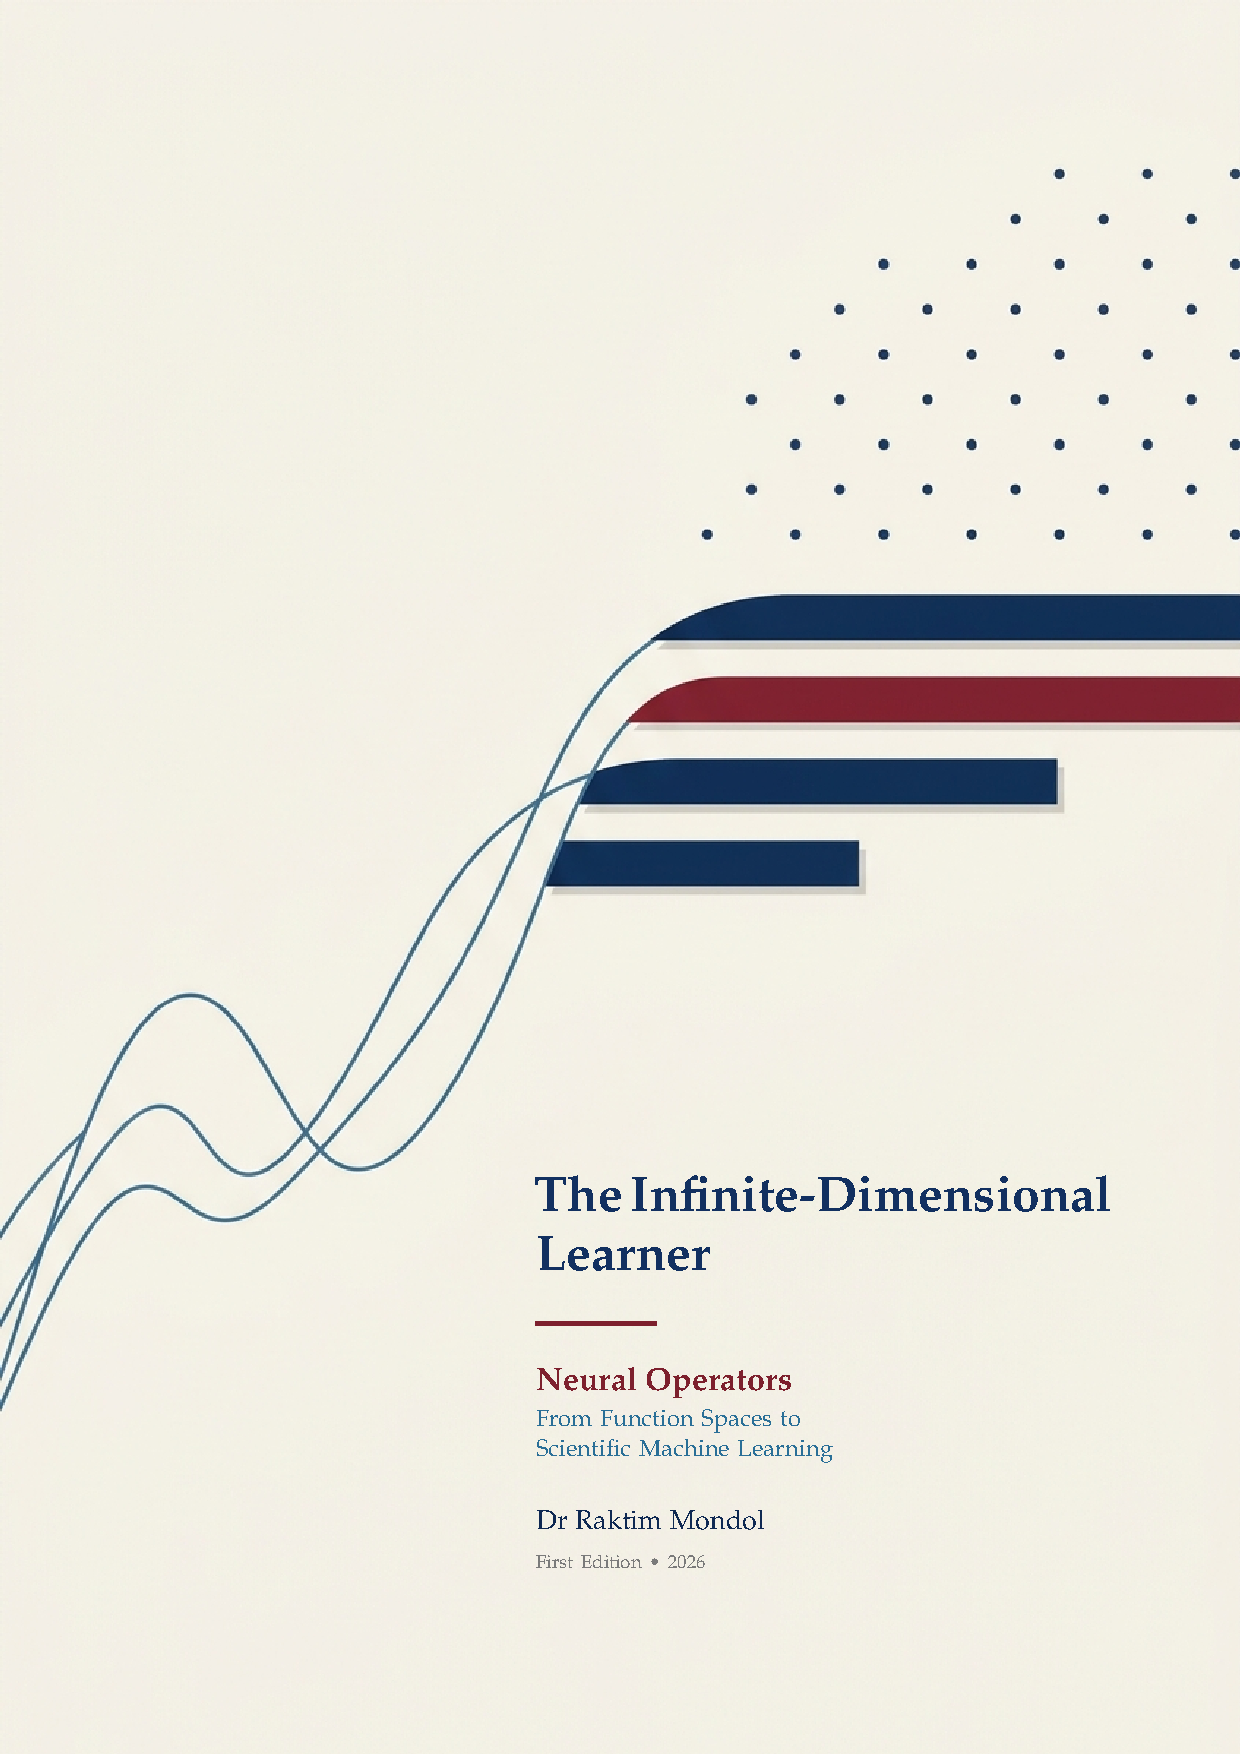
\includepdf[pages=1,pagecommand=\thispagestyle{empty}]{covers/cover.pdf}
\cleardoublepage

% =====================================================================
\frontmatter
% =====================================================================
\begin{titlepage}
\centering
{\color{primary}\hrule height 2pt}\par\vspace{2.2em}
{\Huge\bfseries\color{primary} The Infinite-Dimensional Learner}\par\vspace{0.9em}
{\Large\bfseries\color{secondary} Neural Operators: From Function Spaces\\[0.25em]
to Scientific Machine Learning}\par
\vfill
{\large Written by AI,\\[0.25em]
 prompted, edited and reviewed by Dr Raktim Mondol}\par\vspace{0.6em}
{\small First Edition \textbullet{} 2026}\par\vspace{1.4em}
{\color{primary}\hrule height 2pt}
\end{titlepage}

% The verso of the title page carries no marks, so the running head would be an
% empty rule across the top of the page. Plain keeps the folio and drops it.
\thispagestyle{plain}
\vspace*{0.62\textheight}
\begin{flushright}
\begin{minipage}{0.94\textwidth}
\raggedleft\itshape\hyphenpenalty=10000 % 415 pt wide: the quote sets on one line
``The first principle is that you must not fool yourself---and you are the
easiest person to fool.''\\[0.55em]
\upshape\normalsize --- Richard P. Feynman, \textit{Cargo Cult Science}, Caltech, 1974
\end{minipage}
\end{flushright}
\cleardoublepage

\tableofcontents
\cleardoublepage
\listoffigures
\cleardoublepage
\listoftables
\cleardoublepage
\addcontentsline{toc}{chapter}{List of Listings}
\lstlistoflistings
\cleardoublepage

% PREFACE -- the multi-query surrogate problem, scope, intended reader, part
% dependencies, two reading maps, notation conventions, deliberate omissions.
% STATUS: authored; adversarially verified against the .toc and every chapter, section,
% appendix, definition, assumption and table number named below. Four false claims fixed:
% prerequisites sit in Ch. 1's opener, not Sec. 1.1; Ch. 16 does develop one calibration;
% Ch. 22's baseline is FBP; and Ch. 10 assumes CUDA/cuDNN, so no toolchain omission.
\chapter*{Preface}
\addcontentsline{toc}{chapter}{Preface}
\markboth{Preface}{Preface}

Numerical simulation answers one question at a time: data go in, the matching solution field
comes out, and nothing carries over to the next run. The workloads that organize this book do
not pose one question. Shape optimization queries the same equations for thousands of
geometries, ensemble forecasting integrates fifty perturbed initial states twice a day, and
posterior sampling needs a forward evaluation at every proposal a Markov chain makes.
Simulation costs $M\,c_{\mathrm{sim}}(N)$, a surrogate $c_{\mathrm{train}} +
M\,c_{\mathrm{eval}}(N)$: $M$ queries, one classical solve at $N$ unknowns, one training run,
one evaluation per query, as Section~1.1 sets out in \eqref{eq:ch01-cost-bookkeeping}. I wrote
this book because the ledger has a catch: the saving is real only if the surrogate can be asked
the question at all, and a network whose weights are sized for $N$ grid points has no defined
action on $N'$. What must be learned is therefore not a solution but the map from data to
solution --- a map on function spaces, stated without reference to a mesh, evaluated on
whichever discretization a query supplies. Amortization is what changes; the resolution
dependence remains.

Part~I (Chapters~1--9) builds the framework that makes such a map learnable: the Sobolev scale
and compact embeddings that make uniform approximation meaningful in infinite dimensions
(Chapter~2); the proof that the Darcy, Burgers and forced Navier--Stokes solution operators are
continuous, stable and smoothing (Chapter~3); the density theorems of Chen \& Chen and their
DeepONet and generic-operator counterparts (Chapter~4); spectral truncation bounds and
convergence rates for the Fourier neural operator, discretization invariance and the continuum
limit, and physics-informed and Sobolev-regularized objectives (Chapters~5--7); a taxonomy
of what each architecture requires of its target and where its theorems are (Chapter~8), and
the open questions (Chapter~9). Part~II (Chapters~10--16)
turns those objects into tensor programs: layouts, coordinate encoding, losses and normalization
(Chapter~10); complete implementations of DeepONet, the FNO, and the graph and geometry-informed
operators (Chapters~11--13); the canonical benchmarks with their specifications (Chapter~14);
the regimes and failure modes a long run meets (Chapter~15); and export, cost accounting and
calibration (Chapter~16). Part~III (Chapters~17--24) leaves the periodic box for triangulated
surfaces, the sphere, faulted reservoirs, patient-specific ventricles and undersampled
sinograms, scored against the solvers they displace --- finite element, finite volume, implicit
finite difference, spectral-transform, and, in Chapter~22, filtered backprojection --- with
boundary enforcement as the question they make unavoidable (Chapter~23) and a synthesis matrix
closing the argument (Chapter~24). The appendices hold what the text borrows rather than proves,
from the functional-analysis reference (Appendix~A) to the glossary (Appendix~F).

The intended reader is a graduate student or researcher in scientific machine learning who wants
to read a convergence proof and a training log without a translation step. The prerequisites are
those Chapter~1 states before its first section, and they are concrete. From analysis: the
measure-based functional analysis Section~1.2 uses without apology --- a Borel probability
measure on the input space, an expectation of a relative error functional, a worst-case bound
over a compact set held distinct from a risk under a measure --- plus Chapter~2's machinery:
Riesz representation, duality pairings, weak derivatives, Sobolev spaces and their embeddings at
the level of \cite{brezis2011functional, evans2010partial}. From numerical analysis: the
discrete Fourier transform as a change of basis --- what a mode index means, what Nyquist
forbids. From practice: enough PyTorch to read a layer definition --- a \texttt{torch.nn.Module}
and a batched tensor contraction \cite{paszke2019pytorch}, which is also what Chapter~10 assumes.
Readers who command the analysis may treat Chapter~2 as review, as Chapter~1's close suggests;
the rest should not skip it: Part~I states every theorem in that language.

The parts are not independent. Part~II takes Part~I's discretization-invariance framing as its
design criterion: Chapter~10 opens on Definition~6.1 and treats layout, coordinate encoding, loss
and normalization as what a program owes that definition; Chapter~16 asks whether an exported
graph still computes its sizes from the tensor handed to it. The dependence runs the
other way at the end of Part~I, where Chapter~9 turns its unsolved problems into a
specification: the truncation tail becomes a choice of \texttt{modes}, the unrolled loss a
training recipe, the Lipschitz product a divergence the practitioner must notice by hand.
Part~III uses both. Chapter~17 names the concessions of Chapters~1--16 --- torus, unit square,
one application of the operator --- and withdraws them at mesh sizes two to five orders above
those Chapter~16 counted. Each application chapter needs Part~II for the artifact and Part~I for
the hypothesis it cannot escape: the bounds of Chapters~4--6 are stated under a compactness
hypothesis on the support of the training measure (Assumption~9.1), so out-of-distribution
behavior is recorded in Part~III as observed, not bounded.

Two routes are worth prefiguring. For a one-semester course, Chapters~1--6 form the spine; add
Chapters~10 and~12 for the implementation, Appendix~B as the laboratory exercise --- its $0.0141$
relative $L^{2}$ errors on the $64$- and $256$-point grids, caveat attached --- and Chapter~14
with Appendix~C for the specifications a run needs. One application chapter, read against
Chapter~17's ledger, closes the course; Chapter~19 or~20 suits best. Where time is short,
Chapter~8's theorem ledger is the hour best spent and Chapter~9 the discussion. For a
practitioner with a model to train, begin at Chapter~10; take Chapter~12 (Section~12.4 for the
official library), Chapter~11 if a branch-and-trunk fit is intended, Chapter~13 for meshes, then
Chapter~15 with Appendix~D before the first long run and Chapter~16 before serving. Read two
theory chapters regardless: Chapter~6 for what a discretization owes the continuum, Chapter~5
for what the choice of modes costs. Chapter~4's three-term split explains a validation curve
that flattens while the training loss still falls; Chapter~9, why a rollout that looks stable is
not bounded.

Notation is fixed once, in \emph{Notation and Conventions} and its Table~\ref{tab:notation-master},
which gives the symbols in three blocks: Part~I's infinite-dimensional objects, Part~II's tensor
layouts, Part~III's physical quantities. Its rule is that a letter reused across parts carries
its ambiguity in its own row rather than silently: $\mu$ is the input measure, Chapter~10's
pointwise ensemble mean, and, with a phase subscript, a Part~III viscosity; $M$ counts queries in
Chapter~1, ensemble members in Part~II, detector views in Chapter~22. Where a chapter's gloss and
the table differ, the table governs. Appendix~E inverts it: Section~E.1 indexes the variants (GNO,
GINO, AFNO, U-FNO, PINO) by the chapter that builds each, Section~E.2 maps the
principal symbols to the equation or section at which they begin to do work.

What the book does not cover deserves the same directness. There is no learning theory beyond
Chapter~9's entropy arithmetic: Chapter~4's density theorems are existence results whose limits
Section~4.4 inventories, and optimization error, Section~1.3's fourth term, is
handled empirically in Chapter~15 and Appendix~D alone. Supervision is by paired fields; the one
route around it is PINO's weak-form residual objective (Chapter~7, Section~14.4), whose reported
gains are benchmark outcomes, not theorems. Sparse or partially observed labels are not treated:
DeepONet's sensors (Section~11.2) restrict where an input is read, not whether an output is
known, and Chapter~22's sparse-view and limited-angle protocols thin the sinogram, not the
labels. Inverse problems appear as workloads and as pointers (Sections~1.2, 3.1, 17.2 and~20.4;
Chapter~9's fallback to Bayesian formulations), since this book learns forward maps, not
posteriors; the one inverse problem it solves, Radon inversion in Chapter~22, is linear.
Uncertainty quantification is likewise a use case (Chapter~20's Monte Carlo sweeps) and a
roadblock (Chapter~24's bound on distribution shift), not a methodology: no posterior is
estimated, no coverage guarantee proved, and the only calibration developed is
Chapter~16's, of surrogate error against its labeling budget. Classical solvers
are baselines and label producers; Section~23.1's account of why a conforming
discretization carries its boundary conditions by construction is the one place their mechanics
matter; elsewhere they are priced rather than derived: Chapter~17 charges meshing as an
unreported cost, the turbulence and capillary-pressure closures only as far as the surrogate's
data depend on them. Software engineering stops where Chapter~16 stops: no cluster scheduling,
data pipeline or model-versioning practice, and no tuning of a vendor's kernels beyond the CUDA
and cuDNN vocabulary Chapter~10 assumes. Finally, every surrogate here is deterministic: no
generative model --- diffusion, flow, or sampler-based --- is treated, and \emph{diffusion} in
Part~III names a physical coefficient.

Three conventions govern the text, which is why those omissions are named: numbers travel with
the configuration that produced them, theorems with their hypotheses, and a claim whose
provenance cannot be recovered is recorded as unestablished rather than smoothed. Where the
record is silent --- a baseline timing behind a published speedup --- the book says so.

% NOTATION -- master table, complete. The functional-analysis and spectral-
% truncation symbols of Part I, among them the retained mode set Z_{k_max} and
% the smoothing order alpha of Ch. 5, whose Appendix B diffusivity namesake is
% disambiguated in the same row; the tensor-layout symbols of Part II, used by
% Chapters 10--16; and the physical symbols of Part III, used by
% Chapters 17--24. Every symbol whose name is reused across parts carries its
% ambiguity in its own row, as the chapters themselves print it.
\chapter*{Notation and Conventions}
\addcontentsline{toc}{chapter}{Notation and Conventions}
\markboth{Notation and Conventions}{Notation and Conventions}

Symbols are used consistently throughout the book. The conventions below are
established in Part~I and reused without restatement in Parts~II and~III, where
the second block of the table records the array conventions every implementation
is written in and the third the physical quantities the application chapters
solve for. Where the same letter carries two meanings in different parts, the row
for the later meaning names the earlier one where space allows --- the reuses the
reader is most likely to meet are $p$ (integrability exponent, DeepONet latent
width, parameter count), $\sigma$ (activation, pointwise spread, Sobolev order in
$H^\sigma$), $m$
(sensor count, modes per band edge), $P$ (the DeepONet query-point count, and the projectors $P_N$,
$P_{k_{\max}}$), and $L$ (layer count, body length) --- but the flagging is a
promise about visibility, not a proof that no symbol anywhere does double duty.

% {\raggedright\arraybackslash} on the definition column: the cells are narrow
% single paragraphs and justification leaves rivers and underfull lines in them
% (pattern used for every other table column in the book).
{\small
\begin{xltabular}{\textwidth}{@{}l>{\raggedright\arraybackslash}X@{}}
\caption{\textbf{Notational conventions: the infinite-dimensional objects, the tensors that realize them, and the physical symbols the applications are written in.}}
\label{tab:notation-master}\\
\toprule
\textbf{Symbol} & \textbf{Mathematical Definition and Context} \\
\midrule
\endfirsthead
\multicolumn{2}{r}{\textit{Table~\ref{tab:notation-master}, continued}}\\
\toprule
\textbf{Symbol} & \textbf{Mathematical Definition and Context} \\
\midrule
\endhead
\midrule
\multicolumn{2}{r}{\textit{Table~\ref{tab:notation-master}, continued on the next page}}\\
\endfoot
\bottomrule
\endlastfoot
$\Omega \subset \mathbb{R}^d$ & Open, bounded domain with Lipschitz boundary $\partial\Omega$, or flat torus $\mathbb{T}^d$. \\
$L^p(\Omega; \mathbb{R}^{d_v})$ & Lebesgue space of measurable functions with norm $\|u\|_{L^p} = (\int_\Omega |u(x)|^p dx)^{1/p}$. \\
$H^s(\Omega) = W^{s,2}(\Omega)$ & Sobolev space of functions whose weak derivatives up to order $s$ reside in $L^2(\Omega)$. \\
$C^k(\overline{\Omega})$ & Space of $k$-times continuously differentiable functions equipped with uniform norm. \\
$X, Y, \mathcal{A}, \mathcal{U}$ & Real or complex Banach or Hilbert spaces. \\
$\mathcal{L}(X, Y)$ & Space of bounded linear operators from $X$ to $Y$ with operator norm $\|T\|_{\mathcal{L}(X,Y)}$. \\
$\langle \cdot, \cdot \rangle_{X^*, X}$ & Duality pairing between Banach space $X$ and its continuous topological dual $X^*$. \\
$\mathcal{F}, \mathcal{F}^{-1}$ & Continuous or discrete Fourier transform and its inverse. The convention is fixed once: $\hat{u}(k) = \int u(x)\, e^{-2\pi i k \cdot x}\,dx$, so $\{e^{2\pi i k \cdot x}\}$ is the $L^2$-orthonormal basis on the torus, and the DFT is unnormalized forward with $1/N$ on the inverse --- PyTorch's default \texttt{norm="backward"} --- unless a passage says otherwise. The aliasing identity of Part~I, the Parseval statements in Appendix~A, and the coefficient magnitudes archived in Appendix~B all turn on this choice. \\
$\mathbb{T}^d \cong [0, 1)^d$ & $d$-dimensional periodic torus identifying opposite boundaries. \\
$D^\alpha u$ & Weak partial derivative for multi-index $\alpha \in \mathbb{N}_0^d$. \\
$\mathcal{M}_N = \{x_j\}_{j=1}^{N}$, $P_N$ & A discretization of $\Omega$ and the restriction operator sending $a$ to its nodal values; \eqref{eq:ch21-grid-layout} and \eqref{eq:ch21-node-layout} are its two array forms. \\
$Z_{k_{\max}}$, $k_{\max}$ & The retained mode set of Part~I, $Z_{k_{\max}} = \{k = (k_1, \dots, k_d) \in \mathbb{Z}^d : |k_j| \le k_{\max, j},\ j = 1, \dots, d\}$ of \eqref{eq:ch05-modeset} --- a box rather than the ball $\{|k| \le k_{\max}\}$, because a product of contiguous index ranges is what a batched transform can slice without gathering scattered entries. It contains $|Z_{k_{\max}}| = \prod_{j=1}^d (2k_{\max, j}+1)$ modes, one complex $d_v \times d_v$ multiplier each, and $k_{\max}$ without a subscript denotes the common cutoff, the case assumed in Theorem~\ref{thm:fno_convergence}. The partial sum $P_{k_{\max}}$ of \eqref{eq:ch05-projection} projects onto the span of $Z_{k_{\max}}$, so it is a spectral projection and not the nodal restriction $P_N$ above, and \eqref{eq:ch05-projection-bound} sums its tail over $k \notin Z_{k_{\max}}$, exactly the modes the box projection discards --- an earlier drafting summed over the ball, whose relation to the box complement runs only one way. Part~II's $Z_m$ of \eqref{eq:ch23-corners} is this same object realized on the half-spectrum, where the two corners carry the cutoffs $m_x, m_y$ in place of the symmetric ranges $|k_j| \le k_{\max, j}$. \\
$\alpha$ & The smoothing order, or regularity gain, of an operator: Theorem~\ref{thm:fno_convergence} assumes $\mathcal{G} : H^s(\mathbb{T}^d; \mathbb{R}^{d_a}) \to H^{s+\alpha}(\mathbb{T}^d; \mathbb{R}^{d_u})$ with $\alpha > 0$ on a compact set $K$; that gain, composed with the compactness, bounds the output regularity $s+\alpha$ that sets the exponent of the truncation term $C_1 k_{\max}^{-(s+\alpha)}$ in \eqref{eq:ch05-error-decomposition} --- the exponent is the regularity of the target \emph{field}, not the gain alone, per \eqref{eq:ch05-projection-bound}. It is a hypothesis about the operator being learned, not a property of the architecture. Not the diffusivity $\alpha = 0.01$ of the periodic heat equation \eqref{eq:appb-pde} in Appendix~\ref{app:b}: there $\alpha$ is a coefficient of the equation, and the mode damping $e^{-\alpha (2\pi k)^2 T}$ of its solution operator \eqref{eq:appb-multiplier} decays faster than any power of $k$, so that number is not the smoothing order of the operator it defines. Nor the multi-index $\alpha \in \mathbb{N}_0^d$ of $D^\alpha u$ above. Three further readings are in use locally: the H\"older exponent of $C^{j,\alpha}$ in the supercritical Sobolev embedding, the miss level $\alpha$ of a conformal interval of coverage $1-\alpha$ in Part~III, and the rollout-horizon multiple $\alpha K$ of Part~II's pushforward training. \\
\midrule
\multicolumn{2}{l}{\textit{Tensor-layout conventions of Part~II}}\\
\addlinespace
$B$ & Batch size; the leading axis of every tensor, and the only one carrying no operator semantics. \\
$C$ & Channel axis of a grid tensor --- the $d_a$ input or $d_u$ output components of Part~I, per node. \\
$C_{\text{in}}, C_{\text{out}}$ & Channel counts at the two ends of one layer; \eqref{eq:ch21-augment} raises $C_{\text{in}}$ to $C_{\text{in}} + d$. \\
$H, W$ & Height and width of a two-dimensional grid; in $d$ dimensions they are the $N_1, \dots, N_d$ of \eqref{eq:ch21-grid-layout}. \\
$d_v$, $L$ & The lifted channel width --- Part~I's $d_v$ carried through the network as \texttt{hidden\_channels} --- and the number of operator layers. \\
$N$, $N_{\text{nodes}}$ & Node count $\prod_j N_j$ of a discretization, and the per-sample node count of a mesh layout. \\
$X \in \mathbb{R}^{B \times C \times N_1 \times \cdots \times N_d}$ & Structured-grid (channel-first) layout; $\prod_j N_j = N$, $C = d_a$ at the input and $C = d_u$ at the output. \\
$X_{\text{nodes}} \in \mathbb{R}^{B \times N_{\text{nodes}} \times C}$ & Point-cloud (mesh) layout, with $X_{\text{coords}} \in \mathbb{R}^{B \times N_{\text{nodes}} \times d}$ carrying the positions $x_j$. \\
$w_j$, $\Delta x$ & Quadrature weights --- cell volumes or Voronoi dual areas --- and the spacing of an equispaced grid, $w_j = \Delta x^d$. \\
$m_x, m_y$ & Retained Fourier modes along $H$ and $W$; written $k_x, k_y$ in Figure~\ref{fig:fno_spectral} and \texttt{modes1}, \texttt{modes2} in the code. \\
$Z_m$, $R^{(1)}, R^{(2)}$ & The retained mode set of \eqref{eq:ch23-corners} and the two complex weight tensors of \eqref{eq:ch23-Rtensors}, indexed by mode, not by grid point. \\
$m$, $P$, $p$, $h$ & DeepONet's sensor count, query-point count, latent width (\texttt{latent\_p}), and hidden width (\texttt{hidden\_dim}). \\
$r$, $\mathcal{N}_r(i)$, $N_{\text{edges}}$ & GNO neighborhood radius, the ball $\mathcal{B}_r(x_i)$ as a node set, and the edge count of \texttt{edge\_index}. \\
$M$, $\mu(x)$, $\sigma(x)$ & Training-ensemble size and the pointwise mean and standard deviation of \eqref{eq:ch21-normalize}; the $\mu$ elsewhere in the book is the input \emph{measure} they estimate. \\
\midrule
\multicolumn{2}{l}{\textit{Physical symbols of Part~III}}\\
\addlinespace
$Q$, $Q^{\star}$ & Query count of a multi-query workload and its break-even value, \eqref{eq:ch31-ledger} and \eqref{eq:ch38-crossover}; Part~I writes the same quantity $M$ in \eqref{eq:ch01-cost-bookkeeping}. \\
$\mathbf{u}$, $\rho$, $\mu$, $\mu_t$ & Velocity and density of the classical solvers Part~III compares against, their molecular viscosity $\mu$ and eddy viscosity $\mu_t$; a subscript $\alpha$ on $\mu_\alpha$ or $\rho_\alpha$ labels a \emph{phase}, not the measure $\mu$ or the mean $\mu(x)$ above. \\
$\mathbf{K}(x)$, $\phi(x)$ & Heterogeneous permeability tensor and porosity of the two-phase Darcy system \eqref{eq:ch34-cons-w}; $\phi$ there is porosity, while $\phi$ in \eqref{eq:ch33-momentum} is latitude. \\
$S_w$, $S_g$, $S_{\mathrm{CO}_2}$ & Phase saturations with $S_w + S_g = 1$; $S_{\mathrm{CO}_2}$ is the reservoir-engineering name for the gas saturation $S_g$, used in Figure~\ref{fig:vol3_sub}. \\
$k_{r\alpha}$, $\lambda_\alpha$, $f_g$, $p_c$ & Relative permeability in $[0,1]$ from the van Genuchten or Brooks--Corey closure, the phase mobility $\lambda_\alpha = k_{r\alpha}/\mu_\alpha$, the fractional flow $f_g$ of \eqref{eq:ch34-mobility}, and the capillary pressure $p_g - p_w$. \\
$\mathbf{u}_\alpha$, $q_\alpha$, $s$ & Darcy phase flux \eqref{eq:ch34-flux}, the well source or sink, and the front speed of the jump condition \eqref{eq:ch34-rh}, across which $[\,\cdot\,]$ denotes the jump. \\
$V_m$, $C_m$, $\chi$, $I_{\text{ion}}$, $I_{\text{stim}}$ & Transmembrane voltage, membrane capacitance per unit area, surface-to-volume ratio, and the ionic and stimulus current densities of the monodomain equation \eqref{eq:monodomain}. \\
$\mathbf{w}$, $k$, $a$, $b$, $\epsilon_0$, $\mu_1$, $\mu_2$ & Recovery variable of \eqref{eq:ch35-recovery} --- distinct from the quadrature weights $w_j$ above --- and the dimensionless Aliev--Panfilov kinetic constants of \eqref{eq:ch35-ion}; the $k$ there is a kinetic parameter, not the mode index of \eqref{eq:ch05-modeset} or the turbulent energy below. \\
$\mathbf{D}(x)$, $\sigma_l$, $\sigma_t$, $\mathbf{f}_0$ & Cardiac diffusion tensor \eqref{eq:ch35-dtensor} built from longitudinal and transverse conductivities along the fiber direction $\mathbf{f}_0$; $\mathcal{D} = \mathbf{D}/(\chi C_m)$ and $D_{\max} = \max_x \rho_{\max}(\mathcal{D}(x))$ set the step \eqref{eq:ch35-cfl}. \\
$h$, $\Delta t$, $T$, $W(h,T)$ & Mesh width, time step, simulated horizon, and the discretization work \eqref{eq:ch35-cost}; $h$ here is a length in micrometers, not the DeepONet hidden width of the block above. \\
$Re$, $U_\infty$, $L$, $\delta$, $y^{+}$, $u_\tau$, $\tau_w$ & Reynolds number \eqref{eq:ch32-reynolds}, freestream speed, body length, boundary-layer thickness, wall-normal distance in viscous units and friction velocity \eqref{eq:ch32-yplus}, and wall shear stress \eqref{eq:ch32-wss}. \\
$C_d$, $C_l$, $F_d$, $F_l$, $A_{\text{ref}}$ & Drag and lift coefficients with their forces and reference area, defined by the surface integral \eqref{eq:ch32-force-coeff}; $k$ and $\omega$ in the closure \eqref{eq:ch32-reynolds-stress} are turbulent kinetic energy and specific dissipation. \\
$\mathbf{u}_h$, $w$, $\theta$, $f$, $\Omega_{\text{rot}}$ & Horizontal and vertical wind, potential temperature, Coriolis parameter $f = 2\Omega_{\text{rot}}\sin\phi$, and planetary rotation rate of \eqref{eq:ch33-momentum}--\eqref{eq:ch33-pottemp}; $\theta$ there is a field, not the network parameter of Part~II. \\
$\mathcal{R}$, $\mathbf{M}$, $\mathcal{A}$, $p(\theta,s)$ & Radon transform, restriction to the $M$ measured view angles, sampled forward operator $\mathcal{A} = \mathbf{M}\mathcal{R}$, and sinogram of \eqref{eq:ch36-radon}, with detector position $s$, detector frequency $\omega$, and moments $m_k$ \eqref{eq:ch36-moment}; this $M$ counts views, not ensemble members. \\
$\mathrm{ACC}$, $\mathrm{RQE}$, $\mathcal{T}$ & Anomaly correlation \eqref{eq:ch33-acc} and relative quantile error \eqref{eq:ch33-rqe}; $\mathcal{T}(w) = \int_\Omega w\,\mathrm{d}x$ the conserved total whose defect $\Delta_{\mathcal{T}}$ \eqref{eq:ch38-defect} measures. Image quality is reported as PSNR, SSIM, and RMSE in Hounsfield units (HU), \eqref{eq:ch36-metrics}. \\
\end{xltabular}
}

% NOTE: the copy of the notation table that once opened Ch. 1 was removed; this
% front-matter table is the single reference for the whole book.
% The Part II tensor-layout block and the Part III physical block extend it with
% the symbols as actually printed in the chapters they name. The two closing
% rows of the Part I block, for the retained mode set and the smoothing order,
% follow eq. (5.5) and Theorem 5.2 of Ch. 5 and the use of those symbols in
% Ch. 2, Ch. 6, Appendix A and Appendix B.


% =====================================================================
\mainmatter
% =====================================================================

% ------------------------------------------------------------------ PART I
\part{Mathematical Foundations: Functional Analysis, Operator
Approximation, and Spectral Theory}
\label{part:1}
% Part I opener: the scope of Chapters 1--9, the mathematical foundations.
\noindent Part~I develops the mathematical foundations of operator learning in
infinite-dimensional function spaces. Classical finite-dimensional statistical
learning theory does not reach a map between function spaces, so the first task
is to build the functional-analytic framework in which a neural operator can be
understood as a map between Banach and Hilbert spaces: completeness, duality,
compact embeddings, and the Sobolev regularity that determines what any
approximation can hope to control. On that ground Part~I examines the
well-posedness of parametric partial differential equations (PDEs), the
representation of linear and nonlinear solution operators through Green's
kernels, and the classical universal approximation theorems for nonlinear
operators of Chen and Chen (1995). Contemporary architectures are then analyzed
together rather than separately, with a unified treatment of the Generic Neural
Operator framework (Kovachki et al., 2023), DeepONet (Lu et al., 2021), and the
Fourier Neural Operator (Li et al., 2021). The emphasis falls on discretization
invariance, spectral truncation error bounds, Sobolev-norm convergence rates,
and the mathematical consistency of physics-informed operator surrogates. What
is proved here supplies the vocabulary that Part~II implements and the claims
Part~III tests against physical data.

% Chapter 1: Introduction: The Paradigm Shift to Infinite-Dimensional Learning
% Part I of the book.

\chapter{Introduction: The Paradigm Shift to Infinite-Dimensional Learning}
\label{ch:part1-introduction-the-paradigm-shift-to-infinit}
\label{sec:intro}
% -----------------------------------------------------------------------------

Numerical simulation answers one question at a time: given a permeability field, an
initial state, or boundary data, a
\index{finite volume method (FVM)}\emph{finite volume method} (FVM) or a
\index{finite element method (FEM)}\emph{finite element method} (FEM) returns the matching
solution field, and changing one coefficient carries nothing over from the previous solve.
The workloads that motivate this book do not pose single questions. Shape optimization
queries the same governing equations for thousands of candidate geometries, ensemble weather
forecasting integrates a perturbed initial condition many times, and reservoir risk
assessment samples a distribution over subsurface heterogeneity; every setting in Part~III
asks for many solutions of one operator. We call this the
\index{multi-query surrogate problem}\index{operator learning}\emph{multi-query surrogate problem}: the quantity of interest is not a solution but the map from data to solution, and
it must be evaluated at whatever resolution each query requires.

Stretching a conventional network over such a workload does not remove the mismatch, because
these architectures are maps between fixed-dimensional Euclidean spaces: parameter count,
weight-tensor shapes, and the physical meaning of each activation are all set by the number
of grid points present at training time. The alternative developed in this book takes the
\emph{operator} as the object of learning---a map defined on function spaces, written down
without reference to a mesh, then evaluated on whichever discretization a query supplies.
Parts~II and~III inherit that change of target, and it is not a change of vocabulary: it
raises three questions finite-dimensional learning theory never asks. What spaces does the
network consume and produce, and how much regularity do their elements carry? What must the
target map satisfy for approximation to be possible at all? And what does it mean for a
machine to apply a map not defined on a finite list of numbers?

This chapter states the problem and the shape of its answers; it proves almost
nothing. The arguments come from the rest of Part~I.
\chapref{ch:part1-function-spaces-duality-and-sobolev-regula} fixes the spaces, the norms,
and the compactness machinery;
\chapref{ch:part1-partial-differential-equations-as-solution} verifies that the solution maps
of Darcy flow, Burgers' equation, and Navier--Stokes carry the continuity and smoothing
properties the theory demands;
\chapref{ch:part1-operator-approximation-theory-and-universa} supplies the density results;
and \chapref{ch:part1-the-fourier-neural-operator-spectral-theor} with
\chapref{ch:part1-discretization-invariance-and-continuum-li} deliver an architecture and a
mesh-independence statement. The reader should bring measure-based probability, a first
course in functional analysis, Sobolev spaces at the level of
\cite{brezis2011functional, evans2010partial}, the discrete Fourier transform, and enough
PyTorch to read a layer definition; results Part~I invokes without proof are collected in
Appendix~\ref{app:a}.

\section{The Multi-Query Bottleneck in Simulation-Based Science}

Classical deep learning architectures---multilayer perceptrons
\index{multilayer perceptron (MLP)}(MLPs), convolutional neural networks
\index{convolutional neural network (CNN)}(CNNs), recurrent neural networks
\index{recurrent neural network (RNN)}(RNNs)---are formulated as maps between
finite-dimensional Euclidean spaces,
\begin{equation}
  \label{eq:ch01-euclidean-map}
  f_\theta : \mathbb{R}^{d_{\text{in}}} \longrightarrow \mathbb{R}^{d_{\text{out}}}, \qquad \theta \in \Theta \subset \mathbb{R}^p,
\end{equation}
with $p$ trainable parameters and with the input and output dimensions $d_{\text{in}},
d_{\text{out}}$ fixed by the architecture before any data are seen. Equation
\eqref{eq:ch01-euclidean-map} is not one design's limitation but the shared contract of the
class: a tensor of size $d_{\text{in}}$ must arrive with its entries in a prescribed order.

Applied to systems governed by \index{partial differential equation (PDE)}\emph{partial
differential equations} (PDEs), such a model therefore consumes discrete approximations of
continuous fields, sampled at fixed spatial or temporal locations $\{x_i\}_{i=1}^{N}
\subset \Omega$: an input field $a$ enters as the vector $\big(a(x_1), \dots, a(x_N)\big)
\in \mathbb{R}^{N d_a}$, so that $d_{\text{in}} = N d_a$, with $d_a$ the number of components
of $a$ and $d_u$ the number of components of the output. The consequence is that the
learned parameters $\theta$ remain intrinsically coupled to the \index{mesh resolution!coupling of network parameters to}mesh resolution $N$, the grid
topology, and the sampling geometry used during training. Refine the resolution
($N \to N'$), deform the mesh, or move the sensors, and the finite-dimensional model becomes
inapplicable without ad hoc interpolation, retraining, or loss of fidelity. The usual repair,
re-interpolation, is the least defensible: resampling a surrogate's output onto $N'$ points
introduces an error training never saw or bounded, so the reported accuracy describes grid
$N$, not the field.

The economics define what the machinery of this book is for. Let $M$ be the number of queries, let $c_{\mathrm{sim}}(N)$ be the cost of one classical
solve at $N$ unknowns, let $c_{\mathrm{train}}$ be the one-time cost of building a surrogate,
and let $c_{\mathrm{eval}}(N)$ be the cost of one surrogate evaluation:
\begin{equation}
  \label{eq:ch01-cost-bookkeeping}
  C_{\mathrm{sim}}(M, N) = M\, c_{\mathrm{sim}}(N),
  \qquad
  C_{\mathrm{sur}}(M, N) = c_{\mathrm{train}} + M\, c_{\mathrm{eval}}(N).
\end{equation}
Equation \eqref{eq:ch01-cost-bookkeeping} is arithmetic, not a theorem, and it invites three
qualifications. First, the surrogate wins only when $c_{\mathrm{eval}}(N) <
c_{\mathrm{sim}}(N)$, with crossover at $M^{\star} = c_{\mathrm{train}} /
\big(c_{\mathrm{sim}}(N) - c_{\mathrm{eval}}(N)\big)$; a single design check should still be
handed to a classical solver \cite{leveque2002finite, quarteroni2008numerical}. Second,
$c_{\mathrm{train}}$ is not free of the solver it replaces, because supervised training
produces its paired samples by running that solver repeatedly; amortization presupposes data
generation as a sunk cost shared across many downstream queries.
Third, and most important for what follows, $c_{\mathrm{eval}}(N)$ still grows with $N$. A
spectral forward pass costs $\mathcal{O}(N \log N)$ operations on a uniform periodic grid,
whereas a branch-and-trunk network costs an amount set by its widths and by the number of
sensor and query points rather than by the evaluation grid
\cite{li2021fourier, lu2021learning}. The gain of operator learning is amortization of a
family of solves, not removal of the resolution dependence.

What the fixed-mesh formulation actually forfeits is not speed but scope. Three distinct
failures are entangled in \eqref{eq:ch01-euclidean-map} once the mesh changes: resolution
coupling, since weights sized for $N$ nodes have no defined action on $N'$ nodes; geometry
coupling, since convolutional weights are indexed by lattice offsets, so a refinement shrinks
their physical footprint---the argument made quantitatively in
\chapref{ch:part1-discretization-invariance-and-continuum-li}; and a semantic failure often missed in
benchmarks, namely that a network trained on one sampling of one field learns \emph{a}
solution rather than the rule that generates solutions from data.
The first two can be patched by re-interpolation at some cost in accuracy; the third cannot,
because the network represents an object the application does not need. Diagnosing
it requires a target defined independently of any discretization, which is the next
section's subject.

\section{Solution Operators as Targets of Learning}

Scientific and physical laws operate on continuous fields. Velocity fields satisfy
$\mathbf{u}(\cdot, t) \in (L^{2}(\Omega))^{d}$, temperature distributions satisfy
$T(\cdot) \in H^{1}(\Omega)$, and permeability tensors satisfy
$\mathbf{K}(\cdot) \in L^{\infty}(\Omega; \mathbb{R}_{\text{sym}}^{d \times d})$, where
$\Omega \subseteq \mathbb{R}^{d}$ is the spatial domain, $L^{p}(\Omega)$ denotes functions
whose $p$-th power is integrable, and $H^{s}(\Omega)$ denotes the \index{Sobolev space}Sobolev space of elements
with $s$ derivatives in $L^{2}(\Omega)$; \chapref{ch:part1-function-spaces-duality-and-sobolev-regula}
develops both. Each of these is an element of an infinite-dimensional vector space, and the
map that carries an initial state, a boundary forcing, or a coefficient field to the system
state at time $t$ is a \textbf{solution operator}
\index{solution operator}
\begin{equation}
  \label{eq:ch01-solution-operator}
  \mathcal{G} : \mathcal{A} \longrightarrow \mathcal{U},
\end{equation}
where the \index{A@$\mathcal{A}$ (input function space)}input space $\mathcal{A}$ and the
\index{U@$\mathcal{U}$ (output function space)}output space $\mathcal{U}$ are infinite-dimensional Banach or Hilbert function
spaces over $\Omega$
\cite{kovachki2023neural, stuart2010inverse}. Equation \eqref{eq:ch01-solution-operator} is
deliberately terse, and the two spaces are usually different: for the Darcy problem treated
in \chapref{ch:part1-partial-differential-equations-as-solution}, the coefficient enters from
$L^{\infty}(\Omega)$ while the solution lands in $H^{1}_{0}(\Omega)$. The same notation covers
the time-$t$ map $u_{0} \mapsto u(\cdot, t)$, the one-step map
$u(t) \mapsto u(t + \Delta t)$ used for autoregressive rollouts, and parameter-to-state maps,
in which finitely many physical parameters enter as functions on $\Omega$---which is why the
target is stated as \eqref{eq:ch01-solution-operator} rather than as a
particular PDE.

Contrast this with the \index{Physics-Informed Neural Network (PINN)}physics-informed neural
network (PINN), in which a network approximates
\emph{one} solution by minimizing a residual at collocation points
\cite{raissi2019physics}. A PINN's unknown is a field; the operator learner's unknown is a
map, so a new input case is a forward pass rather than a new optimization. Because the
application's queries are drawn from a distribution, training minimizes
an expected loss under an \index{input measure}input measure
$\mu \in \mathcal{P}(\mathcal{A})$, where $\mathcal{P}(\mathcal{A})$ is the set of Borel
probability measures on $\mathcal{A}$,
\begin{equation}
  \label{eq:ch01-risk}
  \mathcal{R}(\theta)
  = \mathbb{E}_{a \sim \mu}
    \left[ \frac{\big\|\mathcal{G}_{\theta}(a) - \mathcal{G}(a)\big\|_{\mathcal{U}}^{2}}
                {\big\|\mathcal{G}(a)\big\|_{\mathcal{U}}^{2}} \right],
    \qquad a \in \mathcal{A},
\end{equation}
and the normalization in \eqref{eq:ch01-risk} makes errors comparable across resolutions and
across magnitudes---the relative-$L^{2}$ metric used throughout Parts~II and~III. Approximation
theory, however, states its guarantees in a different language, as a worst-case bound $\sup_{a \in K} \|\mathcal{G}_{\theta}(a) -
\mathcal{G}(a)\|_{\mathcal{U}} < \varepsilon$ over a compact set $K \subset \mathcal{A}$. The
two are related but not interchangeable: the supremum controls the risk only when $\mu$ gives
$K$ full measure and $\|\mathcal{G}(a)\|_{\mathcal{U}}$ stays bounded away from zero, whereas
the risk controls the supremum nowhere. The gap between them is the statistical
error that \chapref{ch:part1-operator-approximation-theory-and-universa} and
\chapref{ch:part1-open-theoretical-problems-and-mathematical} return to, and a surrogate that
satisfies one and not the other is a familiar engineering failure.

Turning \eqref{eq:ch01-solution-operator} into something trainable means proposing a
parametric family $\mathcal{G}_{\theta}$, $\theta \in \Theta \subset \mathbb{R}^{p}$, with
three requirements: the parameter space $\Theta$ is defined independently of any
discretization; each $\theta$ determines an operator on the continuum spaces
$\mathcal{A}$ and $\mathcal{U}$; and the resulting map is continuous in the norm of
$\mathcal{U}$. Continuity is not a formality. Networks assemble bounded linear maps and
Lipschitz activations, so every architecture considered here produces continuous
$\mathcal{G}_{\theta}$, while a discontinuous target cannot be approximated uniformly on any
set containing the jump---which is why the density theorems of
\cite{chen1995universal, kovachki2021universal} all place continuity of $\mathcal{G}$ among
their hypotheses. The requirement pushes the burden of proof upstream: before asking whether
the architecture class is rich enough, we must ask whether the solution map is continuous and
on which subsets of $\mathcal{A}$ it is---the content of
\chapref{ch:part1-partial-differential-equations-as-solution}, resting on the regularity
theory of the chapter before it.

\takeaway{The Fundamental Objective of Operator Learning}{Rather than approximating a specific solution vector on a fixed discretization, neural operator theory seeks to parameterize a family of mappings $\mathcal{G}_\theta: \mathcal{A} \to \mathcal{U}$ such that $\mathcal{G}_\theta$ is continuous, mesh-independent, and capable of being queried on arbitrary discretizations without retraining.}

Several realizations of that program recur throughout the book, each trading one kind of
coupling for another. \index{DeepONet}DeepONet (Deep Operator Network) reads the input at $m$ fixed
sensors through a branch network and synthesizes the output at arbitrary query coordinates
through a trunk network, so the output side is mesh-free while the input side stays
sensor-bound \cite{lu2021learning}. The
\index{neural operator!generic, integral-kernel architecture}generic neural operator replaces
sensor vectors with learnable integral kernels acting on whole functions
\cite{kovachki2023neural}, and the \index{Fourier neural operator (FNO)}\emph{Fourier neural
operator} (FNO) restricts those kernels to translation-invariant convolution on periodic
domains, which is what makes the continuum operator cheap to evaluate on a grid
\cite{li2021fourier}. The \index{Graph Neural Operator (GNO)}graph neural operator (GNO) and the
\index{Geometry-Informed Neural Operator (GINO)}geometry-informed neural operator (GINO) move the same machinery onto
unstructured point clouds and surface meshes; the
\index{Physics-Informed Neural Operator (PINO)}physics-informed neural operator (PINO) trains
against weak-form residuals rather than paired data alone \cite{li2023geometry, li2021physics}.
Figure~\ref{fig:architectures} in
\chapref{ch:part1-operator-approximation-theory-and-universa} makes the comparison concrete:
panel~(a) is a CNN or MLP whose parameters are bound to one discretization, panel~(b) a
branch-and-trunk network that queries continuous output coordinates through fixed input
sensors, panel~(c) a spectral network that keeps operator semantics under mesh change; and
Table~\ref{tab:comparison} of
\chapref{ch:part1-comparative-theoretical-taxonomy-of-archit} records the same differences
property by property. Part~II holds the implementations, in PyTorch \cite{paszke2019pytorch},
and further descendants---the U-FNO (U-Net-enhanced Fourier neural operator), which interleaves
multi-scale residual blocks with spectral convolution for multiphase flow, and the
\index{adaptive Fourier neural operator (AFNO)}adaptive Fourier neural operator (AFNO) for
global weather---are analyzed
in \chapref{ch:part1-comparative-theoretical-taxonomy-of-archit}, indexed in
Appendix~\ref{app:e}, and applied in Part~III
\cite{wen2022ufno, pathak2022fourcastnet}.

\section{What Changes When the Dimension Is Not Fixed}

Once $\mathcal{A}$ and $\mathcal{U}$ are infinite-dimensional, three intuitions that carry a
finite-dimensional learning theory stop working, and the rest of Part~I exists largely to
replace them. The first is compactness. In $\mathbb{R}^{d}$ a closed and bounded set is
compact, so ``approximate uniformly on the data range'' is an ordinary instruction. In
infinite dimensions the closed unit ball is never compact: bounded sequences need not admit
convergent subsequences at all. Uniform approximation statements must therefore be restricted
to compact subsets $K \subset \mathcal{A}$, and compactness in function space has to be
purchased with regularity rather than assumed. The mechanism is the \index{Rellich--Kondrachov compact embedding}Rellich--Kondrachov
compact embedding, which makes bounded sets in $H^{s}(\Omega)$ precompact in
$H^{t}(\Omega)$ for $s > t \ge 0$; it is proved and put to work in
\chapref{ch:part1-function-spaces-duality-and-sobolev-regula} and is the reason the \index{universal approximation!of operators}density
theorems in \chapref{ch:part1-operator-approximation-theory-and-universa} are stated on
compacta. \index{compactness!failure in infinite dimensions}

The second replacement concerns smoothing, which turns out to be the property that makes an
operator learnable at all. Viscous parabolic problems improve their inputs: for viscous
Burgers' equation with $\nu > 0$, initial data $u_{0} \in L^{2}(\mathbb{T})$ evolve to
$u(\cdot, t) \in H^{s}(\mathbb{T})$ for every $s > 0$. Elliptic problems gain regularity by a
fixed amount: for smooth Darcy coefficients, classical estimates turn $L^{2}$ forcing into an
$H^{2}$ solution, as
\chapref{ch:part1-partial-differential-equations-as-solution} makes explicit. Where the
target behaves as
$\mathcal{G} : H^{s} \to H^{s+\alpha}$ with $\alpha > 0$, the image of a bounded set is
precompact and truncating its range to finitely many Fourier modes costs an amount that
decays like $k_{\max}^{-\alpha}$, which is the content of the spectral convergence result in
\chapref{ch:part1-the-fourier-neural-operator-spectral-theor} \cite{kovachki2021universal}.
Where smoothing fails---inviscid hyperbolic limits, shock formation, transport of
discontinuous data---regularity is destroyed rather than created, and neither the compactness
nor the rate argument survives without new hypotheses. That asymmetry, not a shortage of
layers, is where the honest limits of the theory sit;
\chapref{ch:part1-open-theoretical-problems-and-mathematical} lists it as open.

The third replacement is that a single ``error'' becomes a sum of errors that behave
differently under refinement. Let $\theta^{\star}$ denote a parameter minimizing
$\mathcal{R}$ in \eqref{eq:ch01-risk} within the chosen class, let $\widehat{\theta}$ denote
the parameter produced from finitely many paired samples, and let $\mathcal{G}_{\theta, N}$
denote the discretely implemented operator, with integrals replaced by quadrature on $N$
nodes. Adding and subtracting terms gives
\begin{equation}
  \label{eq:ch01-error-split}
  \begin{aligned}
    \big\|\mathcal{G}(a) - \mathcal{G}_{\widehat{\theta}, N}(a)\big\|_{\mathcal{U}}
    \;\leq\;&
    \underbrace{\big\|\mathcal{G}(a) - \mathcal{G}_{\theta^{\star}}(a)\big\|_{\mathcal{U}}}_{\text{approximation}}
    \\
    &+ \underbrace{\big\|\mathcal{G}_{\theta^{\star}}(a) - \mathcal{G}_{\theta^{\star}, N}(a)\big\|_{\mathcal{U}}}_{\text{discretization}}
    + \underbrace{\big\|\mathcal{G}_{\theta^{\star}, N}(a) - \mathcal{G}_{\widehat{\theta}, N}(a)\big\|_{\mathcal{U}}}_{\text{statistical}} .
  \end{aligned}
\end{equation}
The decomposition \eqref{eq:ch01-error-split} follows from the triangle inequality alone, so
its value lies in which terms the architecture makes separately controllable; authors draw
the cut differently. For DeepONet the natural split is sensor count, trunk basis dimension,
and network error \cite{lanthaler2022error}; for spectral operators, mode truncation appears
as its own term alongside discretization and statistical error
\cite{subedi2024controlling}, the three-term form written as \eqref{eq:ch06-decomp} in
\chapref{ch:part1-discretization-invariance-and-continuum-li}. A fourth term is missing in
practice: $\widehat{\theta}$ comes from stochastic gradient descent rather than from an exact
minimizer, so optimization error sits underneath \eqref{eq:ch01-error-split} and is treated
empirically in Part~II. What the split does establish is a warning about reporting: a
``relative error'' measured at the training resolution confounds the approximation term with
the discretization term, and if the second is not small the reported number describes the
quadrature rather than the learned operator.
\index{error decomposition!approximation, discretization, and statistical}
\index{smoothing property!of parabolic and elliptic problems}

Notation follows the front matter rather than this chapter: Table~\ref{tab:notation-master}
fixes $\Omega$, $L^{p}(\Omega;\mathbb{R}^{d_v})$,
$H^{s}(\Omega)=W^{s,2}(\Omega)$, $C^{k}(\overline{\Omega})$, the generic spaces $X, Y$,
the operator space $\mathcal{L}(X,Y)$, the duality pairing
$\langle \cdot, \cdot \rangle_{X^{*},X}$, the transform pair
$\mathcal{F}, \mathcal{F}^{-1}$, the \index{Td@$\mathbb{T}^{d}$ (periodic torus)}torus $\mathbb{T}^{d} \cong [0,1)^{d}$, and weak
derivatives $D^{\alpha}u$; the glosses above are reminders, and the table governs where
they differ. Beyond it,
this book reserves $N$ for the number of grid points, $M$ for the number of queries, and
$d_a$ and $d_u$ for input and output channel dimensions, while $p$ denotes the number of
trainable parameters only outside a space name---in $L^{p}$ and $W^{k,p}$ it is always the
integrability exponent. Thus $\mathcal{A}$ and $\mathcal{U}$ name spaces while
$\mathcal{G}$ and $\mathcal{G}_{\theta}$ name maps, and Part~II re-encodes the same
fields as tensors of shape $(B, C, H, W)$, where $B$ indexes the batch and $C$ the channels
$d_a$ or $d_u$; \chapref{ch:part2-the-practitioner-s-paradigm-infinite-dimen} makes that
translation explicit.
\index{notation!master table}

Finally, a word on what operator learning does not buy. A surrogate inherits the support of the
input measure $\mu$: an error measured on smooth, well-resolved coefficient fields licenses no claim
about data from outside that support, and the framework's guarantees are stated relative to a
chosen space and a chosen compact subset of it
\cite{kovachki2023neural}. Sample-complexity bounds under a general measure on function space
are not yet sharp, a gap argued in
\chapref{ch:part1-open-theoretical-problems-and-mathematical}. Conserved quantities and
boundary conditions are not enforced by \eqref{eq:ch01-risk} unless the architecture or the
loss imposes them, a matter taken up in Part~III. And a spectral representation of
shock-dominated data exhibits Gibbs oscillations near the jump
\index{Gibbs phenomenon}, so smoothness-driven accuracy and discontinuity resolution are in
tension---one of the open problems closing Part~I. Stating these limits first means the
theorems that follow read as conditional results, hypotheses attached.

\bigskip
\noindent What this chapter has asserted and not proved is the schedule for the rest of
Part~I. We demanded that $\mathcal{A}$ and $\mathcal{U}$ be complete spaces in which norms
measure more than point values, that the target map be continuous, that the input set be
compact, and that quadrature on $N$ nodes converge to the continuum integral as $N$ grows; we
justified none of it. \chapref{ch:part1-function-spaces-duality-and-sobolev-regula} supplies
the infrastructure: Banach and Hilbert structure and the Riesz representation theorem, which
identifies the dual of a Hilbert space with the space itself and thereby makes sense of
pairings such as $\langle f, v \rangle_{H^{-1}, H^{1}_{0}}$ used throughout Part~I; weak
derivatives and the Sobolev spaces $W^{k,p}$ and $H^{s}$, including the Fourier
characterization on $\mathbb{T}^{d}$ that the spectral analysis of
\chapref{ch:part1-the-fourier-neural-operator-spectral-theor} will consume; the
Rellich--Kondrachov and Sobolev embedding theorems, which convert regularity into the
compactness on which the approximation term of \eqref{eq:ch01-error-split} rests; and Bochner spaces
$L^{p}(0,T;X)$, without which an evolution operator has no topology of its own. Readers who command
these tools may treat the next chapter as a review and move to the PDE examples; those who do
not should not skip it, because every constant and hypothesis in Part~I is stated in its
language.

% Chapter 2: Function Spaces, Duality, and Sobolev Regularity
% Part I of the book.
% STATUS: book-standard prose (Part I).

\chapter{Function Spaces, Duality, and Sobolev Regularity}
\label{ch:part1-function-spaces-duality-and-sobolev-regula}
\label{sec:function_spaces}
% -----------------------------------------------------------------------------

Chapter~\chapref{ch:part1-introduction-the-paradigm-shift-to-infinit} ended by naming the object this book studies: a solution operator $\mathcal{G} : \mathcal{A} \to \mathcal{U}$ that carries an input function---a permeability field, an initial velocity, a boundary forcing---to an output function, and that we intend to learn from data. Naming it is not yet understanding it. The inequality $\|\mathcal{G}(a) - \mathcal{G}_\theta(a)\|_{\mathcal{U}} < \varepsilon$ asserts something about a norm we have not written down, on inputs whose size we have not measured, for a map whose continuity we have not checked. Those decisions are not decorative. Replace $L^2$ by $H^{-1}$ and the residual of a differential equation becomes far easier to make small. Move the input space from $L^\infty$ to $H^s$ with $s > d/2$ and a pointwise sensor reading changes from an unbounded expression into a continuous linear functional, hence into something a learning theory can discuss at all. A family merely bounded in one of these norms may, finally, be precompact in another---what every uniform approximation theorem in this Part quietly demands.

The obstacle is infinite dimensionality. In $\mathbb{R}^d$ the Heine--Borel theorem makes closed, bounded, and compact nearly the same hypothesis, so approximation theory gets its compact domains free whenever the data are bounded. Function spaces forfeit this: Riesz's lemma says the closed unit ball of an infinite-dimensional normed space is never compact. Compactness must therefore be purchased, and the three certificates below---Arzel\`a--Ascoli, Kolmogorov--Riesz, Rellich--Kondrachov---purchase it the same way: a bound measuring smoothness or frequency decay, traded for total boundedness in a weaker norm.

The reader should arrive with Lebesgue measure and the $L^p$ spaces, the elementary theory of normed linear spaces, and Fourier series on the periodic box; duality at the level of Brezis~\cite{brezis2011functional} and Sobolev spaces at the level of Evans~\cite{evans2010partial} help but are rebuilt here as needed, and no distribution theory beyond one definition of a weak derivative is required. Notation follows Table~\ref{tab:notation-master} throughout---$\Omega \subset \mathbb{R}^d$, the multi-index derivative $D^\alpha u$, the torus $\mathbb{T}^d$, the dual pairing $\langle \cdot, \cdot \rangle_{X^*, X}$. The route runs from Banach and Hilbert spaces, through duality and the Gelfand triple, to Sobolev spaces stated with their conditions on $s$, $p$, and $d$ exposed, and finally to Bochner spaces, where time-dependent problems live.

Placement within Part~\ref{part:1} dictates the selection. The Darcy problem of \chapref{ch:part1-partial-differential-equations-as-solution} tests its data against $H^{-1}$ and its solutions in $H^1_0$; the universality theorems of \chapref{ch:part1-operator-approximation-theory-and-universa} quantify over compact subsets of the input space; the spectral convergence rate of \chapref{ch:part1-the-fourier-neural-operator-spectral-theor} is a Fourier-tail estimate of the kind derived below; the Sobolev-regularized loss of \chapref{ch:part1-physics-informed-operators-and-sobolev-reg} leans on the embedding $H^s \hookrightarrow L^\infty$ valid when $s > d/2$. Nothing here is original; the accounting is, and it lets the reader tell, when a result from Part~\ref{part:2} or Part~\ref{part:3} is invoked, which assumption it inherits.

% -----------------------------------------------------------------------------
\section{Banach and Hilbert Spaces}
\index{Banach space}\index{Hilbert space}\index{completeness}\index{Riesz--Fischer theorem}

A normed vector space $(X, \|\cdot\|_X)$ is a \textbf{Banach space} if it is complete for the metric $d(u,v) = \|u - v\|_X$ induced by its norm: every Cauchy sequence converges to an element of $X$. If the norm arises from an inner product $\langle \cdot, \cdot \rangle_X$ through $\|u\|_X = \sqrt{\langle u, u \rangle_X}$, the space is a \textbf{Hilbert space}. The distinction is not terminological. A norm comes from an inner product if and only if it satisfies the parallelogram law, and among the Lebesgue spaces $L^p(\Omega)$ only $p = 2$ passes that test. Orthogonality, orthogonal projections, and the ``best approximation lies in the subspace'' reasoning that makes spectral methods clean are therefore available in $L^2$ and unavailable in $L^1$ or $L^\infty$; conversely, the losses practitioners actually minimize are $L^2$-based precisely because the Hilbert structure makes their gradients tractable.

Completeness is the hypothesis that makes limits of approximating sequences exist inside the space rather than somewhere outside it, and for the spaces of this book it is a theorem rather than an assumption: the Riesz--Fischer theorem states that $L^p(\Omega)$ is complete for every $1 \le p \le \infty$, and the Sobolev spaces introduced below are closed subspaces of products of $L^p$ spaces, hence Banach, hence Hilbert when $p = 2$~\cite{brezis2011functional}. That closedness is what converts a minimizing or approximating sequence into a limit that is again a field in the same space, with its norm bound preserved in the limit.

The single Hilbert-space fact that recurs most often in what follows is that the dual is the space itself.

\begin{theorem}[Riesz Representation Theorem]
\label{thm:ch02-riesz-rep}
Let $H$ be a real Hilbert space and let $H^*$ denote its topological dual. For every bounded linear functional $\ell \in H^*$, there exists a unique element $u_\ell \in H$ such that
\begin{equation}
  \ell(v) = \langle u_\ell, v \rangle_H \quad \forall v \in H, \qquad \text{with} \quad \|\ell\|_{H^*} = \|u_\ell\|_H.
  \label{eq:ch02-riesz}
\end{equation}
\end{theorem}

The identity in \eqref{eq:ch02-riesz} is isometric, not merely bijective: measuring a functional and measuring its representer give the same number. Two consequences organize this book's error analysis. First, in a Hilbert target space there is no meaningful difference between an error field and the error functional it induces, so the residual $\mathcal{G}(a) - \mathcal{G}_\theta(a)$ can be read either as an element of $\mathcal{U}$ or as a bounded linear functional on $\mathcal{U}$ without changing its size. Second, Theorem~\ref{thm:ch02-riesz-rep} supplies the Riesz representer of $\ell \in H^*$ even when $\ell$ was defined by an $L^\infty$-type quantity such as a point evaluation, provided $\ell$ is continuous---which, as \eqref{eq:ch02-eval} below shows, is exactly the question of how smooth the space has to be. Banach spaces have no such identification; there the dual is genuinely a different space, and that asymmetry is the reason negative-order Sobolev spaces exist.

Compactness is where finite-dimensional intuition fails, and the failure is total. Given a proper closed subspace $Y \subsetneq X$ and any $\theta < 1$, Riesz's lemma produces a unit vector whose distance from $Y$ exceeds $\theta$; applying this along an increasing chain of subspaces yields a sequence in the closed unit ball whose pairwise distances are bounded below, hence with no Cauchy subsequence. Boundedness therefore buys nothing by itself~\cite{brezis2011functional}. A set $K \subset X$ is \textbf{compact} when every sequence in $K$ has a subsequence converging to a point of $K$; all the spaces here are metric, so this sequential form is the one in use, and the closed unit ball of $X$ is compact exactly when $X$ is finite-dimensional. The usable substitutes come with extra hypotheses. In $C(\overline{\Omega})$ with the uniform norm, the Arzel\`a--Ascoli theorem characterizes relatively compact sets as those that are uniformly bounded and equicontinuous~\cite{brezis2011functional}. In $L^p(\mathbb{R}^d)$, $1 \le p < \infty$, the Kolmogorov--Riesz criterion says that a family $\mathcal{F}$ is relatively compact if and only if it is bounded, uniformly tight in the sense that
$\sup_{u \in \mathcal{F}} \|u\|_{L^p(|x| > R)} \to 0$ as $R \to \infty$, and equicontinuous in the mean,
$\sup_{u \in \mathcal{F}} \|u(\cdot + h) - u(\cdot)\|_{L^p} \to 0$ as $h \to 0$~\cite{brezis2011functional}.
\index{Arzela--Ascoli theorem}\index{Kolmogorov--Riesz compactness criterion}\index{compact set!in a normed space}\index{precompact set}\index{equicontinuity in the mean}

Read the last condition carefully, because it is the hinge of the whole chapter. A uniform bound $\sup_{u \in \mathcal{F}} \|u\|_{W^{1,p}} \le M$ implies it through the estimate
$\|u(\cdot + h) - u(\cdot)\|_{L^p} \le |h| \|\nabla u\|_{L^p}$,
and more generally a bound in $H^s$ for any $s > 0$ implies it at a fractional rate. Smoothness, not size, is what generates that translation control, but on the whole space it buys no part of the tightness condition, since mass can still escape to infinity. Every compactness statement in this book therefore lives on a bounded domain or on the torus, where tightness is automatic and smoothness alone does the work; on $\mathbb{T}^d$ the statement reads as uniform decay of high-frequency Fourier content, which is the formulation the spectral chapters prefer. This is the precise sense in which compact subsets of function spaces must possess decay of their high-frequency components, and it is why the operator-learning results later in this Part are stated on compact sets of inputs rather than on bounded ones: the universality theorem of Chen and Chen~\cite{chen1995universal} and its neural-operator counterpart in \chapref{ch:part1-operator-approximation-theory-and-universa} both require compactness of the domain set, and on bounded-but-not-compact sets their hypotheses simply are not met. \index{metric entropy}The metric entropy of a Sobolev ball is the quantitative shadow of this fact: the estimate $\log \mathcal{N}(\varepsilon, B_{H^s}, L^2) \sim \varepsilon^{-d/s}$, where $\mathcal{N}$ counts the $L^2$ balls of radius $\varepsilon$ needed to cover the unit ball $B_{H^s}$, replaces the $\varepsilon^{-d}$ covering exponent of $\mathbb{R}^d$, and it governs how many training samples a rate theorem can demand. \chapref{ch:part1-open-theoretical-problems-and-mathematical} reuses it as the estimation term of its risk bound.

% -----------------------------------------------------------------------------
\section{Duality, Dual Pairs, and Gelfand Triples}
\index{topological dual}\index{duality pairing}\index{reflexive space}\index{Banach--Alaoglu theorem}\index{Gelfand triple}

For a Banach space $X$, the \textbf{topological dual} $X^* := \mathcal{L}(X, \mathbb{R})$ is the space of continuous linear functionals on $X$, equipped with the operator norm
\begin{equation}
  \|\ell\|_{X^*} = \sup_{\|v\|_X \le 1} |\ell(v)|,
  \label{eq:ch02-dualnorm}
\end{equation}
and the evaluation of $\ell$ on $v$ is written $\langle \ell, v \rangle_{X^*, X}$, the \textbf{duality pairing}. The norm \eqref{eq:ch02-dualnorm} makes $X^*$ a Banach space whether or not $X$ is complete, since a Cauchy sequence of functionals converges pointwise, and it differs in kind from the norms met so far: it is defined by a supremum over a unit ball rather than by an integral, so it measures worst-case amplification rather than average size. Unlike an inner product, the pairing joins two \emph{different} spaces, and keeping them distinct is what lets a differential operator be inverted against rough test data. H\"older's inequality is the prototype: for $1 \le p, q \le \infty$ with $1/p + 1/q = 1$,
\begin{equation}
  \left| \int_\Omega u(x) v(x) \, dx \right| \le \|u\|_{L^p(\Omega)} \, \|v\|_{L^q(\Omega)},
  \label{eq:ch02-holder}
\end{equation}
so every $v \in L^q$ generates a functional on $L^p$ of norm at most $\|v\|_{L^q}$, and conversely, for $1 \le p < \infty$ every functional arises this way~\cite{brezis2011functional}:
\begin{equation}
  \big(L^p(\Omega)\big)^* \cong L^q(\Omega), \qquad \frac{1}{p} + \frac{1}{q} = 1, \quad 1 \le p < \infty .
  \label{eq:ch02-lpdual}
\end{equation}
The restriction $p < \infty$ in \eqref{eq:ch02-lpdual} is real and easy to lose track of. The dual of $L^\infty$ is strictly larger than $L^1$; it is the space of bounded finitely additive measures absolutely continuous with respect to Lebesgue measure, and $L^1$ sits inside it as a proper closed subspace~\cite{brezis2011functional}. Since the permeability coefficient of the Darcy problem in \chapref{ch:part1-partial-differential-equations-as-solution} is modeled in $L^\infty$, an $L^\infty$ bound on inputs does not by itself give any convergent subsequence in a norm topology: what it gives, through Banach--Alaoglu applied to $L^\infty = (L^1)^*$, is weak-$*$ compactness of the closed ball, a compactness that does not control the size of $\|a_n - a\|_{L^\infty}$ and therefore does not by itself deliver the uniform approximation property a network is trained to satisfy.

A Banach space is \textbf{reflexive} when the canonical embedding $J : X \to X^{**}$, $J(x)(\ell) = \ell(x)$, is onto. Hilbert spaces and, more generally, uniformly convex spaces are reflexive; so are $L^p(\Omega)$ and $W^{k,p}(\Omega)$ for $1 < p < \infty$~\cite{brezis2011functional}. Reflexivity is the hypothesis that makes ``bounded'' behave the way Heine--Borel makes it behave in finite dimensions, except that the compactness is weak rather than norm: the closed unit ball of a reflexive space is weakly compact. Existence proofs read this compactness off minimizing or Galerkin sequences, and any argument in this book that extracts a limit from a bound on $\|\nabla u\|_{L^2}$ is using it.

The construction that ties duality to regularity is the Gelfand triple, also called an evolution triple. One fixes three spaces with continuous injections, the middle one the pivot,
\begin{equation}
  V \hookrightarrow H \cong H^* \hookrightarrow V^* , \qquad
  V \text{ reflexive Banach}, \quad H \text{ Hilbert},
  \label{eq:ch02-triple}
\end{equation}
\index{evolution triple}\index{weak form!as a duality pairing}
where $V$ is dense in $H$, $H$ is identified with its own dual by Theorem~\ref{thm:ch02-riesz-rep}, and $V^*$ is the dual of $V$. The chain \eqref{eq:ch02-triple} must be read in one direction only: it is elements of $V$, and then of $H$, that act as functionals on $V$, and the identification $H \cong H^*$ is precisely what makes the restriction of $\langle \cdot, \cdot \rangle_{V^*, V}$ to $H \times V$ coincide with the inner product of $H$. A general element of $V^*$ has no value on a member of $H$ that lies outside $V$, and that asymmetry is the whole utility of the construction: the pairing extends the inner product downward in regularity rather than upward. The instance used throughout Part~\ref{part:1} is $V = H^1_0(\Omega)$, $H = L^2(\Omega)$, $V^* = H^{-1}(\Omega)$, and its importance is concrete: a source term $f$ that is not a function but a distribution still acts on $v \in H^1_0(\Omega)$ through this pairing, which is what permits the weak form of Darcy flow to be posed at all. Poincar\'e's inequality,
\begin{equation}
  \|v\|_{L^2(\Omega)} \le C_\Omega \|\nabla v\|_{L^2(\Omega)} \quad \forall v \in H^1_0(\Omega), \ \Omega \text{ bounded in one direction},
  \label{eq:ch02-poincare}
\end{equation}
supplies the equivalence of $\|\cdot\|_{H^1}$ with the Dirichlet seminorm on $H^1_0$ and is the coercivity that the Lax--Milgram argument of \chapref{ch:part1-partial-differential-equations-as-solution} invokes~\cite{evans2010partial}. Note what \eqref{eq:ch02-poincare} costs: it fails on $H^1(\Omega)$ functions with nonzero boundary trace, which is why pure-Neumann problems must be posed modulo constants and why the choice of space, not the choice of network, decides whether an elliptic problem is well posed.

% -----------------------------------------------------------------------------
\section{Sobolev Spaces and Compact Embeddings}
\index{weak derivative}\index{Sobolev space!of integer order}\index{Sobolev space!of fractional order}\index{Sobolev space!on the torus}

The derivative of a function that is not differentiable has to be defined against test functions rather than pointwise. For $\Omega \subset \mathbb{R}^d$ open and $u, v \in L^1_{\text{loc}}(\Omega)$, $v$ is the \textbf{$\alpha$-th weak derivative} of $u$, written $D^\alpha u = v$, if
\begin{equation}
  \int_\Omega u(x) D^\alpha \phi(x) \, dx = (-1)^{|\alpha|} \int_\Omega v(x) \phi(x) \, dx \quad \forall \phi \in C_c^\infty(\Omega).
  \label{eq:ch02-weakderiv}
\end{equation}
The identity \eqref{eq:ch02-weakderiv} is integration by parts with the derivative transferred onto the smooth compactly supported $\phi$, where it costs nothing; the definition's legitimacy rests on $C_c^\infty(\Omega)$ being dense enough that at most one $v \in L^1_{\mathrm{loc}}$ can satisfy it, so $D^\alpha u$ is unique almost everywhere. The example worth holding onto is $u(x) = |x|$ on $\mathbb{R}$, whose weak derivative is $\operatorname{sign}(x)$: kinks are admissible, jumps are not, and the distinction will reappear as a restriction on which Sobolev exponent a discontinuous solution can carry (Remark~\ref{rem:ch02-jumps}). The space is then
\begin{equation}
  W^{k,p}(\Omega) = \left\{ u \in L^p(\Omega) : D^\alpha u \in L^p(\Omega) \text{ for all } |\alpha| \le k \right\},
  \label{eq:ch02-wkp}
\end{equation}
with $k \in \mathbb{N}$ and $1 \le p \le \infty$; membership of \eqref{eq:ch02-wkp} asserts that every derivative up to order $k$, taken in the sense of \eqref{eq:ch02-weakderiv}, is again $p$-integrable. The space is made Banach by
\begin{equation}
  \|u\|_{W^{k,p}(\Omega)} = \left( \sum_{|\alpha| \le k} \|D^\alpha u\|_{L^p(\Omega)}^p \right)^{1/p},
  \label{eq:ch02-wkp-norm}
\end{equation}
the sum in \eqref{eq:ch02-wkp-norm} being replaced by the maximum over $|\alpha|$ when $p = \infty$. Because $W^{k,p}$ is a closed subspace of a finite product of complete spaces, it is complete; when $p = 2$ we write $H^k(\Omega) = W^{k,2}(\Omega)$, and the norm \eqref{eq:ch02-wkp-norm} is induced by
\begin{equation}
  \langle u, v \rangle_{H^k(\Omega)} = \sum_{|\alpha| \le k} \int_\Omega D^\alpha u(x) \, D^\alpha v(x) \, dx,
  \label{eq:ch02-hk-inner}
\end{equation}
so $H^k$ is Hilbert under the inner product \eqref{eq:ch02-hk-inner} and Theorem~\ref{thm:ch02-riesz-rep} applies to it, the representer reading out all derivatives up to order $k$ at once. The subspace that carries the boundary information is $H^1_0(\Omega)$, the closure of $C_c^\infty(\Omega)$ in $H^1(\Omega)$---roughly, the functions whose trace on $\partial\Omega$ vanishes---and it is the natural energy space for homogeneous Dirichlet problems.

For non-integer order a physical-space definition via difference quotients remains available, but on $\mathbb{T}^d$ it hides exactly the information one wants, and the Fourier characterization is cleaner and directly usable by the architectures of Part~\ref{part:2}. On the torus $\mathbb{T}^d = [0,1)^d$ any distribution $u$ possesses a Fourier expansion
\begin{equation}
  u(x) = \sum_{k \in \mathbb{Z}^d} \hat{u}(k) e^{2\pi i k \cdot x}, \qquad \hat{u}(k) = \int_{\mathbb{T}^d} u(x) e^{-2\pi i k \cdot x} \, dx,
  \label{eq:ch02-fourier-pair}
\end{equation}
and \eqref{eq:ch02-fourier-pair} converts differentiation into multiplication: $D^\alpha u$ has coefficients $(2\pi i k)^\alpha \hat{u}(k)$, so differentiability is nothing but polynomial decay of $\hat u$. Parseval's identity,
\begin{equation}
  \|u\|_{L^2(\mathbb{T}^d)}^2 = \sum_{k \in \mathbb{Z}^d} |\hat{u}(k)|^2,
  \label{eq:ch02-parseval}
\end{equation}
then motivates, for any $s \in \mathbb{R}$, the fractional Sobolev space $H^s(\mathbb{T}^d)$, whose elements are periodic distributions $u \in \mathcal{S}'(\mathbb{T}^d)$---the dual of $C^\infty(\mathbb{T}^d)$, the natural setting for a condition stated purely in terms of Fourier coefficients---with norm finite in the sense
\begin{equation}
  H^s(\mathbb{T}^d) = \left\{ u \in \mathcal{S}'(\mathbb{T}^d) : \|u\|_{H^s}^2 = \sum_{k \in \mathbb{Z}^d} (1 + |k|^2)^s |\hat{u}(k)|^2 < \infty \right\}.
  \label{eq:ch02-hs-torus}
\end{equation}
Definition \eqref{eq:ch02-hs-torus} is the one the rest of Part~\ref{part:1} uses, and three of its features do the work. First, $s$ may be negative: \eqref{eq:ch02-hs-torus} with $s = -1$ measures growth rather than decay of coefficients, and $H^{-s}(\mathbb{T}^d)$ is isometric to the dual of $H^s(\mathbb{T}^d)$ via the pairing
\begin{equation}
  \langle u, v \rangle_{H^{-s}, H^s} = \sum_{k \in \mathbb{Z}^d} \hat{u}(k) \, \overline{\hat{v}(k)} .
  \label{eq:ch02-hsneg}
\end{equation}
The duality in \eqref{eq:ch02-hsneg} extends Parseval's identity \eqref{eq:ch02-parseval} from square-integrable functions to distributions on the torus and is the exact analogue of the triple \eqref{eq:ch02-triple}: a residual small in $H^{-s}$ is small against every test field of unit $H^s$ mass, a far weaker demand than smallness in $L^2$. Second, the scale is interpolating: for $s < r < t$, writing $r = \theta s + (1-\theta)t$ with $0 < \theta < 1$, the pointwise bound on the weights combined with H\"older's inequality \eqref{eq:ch02-holder} applied to counting measure on $\mathbb{Z}^d$ gives
\begin{equation}
  \|u\|_{H^r} \le \|u\|_{H^s}^{\theta} \, \|u\|_{H^t}^{1-\theta},
  \label{eq:ch02-interp}
\end{equation}
so a bound at two levels of regularity controls every level between them; interpolation \eqref{eq:ch02-interp} is the step taken whenever an estimate must be degraded from the strong norm in which it was proved to the weaker norm a loss function actually sees. Third, and most concretely, \eqref{eq:ch02-hs-torus} makes pointwise evaluation decidable. For $s > d/2$ the series in \eqref{eq:ch02-fourier-pair} converges absolutely and uniformly, so each $u \in H^s(\mathbb{T}^d)$ has a continuous representative and its point values are well defined; the triangle inequality and Cauchy--Schwarz then yield
\begin{equation}
  |u(x)| \le \sum_{k \in \mathbb{Z}^d} |\hat{u}(k)|
  = \sum_{k} (1+|k|^2)^{-s/2} \, (1+|k|^2)^{s/2} |\hat{u}(k)|
  \le C_{s,d} \, \|u\|_{H^s(\mathbb{T}^d)},
  \label{eq:ch02-eval}
\end{equation}
with $C_{s,d}^2 = \sum_k (1+|k|^2)^{-s} < \infty$ precisely when $2s > d$. The bound \eqref{eq:ch02-eval} is the honest reason Deep Operator Networks (DeepONet) and other sensor-based architectures can be given a theory at all: the branch network consumes samples $u(x_j)$, and those are continuous linear functionals only on spaces carrying more than $d/2$ derivatives in the $L^2$ sense. On $L^2(\mathbb{T}^d)$ itself a point evaluation is unbounded, so a branch network reading nodal values has no well-defined continuum limit; the sensor term of the DeepONet error analysis of Lanthaler et al.~\cite{lanthaler2022error}, priced against a finite number $m$ of readings in \chapref{ch:part1-operator-approximation-theory-and-universa}, counts the cost of that finite budget, while \eqref{eq:ch02-eval} decides whether the readings are bounded functionals at all. The threshold $s > d/2$ reappears in \eqref{eq:ch02-linfty-embed} below and in the loss design of \chapref{ch:part1-physics-informed-operators-and-sobolev-reg}; it is worth internalizing once, carefully, rather than three times approximately.
\index{DeepONet (Deep Operator Network)!pointwise sensor evaluations}\index{point evaluation functional}

% -----------------------------------------------------------------------------
\section{Embedding Theorems and the Cost of Compactness}

The embeddings collect these comparisons between spaces, with their hypotheses exposed, because the convergence results of \chapref{ch:part1-the-fourier-neural-operator-spectral-theor} and \chapref{ch:part1-physics-informed-operators-and-sobolev-reg} use them silently.

\begin{proposition}[Sobolev embeddings, explicit conditions]
\label{prop:ch02-sobolev-embeddings}
Let $\Omega \subset \mathbb{R}^d$ be bounded with $C^1$ boundary, let $k \in \mathbb{N}_0$ and $1 \le p < \infty$. In the subcritical regime $kp < d$ one has $W^{k,p}(\Omega) \hookrightarrow L^q(\Omega)$ continuously for every $q$ with
\begin{equation}
  1 \le q \le p^{*}, \qquad p^{*} := \frac{dp}{d - kp}, \qquad \text{with} \quad \frac{1}{q} = \frac{1}{p} - \frac{k}{d} \ \text{at} \ q = p^{*},
  \label{eq:ch02-sobembed}
\end{equation}
and the embedding is compact whenever $q < p^{*}$. At the borderline $kp = d$ the target range widens to every finite $q$, that is $W^{k,p}(\Omega) \hookrightarrow L^q(\Omega)$ continuously and compactly for all $1 \le q < \infty$, but no embedding into $L^\infty(\Omega)$ holds. In the supercritical regime $kp > d$, writing $\sigma := k - d/p$, one has $W^{k,p}(\Omega) \hookrightarrow C^{j,\alpha}(\overline{\Omega})$ continuously for every integer $j \ge 0$ and $0 < \alpha < 1$ with $j + \alpha \le \sigma$, the endpoint $j + \alpha = \sigma$ being admissible only when $\sigma$ is not an integer; the embedding is compact whenever $j + \alpha$ is strictly below $\sigma$. On $\mathbb{T}^d$ the same three alternatives hold with $k$ replaced by a fractional order $s$, and in particular
\begin{equation}
  H^s(\mathbb{T}^d) \hookrightarrow L^\infty(\mathbb{T}^d) \quad \text{continuously if and only if} \quad s > \frac{d}{2}.
  \label{eq:ch02-linfty-embed}
\end{equation}
\end{proposition}

The proof is a transplant argument: the hypothesis on $\partial\Omega$ provides an extension operator $W^{k,p}(\Omega) \to W^{k,p}(\mathbb{R}^d)$, after which \eqref{eq:ch02-sobembed} follows from convolution estimates, with \eqref{eq:ch02-eval} giving the Hilbert case directly; both developments appear in Brezis~\cite{brezis2011functional} and Evans~\cite{evans2010partial}. Here $C^{j,\alpha}(\overline{\Omega})$ denotes the space of $j$ times continuously differentiable functions whose $j$-th derivatives are $\alpha$-H\"older continuous. The $C^1$ assumption on $\partial\Omega$ is more than these proofs need: the extension step holds on any domain with the strong local Lipschitz property, which is the class the notation table admits, and no argument in this Part requires the refinement. The supercritical clause is the only route by which an integral bound can imply a pointwise one, and it is the mechanism behind the $L^\infty$ convergence claim attached to Sobolev-regularized losses later in this Part. The condition \eqref{eq:ch02-linfty-embed} is also sharp in exactly the way the borderline case warns: a bounded set in $H^{d/2}(\mathbb{T}^d)$ need not be bounded in $L^\infty$, so a loss that controls precisely $d/2$ derivatives buys nothing pointwise. Insisting on $s > d/2$ is not fastidiousness.
\index{Sobolev embedding theorem}\index{embedding!continuous}\index{embedding!compact}\index{Morrey-type embedding}

Compactness of the injection is the second half of the story, and it is the theorem on which the approximation theory of the next two chapters rests.

\begin{theorem}[Rellich--Kondrachov Compact Embedding]
\label{thm:ch02-rellich}
Let $\Omega \subset \mathbb{R}^d$ be bounded with $C^1$ boundary. If $s > t \ge 0$, the canonical injection
\begin{equation}
  \iota : H^s(\Omega) \hookrightarrow H^t(\Omega)
  \label{eq:ch02-injection}
\end{equation}
is a compact linear operator. Furthermore, if $s > \frac{d}{2} + k$, then $H^s(\Omega) \hookrightarrow C^k(\overline{\Omega})$ continuously (Sobolev Embedding Theorem).
\end{theorem}

On the torus the content of \eqref{eq:ch02-injection} is transparent and worth seeing, because it is the same computation that produces the spectral convergence rate in \chapref{ch:part1-the-fourier-neural-operator-spectral-theor}. Let $P_K$ denote the orthogonal projection of $L^2(\mathbb{T}^d)$ onto the span of the modes with $|k_j| \le K$ for every $j$, and let $w \in H^\sigma(\mathbb{T}^d)$ with $\sigma > t \ge 0$. Since $(1+|k|^2)^{t} \le (1+K^2)^{t-\sigma}(1+|k|^2)^{\sigma}$ on the discarded modes $|k|_\infty > K$, where $t - \sigma < 0$,
\begin{equation}
  \|w - P_K w\|_{H^t(\mathbb{T}^d)}^2
  = \sum_{|k|_\infty > K} (1+|k|^2)^{t} |\hat{w}(k)|^2
  \le (1+K^2)^{t-\sigma} \, \|w\|_{H^\sigma(\mathbb{T}^d)}^2 .
  \label{eq:ch02-tail}
\end{equation}
Now take a set bounded in $H^s(\mathbb{T}^d)$, $s > t$, say by $M$, and fix $\varepsilon > 0$. Choosing $K$ with $(1+K^2)^{(t-s)/2} M \le \varepsilon$, \eqref{eq:ch02-tail} puts every element of the image within $\varepsilon$ of its own projection $P_K u$, and those projections form a bounded set in the finite-dimensional space $\operatorname{span}\{e^{2\pi i k \cdot x} : |k|_\infty \le K\}$, hence a totally bounded one. Total boundedness survives $\varepsilon$-approximation, so the image is totally bounded in $H^t$, and completeness of $H^t$ upgrades that to relative compactness---which is \eqref{eq:ch02-injection} in the periodic case, obtained with no boundary regularity at all. The estimate \eqref{eq:ch02-tail} is the quantitative residue of the argument: the rate $(1+K^2)^{(t-\sigma)/2}$ is the algebraic truncation decay that the mode-cutoff error of the Fourier neural operator (FNO) inherits in \chapref{ch:part1-the-fourier-neural-operator-spectral-theor}~\cite{kovachki2021universal}.
\index{Rellich--Kondrachov theorem}\index{compact embedding!proof on the torus}\index{spectral truncation!tail estimate}

The relevance to learning is immediate, and it deserves to be stated precisely. If an input ensemble, or a PDE solution operator, maps bounded sets into a space of higher Sobolev regularity---$H^s \to H^{s+\alpha}$ with $\alpha > 0$---then its image on a bounded set is precompact in $H^s$ by Theorem~\ref{thm:ch02-rellich}, and a uniform approximation theorem whose domain must be compact can be applied~\cite{kovachki2023neural}. Parabolic and elliptic smoothing supply such $\alpha$ generously, as \chapref{ch:part1-partial-differential-equations-as-solution} shows case by case; hyperbolic propagation does not. Two limits deserve recording now rather than discovery later. \eqref{eq:ch02-injection} is qualitative: it certifies that uniform approximation is possible, not how cheaply, and the sample and width complexity of the resulting network is a separate question that Part~\ref{part:1} answers only for specific architectures. And the smoothing order $\alpha$ is a hypothesis about the operator being learned, not a property of the architecture, so a model validated on a smoothing problem carries no guarantee on a transport problem with discontinuous data.

\begin{remark}[Why discontinuities break the scale]
\label{rem:ch02-jumps}
In one space dimension a function with a jump discontinuity has Fourier coefficients of size $|\hat{u}(k)| \sim |k|^{-1}$, so by \eqref{eq:ch02-hs-torus} it belongs to $H^s(\mathbb{T})$ for $s < \tfrac{1}{2}$ and to no $H^s$ with $s \ge \tfrac{1}{2}$. A family of solutions whose jumps and $L^2$ norms are uniformly bounded is therefore bounded in $H^s(\mathbb{T})$ for $s < \tfrac{1}{2}$, and generically unbounded in every $H^s$ with $s \ge \tfrac{1}{2}$; Theorem~\ref{thm:ch02-rellich} still yields compactness in $H^t$ for $t < s$, but the usable $t$ sits well below the regularity a spectral method wants. What fails is the hypothesis of the Kolmogorov--Riesz criterion quoted earlier: a bound in $W^{1,1}$ controls translations through $\|u(\cdot+h)-u\|_{L^1} \le |h| \|\nabla u\|_{L^1}$, and no such control survives an $L^\infty$ bound alone. This is the functional-analytic content of the Gibbs-phenomenon and shock-capturing difficulties recorded in \chapref{ch:part1-open-theoretical-problems-and-mathematical}.
\end{remark}

\takeaway{What This Chapter Is For}{Every error statement in this book is a norm, every norm comes with a compactness criterion, and every compactness criterion in infinite dimensions costs regularity. Sobolev exponent $s$ is the currency: $s > d/2$ makes pointwise values and $L^\infty$ errors controllable, $s > t$ makes $H^s$-bounded sets precompact in $H^t$, and a smoothing gain of $\alpha > 0$ derivatives is what converts a bounded input set into a compact one that a uniform approximation theorem can act on.}

% -----------------------------------------------------------------------------
\section{Bochner Spaces for Time-Dependent Evolution}
\index{Bochner space}\index{strong measurability}\index{Aubin--Lions--Simon lemma}

Evolution problems ask for a function of time whose values are functions of space, and the right object is a single point in a function space over a function space. For a Banach space $X$ and $1 \le p \le \infty$, the space $L^p(0,T;X)$ consists of (equivalence classes of) strongly measurable maps $u : [0,T] \to X$---limits almost everywhere of simple functions, which for separable $X$ coincides with ordinary measurability of $u : [0,T] \to X$~\cite{brezis2011functional}---with norm
\begin{equation}
  \|u\|_{L^p(0, T; X)} = \left( \int_0^T \|u(t)\|_X^p \, dt \right)^{1/p} < \infty,
  \label{eq:ch02-bochner}
\end{equation}
the usual essential-supremum modification when $p = \infty$. The definition \eqref{eq:ch02-bochner} does two things at once. It turns a trajectory $t \mapsto u(\cdot,t)$ into one element of one Banach space, so that a solution operator for an evolution equation can be treated as a bounded nonlinear map between \emph{static} spaces and the machinery of the preceding sections applies to it unchanged; and it makes the time variable structurally identical to the space variable, which is why a surrogate that learns a whole trajectory and one that learns a single time slice are analyzed by the same theorems but not at the same rates. Completeness holds exactly when $X$ is complete, and duality is as good as one could hope: for $1 < p < \infty$ with $X$ reflexive,
\begin{equation}
  \big(L^p(0,T;X)\big)^* \cong L^q(0,T;X^*), \qquad
  \langle\!\langle \ell, u \rangle\!\rangle = \int_0^T \langle \ell(t), u(t) \rangle_{X^*, X} \, dt ,
  \label{eq:ch02-bochner-dual}
\end{equation}
so the representation \eqref{eq:ch02-bochner-dual} is what lets the weak form of an evolutionary PDE be tested against space-time functions in $L^2(0,T;H^1_0(\Omega))$, whose dual is $L^2(0,T;H^{-1}(\Omega))$~\cite{evans2010partial}. \index{duality!of Bochner spaces}

Weak time derivatives are defined exactly as in \eqref{eq:ch02-weakderiv}, with the test functions taken in $C_c^\infty(0,T)$ and values in $X$, and the natural energy space for a second-order parabolic problem on the triple \eqref{eq:ch02-triple} is the intersection
\begin{equation}
  \begin{aligned}
    W(0,T) &:= L^2\big(0,T; H^1_0(\Omega)\big) \cap H^1\big(0,T; H^{-1}(\Omega)\big), \\
    \|u\|_{W(0,T)} &= \|u\|_{L^2(0,T;H^1_0)} + \|\partial_t u\|_{L^2(0,T;H^{-1})}.
  \end{aligned}
  \label{eq:ch02-w0t}
\end{equation}
The norm \eqref{eq:ch02-w0t} makes $W(0,T)$ a Hilbert space, and its structure is the point: $u$ itself has one spatial derivative in $L^2$, while $\partial_t u$ is allowed to be a distribution in space, measured in $H^{-1}$. That asymmetry is not a defect but an accurate description of what diffusion estimates deliver, and it is also the reason continuity in time cannot simply be read off---one needs a compactness lemma. The Aubin--Lions--Simon lemma supplies one: whenever a Banach space $X$ embeds compactly into a reflexive space $B$ and $B$ embeds continuously into a Banach space $F$, the set of uniformly bounded trajectories
\begin{equation}
  \left\{ u \in L^p(0,T;X) : \|u\|_{L^p(0,T;X)} \le C, \ \|\partial_t u\|_{L^r(0,T;F)} \le C \right\}
  \quad \text{is relatively compact in } L^p(0,T;B),
  \label{eq:ch02-aubinlions}
\end{equation}
for $1 \le p < \infty$ and $1 \le r \le \infty$, and, in the limiting case $p = \infty$ with $r > 1$, relatively compact in $C([0,T];B)$~\cite{evans2010partial}. Taking $X = H^1_0(\Omega)$, $B = L^2(\Omega)$, $F = H^{-1}(\Omega)$, where the first injection is Theorem~\ref{thm:ch02-rellich} and the second is the dense continuous embedding produced by the triple \eqref{eq:ch02-triple}, bounded subsets of the space defined in \eqref{eq:ch02-w0t} are relatively compact in $L^2(0,T;L^2(\Omega))$; the same triple also gives $u \in C([0,T];L^2(\Omega))$ after redefinition on a null set of times, together with the energy identity
\begin{equation}
  \frac{1}{2}\frac{d}{dt}\|u(t)\|_{L^2(\Omega)}^2 = \big\langle \partial_t u(t), u(t) \big\rangle_{H^{-1}, H^1_0}
  \quad \text{for a.e. } t \in (0,T),
  \label{eq:ch02-energy}
\end{equation}
which is the statement that testing the equation against the solution itself is legitimate~\cite{evans2010partial}. The identity \eqref{eq:ch02-energy} is the entry point for every dissipation estimate in this book, including the ones that justify the smoothing hypothesis on which the application of Theorem~\ref{thm:ch02-rellich} above rests.

For operator learning the payoff is a change of viewpoint with consequences. The map $u_0 \mapsto u(\cdot,\cdot)$ that sends initial data to a space-time solution is, for a smoothing parabolic problem, a bounded map $H^s(\Omega) \to L^2(0,T;H^{s+\alpha}(\Omega))$. That bound by itself buys no compactness in time: with $\varphi \in H^{s+\alpha}(\Omega)$ fixed, the sequence $\sin(nt)\,\varphi$ is bounded in every $L^p(0,T;H^{s+\alpha}(\Omega))$ and has no convergent subsequence in $L^2(0,T;H^s(\Omega))$. The hypothesis of \eqref{eq:ch02-aubinlions} it fails to check is the one on $\partial_t u$, and the equation, not the architecture, supplies it: for a second-order parabolic problem the energy estimate that bounds $u$ in $L^2(0,T;H^{s+1}(\Omega))$ bounds $\partial_t u$ in $L^2(0,T;H^{s-1}(\Omega))$ as well, so the triple $H^{s+1}(\Omega) \hookrightarrow H^{s}(\Omega) \hookrightarrow H^{s-1}(\Omega)$ is admitted by \eqref{eq:ch02-aubinlions} with $\alpha = 1$, and the image of a bounded set of initial data is precompact in $L^2(0,T;H^s(\Omega))$---Theorem~\ref{thm:ch02-rellich} in space, \eqref{eq:ch02-aubinlions} in time. That is the setting in which an autoregressive stepping operator $u(t) \mapsto u(t+\Delta t)$, or a trajectory-to-trajectory model, can be discussed at all. What the framework does \emph{not} give is stability of the learned recursion: \eqref{eq:ch02-aubinlions} and \eqref{eq:ch02-energy} constrain the true solution operator, and nothing constrains a surrogate to inherit the dissipation that makes \eqref{eq:ch02-energy} integrable over long times. The mismatch between a compactness statement about the target and a long-horizon rollout of an approximation is left open here and is taken up in \chapref{ch:part1-open-theoretical-problems-and-mathematical}. \index{autoregressive rollout}

% -----------------------------------------------------------------------------
This chapter fixed the spaces, the norms, and the compactness certificates, and it was careful to charge every later argument its hypotheses: a smoothing gain $\alpha > 0$, a regularity threshold $s > d/2$ for anything pointwise, boundary regularity on $\Omega$ for the extension step behind Proposition~\ref{prop:ch02-sobolev-embeddings} and Theorem~\ref{thm:ch02-rellich}, and reflexivity or the range $1 < p < \infty$ whenever a dual was identified with an $L^q$ space. It also left the central question untouched. We know how to measure $\|\mathcal{G}(a_1) - \mathcal{G}(a_2)\|_{\mathcal{U}}$ and we know which subsets of $\mathcal{A}$ are compact enough for a uniform approximation theorem to bite, but nothing so far establishes that a specific physical law gives a map that is bounded, continuous, or differentiable between those spaces, let alone that it smooths by a definite order $\alpha$. That is the substance of the next chapter, \chapref{ch:part1-partial-differential-equations-as-solution}, which turns the Darcy, Burgers, and Navier--Stokes problems from equations into operators. There the weak forms will be written as pairings in the triple \eqref{eq:ch02-triple}, existence will rest on the coercivity supplied by \eqref{eq:ch02-poincare}, and the Lipschitz and Fr\'echet properties of the solution map will be checked against exactly the norms introduced here---so that when an architecture is later asked to learn one of these operators, we will know which of the assumptions made in this chapter it is being asked to inherit.

% Chapter 3: Partial Differential Equations as Solution Operators
% Part I of the book.

\chapter{Partial Differential Equations as Solution Operators}
\label{ch:part1-partial-differential-equations-as-solution}
\label{sec:pde_operators}
% -----------------------------------------------------------------------------

A partial differential equation (PDE) does not, by itself, pose a learning
problem. What a surrogate is asked to reproduce is not the residual but the
consequence
of the residual's vanishing: the field selected by the prescribed data. Write a
model problem as $\mathcal{P}(u; a) = 0$, where $\mathcal{P} : \mathcal{U} \times
\mathcal{A} \to \mathcal{Z}$ is a generally nonlinear differential expression
taking values in a residual space $\mathcal{Z}$, $a \in \mathcal{A}$ denotes the
input parameters --- an initial state, a boundary trace, a forcing term, or a
spatially varying coefficient --- and $u \in \mathcal{U}$ denotes the solution.
The object one actually samples and approximates is then not $\mathcal{P}$ but the
\index{solution operator}\textbf{solution
operator} $\mathcal{G} : \mathcal{A} \to \mathcal{U}$ carrying each admissible
datum to the solution it determines. The differential expression is a
verification device; the operator is the target. Spaces, norms, and duality
pairings follow the conventions fixed in
\chapref{ch:part1-function-spaces-duality-and-sobolev-regula} and collected in
Table~\ref{tab:notation-master}.

Recasting a residual as a map is where the mathematics
enters. Three questions must be answered before $\mathcal{G}$ exists
as an object of study: does every admissible input admit at least one solution,
is that solution unique, and does it depend continuously on the input --- small
perturbations of $a$ in the norm of $\mathcal{A}$ producing small changes of
$\mathcal{G}(a)$ in the norm of $\mathcal{U}$? These are the three
\index{well-posedness}\index{Hadamard well-posedness}conditions of Hadamard
well-posedness, and each answer is a statement about a specific \emph{pair} of
norms, never about the equation in the abstract. The same evolution problem is
Lipschitz between one choice of spaces and discontinuous between another, and
the choice is not free: it is dictated by whatever the data of the physical
problem naturally control. A second distinction, which must be kept precise,
runs through every example below. A \index{solution operator!forward (time-evolution)}forward
solution operator maps a state at one time to a state at a later time, so
domain and codomain coincide; a
\index{coefficient-to-state map}\textbf{coefficient-to-state map} takes a
parameter field as input and a state as output, so the two spaces differ and the
map is typically smoothing. The two impose different demands on an architecture.

We treat three families in turn: the elliptic Darcy problem, which supplies the
cleanest complete answer; the Green-kernel representation, which exposes why
solution operators are nonlocal; and the parabolic and hyperbolic evolution
problems, where the answer deteriorates as viscosity vanishes. Every estimate
derived here becomes a hypothesis in \chapref{ch:part1-operator-approximation-theory-and-universa},
so constants and spaces are recorded with intent.

\section{Elliptic Problems and Darcy Flow}
\index{Darcy flow}Stationary flow of a single phase through a saturated porous
medium is described by two relations: mass conservation, $\nabla \cdot \mathbf{q} = f$,
and Darcy's empirical law for the flux, $\mathbf{q} = -a \nabla u$, where $u$ is
the pressure potential and $a$ the permeability. Eliminating $\mathbf{q}$ yields
the steady-state diffusion problem on a bounded domain
$\Omega \subset \mathbb{R}^d$,
\begin{equation}
  \label{eq:darcy}
  \begin{cases}
    -\nabla \cdot \big( a(x) \nabla u(x) \big) = f(x), & x \in \Omega, \\
    u(x) = 0, & x \in \partial\Omega.
  \end{cases}
\end{equation}
Here $a \in \mathcal{A} = L^\infty(\Omega)$ is the permeability coefficient and
$f \in H^{-1}(\Omega)$ is a fixed source. Two different maps live on
\eqref{eq:darcy}, and conflating them is a common error. Holding $a$ fixed, the
forcing-to-state map $f \mapsto u$ is \emph{linear}, because the differential
expression is linear in $u$; superposition holds and the representation is the
Green kernel of the next section. Holding $f$ fixed and letting $a$ vary --- the
problem this book takes as its elliptic model and the benchmark used throughout
\partref{part:2} --- the coefficient-to-state map $a \mapsto u$ is genuinely
\emph{nonlinear}, because $a$ multiplies $\nabla u$ inside the divergence
operator. Nothing in \eqref{eq:darcy} linearizes the second map.

A classical solution of \eqref{eq:darcy} is unavailable when $a$ is merely
essentially bounded: $\nabla \cdot (a \nabla u)$ need not exist pointwise. The
standard remedy, and the one that makes the estimate below transparent, is to
test against $v \in H^1_0(\Omega)$ and integrate by parts, the boundary term
dropping out because the test functions vanish on $\partial\Omega$. This yields
the weak formulation: find $u \in H^1_0(\Omega)$ such that
\begin{equation}
  \label{eq:ch03-weakform}
  B_a(u, v) \coloneqq \int_\Omega a(x) \nabla u \cdot \nabla v \, dx = \langle f, v \rangle_{H^{-1}, H^1_0} \quad \forall v \in H^1_0(\Omega).
\end{equation}
The bilinear form in \eqref{eq:ch03-weakform} is well defined on
$H^1_0 \times H^1_0$ since $a \in L^\infty$ and $\nabla u, \nabla v \in L^2$;
it is bounded for every such $a$, but coercive only once the coefficient is
bounded away from zero, which is the content of the next hypothesis.

\begin{assumption}[Uniform Ellipticity]
\label{ass:ellipticity}
There exist constants $0 < a_{\min} \le a_{\max} < \infty$ such that the
admissible coefficient class is
\begin{equation}
  \mathcal{A}_{\text{adm}} = \left\{ a \in L^\infty(\Omega) : a_{\min} \le a(x) \le a_{\max} \quad \text{a.e. } x \in \Omega \right\}.
  \label{eq:ch03-adm}
\end{equation}
\end{assumption}

\index{uniform ellipticity}Assumption~\ref{ass:ellipticity} makes $B_a$ coercive.
For $a \in \mathcal{A}_{\text{adm}}$ given by \eqref{eq:ch03-adm}, the form
satisfies the pair of estimates
\begin{equation}
  B_a(v,v) \ge a_{\min} \|\nabla v\|_{L^2}^2
  \quad \text{and} \quad
  |B_a(w, v)| \le a_{\max} \|\nabla w\|_{L^2} \|\nabla v\|_{L^2},
  \label{eq:ch03-coercive}
\end{equation}
that is, coercivity with constant $a_{\min}$ and continuity with constant
$a_{\max}$. Both follow from moving the pointwise bounds on $a$ outside the
integral in \eqref{eq:ch03-weakform}, and the coercive half of
\eqref{eq:ch03-coercive} is precisely what fails if $a$ is allowed to approach
zero on a set of positive measure. On $H^1_0(\Omega)$ the Poincar{\'e}
\index{Poincar{\'e} inequality}inequality makes
$\|\nabla \cdot\|_{L^2}$ an equivalent norm, and the right-hand side of
\eqref{eq:ch03-weakform} is continuous by definition of $H^{-1}(\Omega)$, the
dual space introduced in \chapref{ch:part1-function-spaces-duality-and-sobolev-regula}.
The Lax--Milgram \index{Lax--Milgram theorem}\index{weak formulation}theorem~\cite{brezis2011functional, evans2010partial}
then supplies existence, uniqueness, and the a priori bound recorded in the next
proposition, all in one step.

\begin{proposition}[Properties of the Darcy Solution Operator]
\index{Darcy flow!solution operator}Under Assumption~\ref{ass:ellipticity}, for
every $a \in \mathcal{A}_{\text{adm}}$ and $f \in H^{-1}(\Omega)$, the
Lax--Milgram theorem guarantees a unique weak solution $u \in H^1_0(\Omega)$
satisfying \eqref{eq:ch03-weakform}. The solution operator
$\mathcal{G} : \mathcal{A}_{\text{adm}} \subset L^\infty(\Omega) \to H^1_0(\Omega)$,
$a \mapsto u$, has three properties of distinct character. Its first property is
a \textbf{size} statement, \index{uniform boundedness}global boundedness:
\begin{equation}
  \| \mathcal{G}(a) \|_{H^1_0(\Omega)} \le \frac{1}{a_{\min}} \|f\|_{H^{-1}(\Omega)}
  \quad \text{for all } a \in \mathcal{A}_{\text{adm}}.
  \label{eq:ch03-bounded}
\end{equation}
Its second property is a \textbf{stability} statement, \index{Lipschitz continuity!of a solution operator}Lipschitz continuity: for any
$a_1, a_2 \in \mathcal{A}_{\text{adm}}$,
\begin{equation}
  \| \mathcal{G}(a_1) - \mathcal{G}(a_2) \|_{H^1_0(\Omega)} \le \frac{\|f\|_{H^{-1}(\Omega)}}{a_{\min}^2} \|a_1 - a_2\|_{L^\infty(\Omega)}.
  \label{eq:ch03-lipschitz}
\end{equation}
Its third property is a \textbf{smoothness} statement, \index{Fr{\'e}chet differentiability}Fr{\'e}chet differentiability: $\mathcal{G}$ is infinitely
Fr{\'e}chet differentiable on the interior of $\mathcal{A}_{\text{adm}}$, with
the interior taken relative to the $L^\infty$ norm~\cite{stuart2010inverse}. The
three should not be read as redundancies. The size estimate
\eqref{eq:ch03-bounded} says the image of the admissible set is a bounded subset
of $H^1_0$; Lipschitz continuity says the
parameter-to-solution correspondence is stable, which is what a regression loss
can hope to reproduce; differentiability says the map has a well-defined linear
response to coefficient perturbations, the fact that inverse problems and
gradient-based design rest on.
\end{proposition}

Two consequences of \eqref{eq:ch03-lipschitz} matter for what follows. First,
the Lipschitz constant degrades quadratically as ellipticity degenerates:
$a_{\min}^{-2}$ diverges for high-contrast media with near-vacuum layers, so the
problem becomes stiff exactly where the coefficient is most interesting. Second,
the input metric is $L^\infty$, the strongest natural one, and it overstates the
sensitivity that matters for training. Perturbing $a$ on a set $E$ of small
measure leaves $\|a_1 - a_2\|_{L^\infty}$ of order one, so
\eqref{eq:ch03-lipschitz} charges the full amount, yet the argument that
produced the bound localizes the effect: the difference identity
\eqref{eq:ch03-subtract}, derived in the proof sketch below, has a right-hand
side that couples to $\nabla u_2$ only on $E$, and the resulting
estimate $\|\nabla(u_1-u_2)\|_{L^2} \le a_{\min}^{-1} \|a_1-a_2\|_{L^\infty}
\|\nabla u_2\|_{L^2(E)}$ tends to zero with the measure of $E$. Running the
estimate with $a_1 - a_2 \in L^p$ and $\nabla u_2 \in L^q$, where
$1/p + 1/q = 1/2$, makes the same point in norm form, at the cost of an
integrability assumption on the gradient that Assumption~\ref{ass:ellipticity}
alone does not deliver.

\begin{corollary}[Precompactness of the Darcy solution set]
\label{cor:ch03-precompact}
Under Assumption~\ref{ass:ellipticity}, the image
$\mathcal{G}(\mathcal{A}_{\text{adm}})$ is bounded in $H^1_0(\Omega)$ and
therefore precompact in $L^2(\Omega)$.
\end{corollary}

Corollary~\ref{cor:ch03-precompact} is immediate: the bound
\eqref{eq:ch03-bounded} gives boundedness in $H^1_0$, and the
Rellich--Kondrachov compact embedding
\index{Rellich--Kondrachov compact embedding!consequence for solution sets}of
\chapref{ch:part1-function-spaces-duality-and-sobolev-regula} does the rest. It
is also the first place the topological obstruction of
\chapref{ch:part1-function-spaces-duality-and-sobolev-regula} is discharged: in
infinite dimensions bounded does not imply compact, but bounded in a
\emph{stronger} space does. Uniform approximation of $\mathcal{G}$ will be
possible precisely because the sets over which it is claimed are small in this
sense.

\begin{proof}[Proof Sketch for Lipschitz Continuity]
Let $u_1 = \mathcal{G}(a_1)$ and $u_2 = \mathcal{G}(a_2)$. Subtracting the weak
forms \eqref{eq:ch03-weakform} yields
\begin{equation}
  \int_\Omega a_1 \nabla (u_1 - u_2) \cdot \nabla v \, dx = \int_\Omega (a_2 - a_1) \nabla u_2 \cdot \nabla v \, dx \quad \forall v \in H^1_0(\Omega).
  \label{eq:ch03-subtract}
\end{equation}
Setting $v = u_1 - u_2$ in \eqref{eq:ch03-subtract} --- legal because the
difference of two $H^1_0$
functions is itself an admissible test function --- and invoking uniform
ellipticity on the left-hand side and H{\"o}lder's inequality on the right gives
\begin{equation}
  a_{\min} \|\nabla(u_1 - u_2)\|_{L^2}^2 \le \|a_1 - a_2\|_{L^\infty} \|\nabla u_2\|_{L^2} \|\nabla(u_1 - u_2)\|_{L^2}.
  \label{eq:ch03-energy}
\end{equation}
Dividing \eqref{eq:ch03-energy} by $\|\nabla(u_1 - u_2)\|_{L^2}$ and inserting
the a priori bound $\|\nabla u_2\|_{L^2} \le a_{\min}^{-1} \|f\|_{H^{-1}}$,
which is \eqref{eq:ch03-bounded} in gradient form, confirms
\eqref{eq:ch03-lipschitz}.
\end{proof}

\begin{remark}[Which norm, and on which ensembles]
The bound \eqref{eq:ch03-bounded} is written
with $\|w\|_{H^1_0} = \|\nabla w\|_{L^2}$; with the full norm
$(\|w\|_{L^2}^2 + \|\nabla w\|_{L^2}^2)^{1/2}$ an additional Poincar{\'e}
constant appears on a bounded domain. The distinction changes constants, not
conclusions. More consequential is the mismatch between
Assumption~\ref{ass:ellipticity} and typical training ensembles. The Darcy
benchmark of \partref{part:2} draws permeabilities from a log-normal random
field, whose samples are strictly positive almost surely but satisfy
\eqref{eq:ch03-adm} with \emph{sample-dependent} values of $a_{\min}$. Then
\eqref{eq:ch03-lipschitz} holds path by path while the Lipschitz constant is a
heavy-tailed random variable, and no uniform bound exists over the ensemble
unless the sampled field is truncated. Truncation is the practical remedy; it
also restores the two-sided bounds in \eqref{eq:ch03-adm} in a deterministic
sense, at the price of altering the input measure.
\end{remark}

\section{Green's Functions and Nonlocal Integral Operators}
Fix the coefficient. When $\mathcal{L}_a = -\nabla \cdot (a \nabla)$ is linear
and invertible, its inverse is represented by an integral operator:
\begin{equation}
  u(x) = (\mathcal{L}_a^{-1} f)(x) = \int_\Omega G_a(x, y) f(y) \, dy,
  \label{eq:ch03-green}
\end{equation}
where
\index{Green's function}$G_a : \Omega \times \Omega \to \mathbb{R} \cup \{\infty\}$
is the \textbf{Green's function} of the boundary value problem.
Equation~\eqref{eq:ch03-green} makes three things visible at once. It exhibits
the solution as a \emph{nonlocal} average: the value at $x$ responds to forcing
applied anywhere in $\Omega$, with weight $G_a(x,y)$. It exposes the singularity
structure, since $G_a$ diverges on the diagonal $x = y$ --- like
$|x-y|^{2-d}$ for $d \ge 3$ and like $\log|x-y|$ for $d=2$, the fundamental
solution of the Laplacian being the leading term --- yet remains integrable,
which is exactly what the weak formulation encodes. And it records the
\emph{regularity gain}: for smooth coefficients on smooth or convex domains,
classical elliptic regularity turns \eqref{eq:ch03-green} into
$\|u\|_{H^2(\Omega)} \le C\|f\|_{L^2(\Omega)}$, so $\mathcal{L}_a^{-1}$ recovers
two derivatives~\cite{evans2010partial, brezis2011functional}. The gain is what
Corollary~\ref{cor:ch03-precompact} exploited, and it is the elliptic analogue of
the parabolic smoothing discussed below.

For a fixed coefficient there is a second representation, closer to the geometry
of the operator than the kernel itself. The Dirichlet realization of
$\mathcal{L}_a$ is self-adjoint --- the coefficient is scalar and the operator in
divergence form --- and has compact resolvent on $L^2(\Omega)$, again by
Rellich--Kondrachov. It therefore possesses an orthonormal eigenbasis
$\{\phi_j\}_{j \ge 1}$ with eigenvalues $0 < \lambda_1 \le \lambda_2 \le \dots
\uparrow \infty$, and \eqref{eq:ch03-green} expands as
\begin{equation}
  G_a(x, y) = \sum_{j=1}^{\infty} \frac{\phi_j(x)\, \phi_j(y)}{\lambda_j},
  \qquad
  u(x) = \sum_{j=1}^{\infty} \frac{\langle f, \phi_j \rangle_{L^2}}{\lambda_j}\, \phi_j(x).
  \label{eq:ch03-eigen}
\end{equation}
The series in \eqref{eq:ch03-eigen} is the precise sense in which solving
elliptically means dividing by the spectrum: each mode of the data is amplified
by $1/\lambda_j$, and since the Hilbert--Schmidt norm of the kernel is
$(\sum_j \lambda_j^{-2})^{1/2}$, Weyl's law $\lambda_j \sim c\, j^{2/d}$ makes
the amplification summable fast enough that $G_a \in L^2(\Omega \times \Omega)$
for
$d \le 3$. Two lessons follow. The first is that keeping the leading eigenpairs
is the best low-rank linear approximation of $\mathcal{L}_a^{-1}$ in operator
norm, which is why basis truncation is the first move of any spectral method. The
second is that the eigenpairs themselves depend
on $a$, so the basis in \eqref{eq:ch03-eigen} is not fixed in advance but moves
with every sampled coefficient field --- the difficulty a learned kernel is meant
to absorb.

The mechanism is completely explicit in one case that recurs throughout this
book. For the constant-coefficient Laplacian on the periodic torus
$\mathbb{T}^d$, translation invariance forces $G_a(x,y) = G(x-y)$, and the
Fourier basis diagonalizes the kernel: for $-\Delta u = f$ with
$\int_{\mathbb{T}^d} f\,dx = 0$ and $u$ of mean zero,
\begin{equation}
  \hat{u}(k) = \frac{\hat{f}(k)}{4\pi^2 |k|^2}, \qquad k \in \mathbb{Z}^d \setminus \{0\},
  \label{eq:ch03-poissonfourier}
\end{equation}
which is \eqref{eq:ch03-green} read in the Fourier basis, the one representation
in which translation invariance turns the kernel into a function of the
difference $x - y$ and the solution operator into a multiplier. The multiplier in
\eqref{eq:ch03-poissonfourier} decays like $|k|^{-2}$, so low frequencies are
amplified and high frequencies are suppressed; the operator is compact on $L^2$
and its output spectrum decays two powers faster than its input. That single
observation is the seed of \chapref{ch:part1-the-fourier-neural-operator-spectral-theor},
where a learned kernel is deliberately restricted to exactly this
translation-invariant, Fourier-diagonal form so that the dense
$\mathcal{O}(N^2)$ evaluation of \eqref{eq:ch03-green} collapses to
$\mathcal{O}(N\log N)$. The trade is honest: stationarity discards the
$x$-and-$y$ dependence that a heterogeneous coefficient field in
\eqref{eq:darcy} genuinely requires.

Nonlocality is the property an architecture must reproduce, and it is the reason
local stencil methods need depth to represent elliptic physics. A convolution
with a fixed finite kernel cannot transmit information from the far side of the
domain to a point in one layer, whereas \eqref{eq:ch03-green} does so by
construction. This is the thread \chapref{ch:part1-discretization-invariance-and-continuum-li}
picks up when it asks which discrete stencils converge to a continuum integral
at all.

Time dependence promotes the kernel to a causal one. On $\mathbb{T}$, the heat
semigroup $S(t) = e^{\nu t \partial_{xx}}$ has Fourier symbol
$e^{-\nu (2\pi k)^2 t}$, and the semilinear viscous Burgers equation admits the
mild, or variation-of-constants, representation
\begin{equation}
  u(\cdot, t) = S(t) u_0 - \int_0^t S(t-s)\, \partial_x\!\left(\tfrac{1}{2} u(\cdot, s)^2\right) ds,
  \qquad S(t) = e^{\nu t \partial_{xx}}.
  \label{eq:ch03-duhamel}
\end{equation}
Equation~\eqref{eq:ch03-duhamel} is the closest nonlinear analogue of a Green
representation, and the difference is instructive: the integral is against a
known linear kernel, but the integrand contains the unknown solution itself.
Superposition fails for nonlinear problems, so no kernel in $(x,y)$ alone
represents $\mathcal{G}$; only fixed-point arguments recover existence. A neural
operator layer built from integral kernels therefore borrows the \emph{shape} of
\eqref{eq:ch03-green}, not its \emph{guarantee}.

\takeaway{The Architectural Inspiration for Neural Operators}{The solution to any linear elliptic or parabolic PDE can be expressed as a continuous integral transform with kernel $G_a(x,y)$. The generic neural operator layer directly parameterizes a trainable, nonlinear surrogate of this integral kernel representation.}

\section{Parabolic and Nonlinear Hyperbolic Evolution}
Evolution problems are the forward operators announced at the head of this chapter.
For the nonlinear viscous Burgers' equation on $\mathbb{T}$,
\index{Burgers equation}\index{Burgers equation!viscous}
\begin{equation}
  \partial_t u + u \partial_x u = \nu \partial_{xx} u, \qquad u(x, 0) = u_0(x),
  \label{eq:ch03-burgers}
\end{equation}
the solution operator $\mathcal{G}_t : u_0 \mapsto u(\cdot, t)$ maps initial
conditions $u_0 \in L^2(\mathbb{T})$ to smooth states $u(\cdot, t) \in H^s(\mathbb{T})$
for any $s > 0$ when $\nu > 0$. Its argument is a state, not a coefficient, so
domain and codomain are function spaces of the same kind. Because
\eqref{eq:ch03-burgers} is autonomous,
the family $\{\mathcal{G}_t\}_{t \ge 0}$ is a semigroup,
\index{semigroup property}
\begin{equation}
  \mathcal{G}_{t+\tau} = \mathcal{G}_t \circ \mathcal{G}_\tau, \qquad \mathcal{G}_0 = \mathrm{Id},
  \label{eq:ch03-semigroup}
\end{equation}
which is the structural reason a single learned time-step map can be composed
recursively --- and the reason such rollouts inherit and amplify the error of
one step. The smoothing is best read through the slope $w = \partial_x u$:
differentiating \eqref{eq:ch03-burgers} gives
\begin{equation}
  \partial_t w + u\, \partial_x w = \nu\, \partial_{xx} w - w^2,
  \qquad w = \partial_x u,
  \label{eq:ch03-gradient}
\end{equation}
whose reaction term is signed. Since $w$ is periodic it attains a maximum, and at
a positive maximum one has $\partial_x w = 0$ and $\partial_{xx} w \le 0$, so
\eqref{eq:ch03-gradient} leaves $d(\sup_x w)/dt \le -(\sup_x w)^2$: upward slopes
cannot grow, and $\sup_x \partial_x u(\cdot, t) \le \sup_x u_0'(x)$ for as long
as the solution stays smooth. At a negative minimum the two terms on the right
of \eqref{eq:ch03-gradient} carry opposite signs and compete, the reaction
$-w^2$ deepening the downswing while diffusion flattens it. That contest is the
shock, and \index{viscosity}viscosity is what keeps $\inf_x w$ finite. Without
viscosity the protection goes: along characteristics of the inviscid equation $w$
obeys $dw/dt = -w^2$,
whence $w(t) = w_0/(1 + t w_0)$ and the first gradient catastrophe occurs at
$t_* = \big(\max_x[-u_0'(x)]\big)^{-1}$ wherever the initial slope is negative.
For data of the form $u_0(x) = A\sin(2\pi x)$ this gives $t_* = (2\pi A)^{-1}$,
so amplitudes of order unity place the catastrophe well inside the horizon
$t \in [0,1]$ of the Burgers benchmark in \partref{part:2}, whose steepening is
this mechanism at small positive $\nu$.

At positive $\nu$ the singularity becomes a transition layer. A compressive
shock connecting states $u^- > u^+$ travels at the Rankine--Hugoniot speed
$s = (u^+ + u^-)/2$ and has the viscous profile
\index{shock wave}\index{Rankine--Hugoniot condition}
\begin{equation}
  \bar{u}(\xi) = \frac{u^- + u^+}{2} - \frac{u^- - u^+}{2}
  \tanh\!\left(\frac{(u^- - u^+)\,\xi}{4\nu}\right),
  \qquad \xi = x - s t,
  \label{eq:ch03-shockprofile}
\end{equation}
so the layer thickness scales like $4\nu/(u^- - u^+)$
\cite{leveque2002finite}. As $\nu \to 0^+$, \eqref{eq:ch03-shockprofile} tends to
a jump, shocks steepen, and energy is transferred to
arbitrarily high spatial frequencies. Two distinct losses accompany that limit.
The first is regularity. At a time when the inviscid limit has developed a
jump, the size of $\mathcal{G}_t^\nu$ --- the Burgers operator at viscosity
$\nu$ --- as a map
$L^2(\mathbb{T}) \to
H^s(\mathbb{T})$ diverges as $\nu \to 0^+$ for every $s > \tfrac{1}{2}$;
since the map is nonlinear, size is measured on a ball $\|u_0\|_{L^2} \le R$
by $\sup \|\mathcal{G}_t^\nu(u_0)\|_{H^s(\mathbb{T})}$, and the supremum diverges
once the ball contains data whose inviscid limit jumps. A bound uniform in $\nu$
would give a subsequence converging weakly in $H^s$ and strongly in $L^2$ to that
inviscid limit, an $H^s$ function with a jump --- yet a function with a jump
belongs to
$H^s(\mathbb{T})$ only for $s < \tfrac{1}{2}$. The second is the quality of the
stability estimate: the metric in which the inviscid theory is well posed is
$L^1$, where the entropy semigroup is nonexpansive \cite{leveque2002finite}, and
an $L^1$ contraction controls no Sobolev seminorm. Selecting the entropy solution
\index{entropy solution}--- the vanishing viscosity limit singles it out --- is
therefore part of specifying the operator, not an
implementation detail. This is why \eqref{eq:ch03-burgers} is an essential
benchmark for any architecture meant to capture sharp multiscale gradients, and
why the smoothing above carries no uniformity
as $\nu \to 0^+$: the factor $e^{-\nu (2\pi k)^2 t}$ in the mild
form \eqref{eq:ch03-duhamel} is where dissipation and cascade trade off.

For the two-dimensional incompressible Navier--Stokes equations in
vorticity--streamfunction formulation, \index{Navier--Stokes equations!vorticity-streamfunction formulation}
\begin{equation}
  \partial_t \omega + \mathbf{u} \cdot \nabla \omega = \nu \Delta \omega + f, \qquad \nabla \cdot \mathbf{u} = 0, \quad \omega = \nabla \times \mathbf{u},
  \label{eq:ch03-navierstokes}
\end{equation}
the solution operator maps $\omega(\cdot, 0) \in L^2(\mathbb{T}^2)$ to
$\omega(\cdot, T) \in L^2(\mathbb{T}^2)$. Two structural facts distinguish
\eqref{eq:ch03-navierstokes} from \eqref{eq:ch03-burgers}. First, the velocity is
recovered from vorticity by the Biot--Savart law,
$\mathbf{u} = \nabla^{\perp}(-\Delta_{\mathbb{T}^2})^{-1}\omega$, a singular
integral of order zero on the torus, so the nonlinearity is of pure transport
type and $\|\nabla \mathbf{u}\|_{L^2} = \|\omega\|_{L^2}$. Second, incompressibility
kills the nonlinear term in the energy balance: testing \eqref{eq:ch03-navierstokes}
against $\omega$ gives
\index{Biot--Savart law}\index{enstrophy}
\begin{equation}
  \frac{1}{2}\frac{d}{dt}\|\omega(\cdot, t)\|_{L^2}^2
  = -\nu \|\nabla \omega(\cdot, t)\|_{L^2}^2 + \langle f, \omega \rangle_{L^2},
  \label{eq:ch03-enstrophy}
\end{equation}
because $\int_{\mathbb{T}^2} (\mathbf{u}\cdot\nabla\omega)\,\omega\,dx =
\tfrac{1}{2}\int_{\mathbb{T}^2} \mathbf{u}\cdot\nabla(\omega^2)\,dx = 0$. Once the
forcing is bounded by $\|f\|_{L^2}\|\omega\|_{L^2}$ and the inequality is closed
with Gr\"onwall's lemma, the balance \eqref{eq:ch03-enstrophy} is a closed
\emph{a priori} estimate in two space dimensions --- the reason the forward
operator in \eqref{eq:ch03-navierstokes} is
globally defined; in three dimensions vortex stretching adds a term of this same
sign and the estimate no longer closes, so nothing here is claimed beyond two
dimensions. Long-time behavior
supplies one further structural fact: the forced two-dimensional dynamics lie on
a finite-dimensional global attractor \index{global attractor}\index{dissipative system}, implying that
the nonlinear solution operator maps bounded sets in $L^2$ into compact, smooth
subsets. We take that statement as a hypothesis, not a result proved here:
it is exactly the kind of compactness that makes uniform approximation
conceivable, and its consequences for long autoregressive rollouts are confronted
in \chapref{ch:part1-open-theoretical-problems-and-mathematical}.

Taken together, the examples fix the vocabulary the rest of
\partref{part:1} uses. Elliptic
coefficient-to-state maps such as $\mathcal{G}$ in \eqref{eq:ch03-weakform} are
bounded, Lipschitz, smooth, and regularizing between different spaces; forward
operators such as $\mathcal{G}_t$ in \eqref{eq:ch03-semigroup} are state-to-state
semigroups, smoothing under viscosity and contractive only in a weaker norm in
the hyperbolic limit. Both are continuous maps between infinite-dimensional
spaces, which is the class \index{operator learning}neural operators approximate,
and neither is a learning target until a measure on $\mathcal{A}$ is chosen; the
admissible set \eqref{eq:ch03-adm}, moreover, is far from all of $L^\infty$.

Well-posedness gives us a map, estimates on it, and a topology in which its
image is small. None of that says the map is \emph{representable}. We have not
exhibited a single finite-dimensional recipe for $\mathcal{G}$, have not said how
much accuracy a given number of parameters buys, and have not distinguished the
difficulty of approximating the linear Green operator of \eqref{eq:ch03-green}
from that of approximating the Burgers semigroup of \eqref{eq:ch03-burgers}. Those
are questions of approximation theory, and the answer depends on precisely the
properties catalogued above: continuity of the target, boundedness and
precompactness of the sets over which error is measured --- the role
Corollary~\ref{cor:ch03-precompact} plays --- and the regularity gain that fixes
how quickly an optimally truncated basis loses accuracy. \chapref{ch:part1-operator-approximation-theory-and-universa}
takes these as data. It asks whether networks of finite width and depth can
approximate continuous operators between function spaces to arbitrary precision,
in what sense the classical result of Chen and Chen is an existence statement
about sensor evaluations and output bases, and how the branch--trunk and
integral-kernel architectures that followed turn that statement into a trainable
model.

% Chapter 4: Operator Approximation Theory and Universality
% Part I of the book.

\chapter{Operator Approximation Theory and Universality}
\label{ch:part1-operator-approximation-theory-and-universa}
\label{sec:universality}
% -----------------------------------------------------------------------------

\chapref{ch:part1-partial-differential-equations-as-solution} closed with a catalogue of objects that no classical discretization delivers cheaply: the Darcy permeability-to-solution map, the Burgers and Navier--Stokes time-evolution maps. Each is a bounded, and in several cases smoothing, operator $\mathcal{G}:\mathcal{A}\to\mathcal{U}$ between infinite-dimensional function spaces.\index{solution operator} The rest of this part constructs candidate surrogates for such maps, and the question that ought to precede all of that engineering is whether a surrogate can exist at all: can a map specified by finitely many real parameters reach a continuous operator between function spaces to any prescribed accuracy? Universality theory answers in the affirmative; this chapter establishes the answer.

The problem is markedly harder than its finite-dimensional counterpart. A parameterized network carries $q$ degrees of freedom, where $\theta\in\mathbb{R}^{q}$; its target carries infinitely many, and requiring uniform accuracy over a whole class of input functions compounds the mismatch. \chapref{ch:part1-function-spaces-duality-and-sobolev-regula} and \chapref{ch:part1-partial-differential-equations-as-solution} have already isolated the escape route. Bounded sets in infinite dimensions fail to be precompact, so no finite-parameter family can approximate on a set as large as a ball of $L^{2}(\Omega)$; yet PDE solution operators do not act on such balls. They act on sets made compact by Sobolev regularity --- the Rellich--Kondrachov injection, the Darcy energy estimate, viscous smoothing in Burgers flow, the finite-dimensional global attractor of two-dimensional Navier--Stokes.\index{Burgers equation!viscous smoothing}\index{Navier--Stokes equations!smoothing and attractors} Compactness is therefore not a stylistic convenience of the theorems below but the physical content of the hypotheses made about solution operators.\index{compact set!approximation on}

Three results organize the chapter, in historical and in logical order. Chen and Chen's theorem of 1995 settles approximability for operators defined on compact subsets of a Banach space of continuous functions, and exposes a two-stage structure --- finitely many readings of the input, then a finite expansion in output functions --- which \textbf{DeepONet} (Deep Operator Network) converts into a trainable architecture.\index{Chen and Chen theorem}\index{universal approximation!for operators} The error analysis of Lanthaler, Mishra, and Karniadakis then prices those stages separately and isolates the residual left to the network. Finally, the generic neural operator of Kovachki et al.\ discards fixed sensor readings altogether and parameterizes a nonlocal integral kernel, with a universality theorem of its own.\index{neural operator!generic framework} The route taken here presupposes comfort with Sobolev spaces $H^{s}$, compact embeddings, the duality pairing $\langle\cdot,\cdot\rangle_{X^{*},X}$, and the notion of a continuous operator between Banach spaces, all supplied in \chapref{ch:part1-function-spaces-duality-and-sobolev-regula}; nothing beyond those tools is used. A closing section takes inventory of what none of the three theorems asserts --- the cost of evaluating the approximating operator, the absence of a rate linking $\varepsilon$ to the parameter budget, and the silence about training --- because that inventory drives everything that follows in Part I.

% -----------------------------------------------------------------------------
\section{The Classical Chen \& Chen Theorem (1995)}
% -----------------------------------------------------------------------------

Universal approximation theorems in the lineage of Cybenko, Hornik, and Pinkus~\cite{cybenko1989approximations} assert that a feedforward network with one hidden layer and a fixed non-polynomial activation can approximate any continuous \emph{function} of a finite-dimensional vector, uniformly on compact subsets of its input space. Chen and Chen lifted the statement from functions to \emph{operators} in 1995~\cite{chen1995universal}, keeping the three ingredients --- point evaluations, one nonlinear layer, one output expansion --- but relocating them between function spaces.

\begin{theorem}[Universal Approximation of Nonlinear Operators \cite{chen1995universal}]
\label{thm:chen_chen}
Let $K_{\mathrm{in}} \subset \mathbb{R}^{d_{\mathrm{in}}}$ and $K_{\mathrm{out}} \subset \mathbb{R}^{d_{\mathrm{out}}}$ be compact sets, and let $K_1$ be a compact subset of $C(K_{\mathrm{in}})$: the input and output domains are independent compacta, which is what makes the theorem usable for maps between functions on different sets. Let $\mathcal{G} : K_1 \to C(K_{\mathrm{out}})$ be a continuous nonlinear operator. Let $\sigma : \mathbb{R} \to \mathbb{R}$ be a continuous, non-polynomial activation function.

Then, for any $\varepsilon > 0$, there exist positive integers $m, n, p \in \mathbb{N}$, sensor locations $\{x_j\}_{j=1}^m \subset K_{\mathrm{in}}$, coefficients $c_k^i, \xi_{j}^i, \theta_i \in \mathbb{R}$, and continuous functions $\{g_k\}_{k=1}^p$ on $K_{\mathrm{out}}$ such that:
\begin{equation}
  \label{eq:chen_chen_form}
  \left| \mathcal{G}(u)(y) - \sum_{k=1}^p \sum_{i=1}^n c_k^i \, \sigma\left( \sum_{j=1}^m \xi_j^i \, u(x_j) + \theta_i \right) g_k(y) \right| < \varepsilon
\end{equation}
holds uniformly for all $u \in K_1$ and all $y \in K_{\mathrm{out}}$.
\end{theorem}

The shape of \eqref{eq:chen_chen_form} repays close reading, because every term in it reappears in the architectures that follow. Fix a hidden unit $i$ --- the index $i$ runs over the $n$ hidden units, a count distinct from the sensor number $m$ and the basis size $p$ --- and look first at $\sum_{j}\xi_{j}^{i}u(x_{j})+\theta_{i}$. The input function $u$ reaches the approximation \emph{only} through the $m$ scalar readings $u(x_{1}),\dots,u(x_{m})$; the weights $\xi_{j}^{i}$ collapse those readings to a single number, and $\sigma$ turns the number into one nonlinear feature. The coefficients $c_{k}^{i}$ then map the $n$ features into $p$ input-dependent amplitudes, and the family $\{g_{k}\}_{k=1}^{p}$ of continuous functions of the output coordinate $y$ performs the decoding. Written as $\sum_{k}b_{k}(u)g_{k}(y)$ with $b_{k}(u)=\sum_{i}c_{k}^{i}\sigma(\sum_{j}\xi_{j}^{i}u(x_{j})+\theta_{i})$, the right-hand side of \eqref{eq:chen_chen_form} is a rank-$p$ sum of separable terms, each the product of a functional of the input and a function of the output coordinate. That factorization, not the network wrapped around it, is the mathematical content of the theorem, and it is the structure DeepONet exploits in the next section.

Two hypotheses deserve comment.\index{activation function!non-polynomial} The activation is required only to be continuous and non-polynomial: no sigmoid, no smoothness, no monotonicity, and no boundedness is imposed, which sets the 1995 statement apart from the earliest finite-dimensional results, where the activation was fixed to be sigmoidal. The published form of the theorem writes the outer structure as a single sum $\sum_{k} c_k \sigma(\sum_j \xi_j^k u(x_j) + \theta_k) g_k(y)$; the double sum of \eqref{eq:chen_chen_form}, in which $n$ features are shared across $p$ basis functions, follows from it by re-indexing the pairs $(k,i)$ and allowing the basis to repeat, and it is stated this way because the shared-feature layout is the one DeepONet keeps. The set $K_{1}$ must be compact in $C(K_{\mathrm{in}})$, and the inequality is uniform over $K_{1}\times K_{\mathrm{out}}$, so one choice of $m$, $p$, and weights serves every input in $K_{1}$ at every output coordinate. Neither requirement is decorative. A family with finitely many parameters can $\varepsilon$-approximate only sets of finite metric entropy, and a closed bounded set in an infinite-dimensional space has infinite entropy --- the obstruction \chapref{ch:part1-function-spaces-duality-and-sobolev-regula} records through the Kolmogorov--Riesz and Arzel\`{a}-Ascoli criteria. What makes the theorem usable for PDEs is that the data pipeline supplies compact sets at both ends. On the input side, what discharges $K_{1}$'s compactness is an ensemble confined to a sublevel set of a stronger norm: the margin must clear the $s > d/2$ sensor threshold derived in \chapref{ch:part1-function-spaces-duality-and-sobolev-regula} through \eqref{eq:ch02-eval}, and then the Rellich--Kondrachov compactness recorded in \chapref{ch:part1-function-spaces-duality-and-sobolev-regula} turns the sublevel set into a compact set in the space the sensors see; ensembles whose only sublevel sets fall below that threshold --- the log-normal coefficient fields of Part~II, whose point values therefore fail to exist --- are reached by the measure-based reformulation of \cite{lanthaler2022error} rather than by this form of the theorem. On the output side the Darcy estimate bounds the image in $H^{1}_{0}(\Omega)$, and the same embedding renders it precompact in $L^{2}(\Omega)$, and in $C(\overline{\Omega})$ once the available Sobolev order exceeds $d/2$; viscous smoothing and the Navier--Stokes attractor yield compactness by different mechanisms. The compactness hypothesis is a statement about the PDE and its data, not about the network.\index{metric entropy}

The limits of \eqref{eq:chen_chen_form} as a working guide are equally worth stating. The result is existential. It produces no bound on $m$, $p$, or $n$ as a function of $\varepsilon$, so it cannot tell the practitioner how many sensors a Darcy problem needs for one percent error; it supplies no procedure for choosing the locations $\{x_{j}\}$; it offers no guarantee that the coefficients can be recovered from data by any optimization method; and it says nothing about inputs outside $K_{1}$. The first two gaps are confronted below: the error decomposition of the next section prices the sensor budget explicitly, and the same analysis accommodates randomly placed sensors, which is as much guidance as theory currently offers on the choice of $\{x_{j}\}$. The third gap is empirical and returns in Part II. The fourth is handled for DeepONets by the measure-based reformulation of~\cite{lanthaler2022error}, which extends the approximation property to measurable mappings on non-compact sets at the price of replacing the uniform norm with an $L^{2}$ norm in the input measure.

% -----------------------------------------------------------------------------
\section{The DeepONet Architecture}
% -----------------------------------------------------------------------------

Lu et al.~\cite{lu2021learning} turned the representation in \eqref{eq:chen_chen_form} into a deep architecture by keeping its separable skeleton and learning both halves.\index{DeepONet} \textbf{DeepONet} consists of two parallel subnetworks whose outputs are combined by an inner product. The \emph{branch network} ingests the vector of sensor evaluations $[u(x_1),u(x_2),\dots,u(x_m)]^{T}\in\mathbb{R}^{m}$ and returns a latent feature vector $\mathbf{b}(u)=[b_1(u),\dots,b_p(u)]^{T}\in\mathbb{R}^{p}$; it stands in for the double sum over hidden units and coefficients, and is free to be far deeper than one layer. The \emph{trunk network} ingests an arbitrary query coordinate $y\in\Omega$ and returns $\mathbf{t}(y)=[t_1(y),\dots,t_p(y)]^{T}\in\mathbb{R}^{p}$, learning the role that the fixed functions $\{g_{k}\}_{k=1}^{p}$ play in the Chen--Chen construction.\index{DeepONet!branch network}\index{DeepONet!trunk network} Read side by side, \eqref{eq:chen_chen_form} and \eqref{eq:ch04-deeponet} agree exactly at the level of the amplitudes: the branch output $b_{k}(u)$ replaces $\sum_{i}c_{k}^{i}\sigma(\sum_{j}\xi_{j}^{i}u(x_{j})+\theta_{i})$, and the trunk output $t_{k}(y)$ replaces $g_{k}(y)$. The network gains flexibility in both factors and inherits from the theorem the requirement that the two be summed in lockstep over the same index $k$, so branch width and trunk width are the same integer $p$. The approximation itself is the resulting inner product, augmented by an optional scalar bias $b_{0}\in\mathbb{R}$:
\begin{equation}
  \label{eq:ch04-deeponet}
  \mathcal{G}_\theta(u)(y) = \sum_{k=1}^p b_k\big( u(x_1), \dots, u(x_m) \big) \, t_k(y) + b_0 = \langle \mathbf{b}(u), \mathbf{t}(y) \rangle_{\mathbb{R}^p} + b_0.
\end{equation}
Because the two halves are decoupled, one pass through the branch serves every query point: a model evaluated at $N_{\mathrm{q}}$ query coordinates costs one branch pass, $N_{\mathrm{q}}$ inexpensive trunk passes, and a rank-$p$ contraction, so the work per query grows linearly in the sensor count $m$ and the basis size $p$ rather than quadratically in a grid of $N$ nodes (compare the complexity row of \chapref{ch:part1-comparative-theoretical-taxonomy-of-archit}).

The asymmetry inside \eqref{eq:ch04-deeponet} is the architecture's defining feature and its main practical restriction. The output side is coordinate-free: $y$ is an argument of the trunk network, so a trained model can be queried at points never seen during training. The input side is not: $u$ enters through $m$ slots at prescribed locations $\{x_{j}\}_{j=1}^{m}$, so every new input function must be sampled at those same sensors for the branch output to remain meaningful. DeepONet is thus invariant under changes of the \emph{output} discretization while remaining tied to a fixed \emph{input} measurement set --- the distinction \chapref{ch:part1-comparative-theoretical-taxonomy-of-archit} records in its discretization-invariance row, and panel (b) of Figure~\ref{fig:architectures} makes visible.

\begin{remark}[DeepONet error decomposition, after \cite{lanthaler2022error}]
\label{thm:deeponet_error}
Let $\mathcal{G}: \mathcal{A} \to \mathcal{U}$ be a Hölder-continuous operator between Sobolev spaces with essentially relatively compact range, let the inputs be drawn from a probability measure $\mu$ on $\mathcal{A}$, and let $\mathcal{G}_\theta$ be a DeepONet with $m$ sensors, trunk rank $p$, and branch and trunk networks of depth $L$ and widths $d_b$, $d_t$. The error analyzed in \cite{lanthaler2022error} is measured in $L^{2}(\mu)$, and its bound separates into three contributions of different character:
\begin{equation}
  \label{eq:ch04-error-split}
  \Big( \mathbb{E}_{u \sim \mu} \big\| \mathcal{G}(u) - \mathcal{G}_\theta(u) \big\|_{\mathcal{U}}^{2} \Big)^{1/2}
  \;\lesssim\;
  \mathcal{E}_{\text{sensor}}(m) + \mathcal{E}_{\text{basis}}(p) + \mathcal{E}_{\text{DNN}}(L, d_b, d_t),
\end{equation}
where $\mathcal{E}_{\text{sensor}}(m)$ is the encoding error incurred by reading $u$ through $m$ discrete sensors, $\mathcal{E}_{\text{basis}}(p)$ is the approximation error of the rank-$p$ trunk expansion, and $\mathcal{E}_{\text{DNN}}(L, d_b, d_t)$ is the reconstruction error of implementing branch and trunk by networks of depth $L$ and widths $d_b$, $d_t$. The symbol $\lesssim$ hides the continuity constants of $\mathcal{G}$; in the original statement the encoding term enters to the Hölder power rather than additively, and the display is the taxonomy the source's bounds support, not a theorem proved in this book. Note that $\theta$ enters only through the architecture sizes it indexes: the split prices the class, not any particular training outcome.
\end{remark}

The three terms of \eqref{eq:ch04-error-split} are additive, and each answers a question about a different design choice.\index{DeepONet!error decomposition}\index{sensor placement} The sensor term is charged before any learning begins: it is the price of compressing $u$ to $m$ numbers, and it falls only when the input ensemble is efficiently encodable, which is again a regularity property of the measure carried by $\mathcal{A}$. The basis term is a width question about the output set --- how well $p$ functions from the trunk can span the range of $\mathcal{G}$ --- and it shrinks quickly for smooth outputs, whose energy concentrates in few modes. The last term is a budget question about the two networks --- how well branch and trunk of a given depth and width can realize the maps the first two terms ask of them --- and it shrinks as $L$, $d_b$ or $d_t$ grow; nothing in it refers to any particular training run. What training does add, and what no term of \eqref{eq:ch04-error-split} prices, is the gap between the best parameters of the class and the parameters an optimizer returns; that gap lives outside the display and is confronted empirically in Part~II.

In the analysis of~\cite{lanthaler2022error} these contributions appear under the names encoding, approximation, and reconstruction errors; upper and lower bounds on the total are expressed through the spectral decay of the covariance operators associated with the underlying measures, very general affine reconstructions are admitted on the output side, sensors may be placed at random rather than tuned by hand, and generalization is controlled through covering-number arguments.\index{covering number} The value of \eqref{eq:ch04-error-split} in practice is therefore diagnostic rather than prescriptive: an error floor that refuses to move while the training loss still falls indicates a dominant $\mathcal{E}_{\text{sensor}}(m)$ or $\mathcal{E}_{\text{basis}}(p)$, that is, a budget problem in the sensors or the trunk width rather than an under-trained network.

% -----------------------------------------------------------------------------
\section{The Generic Neural Operator Framework}
% -----------------------------------------------------------------------------

DeepONet asks what a function \emph{is} at $m$ points. The framework of Kovachki et al.~\cite{kovachki2023neural} asks instead what the \emph{map} is, and answers by parameterizing an integral operator, so that the architecture acts on continuum functions and commits to no fixed measurement set. Its motivation is structural as much as computational: \chapref{ch:part1-partial-differential-equations-as-solution} showed that the inverse of a linear elliptic operator is an integral operator with Green's kernel $G_{a}(x,y)$, which suggests that a trainable kernel is the natural surrogate for a solution operator.\index{Green's function}

\begin{definition}[Generic Neural Operator Architecture \cite{kovachki2023neural}]
\label{def:generic_no}
Let $\mathcal{A} = \mathcal{A}(\Omega; \mathbb{R}^{d_a})$ and $\mathcal{U} = \mathcal{U}(\Omega; \mathbb{R}^{d_u})$ be function spaces over $\Omega \subset \mathbb{R}^d$. A Neural Operator $\mathcal{G}_\theta : \mathcal{A} \to \mathcal{U}$ is parameterized as:
\begin{equation}
  \label{eq:no_composition}
  \mathcal{G}_\theta = \mathcal{Q} \circ \mathcal{V}_L \circ \mathcal{V}_{L-1} \circ \dots \circ \mathcal{V}_1 \circ \mathcal{P},
\end{equation}
where $\mathcal{P} : \mathbb{R}^{d_a} \to \mathbb{R}^{d_v}$ is a local, pointwise lifting operator, typically parameterized by a shallow multilayer perceptron (MLP) acting on channel dimensions, so that $v_0(x) = \mathcal{P}(a(x))$. The hidden layers $\mathcal{V}_\ell : v_\ell \mapsto v_{\ell+1}$ are non-local and defined by
\begin{equation}
  \label{eq:no_layer}
  v_{\ell+1}(x) = \sigma\left( W_\ell v_\ell(x) + \big(\mathcal{K}_\ell(a; \phi_\ell) v_\ell\big)(x) + b_\ell(x) \right), \quad \ell = 0, \dots, L-1,
\end{equation}
in which $W_\ell \in \mathbb{R}^{d_v \times d_v}$ is a local linear transformation, $b_\ell \in C(\Omega; \mathbb{R}^{d_v})$ is a bias function, $\sigma : \mathbb{R} \to \mathbb{R}$ is an element-wise activation function, and $\mathcal{K}_\ell$ is a Fredholm integral kernel operator, built from a kernel whose trainable parameters are collected in $\phi_\ell$:
\begin{equation}
  \label{eq:fredholm_kernel}
  \big(\mathcal{K}_\ell(a; \phi_\ell) v_\ell\big)(x) = \int_\Omega \kappa_\ell(x, y, a(x), a(y); \phi_\ell) \, v_\ell(y) \, dy.
\end{equation}
The final ingredient $\mathcal{Q} : \mathbb{R}^{d_v} \to \mathbb{R}^{d_u}$ is a local, pointwise projection operator mapping hidden representations back to physical solution channels, $u(x) = \mathcal{Q}(v_L(x))$.
\end{definition}

Every object in Definition~\ref{def:generic_no} is a function of continuum variables, and that is the point of the construction.\index{lifting operator}\index{projection operator}\index{$d_v$, hidden channel width} The lifting stage $\mathcal{P}$ in \eqref{eq:no_composition} applies one shallow MLP to the $d_{a}$ physical channels of $a$ at each point and returns $d_{v}$ hidden channels: a scalar permeability field becomes a $d_{v}$-component latent field with no mixing of neighbors. Mixing is deferred to the single nonlocal ingredient of \eqref{eq:no_layer}, the operator $\mathcal{K}_{\ell}$ defined by \eqref{eq:fredholm_kernel}, which couples every pair of points in $\Omega$. The division of labor is not cosmetic. A pointwise map --- $\mathcal{P}$, $\mathcal{Q}$, $W_{\ell}$, $b_{\ell}$ --- can rescale and rotate channels but cannot carry information from $y$ to $x$, so a stack of such layers applied to a coefficient field could never reproduce the global redistribution of mass, momentum, or flux that \chapref{ch:part1-partial-differential-equations-as-solution} attributes to a Green's kernel. A purely linear integral operator, on the other hand, cannot generate the shock steepening of Burgers flow. Alternating the two $L$ times, as \eqref{eq:no_layer} prescribes, yields a class large enough for the universality statement below while leaving each layer interpretable: the local part carries pointwise constitutive behavior, the nonlocal part carries long-range coupling. Note finally the argument list of the kernel $\kappa_{\ell}$ in \eqref{eq:fredholm_kernel}, a function of $(x,y,a(x),a(y))$; dependence on the input values at both endpoints is what lets the layer condition its own long-range interactions on the coefficient field, and it is exactly what a convolution, whose kernel sees only $x-y$, cannot do.\index{Fredholm integral operator}\index{integral kernel!parameterized}

\begin{theorem}[Universal Approximation of Neural Operators \cite{kovachki2023neural}]
\label{thm:no_universality}
Let $\Omega \subset \mathbb{R}^d$ be compact, let $r > d/2$, and let $\mathcal{A} = H^r(\Omega; \mathbb{R}^{d_a})$ and $\mathcal{U} = L^2(\Omega; \mathbb{R}^{d_u})$. Let $K \subset \mathcal{A}$ be a compact subset, and let $\mathcal{G} : K \to \mathcal{U}$ be a continuous (possibly nonlinear) operator. The regularity margin is not decorative: $r > d/2$ embeds the inputs in $C(\overline{\Omega})$, which is what makes the kernel's endpoint evaluations $a(x), a(y)$ in \eqref{eq:fredholm_kernel} meaningful; for $K \subset L^2$ the statement below holds only for the subclass of kernels of $(x,y)$ alone.

Assume the activation function $\sigma$ is non-polynomial and Lipschitz continuous. Then, for any $\varepsilon > 0$, there exist an integer $L \ge 1$, a channel dimension $d_v$, a lifting map $\mathcal{P}$ and projection map $\mathcal{Q}$ of \eqref{eq:no_composition}, parameters $\{W_\ell, b_\ell\}$, and continuous kernel functions $\kappa_\ell \in C(\Omega \times \Omega \times \mathbb{R}^{d_a} \times \mathbb{R}^{d_a}; \mathbb{R}^{d_v \times d_v})$, matched to the input-conditioned class of \eqref{eq:fredholm_kernel}, such that the neural operator $\mathcal{G}_\theta$ defined in \eqref{eq:no_composition}--\eqref{eq:fredholm_kernel} satisfies:
\begin{equation}
  \label{eq:ch04-unif-bound}
  \sup_{a \in K} \|\mathcal{G}(a) - \mathcal{G}_\theta(a)\|_{L^2(\Omega; \mathbb{R}^{d_u})} < \varepsilon.
\end{equation}
\end{theorem}

Theorem~\ref{thm:no_universality} shares the anatomy of Theorem~\ref{thm:chen_chen} --- compact domain, continuous target, non-polynomial activation --- but the bound \eqref{eq:ch04-unif-bound} is stated in the $L^{2}$ norm rather than the uniform norm, which suits measurable targets and the Sobolev hierarchies used later in Part I, and it leaves both the depth $L$ and the width $d_{v}$ to the existence argument instead of fixing a one-hidden-layer form. The theorem's kernel class is the input-conditioned one of \eqref{eq:fredholm_kernel}, and the margin $r > d/2$ is what licenses it: with pointwise-defined inputs there is no gap left between the class the bound quantifies over and the layers that are actually implemented. The proof strategy is worth tracing, because it says what integral parameterization is for. First, compactness makes the image of $K$ coverable by finitely many balls of radius $\varepsilon$, so $\mathcal{G}$ is uniformly approximable on $K$ by a finite-rank map whose coefficients are continuous functionals of the whole input field. Second, those functionals are of a kind the kernel layer can realize --- integral expressions $\int_\Omega \kappa(x, y)\, a(y) \, dy$ against fixed representers --- and it is the $(x,y)$-dependence of the kernel, not the input conditioning, that the separable-sum density supplied by the Stone--Weierstrass theorem addresses. Third, the composed pointwise operations on the finitely many resulting channel values fall to the classical Cybenko construction.\index{Stone--Weierstrass theorem}\index{Cybenko theorem}\index{universal approximation!neural operator} Applying \eqref{eq:no_composition} to fields rather than to vectors is what separates this argument from its finite-dimensional ancestor: every ingredient operates on functions, so the approximating object is itself an operator and not a map handed a discretization.

Figure~\ref{fig:architectures} collects the feedforward family, the branch--trunk design of \eqref{eq:ch04-deeponet}, and the spectral variant that opens \chapref{ch:part1-the-fourier-neural-operator-spectral-theor}, and the comparison it invites is sharper than a gallery of boxes. In panel (a), the multilayer perceptron and the convolutional network consume a vector of samples on a fixed mesh $\mathcal{M}_{N}$ of $N$ grid points, so the parameter count is tied to $N$ and the trained weights lose their meaning when the grid changes; neither resolution transfer nor querying at new coordinates is available without interpolation. In panel (b), DeepONet separates the two roles that \eqref{eq:chen_chen_form} couples: the branch network is bound to $m$ input sensors, while the trunk accepts any continuous $y\in\Omega$, and the inner product of \eqref{eq:ch04-deeponet} fuses them, which buys a resolution-free output at the cost of a fixed input measurement set. In panel (c), the Fourier neural operator (FNO) of \cite{li2021fourier} keeps the lift-and-project sandwich of \eqref{eq:no_composition} but replaces the dense kernel of \eqref{eq:fredholm_kernel} with a spectral convolution, so its parameters attach to frequency modes rather than to grid indices and one trained map applies to every discretization of the periodic domain. Read in that order, the panels isolate a single axis of difference: \emph{what the parameters are functions of} --- grid indices, sensor slots, or wavenumbers.

\begin{figure}[t]
\centering
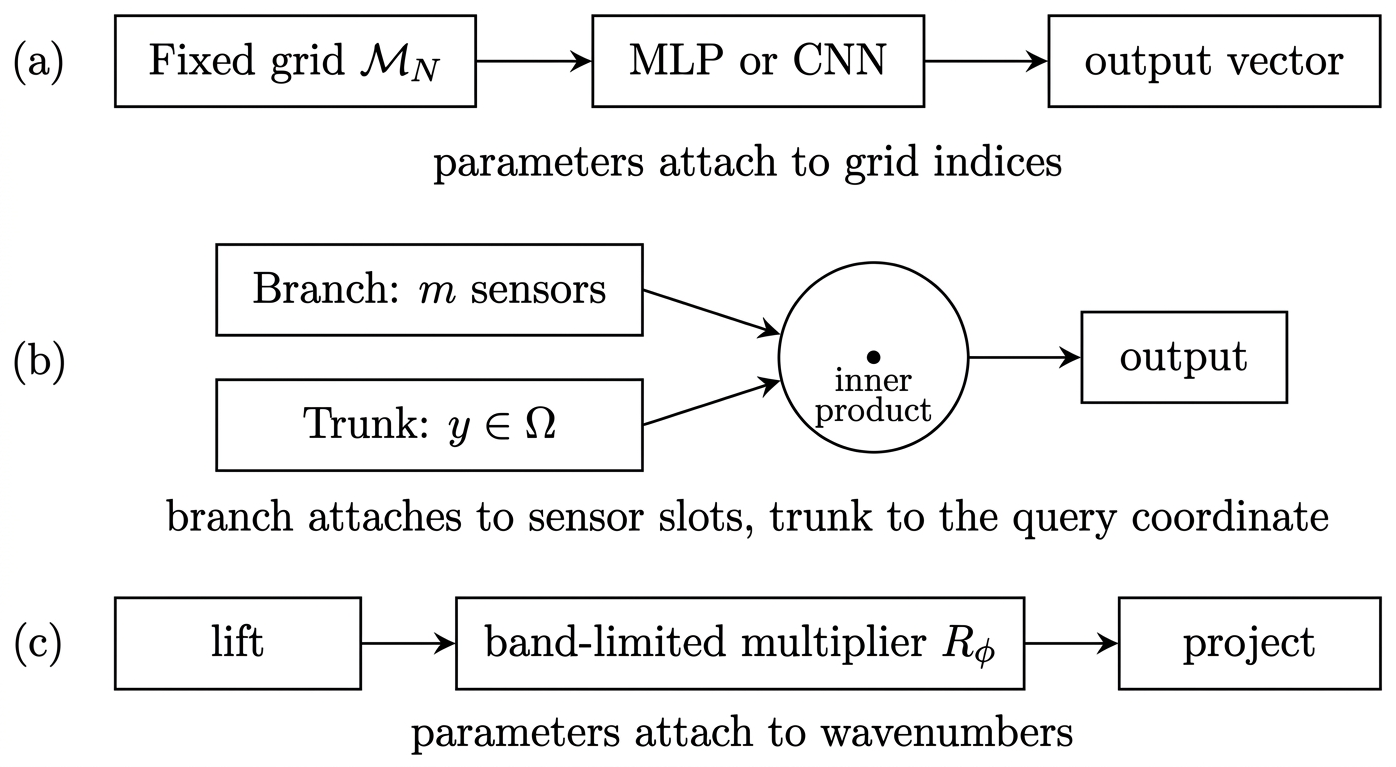
\includegraphics[width=0.82\textwidth]{fig_architectures.png}
\caption{\textbf{Three architectural families, as block diagrams.} (a) A multilayer perceptron or convolutional network consumes a vector of samples on a fixed mesh $\mathcal{M}_{N}$, so its parameters attach to grid indices. (b) DeepONet separates the two roles that \eqref{eq:chen_chen_form} couples: a branch bound to $m$ input sensors, a trunk accepting any continuous $y\in\Omega$, fused by the inner product of \eqref{eq:ch04-deeponet}. (c) The Fourier neural operator \cite{li2021fourier} keeps the lift-and-project sandwich of \eqref{eq:no_composition} but replaces the dense kernel of \eqref{eq:fredholm_kernel} with a spectral convolution, so its parameters attach to wavenumbers. Read in that order the panels isolate one axis of difference: what the parameters are functions of. The plate is a schematic rendering of the constructions defined in this chapter and carries no measured value.}
\label{fig:architectures}
\end{figure}

% -----------------------------------------------------------------------------
\section{What the Universality Theorems Do Not Say}
% -----------------------------------------------------------------------------

Put in sequence, Theorems~\ref{thm:chen_chen} and~\ref{thm:no_universality}, together with the error taxonomy of Remark~\ref{thm:deeponet_error}, deliver a reassuring conclusion: no architecture family considered here is fundamentally unable to represent a PDE solution operator. Three questions remain open, and each reappears later in the book.

The first is cost. Discretizing \eqref{eq:fredholm_kernel} on $N$ nodes forms an $N\times N$ kernel matrix, so a densely parameterized layer is $\mathcal{O}(N^{2})$ in time and memory, which is prohibitive in two and three dimensions. The contraction \eqref{eq:ch04-deeponet} carries no such bottleneck, because a rank-$p$ sum is cheap, but its expressivity is capped by the same $p$ that governs $\mathcal{E}_{\text{basis}}(p)$ in \eqref{eq:ch04-error-split}. The generic framework of~\cite{kovachki2023neural} admits several tractable kernel parameterizations in response --- graph-based, low-rank, multipole, and Fourier~\cite{li2021fourier} --- each buying efficiency by restricting the kernel's dependence on $(x,y)$, and each restriction must then earn back the accuracy it forfeits. Theorem~\ref{thm:no_universality} cannot say which restriction is worthwhile; that is an architectural question, and Part I answers it for the Fourier case.

The second is rate. An existential theorem supplies a family of approximators but no map from $\varepsilon$ to $(L,d_{v},p,m)$, so it cannot distinguish an architecture needing parameters polynomial in $1/\varepsilon$ from one needing them exponentially large --- and a surrogate whose size explodes with accuracy is useless in practice. Bounds of this kind do exist for the two architectures that dominate the rest of the book. For DeepONets, \cite{lanthaler2022error} control the three contributions in \eqref{eq:ch04-error-split} through the spectral decay of the covariance operators of the input and output measures, converting the bare requirement ``$K$ is compact'' into a computable statement about how fast the leading coefficients of the data ensemble decay. For Fourier neural operators, \cite{kovachki2021universal} prove universality together with explicit error bounds, and show that for the solution operators of Darcy flow and of the incompressible Navier--Stokes equations the network size required to reach error $\varepsilon$ grows only sub-log-linearly in $1/\varepsilon$ --- efficiency in precisely the sense the existential results above decline to provide.\index{Darcy flow!approximation}\index{Navier--Stokes equations!approximation}\index{universality!versus efficiency}\index{Fourier neural operator!error bounds}

The third is training. Every result in this chapter is a statement about a hypothesis class. None asserts that stochastic gradient descent finds a member of it, that empirical risk on a finite training set controls the supremum in \eqref{eq:ch04-unif-bound} over $K$, or that the loss landscape is benign. All three terms of \eqref{eq:ch04-error-split} are class-level quantities --- sensors, basis, network size --- and none is a statement about optimization; the gap the split omits lives outside it. This chapter has kept them apart deliberately: generalization and stability are taken up in \chapref{ch:part1-open-theoretical-problems-and-mathematical}, their empirical counterpart in Part II. What universality does accomplish is narrower and sufficient to justify everything that follows. Where the hypotheses of the three theorems hold --- a target that is continuous on a compact input set --- a neural operator that fails on a PDE family fails in the budget, the parameterization, the data, or the optimizer, not in the representability of the target. Where those hypotheses fail, as they do for a transport map that propagates a discontinuity without smoothing it, the theorems make no promise at all, and \chapref{ch:part1-open-theoretical-problems-and-mathematical} records that as an open problem rather than a solved one.\index{universality!scope of the hypotheses}

% -----------------------------------------------------------------------------
% Bridge to Chapter 5
% -----------------------------------------------------------------------------

The unresolved item from the preceding section is the cost of the nonlocal term, and it is the reason \chapref{ch:part1-the-fourier-neural-operator-spectral-theor} exists. An $\mathcal{O}(N^{2})$ kernel integral is affordable only if the kernel's dependence on $(x,y)$ is restricted, so the question becomes what to give up. A translation-invariant kernel $\kappa(x-y)$ on a periodic domain surrenders the input conditioning visible in \eqref{eq:fredholm_kernel}, but it turns the integral of \eqref{eq:fredholm_kernel} into a convolution, and convolutions are diagonal in the Fourier basis. That single observation converts dense integration into per-mode multiplication by a learnable complex matrix, evaluated in $\mathcal{O}(N\log N)$ with a fast Fourier transform (FFT), and it relocates the parameters onto wavenumbers instead of grid indices --- the structural premise of the discretization-invariance analysis in \chapref{ch:part1-discretization-invariance-and-continuum-li}.\index{discretization invariance}\index{mesh independence|see{discretization invariance}} \chapref{ch:part1-the-fourier-neural-operator-spectral-theor} develops exactly that construction: Fourier multipliers and stationary kernels, mode truncation to a finite set $Z_{k_{\max}}$, the conjugate-symmetry constraint that keeps outputs real-valued, and the spectral layer \eqref{eq:fno_layer}, which replaces the integral in \eqref{eq:no_layer}. It then supplies the rate statement this chapter withheld, splitting the error into a spectral truncation part that decays algebraically in $k_{\max}$ and a neural parametric floor --- the analogue, in a frequency parameterization, of the basis term $\mathcal{E}_{\text{basis}}(p)$ in \eqref{eq:ch04-error-split}.

% Chapter 5: The Fourier Neural Operator: Spectral Theory and Convergence
% Part I of the book.

\chapter{The Fourier Neural Operator: Spectral Theory and Convergence}
\label{ch:part1-the-fourier-neural-operator-spectral-theor}
\label{sec:fno}
% -----------------------------------------------------------------------------

\chapref{ch:part1-operator-approximation-theory-and-universa} ends on an
existence result and says nothing about price. A neural operator built from a
pointwise lift, integral kernel layers, and a pointwise projection approximates
any continuous operator on a compact input set, provided the kernel
$\kappa_\ell(x,y,a(x),a(y))$ in \eqref{eq:fredholm_kernel} is free to depend on
both arguments and on the field itself. Discretized on $N$ quadrature nodes,
that freedom costs an $N \times N$ array per layer and a dense matrix-vector
product per application. A field on a $256 \times 256$ grid is
$N \approx 6.5 \times 10^4$ unknowns, so a single layer commits $4 \times 10^9$
kernel evaluations per input, and four layers make an existence proof into
arithmetic nobody pays for.

The \textbf{Fourier Neural Operator} (FNO)~\cite{li2021fourier} escapes the
\index{Fourier neural operator}
bottleneck by accepting a restriction rather than by inventing a faster dense
product. It requires the kernel to be \emph{stationary},
$\kappa(x,y)=\kappa(x-y)$, and the domain to be the periodic torus
$\mathbb{T}^d$. Both are modeling assumptions. They declare the medium
homogeneous and the boundary periodic, and they remove
the explicit input dependence that the generic kernel carries. The premise binds
the kernel of each layer; the network as a whole is freer --- the lifted
channels and the local bypass can partially disguise a mild inhomogeneity, as
the taxonomy of
\chapref{ch:part1-comparative-theoretical-taxonomy-of-archit} argues --- but it
cannot be wished away, and Section~\ref{sec:ch05-truncation} records what it
costs. In exchange,
translation invariance diagonalizes the operator. The complex exponentials are
eigenfunctions of every stationary convolution simultaneously, so the kernel
collapses from a function of $2d$ real variables to a function of one integer
index. A grid application then costs $\mathcal{O}(N \log N)$ with the fast
Fourier transform (FFT), against $\mathcal{O}(N^2)$ for the dense product.
\index{fast Fourier transform (FFT)}
\index{periodic domain (torus)}

This chapter develops that exchange at the level of rigor Part I requires. The
first section derives the multiplier representation and states plainly what
stationarity gives up. The second truncates the multiplier to a finite mode set
and assembles the continuum layer, comparing it term by term with the generic
construction. The third states the convergence theorem, works through its
proof, and reads the resulting rate off a computed figure. The reader should
arrive with the Fourier-series characterization of $H^s(\mathbb{T}^d)$ from
\chapref{ch:part1-function-spaces-duality-and-sobolev-regula}, the smoothing
examples of \chapref{ch:part1-partial-differential-equations-as-solution}, and
the architecture of \chapref{ch:part1-operator-approximation-theory-and-universa}.
Two warnings recur and are best stated at the outset: every bound below is an
upper bound whose constants the theory does not produce, and every statement
concerns the continuum layer rather than the discrete transform a training loop
evaluates. The second warning is the subject of
\chapref{ch:part1-discretization-invariance-and-continuum-li}.

% -----------------------------------------------------------------------------
\section{Fourier Multipliers and Stationary Convolutional Kernels}
\label{sec:ch05-multipliers}

The kernel layer \eqref{eq:fredholm_kernel} is deliberately general:
$\kappa_\ell$ may depend on the source point, the target point, and the input
field at both. That generality is what makes the universality theorem true and
what makes its discretization dense. The FNO surrenders the first two
dependencies at once. It works on the flat torus
$\mathbb{T}^d \cong [0,1)^d$ of
\chapref{ch:part1-function-spaces-duality-and-sobolev-regula} and assumes a
\textbf{stationary kernel}, a function of the separation alone, so that
substituting $\kappa(x,y) = \kappa(x-y)$ into \eqref{eq:fredholm_kernel} turns
the integral into a convolution on a compact abelian group:
\index{stationary kernel}
\index{translation-invariant kernel}
\index{convolution!on the torus}
\begin{equation}
  \label{eq:ch05-convolution}
  (\mathcal{K} v)(x) = \int_{\mathbb{T}^d} \kappa(x - y) v(y) \, dy = (\kappa * v)(x).
\end{equation}
For $\kappa, v \in L^2(\mathbb{T}^d)$ the integrand is integrable by
Cauchy--Schwarz, so \eqref{eq:ch05-convolution} is defined pointwise, and
Young's inequality on the torus upgrades it to a bounded function; when either
factor is smoother, the convolution inherits that smoothness.

The reason the restriction pays is that the Fourier basis diagonalizes every
stationary operator at once. Write the coefficients with the convention of
\chapref{ch:part1-function-spaces-duality-and-sobolev-regula},
$\hat{u}(k) = \int_{\mathbb{T}^d} u(x) e^{-2\pi i k \cdot x}\,dx$, so that
$u(x) = \sum_{k} \hat{u}(k) e^{2\pi i k \cdot x}$. For the exponential
$e_k(x) = e^{2\pi i k \cdot x}$ the change of variables $z = x - y$ gives
$(\kappa * e_k)(x) = e^{2\pi i k \cdot x} \int_{\mathbb{T}^d} \kappa(z)
e^{-2\pi i k \cdot z}\,dz = \hat{\kappa}(k)\, e_k(x)$. The exponentials are
eigenfunctions of \emph{all} such convolutions simultaneously, and the
eigenvalue attached to mode $k$ is precisely the $k$-th Fourier coefficient of
the kernel. Stated as an identity on coefficients, this is the convolution
theorem for Fourier series:
\index{convolution theorem}
\index{Fourier multiplier}
\begin{equation}
  \label{eq:ch05-convolution-theorem}
  \mathcal{F}(\kappa * v)(k) = \mathcal{F}(\kappa)(k) \cdot \mathcal{F}(v)(k) = \hat{\kappa}(k) \, \hat{v}(k), \quad k \in \mathbb{Z}^d.
\end{equation}

Equation \eqref{eq:ch05-convolution-theorem} is the entire computational
argument. An operator that mixed modes would need a matrix indexed by pairs of
frequencies; a stationary one needs a single sequence, and \eqref{eq:ch05-convolution-theorem}
shows the sequence is nothing but the kernel's own spectrum. Read the other
way, the same identity says exactly what has been given up: if $\kappa$ depends
on $x$ and $y$ separately, $\mathcal{K}$ scatters energy among modes and no
diagonal object represents it. Stationarity is a claim about the physics
--- homogeneous medium, no distinguished location, periodic boundary --- and a
learned filter on, say, a bounded domain with boundary layers either has to
disguise the inhomogeneity or hand it to another component.

Rather than parameterizing $\kappa(x-y)$ in physical space and integrating
numerically, the FNO parameterizes the multiplier directly. The hidden field
$v_\ell$ takes values in $\mathbb{R}^{d_v}$, so the multiplier is
matrix-valued:
\index{channel mixing}
\index{Fourier multiplier $R_\phi(k)$}
\begin{equation}
  \label{eq:ch05-multiplier}
  R_\phi(k) \in \mathbb{C}^{d_v \times d_v}, \quad k \in \mathbb{Z}^d,
\end{equation}
with $\phi$ collecting all retained entries into one parameter vector. At mode
$k$ the layer multiplies the channel vector $\hat{v}(k) \in \mathbb{C}^{d_v}$ by
$R_\phi(k)$, so channels mix \emph{inside} a frequency and never \emph{across}
frequencies. The physical kernel is recoverable from
$R_\phi$ by the inverse transform,
$\kappa(x) = \sum_{k} R_\phi(k) e^{2\pi i k \cdot x}$, which is the precise
sense in which learning a multiplier is learning a convolution kernel: the two
are the same object written in two coordinate systems. Restricting
$R_\phi(k)$ to be diagonal would cut the per-mode parameter count from $d_v^2$
to $d_v$ at the cost of forbidding channel mixing; \eqref{eq:ch05-multiplier}
keeps the general matrix, and the mode-budget analysis of
Section~\ref{sec:ch05-rates} is indifferent to that choice, since it constrains
how many $k$ carry weight rather than what each $d_v \times d_v$ block looks
like.

The cost is worth tallying before moving on. On a grid of $N$ points in total,
one layer costs two transforms, $\mathcal{O}(d_v N \log N)$, plus one
matrix-vector product per retained mode, $\mathcal{O}(|Z_{k_{\max}}| d_v^2)$,
where $Z_{k_{\max}}$ is the mode set introduced in \eqref{eq:ch05-modeset}
below. Because $|Z_{k_{\max}}|$ is fixed by design, the learned part of the
computation stops growing with resolution: only the transforms scale, and they
scale near-linearly rather than quadratically~\cite{kovachki2023neural}. This
is the $\mathcal{O}(N \log N)$ entry recorded for the FNO in the architectural
comparison of \chapref{ch:part1-comparative-theoretical-taxonomy-of-archit},
whose per-layer count $\Theta(d_v N \log N + K d_v^{2})$ in
\eqref{eq:ch8-costs} is the same tally with $K = |Z_{k_{\max}}|$; that chapter
also notes the premise the tally is bought with.
\index{Fourier neural operator!computational cost}

\begin{remark}[Stability of a single spectral layer]
\label{rem:ch05-lipschitz}
Because \eqref{eq:ch05-convolution-theorem} couples no modes, Parseval's
identity makes the operator norm of the spectral branch explicit:
\index{Parseval identity}
$\|\mathcal{K} v\|_{L^2(\mathbb{T}^d)}^2 = \sum_{k} \|R_\phi(k)\hat{v}(k)\|_{\mathbb{C}^{d_v}}^2
\le \big(\sup_{k}\|R_\phi(k)\|_{\mathrm{op}}\big)^2 \|v\|_{L^2}^2$.
Combining this with $\|W_\ell v\|_{L^2} \le \|W_\ell\|_{\mathrm{op}}\|v\|_{L^2}$
and an elementwise $L_\sigma$-Lipschitz activation, the bias term cancels in
differences and the layer \eqref{eq:fno_layer} is Lipschitz with constant
$L_\sigma\big(\|W_\ell\|_{\mathrm{op}} + \sup_k \|R_\phi(k)\|_{\mathrm{op}}\big)$.
A trained FNO is therefore continuous by construction, which is the hypothesis
every approximation result in this part needs, and the certificate is a maximum
of singular values across modes --- a property of the parameters, not of the
data.
\end{remark}

% -----------------------------------------------------------------------------
\section{Spectral Truncation and Mathematical Formulation}
\label{sec:ch05-truncation}

A multiplier on all of $\mathbb{Z}^d$ is infinitely many parameters, so it must
be cut, and regularity is what licenses the cut. If $v \in H^s(\mathbb{T}^d)$
with $s > 0$, then every term in the weighted $\ell^2$ sum defining
$\|v\|_{H^s}$ is non-negative, whence
$(1+|k|^2)^{s/2}|\hat{v}(k)| \le \|v\|_{H^s}$ for each $k$ individually. That
pointwise bound is the estimate the architecture depends on:
\index{Sobolev space!Fourier coefficient decay}
\begin{equation}
  \label{eq:ch05-coefficient-decay}
  |\hat{v}(k)| \le \frac{C}{\big(1 + |k|^2\big)^{s/2}} \|v\|_{H^s},
\end{equation}
where the constant $C$ is carried along so that the display covers equivalent
norm conventions. Note what \eqref{eq:ch05-coefficient-decay} does and does not
say. It gives algebraic decay, $|\hat{v}(k)| = O(|k|^{-s})$, not exponential
decay; and it is a statement per coefficient, whereas truncation errors are
$\ell^2$ tail quantities. Both features resurface in the rate of
Theorem~\ref{thm:fno_convergence}.

The retained set is
\index{spectral truncation}
\index{mode set $Z_{k_{\max}}$}
\begin{equation}
  \label{eq:ch05-modeset}
  Z_{k_{\max}} = \left\{ k = (k_1, \dots, k_d) \in \mathbb{Z}^d : |k_j| \le k_{\max, j}, \quad j = 1, \dots, d \right\}.
\end{equation}
A box rather than the ball $\{|k|\le k_{\max}\}$, for one practical reason:
\eqref{eq:ch05-modeset} is a product of contiguous index ranges, which is what
a batched transform can slice without gathering scattered entries --- Part
II's spectral convolution keeps the two low corners of the half-spectrum along
the first axis for exactly this reason (\chapref{ch:part2-fourier-neural-operators-fno-from-scratch}).
Counting is then immediate: \eqref{eq:ch05-modeset} holds
$\textstyle|Z_{k_{\max}}| = \prod_{j=1}^d (2k_{\max,j}+1)$ modes, so a layer
carries one complex $d_v \times d_v$ matrix per mode --- $2\,d_v^2
|Z_{k_{\max}}|$ real numbers before any symmetry is imposed --- plus $d_v^2$ in
the local matrix $W_\ell$. The conjugacy condition \eqref{eq:ch05-reality} below
roughly halves the first count, since the block at $-k$ then stores nothing the
block at $k$ does not; only the self-conjugate indices, whose blocks are real,
contribute on their own. Tail rates for the box and the ball
differ only in how the remainder is ordered, not in the power of
$k_{\max}$ that appears.

With $R_{\phi,\ell}$ understood to vanish off $Z_{k_{\max}}$, the continuum FNO
layer is
\index{Fourier neural operator!layer definition}
\begin{equation}
  \label{eq:fno_layer}
  v_{\ell+1}(x) = \sigma\left( W_\ell v_\ell(x) + \mathcal{F}^{-1}\Big( R_{\phi, \ell}(k) \cdot (\mathcal{F} v_\ell)(k) \Big)(x) + b_\ell(x) \right),
\end{equation}
and the four ingredients differ in how they act. Here
$\mathcal{F}$ and $\mathcal{F}^{-1}$ are the continuous Fourier transform and
its inverse on $\mathbb{T}^d$; $R_{\phi,\ell} : Z_{k_{\max}} \to
\mathbb{C}^{d_v \times d_v}$ is the learned complex tensor acting on the
channel vector at each retained mode $k \in Z_{k_{\max}}$ and identically zero
for $k \notin Z_{k_{\max}}$, which is how truncation enters the formula;
$W_\ell$ and $b_\ell$ carry the pointwise local part; and $\sigma$ acts
channelwise. Compare \eqref{eq:no_layer} term by term and the relationship is
plain: same local linear map, same non-local integral term with the Fredholm
kernel replaced by the band-limited multiplier of
\eqref{eq:ch05-multiplier}, same bias and activation, and the same global
composition $\mathcal{G}_\theta = \mathcal{Q}\circ\mathcal{V}_L\circ\cdots\circ\mathcal{V}_1\circ\mathcal{P}$
of \eqref{eq:no_composition}. The FNO is a special case of the generic neural
operator, not a competing design.

Being a special case, however, does not make it universal by inheritance.
Stationary band-limited kernels form a thin subclass of all continuous kernels
on $\Omega \times \Omega$, so the density argument of
\chapref{ch:part1-operator-approximation-theory-and-universa} has to be
redone with the truncation visible. It has been: universal approximation for
the FNO architecture itself, with the error expressed through the decay of the
target operator's Fourier coefficients, is established
in~\cite{kovachki2021universal}, and the quantitative version for smoothing
solution operators is the theorem of the next section.

One constraint on $R_\phi$ remains. Nothing in \eqref{eq:fno_layer} yet forces
a real-valued output from a real-valued input. Because $v_\ell$ is real, its
coefficients satisfy $\hat{v}_\ell(-k) = \overline{\hat{v}_\ell(k)}$, and
requiring the same of $v_{\ell+1}$ for every admissible input forces
\index{conjugate symmetry!of spectral weights}
\begin{equation}
  \label{eq:ch05-reality}
  R_\phi(-k) = \overline{R_\phi(k)} \quad \forall k \in Z_{k_{\max}}.
\end{equation}
The condition is an entrywise conjugacy, not a Hermitian symmetry: no transpose
appears, because \eqref{eq:ch05-reality} must hold after multiplication by an
arbitrary coefficient vector $\hat{v}(k)$. Self-conjugate indices --- $k = 0$,
and on an even grid the Nyquist index, whose partner coincides with it --- have
no separate counterpart, and their multipliers are real. Implementations do not
enforce \eqref{eq:ch05-reality} on a full-spectrum tensor by hand. They store
weights for half of the modes and let the inverse real transform reconstruct
the conjugate half, so the symmetry holds by construction; that is the origin of
the two paired weight tensors of
\chapref{ch:part2-fourier-neural-operators-fno-from-scratch}.

The cost of truncation should be stated as plainly as the benefit. A
\index{band-limited input}
band-limited branch represents nothing outside $Z_{k_{\max}}$, and the local
branch $W_\ell$ is pointwise, so it cannot relocate information globally either.
When the target has genuinely high-frequency content the estimate
\eqref{eq:ch05-coefficient-decay} degrades with the regularity actually
available: as viscosity tends to zero in Burgers' equation, steep gradients and
\index{Burgers' equation!breakdown of spectral truncation}
shocks transfer energy to arbitrarily large $|k|$
(\chapref{ch:part1-partial-differential-equations-as-solution}), and a spectral
representation additionally rings near jumps rather than resolving them --- the
\index{Gibbs phenomenon}
Gibbs phenomenon, recorded among the open problems of
\chapref{ch:part1-open-theoretical-problems-and-mathematical}. Within the band,
however, the approximation is not heuristic, and that is the regime the next
section quantifies.

% -----------------------------------------------------------------------------
\section{Spectral Error Bounds and Convergence Rates}
\label{sec:ch05-rates}

Two questions remain about \eqref{eq:fno_layer}. How much error does the
truncation in \eqref{eq:ch05-modeset} commit, and how much do the finite depth
and width add? The answer is a sum of two algebraically controlled terms, and
its shape matters more than its constants. The hypotheses deserve attention
before the statement: $\alpha > 0$ says the target gains derivatives, which
holds for the parabolic and elliptic problems of
\chapref{ch:part1-partial-differential-equations-as-solution} --- the periodic
heat semigroup gains regularity of every order, while the Darcy solution
operator of
\index{Darcy flow!regularity gain}
\eqref{eq:darcy} buys the regularity its energy estimate provides and sends
bounded coefficient sets into a bounded subset of $H^1_0$; \eqref{eq:darcy} is
posed there on a bounded domain with homogeneous Dirichlet conditions, and on
the torus the same estimate reads in the homogeneous seminorm, which is the
form the theorem speaks of. $K$ is assumed
compact. This follows the source: the error bounds of Kovachki, Lanthaler, and
Mishra~\cite{kovachki2021universal} quantify over compact sets, and
\chapref{ch:part1-function-spaces-duality-and-sobolev-regula} warned that on
bounded-but-not-compact sets the hypotheses of such theorems simply are not met.
Composed with the smoothing, compactness of $K$ makes $\mathcal{G}(K)$ compact
in $H^{s+\alpha}$ and hence precompact in $H^s$ through the Rellich--Kondrachov
embedding of
\chapref{ch:part1-function-spaces-duality-and-sobolev-regula}, which is
precisely the condition under which continuity becomes uniform approximation,
and it supplies the bound $M := \sup_{u \in K} \|\mathcal{G}(u)\|_{H^{s+\alpha}}
< \infty$ that the proof consumes.
The statement below restates their spectral convergence theorem in this book's
notation with the two error sources displayed separately.

\begin{theorem}[FNO Spectral Convergence Bound]
\label{thm:fno_convergence}
Let $\mathcal{G} : H^s(\mathbb{T}^d; \mathbb{R}^{d_a}) \to H^{s+\alpha}(\mathbb{T}^d; \mathbb{R}^{d_u})$ be a continuous nonlinear solution operator with smoothing order $\alpha > 0$, and let $K \subset H^s(\mathbb{T}^d)$ be a compact set.

Write $\Theta(L, d_v, k_{\max})$ for the class of FNO networks of depth $L$, width $d_v$, whose multiplier $R_{\phi}$ is parameterized up to wavenumber $k_{\max}$ in each spatial dimension, and set
\begin{equation}
  \label{eq:ch05-enn-def}
  \mathcal{E}_{\text{NN}}(L, d_v) := \inf_{\theta \in \Theta(L, d_v, k_{\max})} \; \sup_{u \in K} \big\| P_{k_{\max}} \mathcal{G}(u) - \mathcal{G}_\theta(u) \big\|_{L^2(\mathbb{T}^d)},
\end{equation}
the error of the best member of the class at representing the band-limited target, where $P_{k_{\max}}$ is the projection defined in the proof below. Then the approximation error of the best network in the class decomposes as:
\index{FNO spectral convergence bound}
\index{smoothing order}
\begin{equation}
  \label{eq:ch05-error-decomposition}
  \inf_{\theta \in \Theta} \sup_{u \in K} \|\mathcal{G}(u) - \mathcal{G}_\theta(u)\|_{L^2} \le \underbrace{C_1 \, k_{\max}^{-(s+\alpha)}}_{\text{Spectral Truncation}} + \underbrace{\mathcal{E}_{\text{NN}}(L, d_v)}_{\text{Neural Parametric Error}},
\end{equation}
where $C_1$ depends on $d$, $s$, $\alpha$ and on $M = \sup_{u \in K} \|\mathcal{G}(u)\|_{H^{s+\alpha}}$, and $\mathcal{E}_{\text{NN}}$ on the class sizes $L$, $d_v$, $k_{\max}$; nothing in the display depends on a deployment grid, and the distance between the best network and the one a training loop returns lies outside it entirely.
\end{theorem}

\begin{proof}[Justification of the truncation term]
Let $P_{k_{\max}}$ denote the $L^2$-orthogonal projection onto the subspace spanned by Fourier modes in $Z_{k_{\max}}$:
\index{orthogonal projection!Fourier partial sum}
\begin{equation}
  \label{eq:ch05-projection}
  (P_{k_{\max}} w)(x) = \sum_{k \in Z_{k_{\max}}} \hat{w}(k) e^{2\pi i k \cdot x}.
\end{equation}
For any function $w \in H^{s+\alpha}(\mathbb{T}^d)$, the projection error satisfies:
\begin{equation}
  \label{eq:ch05-projection-bound}
  \begin{aligned}
    \|w - P_{k_{\max}} w\|_{L^2}^2 = \sum_{k \notin Z_{k_{\max}}} |\hat{w}(k)|^2
    &\le \frac{1}{(1 + k_{\max}^2)^{s+\alpha}} \sum_{k \notin Z_{k_{\max}}} (1 + |k|^2)^{s+\alpha} |\hat{w}(k)|^2 \\
    &\le \frac{1}{(1 + k_{\max}^2)^{s+\alpha}} \|w\|_{H^{s+\alpha}}^2.
  \end{aligned}
\end{equation}
The middle step uses $|k| \ge \max_i |k_i| > k_{\max}$ for every discarded mode $k \notin Z_{k_{\max}}$.
Taking the square root and writing $M$ for the bound on $\|w\|_{H^{s+\alpha}}$ yields $\|w - P_{k_{\max}} w\|_{L^2} \le C M k_{\max}^{-(s+\alpha)}$, and applying this to every $w$ in $\mathcal{G}(K)$ bounds the truncation term uniformly over $K$. The remaining component $\mathcal{E}_{\text{NN}}$ arises from approximating the finite collection of complex multiplier matrices $\{R(k)\}_{k \in Z_{k_{\max}}}$ and local transformations using feedforward layers.
\end{proof}

One exponent deserves care, because an earlier drafting of this chapter
printed the wrong one. The truncation term in
\eqref{eq:ch05-error-decomposition} decays as $k_{\max}^{-(s+\alpha)}$: the
exponent is the \emph{output} regularity $s + \alpha$ of the target, not the
operator's gain $\alpha$ alone, since what is truncated is the tail of
$\mathcal{G}(u)$, a function of $s+\alpha$ derivatives in $L^2$. A weaker
$k_{\max}^{-\alpha}$ bound follows for $k_{\max} \ge 1$, but it is a deliberate
degradation, not a constant absorbed into $C_1$: no constant can move an
exponent. What downstream chapters must carry --- at a shock, at a front, in
the taxonomy ledger --- is the regularity of the output, which the smoothing
hypothesis bounds by $s + \alpha$ and which a discontinuity drives below $1/2$
outright. Also worth noting: the sum in \eqref{eq:ch05-projection-bound} now
runs over the complement of the box \eqref{eq:ch05-modeset}, exactly the modes
the projector discards; the round-tail set written there in the earlier drafting
was not the discarded set, and the estimate survived only because the mistaken
inclusion ran in the favorable direction.

The second term, $\mathcal{E}_{\text{NN}}(L,d_v)$, is
\index{neural parametric error}
the error of representing the finitely many matrices
$\{R(k)\}_{k \in Z_{k_{\max}}}$ and the local maps within a network of depth
$L$ and width $d_v$; it is an approximation-theoretic quantity, and
\eqref{eq:ch05-error-decomposition} asserts it can be made small, not how fast.
That it can be made small at all is a density fact about the class, established
in \chapref{ch:part1-operator-approximation-theory-and-universa};
Remark~\ref{rem:ch05-lipschitz} grants each member of the class Lipschitz
continuity --- a property of the networks, not a rate for the infimum.
Nor does the bound say anything about training: \eqref{eq:ch05-enn-def} prices
the best parameters, and the gap between them and the parameters a solver
returns is outside the display.
A more informative split
for a learned surrogate is the three-way decomposition proved for Fourier
\index{error decomposition!statistical, discretization, and truncation}
linear operators by Subedi and Tewari~\cite{subedi2024controlling}, who
separate a \emph{statistical} term, decaying with the number of training
input-output pairs, a \emph{discretization} term, controlled by the grid
spacing at which the field is sampled, and a \emph{truncation} term from
\index{truncation error!algebraic rate}
keeping finitely many modes. Theorem~\ref{thm:fno_convergence} prices only the third of these, through $C_1
k_{\max}^{-(s+\alpha)}$; its $\mathcal{E}_{\text{NN}}$ is data-free, so the statistical term is not
folded in but absent, and the discretization term is suppressed altogether, because the
theorem is a statement about continuum layers. The decay rate behind the truncation term is
easy to see in a model, and the model is the one drawn in
Figure~\ref{fig:spectral_decay}. Let $\tau$ denote a coefficient decay
exponent --- the letter is reserved here precisely so that $\sigma$ can keep
meaning the activation --- and suppose $|\hat{w}(k)| \lesssim |k|^{-\tau}$ with
$\tau > d/2$, so that the tail discarded by the projection
\eqref{eq:ch05-projection} is square summable. Then the squared tail behaves
like
$\sum_{|k| > k_{\max}} |k|^{-2\tau} \approx \int_{k_{\max}}^\infty
r^{d-1-2\tau}\,\mathrm{d}r$, so $\|(I - P_{k_{\max}})w\|_{L^2} =
O\big(k_{\max}^{-(\tau - d/2)}\big)$. The half order lost per dimension is mode
bookkeeping rather than a property of the field: the factor
$r^{d-1}\,\mathrm{d}r$ counts the lattice points in the shell being emptied.
With $\tau = s$ in one dimension this is exactly the slope
$-(s - \tfrac12)$ computed in Figure~\ref{fig:spectral_decay}(b).

\begin{figure}[htbp]
\centering
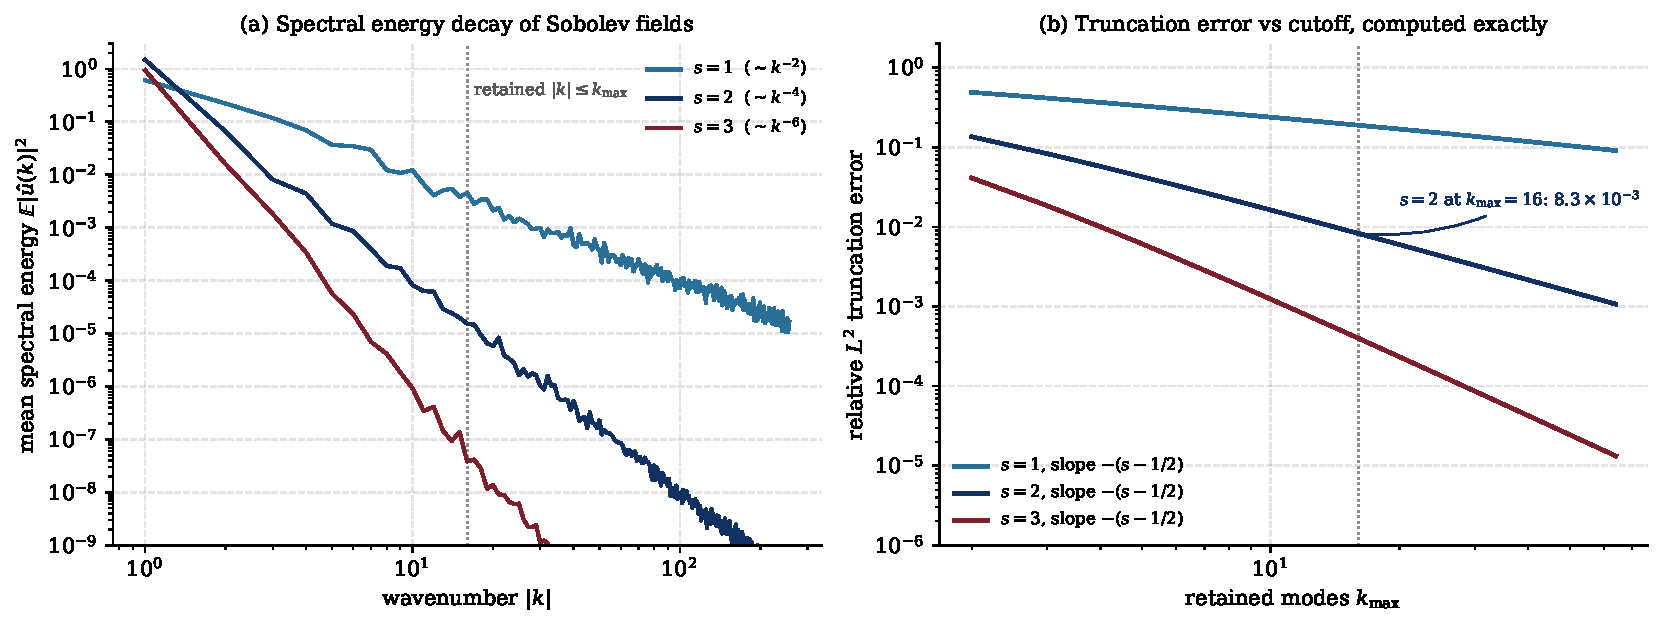
\includegraphics[width=0.88\textwidth]{fig_spectral_decay.pdf}
\caption{\textbf{Spectral decay and the cost of truncation, computed rather than drawn schematically.} Both panels use the Sobolev model $\hat{u}(k) = |k|^{-s}\xi_k$ with $\xi_k$ independent standard normal and $s \in \{1,2,3\}$. (a) Mean spectral energy $\mathbb{E}|\hat{u}(k)|^2 = k^{-2s}$, averaged over 40 draws, with the dotted vertical line marking a retained band $|k| \le k_{\max} = 16$. (b) Exactly computed relative $L^2$ error of the band projection $P_{k_{\max}}$ of \eqref{eq:ch05-projection}, namely $\|(I-P_{k_{\max}})u\|_{L^2}/\|u\|_{L^2} = \big(\sum_{k_{\max}<k\le 512} k^{-2s} \big/ \sum_{1\le k\le 512} k^{-2s}\big)^{1/2}$ on a grid resolving $|k| \le 512$, for $k_{\max} = 2,\dots,64$; the log-log slope is $-(s-\tfrac12)$, as marked. Panel (b) isolates truncation: no horizontal line is drawn, because the neural term of \eqref{eq:ch05-error-decomposition} is measured for exactly one
architecture in this book, the worked example of Appendix~\ref{app:b}, and its value belongs in
that appendix rather than on this axis. The dotted vertical line marks an illustrative cutoff, $k_{\max}=16$; the worked example of Appendix~\ref{app:b} retains $k_{\max}=11$. That example is the one-dimensional periodic heat equation $u_t = \alpha u_{xx}$ with $\alpha = 0.01$ at $T = 1$, trained on inputs $u_0(x) = \sum_{k=1}^{8} c_k k^{-3/2}\cos(2\pi k x + \phi_k)$ with $c_k \sim \mathcal{N}(0,1)$ and $\phi_k$ uniform on $[0,2\pi)$, whose exact solution is $u(x,T) = \mathcal{F}^{-1}\!\big[\hat{u}_0(k)\,e^{-\alpha(2\pi k)^2 T}\big]$. The callout is the computed value at $k_{\max}=16$ for $s=2$, $8.3\times10^{-3}$, at the same cutoff drawn in panel (a). A curve that has fallen far below it is not thereby accurate --- only no longer limited by truncation.}
\label{fig:spectral_decay}
\end{figure}

Figure~\ref{fig:spectral_decay} is what a practitioner should take from
Theorem~\ref{thm:fno_convergence}. Panel (a) shows the energy bookkeeping that
makes \eqref{eq:ch05-modeset} defensible: the tail beyond a moderate cutoff
carries a small and rapidly shrinking share of the total, and the share shrinks
faster the larger the regularity $s$, which is \eqref{eq:ch05-coefficient-decay}
summed in $\ell^2$. Panel (b) converts that bookkeeping into the accuracy the
reader can expect from the first term of \eqref{eq:ch05-error-decomposition}.
Doubling $k_{\max}$ divides the relative truncation error by the asymptotic
factor $2^{\,s-1/2}$ --- $1.4$ at $s=1$, $2.8$ at $s=2$, $5.7$ at $s=3$ --- and
the computed curves come close to it: between the cutoffs $k_{\max} = 32$ and
$k_{\max} = 64$ the observed factors are $1.46$, $2.80$ and $5.55$. At the band
$k_{\max} = 16$ drawn in panel (a), the computed error is $8.3\times10^{-3}$ for
$s=2$, against $1.9\times10^{-1}$ at $s=1$, which has fallen only to
$9.1\times10^{-2}$ by the largest cutoff plotted. At one band the two curves are a
factor of $23$ apart, and what separates them is regularity. Two conclusions
follow. Once the algebraic curve has fallen below the
network's own term, adding modes buys nothing: the second term of
\eqref{eq:ch05-error-decomposition} dominates, and where that crossing sits is a
property of a particular training run. That is why the
one-dimensional example of Appendix~\ref{app:b} and the two-dimensional
reference configuration of \chapref{ch:part2-fourier-neural-operators-fno-from-scratch}
keep of order a dozen to sixteen modes per direction, not hundreds. And a
target with only one derivative is not rescued by any affordable mode budget:
regularity, not resolution, is the binding constraint.

The model problem in the caption also marks the boundary of the argument's
honesty. Heat diffusion multiplies mode $k$ by $e^{-\alpha(2\pi k)^2 T}$, which
at $\alpha = 0.01$, $T = 1$ is $1.1\times10^{-11}$ already at $k = 8$: the
solution operator smooths far faster than any power, so its truncation term is
negligible and the observed error is entirely $\mathcal{E}_{\text{NN}}$. That is
a property of the example, not a general guarantee, and the linear heat equation
is an easy case for any classical solver; the surrogate there is a teaching
device. The bound \eqref{eq:ch05-error-decomposition} earns its keep on
nonlinear targets that smooth without being analytic, and it weakens exactly
where the hypothesis of Theorem~\ref{thm:fno_convergence} fails.
\index{heat equation!spectral damping of the solution operator}

\takeaway{What the Mode Budget Buys}{For a target gaining $\alpha$ derivatives,
the truncation term of \eqref{eq:ch05-error-decomposition} is algebraic in
$k_{\max}$ and independent of depth, width, and grid; the capacity term
$\mathcal{E}_{\text{NN}}(L,d_v)$ is the part the theory can drive small but not
rate. The two set each other's useful range, and nothing in the bound connects
either of them to sample size or to the optimizer.}

\medskip
Where the argument stops, the next chapter begins.
Theorem~\ref{thm:fno_convergence} bounds the distance between a target operator
and a continuum FNO whose layer \eqref{eq:fno_layer} is written with continuous
transforms $\mathcal{F}$, $\mathcal{F}^{-1}$; a real network never computes
those. It evaluates coefficient sums on $N$ grid points, where the FFT replaces
$\mathcal{F}$ with a discrete transform whose coefficients are quadrature
approximations carrying aliasing of their own. Nothing in
\eqref{eq:ch05-error-decomposition} mentions a grid --- and that is the whole
point of the chapter that follows. The theorem bounds a continuum object, so
what still requires proof is a commutation of limits, not a property of $C_1$
or of $\mathcal{E}_{\text{NN}}$: that the discrete operator induced by any grid
converges to the continuum operator as $h \to 0$, and that the parameter vector
$\phi$ means the same object on every grid. \chapref{ch:part1-discretization-invariance-and-continuum-li} states that
property precisely, checks it for the spectral layer against the quadrature
consistency of the generic kernel, and shows why a conventional convolutional
network fails the same test --- with a consequence, zero-shot evaluation on
finer grids, that follows from the fixed band \eqref{eq:ch05-modeset} as soon as
the input is resolved on the training grid.

% Chapter 6: Discretization Invariance and Continuum Limits
% Part I of the book.

\chapter{Discretization Invariance and Continuum Limits}
\label{ch:part1-discretization-invariance-and-continuum-li}
\label{sec:discretization}
% -----------------------------------------------------------------------------

Every number a neural operator returns is computed on a grid, yet the
architecture itself is defined on function spaces.
Reconciling those two facts is the task of this chapter. Discretization
invariance\index{discretization invariance} is the property most often advertised for neural operators and the
most often overstated: it is casually read as meaning that a trained network is
accurate at any resolution, that mesh refinement costs nothing, and that the
implemented network simply \emph{is} the continuum operator. None of that
follows from the architecture alone. What does follow is narrower and
considerably more useful. A neural operator's parameters are indexed by
functions --- a kernel $\kappa(x,y)$, a multiplier $R_\phi(k)$
--- rather than by positions in an array, so one trained weight vector can be applied to
samples of the same physical field taken on different meshes; and the gap
between the resulting discrete output and the continuum output is a consistency
error that vanishes as the mesh is refined, at a rate governed by the regularity
of the fields that pass through the network.

Making that statement precise requires three ingredients the earlier chapters
supply. From \chapref{ch:part1-function-spaces-duality-and-sobolev-regula} we
need the periodic Sobolev scale $H^s(\mathbb{T}^d)$ and its embedding threshold
$s>d/2$, below which point values of an $L^2$ function do not exist and sampling
is not even defined. From
\chapref{ch:part1-operator-approximation-theory-and-universa} we need the
generic layer \eqref{eq:fredholm_kernel}, whose integral must be replaced by a
quadrature sum on any real mesh. From
\chapref{ch:part1-the-fourier-neural-operator-spectral-theor} we need the
Fourier neural operator (FNO) layer \eqref{eq:fno_layer}, the retained-mode set
$Z_{k_{\max}}$, and the
two-term bound of Theorem~\ref{thm:fno_convergence}, which accounts for spectral
truncation and neural parametrization but not for the grid. This chapter adds the
term that bound leaves out --- the error the grid itself contributes --- and
separates what is provable from what is merely
reported.

The route is as follows. We state invariance as a commutative diagram with its
hypotheses exposed, then test it where it is weakest, at the quadrature level of
integral kernels, and contrast mesh-independent operator parameters with the
pixel-indexed stencils of convolutional networks --- the point at which the
usual motivation for operator architectures becomes a calculation. An exact
transfer identity for a band-limited single spectral layer follows, together
with a reading of what a reported
``zero-shot super-resolution'' experiment does
and does not establish. The chapter ends with the algebraic continuum-limit
rate \eqref{eq:ch06-rate} for the grid error, whose mechanism is the aliasing
identity \eqref{eq:ch06-alias}, and with the
statistical--truncation--discretization decomposition of Subedi and Tewari,
which price the error a user actually pays. In the argument of Part~I this
closes the approximation theory of
\chapref{ch:part1-operator-approximation-theory-and-universa} and
\chapref{ch:part1-the-fourier-neural-operator-spectral-theor} by separating what
the architecture guarantees from what experiments show, and it hands the
currency it establishes --- regularity --- to
\chapref{ch:part1-physics-informed-operators-and-sobolev-reg}.

\section{Formal Definition of Discretization Invariance}
\label{sec:ch06-definition}

Let $\mathcal{M}_N = \{x_j^{(N)}\}_{j=1}^N \subset \Omega$ denote a spatial
discretization of the domain $\Omega$ with mesh parameter
$h_N = \sup_{x \in \Omega} \min_{x_j \in \mathcal{M}_N} \|x - x_j\|$, the
\emph{fill distance}\index{fill distance@fill distance (mesh parameter $h_N$)} of
the node set: every point of the domain lies within $h_N$ of some node. The
integer $N$ is never used here as an abstract array size. It stands for a
sequence of meshes with $h_N \to 0$, and the statements below are claimed along
such a sequence rather than for one privileged discretization.

Two operators tie the continuum to the discrete, and their roles are worth
naming before the definition is written. The \textbf{restriction} (sampling)
operator $P_N : \mathcal{A}(\Omega) \to \mathbb{R}^{N \times d_a}$, defined by
$(P_N u)_j = u(x_j^{(N)})$ \index{restriction operator@restriction operator $P_N$},
turns a function into the array a computer sees; here $d_a$ and $d_u$ are the
input and output channel counts of
\chapref{ch:part1-operator-approximation-theory-and-universa}. The
\textbf{extension}
(interpolation) operator $I_N : \mathbb{R}^{N \times d_u} \to \mathcal{U}(\Omega)$
\index{extension operator@extension operator $I_N$}
does the reverse and is required only to be asymptotically lossless:
$\lim_{N \to \infty} \|I_N P_N u - u\|_{\mathcal{U}} = 0$ for every $u$ in a
dense subspace of $\mathcal{U}$. Concrete choices abound --- piecewise-linear
Lagrange interpolation, cell-average reconstruction, trigonometric polynomial
interpolation --- and the definition is deliberately agnostic among them,
because the interesting question is which reconstruction an architecture makes
natural. For spectral layers it is the trigonometric interpolant, as the
argument of Proposition~\ref{prop:ch06-zeroshot} shows. The formulation below is
the condition imposed on neural operators in \cite{kovachki2023neural}.

\begin{definition}[Discretization Invariance]
\label{def:ch06-discretization-invariance}
\index{discretization invariance!formal definition}
An architecture family $\{\mathcal{G}_\theta\}_{\theta \in \Theta}$ is
\textbf{discretization-invariant} if three conditions hold. \emph{(i)} The
parameter space $\Theta$ is defined independently of any specific mesh
$\mathcal{M}_N$. \emph{(ii)} For any parameter $\theta \in \Theta$, there exists
a continuum operator $\mathcal{G}_\theta : \mathcal{A} \to \mathcal{U}$ defined
on infinite-dimensional function spaces. \emph{(iii)} For every finite
discretization $\mathcal{M}_N$, there exists an induced discrete operator
$\mathcal{G}_\theta^N : \mathbb{R}^{N \times d_a} \to \mathbb{R}^{N \times d_u}$
such that the diagram in Figure~\ref{fig:commutative} commutes in the continuum
limit:
\begin{equation}
  \label{eq:limit_commute}
  \lim_{N \to \infty} \| I_N \big( \mathcal{G}_\theta^N(P_N a) \big) - \mathcal{G}_\theta(a) \|_{\mathcal{U}} = 0 \quad \forall a \in \mathcal{A}.
\end{equation}
\end{definition}

\begin{figure}[htbp]
\centering
\small
\setlength{\unitlength}{1cm}
\begin{picture}(10,3.2)
  % Nodes
  \put(1.5, 2.5){$\mathcal{A}(\Omega)$}
  \put(7.5, 2.5){$\mathcal{U}(\Omega)$}
  \put(1.2, 0.4){$\mathbb{R}^{N \times d_a}$}
  \put(7.2, 0.4){$\mathbb{R}^{N \times d_u}$}
  % Top arrow
  \put(2.8, 2.65){\vector(1,0){4.4}}
  \put(4.6, 2.85){$\mathcal{G}_\theta$}
  % Bottom arrow
  \put(2.5, 0.55){\vector(1,0){4.4}}
  \put(4.5, 0.25){$\mathcal{G}_\theta^N$}
  % Left down arrow
  \put(1.8, 2.2){\vector(0,-1){1.3}}
  \put(1.1, 1.5){$P_N$}
  % Right up arrow
  \put(7.8, 1.0){\vector(0,1){1.3}}
  \put(8.1, 1.5){$I_N$}
\end{picture}
\caption{\textbf{Commutative diagram of discretization invariance.} The discrete operator $\mathcal{G}_\theta^N$ acts on point evaluations, and its extension $I_N$ converges to the continuum operator $\mathcal{G}_\theta$ as the mesh is refined ($N \to \infty$).}
\label{fig:commutative}
\end{figure}

Figure~\ref{fig:commutative} is the whole claim in one picture\index{commutative diagram}:
going down, then across, then up must be asymptotically the same as going
straight across. The three conditions of
Definition~\ref{def:ch06-discretization-invariance} should be read separately,
because they fail separately. Condition (i) is a statement about data
structures --- nothing in $\theta$ may be sized by $N$ --- and a densely
connected network on a fixed grid violates it trivially. Condition (ii) is the
substantive functional-analytic demand: the same $\theta$ must define a map
between function spaces, which is precisely the content of the layer definitions
of \chapref{ch:part1-operator-approximation-theory-and-universa} and
\chapref{ch:part1-the-fourier-neural-operator-spectral-theor}, where
$\mathcal{P}$, $\mathcal{Q}$, $W_\ell$ and $b_\ell$ act pointwise while
$\mathcal{K}_\ell$ acts through an integral. Condition (iii) is the consistency
requirement, and it is the one that hides the analysis.

Two hypotheses deserve to be dragged into the open. First, $P_N$ evaluates
functions at points, which is legitimate only when the input space carries a
topology fine enough to make traces meaningful
\cite{evans2010partial}: on $\mathcal{A}=L^2(\Omega)$ point evaluation is not a
bounded functional, whereas on $\mathcal{A}=H^s(\mathbb{T}^d)$ with $s>d/2$ the
Sobolev embedding of
\chapref{ch:part1-function-spaces-duality-and-sobolev-regula} makes $(P_N u)_j$
well defined and stable\index{point evaluation functional!boundedness threshold ($s>d/2$)|textbf}.
Where inputs genuinely are rough, the standard repair is to read $P_N$ as a local
average --- a cell mean, or a moment against a narrow kernel --- which is the
natural language of finite volume discretization\index{cell average@cell-average sampling}
and the more general sensor-functional viewpoint of DeepONet in
\chapref{ch:part1-operator-approximation-theory-and-universa}. Second,
\eqref{eq:limit_commute} is a limit statement with $\theta$ fixed. It asserts the
existence of a continuum operator, not a rate. Uniformity over a class of
inputs is a further demand, and the parameters a training procedure returns
when it is run on a coarse grid are a separate question entirely. Those omissions are the subject of the
last section of this chapter.

\section{Quadrature Consistency and Integral Kernel Discretization}
\label{sec:ch06-quadrature}

For the generic layer of \eqref{eq:fredholm_kernel}, evaluating the integral
kernel on a discrete mesh $\mathcal{M}_N$ with quadrature weights
$\{w_j\}_{j=1}^N$ yields the finite-rank surrogate
\begin{equation}
  \label{eq:ch06-kernel-discrete}
  (\mathcal{K}_N v)(x_i) = \sum_{j=1}^N \kappa(x_i, x_j) \, v(x_j) \, w_j .
\end{equation}
If the quadrature rule is convergent, \ie, if there are constants $C,q>0$ with
\begin{equation}
  \label{eq:ch06-quadrature}
  \left| \int_\Omega f(y) \, dy - \sum_{j=1}^N f(x_j) w_j \right| \le C h_N^q \|f\|_{C^q(\Omega)},
\end{equation}
then the discrete kernel matrix $K_{ij} = \kappa(x_i, x_j) w_j$ automatically
scales and refines with mesh density \cite{kovachki2023neural}. The learned
parameters reside in the continuous function $\kappa(\cdot,\cdot)$ and are
decoupled from the matrix dimension $N\times N$; equivalently, the matrix in
\eqref{eq:ch06-kernel-discrete} is \emph{recomputed} from the shared kernel on
each new mesh rather than being an independently trained object. That is what
makes the layer a map on functions, and it is also what makes applying it cost
$\mathcal{O}(N^2)$ operations and store $\mathcal{O}(N^2)$ entries --- the
bottleneck that motivated
\chapref{ch:part1-the-fourier-neural-operator-spectral-theor}.

One trap in \eqref{eq:ch06-kernel-discrete} is worth naming explicitly, because
it is the failure mode that a naive implementation actually hits. The sum
approximates an integral only if the weights scale with the cell volume,
$w_j \asymp h_N^d$, up to constants independent of $N$; a model that instead
treats the entries of that matrix as free parameters learns an $N$-dependent
array, and its continuum
limit is not an operator on functions at all --- the discrete output typically
either vanishes or blows up as the mesh refines, with no rate to salvage.
Quadrature consistency is therefore not a numerical detail appended to the
architecture but part of its definition.

The estimate \eqref{eq:ch06-quadrature} is the familiar interpolatory-quadrature
bound of numerical analysis \cite{quarteroni2008numerical}\index{quadrature consistency|textbf},
and here it carries an unusually concrete meaning: $q$ is set not by the mesh but
by the least regular factor in the integrand $\kappa(x,\cdot)\,v(\cdot)$. Two
consequences follow. When the kernel is a Green's function, as for the linear
elliptic problems of
\chapref{ch:part1-partial-differential-equations-as-solution}, the integrand is
singular at $x=y$, the achievable order is fixed by that singularity however
smooth $v$ is, and invariance must be re-established for whatever
desingularized or singularity-corrected rule replaces the plain quadrature
of \eqref{eq:ch06-quadrature}.
When instead the domain is the periodic torus and the rule is the equal-weight
periodic rule $w_j = 1/N$ on nodes $x_j = j/N$, a sharper statement is available
and worth the computation:
\begin{equation}
  \label{eq:ch06-alias}
  \frac{1}{N}\sum_{j=0}^{N-1} v(x_j)\, e^{-2\pi i k x_j} \;=\; \sum_{\ell \in \mathbb{Z}} \hat{v}(k+\ell N),
  \qquad
  \frac{1}{N}\sum_{j=0}^{N-1} f(x_j) \;=\; \sum_{m \in \mathbb{Z}} \hat{f}(mN),
\end{equation}
so the discrete coefficient of mode $k$ is the continuous coefficient of $k$
plus the \emph{aliasing}\index{aliasing!quadrature error|textbf}\index{periodic trapezoidal rule}
of every mode that differs from it by a multiple of $N$; in the second identity
$f$ is any integrable periodic function, and its nodal mean picks up precisely
the Fourier coefficients of $f$ at the multiples of $N$. On $\mathbb{T}^d$ the
sum over $\ell\in\mathbb{Z}$ is replaced by one over the reciprocal-lattice
shifts in each direction.

The identity \eqref{eq:ch06-alias} repays two very different readings. If $\hat v$ is supported in
$Z_{k_{\max}}$ and $N>2k_{\max}$, every term with $\ell\neq0$ vanishes and the
discrete and continuous coefficients coincide exactly: quadrature below the
Nyquist frequency\index{Nyquist frequency} is lossless, and the error in
\eqref{eq:ch06-quadrature} is zero rather than $h_N^q$. If instead $v\in
H^s(\mathbb{T})$, the coefficient decay
$|\hat v(k)| \le C(1+|k|^2)^{-s/2}\|v\|_{H^s}$ used in
\chapref{ch:part1-the-fourier-neural-operator-spectral-theor} bounds the total
alias contribution in $L^2$ by a quantity of order $N^{-s}\|v\|_{H^s}$, since
the aliased energy lives beyond the Nyquist cutoff. Algebraic convergence at a rate
set by regularity, and exactness for band-limited data, are the same identity
read under two different assumptions on $\hat v$. What this elementary estimate
does \emph{not} give is the behavior of that error after it has been amplified
by repeated composition through the layers of a network; that is the content of
the continuum-limit theorem in \S\ref{sec:ch06-rates}.

\section{Why Standard CNNs Fail Under Grid Refinement}
\label{sec:ch06-cnn}

Consider a standard discrete two-dimensional convolution layer in a
convolutional neural network (CNN) with stencil
$K \in \mathbb{R}^{(2r+1) \times (2r+1)}$ of half-width $r$ and grid spacing
$\Delta x$, which on a uniform mesh is comparable to the fill distance $h_N$ of
\S\ref{sec:ch06-definition}:
\begin{equation}
  \label{eq:ch06-cnn}
  (K *_{\text{CNN}} v)_{i, j} = \sum_{p=-r}^r \sum_{q=-r}^r K_{p, q} \, v_{i+p, \, j+q},
\end{equation}
written as a correlation rather than a convolution, in the manner of
deep-learning libraries.
When the physical grid resolution is doubled ($\Delta x \to \Delta x / 2$), the
spatial receptive field of the discrete kernel shrinks by a factor of two in
physical space:
\begin{equation}
  \label{eq:ch06-receptive}
  \text{Receptive Field Diameter} = (2r+1) \Delta x \xrightarrow{\Delta x \to \Delta x / 2} \frac{2r+1}{2} \Delta x .
\end{equation}
Equation \eqref{eq:ch06-cnn} is a map on arrays, and \eqref{eq:ch06-receptive}
locates the consequence precisely: because the weights $K_{p,q}$ are attached to
integer offsets $p,q$ rather than to distances, the physical footprint of the
learned operation is a function of the mesh. A network trained on a
$64\times64$ grid and run on a $256\times256$ grid therefore computes a
different relation, not a finer sampling of the old one; the common
characterization --- that transfer requires severe distortion or an
interpolation that fails to preserve the underlying partial differential
equation --- is a fair description of observed behavior, though it is not a
theorem.

The claim deserves to be stated with its exceptions. Fully convolutional CNNs do
accept variable-size arrays, and pooling or dilation can enlarge the footprint;
so a CNN does not break at the level of shapes the way a dense layer does. Its
defect is structural and of a kind that no reshape fixes: nothing in the
architecture makes the \emph{map} stay fixed as $\Delta x$ changes, and padding,
boundary treatment, and the relative extent of edge artifacts all shift with
resolution. In the language of
Definition~\ref{def:ch06-discretization-invariance}, a CNN satisfies (i)
trivially --- its weight tensor does not grow with $N$ --- but satisfies (ii)
only if one lets the continuum operator itself depend on the mesh, which
defeats the purpose; (iii) then fails, as \eqref{eq:ch06-receptive}
shows\index{convolutional neural network (CNN)!failure under refinement|textbf}.

The comparison with classical schemes sharpens rather than softens the point. A
finite difference or finite volume stencil is equally tied to the mesh width
$h_N$
\cite{leveque2002finite}, but its coefficients are constructed as explicit
functions of $h_N$ so that the truncation error tends to zero: consistency is
engineered, then paired with stability to yield convergence
\cite{quarteroni2008numerical}\index{finite volume method (FVM)!stencils scaled by the mesh width}.
A CNN trained by gradient descent has no such construction; its coefficients are
fitted at one value of $h_N$ and carry no guarantee as the mesh varies.

In FNO, by contrast, the weights $R_\phi(k)$ are attached to \textbf{physical
frequencies} $k \in \mathbb{Z}^d$, rather than pixel indices
\cite{li2021fourier}. Regardless of the number of grid points $N$, wavenumber
$k=1$ represents one full cycle across the physical domain
$\Omega = [0, 1)^d$. Refinement increases the Nyquist frequency
$k_{\text{Nyq}} = N/2$, but the modes with $|k| \le k_{\max}$ retain their identical
physical meaning and assigned
weights\index{Fourier neural operator (FNO)!frequency-indexed weights}. Conditions
(i) and (ii) of Definition~\ref{def:ch06-discretization-invariance} are then met
structurally: $\Theta$ is a collection of channel matrices and mode-indexed
tensors sized by $k_{\max}$ and the hidden channel width $d_v$, never by $N$; each retained mode is a
function on $\mathbb{T}^d$; and one layer costs $\mathcal{O}(N\log N)$ once the
fast Fourier transform (FFT) is used. None of this is yet a statement about
accuracy at unseen resolutions. Nor is it a statement about arbitrary geometry:
the invariance proved here is for uniform periodic grids over one fixed domain,
and changes of domain or unstructured surfaces leave the spectral representation
to graph-based constructions such as the graph neural operator and the
geometry-informed neural operator (GINO) \cite{li2023geometry}.

\section{Zero-Shot Super-Resolution}
\label{sec:ch06-zeroshot}

Inside the periodic, uniform-grid class, one clean exact statement is available.

\begin{proposition}[Zero-Shot Invariance of Truncated FNO]
\label{prop:ch06-zeroshot}
\index{zero-shot invariance proposition|textbf}
Let an FNO layer be trained on an equispaced grid of size $N_{\text{train}}$
with $N_{\text{train}} > 2 k_{\max}$. If evaluated on an equispaced grid of size
$N_{\text{test}} > N_{\text{train}}$ without retraining, the continuous output
of the spectral branch before activation is identical:
\begin{equation}
  \label{eq:ch06-zeroshot}
  (\mathcal{K}_{N_{\text{test}}} P_{N_{\text{test}}} v)(x) = (\mathcal{K}_{N_{\text{train}}} P_{N_{\text{train}}} v)(x) \quad \forall x \in \mathbb{T}^d,
\end{equation}
provided the input $v$ is band-limited within $Z_{k_{\max}}$.
\end{proposition}

\begin{proof}[Proof sketch]
By the first identity of \eqref{eq:ch06-alias}, a grid coefficient equals the
continuous coefficient of the same mode plus an alias sum over
$\hat v(k+\ell N)$ with $\ell\neq0$. Band-limitedness of $v$ together with the
Nyquist-type hypothesis $N_{\text{train}} > 2k_{\max}$ makes every alias term
vanish on both grids, so the two discrete transforms reproduce the same
continuous coefficients on the retained set. The spectral branch is therefore
the single trigonometric polynomial
$\sum_{k\in Z_{k_{\max}}} R_\phi(k)\hat v(k)\,e^{2\pi i k\cdot x}$
evaluated on two point sets, which is \eqref{eq:ch06-zeroshot}; conjugate
symmetry $R_\phi(-k)=\overline{R_\phi(k)}$, imposed in
\chapref{ch:part1-the-fourier-neural-operator-spectral-theor}, keeps that
polynomial real for real input. The local branch $W_\ell v$, the lift
$\mathcal{P}$ and the projection $\mathcal{Q}$ act pointwise and transfer
without approximation, and the reconstruction $I_N$ in
\eqref{eq:limit_commute} may be taken to be trigonometric
interpolation\index{trigonometric interpolation}.
\end{proof}

This identity explains why neural operators achieve zero-shot
super-resolution\index{zero-shot super-resolution|textbf}: the spectral
projection isolates physical wavenumbers, so evaluating the network on a finer
grid amounts to evaluating the continuous trigonometric polynomial at a denser
set of spatial coordinates. Equally important is what the proposition excludes.
It speaks about \emph{one} layer's spectral branch \emph{before} the activation.
Applying $\sigma$ to a band-limited field produces a field that is no longer
band-limited --- exactly band-limited only when $\sigma$ is affine --- so from
the next layer onward the alias sum in \eqref{eq:ch06-alias} is nonzero and the
identity degrades into an approximation of the size quantified in
\S\ref{sec:ch06-rates}. The hypothesis $N_{\text{train}} > 2k_{\max}$ is
likewise not a formality: it is the condition that the retained modes lie
strictly inside the resolvable band, and it is forfeited whenever $k_{\max}$ is
raised in step with the grid.

\begin{figure}[htbp]
\centering
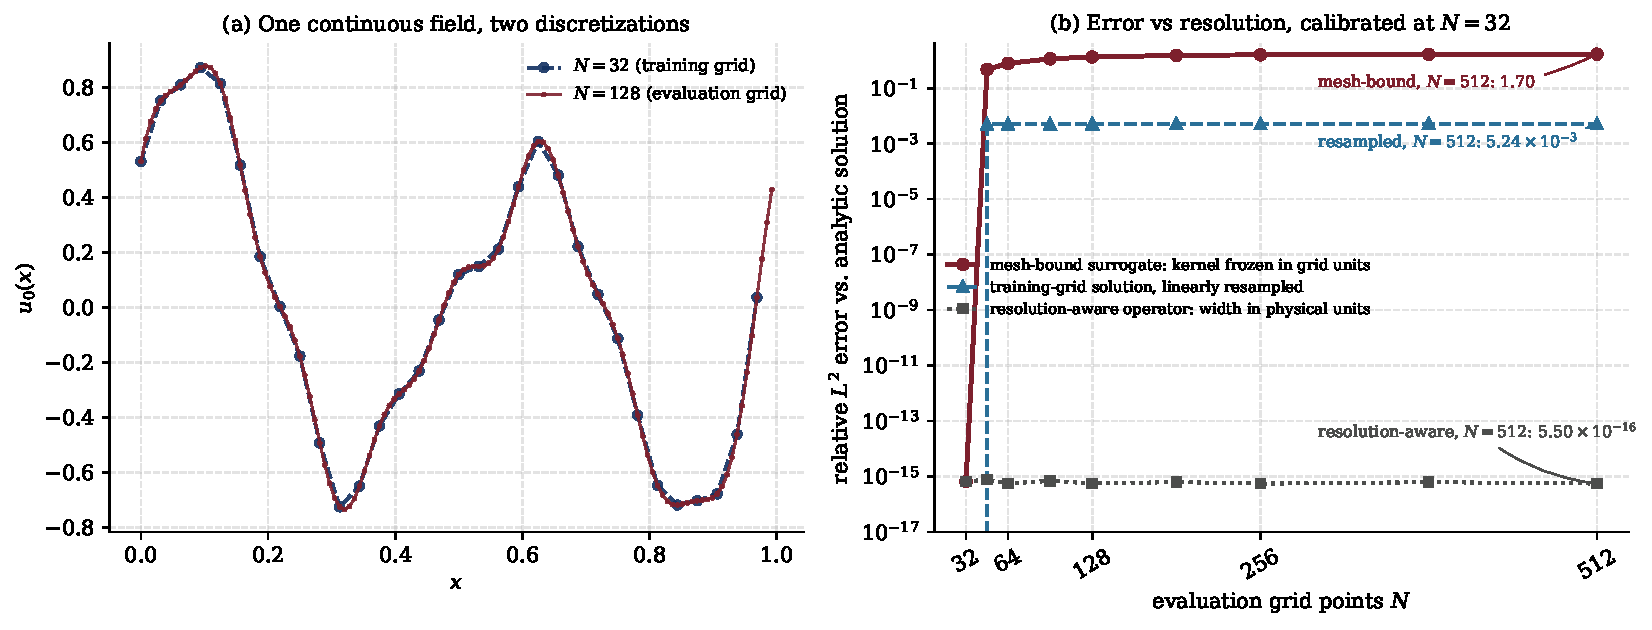
\includegraphics[width=0.92\textwidth]{fig_super_resolution.pdf}
\caption{\textbf{Resolution transfer versus mesh-bound degradation.} (a) The same continuous field from the band-limited input family of Appendix~\ref{app:b}, sampled on a coarse ($N=32$) and a fine ($N=128$) grid of $\mathbb{T}=[0,1)$. (b) Relative $L^2$ error against the analytic heat solution at $T=1$, averaged over 80 inputs, as the \emph{evaluation} grid is refined from $N=32$ to $N=512$ with all operators calibrated at $N=32$. \textbf{No curve, line or marker stands for a trained network:} the one-layer FNO of Appendix~\ref{app:b} is quoted in Section~\ref{sec:appb-result}
and not plotted here, because every curve this plate draws is computed from a solved model;
the trained run's own numbers are quoted in Appendix~\ref{app:b}, whose log and archive are
held with the book. The three curves are computed from discretization error alone and are not trained networks: a mesh-bound smoothing operator whose kernel width is frozen in \emph{grid} units gradually stops smoothing as $N$ grows, reaching $1.70$ at $N=512$; the same operator with its width stated in \emph{physical} units tracks the analytic solution to between $5.48\times10^{-16}$ and
$7.63\times10^{-16}$ on every grid; and solving on the training grid then resampling
linearly plateaus at the interpolation error of the coarse solve, $5.24\times10^{-3}$. \textbf{Caveat, stated once and not to be forgotten:} the test inputs contain only eight Fourier modes and are therefore already fully resolved on the coarse training grid, so the fine-grid evaluation resamples the \emph{same} continuous functions. What the three curves show is what refinement does to a discretization; resolution
transfer of a learned operator is the claim of the quoted experiment of
Appendix~\ref{app:b}, and nothing drawn here establishes it, let alone recovery of
unresolved high-frequency detail. The governing equation is the linear heat equation, whose solution operator is the explicit multiplier $e^{-\alpha(2\pi k)^2 T}$; the network is a teaching example, not evidence that FNOs outperform classical solvers.}
\label{fig:super_resolution}
\end{figure}

Figure~\ref{fig:super_resolution} puts the mechanism and its computed consequences side by
side. Panel (a) shows one continuous field on two discretizations, which is the
operation an invariant model must survive. In panel (b) the mesh-bound curve
degrades exactly as \eqref{eq:ch06-receptive} predicts, the resolution-aware
curve stays at the level of roundoff on every grid, and resampling a
training-grid solution flattens out at the interpolation error of the coarse
solve --- the honest price of the ``interpolate, then run'' workaround. The trained model of Appendix~\ref{app:b} is not in this panel: its reported errors,
$0.0141$ at $N=64$ and the same at $N=256$, are printed by the run re-executed for this book and
archived at \texttt{artifacts/appendix\_b\_run.txt}, and are quoted in
Section~\ref{sec:appb-result} rather than plotted.

What that pair of numbers establishes must be read carefully, and the reading is
less flattering than the usual headline. The inputs carry eight Fourier modes
and are fully resolved on the sixty-four-point grid, so no unresolved detail is
being recovered --- the experiment demonstrates
\emph{resolution transfer}\index{resolution transfer|textbf}, not super-resolution
in the sense of imaging. Moreover the network has a single Fourier layer, so
Proposition~\ref{prop:ch06-zeroshot} applies to its spectral branch with almost
nothing left over. The lift is linear and therefore preserves the band limit;
the twelve retained bins of the real transform cover wavenumbers $0$ through
$11$, so $k_{\max}=11$ sits above the input bandwidth $8$ and far below
$N/2=32$, leaving the Nyquist-type hypothesis of the proposition room to spare;
and the only band-limit-breaking step, the pointwise activation, is not
followed by any further transform. The two discrete norms behind the
identical $0.0141$ are Riemann sums of the same real-analytic error field on
two grids, so their difference is an exponentially small quadrature error, far
below the four decimals that were printed. Both reported numbers are
therefore one number: a model error of order $1.4\%$, printed twice. Both come from one execution, re-run for this book; the archive holds an exemplar
pair rather than the test-set metric, so the printed averages remain the record.
Nothing in the figure shows accuracy at resolutions the data never contained,
and nothing in it shows an advantage over classical solvers for a linear problem
that a single Fourier multiplier solves exactly. That a model \emph{can be
evaluated} on any compatible grid is an architectural property; that it is
\emph{accurate} there is an empirical claim, and it must be re-verified per
problem. The FNO benchmark literature reports models trained on
$64\times64\times20$ space-time data evaluated at $256\times256\times80$
\cite{li2021fourier}, and such reports are observations about the benchmarks
they were run on. The nonlinear, multi-scale problems that motivate operator
learning in the first place are exactly the ones where retained-mode truncation
and sharp moving fronts interact, and where accuracy at a new resolution has to
be demonstrated rather than inferred --- in heterogeneous multiphase flow, the
standard spectral layer resolves fronts less well than an architecture
augmented for fine scales \cite{wen2022ufno}.

\section{Continuum Rates and the Separation of Error Sources}
\label{sec:ch06-rates}

The gap between the exact identity \eqref{eq:ch06-zeroshot} and real multi-layer
networks on rough data is a discretization
error\index{discretization error!algebraic rate} of a particular kind: it sits
between the continuum definition of an FNO and its grid-based realization, with
the parameters held fixed, and is therefore distinct from approximation error
and from estimation error. The estimate this book uses for that gap is the
following.
Write $\Psi_{\text{FNO}}$ for the
continuum network determined by a fixed $\theta$ and $\Psi_{\text{FNO}}^N$ for
its implementation on the $N^d$ grid, and let $v_t$ and $v_t^N$ denote the
corresponding states after $t$ layers. Under the assumptions that the
activations possess bounded continuous derivatives up to order $s$, that the
input set $\mathcal{A}$ is contained in $H^s(\mathbb{T}^d)$ with $s>d/2$, that
the retained modes satisfy $k_{\max}<N/2$, and that the layer parameters are
bounded in the natural norms, the grid error obeys, for every compact
$\mathcal{A}_c \subset \mathcal{A}$,
\begin{equation}
  \label{eq:ch06-rate}
  \sup_{a \in \mathcal{A}_c} \frac{1}{N^{d/2}} \big\| v_t(a) - v_t^N(a) \big\|_{\ell^2(\{x_n\})} \;\le\; C\, N^{-s},
\end{equation}
with $C$ depending on the activation bounds, the parameter bounds, $d$, $s$, the
layer index $t$ and $\mathcal{A}_c$, and the $\ell^2$ norm taken over the $N^d$
nodes of the grid. The same rate holds at the continuum level, with
$\|\Psi_{\text{FNO}}(a)-\Psi_{\text{FNO}}^N(a)\|_{L^2(\mathbb{T}^d)}$ in place of
the grid norm, once the discrete states are replaced by their trigonometric
interpolant. The decay is algebraic, and its
exponent is the Sobolev regularity of the input, inherited by the states it
produces --- the very currency
\chapref{ch:part1-function-spaces-duality-and-sobolev-regula} introduced.

""
elementary, but bounding an entire network requires controlling
$\|v_t\|_{H^s}$ through compositions of nonlinear maps, and that regularity
propagation is where the whole difficulty of \eqref{eq:ch06-rate} sits.
The smoothness requirement is not decorative either, since the exponent is
capped by the least regular object in the pipeline: the rectified linear unit
(ReLU) has regularity only just below $H^{3/2}$ --- its derivative is a step
function --- so with ReLU the decay in \eqref{eq:ch06-rate} saturates once the
input is smoother than that, the ceiling being a property of the activation
rather than of the data, whereas smooth activations such as the Gaussian error
linear unit (GeLU) leave the input regularity to set the rate
\index{ReLU activation!rate saturation}\index{GeLU activation}.
Appending \emph{non-periodic} positional coordinates to a smooth input --- a
standard trick in practical FNO implementations --- introduces a jump across the
boundary of $[0,1]^d$, hence regularity $H^{1/2-\epsilon}$ for every
$\epsilon>0$ and no better, so the exponent available in \eqref{eq:ch06-rate}
falls just short of $1/2$ however smooth the physical channels are.
And the constant grows with the layer index, so the smallness of
\eqref{eq:ch06-rate} is a statement about bounded parameters, not about
well-trained ones. The bound constrains a fixed $\theta$; it says nothing
about whether the $\theta$ obtained by training on grid $N$ coincides with the
one a doubled grid would have produced.

The bookkeeping this suggests is worth writing down once. Let
$\mathcal{E}(n,k_{\max},N)$ denote the error with which a surrogate, trained on
$n$ paired samples stored on the $N$-point grid with $k_{\max}$ retained modes,
reproduces the operator it was trained toward, measured on that same grid. Up
to a multiplicative constant, that error splits as
\begin{equation}
  \label{eq:ch06-decomp}
  \mathcal{E}(n,k_{\max},N)
  \;\lesssim\;
  \underbrace{\mathcal{E}_{\mathrm{stat}}(n)}_{\text{statistical}}
  \;+\;
  \underbrace{\mathcal{E}_{\mathrm{trunc}}(k_{\max})}_{\text{truncation}}
  \;+\;
  \underbrace{\mathcal{E}_{\mathrm{disc}}(N)}_{\text{discretization}},
\end{equation}
a separation made explicit, and rigorous with matching upper and lower bounds for
a discrete-Fourier-transform least-squares estimator of the linear FNO layer, by
Subedi and Tewari \cite{subedi2024controlling}\index{error decomposition!statistical, truncation, and discretization|textbf}.
The truncation term is the spectral truncation of
Theorem~\ref{thm:fno_convergence}, decaying like $k_{\max}^{-\alpha}$ where
$\alpha$ is the smoothing order of that theorem; the discretization term is
\eqref{eq:ch06-rate}; and the statistical term is the generalization error of the
fit, whose sharp form for the operator classes this book learns --- a matching
lower bound, and an estimate whose statistical part does not move with $N$ ---
\chapref{ch:part1-open-theoretical-problems-and-mathematical} lists as open.
Equation \eqref{eq:ch06-decomp} has an immediate practical reading, and it is
the one usually inverted: refining the grid buys nothing once $N^{-s}$ has
dropped below the statistical and truncation floors, while a generous dataset
and a generous $k_{\max}$ can expose a grid error that coarse experiments were
masking. Read in the other direction, the decomposition licenses cheapness ---
if the discretization term dominates early in training, there is no reason to
compute to higher accuracy than the model error --- and that is the logic of
\emph{adaptive subsampling}\index{adaptive subsampling}: train first on a coarse
grid and double the resolution when the validation error plateaus rather than
continuing to improve. Of the three terms of \eqref{eq:ch06-decomp} only
$\mathcal{E}_{\mathrm{disc}}(N)$ responds to refinement, so a loss that stops
falling at fixed $N$ may be resting on the discretization floor rather than on a
model that has stopped learning, and one refinement step is the cheapest
diagnostic that distinguishes the two.

\takeaway{Invariance Is an Architectural Property; Accuracy Is an Empirical One}{%
A neural operator's parameters are indexed by functions rather than by positions
in an array, so one $\theta$ defines a continuum map and a consistent discrete
realization
linked by \eqref{eq:limit_commute}. Exact transfer across grids holds only under
the band-limitedness and Nyquist-type hypothesis $N>2k_{\max}$ of
Proposition~\ref{prop:ch06-zeroshot}; in general the discrete-to-continuum gap
decays algebraically, like $N^{-s}$ with $s$ the Sobolev regularity of the input,
as in
\eqref{eq:ch06-rate}. The reported equality of errors at the $64$- and
$256$-point grids, quoted from Appendix~\ref{app:b} and not plotted in
Figure~\ref{fig:super_resolution}, shows resolution transfer on inputs the coarse grid already
resolved --- not recovery of lost detail, and not superiority over classical
solvers.}

Two questions remain unanswered by \eqref{eq:ch06-decomp}, and both shape the
next chapter. First, the accounting presumes labeled solution data on every grid
it prices: it says how to bill an experiment, not how to learn when labels are
scarce. Second, the errors in \eqref{eq:ch06-rate} and
\eqref{eq:ch06-decomp} are measured in $L^2$-type norms, which constrain the
size of a mistake but not its oscillation --- a surrogate can be accurate in the
mean while its derivatives, and with them its fluxes and its fronts, are wrong.
The remedy in both directions is to put the differential equation into the
objective. The spectral
differentiation that a residual-based loss needs is the same
trigonometric-interpolation machinery that justified \eqref{eq:ch06-zeroshot},
now used to differentiate rather than to resample; and an objective weighted in
$H^1$ or $H^2$ prices exactly the regularity that sets the exponent in
\eqref{eq:ch06-rate}. \chapref{ch:part1-physics-informed-operators-and-sobolev-reg}
develops that move through the physics-informed neural operator
(PINO) \cite{li2021physics} and Sobolev-regularized losses, showing how the
residual term and the mesh-consistent normalization of the objective work
together, and turning the mesh-transfer question raised here into a
training-time constraint.

% Chapter 7: Physics-Informed Operators and Sobolev-Regularized Losses
% Part I of the book.
% STATUS: book-standard prose (Part I).

\chapter{Physics-Informed Operators and Sobolev-Regularized Losses}
\label{ch:part1-physics-informed-operators-and-sobolev-reg}
\label{sec:pino}
% -----------------------------------------------------------------------------

Everything proved so far in this part is an existence statement: an architecture of a given
shape approximates a continuous operator on a compact input set to within $\varepsilon$
(\chapref{ch:part1-operator-approximation-theory-and-universa}), spectral truncation leaves
an error of known order (\chapref{ch:part1-the-fourier-neural-operator-spectral-theor}), and
the discrete realization converges to a mesh-free continuum map
(\chapref{ch:part1-discretization-invariance-and-continuum-li}). None of this names the
parameters a training procedure returns. Between good approximants existing and a minimizer
of a finite-sample least-squares functional being found sits the question this chapter takes
up: what objective should be minimized, and what does it control?
\index{objective functional!in operator learning}

The standard recipe trains against paired solver output: draw inputs, run the simulation,
regress. It fails in three regimes that recur in computation. A three-dimensional
time-resolved solve makes labels scarce. Observational data---fields recorded below the
resolution at which the surrogate will be queried---carry fewer degrees of freedom than the
target function. And when the physics is varied, labels generated for one viscosity or one
forcing family are not labels for the next. In each case the empirical loss has a large flat
set: any candidate reproducing the recorded samples scores identically whether or not it
satisfies the equation elsewhere. Supervision constrains a surrogate where data
exist and leaves it free where they do not.

The remedy developed here is to make the equation part of the objective.
\index{Physics-Informed Neural Network (PINN)}\emph{Physics-Informed Neural Networks}
(PINNs)~\cite{raissi2019physics} minimize a residual for one instance of a
\emph{partial differential equation} (PDE);
\index{Physics-Informed Neural Operator (PINO)}\emph{Physics-Informed Neural Operators}
(PINO)~\cite{li2021physics} impose the same constraint on a whole parametric family, so that
a single trained map is penalized for violating the equation on every input it is shown. Two
further ingredients are then required: derivatives of a network output with respect to
physical coordinates, cheap enough to appear inside every training step; and a choice of the
norm that measures the residual, since a residual is a distribution, not a function, when the
trial field is too rough for the differential expression. Both come from machinery already
assembled: the Sobolev scale and duality pairing of
\chapref{ch:part1-function-spaces-duality-and-sobolev-regula}, the weak formulations of
\chapref{ch:part1-partial-differential-equations-as-solution}, and the multiplier calculus of
\chapref{ch:part1-the-fourier-neural-operator-spectral-theor}.

The chapter proceeds in three moves: the composite loss and what its terms control; how the
residual is differentiated on a grid, and where that computation stops being honest; and what
derivative-based metrics buy. The accounting is explicit throughout: physics enters as a
penalty, penalties cost derivative evaluations, and no choice of weights converts a
regularized least-squares problem into a convergence proof.

% -----------------------------------------------------------------------------
\section{The Variational Loss Functional}
\index{variational loss functional}

Let $\mathcal{N}(\,\cdot\,;a)$\index{$\mathcal{N}$@$\mathcal{N}$, differential expression}
denote a nonlinear differential expression depending on an input field $a$, and let
$\mathcal{B}$\index{$\mathcal{B}$@$\mathcal{B}$, boundary operator} be a boundary or initial
operator. The parametric problems collected in
\chapref{ch:part1-partial-differential-equations-as-solution} all fit the form
\begin{equation}
  \label{eq:ch07-bvp}
  \begin{cases}
    \mathcal{N}(u; a) = 0, & x \in \Omega, \\
    \mathcal{B}(u; a) = 0, & x \in \partial\Omega.
  \end{cases}
\end{equation}
For a stationary problem $\mathcal{N}$ is the elliptic expression $-\nabla\cdot(a\nabla u)-f$
of Darcy flow; for an evolutionary one the unknown $u$ is read as a trajectory in the
Bochner space $L^2(0,T;\mathcal{U})$ introduced in
\chapref{ch:part1-function-spaces-duality-and-sobolev-regula} and $\mathcal{N}$ contains
$\partial_t$. The exact solution map is $\mathcal{G}_{\text{true}}:a\mapsto u$, the surrogate
is $\mathcal{G}_\theta$. Inputs are drawn from a probability measure
\index{$\mu$@$\mu\in\mathcal{P}(\mathcal{A})$, training measure}$\mu\in\mathcal{P}(\mathcal{A})$, the same measure whose
support supplies the compact sets of the universality
theorems. All expectations below are population quantities; stochastic training replaces
each by a minibatch average, which is the only place where discretization enters the
objective.

The composite training loss for a parameter vector $\theta$ is
\begin{equation}
  \label{eq:pino_loss}
  \mathcal{L}_{\text{PINO}}(\theta) = \lambda_{\text{data}} \mathcal{L}_{\text{data}}(\theta) + \lambda_{\text{pde}} \mathcal{L}_{\text{pde}}(\theta) + \lambda_{\text{bc}} \mathcal{L}_{\text{bc}}(\theta),
\end{equation}
\index{PDE residual penalty}\index{loss weighting!$\lambda$ coefficients}where
\begin{align}
  \mathcal{L}_{\text{data}}(\theta) &= \mathbb{E}_{a \sim \mu} \left[ \frac{\|\mathcal{G}_\theta(a) - \mathcal{G}_{\text{true}}(a)\|_{L^2(\Omega)}^2}{\|\mathcal{G}_{\text{true}}(a)\|_{L^2(\Omega)}^2} \right], \label{eq:ch07-data-loss}\\
  \mathcal{L}_{\text{pde}}(\theta) &= \mathbb{E}_{a \sim \mu} \left[ \|\mathcal{N}(\mathcal{G}_\theta(a); a)\|_{X(\Omega)}^2 \right], \label{eq:ch07-pde-loss}\\
  \mathcal{L}_{\text{bc}}(\theta) &= \mathbb{E}_{a \sim \mu} \left[ \|\mathcal{B}(\mathcal{G}_\theta(a); a)\|_{Y(\partial\Omega)}^2 \right]. \label{eq:ch07-bc-loss}
\end{align}
Set $\lambda_{\text{pde}}=\lambda_{\text{bc}}=0$ in \eqref{eq:pino_loss} and only
\eqref{eq:ch07-data-loss} survives: that is supervised regression on paired simulations, the
procedure the previous chapters analyzed. The two added terms
\eqref{eq:ch07-pde-loss}--\eqref{eq:ch07-bc-loss} measure, respectively, how much the
predicted field violates the equation inside $\Omega$ and how much it violates the imposed
trace on $\partial\Omega$.

Two features of \eqref{eq:ch07-data-loss}--\eqref{eq:ch07-bc-loss} repay attention. Only the
data term is normalized by the energy of its target, so it is scale-free and dimensionless;
the residual and boundary terms carry the physical units of $\mathcal{N}$ and
$\mathcal{B}$. Consequently $\lambda_{\text{pde}}$ and $\lambda_{\text{bc}}$ are dimensional
quantities whose usable size depends on the nondimensionalization chosen for the problem,
and balancing the three terms is a hyperparameter decision rather than a consequence of the
formulation. Next, the terms are not independent constraints but penalties: what
physics-informed training really asserts is a conditional. If a parameter $\theta^{*}$
annihilates all three terms, then $\mathcal{G}_{\theta^{*}}(a)=\mathcal{G}_{\text{true}}(a)$
for $\mu$-almost every $a$, \emph{provided} the problem \eqref{eq:ch07-bvp} has a unique
solution in the class containing both fields. Well-posedness---the Lax--Milgram argument of
\chapref{ch:part1-partial-differential-equations-as-solution}---is therefore a hypothesis of
the method, not background decoration. What the residual term changes about data
requirements is visible in this statement: instead of requiring a full solution field as a
label, an input $a$ together with the equation supplies a target, and the two can be
combined at different resolutions, as in the coarse-data, fine-residual training reported
in~\cite{li2021physics}.

The choice of the space $X(\Omega)$ in \eqref{eq:ch07-pde-loss} is where the functional
analysis does work. With $X=L^2(\Omega)$ the residual is evaluated in the \emph{strong form},
pointwise on the grid, which demands that the trial field possess as many classical
derivatives as $\mathcal{N}$ has. With $X=H^{-s}(\Omega)$, $s>0$, the residual is measured in
the \emph{weak form}: for a trial field $v=\mathcal{G}_\theta(a)$ whose residual is denoted
$r_v$, the norm is the dual one,
$\|r_v\|_{H^{-s}}=\sup_{\varphi\neq0}|\langle r_v,\varphi\rangle|/\|\varphi\|_{H^{s}}$, and
integration by parts transfers derivatives from $v$ onto the smooth test function
$\varphi$. For a second-order divergence-form operator the
strong residual needs two derivatives of $v$ while the weak residual needs one. By Parseval's
identity the same distinction is a weighting of modal coefficients,
$\|r_v\|_{H^{-s}}^{2}=\sum_{k}(1+|k|^{2})^{-s}|\hat{r}_v(k)|^{2}$---a relaxation of
attention on fine scales, in direct contrast with the sharpening that the Sobolev-norm
penalty of the third section performs.

For coercive problems the weak penalty is more than a convention: it controls the error. Take
the Darcy problem under uniform ellipticity, with $v\in H^1_0(\Omega)$ a trial field of the
correct trace and $r_v$ its weak residual,
$\langle r_v,w\rangle:=\int_\Omega a\nabla v\cdot\nabla w\,dx-\langle f,w\rangle_{H^{-1},H^1_0}$.
Subtracting the weak form of the exact solution from that of $v$, testing with
$w=v-\mathcal{G}_{\text{true}}(a)$, and using coercivity
$B_a(e,e)\ge a_{\min}\|\nabla e\|_{L^2}^2$ gives the a priori estimate
\begin{equation}
  \label{eq:ch07-apriori}
  \big\|\nabla(v-\mathcal{G}_{\text{true}}(a))\big\|_{L^2(\Omega)}
  \;\le\; \frac{1}{a_{\min}}\,\|r_v\|_{H^{-1}(\Omega)}.
\end{equation}
Here $\|\cdot\|_{H^{-1}(\Omega)}$ is the dual of the energy norm
$\|\nabla\cdot\|_{L^2(\Omega)}$ on $H^1_0(\Omega)$; measured against the full $H^1$ norm, a
Poincar{\'e} constant joins the right-hand side, as in
\chapref{ch:part1-partial-differential-equations-as-solution}. This is the precise sense in
which minimizing \eqref{eq:ch07-pde-loss} substitutes for
labeling: the estimate \eqref{eq:ch07-apriori} says that a small weak residual plus a correct
trace forces a small energy-norm error. Read it
also as a warning, because the estimate is conditional on coercivity and degrades as
$a_{\min}\to0$; where no such estimate is available---the inviscid limit, formation of
shocks---a small residual is not evidence of a small error. It is worth recording that the
empirical ranking does not follow the analysis: in the Darcy experiments reported in~\cite{li2021physics},
the strong-form residual trained better than the weak-form one, which
suggests that the test space is an implementation choice entangled with how derivatives are
computed, taken up next.

The boundary term deserves one further comment. On the torus $\mathbb{T}^d$ there is no
$\partial\Omega$, so \eqref{eq:ch07-bc-loss} vanishes identically and the vorticity-form
Navier--Stokes problem of \chapref{ch:part1-partial-differential-equations-as-solution} is
trained on data and residual alone. Where a boundary does exist, \eqref{eq:ch07-bc-loss} is
still a soft penalty. The alternative is a hard constraint---compose the surrogate with a
lifting of the boundary data so that the trace is satisfied by construction---which removes
one weight from the hyperparameter list but requires the trace operator to be meaningful for
the output regularity at hand, that is $v\in H^{s}(\Omega)$ with $s>1/2$.

% -----------------------------------------------------------------------------
\section{Spectral Differentiation in Operator Learning}
\index{spectral differentiation}\index{pseudo-spectral method}

In a PINN~\cite{raissi2019physics} the network is itself the solution ansatz,
$u_\theta:x\mapsto u(x)$, evaluated at scattered collocation points, and the spatial
derivatives $\partial_x u$ and $\partial_{xx}u$ in the residual are obtained by reverse-mode
automatic differentiation. Nothing is approximated there in the numerical-analysis sense:
the derivative is exact for the model, since the model is a differentiable function of $x$.
The price is structural. A second derivative requires a second backward pass through the
computational graph, time and memory grow with depth times the number of collocation points,
and each point is evaluated independently, so representing a field means representing its
samples.

A neural operator is organized the other way round. Its output is a field on a discretization
$\mathcal{M}_N$, and its internal spectral layer---a learned Fourier multiplier, as
\chapref{ch:part1-the-fourier-neural-operator-spectral-theor} constructs it---is a global
operation on that field, defined only for the whole grid at once. Querying such a network at
a single coordinate $x$ means running the transforms; forcing it into a form on which
automatic differentiation yields second $x$-derivatives is possible but forfeits exactly the
structure that made the architecture cheap. When the output is a discrete field on a periodic
mesh $\mathbb{T}^d$, spatial derivatives can instead be evaluated directly in Fourier space:
\begin{equation}
  \label{eq:spectral_diff}
  \frac{\partial^m \mathcal{G}_\theta(a)}{\partial x_j^m} = \mathcal{F}^{-1} \left( (2\pi i k_j)^m \cdot \mathcal{F}\big( \mathcal{G}_\theta(a) \big)(k) \right).
\end{equation}
The identity is one line. For $N$ equispaced nodes of $[0,1)^d$ with discrete Fourier
coefficients $\hat v(k)$ of a grid function $v$, differentiation of the trigonometric
interpolant acts diagonally,
\begin{equation}
  \label{eq:ch07-diff-prop}
  \big(\mathcal{F}(\partial_{x_j}^{m} v)\big)(k) = (2\pi i k_j)^{m}\,\hat v(k),
  \qquad k\in\mathbb{Z}^{d},
\end{equation}
and \eqref{eq:spectral_diff} is \eqref{eq:ch07-diff-prop} followed by the inverse transform.
\index{Fourier multiplier!differentiation as}

Two consequences make this the right tool for a physics-informed operator. First,
\eqref{eq:ch07-diff-prop} is a Fourier multiplier with symbol $(2\pi i k_j)^m$: the very
primitive the architecture already applies, with the learned tensor $R_\phi(k)$ replaced by a
fixed one. Differentiating a field costs two traversals of the
\emph{fast Fourier transform} (FFT) pipeline, $\mathcal{O}(N\log N)$ operations for the
entire field at once, rather than a per-point differentiation of a network graph. Second,
\eqref{eq:spectral_diff} is exact on band-limited inputs and, for smooth ones, converges
faster than any power of the mesh width: if $v$ extends analytically to a complex
neighborhood of the torus, its coefficients decay geometrically, so truncating at $k_{\max}$
leaves an error in the $m$-th derivative of the same exponential order, whereas a finite
difference of order $p$ carries a truncation error $\mathcal{O}(h^{p})$ that shrinks only
algebraically~\cite{leveque2002finite}. \index{exponential convergence!of spectral differentiation}

Both statements need qualifying, and the qualification matters more than the advantage. What
\eqref{eq:spectral_diff} differentiates is the interpolant of the stored samples, not the
continuum field they came from. Where the two differ, the discrepancy is amplified rather
than damped, because the symbol in \eqref{eq:ch07-diff-prop} has magnitude
$(2\pi|k|)^{m}$: an error component at the highest resolvable wavenumber $k\approx N/2$ is
multiplied by $(\pi N)^{m}$ in the $m$-th derivative, so grid-scale noise or truncation
content dominates a residual built this way. For even $N$ the Nyquist coefficient is not
resolved by the samples at all---two interpolants agree at the nodes and disagree in their
derivative---and it is conventionally discarded before an odd-order
differentiation~\index{aliasing!in spectral derivatives}\index{Nyquist mode}. Nor is a
nonlinear residual free of the same difficulty.
\begin{example}[pseudo-spectral Burgers residual]
For $\mathcal{N}(u) = \partial_t u + u\,\partial_x u - \nu\,\partial_{xx}u$ on $\mathbb{T}$,
each linear term comes from \eqref{eq:spectral_diff}, while the product $u\,\partial_x u$ is
formed pointwise on the grid and, if it is ever transformed again, contains wavenumbers
beyond the cutoff that fold back onto resolved modes. Classical dealiasing (zero-padding or
the two-thirds rule) suppresses that \emph{aliasing}; a PINO implementation inherits the
requirement because the residual is recomputed every step. The same restriction is recorded
in~\cite{li2021physics}: spectral differentiation presumes smoothness and a uniform grid, and
derivative error is amplified downstream in the predicted solution. For fields with jumps,
such as the vanishing-viscosity Burgers limit discussed in
\chapref{ch:part1-partial-differential-equations-as-solution}, no nodal differentiation rule
is accurate---the Gibbs phenomenon identified as an open problem in
\chapref{ch:part1-open-theoretical-problems-and-mathematical} is precisely this failure.
\end{example}

Finally, note where the differentiation is \emph{not} taken. In
\eqref{eq:spectral_diff} the derivatives are with respect to the physical coordinates $x$, at
fixed $\theta$; the training gradient still requires derivatives with respect to $\theta$,
computed by backpropagation through the field-producing network. Because the operator in
\eqref{eq:ch07-diff-prop} is linear, its adjoint is the multiplier with the conjugated
symbol, so the backward pass through a spectral derivative is another pair of FFTs rather
than a second-order differentiation of the network graph. The practical cost is therefore
memory, not algebra: intermediates of the forward pass must be retained so that the residual
branch can be differentiated, and the residual must be assembled at every grid point of every
sample in every step.

% -----------------------------------------------------------------------------
\section{Sobolev \texorpdfstring{$H^1$ and $H^2$}{H1 and H2} Norm Regularization}
\index{Sobolev space!$H^1$ regularization}\index{Sobolev space!$H^2$ regularization}

Training neural operators solely with the relative $L^2$ loss \eqref{eq:ch07-data-loss} can
lead to \emph{spectral bias}\index{spectral bias}, where the model captures low-frequency
energy but exhibits phase errors or high-frequency oscillations in gradients. The mechanism
is visible in Fourier coefficients. Write the prediction error as
$e_\theta(a)=\mathcal{G}_\theta(a)-u$, where $u=\mathcal{G}_{\text{true}}(a)$ is the label
field. Parseval's identity gives
$\|e_\theta\|_{L^2}^{2}=\sum_k|\hat e_\theta(k)|^{2}$ while
$\|\partial_{x_j}e_\theta\|_{L^2}^{2}=\sum_k(2\pi k_j)^2|\hat e_\theta(k)|^{2}$, so a defect
at wavenumber $k$ counts $(2\pi|k|)^2$ times more heavily in the derivative metric than in
the $L^2$ metric. Since the target's own spectrum decays with $|k|$
(cf.\ the coefficient bound in \chapref{ch:part1-the-fourier-neural-operator-spectral-theor}),
residual error is concentrated exactly where relative $L^2$ error is nearly blind, and a
first-order optimizer spends its early iterations on the high-energy modes.

Regularizing the objective with higher Sobolev norms enforces derivative fidelity:
\begin{equation}
  \label{eq:ch07-sobolev-loss}
  \mathcal{L}_{H^s}(\theta) = \mathbb{E}_{a \sim \mu} \left[ \frac{\|\mathcal{G}_\theta(a) - u\|_{L^2}^2}{\|u\|_{L^2}^2} + \beta \sum_{j=1}^d \frac{\|\partial_{x_j} \mathcal{G}_\theta(a) - \partial_{x_j} u\|_{L^2}^2}{\|\partial_{x_j} u\|_{L^2}^2} \right].
\end{equation}
The sum runs over the $d$ coordinate
directions, and $\beta$\index{$\beta$@$\beta$, derivative-tradeoff weight} balances the two
quotients. In spite of the subscript, \eqref{eq:ch07-sobolev-loss} controls values and first
derivatives only, that is the inhomogeneous $H^1$ norm; the $H^2$ case named in the section
title appends the second multi-index terms, which in Fourier variables means weighting modal
errors by $(1+|k|^{2})^{2}$ rather than $(1+|k|^{2})^{1}$. Read this way, \eqref{eq:ch07-sobolev-loss}
and the negative-norm residual penalty of \eqref{eq:ch07-pde-loss} are the same device on
opposite sides of the Sobolev scale\index{Sobolev space!as objective weighting}: a positive
index sharpens attention on fine structure, a negative index relaxes it.

\index{Sobolev embedding theorem!and $L^\infty$ control}What the sharpening buys is a change
of metric, and one metric inequality. The Sobolev embedding theorem
(\chapref{ch:part1-function-spaces-duality-and-sobolev-regula}; see
also~\cite{evans2010partial,brezis2011functional}) states that $H^{s}(\Omega)\hookrightarrow
C^{k}(\overline{\Omega})$ continuously when $s>d/2+k$, so with $k=0$ an error $e$ obeys
$\|e\|_{L^\infty}\le C_s\|e\|_{H^{s}}$. Controlling $\|\cdot\|_{H^s}$ with $s>d/2$ therefore
excludes localized pointwise spikes: no defect can be large somewhere without being large in
the norm the objective measures. The statement is an implication between metrics, not an
algorithmic guarantee---nothing in \eqref{eq:ch07-sobolev-loss} forces the optimizer to make
that norm small, and in dimension $d=3$ the hypothesis $s>d/2$ requires two derivatives,
which is why the $H^2$ variant rather than the $H^1$ one is the natural target for
three-dimensional fields. It is also why such losses are attractive independently of any
physics term: the quantities practitioners read off a simulation are derivatives of the
state---the Darcy flux $-a\nabla u$, the vorticity $\nabla\times u$, the wall shear
stress---so an $L^2$-accurate field may still be a poor model of the diagnostic. The
companion claim, that derivative regularization preserves conservation properties, should be
read in the same register: it suppresses non-physical oscillation in gradients, which is
consistent with better behaved balance laws, but it is not a proof that a trained network
satisfies any conservation identity.

\index{discretization invariance!of the loss functional}A second consistency check comes from
\chapref{ch:part1-discretization-invariance-and-continuum-li}. Each quotient in
\eqref{eq:ch07-sobolev-loss} approximates a ratio of integrals, so on $N$ nodes the sums must
carry the cell volume $h^{d}$ to be quadratures at all; the relative normalization then cancels
the remaining mesh factor, which is why the objective is a mesh-consistent quantity whereas an
unnormalized discrete seminorm grows with refinement. The normalization has its own failure
mode: when $\|\partial_{x_j}u\|_{L^2}$ is small---a label that is nearly constant along a
coordinate, as for shear-driven or symmetry-reduced data---the corresponding term is
ill-conditioned and its gradient is dominated by the surrogate's own derivative fluctuation.
Normalizing over a batch instead of per sample repairs the scaling but makes an individual
sample's contribution depend on which other samples were drawn.

\index{no free lunch!in physics-informed regularization}It remains to state what the two
regularization devices cost, since neither is free. A Sobolev-metric loss requires
differentiating the label as well as the prediction; for fixed grid-function labels those
derivatives can be computed once offline, but the prediction derivatives recur at every
step. A physics-informed loss requires assembling \eqref{eq:ch07-bvp} on the surrogate's
output at every step, adding spectral derivatives, nonlinear pointwise products, and a
backward pass through them, and adding two further hyperparameters to
\eqref{eq:pino_loss}. Neither penalty alters the approximation classes of
\chapref{ch:part1-operator-approximation-theory-and-universa}: they change which element of
the class is found, not which elements exist. Nor do they immunize training against the
equation being wrong---when $\mathcal{N}$ encodes a closure or a solver's discretization
rather than the physics of interest, the residual term biases the fit away from the data that
was generated by that same model. The reported benefits are correspondingly empirical and
specific: PINO trained with both terms is reported to need fewer labels than a purely
data-driven \emph{Fourier Neural Operator} (FNO), to generalize better at resolutions
above the training one, and on transient
and Kolmogorov flows to reduce average relative error by roughly $7\%$, while remaining
trainable in a data-free regime where a PINN is reported to fail on the optimization
landscape of the PDE constraint~\cite{li2021physics,raissi2019physics}. Those are benchmark
outcomes, not theorems, and they are the honest boundary of what this chapter can claim.

% -----------------------------------------------------------------------------

What this chapter leaves unresolved is comparative. It treated the objective as if it were
architecture-independent, and \eqref{eq:pino_loss} is not: the residual term is cheap when
\eqref{eq:spectral_diff} applies, which requires a uniform periodic grid and a field smooth
enough that the multiplier's $(2\pi|k|)^m$ amplification is harmless; it must be rebuilt from
graph or mesh-based difference operators on the unstructured discretizations that the
geometry-informed architectures use; and for an architecture whose input is a fixed sensor
vector, the data term and the residual term are not measured on comparable discretizations at
all. Likewise the derivative penalties of \eqref{eq:ch07-sobolev-loss} presuppose that
$\partial_{x_j}\mathcal{G}_\theta(a)$ has a well-defined discrete meaning. \chapref{ch:part1-comparative-theoretical-taxonomy-of-archit}
assembles these axes into a single comparison---input format, coordinate query, kernel
parameterization, cost per layer, discretization invariance, and support for physics-residual
evaluation---across DeepONet, the generic neural operator, the FNO, and the geometry-informed
neural operator. Reading it after this chapter is worthwhile precisely because the two
decisions it tabulates, how to represent a map and what to minimize, are one decision made
twice.

% Chapter 8: Comparative Theoretical Taxonomy of Architectures
% Part I of the book.

\chapter{Comparative Theoretical Taxonomy of Architectures}
\label{ch:part1-comparative-theoretical-taxonomy-of-archit}
\label{sec:taxonomy}
\index{operator architectures!taxonomy of|textbf}
\index{taxonomy!of operator architectures|textbf}
% -----------------------------------------------------------------------------

The seven chapters that precede this one developed the theory in a single direction: function spaces and their compact embeddings in \chapref{ch:part1-function-spaces-duality-and-sobolev-regula}, PDE (partial differential equation) solution operators and their regularity in \chapref{ch:part1-partial-differential-equations-as-solution}, approximation theorems in \chapref{ch:part1-operator-approximation-theory-and-universa}, the spectral construction that makes one of those theorems cheap in \chapref{ch:part1-the-fourier-neural-operator-spectral-theor}, mesh independence in \chapref{ch:part1-discretization-invariance-and-continuum-li}, and training functionals in \chapref{ch:part1-physics-informed-operators-and-sobolev-reg}. Read in that order, the architectures look like answers to different questions. DeepONet (Deep Operator Network) \index{DeepONet|(} asks how many point samples pin down a function; the generic neural operator (NO) \index{generic neural operator|(} asks whether trainable integral kernels are dense in the continuous operators; the FNO (Fourier Neural Operator) asks what an integral kernel costs once it is translation invariant; the geometry-informed variant asks what changes when the domain is a car body rather than a torus; and a last question, what changes when the array of learned multipliers is too large to store, is treated here purely as a factorization technique rather than as an architecture.

Put side by side, those questions generate one no single paper settles: which architecture suits which class of problems, and on what grounds? The question is hard for three reasons. First, the architectures are not rivals contesting a common task; each restricts the same integral-kernel template of \eqref{eq:no_layer} to a smaller function class, so a fair comparison must say what every restriction forfeits and what it purchases. Second, the axes are chosen rather than given: expressiveness, inductive bias, dependence on the discretization, cost per query, and the strength of available convergence guarantees are logically independent, and an architecture can be first on one and last on another. Third, the evidence is uneven in kind. Some entries rest on proved theorems, some on arithmetic over a fixed discretization, some only on published experiments; blending those registers into one table is how a taxonomy turns misleading.

This chapter fixes the axes, states what each architecture assumes, and keeps an explicit ledger of what is proved and what is not. Section~\ref{sec:ch8-axes} defines the axes and writes out the two inclusions that make the architectures comparable at all. Section~\ref{sec:ch8-requirements} asks what each requires of the target operator and records the theorems attached to each requirement. Section~\ref{sec:ch8-cost} does the cost accounting, assembles Table~\ref{tab:comparison} and the theorem ledger Table~\ref{tab:ch8-ledger}, and marks the limits of the comparison. Prerequisites are Chapters~\ref{ch:part1-operator-approximation-theory-and-universa}--\ref{ch:part1-physics-informed-operators-and-sobolev-reg}, plus the function-space and solution-operator material of \chapref{ch:part1-function-spaces-duality-and-sobolev-regula} and \chapref{ch:part1-partial-differential-equations-as-solution} behind them; no new result is proved here. What the chapter leaves blank is the subject of \chapref{ch:part1-open-theoretical-problems-and-mathematical}.

% -----------------------------------------------------------------------------
\section{Axes of Comparison}
\label{sec:ch8-axes}
% -----------------------------------------------------------------------------

Comparison requires a common template, and the template is the one introduced in \chapref{ch:part1-operator-approximation-theory-and-universa}: a lift $\mathcal{P}$, a stack of layers \eqref{eq:no_layer} carrying a local linear map $W_\ell$, a bias $b_\ell$, an activation $\sigma$ and a non-local integral operator $\mathcal{K}_\ell$ with kernel $\kappa_\ell(x,y,a(x),a(y);\phi_\ell)$ as in \eqref{eq:fredholm_kernel}, and a projection $\mathcal{Q}$. Every architecture keeps that skeleton and constrains $\kappa_\ell$ differently. \index{kernel!constraints across architectures}

The first axis is the size of the kernel class: how large a set of operators the parameterization spans as the free parameters $\phi_\ell$ range over all admissible values. The generic neural operator imposes nothing beyond continuity of $\kappa_\ell$ on $\Omega\times\Omega$ and dependence on the input values at the pair $(x,y)$ \cite{kovachki2023neural}. The FNO is the same layer with two restrictions at once --- the domain becomes the torus $\mathbb{T}^d$, and the kernel becomes stationary and input-independent,
\begin{equation}
  \label{eq:ch8-fno-specialization}
  \kappa_\ell(x,y,a(x),a(y);\phi_\ell) \;=\; \kappa_\ell(x-y;\phi_\ell),
  \qquad
  R_\phi(k) \;=\; \int_{\mathbb{T}^d} \kappa_\ell(z;\phi_\ell)\, e^{-2\pi \mathrm{i} k\cdot z}\, \mathrm{d}z,
\end{equation}
\index{Fourier multiplier $R_\phi(k)$}\index{kernel!translation-invariant (stationary)}
so the integral of \eqref{eq:fredholm_kernel} becomes multiplication by the Fourier multiplier $R_\phi(k)$, which is exactly the convolution theorem invoked to reach \eqref{eq:fno_layer}. DeepONet sits at the opposite corner: its hypothesis class is not described by a kernel over $\Omega\times\Omega$ at all, but by $m$ point evaluations of the input and a rank-$p$ decomposition of the output in the query coordinates $y$ \cite{lu2021learning}. Written in kernel language, the two halves of that statement read
\begin{equation}
  \label{eq:ch8-deeponet-kernel}
  \big(\mathcal{K}v\big)(x) \;=\; \sum_{j=1}^{m} \kappa(x,x_j)\, v(x_j)\, w_j,
  \qquad
  \kappa(x,y) \;=\; \sum_{r=1}^{p} t_r(x)\, \xi_r(y),
\end{equation}
the left identity being the branch side --- integration against a measure carried by $m$ prescribed sensors $x_j$ with weights $w_j$, rather than against $\mathrm{d}y$ over the whole domain --- and the right identity being the trunk side, a kernel of rank $p$ in the pair $(x,y)$: $t_r$ are the trunk functions of the output point, the basis constructed in \chapref{ch:part1-operator-approximation-theory-and-universa}, while $\xi_r$ is a function of the input coordinate that a trained branch replaces by a sensor-weighted combination. Graph-based operators constrain the \emph{support} of the kernel instead of its algebraic form: a Graph Neural Operator (GNO) \index{Graph Neural Operator (GNO)|(} layer integrates over the ball $\mathcal{B}_r(x_i)$ about each node, with an input-dependent kernel of the generic shape evaluated on relative coordinates and a quadrature weight $w_j$ given by the Voronoi dual measure of the vertex \cite{li2023geometry,brandstetter2022message}. The Geometry-Informed Neural Operator (GINO) \index{Geometry-Informed Neural Operator (GINO)|(} composes such layers with an FNO acting on a regular latent grid \cite{li2023geometry}. A restriction of a different kind acts on the multiplier array rather than on the kernel it represents: the array $R_\phi(k)$ is reshaped into three indices and constrained to low multilinear \emph{rank}. That last item is a factorization technique, not an entry in the comparison, and its arithmetic is done in Section~\ref{sec:ch8-cost}.

Inductive bias, the second axis, is the one most often left vague, so it repays stating negatively: what the parameterization cannot do. A multiplier as in \eqref{eq:ch8-fno-specialization} acts diagonally across modes, so one spectral layer may rotate the channel vector within the mode $k$ but never moves energy between distinct $k$; transfer of energy between modes comes from the activation $\sigma$ and the pointwise bypass $W_\ell$, which mix frequencies in physical space, not from the kernel. A trunk of rank $p$, as in the right identity of \eqref{eq:ch8-deeponet-kernel}, confines its outputs to a $p$-dimensional subspace however the branch is trained. A radius-$r$ graph kernel transmits nothing farther than $r$ in one layer, which is why GINO pairs its graph encoder with a global spectral operator rather than merely deepening the graph. Each negative statement has a price tag, collected in Section~\ref{sec:ch8-cost}.

The third axis is the relation between parameter space and discretization: whether the parameters are mesh-free in the sense of the diagram around \eqref{eq:limit_commute}, and whether what the code evaluates is the continuum operator or one of its discretizations. The fourth is cost per query, the fifth the strength of the rigorous statement available for the class --- universality without a rate, a rate under hypotheses, a complexity count, or nothing at all. Section~\ref{sec:ch8-cost} supplies the arithmetic and Section~\ref{sec:ch8-requirements} the hypotheses, so that each cell of Tables~\ref{tab:comparison} and~\ref{tab:ch8-ledger} can be checked rather than trusted.

\begin{remark}[The inclusions above are formal, not literal]
\label{rmk:ch8-inclusions}
Neither identification is an equality of operators on function spaces of the kind stated in \eqref{eq:no_composition}. In \eqref{eq:ch8-deeponet-kernel} the sensor sum represents integration against the discrete measure $\sum_j w_j\delta_{x_j}$, and a Dirac mass $\delta_{x_j}$ belongs to $H^{-s}(\Omega)$ for $s>d/2$ but not to $L^2(\Omega)$; the expression is meaningful only once the input space is regular enough for point evaluation to be a bounded functional, which is the Sobolev embedding condition of \chapref{ch:part1-function-spaces-duality-and-sobolev-regula}. \index{point evaluation}\index{Dirac measure!as sensor model} Likewise, \eqref{eq:ch8-fno-specialization} discards the $a(x),a(y)$ arguments of the generic kernel, which restricts the \emph{layer} and makes no physical claim about the target operator. Reading these identities as nesting relations between hypothesis classes is safe; reading them as assertions that one architecture is a special case of another on a shared function-space domain is not.
\end{remark}

% -----------------------------------------------------------------------------
\section{What Each Architecture Requires of the Target Operator}
\label{sec:ch8-requirements}
% -----------------------------------------------------------------------------

The requirements differ more than the guarantees do, and they are where most misuse of the comparison begins.

For the generic neural operator the requirement is the one in Theorem~\ref{thm:no_universality}: $\mathcal{G}$ must be continuous on a compact set $K\subset L^2(\Omega;\mathbb{R}^{d_a})$ with values in $L^2(\Omega;\mathbb{R}^{d_u})$ \cite{kovachki2023neural}. Compactness is not cosmetic. Part~I obtained it from smoothing: a solution operator mapping bounded sets into a higher Sobolev space, $\mathcal{G}:H^s\to H^{s+\alpha}$ with $\alpha>0$, has precompact image by Rellich--Kondrachov, which is why the elliptic and parabolic problems of \chapref{ch:part1-partial-differential-equations-as-solution} fall inside the theorem's reach on the strength of the compact embedding of \chapref{ch:part1-function-spaces-duality-and-sobolev-regula}, while a pure transport map that translates a discontinuity without regularizing it does not. \index{smoothing order $\alpha$} What the theorem does not supply is a rate. It asserts the existence of depth $L$, width $d_v$ and continuous kernels $\kappa_\ell$ with $\sup_{a\in K}\|\mathcal{G}(a)-\mathcal{G}_\theta(a)\|_{L^2}<\varepsilon$, and is silent on how large $L$, $d_v$ or the kernel parameters must become as $\varepsilon\to0$. Discretization invariance is a separate property, established for this class through the quadrature-consistency argument behind \eqref{eq:limit_commute} rather than as a corollary of universality.

DeepONet inherits the same qualitative hypothesis --- continuity on compacta, from Theorem~\ref{thm:chen_chen} \cite{chen1995universal} --- and adds two requirements of its own, one on inputs, one on outputs. Inputs must be recoverable from $m$ point samples, which presupposes the regularity noted in Remark~\ref{rmk:ch8-inclusions}; outputs must be approximable by a $p$-dimensional subspace, since the trunk functions of \eqref{eq:ch8-deeponet-kernel} span at most $p$ directions. The reward for accepting both is that Theorem~\ref{thm:no_universality}'s silence on rates is partly broken: the three-term decomposition proved for DeepONet in \chapref{ch:part1-operator-approximation-theory-and-universa} \cite{lanthaler2022error} separates sensor, basis and network contributions, and each can be attacked on its own terms. For inputs in the unit ball of $H^s(\Omega)$, inverting the compact-embedding scaling $\log\mathcal{N}(\varepsilon,B_{H^s},L^2)\sim\varepsilon^{-d/s}$, recalled in \chapref{ch:part1-open-theoretical-problems-and-mathematical}, gives the sensor term the decay
\begin{equation}
  \label{eq:ch8-sensor-rate}
  \mathcal{E}_{\mathrm{sensor}}(m) \;\lesssim\; m^{-s/d},
  \qquad s > d/2,
\end{equation}
\index{sampling error!rate $m^{-s/d}$}\index{covering number}
where the exponent measures how fast information is lost as the sampling set stays fixed and the field becomes rougher. Equation \eqref{eq:ch8-sensor-rate} is recorded as the expectation those covering asymptotics justify, not as a bound for a trained network: a sharp non-asymptotic sample-complexity statement for nonlinear operators is open, as \chapref{ch:part1-open-theoretical-problems-and-mathematical} makes explicit.

The FNO demands the most. It requires a periodic or toroidal domain, fields represented on a grid that the discrete Fourier transform acts on, and, for the rate in Theorem~\ref{thm:fno_convergence}, a target operator that is continuous and smoothing of order $\alpha>0$, which yields the truncation term $C_1k_{\max}^{-\alpha}$ \cite{kovachki2021universal}. The translation invariance of \eqref{eq:ch8-fno-specialization} is easy to misread as an assumption about physics. It is not: the Darcy map of \eqref{eq:darcy} is decidedly not a Fourier multiplier, since the coefficient $a$ enters the operator itself. The architecture accommodates such inhomogeneous operators through the interaction of the lifted input channels with the multiplier layers and the local bypass $W_\ell$, and the rate theorem is a statement about the approximation capability of the resulting class under the smoothing hypothesis, not a justification of stationarity as a modeling choice. Two caveats belong on this row. The estimate is an $L^2$ statement, so pointwise behavior near a shock is not covered; and the spectral differentiation that makes the physics-informed residual of \eqref{eq:spectral_diff} cheap is available because the grid is uniform and periodic --- a property of the discretization, not of the architecture in the abstract.

GNO and GINO require geometry rather than regularity. Their standing assumptions are that the domain admits a mesh or surface point cloud with usable local neighborhoods, that a regular latent grid exists which contains the body, and that shape is encoded in a form the network can consume, namely a signed distance function (SDF) together with point-cloud coordinates \cite{li2023geometry}. In exchange they relax the torus requirement that excludes most engineering geometries from the FNO. Nothing in this book proves a convergence rate, a discretization-invariance statement, or a universality claim for either architecture; the honest summary is that their justification is the commutative-diagram reasoning of \chapref{ch:part1-discretization-invariance-and-continuum-li} applied to a kernel with restricted support, plus experimental evidence reported in Parts~II and~III. \index{Graph Neural Operator (GNO)!no convergence theorem}\index{Geometry-Informed Neural Operator (GINO)!assumptions} Factorizing the multiplier array adds, on top of the FNO hypotheses, the premise that $R_\phi(k)$ be approximable by a low-rank multilinear model, a premise examined in Section~\ref{sec:ch8-cost}. Variants that modify frequency coverage rather than geometry --- multi-resolution branches for sharp saturation fronts \cite{wen2022ufno}, adaptive Fourier layers for global weather on the sphere \cite{pathak2022fourcastnet} --- move along these same axes and are taken up in Part~III.

% -----------------------------------------------------------------------------
\section{Mesh Dependence, Cost per Query, and the Ledger of Guarantees}
\label{sec:ch8-cost}
% -----------------------------------------------------------------------------

Costs are counted per layer in multiply-add operations, for an input discretized at $N$ nodes with hidden width $d_v$, $K=\lvert Z_{k_{\max}}\rvert$ retained modes, and, for DeepONet, $m$ sensors, trunk basis size $p$ and branch and trunk hidden widths $d_b$ and $d_t$ --- widths inside the two networks, not their common output dimension $p$ --- plus $N_{\mathrm{out}}$ output query points, and a graph with $|E|$ edges and latent grid size $N_{\mathrm{lat}}$:
\begin{equation}
  \label{eq:ch8-costs}
  \begin{aligned}
    \text{generic NO (dense kernel)} & & \Theta\!\left(N^{2}d_v^{2}\right), \\
    \text{FNO (spectral)} & & \Theta\!\left(d_v\,N\log N + K\,d_v^{2}\right), \\
    \text{DeepONet (branch--trunk)} & & \Theta\!\left(m\,d_b + p\,d_t + p\,N_{\mathrm{out}}\right), \\
    \text{GNO (radius-}r\text{ neighborhoods)} & & \Theta\!\left(|E|\,d_v^{2}\right), \\
    \text{GINO (graph enc./dec.\ + latent FNO)} & & \Theta\!\left(|E| + N_{\mathrm{lat}}\log N_{\mathrm{lat}}\right).
  \end{aligned}
\end{equation}
\index{cost per query}\index{computational complexity!of operator layers}
These are counts over a chosen discretization, not bounds on learning. The dense kernel is quadratic in $N$ because every node speaks to every other, yet its parameters live in the continuous function $\kappa_\ell(\cdot,\cdot)$ and do not grow with $N$ at all, which is the content of the quadrature discussion around \eqref{eq:limit_commute}. The FNO line carries one term for the forward and inverse fast Fourier transforms (FFT) applied channel-wise and one for the mode-by-mode channel rotation; the quadratic interaction is bought down to quasi-linear, and the price is the torus. DeepONet is cheapest per query because it performs no spatial integration: branch and trunk evaluations are computed once and an inner product over $p$ basis functions yields each output value --- at the price of \eqref{eq:ch8-sensor-rate}, since information missed by the $m$ sensors is unrecoverable at any cost.

The last two lines of \eqref{eq:ch8-costs} hide the real difficulty, so GINO's composition is worth writing out:
\begin{equation}
  \label{eq:ch8-gino}
  \mathcal{G}_{\mathrm{GINO}}
  = \mathcal{D}_{\mathrm{grid}\to\mathrm{mesh}}
  \circ \mathcal{G}^{\mathrm{lat}}_{\mathrm{FNO}}
  \circ \mathcal{E}_{\mathrm{mesh}\to\mathrm{grid}},
  \quad
  \mathcal{E}_{\mathrm{mesh}\to\mathrm{grid}}:\;
  v_{\mathrm{grid}}(z)=\sum_{x_j\in\mathcal{M}_{\mathrm{surf}}}\kappa_{\mathrm{enc}}(z-x_j)\,v(x_j)\,w_j .
\end{equation}
\index{latent grid}\index{receptive field!graph layers}
In \eqref{eq:ch8-gino}, $\mathcal{M}_{\mathrm{surf}}$ is the surface point cloud of the body and $z$ ranges over the nodes of the latent grid. The graph stage of \eqref{eq:ch8-gino} is linear in edges only when neighborhoods are genuinely local, and locality has a price: a radius-$r$ ball reaches at most distance $\ell r$ after $\ell$ compositions, so spanning a body of diameter $\operatorname{diam}(\Omega)$ takes on the order of $\operatorname{diam}(\Omega)/r$ layers, and that receptive-field arithmetic is what the latent FNO replaces. Note too that if the encoder kernel is evaluated for every latent node $z$ against every surface point $x_j$, the inclusion layer alone costs $\Theta(N_{\mathrm{lat}}N_{\mathrm{surf}})$ --- the dense interaction the generic operator pays --- so the linear count holds only for the neighborhood-sparsified variant implemented in Part~II. This is a tension in the comparison, not a bookkeeping detail: GINO buys geometry and global mixing by spending a graph layer whose cost depends on sparsification, whereas the FNO controls cost by discarding inhomogeneous kernels and irregular domains.

Mesh dependence and cost interact in ways Table~\ref{tab:comparison} states but does not argue. For the generic operator and the FNO the parameter set is mesh-free, so one trained $\theta$ is queried on any resolution; the zero-shot super-resolution behind \eqref{eq:limit_commute} and Figure~\ref{fig:super_resolution} is exact only for inputs band-limited inside $Z_{k_{\max}}$, so the flat error reported across refinement densities is resolution transfer on an already-resolved input, not recovery of frequencies absent from the coarse grid. For GNO and GINO the graph is itself an input, so refinement changes the graph and with it the edge count $|E|$ of \eqref{eq:ch8-costs}, rather than $\theta$ --- the weights hold while the operator they realize moves --- and no invariance statement in this book covers that movement. For DeepONet with fixed sensors, refinement changes the meaning of the input vector and demands retraining the branch.

A different lever acts on the FNO line of \eqref{eq:ch8-costs}: the mode-by-mode multiplier array, the $K d_v^{2}$ term, is reshaped into a tensor $\mathcal{R}$ with indices $(k,c_{\mathrm{in}},c_{\mathrm{out}})$ and replaced by a low-rank multilinear reconstruction, schematically a Tucker form
\begin{equation}
  \label{eq:ch8-tucker}
  \mathcal{R}(k,c_{\mathrm{in}},c_{\mathrm{out}})
  \;\approx\;
  \sum_{r_1,r_2,r_3}\mathcal{C}_{r_1r_2r_3}\,
  U^{(k)}_{k r_1}\,U^{(\mathrm{in})}_{c_{\mathrm{in}} r_2}\,U^{(\mathrm{out})}_{c_{\mathrm{out}} r_3},
  \quad
  \text{params} = \Theta\!\left(K r_1 + d_v(r_2+r_3) + r_1r_2r_3\right),
\end{equation}
\index{tensor factorization!Tucker form}\index{Tucker decomposition}\index{low-rank approximation!of the multiplier array}
in place of the $\Theta(Kd_v^{2})$ entries of the un-factorized array; the ranks obey $r_i\le$ the corresponding dimension, and compression is large only when they are small. What \eqref{eq:ch8-tucker} reduces is parameter count. Whether the multipliers produced by a given solution operator are genuinely low-rank is an empirical premise that no theorem here supports, so the savings \eqref{eq:ch8-tucker} delivers on a given problem are a measured property of that problem's multipliers, not an extension of the FNO theory. Memory is not parameter count either: at three-dimensional resolutions it is often the intermediate spectral arrays rather than the weights that exhaust the device, which is a practical motivation for the factorizations above and for the U-Net-enhanced Fourier neural operator (U-FNO) \cite{wen2022ufno} taken up with the subsurface problems of Part~III.

Table~\ref{tab:comparison} synthesizes the structural and analytical distinctions among the primary architectures \index{operator architectures!comparison table}; the conclusion a reader should draw from it is that no column dominates the others, and that two of its rows, discretization invariance and physics-residual support, are statements of different kinds. Discretization invariance is a property of the parameterization and can be proved or disproved. Physics-residual support is a property of the training functional \eqref{eq:pino_loss}, not of the architecture, and what varies across columns is only how cheaply and how accurately the residual $\mathcal{N}(\mathcal{G}_\theta(a);a)$ can be evaluated --- exactly through \eqref{eq:spectral_diff} on the torus, approximately by finite differences or automatic differentiation elsewhere. Table~\ref{tab:ch8-ledger} then reduces the comparison to the register a monograph must keep straight: which cells contain a theorem.

\begin{table}[htbp]
\centering
\small
\caption{\textbf{Analytical comparison of primary operator learning architectures.}}
\label{tab:comparison}
\begin{tabularx}{\textwidth}{l>{\raggedright\arraybackslash}X>{\raggedright\arraybackslash}X>{\raggedright\arraybackslash}X>{\raggedright\arraybackslash}X}
\toprule
\textbf{Property} & \textbf{DeepONet \cite{lu2021learning}} & \textbf{Generic NO \cite{kovachki2023neural}} & \textbf{FNO \cite{li2021fourier}} & \textbf{GINO \cite{li2023geometry}} \\
\midrule
\textbf{Input Format} & Fixed sensor vector $\{u(x_j)\}_{j=1}^m$ & Continuous function $a \in \mathcal{A}$ & Field on uniform grid & Unstructured point cloud / mesh \\
\textbf{Coordinate Query} & Continuous $y \in \Omega$ via trunk & Pointwise via projection $\mathcal{Q}$ & Uniform grid (FFT) & Arbitrary surface points \\
\textbf{Kernel Parameterization} & Inner product of branch \& trunk & Dense spatial kernel $\kappa_\theta(x, y)$ & Diagonal Fourier multiplier $R_\phi(k)$ & Graph kernel + Latent FNO \\
\textbf{Asymptotic Complexity} & $\mathcal{O}(m \cdot d_b + p \cdot d_t)$ & $\mathcal{O}(N^2)$ dense integration & $\mathcal{O}(N \log N)$ via FFT & $\mathcal{O}(|E| + N_{\text{lat}} \log N_{\text{lat}})$ \\
\textbf{Discretization Invariant} & On output; fixed input sensors & Yes, fully invariant & Invariant on uniform tori & Invariant on irregular geometries \\
\textbf{Physics Residual (PINO)} & Supported & Supported & Optimized via spectral differentiation & Supported \\
\bottomrule
\end{tabularx}
\end{table}

\begin{table}[htbp]
\centering
\footnotesize
\caption{\textbf{Ledger of rigorous statements. ``none here'' records only that no theorem for that architecture is developed or cited in this book; it is not a claim that no result exists in the literature.}}
\label{tab:ch8-ledger}
\begin{tabularx}{\textwidth}{@{}l >{\raggedright\arraybackslash}X >{\raggedright\arraybackslash}X >{\raggedright\arraybackslash}X@{}}
\toprule
\textbf{Architecture} & \textbf{Standing hypothesis on $\mathcal{G}$ and the data} & \textbf{Proved statement available in Part~I} & \textbf{Where implemented} \\
\midrule
DeepONet \cite{lu2021learning}
& point-evaluable inputs ($s>d/2$); outputs in an approximately $p$-dimensional subspace
& universality on compacta \cite{chen1995universal}; three-term error split \cite{lanthaler2022error}; no invariance proof for fixed sensors
& Part~II, branch--trunk chapter \\
Generic NO \cite{kovachki2023neural}
& $\mathcal{G}$ continuous, $K\subset L^2$ compact
& universality via \eqref{eq:no_composition}--\eqref{eq:fredholm_kernel}; quadrature consistency under convergent rules; no rate
& no dedicated Part~II layer; trainable integral kernels appear in the GNO chapter \\
FNO \cite{li2021fourier}
& torus; $\mathcal{G}$ continuous and smoothing of order $\alpha>0$
& rate $\mathcal{O}(k_{\max}^{-\alpha})$ plus network term \cite{kovachki2021universal}; invariance for band-limited inputs
& Part~II, FNO built from scratch \\
GNO / graph-based \cite{li2023geometry,brandstetter2022message}
& mesh with local neighborhoods of radius $r$
& none here
& Part~II, irregular geometries \\
GINO \cite{li2023geometry}
& body embeddable in a regular latent grid; shape encoded by signed distance function
& none here
& Part~II, GINO pipeline; Part~III, aerodynamics \\
\bottomrule
\end{tabularx}
\end{table}

\takeaway{What the Taxonomy Actually Decides}{Each architecture is the integral-kernel layer \eqref{eq:no_layer} with a single constraint added: on the kernel's algebraic form (FNO), on its support (GNO, GINO), or on the input's representation and the output's rank (DeepONet); factorizing the multiplier array \eqref{eq:ch8-tucker} constrains the rank of the array a spectral layer stores, and nothing more. Universality is proved for the unconstrained and nearly unconstrained classes; rates exist only for the FNO, and only under a smoothing hypothesis; nothing is proved for the geometry-constrained variants, and a multiplier factorization inherits exactly the FNO results available before any rank is imposed. That distribution of evidence, not the cost column, is the chapter's real conclusion.}

% -----------------------------------------------------------------------------

Two rows of Table~\ref{tab:ch8-ledger} record no theorem, one rate is conditional on a smoothing order no one verifies before training, and the cost identities \eqref{eq:ch8-costs} are arithmetic over discretizations whose relation to what a trained network computes is established for only two of the five architectures. These are not gaps of exposition; they are the boundary of the theory, and \chapref{ch:part1-open-theoretical-problems-and-mathematical} takes them up in order of increasing difficulty. It first treats the statistical side, where covering numbers of Sobolev balls in $L^2$ make the sample-complexity question behind \eqref{eq:ch8-sensor-rate} genuinely infinite-dimensional and where no sharp non-asymptotic bound exists for the operators practitioners actually fit. It then turns to hyperbolic limits, where shocks destroy the smoothness hypothesis that buys the FNO its $k_{\max}^{-\alpha}$ rate and where a Fourier representation meets its own truncation tail. Finally it addresses autoregressive rollouts, the regime in which a learned one-step map is composed with itself repeatedly --- the setting in which discretization invariance, treated here as a static property of a column, must instead hold along a trajectory that accumulates every approximation error made on the way. Only after those gaps are stated precisely does the book turn, in Part~II, to code that must run regardless of them. \index{DeepONet|)}\index{generic neural operator|)}\index{Graph Neural Operator (GNO)|)}\index{Geometry-Informed Neural Operator (GINO)|)}\index{comparison of architectures|see{operator architectures}}

% Chapter 9: Open Theoretical Problems and Mathematical Outlook
% Part I of the book.

\chapter{Open Theoretical Problems and Mathematical Outlook}
\label{ch:part1-open-theoretical-problems-and-mathematical}
\label{sec:conclusion}
% -----------------------------------------------------------------------------

The eight chapters before this one assemble a theory in three layers, and
each layer stops at a boundary the next cannot cross. \chapref{ch:part1-function-spaces-duality-and-sobolev-regula}
and \chapref{ch:part1-partial-differential-equations-as-solution} fixed the
stage: a partial differential equation (PDE) problem is a \emph{solution
operator} $\mathcal{G}:\mathcal{A}\to\mathcal{U}$ between infinite-dimensional
spaces, and the compact embeddings of Rellich--Kondrachov are what make images
of bounded sets small enough to
approximate at all.
\chapref{ch:part1-operator-approximation-theory-and-universa} and
\chapref{ch:part1-the-fourier-neural-operator-spectral-theor} supplied the
approximation guarantees --- Theorem~\ref{thm:chen_chen} in its classical form,
Theorem~\ref{thm:no_universality} for integral-kernel neural operators,
Theorem~\ref{thm:fno_convergence} for the Fourier neural operator (FNO),
\index{Fourier neural operator (FNO)!open problems}
whose error splits into a spectral truncation term of order $k_{\max}^{-(s+\alpha)}$
and a neural parametric term. \chapref{ch:part1-discretization-invariance-and-continuum-li}
then made exact the sense in which a trained network is a continuum object whose
grid realizations converge to it, \eqref{eq:limit_commute}, and
\chapref{ch:part1-physics-informed-operators-and-sobolev-reg} aligned the
training objective with those norms.

None of these results reaches the remaining terms in the error budget of an
actual surrogate. They are statements about \emph{approximation}, on a
\emph{compact set}, for \emph{one application}. They say nothing about how many
paired samples are needed to \emph{find} such a network from data; nothing about
what happens when the solution leaves the Sobolev scale the proofs require, as
at a shock; and nothing about what happens when the operator is applied not once
but $K = T/\Delta t$ times in feedback --- which is how every weather,
turbulence, or cardiac surrogate in this book is used. Those three
gaps are the subject of this chapter,\index{open problems} and they are not
matters of polish. The
first needs a learning theory in which parameter count no longer
tracks capacity and in which the samples are fields, not vectors; the
second needs a substitute for the precompactness that smoothing was providing,
because at a discontinuity the hypotheses of Theorem~\ref{thm:fno_convergence}
are violated rather than merely tight; the third needs dynamical systems results
--- absorbing sets, invariant measures, semicontinuity of attractors --- with no
counterpart in the approximation literature.

The reader should bring three pieces of background: empirical risk
minimization and covering numbers; entropy solutions of scalar conservation
laws; and the vocabulary of discrete dynamics (attractors, Lyapunov exponents,
invariant
measures). Section~\ref{sec:ch09-sample-complexity} treats sample complexity and
the ``curse of regularity'' that replaces the finite-dimensional curse of
dimensionality; Section~\ref{sec:ch09-shocks} computes how much of the
Part~I machinery survives a jump discontinuity; Section~\ref{sec:ch09-rollouts}
does the same for long autoregressive rollouts. This chapter introduces no new
architecture and proves no representation or convergence result that
Parts~II and~III depend on; its two labeled propositions are computations those
parts lean on and had not supplied. What the chapter does is state
what the book has not established, so that what follows is read with correct
expectations.

% -----------------------------------------------------------------------------
\section{Sample Complexity and the Curse of Regularity}
\label{sec:ch09-sample-complexity}
% -----------------------------------------------------------------------------

Fix an input probability measure $\mu$ on $\mathcal{A}$ and suppose we are handed
$n$ paired samples $\{(a_i,\mathcal{G}(a_i))\}_{i=1}^n$, each field stored on a
grid $\mathcal{M}_N$. Write $\mathcal{R}(\tilde{\mathcal{G}}) =
\mathbb{E}_{a\sim\mu}\|\tilde{\mathcal{G}}(a)-\mathcal{G}(a)\|^2_{L^2(\Omega)}$
for the population risk and $\hat{\mathcal{R}}$ for the empirical risk over
those $n$ samples. Fix a hypothesis class $\mathcal{H}$ of candidate operators,
and write $\mathcal{N}(\varepsilon,\mathcal{H},L^{2}(\mu))$ for the number of
balls of radius $\varepsilon$ in the $L^{2}(\mu)$ metric that suffice to cover
it. Symmetrization gives, up to an absolute constant and for
bounded or sub-Gaussian losses, the bound
\begin{equation}
  \|\hat{\mathcal{G}}-\mathcal{G}\|_{L^2(\mu)}
  \;\le\;
  2\underbrace{\inf_{\tilde{\mathcal{G}}\in\mathcal{H}}\|\tilde{\mathcal{G}}-\mathcal{G}\|_{L^2(\mu)}}_{\text{approximation}}
  \;+\;
  2\underbrace{\Big(\varepsilon+\sqrt{\tfrac{\log \mathcal{N}(\varepsilon,\,\mathcal{H},\,L^2(\mu))}{n}}\Big)}_{\text{estimation, any }\varepsilon>0}.
  \label{eq:ch09-risk}
\end{equation}
\index{sample complexity}\index{covering number}\index{estimation error!vs. approximation error}
Here $\hat{\mathcal{G}}$ is a minimizer of $\hat{\mathcal{R}}$ over
$\mathcal{H}$. The first term is precisely what
\chapref{ch:part1-operator-approximation-theory-and-universa}
and \chapref{ch:part1-the-fourier-neural-operator-spectral-theor} bound; nothing
more is needed there. The second term is where infinite dimensionality asserts
itself. In
$\mathbb{R}^d$ the $\varepsilon$-covering number of a ball scales as
$\varepsilon^{-d}$, so estimation error costs $\sqrt{d/n}$ up to logarithms: the
ambient dimension enters, and enters mildly. In a function space the analogous
quantity is finite only on sets that are compact in the metric being measured,
and for the unit ball $B_{H^s}$ of the Sobolev scale of
\chapref{ch:part1-function-spaces-duality-and-sobolev-regula}
the asymptotics are
\begin{equation}
  \log \mathcal{N}(\varepsilon, B_{H^s}, L^2) \sim \varepsilon^{-d/s}.
  \label{eq:ch09-entropy}
\end{equation}
\index{curse of dimensionality!in function space}\index{metric entropy}
Balancing the estimation and approximation contributions in
\eqref{eq:ch09-risk} --- setting
$\varepsilon \approx \varepsilon^{-d/(2s)}n^{-1/2}$ --- gives the accuracy a
uniform consistency argument can deliver from $n$ samples,
\begin{equation}
  \varepsilon_n \lesssim n^{-s/(2s+d)},
  \qquad\text{so}\qquad
  \mathcal{R}(\hat{\mathcal{G}}) = O\!\left(n^{-2s/(2s+d)}\right).
  \label{eq:ch09-rate}
\end{equation}
The relation is written one-sided on purpose: whether an estimator can do
better than \eqref{eq:ch09-rate} is exactly the second of the three gaps itemized
below, and two-sidedness
is not available. One silent premise also has to be named. The estimation term
in \eqref{eq:ch09-risk} is governed by the entropy of the \emph{hypothesis
class} $\mathcal{H}$ in $L^{2}(\mu)$, whereas the exponent $\varepsilon^{-d/s}$
inserted at the balance is the entropy \eqref{eq:ch09-entropy} of the
\emph{input} Sobolev ball; the derivation proceeds on the assumption that
$\mathcal{H}$ is chosen so that
$\log\mathcal{N}(\varepsilon,\mathcal{H},L^{2}(\mu)) \lesssim \varepsilon^{-d/s}$,
and no FNO or DeepONet parameterization is presently known to satisfy such a
condition --- the mismatch between what the risk bound controls and what the
entropy estimate computes is itself part of the open territory this chapter is
mapping.
The quantity that plays the role of the dimension is not $d$ but $d/s$: the
exponent is set by how many derivatives the data measure controls, not by how
many coordinates the PDE writes down. It is therefore better to speak
of a \emph{curse of regularity} than of a curse of dimensionality in function
space.\index{curse of regularity} In two dimensions, a class with one square
integrable derivative ($s=1$) yields $\varepsilon_n \lesssim n^{-1/4}$; a class with
jumps, which Section~\ref{sec:ch09-shocks} shows to lie in $H^s$ only for
$s<1/2$, yields $n^{-1/6}$; and as $s\downarrow 0$ the polynomial exponent
disappears.

\begin{assumption}[Compact data measure]
\label{ass:ch09-compact}
The measure $\mu$ in \eqref{eq:ch09-risk} is supported on a set $K\subset
\mathcal{A}$ whose $\varepsilon$-entropy in the input norm satisfies
\eqref{eq:ch09-entropy} for some $s>0$.
\end{assumption}
Assumption~\ref{ass:ch09-compact} is not a formality: it is the statistical twin
of the compactness hypothesis $K\subset\mathcal{A}$ compact in
Theorem~\ref{thm:no_universality}, and both are supplied by the same smoothing
properties catalogued in \chapref{ch:part1-partial-differential-equations-as-solution}.
For measures carrying only an $L^2$ moment ($s=0$) the right-hand side of
\eqref{eq:ch09-entropy} is infinite, no bound of the form \eqref{eq:ch09-rate}
is available, and one must fall back on non-uniform or Bayesian formulations, as
in \cite{stuart2010inverse}.

What exactly is missing comes in three pieces of different characters. \emph{First, upper bounds of the right shape.}
Approximation bounds expressed through the compactness of the input set exist for
both principal architectures \cite{kovachki2021universal,lanthaler2022error}, and
\cite{lanthaler2022error} also attaches a statistical term explicit in the
parameter count and in the Lipschitz constants of the realization. What is
lacking is a bound for the operators Parts~II and~III learn ---
viscous and inviscid Burgers, Darcy flow, two-dimensional Navier--Stokes
vorticity --- whose approximation term is the spectral rate of
Theorem~\ref{thm:fno_convergence} and whose estimation term is explicit in depth
$L$, channel count $d_v$, and mode cutoff $k_{\max}$ rather than in a generic
class $\mathcal{H}$ whose size the existence theorems leave unconstrained
(Remark~\ref{rmk:ch09-universality}). \emph{Second, lower bounds.} For finite-dimensional
nonparametric regression, matching minimax lower bounds are classical; for
operator classes nothing of the form ``no estimator given $n$ paired grid
samples from this class incurs error less than $\cdots$'' is known beyond one
exactly tractable model: the discrete-Fourier-transform least-squares estimator
of the linear FNO layer, for which \cite{subedi2024controlling} proves lower
bounds that match the truncation upper bound and fall strictly short of the
statistical and discretization upper bounds. For a nonlinear, multilayer
operator class no such statement is known, and without one we cannot tell
whether \eqref{eq:ch09-rate} is an artifact of the entropy
argument or a fact about the problem.\index{minimax lower bounds} \emph{Third, resolution-freeness.} The samples
entering the estimation term of \eqref{eq:ch09-risk} are stored at $N$ grid
points each, so a
naive reading suggests that refining the grid improves that term. But
the $N$ values of one realization are strongly dependent, and the number of
effectively independent quantities in $a|_{\mathcal{M}_N}$ is set by
\eqref{eq:ch09-entropy}, not by $N$. A bound in which the estimation term
depends on the parameter count and the entropy of $\mu$ but not on $N$ would
make the observed flatness of the error across mesh densities --- the identical
$0.0141$ at $N=64$ and $N=256$ quoted from Appendix~\ref{app:b} for a model trained
at a single resolution\index{discretization invariance!and generalization bounds} --- a
consequence rather than an observation.
There is structural reason to expect such a bound: the FNO parameter count
\begin{equation}
  P \asymp L\,d_v^{2}\,(2k_{\max}+1)^{d}
  \label{eq:ch09-paramcount}
\end{equation}
\index{parameter count!of a Fourier neural operator}
contains no grid size, as the implementation of
\chapref{ch:part2-fourier-neural-operators-fno-from-scratch} makes visible, and
the gap between the grid network and its continuum realization is separately
charged, at the algebraic rate \eqref{eq:ch06-rate} of
\chapref{ch:part1-discretization-invariance-and-continuum-li} --- a rate proved
there for the linear spectral layer and claimed, not proved, for the multi-layer
network. An architecture that attaches
a learnable bias per grid point carries $N$ degrees of freedom per
channel, so it forfeits the grid independence of \eqref{eq:ch09-paramcount} and
must be excluded from any such statement.

\begin{remark}[Universality without efficiency]
\label{rmk:ch09-universality}
Theorems~\ref{thm:chen_chen} and \ref{thm:no_universality} assert the
\emph{existence} of a network with error below $\varepsilon$; neither bounds the
$L$, $d_v$, or $k_{\max}$ needed to reach it, neither says the minimizer lies in
the region an optimizer searches, and neither constrains the estimation term of
\eqref{eq:ch09-risk} at all. Reading an existence theorem as a training
guarantee is the most common misuse of Part~I, and \eqref{eq:ch09-rate} is the
first place where a rate in $n$ rather than in $\varepsilon$ appears.
\index{universal approximation!limits of}
\end{remark}

% -----------------------------------------------------------------------------
\section{Discontinuities: Shock Propagation and the Gibbs Phenomenon}
\label{sec:ch09-shocks}
% -----------------------------------------------------------------------------

\chapref{ch:part1-partial-differential-equations-as-solution} observed that the
viscous Burgers equation $\partial_t u + u\,\partial_x u = \nu\,\partial_{xx}u$
on the torus $\mathbb{T}$ maps initial data $u_0\in L^2(\mathbb{T})$ into
$H^s(\mathbb{T})$ for every $s>0$ when $\nu>0$, and that as $\nu\to 0^+$ steep
gradients form and energy is transferred to arbitrarily high spatial
frequencies. With viscosity present, everything Part~I needs is available: the
operator smooths, the smoothing order $\alpha$ of
Theorem~\ref{thm:fno_convergence} is positive, and $k_{\max}^{-(s+\alpha)}$ decays.
In the inviscid limit the solution develops true
jump discontinuities and must be selected by an entropy condition, and the
machinery no longer applies;\index{entropy condition} the finite-volume literature is the reference for
this regime \cite{leveque2002finite}.

The failure is computable. Take the model discontinuity
$u = \mathbf{1}_{[0,1/2]}$ on $\mathbb{T}=[0,1)$ and let $P_{k_{\max}}$ denote
the $L^2$ orthogonal projection onto the modes $|k|\le k_{\max}$, the projection
used in the proof of Theorem~\ref{thm:fno_convergence}.

\begin{proposition}[Spectral tail of a jump]
\label{prop:ch09-jump}
For $u=\mathbf{1}_{[0,1/2]}$ one has $\hat{u}(0)=\tfrac12$ and, for $k\ne 0$,
$\hat{u}(k) = (1-e^{-\pi i k})/(2\pi i k)$,
hence $|\hat{u}(k)| = (\pi|k|)^{-1}$ for odd $k$ and $\hat{u}(k)=0$ for even
$k$. Consequently
\begin{equation}
  \|u - P_{k_{\max}} u\|_{L^2(\mathbb{T})}^{2}
  = \sum_{|k|>k_{\max}}|\hat{u}(k)|^{2}
  \;\le\; \frac{2}{\pi^{2}k_{\max}},
  \qquad\text{so}\qquad
  \|u-P_{k_{\max}}u\|_{L^2(\mathbb{T})} \le \frac{\sqrt{2}}{\pi}\,k_{\max}^{-1/2},
  \label{eq:ch09-jump-tail}
\end{equation}
and $u\in H^s(\mathbb{T})$ if and only if $s<\tfrac12$.
\end{proposition}
\begin{proof}
Direct integration over $[0,1/2]$ gives $\hat{u}(k)$, and
$|1-e^{-\pi i k}| = |1-(-1)^k|$ is $2$ for odd $k$ and $0$ for even $k$. Parseval
identifies the squared $L^2$ error with the tail sum, and
$\sum_{|k|>k_{\max}}k^{-2}\le 2/k_{\max}$ for $k_{\max}\ge1$ gives
\eqref{eq:ch09-jump-tail}.
Membership in $H^s$ requires
$\sum_k (1+k^2)^s|\hat u(k)|^2 \asymp \sum_{k\ \mathrm{odd}} k^{2s-2}<\infty$,
i.e. $2s-2<-1$.
\end{proof}
\index{Gibbs phenomenon}\index{spectral truncation!failure at discontinuities}

Two conclusions follow from Proposition~\ref{prop:ch09-jump}, of different
severity. The first is a rate:
$|\hat{u}(k)|\sim|k|^{-1}$ is the sharp decay a function of bounded variation can
be forced to have --- membership in $L^2$ alone asks only that
$\sum_k|\hat{u}(k)|^2$ converge, and fixes no pointwise rate at all --- and the
tail it leaves behind decays like $k_{\max}^{-1/2}$, so the exponent $s+\alpha$ of
Theorem~\ref{thm:fno_convergence} --- the output regularity of the target ---
must be read below $\tfrac12$ at a shock, and its constant $C_1$, priced by the
$H^{\sigma}$ norm of the target field for $\sigma<\tfrac12$, blows up as
$\sigma\uparrow\tfrac12$. The smoothing hypothesis itself fails outright: a
solution operator that ends in a jump gains no derivatives, so
\eqref{eq:ch05-error-decomposition} no longer applies and it is the tail
estimate that survives.
By \eqref{eq:ch09-entropy} the same penalty transfers to statistics: a data
measure whose samples contain fronts has small $s$, and the achievable
accuracy \eqref{eq:ch09-rate} degrades accordingly. The second conclusion is an
obstruction, not a rate. For $M\ge1$ let $S_M u=\mathcal{F}^{-1}(P_M\mathcal{F}u)$
denote the truncation of $u$ to the modes $|k|\le M$, the operator just used with
$M=k_{\max}$. Then for a piecewise smooth $u$ with jump
$[u]=u(x_0^+)-u(x_0^-)$ and midpoint $m=\tfrac12(u(x_0^+)+u(x_0^-))$,
\begin{equation}
  \lim_{M\to\infty}\ \sup_{x_0<x<x_0+c/M} S_M u(x)
  \;=\; m + [u]\cdot\frac{1}{\pi}\int_0^{\pi}\frac{\sin t}{t}\,dt
  \;=\; m+\Big(\tfrac12 + 0.08949\ldots\Big)[u],
  \label{eq:ch09-gibbs}
\end{equation}
for a suitable constant $c>0$; the Wilbraham--Gibbs overshoot\index{Wilbraham--Gibbs constant} is a fixed
$8.9\%$ of the jump height, confined to a layer of width $O(1/M)$ but of a
height that does not shrink with $M$. Since the
spectral branch of the FNO layer \eqref{eq:fno_layer} is exactly a trigonometric
polynomial of degree $k_{\max}$, it cannot converge in $L^\infty$ to a
discontinuous target. The pointwise bypass and the activation can carry a jump
forward from the input, so a trained network is not excluded from representing a
shock; what is excluded is doing so \emph{through the cheap, global,
$\mathcal{O}(N\log N)$ path} that makes the architecture efficient in the first
place. The Sobolev-regularized objective of
\chapref{ch:part1-physics-informed-operators-and-sobolev-reg} inherits it too:
$L^\infty$ is controlled only through an embedding requiring $s>d/2$,
the one regularity \eqref{eq:ch09-jump-tail} denies a discontinuous field.

Why, then, do the benchmarks of \chapref{ch:part2-canonical-pde-benchmarks-and-reference-wor}
report relative $L^2$ errors of order $1.5\%$ for Burgers --- $0.0139$ to $0.0160$, at
$\nu = 0.1$, on grids of $256$ to $8192$ points, for the solution at $t = 1$ alone
\cite{li2021fourier}? The honest answer is that that benchmark does not exercise the
failure just described. At $\nu = 0.1$ and $t = 1$ the heat factor
$e^{-\nu(2\pi m)^2 t}$ is $\approx e^{-3.95 m^2}$: the target the error is scored
against is a viscously smoothed field whose spectrum is negligible beyond a handful
of modes, with smooth inputs as well, so the flatness across resolutions is the
band-limited behavior of Proposition~\ref{prop:ch06-zeroshot}, not shock behavior
surviving in the metric. The metric-blindness argument belongs to the inviscid and
near-inviscid regime the cited columns do not test: an overshoot of fixed
height on a set of measure $O(1/M)$ contributes $O(M^{-1/2})$, vanishing as $M$
grows, and a unit jump displaced by $\delta$ contributes
$\|u(\cdot+\delta)-u\|_{L^2}=\sqrt{2\delta}$, small for sub-grid displacement.
Both defects are invisible in aggregate energy yet physically wrong --- a
saturation ringing outside $[0,1]$, an interface at the wrong place --- and no
$L^2$ number reports either; that is the regime of Part~III's finding
that a plain FNO struggles with sharp saturation fronts and needs a multi-scale
variant \cite{wen2022ufno}. \index{Burgers equation!inviscid limit}\index{shock wave}

The deepest difficulty is not the rate but the loss of compactness. The reason
\chapref{ch:part1-function-spaces-duality-and-sobolev-regula} can offer
precompact images is smoothing; the inviscid entropy solution operator supplies
no smoothing in $L^2$. What it does supply is a different pair of spaces: for
scalar conservation laws the entropy solution semigroup is a contraction in
$L^1$, and uniform bounds on total variation give precompactness in $L^1$ by
Helly's selection theorem; the finite-volume literature develops both facts
\cite{leveque2002finite}. The open problem is to
\index{bounded variation}
\emph{rebuild the precompactness hypothesis of
Theorem~\ref{thm:no_universality}, and with it the entropy estimate
\eqref{eq:ch09-entropy} that makes it quantitative, over the pair $(BV, L^1)$ instead of $(H^s,
L^2)$}, with three requirements attached, where $BV$ denotes the space of
functions of bounded variation. First, a compactness hypothesis that
is satisfied by the inviscid solution operators rather than their viscous
regularizations. Second, architectures allowed to output $BV$ functions without
ringing, which is what the three standard remedies aim at --- nonlinear
filtering, wavelet representations, adaptive framelet decompositions.
\index{wavelet representations}\index{framelet decompositions}
The asymmetry is worth stating exactly, because it is what an adaptive basis
buys: by \eqref{eq:ch09-jump-tail} a single jump reaches every band-limited mode,
whereas in a localized multiscale basis only the $O(1)$ basis functions whose
support meets the interface are affected at each scale, so of the $O(k_{\max})$
functions of a dictionary matched to the same finest resolution only
$O(\log k_{\max})$ are contaminated by the discontinuity. This is the regime
where adapting the representation is the lever. Adapting the mesh alone, as
graph-based operators do \cite{li2023geometry}, or reorganizing the
channel structure of a spectral layer by factorizing its multiplier array, buys
geometric or parameter-count flexibility but no additional regularity, and leaves
\eqref{eq:limit_commute} --- which asserts consistency and stays silent on
accuracy --- untouched. Third, a training signal that separates the entropy
solution from every other weak solution: the physics-informed residual loss \eqref{eq:pino_loss}
of \chapref{ch:part1-physics-informed-operators-and-sobolev-reg} penalizes
$\mathcal{N}(\mathcal{G}_\theta(a);a)$ in a negative or $L^2$-type norm, and
every weak solution satisfies that residual condition, so an entropy inequality
must be added; whether doing so buys convergence to the physically selected
solution is open.

% -----------------------------------------------------------------------------
\section{Infinite Time Horizons: Stability of Autoregressive Rollouts}
\label{sec:ch09-rollouts}
% -----------------------------------------------------------------------------

For evolutionary problems the operator of interest is the time-$\Delta t$ map
$\mathcal{G}_{\Delta t}: u(t)\mapsto u(t+\Delta t)$, applied recursively so that
$u(T) = \mathcal{G}_{\Delta t}^{K}u_0$ with $K=T/\Delta t$. Every application in
this book uses this form: the weather surrogate advances six-hour steps over
days, the cardiac model is unrolled over long temporal horizons to track
reentrant spiral waves, and the training
recipes of \chapref{ch:part2-training-regimes-optimization-and-failure-} exist
because naive feedback diverges. The pathwise error obeys an estimate that is
elementary and carries all the difficulty. Let $\mathcal{G}_\theta$ be the
trained network standing in for $\mathcal{G}_{\Delta t}$, let
$v_{k+1}=\mathcal{G}_\theta(v_k)$ be the network trajectory and $u(t_k)$ the exact
one at $t_k=k\Delta t$, let $e_k=\|v_k-u(t_k)\|$ with every norm below taken in
$L^2(\Omega)$, and let
\begin{equation}
  \tau \;=\; \sup_{k}\ \big\|\mathcal{G}_{\theta}\big(u(t_k)\big)-u(t_{k+1})\big\|
  \qquad\text{and}\qquad
  \Lambda_\theta \;=\; \sup_{v\ne w}\frac{\|\mathcal{G}_\theta(v)-\mathcal{G}_\theta(w)\|}{\|v-w\|}.
  \label{eq:ch09-onesided}
\end{equation}
The triangle inequality gives $e_{k+1}\le \Lambda_\theta e_k+\tau$, hence by
induction the discrete Gr\"onwall bound
\begin{equation}
  e_K \;\le\; \Lambda_\theta^{K}e_0 \;+\; \tau\,\frac{\Lambda_\theta^{K}-1}{\Lambda_\theta-1},
  \qquad\text{and}\qquad
  e_K \le e_0 + K\tau\ \ \text{if}\ \ \Lambda_\theta=1.
  \label{eq:ch09-gronwall}
\end{equation}
\index{autoregressive rollout}\index{Gr\"onwall inequality}
Everything useful, and nothing proved, lives in $\Lambda_\theta$: a supremum over
pairs of functions, as hard to evaluate as the dynamics it prices, whose upper
bound Proposition~\ref{prop:ch09-lip} makes an explicit functional of the
weights.

\begin{proposition}[An explicit Lipschitz bound for a band-limited realization]
\label{prop:ch09-lip}
Let $\mathcal{G}_\theta=\mathcal{Q}\circ\mathcal{V}_{L-1}\circ\cdots\circ\mathcal{V}_0\circ\mathcal{P}$
be an FNO $\mathcal{G}_\theta : L^2(\mathbb{T}^d;\mathbb{R}^{d_a}) \to
L^2(\mathbb{T}^d;\mathbb{R}^{d_u})$, with $\mathcal{V}_\ell$ the
layer of \eqref{eq:fno_layer}, elementwise activation of
Lipschitz constant $\ell_\sigma$, local maps $W_\ell$, spectral symbols
$R_{\phi,\ell}$ supported on $Z_{k_{\max}}$, and lift $\mathcal{P}$ and
projection $\mathcal{Q}$ with
Lipschitz constants $\Lambda_{\mathcal{P}}$ and $\Lambda_{\mathcal{Q}}$. Then, with
$\|\cdot\|_2$ the matrix spectral norm,
\begin{equation}
  \Lambda_\theta
  \;\le\;
  \Lambda_{\mathcal{P}}\Lambda_{\mathcal{Q}}
  \prod_{\ell=0}^{L-1}\ell_\sigma\Big(\|W_\ell\|_2+\sup_{k\in Z_{k_{\max}}}\|R_{\phi,\ell}(k)\|_2\Big).
  \label{eq:ch09-lipschitz}
\end{equation}
\end{proposition}
\begin{proof}
Plancherel turns the spectral branch into a fiberwise multiplication:
$\|\mathcal{F}^{-1}(R(k)\widehat{v}(k))\|_{L^2}^2=\sum_k\|R(k)\widehat{v}(k)\|_2^2
\le \sup_k\|R(k)\|_2^2\,\|v\|_{L^2}^2$. The bypass $W_\ell v$ contributes
$\|W_\ell\|_2\|v\|_{L^2}$, the bias is additive, and an elementwise Lipschitz
activation is Lipschitz on $L^2$ with the same constant. Multiplying the
per-layer constants and chaining the affine lift and projection proves
\eqref{eq:ch09-lipschitz}.
\end{proof}

\index{Lyapunov stability}\index{global attractor}
Equation~\eqref{eq:ch09-lipschitz} can be evaluated at any point in training, yet
no loss in this book controls it: weight decay penalizes the individual factors,
not the product across $L$ layers, and the objective is indifferent to
whether the composed map expands or contracts. It is tempting to answer by
requiring $\Lambda_\theta<1$, which by \eqref{eq:ch09-gronwall} bounds the error
uniformly in $K$. That answer is not merely conservative; it is
structurally wrong for the systems Part~III simulates.
\chapref{ch:part1-partial-differential-equations-as-solution} recorded, as a
hypothesis rather than a result proved there, that
two-dimensional Navier--Stokes flow in vorticity--streamfunction form possesses a
finite-dimensional global attractor\index{Navier--Stokes equations!global attractor} and maps bounded $L^2$ sets into compact
smooth subsets. Dissipativity of that kind contracts \emph{volumes} in phase
space, not \emph{distances}: the leading Lyapunov
exponents of the time-$\Delta t$ map are positive --- nearby states separate
exponentially, which is why forecasts have a horizon --- while their sum over
sufficiently many directions is negative, which is why trajectories settle onto
a finite-dimensional attractor. A network with $\Lambda_\theta<1$ cannot
reproduce the first half of that sentence. The requirement that the learned
discrete dynamical system inherit the dissipative structures and Lyapunov
stability of the original PDE attractor, without which climate and turbulence
forecasting is impossible, therefore cannot be met by a normwise contraction.
\index{dissipative estimate}

What is needed is dissipative rather than contractive, and the natural candidate
is an absorbing estimate in a norm the architecture can control:
\begin{equation}
  \big\|\mathcal{G}_\theta(v)\big\|_{H^r} \;\le\; a\,\|v\|_{H^r}+b,
  \qquad a<1
  \;\;\Longrightarrow\;\;
  \sup_{k\ge 0}\|v_k\|_{H^r}\le \max\Big(\|v_0\|_{H^r},\,\tfrac{b}{1-a}\Big).
  \label{eq:ch09-absorbing}
\end{equation}
The implication is a one-line iteration. Precompactness of the image, however, is
not free: the spectral branch is finite rank, but the local bypass $W_\ell v$
transmits a full-resolution copy of the state, so compactness has to be bought
from the estimate itself --- an absorbing bound in $H^{r}$ strictly above the
norm in which the dynamics are measured, then injected down by the
Rellich--Kondrachov compactness of
\chapref{ch:part1-function-spaces-duality-and-sobolev-regula}, is what makes the
image precompact. Given both, the classical criterion --- point dissipation plus
asymptotic compactness yields a compact global attractor --- gives the network
an attractor $\mathcal{A}_\theta$ inside the absorbing ball of
\eqref{eq:ch09-absorbing}. Two things
then remain unproved, and they are the problem. (i) The superposition map
$v\mapsto\sigma(v)$ is bounded on $H^r$ for
\index{superposition operator}
$0<r<1$ when $\sigma$ is Lipschitz, but at higher regularity composition demands
differentiability of $\sigma$ that the piecewise-linear activations of Part~II do
not have, though a smooth activation such as $\tanh$ does, so
\eqref{eq:ch09-absorbing} must be imposed in a norm strictly above the one in
which the dynamics are measured --- $L^2$ alone will not do, since an $L^2$
absorbing bound buys no precompactness --- and for the architectures of Part~II
the natural target is $H^1$. Whether the bound can be verified there is a
finite-dimensional computation about the composed network, for which
Proposition~\ref{prop:ch09-lip} already supplies the pieces; it is not the
unresolved regularity theory of three-dimensional Navier--Stokes, a question
about the PDE semigroup rather than about $\mathcal{G}_\theta$. (ii) Existence of
$\mathcal{A}_\theta$ says nothing about its relation to the PDE attractor
$\mathcal{A}$: upper semicontinuity, $\mathrm{dist}(\mathcal{A}_\theta,\mathcal{A})\to 0$,
requires the approximation to hold in a \emph{neighborhood} of $\mathcal{A}$ with
rate control on the approach to it, and Theorem~\ref{thm:no_universality}
constrains only the sup over a prescribed compact set for a single application;
lower semicontinuity --- that the learned
system does not lose part of the true attractor --- requires recurrence
properties of $\mathcal{G}_\theta$ that no architecture-level result provides.

\index{invariant measure}\index{statistical stability}
For a turbulent or climatic surrogate the reported quantity is typically not
$e_K$ at all but the long-time average of a scalar observable $\varphi$ of the
state, and the right error budget is then
\begin{equation}
  \left|\frac{1}{K}\sum_{k=0}^{K-1}\varphi(v_k)\;-\;\int\varphi\,d\nu\right|
  \;\le\;
  \underbrace{\left|\int\varphi\,d\nu_\theta-\int\varphi\,d\nu\right|}_{\text{bias of the learned invariant measure}}
  \;+\;
  \underbrace{\left|\frac1K\sum_k\varphi(v_k)-\int\varphi\,d\nu_\theta\right|}_{\text{fluctuation, governed by mixing}},
  \label{eq:ch09-weak}
\end{equation}
where $\nu$ is the physical invariant measure and $\nu_\theta$ one for the
learned map, furnished on the absorbing ball of \eqref{eq:ch09-absorbing} by a
Krylov--Bogolyubov argument, uniquely or not. The bias term in
\eqref{eq:ch09-weak} is a \emph{weak} error: it can be small when the pathwise
error \eqref{eq:ch09-gronwall} is exponentially large, because two chaotic
trajectories on the same attractor diverge while sharing its statistics. Making
this precise requires statistical stability of $\theta\mapsto\nu_\theta$,
established in detail for expanding one-dimensional maps and
essentially open for deterministic function-space maps that are neither uniformly
hyperbolic nor contractive.
Part~III's headline numbers sit on the wrong side of this gap: the
anomaly correlation reported for a six-hour step operator rolled out beyond day
seven \cite{pathak2022fourcastnet} is a spatial correlation of two fields at one
lead time, and nothing
in Part~I licenses extrapolating it to the $K\to\infty$ regime that climate
applications demand.\index{weather forecasting!error over long horizons}

The engineering response, developed in
\chapref{ch:part2-training-regimes-optimization-and-failure-} and
Appendix~\ref{app:d}, is
to train on the network's own unrolled trajectories rather than on teacher-forced
steps --- pushforward regularization,\index{pushforward regularization} which adds terms
$\sum_{k}\lambda_k\|\mathcal{G}_\theta^{k}(u_0)-u(k\Delta t)\|^2_{L^2}$ to the
loss. It works empirically, and the intuition is right: it moves the
guarantee from single applications of $\mathcal{G}_\theta$ to its
powers, which is where \eqref{eq:ch09-gronwall} says the error is born. What it
lacks is any theorem relating the weights $\lambda_k$, the unrolled horizon $K$,
the truncation error $\tau$ of \eqref{eq:ch09-onesided}, and the
Lipschitz product \eqref{eq:ch09-lipschitz}. Stating that relation --- what
condition on $(\lambda_k,K)$ makes training to horizon $K$ imply bounded error to
horizon $\alpha K$, or the existence of an invariant measure close to $\nu$ ---
is the most concrete of the three problems here and the one most tightly
constrained by available compute.

\takeaway{Summary of Part I}{Operator learning lifts machine learning from
Euclidean vectors to infinite-dimensional function spaces. Formalizing neural
operators as compositions of local linear maps and non-local integral kernels
buys approximation guarantees for the Fourier neural operator and DeepONet:
universality on compact sets, spectral convergence rates for smooth solution
operators, and discretization invariance in the continuum limit. The
corresponding statements about estimation from finite data, about discontinuous
solutions, and about infinite time horizons are the open problems catalogued
above.}

% -----------------------------------------------------------------------------
% Bridge to Part II
% -----------------------------------------------------------------------------
Part~I ended where the guarantees do: a network exists that approximates the
solution operator on a compact, smooth, single-step set, and we do not know how
many samples find it, what it does to a jump, or what it does after ten thousand
applications. Part~II of this book takes those three absences as its
specification. Opening with \chapref{ch:part2-the-practitioner-s-paradigm-infinite-dimen},
it turns the
continuum object into tensor programs that run on graphics processing units
(GPUs): batched channel-first layouts for fields, positional coordinate
embedding, relative $L^2$ losses that are invariant to grid density, and
pointwise normalization across an ensemble --- each the grid-level counterpart
of a continuum object from Part~I, and each a place where the
assumptions of this chapter become visible in code. The unrolled loss discussed
in Section~\ref{sec:ch09-rollouts} appears there as a training recipe rather than
a theorem, the truncation priced by \eqref{eq:ch09-jump-tail} appears as a choice
of \texttt{modes}, and the Lipschitz product \eqref{eq:ch09-lipschitz} appears as
a divergence the practitioner must notice by hand. Read Part~II, therefore, as
the empirical counterpart of a theory that is deliberately incomplete: what
follows is not a workaround for the gaps in \eqref{eq:ch09-risk},
\eqref{eq:ch09-gibbs}, and \eqref{eq:ch09-gronwall}, but the set of engineering
decisions one must make while those three problems remain open.

\vspace{1.5em}


% ------------------------------------------------------------------ PART II
\part{Architectures, Algorithms, and Implementation in PyTorch}
\label{part:2}
% Part II opener: the scope of Chapters 10--16, architecture and implementation.
\noindent Part~II is the applied, code-first half of the book: an engineering
treatise on implementing neural operators for scientific machine learning and
physical simulation. It occupies the ground where the functional analysis of
Part~I meets graphics processing unit (GPU) computing, and its test is concrete
--- whether each discretization decision can be defended against the continuum
statement it is meant to realize. End-to-end implementation patterns are
established in PyTorch and against the official \texttt{neuraloperator}
library, and the architectures are built from source before any of them is
imported: DeepONet, a Deep Operator Network whose branch and trunk networks are
sized, paired, and contracted by hand; the Fourier Neural Operator (FNO), whose
one-, two-, and three-dimensional spectral convolutions are constructed from
real-to-complex fast Fourier transforms (FFTs) and batched tensor contractions;
and the graph neural operator (GNO) together with its geometry-informed (GINO)
composition, for irregular geometries. Each implementation is complete and
annotated, with the commentary naming the tensor shape at every stage, what the
stage costs in arithmetic and memory, and how it fails when the shape is
wrong. Part~II then turns to the decisions that surround a trained model rather
than its layers: discretization-invariant loss functions, infinite-dimensional
data normalization, the stabilization of autoregressive rollout, the numerical
caveats that automatic mixed precision (AMP) introduces, and production
deployment for high-throughput inference through TorchScript and TensorRT. The
chapter sequence follows a training run --- layout, architecture, benchmark,
schedule, serving --- and what it produces is a surrogate whose continuum
claims Part~III puts against physical and biomedical data.

% Chapter 10: The Practitioner's Paradigm: Infinite-Dimensional Data on GPUs
% Part II of the book.
% STATUS: book-standard prose (Part II).

\chapter{The Practitioner's Paradigm: Infinite-Dimensional Data on GPUs}
\label{ch:part2-the-practitioner-s-paradigm-infinite-dimen}
\label{sec:practitioner}
% -----------------------------------------------------------------------------

Part~I is written about functions; a training loop runs on arrays. Nothing in the
preceding nine chapters closes that distance, and the gap is where implementations fail
for reasons unrelated to approximation theory.
\index{graphics processing unit (GPU)|textbf}A \emph{graphics processing unit} (GPU)
holds no more of a field than any other memory does: $B \times C \times N_1 \times
\cdots \times N_d$ floating-point numbers, finite along every axis. The
``infinite-dimensional'' of this chapter's title names the object those numbers
approximate, not the object they are. What separates an operator-learning program from
an image-classification program is a discipline rather than a data type. Shape, loss,
and rescaling are each chosen so that the procedure tracks a map between function spaces
instead of a map between arrays of one privileged size.
\chapref{ch:part1-introduction-the-paradigm-shift-to-infinit} ended by promising this
translation explicitly---from $\mathcal{A}$, $\mathcal{U}$, and $N$ grid points to the
axes $(B, C, H, W)$---and the first section below supplies it.

The anchor is Definition~\ref{def:ch06-discretization-invariance} of
\chapref{ch:part1-discretization-invariance-and-continuum-li}, which states what an
implementation owes the continuum: a parameter space that does not grow with the node
count, a map defined on function spaces, and a discrete realization whose output
converges to that map as the mesh is refined, in the sense of \eqref{eq:limit_commute}.
Four engineering decisions answer it, one per section below: how a sampled field is laid
out in memory, how the network is told where it
is, how error is measured, and how fields are rescaled before the network sees them.
Each is the discrete shadow of a Part~I object---the restriction operator $P_N$, the
arguments of the kernel in \eqref{eq:fredholm_kernel}, the population risk
\eqref{eq:ch01-risk}, and the input measure $\mu \in \mathcal{P}(\mathcal{A})$---and each
has a failure mode: a number that looks reasonable on the training grid and means nothing
off it.

Prerequisites are practical: a \texttt{torch.nn.Module} written in
PyTorch~\cite{paszke2019pytorch}, the ability to read a batched tensor contraction, and
the vocabulary of device computing---\textsc{cuda} (Compute Unified Device Architecture),
the platform on which kernels are launched onto the GPU, and \textsc{cuDNN} (CUDA Deep
Neural Network library), the convolution and transform routines built on top of it. One
numerical-analysis habit matters more than the rest: whenever a program sums over grid
nodes, ask what integral the sum approximates and with what weights, since that decides
whether a printed number is a property of the field or a property of the mesh. No result
here is new; what follows is the dictionary, with the cost and the failure behavior of
each entry.

% -----------------------------------------------------------------------------
\section{Tensor Layouts for Function Spaces}
\label{sec:ch21-layouts}

In computer vision, an image is a discrete grid $X \in \mathbb{R}^{B \times C \times H
\times W}$, and the array is the whole of the object. In operator learning the same
tensor stands for a continuous function $a: \Omega \to \mathbb{R}^{C}$ sampled on a
spatial discretization $\mathcal{M}_N = \{x_j\}_{j=1}^{N}$: it is the output of the
restriction operator $P_N$ of Definition~\ref{def:ch06-discretization-invariance}, one
row per node, stacked for $B$ independent draws from the input measure. Two layouts
dominate production workflows, and both should be held in mind for the rest of
Part~II. \index{tensor layout|textbf}\index{data layout!grid versus point cloud}

The first is the structured grid layout, or channel-first layout, used when
$\Omega = [0, 1]^d$ is a uniform Cartesian mesh and the sample is the array
\begin{equation}
  \label{eq:ch21-grid-layout}
  X \in \mathbb{R}^{B \times C \times N_1 \times \dots \times N_d},
\end{equation}
where $B$ is the batch size, $C$ is the number of field components---the velocity pair
$(u, v)$ together with the pressure $p$ gives $C = 3$---and the $N_j$ are the spatial
grid dimensions. The translation \chapref{ch:part1-introduction-the-paradigm-shift-to-infinit}
promised is then exact, apart from the batch axis: $C$ is the channel count $d_a$ of
Part~I, the product $\prod_j N_j$ is the node count $N$, and the slice
$X[b, \cdot, n_1, \dots, n_d]$ is the sample $a(x_j)$ at the node whose multi-index is
$(n_1, \dots, n_d)$. Running the realized operator produces
the same shape with $C = d_u$. That excluded axis is the only one carrying no operator
semantics at all: the members of a batch are exchangeable draws, so $B$ is chosen at
inference time by memory and nothing else, which is why \eqref{eq:ch21-grid-layout} can
describe a thousand permeability fields and one field equally well.
\index{batch axis}\index{channel axis}

Storage cost is arithmetic, and it is the constraint that shapes every other decision.
A field held in single precision (float32, four bytes per real number) occupies
\begin{equation}
  \label{eq:ch21-memory}
  \mathrm{bytes}_{\mathrm{real}} = 4\, B\, C \prod_{j=1}^{d} N_j,
  \qquad
  \mathrm{bytes}_{\mathrm{spec}} = 8\, B\, C\, N_1 \big(\lfloor N_2/2 \rfloor + 1\big),
\end{equation}
the second expression being the complex-valued spectrum a two-dimensional real transform
returns (complex64, two float32 per entry, conjugate symmetry discarding half the
frequencies). Numerically, a batch of $B = 8$ at $C = 32$ costs about $4.2$~MB on a
$64 \times 64$ grid and $67$~MB on a $256 \times 256$ one, with the transform
intermediate a further $4.3$~MB and $68$~MB respectively. Refining fourfold along each
axis multiplies the node count, and with it the activation memory, by sixteen, while the
parameter tensor does not move at all.
That asymmetry explains why the architectures of this book hold the mode and channel
budgets fixed across a training run and pay for a finer grid out of the batch axis; it is
read off \eqref{eq:ch21-memory} and is the reason the mode count of
\chapref{ch:part1-the-fourier-neural-operator-spectral-theor} is a design parameter
rather than a consequence of the data.
\index{memory footprint!of a grid tensor}\index{float32|textbf}

What the grid layout buys is a kernel library, and the purchase is worth itemizing.
Because the spatial axes are trailing and contiguous, a batched real \emph{fast Fourier
transform} (FFT) over the last two axes (\texttt{torch.fft.rfft2}, the two-axis
real-to-complex transform) is one call rather
than a gather, and channel mixing at each retained frequency is a single Einstein-summation
contraction (\texttt{torch.einsum}) of the form used in
\chapref{ch:part2-fourier-neural-operators-fno-from-scratch}~\cite{li2021fourier};
\textsc{cuDNN} two- and
three-dimensional convolutions consume the same tensor without transposition.
\index{fast Fourier transform (FFT)!batched, on-device}\index{rfft2 (real two-dimensional FFT)}\index{einsum (Einstein summation)}
The second layout is the point-cloud or mesh layout, used for irregular geometries such
as aerodynamic surfaces and arterial trees, where a function is represented as a set of
nodes and their coordinates,
\begin{equation}
  \label{eq:ch21-node-layout}
  X_{\text{nodes}} \in \mathbb{R}^{B \times N_{\text{nodes}} \times C}, \qquad
  X_{\text{coords}} \in \mathbb{R}^{B \times N_{\text{nodes}} \times d}.
\end{equation}
\index{point-cloud layout}\index{unstructured mesh!node-array layout}
The channel axis has moved to the end because the elementary operation there is pointwise
in the node index: the lift $\mathcal{P}$ in the composition \eqref{eq:no_composition} is
a shallow multilayer perceptron (MLP) acting on the channel dimensions, so placing $C$
innermost makes one matrix multiplication serve every node. The node axis is
also, in general, of different length for different samples, which a rectangular grid
tensor cannot express.

The two layouts differ along a single axis, and naming it settles the comparison: a
weight tensor in \eqref{eq:ch21-grid-layout} is indexed by lattice offsets and frequency
bins, whereas a weight tensor in \eqref{eq:ch21-node-layout} is indexed by the physical
displacement $x_i - x_j$. That is precisely the distinction drawn in
\eqref{eq:ch06-cnn}, where the discrete stencil of a convolutional neural network (CNN)
shrinks in physical space as the mesh refines, and in \eqref{eq:ch06-kernel-discrete},
where a kernel is rebuilt from a continuous function on each new mesh. The grid layout
inherits translation equivariance and the $\mathcal{O}(N \log N)$ cost of
\eqref{eq:ch05-convolution-theorem}; the mesh layout inherits neither, aggregating over
neighbor lists at a cost set by the number of edges, and it must carry the quadrature
weights $w_j$---Voronoi dual areas---explicitly, since there is no constant spacing to
absorb them. Drop those weights and the sum approximates nothing, which is the
failure \chapref{ch:part1-discretization-invariance-and-continuum-li} warns against in
the strongest terms; the graph implementations of
\chapref{ch:part2-graph-neural-operators-gno-and-irregular-g} exist to keep
them attached~\cite{li2023geometry}.
\index{quadrature weights!carried explicitly on meshes}

Two further cautions close the comparison. Converting between the layouts is not free:
grid to nodes is a plain gather when the nodes coincide with grid points and an
interpolation when they do not, while nodes to grid is an interpolation whose error was
never seen during training---the objection
\chapref{ch:part1-introduction-the-paradigm-shift-to-infinit} raises against
re-interpolation, and which
\chapref{ch:part1-discretization-invariance-and-continuum-li} prices under the name
``interpolate, then run''. And a layout error is not
always detected by a shape check, because a transform will oblige whichever axes it is
handed, returning a tensor of exactly the expected size whose contents are meaningless.
The check is semantic, not dimensional: the axes being transformed must be the axes along
which the operator is nonlocal.

% -----------------------------------------------------------------------------
\section{Positional Grid Encoding}
\label{sec:ch21-grid-embedding}

A critical empirical discovery in neural operator engineering is that passing only the
field values $a(x)$ often leads to translational ambiguity. To break the symmetry and
supply geometric context, practitioners explicitly append normalized spatial coordinates
as additional input channels,
\begin{equation}
  \label{eq:ch21-augment}
  a_{\text{augmented}}(x) = \big[ a(x), \, x_1, \, x_2, \, \dots, \, x_d \big] \in \mathbb{R}^{C_{\text{in}} + d}.
\end{equation}
\index{positional grid encoding|textbf}\index{coordinate channels!as input augmentation}
The concatenation runs along the channel axis, so the pointwise lift $\mathcal{P} :
\mathbb{R}^{d_a} \to \mathbb{R}^{d_v}$ of \eqref{eq:no_composition} must instead be sized
for $C_{\text{in}} + d$ inputs; the extra $d$ channels
are not data but the argument of the function, broadcast to the shape of the data.

The mechanism behind the empirical report is architectural rather than statistical, and
for the periodic case it is exact. A shift of the input by $s$ multiplies each Fourier
coefficient by a phase $e^{-2\pi i k \cdot s}$, and the multiplier $R_\phi(k)$ of
\eqref{eq:ch05-multiplier} acts before that phase can be compared with anything, so the
spectral branch commutes with translation; the local bypass $W_\ell$ and the pointwise
activation in \eqref{eq:fno_layer} do the same. A network built from those pieces
cannot express a preference for absolute location, so any target that is not
translation-invariant---one with a boundary layer, a localized forcing, a Dirichlet
condition---must be reached through something that knows where it is. The density results
of \chapref{ch:part1-operator-approximation-theory-and-universa} do not require the
coordinates, and nothing forbids them either; what they are is the cheapest available way
of returning a little inhomogeneity to an architecture whose premise, as
\chapref{ch:part1-the-fourier-neural-operator-spectral-theor} puts it, is a homogeneous
medium. \index{translation ambiguity!broken by coordinate channels}

The price is a loss of regularity, and Part~I already has its number. A coordinate ramp
is not periodic: it jumps across the boundary of $[0,1]^d$ when the grid is understood as
a torus, which is exactly what the discrete transform assumes.
\chapref{ch:part1-discretization-invariance-and-continuum-li} records the consequence
for the discretization term---augmented inputs carry regularity $H^{1/2 - \epsilon}$ for
every $\epsilon > 0$ and no better, and because the exponent in \eqref{eq:ch06-rate} is
the regularity of the least smooth object in the pipeline, the observed decay under
refinement never reaches $N^{-1}$. The ramp is thus bought against convergence under
refinement, not against accuracy at fixed
resolution; the two are different ledgers and conflating them is a common source of
puzzlement in ablation studies. \index{coordinate channels!regularity cost}

\begin{lstlisting}[language=Python, caption={Appending the two normalized coordinate planes as extra channels of a grid field: input $(B, C, H, W)$, output $(B, C{+}2, H, W)$.}, label={lst:ch21-grid-embedding}]
import torch

class GridEmbeddingND(torch.nn.Module):
    """Appends continuous spatial coordinates as extra channels to input fields."""
    def __init__(self, dim: int = 2):
        super().__init__()
        self.dim = dim

    def forward(self, x: torch.Tensor) -> torch.Tensor:
        # Input shape: (B, C, H, W)
        batch_size, _, height, width = x.shape
        grid_x = torch.linspace(0, 1, steps=height, device=x.device, dtype=x.dtype)
        grid_y = torch.linspace(0, 1, steps=width, device=x.device, dtype=x.dtype)
        grid_x, grid_y = torch.meshgrid(grid_x, grid_y, indexing='ij')
        
        # Expand across batch dimension: (B, 2, H, W)
        grid = torch.stack([grid_x, grid_y], dim=0).unsqueeze(0).repeat(batch_size, 1, 1, 1)
        return torch.cat([x, grid], dim=1) # Shape: (B, C + 2, H, W)
\end{lstlisting}

Listing~\ref{lst:ch21-grid-embedding} is the utility that performs \eqref{eq:ch21-augment}
in production, and three things should be taken from it. First, the shape choreography:
input $(B, C, H, W)$, two one-dimensional ramps of lengths $H$ and $W$, a meshgrid with
\texttt{indexing='ij'} giving two $(H, W)$ planes, stacking to $(2, H, W)$, a leading
singleton and a repeat giving $(B, 2, H, W)$, and concatenation on dimension 1 giving the
$(B, C + 2, H, W)$ the caption of the listing names. Second, the grid is constructed on
\texttt{x.device} with \texttt{x.dtype}, so the coordinates never force a host-to-device
copy and never silently up-cast a half-precision tensor---a point that
\chapref{ch:part2-training-regimes-optimization-and-failure-} takes up under automatic
mixed precision (AMP). Third, the module is named for general $d$ but its \texttt{forward}
implements the two-dimensional case, and its stored \texttt{dim} is not consulted there;
a three-dimensional user must not trust the name. Note also that the ramps run from $0$
to $1$ inclusive, so the last node receives $1$ rather than $1 - \Delta x$: the jump
discussed above is present in the data by construction, and the memory cost of
\texttt{repeat} is $2BHW$ elements even though every batch element receives the same
planes. \index{grid embedding!shape choreography}

On the point-cloud side of \eqref{eq:ch21-node-layout} no such augmentation is needed:
the coordinates already exist as a separate tensor, and the kernels of
\chapref{ch:part2-graph-neural-operators-gno-and-irregular-g} consume them as arguments
rather than as channels. The axis of difference is worth stating once: grid encoding
injects geometry into the feature vector, where the lift can mix it with the field,
whereas mesh layouts keep geometry in the index structure, where it selects which nodes
interact. Which is preferable is a question about the discretization, not about the
architecture.

% -----------------------------------------------------------------------------
\section{Discretization-Invariant Loss Functions}
\label{sec:ch21-loss}

Standard mean squared error (\texttt{torch.nn.MSELoss}) sums squared differences across
array elements, $\text{MSE} = \frac{1}{N} \sum_i (u_i - \hat{u}_i)^2$. Under mesh
refinement ($N \to 4N$) the magnitude of that quantity fluctuates with the array
convention: reduced by summation it grows with the node count, and reduced by a mean it
settles toward a Riemann sum of the squared error but still carries the field's own
scale, so a batch containing one large-magnitude solution dominates the objective.
Operator learning therefore uses the \textbf{relative $L^2$ norm} as an approximation of
the continuous functional metric,
\begin{equation}
  \label{eq:rel_l2_loss}
  \mathcal{L}_{\text{rel-}L^2}(u, \hat{u}) = \frac{\| u - \hat{u} \|_{L^2(\Omega)}}{\| u \|_{L^2(\Omega)}} \approx \frac{\left( \sum_{i=1}^N |u_i - \hat{u}_i|^2 w_i \right)^{1/2}}{\left( \sum_{i=1}^N |u_i|^2 w_i \right)^{1/2}}.
\end{equation}
For equispaced grids, the quadrature weights $w_i = \Delta x$ cancel out between numerator
and denominator, rendering \eqref{eq:rel_l2_loss} strictly invariant to the grid density
$N$. \index{relative $L^2$ error (metric)|textbf}

Read \eqref{eq:rel_l2_loss} against the population risk \eqref{eq:ch01-risk} of
\chapref{ch:part1-introduction-the-paradigm-shift-to-infinit} and its place in the
argument is clear: the display is the inner quotient of that expectation, evaluated as a
quadrature on one sample, and the training loss adds the outer average over the batch.
Two conventions differ and both appear in the literature. The risk squares the ratio;
the implementation below takes the root and then averages, which preserves the ranking of
samples by error but not their weighting during optimization, since
the derivative of a square root is largest where the error is smallest. The percentages
reported for the benchmark problems of
\chapref{ch:part2-canonical-pde-benchmarks-and-reference-wor} and measured in
Appendix~\ref{app:b} are of this root-then-average form. What the invariance does
\emph{not} supply is a mesh-independent error value: the cancellation makes the
\emph{metric} scale-free, while the number computed still changes with $N$ because $u$
and $\hat{u}$ are different functions sampled on different grids, by the amount the
discretization term \eqref{eq:ch06-rate} describes. \index{loss function!discretization-invariant}

\begin{lstlisting}[language=Python, caption={Per-sample relative $\ell^p$ error reduced over every axis but the batch: with \texttt{p=2} this evaluates the quotient of the relative $L^2$ metric, and it accepts differentiated tensors for the $H^1$ variant.}, label={lst:ch21-lploss}]
class LpLoss(torch.nn.Module):
    """Computes relative L^p loss across arbitrary spatial resolutions."""
    def __init__(self, p: int = 2, reduction: str = 'mean', eps: float = 1e-7):
        super().__init__()
        self.p = p
        self.reduction = reduction
        self.eps = eps

    def forward(self, pred: torch.Tensor, target: torch.Tensor) -> torch.Tensor:
        # Shapes: (B, C, ...)
        diff = pred - target
        # Flatten spatial and channel dimensions
        diff_norm = torch.norm(diff.reshape(diff.shape[0], -1), p=self.p, dim=1)
        target_norm = torch.norm(target.reshape(target.shape[0], -1), p=self.p, dim=1)
        
        rel_error = diff_norm / (target_norm + self.eps)
        if self.reduction == 'mean':
            return torch.mean(rel_error)
        elif self.reduction == 'sum':
            return torch.sum(rel_error)
        return rel_error
\end{lstlisting}

Listing~\ref{lst:ch21-lploss} is what a training loop actually calls, and the reader
should learn from it exactly which parts of \eqref{eq:rel_l2_loss} the code keeps. Both
norms are taken after flattening every axis but the batch, so the discrete $\ell^p$ norm
is computed over the concatenation of channels and nodes---the vector-valued
$L^2(\Omega; \mathbb{R}^{C})$ norm of the notation table, with one number per sample---and
the ratio is formed per sample before reduction. Weights $w_i$ do not appear anywhere,
which is correct precisely because constant weights cancel in the quotient, and is wrong
the moment the nodes are not equispaced: applied to a point-cloud tensor from
\eqref{eq:ch21-node-layout}, the same call returns an unweighted sum that is not the
$L^2$ metric of anything. The guard \texttt{eps} sits in the denominator only, which
prevents division by zero but does nothing for conditioning when $\|u\|$ is genuinely
small---a nearly constant or nearly zero label---a case that recurs in the
derivative-normalized terms of \eqref{eq:ch07-sobolev-loss} and that a robust workflow
handles by normalizing over a batch instead of per sample.
\index{loss function!relative $L^2$ versus mean squared error}
\index{quadrature weights!cancellation in relative losses}

The caption of the listing names the $H^1$ Sobolev loss as well, and the relation is
worth spelling out because the code contains no derivatives. With \texttt{p=2} the call
returns \eqref{eq:rel_l2_loss}; each derivative-normalized term of
\eqref{eq:ch07-sobolev-loss} is that same quotient taken on differentiated fields, and a
single inhomogeneous $H^1$ quotient
$\|u - \hat{u}\|_{H^1}/\|u\|_{H^1}$ is obtained by stacking $[u, \partial_1 u, \dots,
\partial_d u]$ as extra channels of the same call, or by weighting modal errors by
$(1 + |k|^2)^{1/2}$ inside the transform. Either route
costs one extra derivative of prediction \emph{and} label---spectral differentiation on a
grid, a difference operator on a mesh---and buys control over the quantity most
applications actually read, the flux, the vorticity, the wall shear stress. \index{$H^1$ loss!derivative terms supplied by the caller}
Finally, the reduction argument: \texttt{'none'} is exposed because a single averaged
scalar hides the sample-wise distribution that distinguishes a surrogate with a few
catastrophic failures from one with uniformly mediocre error, and because the
per-sample values are what the resolution studies of
\chapref{ch:part2-canonical-pde-benchmarks-and-reference-wor} report. The precision of
these reductions, and of the long summations a relative denominator entails, is taken up
with the rest of the training budget in
\chapref{ch:part2-training-regimes-optimization-and-failure-}.

% -----------------------------------------------------------------------------
\section{Infinite-Dimensional Data Normalization}
\label{sec:ch21-normalization}

Standard batch normalization or scalar min-max scaling disrupts the spatial correlation
structure of continuous fields, because each averages over the wrong set. Batch
normalization keeps a parameter per channel but estimates its statistics by pooling the
batch and, in its spatial form, the positions as well, so what it produces is not the
spread of the field at a location but the spread over locations; the numbers it reports
also depend on which samples happened to share a step, and since its parameters carry no
spatial axis, refining the grid changes what they pool over without giving them a location
to depend on. Scalar min-max folds every position
and every channel into one pair of numbers, discarding the fact that variability in a
solution field is strongly position-dependent---large near an inlet or an interface,
small where the boundary condition pins the value. Practitioners therefore use
\textbf{pointwise unit-Gaussian normalizers} computed across the training ensemble,
\begin{equation}
  \label{eq:ch21-normalize}
  \mu(x) = \frac{1}{M} \sum_{j=1}^M u^{(j)}(x), \qquad \sigma(x) = \sqrt{\frac{1}{M} \sum_{j=1}^M \big(u^{(j)}(x) - \mu(x)\big)^2 + \epsilon}.
\end{equation}
\index{data normalization!pointwise (per-location)}
\index{batch normalization!versus pointwise normalization}

The axis along which the three schemes differ is thus the set being averaged over:
positions, the whole array, or the ensemble. Only the last produces objects that are
functions of $x$. In the grid layout of \eqref{eq:ch21-grid-layout}, $\mu$ and $\sigma$
carry a channel index as well and have shape $(C, N_1, \dots, N_d)$---one field pair, not
$B$ of them---so they are computed once offline and reused for the lifetime of the
model. Their relation to Part~I is direct: the ensemble $\{u^{(j)}\}_{j=1}^{M}$ is a
sample from the input measure $\mu \in \mathcal{P}(\mathcal{A})$ under which
\eqref{eq:ch01-risk} takes its expectation, and \eqref{eq:ch21-normalize} is a Monte
Carlo estimate of that measure's pointwise mean and standard deviation. The two letters
collide and should be disambiguated at once: $\mu(x)$ in \eqref{eq:ch21-normalize} is a
function on $\Omega$, whereas the $\mu$ of \eqref{eq:ch01-risk} is a measure on function
space, the object the former estimates. Two consequences
follow from reading the display that way. The divisor $\epsilon$ sits inside the square
root, so where the sample variance is negligible the normalizer saturates at
$\sqrt{\epsilon}$ rather than amplifying round-off---the locations where an
ensemble-estimated standard deviation is least reliable are exactly those where it is
smallest. And the estimator inherits the support and the size of the ensemble: like the
surrogate itself it licenses no claim outside the training distribution, and the
denominator $1/M$ rather than $1/(M-1)$ is the population convention, a difference
immaterial at large $M$ and visible when the ensemble is deliberately small.
\index{input measure!empirical mean and standard deviation}
\index{standardization!ensemble statistics}

During inference on a refined grid $N' > N$, the mean $\mu$ and standard deviation
$\sigma$ fields are interpolated to the new coordinates, preserving continuous
normalization. This is the sentence that most deserves its qualification, because it is
where the resolution-transfer property is weakest and where it is easiest to overclaim.
The repair works if $\mu$ and $\sigma$ are smooth enough for the interpolation to be
accurate, and that smoothness is an assumption about the measure, not a gift of
averaging: an ensemble mean of rough fields is still rough. Where the input measure
concentrates on low-regularity data, interpolating the normalizer injects an
interpolation error that the training loop never observed, in the same way that
re-interpolating a surrogate's output does---the objection
\chapref{ch:part1-introduction-the-paradigm-shift-to-infinit} raises against
re-interpolation. The honest statement of the situation is that
\eqref{eq:ch21-normalize} defines a pair of continuum fields, and that the code stores
discretizations of them, so the mesh-free claim belongs to the object and not to the
array. \index{normalizer!interpolation under refinement}

One interaction with Section~\ref{sec:ch21-loss} decides what a reported percentage
means. Normalization is not invisible to a relative metric: dividing by a
position-dependent $\sigma(x)$ is not a scalar rescaling, so the relative $L^2$ error of
the normalized pair and the relative $L^2$ error of the physical pair are different
numbers, and neither is bounded by the other without a bound on $\sigma$ above and below.
Workflows therefore differ by whether the loss is evaluated before or after the
denormalization step, and the benchmark results quoted in
\chapref{ch:part2-canonical-pde-benchmarks-and-reference-wor} and measured in
Appendix~\ref{app:b} are in physical units, which is the convention this book adopts when
accuracy is to be compared against a solver.
\index{denormalization!effect on reported error}

\takeaway{From Arrays Back to Operators}{Each decision of this chapter is the discrete
realization of one Part~I object: the layout of \eqref{eq:ch21-grid-layout} and
\eqref{eq:ch21-node-layout} is the restriction $P_N$; the encoding
\eqref{eq:ch21-augment} restores the location dependence the stationary kernel discards;
the metric \eqref{eq:rel_l2_loss} is the quotient inside the risk \eqref{eq:ch01-risk};
and the normalizer \eqref{eq:ch21-normalize} estimates the input measure. None of them
makes a tensor infinite-dimensional. Each keeps the array honest about the function it
stands for.}

\medskip
The four decisions above share one premise: input and output are discretized on the same
mesh, so a sampled field and its solution can be compared node by node.
\chapref{ch:part1-operator-approximation-theory-and-universa} treats that premise as an
artifact. Its integral layer \eqref{eq:fredholm_kernel} reads the input as a function and
returns values at arbitrary points, and the architecture built on the corresponding
idea---DeepONet, a Deep Operator Network---splits the two sides of
\eqref{eq:ch21-grid-layout} into two different tensors and two different
networks~\cite{lu2021learning}: a branch that consumes evaluations at $m$ fixed sensors
and a trunk that consumes continuous query coordinates $y$. Everything assembled here
must then be re-decided. Which layout carries the sensor vector, whether positional
encoding helps a network that already receives coordinates as its second input, how the
relative metric of \eqref{eq:rel_l2_loss} is formed when the label is an unordered set of
point values rather than a grid function, and which normalization applies to a tensor
with no spatial axes at all: these are the questions of
\chapref{ch:part2-deeponet-engineering-branch-trunk-networks}, where the branch-trunk
model is built in PyTorch and the sensor choices that Part~I's sampling-error bounds
make consequential are put into code.

% Chapter 11: DeepONet: Engineering Branch-Trunk Networks in PyTorch
% Part II of the book.
% STATUS: book-standard prose (Part II).

\chapter{DeepONet: Engineering Branch-Trunk Networks in PyTorch}
\label{ch:part2-deeponet-engineering-branch-trunk-networks}
\label{sec:deeponet_impl}
% -----------------------------------------------------------------------------

DeepONet (Deep Operator Network) \cite{lu2021learning} turns the existence statement of
\chapref{ch:part1-operator-approximation-theory-and-universa} into a module one can import.
Theorem~\ref{thm:chen_chen} of \cite{chen1995universal} established that a continuous operator
on a compact set of a function space is approximable to accuracy $\varepsilon$ by a finite sum
of separable terms \eqref{eq:chen_chen_form}: $m$ readings of the input, $p$ functions of the
output coordinate, and $n$ nonlinear mixings between them. Equation \eqref{eq:ch04-deeponet}
replaces the mixings by one trainable network and the output functions by another, joined by a
single inner product. Between those two displays sits this chapter's problem. Four choices
precede the first gradient step: the sensor count $m$ and its locations, the shared latent
width $p$, the depth and hidden width of each sub-network, and the batched layout in which the
contraction runs on a graphics processing unit (GPU). The first three price one term apiece in
the bound of Theorem~\ref{thm:deeponet_error}---encoding
$\mathcal{E}_{\text{sensor}}(m)$, reconstruction $\mathcal{E}_{\text{basis}}(p)$, network
$\mathcal{E}_{\text{DNN}}(\theta)$ in \eqref{eq:ch04-error-split}---and the fourth buys speed
rather than accuracy. The first three are also irreversible: $m$ is welded into one parameter
tensor, $p$ into two, and the hidden widths into all of them, so branch-trunk design is a
budget allocation settled before the first epoch rather than a hyperparameter sweep. Only the
fourth choice stays open afterwards, since a layout can be rewritten without touching a single
weight\index{DeepONet!branch-trunk implementation
in PyTorch}.

The reader should bring PyTorch \cite{paszke2019pytorch} at the level of writing an
\texttt{nn.Module} of \texttt{nn.Sequential} stacks, plus the GPU vocabulary of device
residency and batched matrix multiplication; the layout, loss, and normalization conventions of
\chapref{ch:part2-the-practitioner-s-paradigm-infinite-dimen} are used without restatement,
including the relative $L^{2}$ loss \eqref{eq:rel_l2_loss}, the metric that prices
$\mathcal{E}_{\text{DNN}}(\theta)$ in an experiment. Two Part~I conditions make the architecture
well posed at all: point evaluation must be a bounded functional on the input space, the
Sobolev embedding condition of Remark~\ref{rmk:ch8-inclusions}, and the input ensemble must be
efficiently encodable, which is where the rate $\mathcal{E}_{\text{sensor}}(m)\lesssim m^{-s/d}$
of \eqref{eq:ch8-sensor-rate} comes from. Panel (b) of Figure~\ref{fig:architectures} shows the
shape of the design: fixed input measurements, free output queries, one inner product joining
them.

The route is deliberately asymmetric. Section~\ref{sec:ch22-blueprint} fixes the functional
form, walks the tensor shapes through the listing, and does the parameter and multiply-add
bookkeeping that ties the module to the DeepONet line of the cost ledger
\eqref{eq:ch8-costs}. Section~\ref{sec:ch22-sensors} treats the sensor set as a conditioning
problem rather than a checklist, comparing three node families along one axis: what each
protects the encoding against. Section~\ref{sec:ch22-latent} reads $p$ as a rank constraint,
states what a stationary error floor means for the three terms, and records how the module
fails.

% -----------------------------------------------------------------------------
\section{Architectural Blueprint}
\label{sec:ch22-blueprint}
% -----------------------------------------------------------------------------

Let the input function $u$ be sampled at $m$ sensor locations
$\{x_1, \dots, x_m\} \subset \Omega$, collected as
$\mathbf{u}_{\mathrm{sensor}} = \big(u(x_1), \dots, u(x_m)\big) \in \mathbb{R}^m$. The branch
network maps that vector to a latent code $\mathbf{b}(u) \in \mathbb{R}^p$, where $p$ is the
shared \index{latent width@latent width $p$}latent width; simultaneously the trunk network
evaluates a query coordinate $y \in \Omega \subset \mathbb{R}^d$ and returns
$\mathbf{t}(y) \in \mathbb{R}^p$. The prediction at $y$ is the pairing of the two codes plus a
scalar offset $b_0 \in \mathbb{R}$:
\begin{equation}
  \label{eq:ch22-deeponet-contract}
  \mathcal{G}_\theta(u)(y) = \sum_{k=1}^p b_k(u) \, t_k(y) + b_0.
\end{equation}
Equation \eqref{eq:ch22-deeponet-contract} is \eqref{eq:ch04-deeponet} restated for
implementation, and the summation index carries the whole design constraint. Because $k$ is
summed against both factors, the branch and the trunk must emit the same number of components;
the module cannot express a mismatch, since both stacks terminate in a linear layer whose
output width is the single constructor argument \texttt{latent\_p}. The asymmetry Part~I
stressed appears one level down, in what the two constructor arguments mean: \texttt{coord\_dim}
fixes only the dimension of a space the user may query anywhere in, whereas \texttt{m\_sensors}
fixes the length and the ordering of a vector whose entries are prescribed by the data
pipeline\index{DeepONet!trunk network}\index{DeepONet!branch network}. The output side is free;
the input side is not.

Evaluated on $P$ query points at once, the sum of outer products becomes one matrix product
\index{batched matrix multiplication}
\begin{equation}
  \label{eq:ch22-batch-contraction}
  \mathbf{G} = \mathbf{B} \mathbf{T}^T + b_0 \in \mathbb{R}^{B \times P}, \qquad \mathbf{B} \in \mathbb{R}^{B \times p}, \quad \mathbf{T} \in \mathbb{R}^{P \times p},
\end{equation}
where $B$ is the batch dimension, that is, the number of independent input functions carried
in one step, $\mathbf{B}$ stacks their branch codes, and $\mathbf{T}$ stacks the trunk
evaluations at the query points. The rank structure in \eqref{eq:ch22-batch-contraction} is
the reason the architecture is cheap: one branch pass serves every query point of a sample,
and when the query set is shared across the batch the trunk is evaluated once per step rather
than $B$ times.

Listing~\ref{lst:ch22-deeponet} realizes both halves as multilayer perceptrons (MLPs) of depth
three and hidden width $h$ (\texttt{hidden\_dim}, default 128), separated by the Gaussian
error linear unit (GELU), with the trainable offset \texttt{bias} added to the $(B,P)$ output
in the last line. Two choices in the listing deserve a reason. The activation is a regularity
decision before it is a training decision: the discretization-error analysis of
\chapref{ch:part1-discretization-invariance-and-continuum-li} caps the achievable decay at the
regularity of the \emph{least} smooth object in the pipeline. The rectified linear unit (ReLU)
has regularity only just below $H^{3/2}$, so with ReLU in place of GELU the observed decay
saturates once the inputs are smoother than that, whereas a smooth activation imposes no such
ceiling and preserves the rate $N^{-s}$ of \eqref{eq:ch06-rate}. The qualification matters:
the ceiling binds only when the activation is the roughest object in the path, and a rough
input field or a non-periodic coordinate ramp can sit below it. The additive scalar bias,
initialized at zero, absorbs the ensemble mean of the output field so that the latent code is
spent on variation rather than on offset; the pointwise normalizer of
\chapref{ch:part2-the-practitioner-s-paradigm-infinite-dimen} does the same job on the input
side, and together they determine what is left for $\mathbf{b}(u)$ and $\mathbf{t}(y)$ to
represent---the part of the field that actually varies.

\begin{lstlisting}[language=Python, caption={\textsf{DeepONet} in PyTorch: two independent stacks joined only at the latent width $p$. The constructor fixes the sensor count $m$, the coordinate dimension $d$, and $p$; the closing \texttt{einsum} (Einstein summation) calls are meant to carry out the batched contraction of \eqref{eq:ch22-batch-contraction}, and the discussion after the listing explains why, as printed, they do not.}, label={lst:ch22-deeponet}]
import torch
import torch.nn as nn

class DeepONet(nn.Module):
    """Deep Operator Network with unstacked branch and trunk MLPs."""
    def __init__(self, m_sensors: int, coord_dim: int, latent_p: int, hidden_dim: int = 128):
        super().__init__()
        self.latent_p = latent_p
        
        # Branch network: processes input function evaluated at m fixed sensors
        self.branch = nn.Sequential(
            nn.Linear(m_sensors, hidden_dim),
            nn.GELU(),
            nn.Linear(hidden_dim, hidden_dim),
            nn.GELU(),
            nn.Linear(hidden_dim, latent_p)
        )
        
        # Trunk network: processes continuous query coordinates y in R^d
        self.trunk = nn.Sequential(
            nn.Linear(coord_dim, hidden_dim),
            nn.GELU(),
            nn.Linear(hidden_dim, hidden_dim),
            nn.GELU(),
            nn.Linear(hidden_dim, latent_p)
        )
        
        # Trainable output bias scalar
        self.bias = nn.Parameter(torch.zeros(1))

    def forward(self, u_sensors: torch.Tensor, y_coords: torch.Tensor) -> torch.Tensor:
        """
        u_sensors: (B, m) - evaluations at m sensor points
        y_coords:  (B, P, coord_dim) or (P, coord_dim) - evaluation points
        Returns:   (B, P) - predicted field values at query locations
        """
        B_features = self.branch(u_sensors) # Shape: (B, p)
        
        if y_coords.dim() == 2:
            # Query coordinates shared across entire batch: (P, coord_dim)
            T_features = self.trunk(y_coords) # Shape: (P, p)
            out = torch.einsum('bp, pp -> bp', B_features, T_features) # (B, P)
        else:
            # Query coordinates vary per sample: (B, P, coord_dim)
            T_features = self.trunk(y_coords) # Shape: (B, P, p)
            out = torch.einsum('bp, bpp -> bp', B_features, T_features)
            
        return out + self.bias
\end{lstlisting}

What the reader should take from Listing~\ref{lst:ch22-deeponet} is not the module skeleton but
the two contraction calls, because they are where tensor-shape reasoning is checked. The
\texttt{einsum} operation implements the Einstein summation convention: every axis of every
operand receives a letter, axes sharing a letter are matched, and letters absent from the
output label are summed\index{Einstein summation convention (einsum)}.
In the first path, query coordinates shared across the batch arrive as $(P, d)$ and produce
trunk features of shape $(P, p)$, so the intended operation is exactly
\eqref{eq:ch22-batch-contraction}; in the second, per-sample coordinates $(B, P, d)$ produce
$(B, P, p)$ and the batch label must be matched as well. Note, however, that both strings as
printed reuse the letter \texttt{p} for the latent axis and for the query axis, and a letter
repeated inside a single operand takes the diagonal of those two axes and forces them to the
same length. The consequence is stated plainly: the contraction of
\eqref{eq:ch22-batch-contraction} is obtained only if the query and latent axes are labeled
distinctly---\texttt{bp,qp->bq} for a shared grid and \texttt{bp,bqp->bq} for per-sample
coordinates---and a caller who asks for $P = 256$ queries with $p = 128$ will meet a shape
error rather than a silently wrong field, while a caller who happens to take $P = p$ receives
numbers, wrong ones, with no complaint. The listing is reproduced as published; the
reconciliation is recorded here because no unit test catches this failure by
itself\index{tensor layout!branch-trunk contraction}.

The arithmetic of the two stacks follows directly from their shapes. Each linear layer of
width pair $(r, c)$ stores $rc$ weights and $c$ biases, so the branch contributes
$mh + h + h^{2} + h + hp + p$ and the trunk $dh + h + h^{2} + h + hp + p$, giving
\begin{equation}
  \label{eq:ch22-params}
  N_{\mathrm{par}} = 2h^{2} + h\,(m + d + 2p + 4) + 2p + 1 .
\end{equation}
With the listing's default $h = 128$ and a representative $d = 2$, $p = 64$ and $m = 100$
sensors, that is
$32{,}768 + 128 \cdot 234 + 129 \approx 6.3 \times 10^{4}$ parameters, of which the two hidden
square layers supply just over half. Two readings of \eqref{eq:ch22-params} matter in practice.
The sensor budget $m$ enters linearly and only through the first branch layer, so doubling the
readings adds $hm = 1.28 \times 10^{4}$ entries---small next to the cost of the solver runs
that produced the training pairs, which is the comparison Part~I's cost bookkeeping
\eqref{eq:ch01-cost-bookkeeping} insists on. The latent width $p$ enters as $2hp$, that is, once per
stack, so widening the shared code is also cheap; what widening $p$ does \emph{not} buy is
discussed in Section~\ref{sec:ch22-latent}.

Per step, the multiply-add count for a batch of $B$ samples evaluated at $P$ query points is
\begin{equation}
  \label{eq:ch22-query-cost}
  \Phi(B, P) = B \Big( \underbrace{mh + h^{2} + hp}_{\text{branch}} + P \underbrace{(dh + h^{2} + hp)}_{\text{trunk, per query point}} + Pp \Big),
\end{equation}
the last term being the entries of the rank-$p$ contraction. The count is the per-sample one:
the trunk work is charged $B$ times. On a query grid shared across the batch, drop the factor
$B$ from the two trunk terms only---the contraction stays $B P p$---and the single trunk pass of
\eqref{eq:ch22-batch-contraction} is what the ledger should charge. Setting $d_b = d_t = h$,
\eqref{eq:ch22-query-cost} is
the DeepONet row of the cost ledger \eqref{eq:ch8-costs}, $\Theta(m d_b + p d_t + p N_{\mathrm{out}})$,
spelled out: the branch pass does not grow with the number of output
points, and the output pass grows linearly in it. Memory behaves differently\index{memory
footprint!trunk activations}: the trunk activations dominate, $P p$ entries for a shared query
grid and $B P p$ for per-sample grids---so $65{,}536$ query points on a $256 \times 256$ output
grid with $p = 64$ reserve about $4.2$ million floats, roughly $17$ megabytes per sample before
autograd storage.
The standard remedy is to split the query set into chunks over $P$, since
\eqref{eq:ch22-batch-contraction} makes the output entries independent of one another; the
branch code, once computed, is reused across all chunks.

% -----------------------------------------------------------------------------
\section{Sensor Placement Best Practices}
\label{sec:ch22-sensors}
% -----------------------------------------------------------------------------

The accuracy of the branch network depends on the sensor configuration
$\{x_j\}_{j=1}^{m}$, and the dependence is not a detail of data preparation but a statement
about the architecture: the sensor set is the part of a DeepONet that the network never sees.
The first linear layer consumes $m$ numbers in a fixed order, so the locations enter only
through their count. What the branch learns is the statistics of the readings, and if two
functions in the input ensemble agree at $\{x_j\}_{j=1}^{m}$ while differing elsewhere, the
model is being asked to distinguish inputs that its own argument list says are identical. The
encoding term $\mathcal{E}_{\text{sensor}}(m)$ of \eqref{eq:ch04-error-split} measures exactly
that ambiguity, and \eqref{eq:ch8-sensor-rate} gives its size for ensembles bounded in
$H^{s}(\Omega)$ with $s > d/2$: the error decays like $m^{-s/d}$, so halving it costs a
factor $2^{d/s}$ in sensors---four times the readings for a two-dimensional ensemble with one
Sobolev derivative, and about $1.6$ times for the same two-dimensional ensemble with three
derivatives\index{sensor placement!cost of halving the
encoding error}\index{point evaluation!conditioning of the encoding}.
Regularity, not resolution, sets the price, and the same inequality $s > d/2$ that makes
$\mathcal{E}_{\text{sensor}}$ finite is the boundedness condition of
Remark~\ref{rmk:ch8-inclusions}: for rougher inputs, point evaluation is not a continuous
functional, sensor noise is amplified without control, and no placement strategy rescues the
architecture.

Three families of node sets are used in practice, and they differ along one axis---how node
density is distributed over $\Omega$, and correspondingly which failure each guards
against\index{sensor placement!equispaced, space-filling, and clustered node sets}.
\emph{Equispaced grids} put the density where the geometry is simplest and are the natural
choice for smooth, periodic fields: the sensor vector is precisely what a discrete Fourier
transform consumes, so a band-limited ensemble is recovered from its samples and the encoding
error is the tail beyond the sensor Nyquist rate\index{Nyquist rate!sensor sampling}. The
exposure is equally clear. Once the ensemble carries energy above that rate, the readings do
not merely omit it---the sampled representation folds it back onto the resolved coefficients,
so the branch is trained on a corrupted encoding rather than an incomplete one, and neither a
wider trunk nor a longer run repairs it\index{aliasing!sensor sampling}. Steep gradients in
shock-forming data are the usual casualty.

\emph{Latin hypercube sampling} (LHS) inverts the priority: it maximizes space-filling coverage
across irregular or multi-dimensional domains, where no lattice is natural\index{Latin hypercube
sampling (LHS)}. The construction divides each coordinate axis into $m$ equal-probability
strata, places exactly one sensor in every stratum of every axis, and pairs the resulting
one-dimensional samples by a random permutation, so no two sensors share a slab in any
coordinate. The property bought is isotropy: the worst-case gap between nodes, the fill
distance of \chapref{ch:part1-discretization-invariance-and-continuum-li}---its mesh parameter
$h_N$ evaluated on a node set of $m$ sensors rather than on a mesh of $N$ grid
points\index{fill
distance!sensor sets}---is controlled in every direction at once rather than only along lattice
lines, and there is no preferred direction along which aliasing can organize itself. The
property paid for is the logarithm in the coverage asymptotics---the fill distance of $m$
random points in $d$ dimensions is of order
$(\log m / m)^{1/d}$ where a grid achieves $m^{-1/d}$---so a random set needs somewhat more
sensors for the same worst-case gap. That cost is often worth accepting, because the error
analysis of \cite{lanthaler2022error} prices ensembles whose sensors are drawn at random from
a measure rather than tuned by hand, so the probabilistic construction sits inside the theorem
rather than outside it.

\emph{Chebyshev extrema nodes} cluster the density at the boundary, where non-periodic problems
put their structure:
\begin{equation}
  \label{eq:ch22-chebyshev-nodes}
  x_j = \frac{1}{2} \left( 1 - \cos\left( \frac{(j-1)\pi}{m-1} \right) \right), \quad j = 1, \dots, m.
\end{equation}
Equation \eqref{eq:ch22-chebyshev-nodes} maps the extrema of the Chebyshev polynomial onto
$[0,1]$; consecutive spacing is of order $1/m$ in the interior but shrinks to order
$1/m^{2}$ at the endpoints, and the set contains both endpoints, so the branch reads the trace
values that Dirichlet data prescribe\index{Chebyshev extrema nodes}. The mechanism at work is
classical polynomial interpolation, and the branch inherits its conditioning: the encoding is
stable only if the function reconstructed from the readings stays close to the true one in the
gaps between sensors. Reconstruction from equispaced samples carries a Lebesgue constant that
grows exponentially with $m$, and the interpolants of smooth non-periodic functions oscillate
with growing amplitude near the boundary---Runge's phenomenon\index{Runge phenomenon}, whose
mitigation is the property this node set is selected for. For the extrema nodes the nodal
polynomial $\prod_j (x - x_j)$ remains small and nearly equioscillating on the interval, so the
growth of that constant is logarithmic instead. That is precisely the well-posedness the
encoding term assumes: an ill-conditioned sampling set makes $\mathcal{E}_{\text{sensor}}(m)$
large and, worse, non-uniform, concentrating error where the sensor gap is widest.

The three families are therefore not ranked. Equispaced nodes minimize the worst-case gap along
the coordinate lines and buy it back as directional aliasing; random space-filling nodes pay a
logarithm in gap size and buy isotropy plus a theory that assumes randomness; clustered nodes
trade interior spacing for boundary resolution and buy stability of the reconstruction in
non-periodic problems. The choice is made by the input ensemble: its periodicity, its Sobolev
regularity, and whether the operator of interest is sensitive to traces. Two practical
constraints close the section. Because $m$ is welded into a parameter tensor, re-placing the
sensors invalidates the trained branch and the model must be retrained, not patched. And
because the module takes the readings as an ordered vector, permuting the sensor axis at
inference silently changes the learned operator; nothing in the shapes complains, so the
convention belongs in the checkpoint alongside the weights.

% -----------------------------------------------------------------------------
\section{Latent Width, Output Structure, and Failure Modes}
\label{sec:ch22-latent}
% -----------------------------------------------------------------------------

The parameter $p$ is a rank, not a width, and reading it as a width obscures what it
actually constrains. The right-hand identity of \eqref{eq:ch8-deeponet-kernel} makes the
statement precise: the kernel realized by \eqref{eq:ch22-deeponet-contract} has rank at most
$p$ in the pair of variables, and for every input the predicted field lies in the
$p$-dimensional span of the trunk functions plus a constant. The reconstruction term
$\mathcal{E}_{\text{basis}}(p)$ of \eqref{eq:ch04-error-split} is therefore a subspace
approximation problem, and the mean-square-optimal $p$-dimensional subspace for the output
ensemble is spanned by the leading eigenvectors of its covariance operator---the
Eckart--Young argument in finite dimension, its Karhunen--Lo\`eve counterpart for
function-valued ensembles, which is exactly the spectral decay through which
\cite{lanthaler2022error} prices this term\index{trunk basis!optimal rank-$p$ subspace}
\index{covariance operator!spectral decay}. The engineering use of the fact is a diagnostic
available before training: compute the fraction of output energy captured by the leading $p$
empirical modes of the training targets. If that fraction does not approach one, the ensemble
is not $p$-dimensionally encodable and enlarging $p$ is the only remedy---more epochs cannot
reduce a term that \eqref{eq:ch04-error-split} attributes to the basis. The same logic gives
the triage for a stalled run, and which curve is stalled carries the information. A basis
bottleneck binds the \emph{training} loss, because the model class of
\eqref{eq:ch22-batch-contraction} produces a matrix of rank at most $p$: the curve settles at a
level that more epochs cannot lower. A shortfall in the readings usually shows the other way
round, with the training loss still falling while the validation error floors, since a fixed
sensor set can be partly memorized on the training ensemble and cannot be recovered on a fresh
sample. Each hypothesis is then tested by the intervention that moves only it, at fixed data:
raise $p$ with $m$ fixed, raise $m$ with $p$ fixed, or raise the training budget and the
capacity with the architecture fixed. Only the last touches $\mathcal{E}_{\text{DNN}}(\theta)$.

The listing implements the unstacked form named in its own docstring, in which one latent code
and one trunk serve the whole output; the return shape $(B,P)$ is a scalar output field, and a
field with $d_u > 1$ output channels---$d_u$ is Part~I's channel count for
$\mathcal{U}$---either enters through additional query coordinates or through the stacked
variant of \cite{lu2021learning}, in which each output channel carries its own branch and
trunk pair\index{DeepONet!stacked and unstacked variants}. The comparison is parameter count
against sharing: stacking multiplies the branch cost by $d_u$ and lets each channel have its
own basis, while the unstacked form ties all channels to the same $p$ trunk functions and
keeps the contraction of \eqref{eq:ch22-batch-contraction} intact. Channels that share spatial
structure---the pressure and velocity components of one flow, say---can be read off a single
shared code and pay one branch pass; channels whose spatial scales differ by an order of
magnitude are then forced through the same $p$ basis functions, and the constraint surfaces as
a floor on the harder channel rather than as an error message. Which of the two regimes an
application is in is a property of the output ensemble, measured the same way as in the
diagnostic above, not a choice the architecture makes for the user.

The remaining failure modes are worth collecting, because each is silent or nearly so. A trunk
whose outputs are nearly linearly dependent has effective rank below $p$: the weights are
being spent on directions the branch cannot reach, visible as rapidly decaying singular values
of the matrix $\mathbf{T}$ in \eqref{eq:ch22-batch-contraction}, and invisible in the loss
curve. Trunk inputs in physical units are another: a coordinate of magnitude $10^{3}$
dominates the pre-activations of the first trunk layer and the effective input becomes one
dimension plus noise, which is why the grid conventions of
\chapref{ch:part2-the-practitioner-s-paradigm-infinite-dimen} keep coordinates in $[0,1]^d$.
And the trunk must resolve the output at the query spacing $\Delta y$: the basis rank bounds
what the model class contains, but the depth and width of the trunk bound what the trunk can
represent within it, so boundary layers and sharp fronts need trunk capacity as well as
$p$. How the family fares against these constraints on a real benchmark is reported in
Figure~\ref{fig:benchmarks}(b) of
\chapref{ch:part2-canonical-pde-benchmarks-and-reference-wor}\index{Darcy flow!branch-trunk
baseline}, where a branch-trunk network with $m = 100$ sensors is plotted on two-dimensional
Darcy flow beside a convolutional baseline and a spectral operator. The conclusion the panel
carries is the ordering: the branch-trunk trace ends highest of the three and is markedly the
noisiest, which is what a floor set by the encoding or the basis term looks like rather than a
floor set by training---though a convergence plot alone cannot say which of the two terms is
responsible.

\bigskip
\noindent Both restrictions this chapter has been circling---the $m$ prescribed readings on
the input, the $p$ trunk functions on the output---descend from one design act, the pairing of
two codes by a single inner product, and everything the architecture gains and loses is a
consequence of that pairing. \index{Fourier neural operator (FNO)!versus DeepONet}The next
chapter changes what the parameters are functions of---wavenumbers instead of sensor
slots---and with it the cost line: where \eqref{eq:ch22-query-cost} charges a fixed sensor set
and a rank-$p$ readout, the Fourier neural operator (FNO) \cite{li2021fourier} reads every grid
point at every layer and pays $\Theta(d_v N \log N + K d_v^{2})$, with the ledger's own symbols
($d_v$ the lifted width, $K$ the retained modes, $N$ the number of grid nodes), the second row
of \eqref{eq:ch8-costs}, the $\log N$ bought by the fast Fourier transform (FFT) and the torus
required by it. \chapref{ch:part2-fourier-neural-operators-fno-from-scratch} builds that
layer from the same conventions used here: the real-input two-dimensional transform
(\texttt{torch.fft.rfft2}), the two corner slices of the half-spectrum that the conjugacy
condition \eqref{eq:ch05-reality} explains, the mode-wise complex contraction, and the lifting
and projection stacks that surround it. The \texttt{einsum} discipline that governs the
contraction in Listing~\ref{lst:ch22-deeponet} returns there as \texttt{"bixy,ioxy->boxy"},
five letters to keep straight---batch, input channel, output channel, and the two mode
axes---and the habit formed here, checking which letters are matched and which are summed, is
the one that makes the spectral layer readable rather than mysterious.

% Chapter 12: Fourier Neural Operators (FNO) from Scratch
% Part II of the book.

\chapter{Fourier Neural Operators (FNO) from Scratch}
\label{ch:part2-fourier-neural-operators-fno-from-scratch}
\label{sec:fno_impl}
% -----------------------------------------------------------------------------

\chapref{ch:part1-the-fourier-neural-operator-spectral-theor} ends with a layer,
\eqref{eq:fno_layer}, and a bound on how far a stack of such layers can sit from
a target operator. Neither object runs. Between the display and a training loop
lie three questions the theorem does not ask: which entries of a discrete
transform correspond to which wavenumbers of the continuum, and what the
transform's normalization does to the learned multiplier; how the conjugacy
constraint \eqref{eq:ch05-reality} is enforced without storing twice the
parameters it needs; and what one layer costs, in floating-point operations and
in the bytes of device memory a batch must occupy. This chapter answers all
three by writing the two-dimensional spectral convolution out once in symbols
and once in PyTorch, and by holding the two accounts side by side.

The \textbf{Fourier neural operator} (FNO)~\cite{li2021fourier} parameterizes
non-local integral kernels directly in frequency space.
\index{Fourier neural operator!PyTorch implementation}
Developing it from first principles is worth the effort even for a reader who
will import a library model, because the failure modes of a spectral layer --- a
mode budget that silently overlaps itself, a weight array that no longer matches
the grid it is applied to, a frequency tensor that exhausts memory before the
first epoch ends --- are legible only to someone who has written the slicing by
hand.

Two kinds of background are assumed. The first is programming in PyTorch: the
\texttt{nn.Module} and \texttt{nn.Parameter} API and indexing by slices,
together with the channel-first tensor layout of
\chapref{ch:part2-the-practitioner-s-paradigm-infinite-dimen},
$X \in \mathbb{R}^{B \times C \times N_1 \times \cdots \times N_d}$.
\index{tensor layout!channel-first}
The second is the vocabulary of running on a graphics processing unit (GPU):
placing a tensor on a device, the cuDNN (CUDA Deep Neural Network) library's
batched convolution kernels, single precision (fp32) versus bfloat16, and the
fact that a forward pass retains its intermediates for automatic differentiation
and therefore pays for them twice.
\index{graphics processing unit (GPU)}
The route taken is linear. The first section walks the arithmetic of a single
spectral convolution and its listing; the second tallies what that layer costs
and how it fails; the third assembles the complete model around it; the fourth
sets all three against the official \texttt{neuraloperator} library. The chapter
fixes itself to two spatial dimensions on purpose --- the
one-dimensional and three-dimensional variants change the number of transformed
axes and the number of retained corners, not the arithmetic --- and leaves
scheduling, precision policy, and rollout to
\chapref{ch:part2-training-regimes-optimization-and-failure-}.

% -----------------------------------------------------------------------------
\section{Detailed Spectral Convolution Arithmetic}
\label{sec:ch23-spectral-arithmetic}
% -----------------------------------------------------------------------------

Figure~\ref{fig:fno_spectral} diagrams the tensor dataflow through a 2D spectral
convolution layer, and reading it stage by stage yields the claims about shapes
and roles that the code must realize. An input tensor of shape
$(B, C_{\text{in}}, H, W)$ splits into two paths. The upper path is a pointwise
linear map $W$, drawn as
$\operatorname{Conv2d}(C_{\text{in}}, C_{\text{out}}, k{=}1)$, whose output is
$(B, C_{\text{out}}, H, W)$: it mixes channels at a fixed grid point and touches
no other point. The lower path is the global spectral convolution
$\mathcal{K}$, drawn as three boxes. The figure labels the first with
$(B, C_{\text{in}}, H, \tfrac{W}{2}+1)$ complex entries and the third with the
real space $(B, C_{\text{out}}, H, W)$, but it states no shape for the middle
stage, only the shape of $R_\phi$ itself. That shape has to be read off the
code: it is $(B, C_{\text{out}}, H, \tfrac{W}{2}+1)$, the same half-spectrum
with the channel axis moved from $C_{\text{in}}$ to $C_{\text{out}}$, and it is
the shape of \texttt{out\_ft} in Listing~\ref{lst:ch23-spectral-conv2d}. The two
paths are then summed and
passed through the activation $\sigma$. The conclusion the figure carries is
architectural: nothing on the lower path couples two frequencies, so all spatial
communication is performed by the transform pair and all spatial locality by $W$,
and the learned array performs neither.
\index{local bypass convolution}

\begin{figure}[htbp]
\centering
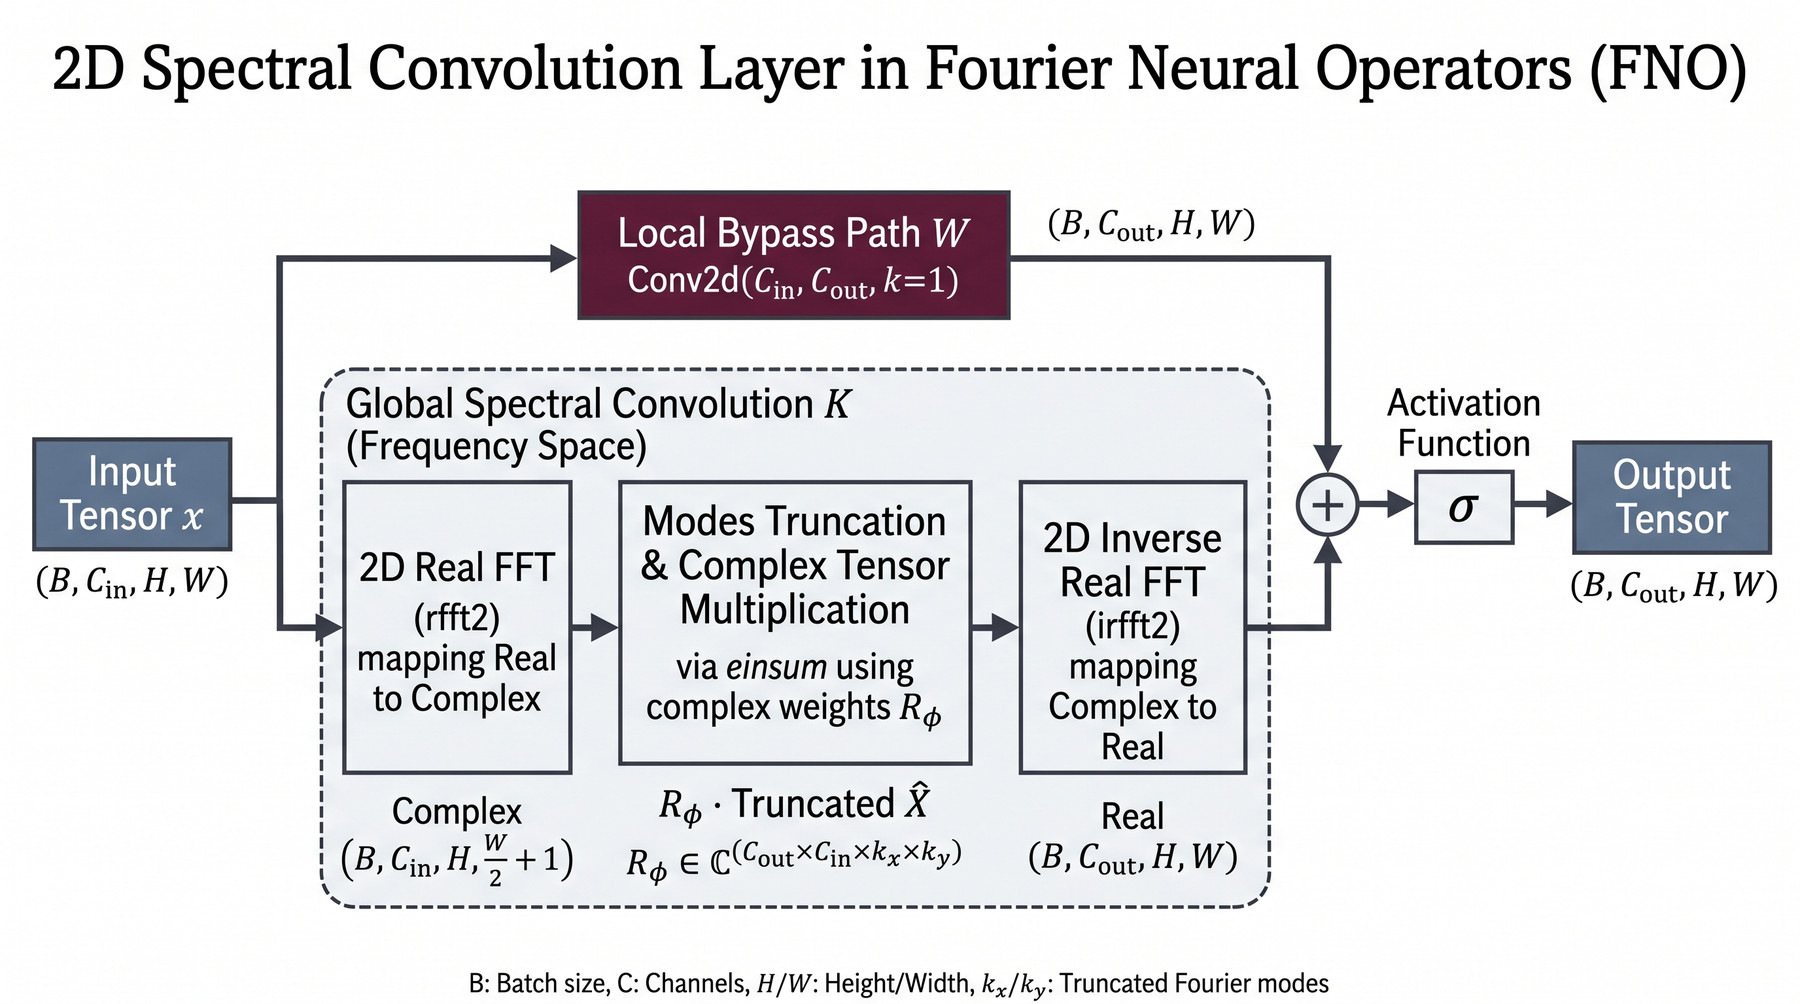
\includegraphics[width=0.95\textwidth]{fig_fno_spectral_layer.jpg}
\caption{\textbf{Architecture of the 2D Spectral Convolution Layer.} Input field $x$ splits into a local linear bypass $W x$ and a global spectral convolution $\mathcal{K} x$. The spectral branch computes the 2D real fast Fourier transform (FFT), slices the lowest $m_x \times m_y$ frequency modes, performs complex matrix multiplication via the learned parameter tensor $R_\phi$, zero-pads to the original grid shape, and reconstructs the physical representation via the inverse real FFT. Shapes at each stage are those of Listings~\ref{lst:ch23-spectral-conv2d} and~\ref{lst:ch23-fno2d}; the figure's legend denotes the retained mode counts by $k_x, k_y$, this book's text writes them $m_x, m_y$, and the code writes them \texttt{modes1}, \texttt{modes2}. The figure lists $R_\phi$ with the channel axes in the order $C_{\text{out}} \times C_{\text{in}}$; \eqref{eq:ch23-Rtensors} and the \texttt{einsum} subscript of Listing~\ref{lst:ch23-spectral-conv2d} fix the opposite order, and agree with each other.}
\label{fig:fno_spectral}
\end{figure}

Start with the transform. For a real input field
$x \in \mathbb{R}^{B \times C_{\text{in}} \times H \times W}$, its 2D
real-valued discrete Fourier transform is
\index{real-to-complex Fourier transform (rfft2)}
\begin{equation}
  \label{eq:ch23-rfft2}
  \hat{x} = \text{\texttt{torch.fft.rfft2}}(x) \in \mathbb{C}^{B \times C_{\text{in}} \times H \times (\lfloor W/2 \rfloor + 1)}.
\end{equation}
The call is the \emph{real-to-complex} FFT of the last two axes; the leading
batch and channel axes are carried along as transform batches, so one call
transforms the whole tensor rather than looping over fields. Two consequences
follow from the name. Because the input is real, conjugate symmetry holds:
$\hat{x}(-k_x, -k_y) = \overline{\hat{x}(k_x, k_y)}$, and the half-complex
representation in dimension $W$ fully determines the field --- the routine
returns $\lfloor W/2 \rfloor + 1$ coefficients along the last axis instead of
$W$, and the inverse \texttt{irfft2} reconstructs the omitted half from the
symmetry rather than from stored data. The second consequence is a budget
statement: a half-spectrum costs $2(\lfloor W/2 \rfloor + 1) \approx W$ real
values per row, which is what the real input already occupied, where a full
complex spectrum would cost twice that. Choosing \texttt{rfft2} over
\texttt{fft2} is therefore not a micro-optimization; it is what keeps the
frequency-domain intermediate no larger than the physical one.
\index{Fourier transform!real-to-complex, memory parity}

Parameterizing the convolution kernel begins by retaining the lowest $m_x$ and
$m_y$ modes. The retained set is a union of two contiguous blocks, called the
upper and lower corners in the comments of
Listing~\ref{lst:ch23-spectral-conv2d}:
\index{mode slicing!two-corner retention}
\begin{equation}
  \label{eq:ch23-corners}
  \begin{aligned}
  Z_m = \big\{(k_x, k_y): {}& k_x \in [0, m_x-1],\; k_y \in [0, m_y-1]\big\} \\
  \cup\; \big\{(k_x, k_y): {}& k_x \in [H - m_x, H-1],\; k_y \in [0, m_y-1]\big\}.
  \end{aligned}
\end{equation}
The two blocks are not ``low'' and ``high'' in the sense of one being more
oscillatory than the other. Under the usual ordering of FFT output, indices
$0, \dots, m_x - 1$ along the $H$ axis are the nonnegative small wavenumbers,
while indices $H - m_x, \dots, H - 1$ are the same wavenumbers taken with
negative sign; both are low in $|k_x|$. What makes the pair natural is
\eqref{eq:ch05-reality}: the conjugate of a mode with $k_y < 0$ is a mode with
$k_y > 0$, so storing the $k_y \ge 0$ half of the box and letting the inverse
transform supply the rest loses nothing. That is precisely the implementation
strategy Part~I announced when it observed that a real-output layer needs
weights for only half the modes and that this is the origin of two paired
weight tensors. The book-keeping is now explicit: \eqref{eq:ch23-corners} holds
$2 m_x m_y$ modes, against $(2m_x+1)(2m_y+1) \approx 4m_xm_y$ for the full box
$Z_{k_{\max}}$ of \eqref{eq:ch05-modeset}, and the factor of two is exactly the
one conjugacy buys, up to the self-conjugate line $k_y = 0$.

Two complex weight tensors are parameterized:
\begin{equation}
  \label{eq:ch23-Rtensors}
  R^{(1)} \in \mathbb{C}^{C_{\text{in}} \times C_{\text{out}} \times m_x \times m_y}, \qquad R^{(2)} \in \mathbb{C}^{C_{\text{in}} \times C_{\text{out}} \times m_x \times m_y}.
\end{equation}
\index{complex weight tensors}
Read \eqref{eq:ch23-Rtensors} against \eqref{eq:ch05-multiplier} and the
correspondence is one matrix per retained wavenumber: the continuum layer
carries $R_\phi(k) \in \mathbb{C}^{d_v \times d_v}$, and here those matrices
are stacked into two arrays whose last two indices enumerate the retained modes
of \eqref{eq:ch23-corners} and whose first two enumerate the channel rotation
applied at each of them. The one liberty is the order of those first two
indices: the arrays are stored with the input channel first, so each slice is
the transpose of the continuum matrix acting on a column of channel
coefficients. That convention is fixed by the \texttt{einsum} subscript below,
and it is the opposite of the one written on the figure. Note what is absent
from the shapes:
neither $H$ nor $W$ appears. The learnable parameters of a spectral layer do not
know the resolution they are applied to, which is the concrete form the
grid-independence of \eqref{eq:ch09-paramcount} takes in code.

Listing~\ref{lst:ch23-spectral-conv2d} is the complete layer. Its constructor
draws both arrays from a uniform distribution on $[0,1)$ scaled by
$1/(C_{\text{in}}C_{\text{out}})$ --- a small initialization, and an unusual one
in that its mean is positive. Every entry of every retained
mode therefore starts with the same sign, and the expected sum over input
channels at one output channel is
$C_{\text{in}}/(2C_{\text{in}}C_{\text{out}}) = 1/(2C_{\text{out}})$: on a
constant channel vector the spectral branch begins as a contraction, and must
learn its gain. In the forward pass, the line that
allocates
\texttt{out\_ft} as zeros is load-bearing twice over: it places the output
tensor on the input's device with the correct dtype, and it makes every mode
outside $Z_m$ identically zero, so the spectral branch is band-limited by
construction and truncation is a property of the data path rather than a penalty
term. The multiplication itself uses \texttt{torch.einsum} --- the Einstein
summation convention, in which a subscript appearing on both inputs and not on
the output is contracted --- with the pattern \texttt{"bixy,ioxy->boxy"}. The
letters name batch $b$, input channel $i$, output channel $o$, and the two mode
indices $x, y$; $i$ is summed, so at each retained mode $(x, y)$ the operation
is one matrix--vector product $C_{\text{out}} \times C_{\text{in}}$ against the
channel vector of coefficients at that mode. Nothing in the pattern carries a
term coupling $(x,y)$ to a different $(x',y')$, which is the code's version of
the diagonalization \eqref{eq:ch05-convolution-theorem} establishes.
\index{Einstein summation convention (einsum)}
\index{channel mixing!per-mode matrix product}

\begin{lstlisting}[language=Python, caption={\texttt{SpectralConv2d}: the 2D Fourier spectral convolution of \eqref{eq:ch23-rfft2}--\eqref{eq:ch23-Rtensors} in full. Its four commented stages map onto the three boxes of Figure~\ref{fig:fno_spectral}; the second stage, allocating the zeroed output tensor, is the zero-padding that figure's caption mentions rather than a box of its own.}, label={lst:ch23-spectral-conv2d}]
import torch
import torch.nn as nn

class SpectralConv2d(nn.Module):
    """2D Fourier Spectral Convolution Layer using complex matrix multiplication."""
    def __init__(self, in_channels: int, out_channels: int, modes1: int, modes2: int):
        super().__init__()
        self.in_channels = in_channels
        self.out_channels = out_channels
        self.modes1 = modes1 # Frequency modes along height H
        self.modes2 = modes2 # Frequency modes along width W

        # Complex weights initialized with uniform scaling
        scale = 1.0 / (in_channels * out_channels)
        self.weights1 = nn.Parameter(
            scale * torch.rand(in_channels, out_channels, self.modes1, self.modes2, dtype=torch.cfloat)
        )
        self.weights2 = nn.Parameter(
            scale * torch.rand(in_channels, out_channels, self.modes1, self.modes2, dtype=torch.cfloat)
        )

    def forward(self, x: torch.Tensor) -> torch.Tensor:
        # Input shape: (B, C_in, H, W)
        B, C, H, W = x.shape
        
        # 1. Compute 2D Real FFT: Output shape (B, C_in, H, W//2 + 1)
        x_ft = torch.fft.rfft2(x)
        
        # 2. Allocate complex output tensor in frequency domain
        out_ft = torch.zeros(B, self.out_channels, H, W // 2 + 1, device=x.device, dtype=torch.cfloat)
        
        # 3. Multiply retained Fourier modes by complex weight tensors
        # Upper corner: kx in [0, modes1), ky in [0, modes2)
        out_ft[:, :, :self.modes1, :self.modes2] = torch.einsum(
            "bixy,ioxy->boxy", x_ft[:, :, :self.modes1, :self.modes2], self.weights1
        )
        # Lower corner: kx in [-modes1, 0), ky in [0, modes2)
        out_ft[:, :, -self.modes1:, :self.modes2] = torch.einsum(
            "bixy,ioxy->boxy", x_ft[:, :, -self.modes1:, :self.modes2], self.weights2
        )
        
        # 4. Compute 2D Inverse Real FFT to return to physical domain
        x_out = torch.fft.irfft2(out_ft, s=(H, W))
        return x_out
\end{lstlisting}

% -----------------------------------------------------------------------------
\section{Cost, Parameter Count, and Failure Behavior of the Layer}
\label{sec:ch23-cost-and-failure}
% -----------------------------------------------------------------------------

Two remarks on the last line of Listing~\ref{lst:ch23-spectral-conv2d} before the
cost tally. The first concerns
resolution, and it does not come from the argument \texttt{s} but from the line
that reads \texttt{B, C, H, W} off the incoming tensor: every index in
\eqref{eq:ch23-corners} addresses a \emph{mode}, not a grid point, so handing the
same weights a $256 \times 256$ field evaluates the same band-limited multiplier
on a finer set of nodes. That is the code path behind
Proposition~\ref{prop:ch06-zeroshot}, with its caveat intact --- the identity is
exact for inputs already resolved on the training grid, and for nothing else.
The role of \texttt{s=(H, W)} is narrower and easily misread: a half-spectrum
with $\lfloor W/2 \rfloor + 1$ columns is compatible with two input widths, one
even and one odd, so the target shape has to be stated rather than inferred.
The second remark concerns normalization. PyTorch's forward transform is
unnormalized and its inverse divides by
$HW$, and the two factors cancel exactly across the pair. The learned array is
therefore the continuum multiplier $R_\phi(k)$ of \eqref{eq:ch05-multiplier},
apart from the transposition noted after \eqref{eq:ch23-Rtensors}, and not $HW$
times it; no grid-dependent rescaling of the weights is needed when the
grid changes, which is the numerical reason the parameter vector means the same
object on every mesh.

Counting operations per layer, for a batch of $B$ fields on an $H \times W$
grid,
\begin{equation}
  \label{eq:ch23-cost}
  \underbrace{5\,B\,(C_{\text{in}} + C_{\text{out}})\,HW \log_2(HW)}_{\text{forward and inverse transforms}}
  \;+\;
  \underbrace{6 \cdot 2\, B\, m_x m_y\, C_{\text{in}} C_{\text{out}}}_{\text{complex multiply--adds on } Z_m}
  \quad \text{floating-point operations},
\end{equation}
where $5N\log_2 N$ is the customary estimate for one complex transform of $N$
points, charged once over the $B C_{\text{in}}$ fields going in and once over
the $B C_{\text{out}}$ coming out, on an $H \times W$ array whose row and column
passes together give $\log_2 H + \log_2 W = \log_2(HW)$; and where a complex
multiply--add costs six real operations over the $2m_xm_y$ retained modes of
\eqref{eq:ch23-corners}. The first term overstates the real-to-complex pair by
roughly a factor of two, since a transform with a real input does about half the
work of a complex one of the same size; it is left in that form so that the
comparison below is conservative.
\index{computational cost!spectral layer, per-term}
Equation \eqref{eq:ch23-cost} is the operational content of the FNO line of
\eqref{eq:ch8-costs}, $\Theta(d_v N \log N + K d_v^2)$, with $K = 2m_xm_y$. Its
two halves behave very differently under refinement, and that asymmetry is the
argument: the learned arithmetic is the second term, which does not grow with
$H$ or $W$ at all, so refining the grid from $64^2$ to $256^2$ multiplies the
transform term by about $21$ --- a little more than the factor of $16$ in points,
because of the logarithm --- against the $256$ a dense discretization of
\eqref{eq:fredholm_kernel} would demand. At $64^2$ with $32$ channels and a
$12 \times 12$ band, the multiplier performs
$2 \cdot 144 \cdot 32 \cdot 32 \approx 3 \times 10^{5}$ complex multiply--adds
per field, while the dense alternative stores and applies an
$(HW)^2 \approx 1.7 \times 10^{7}$ kernel array per channel pair. The
$\mathcal{O}(N \log N)$ of
\chapref{ch:part1-the-fourier-neural-operator-spectral-theor} has become an
addressable object: it is the first term, and everything learnable sits in the
second.

The parameter count follows from \eqref{eq:ch23-Rtensors} directly,
\begin{equation}
  \label{eq:ch23-paramcount}
  P_{\text{spec}} = 2\, m_x m_y\, C_{\text{in}} C_{\text{out}} \ \text{complex} = 4\, m_x m_y\, C_{\text{in}} C_{\text{out}} \ \text{real}.
\end{equation}
For the reference two-dimensional configuration --- width
$C_{\text{in}} = C_{\text{out}} = 32$, band $m_x = m_y = 12$, depth $4$ ---
\eqref{eq:ch23-paramcount} gives $5.9 \times 10^{5}$ real numbers per spectral
layer and $2.4 \times 10^{6}$ across the stack: a few million parameters, set
entirely by the band and the width, with no term in $H$ or $W$ anywhere. The same
arithmetic explains why mode counts in practice sit at a dozen to sixteen per
direction: past the point where the algebraic truncation curve of
Figure~\ref{fig:spectral_decay} falls below the network's own error --- a term
that figure computes nothing about ---
widening $Z_m$ adds parameters without adding accuracy.
\index{parameter count!of a spectral layer}
\index{mode budget!reference configuration}

What breaks, and how loudly? The slicing convention of
\eqref{eq:ch23-corners} is the fragile part. If \texttt{modes2} exceeds
$\lfloor W/2 \rfloor + 1$, the slice returns fewer columns than
\texttt{weights1} has and \texttt{einsum} raises a shape error --- a loud,
immediately diagnosable failure. If instead $2\,\texttt{modes1} > H$ while
$\texttt{modes1} \le H$, both slices are well-formed, they overlap on the rows
$[H - \texttt{modes1},\, \texttt{modes1})$, and the second assignment silently
overwrites the first there. The layer still runs, still returns a tensor of the
right shape, and no longer computes the multiplier intended on the overlapping
modes. The safeguard is a constraint, not a check: keep $2m_x < H$ and
$m_y \le \lfloor W/2 \rfloor + 1$, which is the Nyquist-type hypothesis
$N_{\text{train}} > 2k_{\max}$ of Proposition~\ref{prop:ch06-zeroshot}
reappearing as a sanity bound on a configuration file.
\index{index slicing!overlap failure}

% -----------------------------------------------------------------------------
\section{Full FNO-2D Model Architecture}
\label{sec:ch23-fno2d}
% -----------------------------------------------------------------------------

The spectral layer is one stage of a network. Written as an operator on grid
fields, the assembled model is the discrete reading of \eqref{eq:fno_layer}
together with the composition \eqref{eq:no_composition}:
with $\mathcal{F}_N$ and $\mathcal{F}_N^{-1}$ the transform pair of
\eqref{eq:ch23-rfft2} and $R_\phi^{(N)}$ supported on $Z_m$ as in
\eqref{eq:ch23-corners},
\begin{equation}
  \label{eq:ch23-layer}
  v_{\ell+1} = \sigma\Big( W_\ell v_\ell + \mathcal{F}_N^{-1}\big( R_\phi^{(N)} \odot \mathcal{F}_N v_\ell \big) \Big),
  \qquad
  \mathcal{G}_\theta = \mathcal{Q} \circ \mathcal{V}^{(N)}_L \circ \cdots \circ \mathcal{V}^{(N)}_1 \circ \mathcal{P},
\end{equation}
where $\mathcal{V}^{(N)}_\ell$ is the map the left-hand display defines, taking
grid samples of $v_\ell$ to grid samples of $v_{\ell+1}$.
\index{FNO-2D!layer recursion}
The full network wraps the spectral convolutions between a local lifting
multilayer perceptron (MLP) $\mathcal{P}$ and a projection MLP $\mathcal{Q}$, and
Listing~\ref{lst:ch23-fno2d} is that construction in full. Three details of the
listing carry the design.

\begin{lstlisting}[language=Python, caption={The complete FNO-2D of \eqref{eq:ch23-layer}: grid embedding, pointwise lifting, a stack of spectral blocks with local bypass, and pointwise projection.}, label={lst:ch23-fno2d}]
class FNO2d(nn.Module):
    """Full 2D Fourier Neural Operator with stacked spectral-convolution layers."""
    def __init__(self, in_channels: int, out_channels: int, modes1: int, modes2: int, 
                 hidden_channels: int = 32, n_layers: int = 4):
        super().__init__()
        self.grid_embed = GridEmbeddingND(dim=2)
        
        # Lifting: maps (C_in + 2) channels to hidden dimension
        self.p = nn.Conv2d(in_channels + 2, hidden_channels, kernel_size=1)
        
        # Stack of Fourier operator layers
        self.spectral_layers = nn.ModuleList([
            SpectralConv2d(hidden_channels, hidden_channels, modes1, modes2)
            for _ in range(n_layers)
        ])
        self.ws = nn.ModuleList([
            nn.Conv2d(hidden_channels, hidden_channels, kernel_size=1)
            for _ in range(n_layers)
        ])
        
        # Projection: maps hidden dimension back to C_out channels
        self.q = nn.Sequential(
            nn.Conv2d(hidden_channels, 128, kernel_size=1),
            nn.GELU(),
            nn.Conv2d(128, out_channels, kernel_size=1)
        )
        self.act = nn.GELU()

    def forward(self, x: torch.Tensor) -> torch.Tensor:
        # Append positional grid coordinates
        x = self.grid_embed(x)
        x = self.p(x) # Shape: (B, hidden_channels, H, W)
        
        for spec_conv, w_conv in zip(self.spectral_layers, self.ws):
            # Parallel spectral and local bypass paths
            x1 = spec_conv(x)
            x2 = w_conv(x)
            x = self.act(x1 + x2)
            
        x = self.q(x) # Shape: (B, out_channels, H, W)
        return x
\end{lstlisting}

First, the lifting convolution takes \texttt{in\_channels + 2} inputs. The extra
two are the normalized coordinate channels appended by \texttt{GridEmbeddingND},
the utility of \chapref{ch:part2-the-practitioner-s-paradigm-infinite-dimen}
that turns a field into $a_{\text{augmented}} = [a, x_1, x_2]$.
\index{coordinate channels!in FNO lifting}
The consequence is easy to misdescribe.
The coordinate channels are not carried through as geometry: lifting mixes them
into the hidden channels, and from that point on they are transformed and
truncated like everything else. What they contribute is a location. Every
operation in \eqref{eq:ch23-layer} is equivariant to translations on the torus
--- that is precisely what the diagonalization \eqref{eq:ch05-convolution-theorem}
buys --- so a network fed only field values cannot distinguish a feature at $x$
from the same feature at $x + h$. Appending $x_1$ and $x_2$ is the cheap way to
break that symmetry, and it is the translational ambiguity of
\chapref{ch:part2-the-practitioner-s-paradigm-infinite-dimen} seen from the
inside of a forward pass.

Second, both $\mathcal{P}$ and $\mathcal{Q}$ are built from $1 \times 1$
convolutions, which are pointwise maps. The lift in the listing is a single such
convolution --- the degenerate case of the shallow MLP that
\eqref{eq:no_composition} permits --- while the projection is a two-layer
stack, $C_{\text{hid}} \to 128 \to C_{\text{out}}$ through a Gaussian error
linear unit (GELU). Both act independently at every grid point, so all spatial
communication in the model happens in the spectral branch or in the bypass, and
the input and output resolutions are identical --- the network is grid-to-grid,
and no interpolation stage appears anywhere in \eqref{eq:ch23-layer}.

Third, and most substantive: why keep $W_\ell$ at all, when the spectral branch
already performs a global learned operation? The answer is a limitation of
\eqref{eq:ch23-layer} that the code makes visible. The spectral branch maps its
input into the band-limited subspace spanned by $Z_m$ and discards everything
else; the pointwise $W_\ell$ is the only path by which content outside the band
reaches layer $\ell + 1$ intact. Without it, information above the cutoff could
survive only by being folded down through the nonlinearity --- $\sigma$ applied
to a band-limited field generates harmonics outside the band, which the next
layer truncates again --- a lossy and poorly controlled route. The bypass is thus
the price of truncation, not redundancy: it is what lets a twelve-mode layer
still be a map on fields rather than a map on twelve-mode
approximations.
\index{local bypass convolution!necessity}

Grid-independence also fixes the bias. \chapref{ch:part1-the-fourier-neural-operator-spectral-theor}
writes \eqref{eq:fno_layer} with a bias $b_\ell(x)$ that is a function of
position. In the listing, the bias is the default \texttt{bias} of
\texttt{nn.Conv2d}: one constant per output channel, shared across all $HW$
locations. That is a deliberate specialization, and a necessary one. A bias
attached to grid points would add $HW$ learnable numbers per channel, the
parameter array would acquire a shape dependent on the discretization, and the
grid-independence visible in \eqref{eq:ch23-Rtensors} --- and asserted by
\eqref{eq:ch09-paramcount} --- would be forfeited. Part~I excludes such an
architecture on exactly those grounds; here is the exclusion implemented.
\index{bias!pointwise versus grid-attached}

Tracing shapes through the forward pass fixes the rest of the accounting. A batch
of scalar fields arrives as $(B, 1, H, W)$, becomes $(B, 3, H, W)$ after grid
embedding, $(B, C_{\text{hid}}, H, W)$ after lifting, and stays at
$(B, C_{\text{hid}}, H, W)$ through all $L$ blocks --- the architecture is a
width-preserving stack with no pooling, no striding, and no upsampling, which is
what distinguishes it structurally from a convolutional encoder--decoder.
Each block holds a spectral array counted by \eqref{eq:ch23-paramcount} and a
bypass of $C_{\text{hid}}^2 + C_{\text{hid}}$ parameters, so at
$C_{\text{hid}} = 32$
the bypass contributes under one percent of the block's parameters while
contributing all of its spatially unresolved behavior. Memory, however, follows
the frequency tensor, not the parameter count: at $B = 16$,
$C_{\text{hid}} = 32$ and $H = W = 64$, both \texttt{x\_ft} and
\texttt{out\_ft} occupy $16 \cdot 32 \cdot 64 \cdot 33 \approx 1.1 \times 10^{6}$
complex entries, about $8.7$ MB in fp32-complex each, and an autograd-enabled
forward pass retains both per layer --- roughly $70$ MB of frequency-domain
intermediates for a four-layer stack before counting anything else. Those are
fp32 figures; the case for running parts of the network in bfloat16, and the
reason the transform and the complex multiplication are the last places one
applies automatic mixed precision (AMP), is taken up in
\chapref{ch:part2-training-regimes-optimization-and-failure-}.
\index{memory footprint!frequency-domain intermediates}
\index{automatic mixed precision (AMP)}

% -----------------------------------------------------------------------------
\section{Using the Official \texttt{neuraloperator} Library}
\label{sec:ch23-library}
% -----------------------------------------------------------------------------

Everything above is under a hundred lines of PyTorch, and a reader should be
able to write it, read it, and debug it. Production use is a different matter.
The official \texttt{neuraloperator} library maintained by Caltech and NVIDIA
provides industrial-grade implementations, including a factorized variant --- the
\texttt{TFNO} class that the workflow of
Listing~\ref{lst:ch23-neuraloperator-workflow} instantiates --- in which the
multiplier arrays of \eqref{eq:ch23-Rtensors} are stored through a Tucker or
CANDECOMP/PARAFAC (CP) tensor decomposition instead of as dense arrays, which
compresses the parameter store without changing the arithmetic of
\eqref{eq:ch23-layer}.
\index{neuraloperator library}
\index{tensor factorization!of spectral multiplier arrays}
\index{CANDECOMP/PARAFAC (CP) decomposition}

The mechanism of that compression is worth stating, because it is the one place
where the library departs from the parameterization \eqref{eq:ch23-Rtensors} in
a way that earns its keep. \eqref{eq:ch23-Rtensors} stores the mode-indexed channel
rotations as a four-way array and spends \eqref{eq:ch23-paramcount} parameters
on it; a Tucker decomposition replaces the array by a small core tensor
contracted with one factor matrix along each axis, and a
CP decomposition replaces it by a sum of rank-one terms
\index{Tucker decomposition!in a factorized spectral layer}
--- the multilinear reconstruction \eqref{eq:ch8-tucker} of
\chapref{ch:part1-comparative-theoretical-taxonomy-of-archit}, drawn there with
the mode index flattened into a single axis and four-way here because
\eqref{eq:ch23-Rtensors} keeps the two spatial mode axes distinct. What changes
is which products appear. \eqref{eq:ch8-tucker} costs a term linear in the band
size times the mode rank, plus terms linear in each channel width, where
\eqref{eq:ch23-paramcount} pays the band size times \emph{both} channel widths
at once; widening the band --- which is what buys accuracy when the target's
regularity is low, per \eqref{eq:ch05-error-decomposition} --- therefore costs
one extra rank's worth of parameters per mode instead of
$C_{\text{in}}C_{\text{out}}$ worth. How much any particular configuration saves
is thus fixed by the rank chosen against the band and the channel widths entered
in \eqref{eq:ch23-paramcount}, not by the factorization as such: the two counts
can be subtracted by hand on any configuration, and the \texttt{rank=0.42} of
Listing~\ref{lst:ch23-neuraloperator-workflow} is one illustration of the
trade; the percentage annotated on that line describes
that example alone and is not a compression factor this book reports. Compression is not free, however, and Part~I is explicit about
the price: the ranks must genuinely be small for the count to fall, and whether
the multiplier arrays a solution operator induces are low-rank is an empirical
premise that no theorem here supports. Factorizing constrains
\eqref{eq:ch23-Rtensors} to a low-rank manifold that
\eqref{eq:ch05-error-decomposition} does not account for, so band and rank trade
off in a way the theory leaves to the validation curve.

\begin{lstlisting}[language=Python, caption={The canonical training workflow of the official \texttt{neuraloperator} library: a factorized model, the relative-$L^p$ loss, and the optimizer, assembled as three independent objects.}, label={lst:ch23-neuraloperator-workflow}]
from neuralop.models import FNO, TFNO
from neuralop import LpLoss
from neuralop.training import AdamW

# Instantiate Tensorized FNO (TFNO) for high memory efficiency
model = TFNO(
    n_modes=(16, 16),
    in_channels=1,
    out_channels=1,
    hidden_channels=64,
    factorization='tucker',
    rank=0.42 # Compresses complex parameter tensor by 58%
).cuda()

loss_fn = LpLoss(d=2, p=2)
optimizer = AdamW(model.parameters(), lr=8e-3, weight_decay=1e-4)
\end{lstlisting}

Listing~\ref{lst:ch23-neuraloperator-workflow} is the workflow, and comparing it
line by line with Listings~\ref{lst:ch23-spectral-conv2d}
and~\ref{lst:ch23-fno2d} shows what the library keeps and what it changes. The
object model is the same. The pair \texttt{modes1} and \texttt{modes2} reappears
as \texttt{n\_modes}, the hidden width keeps the name \texttt{hidden\_channels},
and the input and output channel counts are both $1$ --- the Darcy
coefficient-to-pressure map of \eqref{eq:darcy}, scalar input, scalar output,
same grid in and out. What the library adds is the machinery a from-scratch file
leaves implicit: the factorization keyword, device placement made explicit by a
\texttt{.cuda()} call on the whole module, and a loss and an optimizer that
arrive as separate objects. Two of those differences bear on the computation.
The library's \texttt{LpLoss} takes an
explicit spatial-dimension argument \texttt{d=2}, because it forms a
quadrature-weighted norm of the kind in \eqref{eq:rel_l2_loss} rather than a
plain vector norm over flattened data; on an equispaced grid the weights cancel
in the ratio and the two coincide, which is exactly why the from-scratch version
of \chapref{ch:part2-the-practitioner-s-paradigm-infinite-dimen} is safe there.
A weighted implementation keeps its meaning when the quadrature is nonuniform
or when the norm mixes terms of different differential order. And
\texttt{AdamW} --- Adam with decoupled weight decay --- is imported from the library's own training module, though \texttt{torch.optim}
provides its own implementation, so that a question the from-scratch file never has
to answer is settled
once, for every user:
what decay applied to the complex arrays of \eqref{eq:ch23-Rtensors} acts on,
their magnitudes or their real and imaginary parts separately.
\index{AdamW optimizer}
\index{relative $L^2$ loss!quadrature-weighted variant}

The learning rate of \texttt{lr=8e-3} should be read with care. It is an initial
value, not a recommendation to train at a constant rate: because complex
Fourier multipliers act directly on the frequency modes, holding a rate of this
size fixed produces early training instability, and the schedule that makes such
a rate usable --- one-cycle ramping, gradient clipping, and the weight decay
already visible above --- is the subject of
\chapref{ch:part2-training-regimes-optimization-and-failure-}. Likewise, the
model returned by \texttt{TFNO(...).cuda()} is trained and evaluated by exactly
the arithmetic of \eqref{eq:ch23-layer}; what the library does not do is choose
the band. That choice, made in \eqref{eq:ch23-corners} and argued in
\chapref{ch:part1-the-fourier-neural-operator-spectral-theor}, remains the
practitioner's, and it remains the single hyperparameter whose effect on accuracy
the theory actually predicts.
\index{hyperparameters!mode budget as the predicted one}

% -----------------------------------------------------------------------------
\medskip
The layer written here buys its $\mathcal{O}(N \log N)$ cost with three
purchases: a periodic torus, a stationary kernel, and a fixed band. The first is
the binding one for everything this book will later simulate. External
aerodynamics over a car body, flow through a faulted porous reservoir, and
electrophysiology on a ventricle do not live on $[0,1)^2$, and no amount of
padding or masking makes a tensor-product grid conform to a boundary that curves
through it. \index{Fourier neural operator!limitations of, periodic domains}
Neither is the truncation of \eqref{eq:ch23-corners} available, since on an
unstructured mesh there is no transform whose output axes a slice could address.
\chapref{ch:part2-graph-neural-operators-gno-and-irregular-g}
therefore abandons diagonalization and returns to the Fredholm kernel
\eqref{eq:fredholm_kernel} in its unspecialized form, evaluating it by local
quadrature over neighborhoods rather than globally over frequencies: the graph
neural operator (GNO), whose per-layer cost $\Theta(|E| d_v^2)$ in
\eqref{eq:ch8-costs} is set by the number of mesh edges instead of the number of
grid points, and whose implementation is the subject of that chapter's first
half. The two architectures are not rivals but complements, and its second half
composes them: the geometry-informed neural operator (GINO) puts graph layers at
either end of a latent spectral stack, leaving the mesh, doing the fast global
work in frequency space, and returning.

% Chapter 13: Graph Neural Operators (GNO) and Irregular Geometries
% Part II of the book.

\chapter{Graph Neural Operators (GNO) and Irregular Geometries}
\label{ch:part2-graph-neural-operators-gno-and-irregular-g}
\label{sec:gno}
% -----------------------------------------------------------------------------

The spectral construction of \chapref{ch:part1-the-fourier-neural-operator-spectral-theor} is
exact where it is cheap, and cheap only where it is exact. Its kernel is a function of the
difference $x-y$, and its integrals are evaluated by the discrete Fourier transform, so both
the convolution theorem and the $\mathcal{O}(N \log N)$ cost of a layer presuppose a lattice:
a uniform grid on the periodic torus $\mathbb{T}^{d}$. Most engineering geometry is not that.
The surface of an airframe, a pump housing, or a ventricle arrives as a triangulated mesh with
irregular node spacing, no translational symmetry, and a node count that changes whenever a
designer nudges a control point
\index{unstructured mesh}\index{partial differential equation (PDE)!on complex geometries}.
Viscous flow, structural mechanics, and cardiovascular simulations are then governed by
partial differential equations (PDEs) on such surfaces, and the Fourier machinery of
\chapref{ch:part2-fourier-neural-operators-fno-from-scratch} does not apply until something
has been said about how a mesh enters a network.

This chapter says it. The object that survives without a lattice is the integral-kernel layer
\eqref{eq:no_layer} of the generic neural operator \cite{kovachki2023neural}: the trainable
Fredholm kernel \eqref{eq:fredholm_kernel} that the ledger of
\index{generic neural operator!implementation in Part II}Table~\ref{tab:ch8-ledger} assigns to
this chapter, because no other Part~II chapter builds one. The \emph{graph neural operator} (GNO)
keeps that kernel and restricts its \emph{support} rather than its algebraic form; the
\emph{geometry-informed neural operator} (GINO) composes such layers with a Fourier operator
acting on an auxiliary regular grid \cite{li2023geometry}, along the lines written out in
\eqref{eq:ch8-gino} and costed in \eqref{eq:ch8-costs}. Three things break in the move and
each is repaired below: the transform itself, since a mesh admits no $\mathcal{O}(N \log N)$
convolution; the batch, since two tessellations of two bodies have different node counts where
a grid at least shares its shape; and the quadrature, since the spacing factor $\Delta x$ of a
grid sum must be replaced by per-node weights derived from the mesh.

The reader should bring PyTorch \cite{paszke2019pytorch}, the tensor layouts of
\chapref{ch:part2-the-practitioner-s-paradigm-infinite-dimen}, and the spectral layer of
\chapref{ch:part2-fourier-neural-operators-fno-from-scratch}; and the vocabulary of computing
on a graphics processing unit (GPU) --- device-resident tensors, kernel launches, atomic
updates, and the CUDA (Compute Unified Device Architecture) Deep Neural Network library
(cuDNN) --- since the costs here are dominated by memory traffic rather than arithmetic.
Nothing new is proved. \chapref{ch:part1-comparative-theoretical-taxonomy-of-archit} records
no convergence rate and no discretization-invariance theorem for either architecture, and this
chapter does not supply one; what it supplies is the layer, the pipeline, and an honest
accounting of what the geometry buys and what it costs.

% -----------------------------------------------------------------------------
\section{The Continuous Kernel Graph Convolution}
\label{sec:ch24-continuous-kernel}
% -----------------------------------------------------------------------------

A GNO layer \cite{li2023geometry} parameterizes a non-local Fredholm integral kernel over an
arbitrary spatial discretization:
\begin{equation}
  \label{eq:ch24-gno-kernel}
  (\mathcal{K} v)(x_i) = \int_{\mathcal{B}_r(x_i)} \kappa_\theta(x_i, y) \, v(y) \, dy \approx
  \sum_{j \in \mathcal{N}_r(i)} \kappa_\theta(x_i - x_j, \, a(x_i), \, a(x_j)) \, v(x_j) \, w_j,
\end{equation}
where $\mathcal{B}_r(x_i)$ is the ball of radius $r$ about $x_i$,
\index{Graph Neural Operator (GNO)!neighborhood radius} $\mathcal{N}_r(i) = \{j : \|x_i -
x_j\| \le r\}$ is the set of mesh nodes whose distance to node $i$ is at most $r$, and $w_j$
is the Voronoi dual area of vertex $j$ on the surface --- its tributary measure, the fraction
of the domain that a node speaks for
\index{Voronoi dual area}\index{Graph Neural Operator (GNO)!quadrature weights}. The kernel
$\kappa_\theta$ is a continuous multilayer perceptron (MLP) evaluated on relative coordinates
$\Delta x_{ij} = x_i - x_j$ and, in the general form of \eqref{eq:ch24-gno-kernel}, on the
input field at both endpoints.

Read \eqref{eq:ch24-gno-kernel} as quadrature before anything else. The left side integrates
against Lebesgue measure over a ball; the right side sums against the discrete measure $\sum_j
w_j \delta_{x_j}$ carried by the mesh. That is the same consistency condition Part~I imposed
in \eqref{eq:ch06-quadrature} and folded into the continuum-limit condition
\eqref{eq:limit_commute},
and it has a concrete consequence: on a quasi-uniform refinement of a surface, the tributary
area of a vertex shrinks like the square of the edge length while the number of nodes in a
fixed ball grows like the reciprocal of that square, so the sum holds its ground as an
approximation to the integral rather than drifting with mesh density. The weights are the
mesh's contribution to the layer. Everything else --- the kernel, the channel mixing, the
radius --- is the network's, and no parameter of it is indexed by a node.

The dependence on $a(x_i)$ and $a(x_j)$ deserves emphasis because it is the whole reason this
layer is an operator and not a mesh-bound convolution. The Fourier neural operator (FNO)
reaches its cost by discarding those arguments and imposing stationarity,
$\kappa_\ell(x,y,a(x),a(y);\phi_\ell) = \kappa_\ell(x-y;\phi_\ell)$, as in
\eqref{eq:ch8-fno-specialization} \cite{li2021fourier}. A GNO does not: an inhomogeneous or
input-dependent map can be approximated without the network having to smuggle the coefficient
field through side channels. Message-passing neural PDE solvers \cite{brandstetter2022message}
share the edge-based template but attach a learned update rule to each edge rather than a
kernel multiplying a quadrature weight \index{message passing}--- the distinction between a
learned stencil and a discretized integral, and it is what makes the graph layer a
specialization of \eqref{eq:no_layer}. The kernel row of
Table~\ref{tab:comparison} already books it against the generic operator's own
$\kappa_\theta(x,y)$, the geometric pair collapsed to a displacement, the input values at both
endpoints retained, and the domain of integration shrunk to a ball.

\begin{lstlisting}[language=Python, caption={One continuous-kernel graph convolution layer: a shared MLP maps each edge displacement to a channel-mixing matrix, and a scatter-add aggregation performs the unnormalized neighborhood sum defined in this section.}, label={lst:gno-kernel-conv}]
class KernelGraphConv(nn.Module):
    """Continuous-kernel graph convolution layer for irregular meshes."""
    def __init__(self, in_channels: int, out_channels: int, coord_dim: int = 3, hidden_dim: int = 64):
        super().__init__()
        # Continuous kernel MLP mapping displacement vectors to transformation matrices
        self.kernel_mlp = nn.Sequential(
            nn.Linear(coord_dim, hidden_dim),
            nn.GELU(),
            nn.Linear(hidden_dim, in_channels * out_channels)
        )
        self.in_channels = in_channels
        self.out_channels = out_channels

    def forward(self, v: torch.Tensor, coords: torch.Tensor, edge_index: torch.Tensor) -> torch.Tensor:
        """
        v:          (N_nodes, in_channels) - node feature representations
        coords:     (N_nodes, coord_dim) - 3D physical coordinates
        edge_index: (2, N_edges) - source and target node connectivity
        """
        src, dst = edge_index[0], edge_index[1]
        displacement = coords[dst] - coords[src] # Relative spatial vector (N_edges, coord_dim)
        
        # Evaluate continuous kernel weights at relative positions
        kernel_weights = self.kernel_mlp(displacement) # (N_edges, in_ch * out_ch)
        kernel_weights = kernel_weights.view(-1, self.in_channels, self.out_channels)
        
        # Message passing: transform node features
        v_src = v[src].unsqueeze(1) # (N_edges, 1, in_ch)
        messages = torch.bmm(v_src, kernel_weights).squeeze(1) # (N_edges, out_ch)
        
        # Neighborhood aggregation (scatter add)
        out = torch.zeros(coords.shape[0], self.out_channels, device=v.device)
        out.index_add_(0, dst, messages)
        return out
\end{lstlisting}

Listing~\ref{lst:gno-kernel-conv} is worth walking tensor shape by tensor shape, because the
shapes are where the design is legible. The connectivity arrives as \texttt{edge\_index}, an
integer tensor of shape $(2, N_{\text{edges}})$ whose two rows hold source and target node
indices --- the graph's sparse structure in the form a GPU can gather against
\index{edge index}\index{point-cloud layout}. From it, \texttt{displacement} is
$(N_{\text{edges}}, \texttt{coord\_dim})$, and the kernel MLP turns every displacement vector
into a full $\texttt{in\_channels} \times \texttt{out\_channels}$ matrix, so
\texttt{kernel\_weights} has shape $(N_{\text{edges}}, C_{\text{in}}, C_{\text{out}})$
\index{kernel MLP}. The batched matrix product \texttt{torch.bmm} then applies a
\emph{different} matrix to every edge, which is the arithmetic content of the sum in
\eqref{eq:ch24-gno-kernel}: $\Theta(|E|\,C_{\text{in}} C_{\text{out}})$ multiply-adds per
layer, the edge-linear count recorded in \eqref{eq:ch8-costs} as $\Theta(|E|\,d_v^{2})$. Two
features of the listing carry the operator semantics. First, no weight is indexed by node identity or by a lattice offset; the MLP is
shared across all edges, so refining the mesh multiplies the compute without multiplying the
parameters. Second, the aggregation is a \emph{scatter add} --- \texttt{index\_add\_} over the
target indices, unnormalized
\index{scatter-add aggregation}\index{computational complexity!graph convolution per edge}---
because \eqref{eq:ch24-gno-kernel} integrates rather than averages. Note honestly what the
listing does not do: it evaluates the kernel on the displacement alone, the stationary
reduction of \eqref{eq:ch24-gno-kernel}, and it carries no $w_j$. Both gaps are interface
obligations rather than bugs. Recovering the input-dependent kernel means concatenating
$a(x_i)$ and $a(x_j)$ into the MLP input, widening it from $\texttt{coord\_dim}$ to
$\texttt{coord\_dim} + 2C_{\text{in}}$; recovering the quadrature means folding the dual-area
weight into the node features or into the message before the scatter, since an unweighted sum
over a mesh of uneven spacing is a different functional from the one
\eqref{eq:ch24-gno-kernel} approximates.

Memory, not arithmetic, is the binding constraint. The per-edge matrices alone occupy $|E|
\times C_{\text{in}} \times C_{\text{out}}$ floating-point values: a million edges at 32
channels is $1.02 \times 10^{9}$ entries, roughly $4.1$~GB in single precision, and that is
one layer's intermediate. The channel width and the radius $r$ are therefore chosen against
the device's capacity, not against a parameter budget --- the parameters of
\eqref{eq:ch24-gno-kernel} live in an MLP whose size is independent of the mesh entirely.

Failure behavior follows from the same arithmetic and is worth stating before a training run
does it for you. If $r$ is small relative to the body, information crosses the geometry only
by composition: $\ell$ layers reach a distance $\ell r$, so spanning a body of diameter
$\operatorname{diam}(\Omega)$ costs on the order of $\operatorname{diam}(\Omega)/r$ layers,
the receptive-field arithmetic of
\chapref{ch:part1-comparative-theoretical-taxonomy-of-archit}
\index{receptive field!layers needed to span a body}. If $r$ is large, $|E|$ grows toward
$N^{2}$ and the layer quietly reverts to the dense-kernel operator and its $\Theta(N^{2})$
cost. Nodes in regions of high curvature or on a boundary accumulate different numbers of
incoming edges from nodes on a flat panel, and because the aggregation is unnormalized the
magnitude of the output scales with local node occupancy --- a systematic drift across layers,
not noise. Finally, scatter reductions on a GPU resolve colliding writes with atomic
additions, so the order in which a node's incoming messages are summed is not fixed by the
implementation; bit-level results can differ between runs, which matters when a surrogate is
being reconciled against a reference solve rather than merely trained.
\index{floating-point nondeterminism!scatter reductions}

% -----------------------------------------------------------------------------
\section{The GINO Pipeline: Graph Embedding to Latent FNO}
\label{sec:ch24-gino}
% -----------------------------------------------------------------------------

Figure~\ref{fig:gino} illustrates the \textbf{Geometry-Informed Neural Operator (GINO)}
\cite{li2023geometry}. GINO gives the surface mesh to a graph layer and the global
mixing to a Fourier layer on a latent grid, and the figure is the clearest statement
of the bargain: pay for geometry only where the data actually touches the mesh, and
run everything global where a transform is legal. Walking the panels in order, an irregular
surface mesh $\mathcal{M}_{\text{surf}}$ --- the car body or the duct, nodes and
triangles --- enters a point-to-grid GNO encoder, which smears the surface features onto a
regular three-dimensional latent grid filling a bounding box. Inside that box a stack of 3D
Fourier layers performs the global mixing that radius-$r$ graph layers would need many
compositions to approach. A grid-to-point GNO decoder then reads the latent state back down at
the surface vertices and produces the quantities an engineer asks of an external flow: the
surface pressure and the wall shear stress (WSS), the tangential traction the flow exerts on
the body, and the surface temperature where the energy equation is carried alongside the
momentum equations \index{wall shear stress (WSS)}\index{external aerodynamics!surface mesh
surrogate}. The conclusion the figure should leave behind is structural rather than cosmetic:
the mesh is an input to two thin interfaces, never a constraint on the $\Theta(N_{\text{lat}}
\log N_{\text{lat}})$ machinery in between.

\begin{figure}[htbp]
\centering
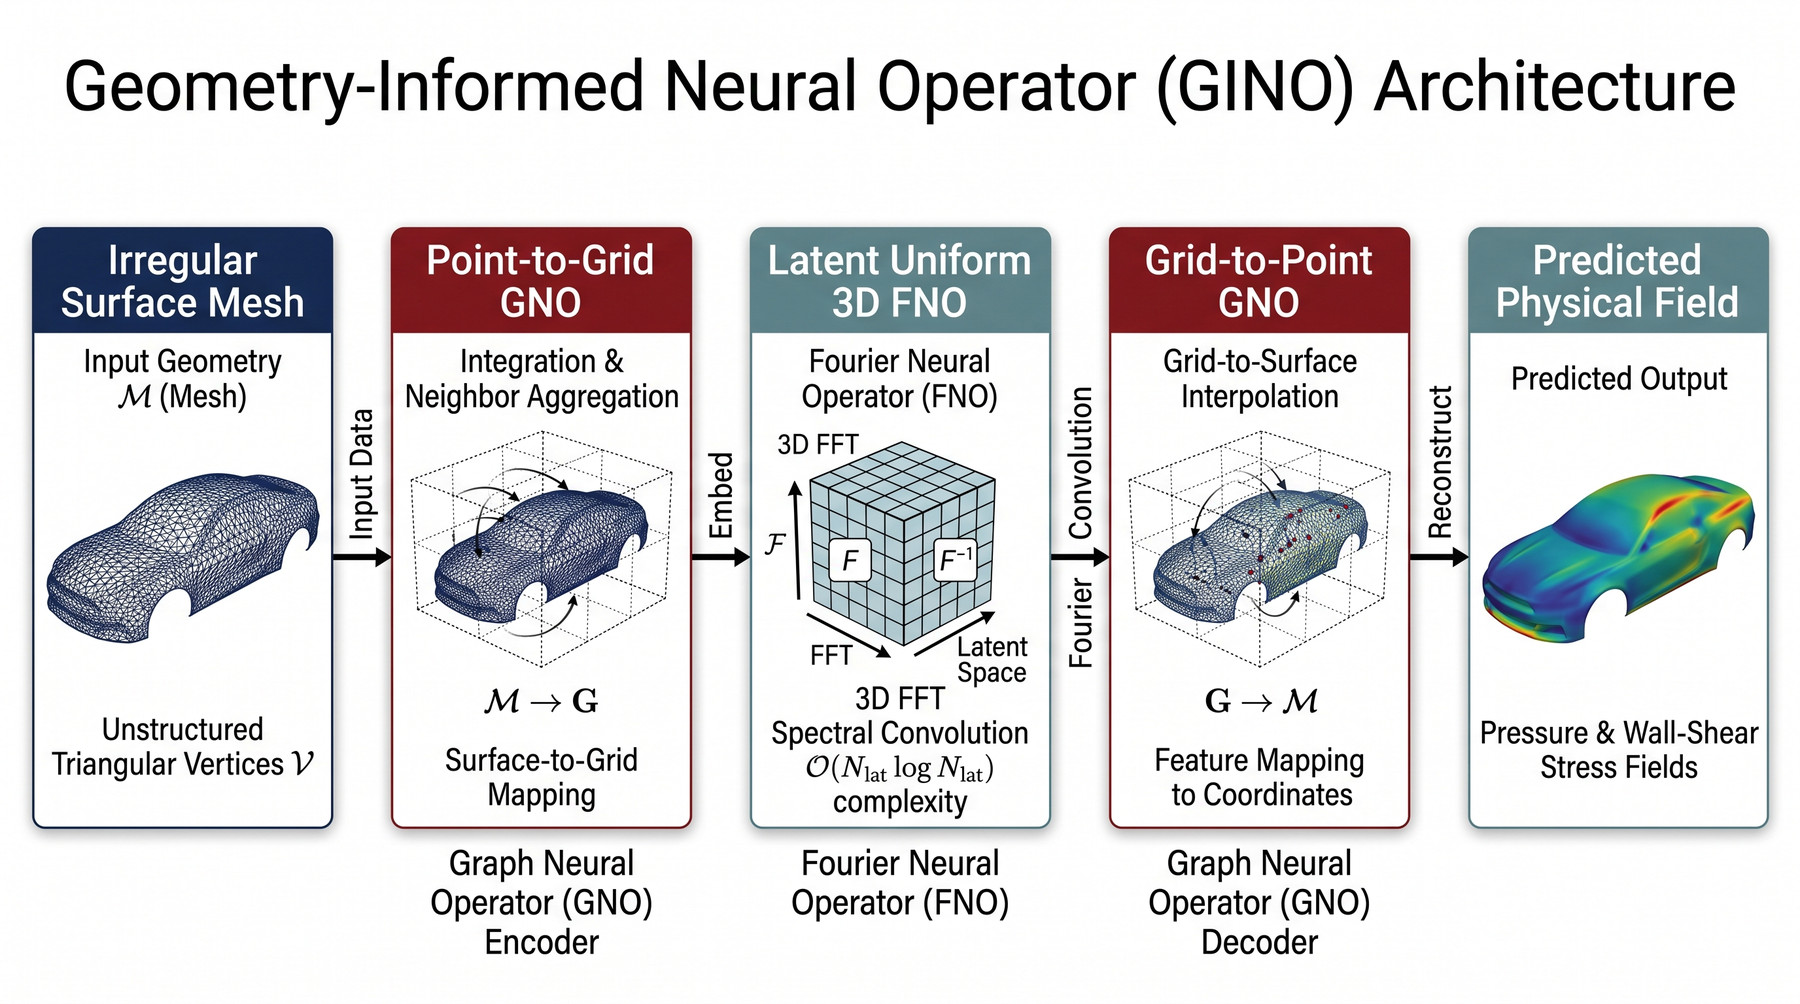
\includegraphics[width=0.92\textwidth]{fig_gino_pipeline.jpg}
\caption{\textbf{The Geometry-Informed Neural Operator (GINO) workflow.} An irregular surface mesh $\mathcal{M}_{\text{surf}}$ is projected onto a regular 3D latent bounding grid via a Point-to-Grid GNO layer. A fast 3D FNO processes latent features with $\mathcal{O}(N_{\text{lat}} \log N_{\text{lat}})$ spectral efficiency. Finally, a Grid-to-Point GNO decoder projects the processed latent state back to arbitrary surface evaluation coordinates.}
\label{fig:gino}
\end{figure}

The end-to-end pipeline operates in three distinct stages, and they are best described as one
quadrature, one transform stack, and the same quadrature run backwards. The
\textbf{point-to-grid encoder} integrates surface features $v_{\text{surf}}(x)$ onto a
regular, uniform latent grid $\Omega_{\text{latent}} \subset
\mathbb{R}^{H \times W \times D}$,
\index{point-to-grid projection}\index{Geometry-Informed Neural Operator (GINO)!pipeline stages}
\begin{equation}
  \label{eq:ch24-p2g}
  v_{\text{grid}}(z_k) = \sum_{x_j \in \mathcal{M}_{\text{surf}}} \kappa_{\text{enc}}(z_k - x_j)
  \, v_{\text{surf}}(x_j) \, w_j,
\end{equation}
where $z_k$ ranges over latent grid nodes and $w_j$ is again the tributary area of the surface
vertex $x_j$. Equation \eqref{eq:ch24-p2g} is \eqref{eq:ch24-gno-kernel} with the roles of
source and target interchanged, and the same sparsification choice: evaluated for every pair
$(z_k, x_j)$ the encoder costs $\Theta(N_{\text{lat}} N_{\text{surf}})$, which is precisely
the dense interaction \chapref{ch:part1-comparative-theoretical-taxonomy-of-archit} flags
beside \eqref{eq:ch8-gino}, so a workable implementation restricts the sum to surface points
within a radius of $z_k$ and recovers the edge-linear count. The
\textbf{latent operator processing} then applies stacked 3D Fourier neural operator layers to
$v_{\text{grid}}$; the structured layout is exactly $(B, C, H, W, D)$, and the layer is the
two-dimensional \texttt{SpectralConv2d} of
\chapref{ch:part2-fourier-neural-operators-fno-from-scratch} with one axis added --- a
real-input transform over three spatial axes in place of \texttt{rfft2}, the two-dimensional
real fast Fourier transform (FFT), a mode box that is a product of three contiguous index
ranges, \eqref{eq:ch05-modeset} read at $d=3$ rather than the planar $d=2$, and a contraction
written in
\texttt{einsum} notation (Einstein summation)\index{einsum contraction} with one index more.
Global communication in $\mathcal{O}(N_{\text{lat}} \log N_{\text{lat}})$ operations is what
that stage buys, and it is what the radius-$r$ layers cannot buy cheaply. The
\textbf{grid-to-point decoder} closes the pipeline by sampling the latent grid at the surface
evaluation coordinates,
\begin{equation}
  \label{eq:ch24-g2p}
  v_{\text{surf}}(x_i) = \sum_{z_k \in \mathcal{N}_r(x_i)} \kappa_{\text{dec}}(x_i - z_k) \,
  v_{\text{grid}}(z_k) \, \tilde{w}_k,
\end{equation}
which is \eqref{eq:ch24-p2g} read in the other direction: $\tilde{w}_k$ is now the cell volume
of the latent node rather than a surface dual area, and the output is indexed by the mesh, not
by the box. Because the evaluation points in \eqref{eq:ch24-g2p} are free arguments of the
decoder, the same trained weights return pressure and WSS on a tessellation that was never in
the training set --- the property that makes the construction a surrogate for a design sweep
rather than a predictor for a single part \cite{li2023geometry}.

Two further inputs carry geometry that the connectivity alone does not supply, and the two
layouts take them differently. On the mesh, the coordinates stay in the index structure rather
than becoming channels, exactly as \chapref{ch:part2-the-practitioner-s-paradigm-infinite-dimen}
found: they enter \eqref{eq:ch24-gno-kernel} as the displacement argument $x_i - x_j$, which is
how the \texttt{coords} tensor enters Listing~\ref{lst:gno-kernel-conv}. On the latent grid the
geometry has to become channels, and the field that does it is the signed distance function
(SDF) --- the distance from any point to the body's surface, negative inside
\index{signed distance function (SDF)}--- concatenated with the grid's own coordinates, so the
spectral operator can tell a solid from a void rather than inferring it from a sparse shell of
projected features. Without such an encoding, the interior of the bounding box is
indistinguishable from empty space and the burden of the geometry falls entirely on the two
graph interfaces.

Batching is where irregular geometry costs real engineering time. The structured layout of
\chapref{ch:part2-the-practitioner-s-paradigm-infinite-dimen}, $X \in
\mathbb{R}^{B \times C \times N_1 \times \cdots \times N_d}$, presumes that every sample
shares its shape, and the point-cloud layout $X_{\text{nodes}} \in
\mathbb{R}^{B \times N_{\text{nodes}} \times C}$ presumes that every mesh has the same node
count --- false the moment two bodies are compared.
\index{batching!irregular geometries}\index{point-cloud layout!ragged batches}Padding to the
largest mesh and masking the surplus edges works, but it converts raggedness into wasted
compute rather than removing it; per-sample loops with accumulated gradients keep memory
predictable and forfeit throughput; bucketing by node count splits the batch and complicates
the sampler. This is why the forward signature in Listing~\ref{lst:gno-kernel-conv} carries no
batch axis at all: it is one mesh per call. The GINO composition softens the problem rather
than solving it --- the ragged structure is confined to the encoder and decoder, while the
latent grid inside has a fixed shape that batches cleanly, which is a genuine advantage of
placing the expensive operator on a box.

% -----------------------------------------------------------------------------
\section{What Irregular Geometry Buys, and What It Costs}
\label{sec:ch24-ledger}
% -----------------------------------------------------------------------------

The comparison borrows three of the five axes
\chapref{ch:part1-comparative-theoretical-taxonomy-of-archit} fixes --- which class of kernels a
parameterization admits, what one query costs at a chosen resolution, and how strong a theorem
is attached to the class --- and leaves its other two, inductive bias and the relation between
parameter space and discretization, to the memory accounting and the refinement behavior below.
Against the FNO, on the first axis a graph layer keeps the kernel's
dependence on $a(x_i)$ and $a(x_j)$ and its support constraint in place of stationarity and
band-limiting, and it drops the requirement that the domain be a torus
\cite{kovachki2023neural,li2021fourier}. On the second axis it pays more: $\Theta(|E|\,
d_v^{2})$ per layer, quadratic in channel width on \emph{every} edge, against $\Theta(d_v N
\log N + K d_v^{2})$ for a spectral layer, where the quadratic term is confined to the $K$
retained modes. GINO's hybrid pays $\Theta(|E| + N_{\text{lat}} \log N_{\text{lat}})$ --- edge
work only at the interfaces --- but the latent box is a design parameter with a real floor:
$N_{\text{lat}} = HWD$ covers the bounding volume, so a slender body in a large box spends
most of its spectral budget on empty space, and the resolution needed to capture a thin
boundary layer sets the cost of the whole box. GNO and GINO
\index{Graph Neural Operator (GNO)!cost versus spectral layer}\index{Geometry-Informed Neural Operator (GINO)!cost of the latent box}
also differ from the FNO in what refinement touches. For the spectral operator the parameters
are mesh-free and one trained $\theta$ is queried at any $N$; for a graph operator the
parameters are mesh-free too, but the \emph{graph} is an input, so refinement changes $|E|$,
the memory footprint, and the realization of the layer rather than leaving $\theta$ alone
against a new grid. The third axis is the one on which honesty is cheapest: Part~I's ledger
Table~\ref{tab:ch8-ledger} records no universality statement, no rate, and no invariance proof
for either architecture, and the reason is visible in \eqref{eq:ch24-gno-kernel} --- a
radius-$r$ ball is a truncation of the kernel's support whose error is controlled by whatever
regularity the target has in the pair $(x,y)$, a question no theorem in this book answers.

What the geometry buys is scope rather than accuracy. It lets one trained operator serve a
parameterized family of bodies whose meshes differ in node count, connectivity, and spacing; it
lets the output be sampled wherever the engineer wants it rather than where the grid happens
to put nodes; and it retains the input-dependent kernel that inhomogeneous problems ask for.
The aerodynamic application, with its reported accuracy and its inference budget against a
volume solver, is taken up with the other large-scale 3D workloads in
\chapref{ch:part3-external-aerodynamics-and-surface-flows}. What it costs is edge-linear
computation with a quadratic channel factor, a memory footprint that scales with mesh size
rather than with parameters, an SDF and coordinate-channel pipeline that must be rebuilt for
every new computer-aided design tessellation, ragged batching at the two
interfaces, and the loss of every guarantee the spectral case enjoys.

One further obligation is procedural rather than architectural. The error split of
\eqref{eq:ch01-error-split} presupposed a discretization that was a refinement of one fixed
grid; here the graph is itself an argument of the layer. A reported error for a graph
surrogate is therefore a triple --- model, mesh, and metric --- and the protocol that makes it
readable evaluates the trained operator on the training tessellation, then on a
re-tessellation of the same body at different node density, and against a solver run on the
evaluation mesh rather than on the one the data came from. Where those three numbers diverge,
the divergence localizes in the quadrature of \eqref{eq:ch24-gno-kernel} --- in the weights,
the radius, or the depth needed to span the body --- a term the spectral construction can
leave implicit and this one cannot.

\takeaway{Graph Layers Are a Support Constraint, Not a New Family}{A GNO layer is the generic integral-kernel layer \eqref{eq:no_layer} with the kernel's support restricted to a radius-$r$ neighborhood and the mesh entering only through quadrature weights, so parameters stay mesh-free while the sum tracks the continuum integral. GINO confines that machinery to a point-to-grid encoder and a grid-to-point decoder and runs the global part of the operator on a latent grid, where a fast Fourier transform is legal and the mixing needs no depth to reach across the body. Neither construction restores a convergence guarantee.}

% -----------------------------------------------------------------------------

The three canonical problems that follow are chosen for the opposite reason. Burgers'
equation, Darcy flow, and the two-dimensional Navier--Stokes equations are posed on the
periodic torus or the unit square precisely so that a discrete Fourier transform is legal,
which makes them the controlled setting in which the spectral machinery of
\chapref{ch:part2-fourier-neural-operators-fno-from-scratch} can be judged without geometry in
the way \cite{li2021fourier}. \chapref{ch:part2-canonical-pde-benchmarks-and-reference-wor}
assembles those reference workflows: the input measures, the resolutions at which training and
evaluation grids differ, the relative-$L^{2}$ metric of
\chapref{ch:part2-the-practitioner-s-paradigm-infinite-dimen} that all three chapters share,
and the convergence behavior a practitioner should expect before tuning anything. Two of this
chapter's obligations carry forward there. The first is bookkeeping: an error number for a
graph operator must state the mesh it was measured on, since the mesh is part of the input
rather than an accident of the discretization. The second is methodological: the benchmarks
are where a reader can establish, on problems with a known answer, what the quadrature weights
and radius choices of \eqref{eq:ch24-gno-kernel} are supposed to accomplish before paying for
a latent box and a tessellated surface.

% Chapter 14: Canonical PDE Benchmarks and Reference Workflows
% Part II of the book.

\chapter{Canonical PDE Benchmarks and Reference Workflows}
\label{ch:part2-canonical-pde-benchmarks-and-reference-wor}
\label{sec:benchmarks}
% -----------------------------------------------------------------------------

Every architecture in Part~II has now been written down, and none has been
measured. This chapter supplies the missing half of the contract: the problems on
which \chapref{ch:part2-deeponet-engineering-branch-trunk-networks} through
\chapref{ch:part2-graph-neural-operators-gno-and-irregular-g} are trained, and
the protocol that makes a reported error interpretable. The difficulty is not a
shortage of test cases but the looseness with which they are described. A partial
differential equation (PDE) is not a benchmark. A benchmark is the equation
together with seven further objects: its nondimensional parameters, its domain
and boundary conditions, a probability measure on the input functions, the
classical solver that generated the paired data, the partition of that data into
training, validation, and test sets together with any normalization applied to
it, the error metric and the order in which it is averaged, and the
resolution-transfer protocol on which mesh independence is either demonstrated or
quietly dropped. Fix six of the seven and the seventh becomes a license to report
whatever number is convenient.

Part~I makes the stakes precise.
Theorem~\ref{thm:fno_convergence} bounds a truncation term and a neural
parametric term for operators that gain $\alpha$ derivatives;
\eqref{eq:ch01-error-split} adds discretization and statistical terms to that
account; and \chapref{ch:part1-open-theoretical-problems-and-mathematical} argues
that the relative $L^{2}$ metric forgives precisely the defects a shock leaves
behind. Every one of those statements is about a space, a measure, and a norm, so
none can be checked against a number whose protocol is unstated. The three
problems below are ordered by which term of that decomposition they load, and
Section~\ref{sec:ch25-protocol} says what each one tests and where its measured
behavior stops.

The reader should bring PyTorch \cite{paszke2019pytorch} and its vocabulary: a
graphics processing unit (GPU) tensor, a batch dimension, a forward pass. The fast
Fourier transform (FFT) and the layout conventions of
\chapref{ch:part2-the-practitioner-s-paradigm-infinite-dimen} are prerequisites in
the concrete sense that every shape and operation count below is inherited from
them. The first section fixes the reporting protocol and names the axis along
which the three benchmarks differ; the remaining three give each problem its
specification, its tensor shapes, its failure behavior, and its measured accuracy
where accuracy has been measured. The material is assembled with
Appendix~\ref{app:c} in view, whose benchmark sheets are meant to be transcribed
from here. Figure~\ref{fig:benchmarks} carries the chapter's one computed plot: the
Burgers target family the first benchmark must reproduce, obtained from the exact
Cole-Hopf solution rather than from a run. Everything else here is arithmetic or a
citation, and is to be read as such. No Darcy accuracy curve is presented, because
no such curve was measured for this book; the Darcy figures that appear below are
stated values, and Appendix~\ref{app:c} records them as such.

\begin{figure}[t]
\centering
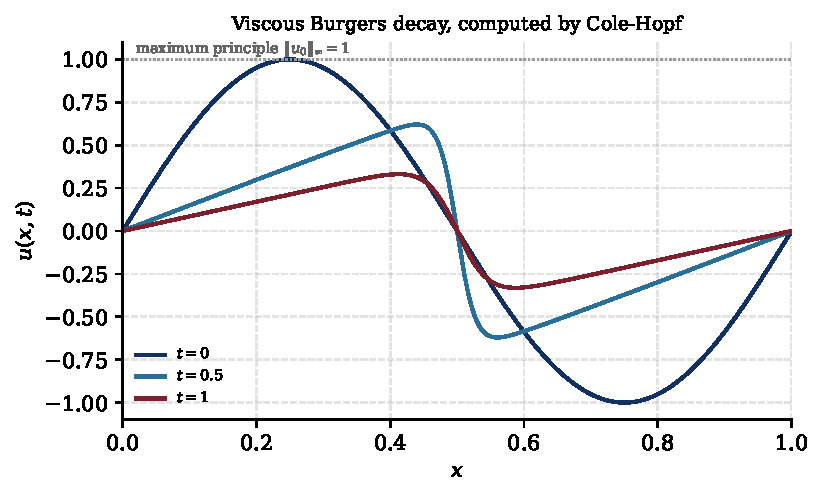
\includegraphics[width=0.80\textwidth]{fig_burgers_exact.pdf}
\caption{\textbf{The Burgers target family, computed exactly.} Viscous Burgers' equation $u_t + u u_x = \nu u_{xx}$ on $[0,1)$ periodic with $\nu = 0.01$ and $u_0(x) = \sin(2\pi x)$, solved by the Cole-Hopf substitution $u = -2\nu\,\partial_x \log \phi$ with $\phi_t = \nu \phi_{xx}$ and $\phi(x,0) = \exp[\cos(2\pi x)/(4\pi\nu)]$. Every trace is computed from the exact solution: the peak falls from $1$ at $t = 0$ to $0.6207$ at $t = 0.5$ and $0.3312$ at $t = 1$, and the profile stays under the maximum-principle bound $\|u_0\|_{\infty} = 1$, drawn as the dotted line. The steepening front near $x \approx 0.5$ is the feature the benchmark scores. Produced by \texttt{figures/make\_figures.py}, which asserts the initial condition, a relative PDE residual and grid independence before writing the file.}
\label{fig:benchmarks}
\end{figure}

% -----------------------------------------------------------------------------
\section{Reference Workflows: What a Benchmark Specification Must Contain}
\label{sec:ch25-protocol}
% -----------------------------------------------------------------------------

Begin with the metric, because it is where the book's two halves meet. All three
benchmarks are scored with the relative $L^{2}$ error
\eqref{eq:rel_l2_loss} of
\chapref{ch:part2-the-practitioner-s-paradigm-infinite-dimen}, the discretized
form of the population risk \eqref{eq:ch01-risk}: the $L^{2}(\Omega)$ norm of the
error divided by the $L^{2}(\Omega)$ norm of the reference field, computed per
sample and then averaged over the batch. The order of those two operations is a
specification choice, not a notational one. A mean of per-sample relative errors
weights a low-amplitude sample as heavily as a high-amplitude one, whereas the
ratio of aggregated norms is dominated by the largest fields in the batch; on a
measure whose amplitude varies by an order of magnitude the two summaries can
differ by a factor of two, and a paper that reports ``relative $L^{2}$ error''
without saying which it used has reported an unidentifiable quantity. Where the
gradient of the field matters more than its energy, as it does for the shock
snapshots below, the honest choice is the inhomogeneous $H^{1}$ functional
\eqref{eq:ch07-sobolev-loss}, which the loss module of
Listing~\ref{lst:ch21-lploss} evaluates once its caller supplies differentiated
fields: one extra differentiation of prediction \emph{and} label, bought for control
of the quantity most applications read.
\index{relative $L^{2}$ error!as benchmark metric}
\index{error metric!per-sample versus batch-aggregated}

Next comes the paired data, and here the arithmetic of amortization from
\eqref{eq:ch01-cost-bookkeeping} becomes concrete. The reference solutions are
produced by classical solvers whose per-query costs are tabulated in
Table~\ref{tab:benchmarks_hardware}: roughly $1.5$ seconds for a finite element
method (FEM) Darcy solve, $4.8$ seconds for a pseudo-spectral Navier--Stokes
trajectory. A thousand training pairs therefore cost about twenty-five minutes of
wall-clock FEM work and eighty minutes of time integration---cheap by simulation
standards, which is why these three problems remain the field's defaults even
though only the Darcy problem arrives in a form an application uses unchanged. The
cost is also a constraint on
honesty: the discretization term in \eqref{eq:ch01-error-split} is invisible if
the reference solver's own resolution is not comfortably finer than the grid on
which the surrogate is trained, since the network is then fitting a solution that
the solver never computed. Record the solver, its spatial and temporal
discretization, its nonlinear and linear tolerances, and the grid on which the
reference was sampled, and sample the reference at least as finely as the finest
evaluation grid the surrogate will see.
\index{pseudo-spectral method!as reference solver}
\index{data generation!reference solver tolerances}

The remaining items of the protocol are short to state and routinely omitted. The
input measure must be given as a measure, not as one representative draw; the
normalization of
\chapref{ch:part2-the-practitioner-s-paradigm-infinite-dimen}---pointwise mean and
standard deviation fields computed over the training ensemble only---must be
frozen before validation data are touched, because normalizing with test
statistics leaks information and inflates accuracy by an amount that grows as the
test set shrinks; and the train/validation/test partition must be reported, an
obligation this chapter discharges by noting that no split ratio is recorded in
what follows, so none of the numbers below should be read as a leaderboard entry.
A single convention worth naming, though none of the numbers below tests it, is
mode-count augmentation: randomly truncating
the retained band below the training maximum should make one checkpoint usable across
several mode budgets, at the price of a slightly worse error at the full budget.
\index{input measure!reporting requirement}
\index{data normalization!frozen before validation}
\index{data augmentation!mode truncation}

Resolution transfer is the protocol item that separates an operator from a
network with a fixed input size, and Part~I states exactly when it is free.
Proposition~\ref{prop:ch06-zeroshot} proves that the spectral branch of a
truncated Fourier neural operator (FNO) returns the identical continuous output,
before the activation, on any grid finer than
$N_{\text{train}} > 2k_{\max}$, provided the input is band-limited within the
retained set $Z_{k_{\max}}$ of \eqref{eq:ch05-modeset}. The hypothesis is the
caveat. None of the three benchmarks below satisfies it: the Burgers target
acquires a shock, the Darcy coefficient field is a rough random function, and the
Navier--Stokes vorticity has a broad spectrum by construction. Super-resolution
results on these problems are therefore measurements, not corollaries, and must be
reported as errors at $N_{\text{test}}$ alongside errors at $N_{\text{train}}$.
\index{resolution transfer!evaluation protocol}
\index{band-limited input!failure on benchmark data}

What, then, distinguishes the three problems? Not size, and not difficulty, but
the term of \eqref{eq:ch05-error-decomposition} each one loads. Darcy flow is an
elliptic coefficient-to-state map that gains derivatives, so its truncation term
decays algebraically in $k_{\max}$ and the theorem applies with its hypotheses
nearly satisfied. Burgers' equation is a parabolic evolution map that also gains
derivatives at fixed $\nu > 0$, but with a constant that deteriorates as the
viscous layer narrows, so the same bound becomes vacuous precisely where the
problem becomes interesting. Navier--Stokes is trained as a one-step map, whereas
applications consume its $K$-fold composition, and the quantity that matters is
the rollout bound \eqref{eq:ch09-gronwall}, whose amplification factor
$\Lambda_{\theta}$ no approximation theorem in this book controls. Three
benchmarks, three different failure modes of one inequality. Figure~\ref{fig:benchmarks}
documents the first two; the third, specified in
Section~\ref{sec:ch25-navierstokes}, comes with no accuracy claim attached,
because none was measured.
\index{benchmark!specification checklist}
\index{benchmark taxonomy}

% -----------------------------------------------------------------------------
\section{Benchmark 1: 1D Viscous Burgers' Equation}
\label{sec:ch25-burgers}
% -----------------------------------------------------------------------------

The 1D viscous Burgers' equation is governed by
\begin{equation}
  \label{eq:ch25-burgers}
  \partial_t u + u \partial_x u = \nu \partial_{xx} u, \qquad x \in [0, 1), \quad t \in [0, 1],
\end{equation}
with periodic boundary conditions. The domain is therefore the torus
$\mathbb{T} = \mathbb{R}/\mathbb{Z}$, not an interval: periodicity is what licenses
the Fourier representation, and it also removes any boundary condition from the
specification, which is why \eqref{eq:ch25-burgers} is the cleanest of the three
tests of discretization invariance. The state is scalar, so the physical input and
output channel counts are both one; the datum is the initial condition $u_0$, and
the target is $u(\cdot, t)$ at one or more times in $[0,1]$. This is a
forward time-evolution operator of the kind introduced in
\eqref{eq:ch03-burgers}, with domain and codomain the same space, in contrast to
the coefficient-to-state map of Section~\ref{sec:ch25-darcy}.

The viscosity is the whole specification. Panel~(a) of Figure~\ref{fig:benchmarks}
is drawn at $\nu = 0.01$, a tenth of the $\nu = 0.1$ of the cited Burgers
experiment \cite{li2021fourier}; its initial trace is consistent with
$u_0(x) = \sin(2\pi x)$, amplitude one. Part~I computes the inviscid gradient
catastrophe for exactly that family: $t_{*} = (2\pi A)^{-1}$, which at $A = 1$ is
$t_{*} \approx 0.16$, occurring where the initial slope is most negative, at
$x = 0.5$. Both snapshots in the panel, $t = 0.5$ and $t = 1.0$, lie well past
that time, so what the reader sees is not steepening in progress but a settled
viscous shock: the $t = 0.5$ trace has developed a sharp descent through zero at
$x \approx 0.5$, and by $t = 1.0$ the descent is confined to a narrow layer with
the smooth remainder of the wave barely changed. The panel is a schematic of the
target family rather than a predicted field, and one feature of it is worth using
as a check on any solver or surrogate. At $\nu > 0$ the maximum principle for
\eqref{eq:ch25-burgers} gives $\sup_x u(\cdot, t) \le \sup_x u_0 = 1$ for all $t$,
yet the $t = 1.0$ trace crests marginally above the initial maximum. A computed
profile that exceeds $\|u_0\|_{L^{\infty}}$ has produced an artifact---an
under-resolved layer, or the ringing of a trigonometric representation near a steep
front---not a feature, and no relative $L^{2}$ number will tell you so.
\index{Burgers equation!benchmark specification}
\index{shock wave!viscous layer width on a grid}
\index{maximum principle!as an implementation check}

Resolution is set by the same layer width. The compressive shock connecting states
$u^{-} > u^{+}$ has the profile \eqref{eq:ch03-shockprofile}, whose transition
layer measures $4\nu/(u^{-} - u^{+})$; writing $\ell_{\nu}$ for that width, at
$\nu = 0.01$ and an order-unity jump $\ell_{\nu} \approx 0.04$ in units of $x$. On
$N = 128$ cells ($\Delta x \approx 7.8 \times 10^{-3}$) the layer spans about five
cells, which is enough for a grid function to represent its shape; on $N = 64$ it
spans two and a
half, which locates the front but no longer resolves the profile, so what the grid
holds is an alias of a shock rather than a shock. That arithmetic, not
a preference for large grids, is why $N = 128$ is the coarsest defensible choice for
this benchmark; it is not the grid of the errors quoted below, which are reported
at $s = 256$ to $s = 8192$ \cite{li2021fourier}. It
also explains the tension Part~I records between accuracy and discontinuity: the
spectral branch represents nothing outside $Z_{k_{\max}}$, so a shock's
$|\hat{u}(k)| = O(|k|^{-1})$ tail is truncated by hypothesis, and the truncation
term of \eqref{eq:ch05-error-decomposition} carries a constant that grows as
$\nu \to 0$.

Tensors and cost follow the layout of
\chapref{ch:part2-the-practitioner-s-paradigm-infinite-dimen}. A batch of initial
conditions arrives as $(B, 1, 128)$; one normalized coordinate channel is
appended---one rather than two, this being a one-dimensional geometry---giving
$(B, 2, 128)$; lifting to width $d_v$ and taking the real FFT along the last axis
gives $(B, d_v, 128, 65)$ complex, of which the two retained blocks at either end
of the spectrum, $(B, d_v, m)$ each, are multiplied by the learned weights. Here $m$
is the retained mode count per band edge---written $m_x, m_y$ in the
two-dimensional tally below, and not to be confused with the $100$ sensor readings of
the DeepONet baseline in Figure~\ref{fig:benchmarks}(b), which the legend also labels
$m$. With
$m = 12$ and $d_v = 32$ the two complex weight tensors hold
$4 m d_v^{2} \approx 4.9 \times 10^{4}$ real numbers per layer, against a
transform cost $\mathcal{O}(d_v N \log N)$ that is essentially flat in $m$: the
one-dimensional benchmark is parameter-cheap and resolution-cheap, which is what
makes it the natural first experiment after Appendix~\ref{app:b}'s heat equation.
\index{tensor layout!benchmark batch shapes}

The number
\chapref{ch:part1-open-theoretical-problems-and-mathematical} interrogates is the
cited paper's own; the book never measured it. The source fixes the
viscosity at $\nu = 0.1$ (Appendix A.3.1) and learns
$u_{0} \mapsto u(\cdot, 1)$, the solution at time one---one output time only
(Section 5.1). Its Table 3 lists relative $L^{2}$ errors
$0.0149$, $0.0158$, $0.0160$, $0.0146$, $0.0142$, $0.0139$ at evaluation
resolutions $s = 256, 512, 1024, 2048, 4096, 8192$; two of the six exceed
$1.5\%$, and no $128$-point Burgers grid appears anywhere in that paper: the
$N = 128$ of the preceding paragraph is this book's own choice, and the two
configurations are distinct. Three qualifications belong to that row, and a
snapshot family would need its own. First, the ambiguity is this book's, not the
source's: the
cited operator ends at $t = 1$, while this section targets $u(\cdot, t)$ at one
or more times, so the reader must still ask whether one model is trained per
$t$, or one model consumes $t$ as an extra input channel, or a one-step map is
iterated to reach $t$; these are three different operators, and the paper does
not say which was trained. Second, each entry of the quoted row compares two
grid functions at the same $s$, the reference subsampled from an $8192$-point
solve (Appendix A.3.1), so it
conflates the approximation and discretization terms of
\eqref{eq:ch01-error-split}. Third, and decisively, the metric is the forgiving
one: as \chapref{ch:part1-open-theoretical-problems-and-mathematical} shows, a
Gibbs overshoot of fixed height on a set of measure $O(1/M)$ contributes
$O(M^{-1/2})$ and a displacement $\delta$ of a unit-height front contributes
$\sqrt{2\delta}$, so a score of $1.4\%$ to $1.6\%$ is fully compatible with a shock placed
in the wrong cell. The benchmark remains the right test---it is the only one of
the three whose target loses regularity---but it should be reported with an
$H^{1}$ or a front-location error beside the $L^{2}$ number.
\index{Burgers equation!snapshot operator ambiguity}

% -----------------------------------------------------------------------------
\section{Benchmark 2: 2D Steady-State Darcy Flow}
\label{sec:ch25-darcy}
% -----------------------------------------------------------------------------

The Darcy flow problem tests an operator's ability to map heterogeneous
coefficient fields to smooth potential solutions:
\begin{equation}
  \label{eq:ch25-darcy}
  -\nabla \cdot \big( K(x) \nabla u(x) \big) = f(x), \qquad x \in [0, 1]^2, \quad u|_{\partial\Omega} = 0.
\end{equation}
Two differences from \eqref{eq:ch25-burgers} matter more than the change of
dimension. The map here is coefficient-to-state: the input is $K$, the output is
$u$, and the spaces differ, so the operator is smoothing rather than
evolutionary---it is the benchmark form of \eqref{eq:darcy}, with the roles of
$a$ and $K$ identified. And the boundary condition is homogeneous Dirichlet on a
square, not periodicity on a torus, which is inconvenient for a spectral
architecture: the Fourier machinery of
\chapref{ch:part2-fourier-neural-operators-fno-from-scratch} is exactly a
representation on $\mathbb{T}^2$, so either the domain is treated as periodic and
the mismatch with $u|_{\partial\Omega} = 0$ is absorbed into the learned map, or
the field is odd-extended. A specification that does not say which has been done
leaves the dominant error term unnamed.

The log-permeability is drawn from a Gaussian random field (GRF), which makes $K$
itself log-normal,
\begin{equation}
  \label{eq:ch25-darcy-measure}
  \log K \sim \mathcal{N}\big(0, (-\Delta + \tau^{2} I)^{-d}\big), \qquad d = 2,
\end{equation}
with $\tau$ a correlation-length parameter and $-\Delta$ the Laplacian with the
problem's own boundary condition \cite{stuart2010inverse}---a Mat\'ern-type
covariance, the standard prior for subsurface coefficients. Read as a covariance
operator, \eqref{eq:ch25-darcy-measure} assigns the mode $k$ a variance of order
$(1 + |k|^{2})^{-2}$, so the sum $\sum_{k} |k|^{2s}(1+|k|^{2})^{-2}$ converges
exactly when $s < 1$ in two dimensions: sample paths of $\log K$ lie in
$H^{s}$ for $s < 1$ and in no better space. Since continuity in two dimensions
requires $s > d/2 = 1$, the coefficient is almost surely unbounded, $K$ is
log-normal rather than essentially bounded, and Assumption~\ref{ass:ellipticity}
fails on the support of the raw measure. This is not a pathology to be tolerated
but a specification to be repaired: draws are truncated into a band
$K \in [K_{\min}, K_{\max}]$ before use, and the band is part of the benchmark,
because the elliptic estimate Part~I derives for \eqref{eq:darcy} is uniform only
over coefficient sets bounded away from zero and from above. Report $K_{\min}$ and
$K_{\max}$ as carefully as the error.
\index{Gaussian random field!Matern-type covariance}
\index{log-normal permeability!truncation and ellipticity}
\index{Darcy flow!benchmark specification}

The regularity that survives is enough to make the benchmark theoretically clean.
With $K$ bounded and measurable, the energy estimate gives $u \in
H^{1}_{0}(\Omega)$; with $K$ smooth, classical regularity lifts the solution to
$H^{2}(\Omega)$. The solution operator therefore has a positive smoothing order
$\alpha$ in the sense of Theorem~\ref{thm:fno_convergence}, its image of a bounded
input set is precompact in $L^{2}$ by Rellich--Kondrachov, and the truncation term
$C_1 k_{\max}^{-\alpha}$ is a live prediction rather than a formality. That is why
\eqref{eq:ch25-darcy} is the default test of the approximation theory and the
default data source for porous-media work \cite{li2021fourier, wen2022ufno}.

Tensor shapes are the two-dimensional case of the tally in
Section~\ref{sec:ch25-burgers}, and larger by the square: a batch arrives as
$(B, 1, 64, 64)$, two coordinate channels make it $(B, 3, 64, 64)$, lifting gives
$(B, d_v, 64, 64)$, and \texttt{torch.fft.rfft2}---the real-to-complex transform
along the two trailing axes---returns $(B, d_v, 64, 33)$ complex, the half-spectrum
being all that conjugate symmetry requires. The two retained corners at
$m_x = m_y = 12$ hold $4 m_x m_y d_v^{2} \approx 5.9 \times 10^{5}$ real numbers
per layer at $d_v = 32$, so four layers carry roughly $2.4$ million spectral
parameters, which is the budget the error floor below buys. The \texttt{einsum}
contracting channels mode by mode is the second term of \eqref{eq:ch8-costs},
$\mathcal{O}(|Z_{k_{\max}}| d_v^{2})$ per
layer, and does not grow with the grid at all; only the transforms do, near-linearly.

No accuracy comparison in this chapter is measured
here; the one it reports is transcribed from the paper that introduced the
benchmark. Table 4 of \cite{li2021fourier} scores the 2-d Darcy problem at four
evaluation resolutions, and FNO returns $0.0108$, $0.0109$, $0.0109$, $0.0098$ at
$s = 85, 141, 211, 421$, against $0.0332$--$0.0369$ for the graph neural operator,
$0.0244$--$0.0259$ for the reduced-basis method and $0.1716$ for a feed-forward
network. Two features of that ordering are architectural rather than matters of
tuning. A convolutional stack aggregates over a receptive field that grows only
with depth, while the pressure at a point of \eqref{eq:ch25-darcy} responds to the
coefficient everywhere --- the long-range coupling Part~I attributes to the Green
kernel --- so its accuracy is limited by distance, not capacity; the fully
convolutional row is the one entry whose error rises monotonically with
resolution, from $0.0253$ to $0.1097$. The FNO's global spectral branch removes the
distance limitation, and its error is essentially flat across the four grids, which
is the resolution-invariance claim of \chapref{ch:part1-discretization-invariance-and-continuum-li}
showing up as an accuracy column rather than as a theorem. What the table does not
settle is the cost of reaching that error: it reports held-out accuracy at four
resolutions and nothing about epochs, hardware or training time, and no
epoch-by-epoch curve for any of these architectures is reproduced in this book.
Multi-scale variants that interleave residual blocks with spectral convolution are
reported to improve precisely this regime on sharper multiphase problems
\cite{wen2022ufno}.
\index{U-Net!as benchmark baseline}
\index{DeepONet!as benchmark baseline}
\index{validation curve!plateau versus divergence}

% -----------------------------------------------------------------------------
\section{Benchmark 3: 2D Incompressible Navier-Stokes Equations}
\label{sec:ch25-navierstokes}
% -----------------------------------------------------------------------------

The 2D incompressible Navier--Stokes equations in vorticity formulation are
\begin{equation}
  \label{eq:ch25-navierstokes}
  \partial_t \omega + \mathbf{u} \cdot \nabla \omega = \nu \Delta \omega + f, \qquad \nabla \cdot \mathbf{u} = 0, \quad \omega = \nabla \times \mathbf{u},
\end{equation}
on the doubly periodic torus $\mathbb{T}^{2} = [0,1)^{2}$. In two dimensions
$\omega$ is the scalar $\partial_1 u_2 - \partial_2 u_1$, and the divergence-free
velocity is recovered from it by the Biot--Savart law
$\mathbf{u} = \nabla^{\perp}(-\Delta_{\mathbb{T}^2})^{-1}\omega$ of
\chapref{ch:part1-partial-differential-equations-as-solution}, so
\eqref{eq:ch25-navierstokes} is a closed equation for one scalar field with no
pressure to eliminate. Periodicity replaces the no-slip condition of a wall-bounded
flow; that single choice is what makes the pseudo-spectral reference solver cheap
and the benchmark standard, and it is also what limits its transfer to
applications, where boundary layers carry the drag. The tensor bookkeeping differs
from Section~\ref{sec:ch25-darcy} in one respect worth stating: the forcing is
fixed and time-independent, so it carries no information across the ensemble and
needs no input channel, and a state enters as $(B, 1, N, N)$ with a single channel
in and out. What the ensemble varies is the initial vorticity---and the viscosity,
if more than one is trained at once, which the paragraph below argues against.

The forcing is Kolmogorov's,
\begin{equation}
  \label{eq:ch25-forcing}
  f(x_1, x_2) = 0.1\big(\sin(2\pi x_2) + \cos(2\pi x_2)\big)
\end{equation}
and the viscosity ranges over $\nu = 10^{-3}$ to $10^{-5}$. Two things about
\eqref{eq:ch25-forcing} must be pinned down before it is used. As written, $f$ is
a scalar added to the vorticity equation,
so it is a vorticity source---the curl of a body force---not a body force; a
specification that reports only ``$f$'' lets the two be confused and changes the
problem's symmetry class. The expression depends on $x_2$ alone and carries
only the wavenumbers $k_2 = \pm 1$, so it injects energy at the largest scale and
drives a shear that the transport term then breaks into smaller scales; its
$L^{2}(\mathbb{T}^2)$ norm is exactly $0.1$, since
$\int_0^1 (\sin 2\pi x_2 + \cos 2\pi x_2)^2\,dx_2 = 1$.
\index{Kolmogorov forcing}
\index{vorticity formulation!forcing as vorticity source}

The viscosity range is the specification's most consequential and least examined
item, and the enstrophy balance \eqref{eq:ch03-enstrophy} prices it. At statistical
steady state the transport term contributes nothing to
$\tfrac{1}{2}\tfrac{d}{dt}\|\omega\|_{L^2}^{2}$, leaving
$\nu\|\nabla\omega\|_{L^2}^{2} = \langle f, \omega\rangle_{L^2}$. Both $\omega$ and
$f$ have zero mean, so the Poincar\'e inequality on $\mathbb{T}^2$ gives
$\|\nabla\omega\|_{L^2}^{2} \ge (2\pi)^{2}\|\omega\|_{L^2}^{2}$, and with
$\langle f,\omega\rangle \le \|f\|_{L^2}\|\omega\|_{L^2} = 0.1\|\omega\|_{L^2}$
\begin{equation}
  \label{eq:ch25-vorticity-bound}
  \|\omega\|_{L^2(\mathbb{T}^2)} \;\le\; \frac{0.1}{(2\pi)^{2}\,\nu}
  \;\approx\; \frac{2.5 \times 10^{-3}}{\nu},
\end{equation}
whence the Biot--Savart law and one more application of Poincar\'e give a velocity
scale of the same order. Equation \eqref{eq:ch25-vorticity-bound} is an a priori
cap rather than a measurement of the realized amplitude, but its
$1/\nu$ dependence is enough to make the point: the three viscosities
$10^{-3}, 10^{-4}, 10^{-5}$ are not three settings of one data distribution but
three distributions with different supports, amplitudes, and spectra. Pooling them
into one training set changes the input measure. Nor is a Reynolds number a
substitute for the viscosity: with the torus as length unit and $U$ of order
unity, $\mathrm{Re} = UL/\nu$ runs from $10^{3}$ to $10^{5}$, yet
\eqref{eq:ch25-vorticity-bound} admits a velocity growing like $1/\nu$, so the
number a reader infers from $\nu$ alone need not be the number the flow has.
Train and score one $\nu$ at a time, and state which.
\index{Reynolds number!convention versus specification}
\index{Navier--Stokes equations!benchmark specification}

The operator being learned is not the solution semigroup of
\eqref{eq:ch25-navierstokes} but a time-$\Delta t$ map, and the neural operator is
trained to map the
vorticity field at time $t$ to $t + \Delta t$, then rolled out recursively across
50 to 100 time steps, where $\omega^{(k)}$ is the surrogate's own iterate and the
step counter $k$ of \eqref{eq:ch25-rollout} is not the wavenumber $k$ used above:
\begin{equation}
  \label{eq:ch25-rollout}
  \omega^{(k+1)} = \mathcal{G}_{\theta}\big(\omega^{(k)}\big),
  \qquad \omega^{(0)} = \omega(\cdot, 0),
  \qquad \text{target: } \omega(\cdot, k\Delta t).
\end{equation}
The input measure is then no longer a prescribed prior at all: it is the empirical
distribution of states visited by the reference trajectory, i.e.\ snapshots drawn
from the attractor of \eqref{eq:ch25-navierstokes}, which is the finite-dimensional
object Part~I's universality discussion appeals to. Three distinct numbers are
conflated in \eqref{eq:ch25-rollout} and all three must be reported: the solver's
own step, small enough to satisfy the Courant--Friedrichs--Lewy (CFL) constraint at
the finest scale present; the interval $\Delta t$ between a training pair's input
and output, an integer multiple of it; and the horizon $K\Delta t$ at which
accuracy is quoted. The rollout is where
the benchmark stops being an approximation problem: the bound
\eqref{eq:ch09-gronwall} amplifies a one-step error $\tau$ by
$\Lambda_{\theta}^{K}$ over $K$ steps, and at $K = 100$ an apparently excellent
one-step surrogate can be worthless. It is also where the single-application cost
read off \eqref{eq:ch8-costs} is incurred $K$ times over in the forward pass, so how
many of those applications carry a gradient is a decision of its own,
taken up in \chapref{ch:part2-training-regimes-optimization-and-failure-}. Nothing
in this chapter measures any of it; the
quantities a Navier--Stokes benchmark should report are the per-step relative
$L^{2}$ error, the horizon at which rollout error first exceeds a stated
threshold, the energy spectrum against the reference, and the discrepancy between
the surrogate's own time-averaged statistics and the solver's. The same structure
reappears at planetary scale in \cite{pathak2022fourcastnet}, and where paired
trajectories are too expensive to sample, the weak-form residual training of the
physics-informed neural operator (PINO) \cite{li2021physics} is the alternative
route to \eqref{eq:ch25-rollout}.
\index{physics-informed neural operator (PINO)!as an alternative to paired data}
\index{autoregressive rollout!error accumulation over 50--100 steps}
\index{one-step map!as learned operator}

\bigskip
\noindent Each of the three specifications above ends at the same place: a number
that comes out of an optimization, not out of an approximation bound. The Darcy
curve in Figure~\ref{fig:benchmarks}(b) flattens, and whether it flattened because
capacity was exhausted or because the schedule had nothing left to give is a
question the specification cannot answer. The Burgers model must be trained at a
viscosity whose target spectrum is barely decaying, which is the regime in which
complex-weighted layers are least forgiving of a step size. The rollout in
\eqref{eq:ch25-rollout} is stable only if the network's own Lipschitz constant
$\Lambda_{\theta}$ stays near one, and no choice of benchmark makes that true by
itself. Those are training questions, and they are the subject of
\chapref{ch:part2-training-regimes-optimization-and-failure-}: the one-cycle
learning-rate schedule and gradient clipping that keep a badly scaled multiplier
array from destabilizing early training, the automatic mixed precision (AMP)
caveat that half-precision transforms under- and overflow on high-dynamic-range
coefficient arrays while \texttt{bfloat16} keeps the single-precision exponent
range, and the pushforward objective that trains a model
on its own unrolled trajectories rather than on teacher-forced inputs. With the
problems fixed, that is what stands between the errors reported here and
reproducible ones.
% -----------------------------------------------------------------------------

% Chapter 15: Training Regimes, Optimization, and Failure Modes
% Part II of the book.

\chapter{Training Regimes, Optimization, and Failure Modes}
\label{ch:part2-training-regimes-optimization-and-failure-}
\label{sec:training}
% -----------------------------------------------------------------------------

Part~I's error budget stops at the edge of arithmetic. Theorem~\ref{thm:fno_convergence}
bounds the distance between a target solution operator and \emph{some} member of the
Fourier neural operator class; it says nothing about the distance between that member and
the parameter vector a training loop hands back, and \eqref{eq:ch05-error-decomposition}
deliberately contains no term for the optimizer, the numerical format, or the batch order.
That gap, between the best parameters a class contains and the ones a loop returns, is where
surrogates are lost in practice, and it has three faces. A spectral layer's parameters carry
gradients whose magnitude falls algebraically across the array, so a step size is never one
number but a profile. The coefficient array a transform produces spans a dynamic range that
collides with what half-precision arithmetic can store. And a network accurate on one
application of the time-$\Delta t$ map can be worthless after fifty, because
\eqref{eq:ch09-gronwall} converts a one-step error into a trajectory error at a rate set by
$\Lambda_\theta$, which \eqref{eq:ch09-lipschitz} makes an explicit functional of the weights
and no training objective in this book controls.

This chapter takes the three up in turn and collects the residue as a field guide.
Learning-rate scheduling comes first, because the schedule conditions the multiplier array
and because a cyclic cosine anneal interacts with the mode budget in a way that changes how
a mode-count experiment should be read. Mixed precision follows, with the arithmetic of the
two half-precision formats set out explicitly, since the question worth asking is not whether
running in reduced precision is faster but which representable range a spectral accumulation
requires. Autoregressive rollout and pushforward stabilization come third, as the engineering
counterpart of Part~I's
unrolled error analysis: a recipe, not a theorem, and used here as such.
\index{training regimes!schedule, format, and horizon}

The reader should bring PyTorch at the level of \cite{paszke2019pytorch} --- tensors,
modules, an autograd backward pass --- and the vocabulary of a graphics processing unit
(GPU), of CUDA (Compute Unified Device Architecture), its programming platform, and of cuDNN
(the CUDA Deep Neural Network library), which services the pointwise convolutions used for
lifting and projection. Two objects from earlier in this part are used without
re-derivation: the relative $L^2$ loss \eqref{eq:rel_l2_loss} of
\chapref{ch:part2-the-practitioner-s-paradigm-infinite-dimen}, and the
\texttt{SpectralConv2d} layer of \chapref{ch:part2-fourier-neural-operators-fno-from-scratch},
whose paired complex weight tensors are the multipliers the first section below
differentiates. From Part~I come the multiplier of \eqref{eq:ch05-multiplier}, the retained
set $Z_{k_{\max}}$ of \eqref{eq:ch05-modeset}, and the coefficient decay
\eqref{eq:ch05-coefficient-decay}. Recipes are consolidated in Appendix~\ref{app:d}; nothing
in this chapter is a measured outcome, and where a mechanism is claimed it is arithmetic over
a library convention, said as such.

% -----------------------------------------------------------------------------
\section{Learning Rate Scheduling in Spectral Space}
\label{sec:ch26-schedule}
% -----------------------------------------------------------------------------

Why a spectral layer needs a schedule that an ordinary convolutional network can do
without is visible in one line of algebra. Let $v_\ell$ be the input of layer $\ell$,
$\hat{v}_\ell(k)$ its coefficients on the retained set $Z_{k_{\max}}$,
$R_{\phi,\ell}(k)$ the complex multiplier of \eqref{eq:ch05-multiplier}, and
$\hat{\lambda}_\ell(k)$ the coefficients of the adjoint field
$\partial\mathcal{L}/\partial v_{\ell+1}$ that the backward pass delivers in physical
space. Because the layer acts mode by mode, the derivative of the loss with respect to the
multiplier at a single mode factorizes:
\begin{equation}
  \label{eq:ch26-mode-gradient}
  \frac{\partial \mathcal{L}}{\partial R_{\phi,\ell}(k)} \;=\; \hat{\lambda}_\ell(k)\, \hat{v}_\ell(k)^{\mathsf{T}}, \qquad k \in Z_{k_{\max}}.
\end{equation}
Two qualifications accompany \eqref{eq:ch26-mode-gradient}. It holds up to the constant the
transform convention attaches to the adjoint, and up to the treatment of a complex tensor as
a pair of real ones, which is how the framework of \cite{paszke2019pytorch} resolves the
derivative. Its norm is bounded by the product $\lvert\hat{v}_\ell(k)\rvert\,
\lvert\hat{\lambda}_\ell(k)\rvert$, and for the smooth inputs the convergence theory
assumes, both factors decay algebraically in $\lvert k\rvert$ by
\eqref{eq:ch05-coefficient-decay}. Gradient magnitude therefore spans orders of magnitude
across one parameter array, and it is smallest at the band edge --- precisely at the modes
whose removal the truncation term $C_1 k_{\max}^{-\alpha}$ of
\eqref{eq:ch05-error-decomposition} charges to the model.
\index{Fourier multiplier $R_\phi(k)$!gradient of}
\index{condition number!across the mode budget}

The factorization is a property of the layer, not of the network, and the distinction
matters. The activation acts pointwise in physical space, which scatters energy among
frequencies, so a gradient entering at one mode returns at all of them;
\eqref{eq:ch26-mode-gradient} gives the layer-local scaling of the parameter-to-loss map,
not a decoupled optimization problem. The scaling is also the reason a constant step size is
the wrong instrument here, where a conventional network tolerates one: a single increment
applied to an array whose usable magnitudes differ by orders moves the low modes a useful
distance while displacing the band-edge multipliers by an amount large relative to their own
gradient signal, and early training destabilizes. \index{learning rate scheduling}

Adam (adaptive moment estimation) is what makes such an array trainable at all: each
coordinate is advanced by its gradient divided by a running root-mean-square of recent
gradients, so every mode moves at a comparable absolute rate regardless of its own signal
strength. The benefit carries a cost that is easy to forget. The same normalization divides
away the \emph{reliability} of the gradient, so band-edge parameters whose gradients sit at
the level of minibatch noise are stepped at full rate on noise. AdamW retains that
normalization of the second moment but applies weight decay to the parameters directly rather
than through it. On a complex multiplier, decay acts on the real and imaginary components
jointly: it shrinks the magnitude of $R_{\phi,\ell}(k)$ and leaves its phase untouched.
Through
\eqref{eq:ch09-lipschitz}, and the $L^2$ version recorded in Remark~\ref{rem:ch05-lipschitz},
decay is thus the one mechanism by which the training loop touches the Lipschitz product
Part~I said no loss controls --- and one more way in which the band edge is penalized,
since decay shrinks every mode toward zero at the same rate whether or not that mode
carries signal. \index{AdamW}\index{weight decay!on complex multipliers}

Listing~\ref{lst:ch26-onecycle} is the reference configuration, and the reader should take
four decisions out of it rather than the code itself. First, the peak rate
\texttt{max\_lr} is the only absolute learning rate the scheduler is given: the cycle starts
at one twenty-fifth of the peak, $2\times10^{-4}$, rises to $5\times10^{-3}$ over the first
fifth of the run (\texttt{pct\_start=0.2}), and anneals to one thousandth of the starting
value, $2\times10^{-7}$; the \texttt{lr=1e-3} passed to \texttt{AdamW} is overwritten on
the first scheduler call and should be read as a placeholder. Second, \texttt{total\_steps}
is counted in iterations, and \texttt{scheduler.step()} is placed inside the batch loop, so
the two must agree --- mismatch them and the cycle completes early, after which the rate
sits at its floor for the rest of the run while the curve looks like a plateau. Third,
clipping to a global gradient norm of \texttt{max\_norm=1.0} is computed over all
parameters jointly, so a single band-edge mode with an outlier gradient shrinks the update
of every other tensor in the model; and because Adam normalizes by its own second moment, a
clip factor that persists across steps is largely absorbed, which is why clipping buys
protection against transients rather than against a systematically ill-scaled array.
Fourth, the default annealing law of \texttt{OneCycleLR} is a cosine, so the cyclic schedule
\emph{is} a cosine decay wrapped in a short warmup --- which is where the interaction with
truncation becomes visible. \index{OneCycleLR}\index{gradient clipping}

Annealing and the mode budget pull in opposite directions. Late in a run, the content still
available to be fitted is the small-amplitude content: the low modes, the bypass $W_\ell$,
and the lifting and projection maps have converged against their own signal several epochs
earlier, and what remains is the band edge, where \eqref{eq:ch26-mode-gradient} says the
gradients are smallest. A schedule whose rate falls by four orders of magnitude across the
remaining four fifths of the run suppresses exactly those parameters while the loss
reduction still available is coming from them. The practical consequence is that $k_{\max}$
and the schedule shape are one decision, not two: a wider band must be given proportionally
more optimizer steps before its annealed tail counts as a fair trial. Doubling the retained band while holding \texttt{total\_steps}
and \texttt{final\_div\_factor} fixed adds parameters that receive their share of
optimization time from the annealed tail; a run whose validation error stops improving as
the rate decays has not necessarily reached the truncation floor of
Figure~\ref{fig:spectral_decay}, and may simply have run out of learning rate at the band
edge. Section~\ref{sec:ch26-failures} gives the test that separates the two readings.
\index{learning rate scheduling!interaction with mode truncation}
\index{cosine annealing}

One further coupling deserves recording because it defeats practitioners who port a recipe
between grids. The transform called in
\chapref{ch:part2-fourier-neural-operators-fno-from-scratch} uses the library default
normalization, under which the forward direction is unscaled and the inverse divides by the
number of grid points; coefficients of a fixed continuous field sampled on a finer grid
therefore grow in absolute magnitude with the grid, and so do the products in
\eqref{eq:ch26-mode-gradient}. The parameter shapes and the architecture are untouched by
refinement --- that invariance is the subject of
\chapref{ch:part1-discretization-invariance-and-continuum-li} --- but the ratio between
per-mode gradient magnitude and minibatch noise is not, so a peak rate and a decay
coefficient tuned at one resolution require rechecking at another. Requesting orthonormal
transform normalization removes the grid factor from the coefficient array, because the
library then divides by the square root of the number of points in each direction. That
change does not reparameterize the network: the two factors cancel in the round trip, as
they must for an identity multiplier, so the same $R_\phi$ computes the same map. What it
does change is the gradient, since both factors in \eqref{eq:ch26-mode-gradient} shrink by
the square root of the grid and their product by the whole grid. Adam absorbs a uniform
rescaling of the gradient --- its update is a ratio of a moment to the root mean square of
the same quantity --- which is why the switch passes unnoticed most of the time; a fixed
\texttt{weight\_decay} does not, because decay is written against the parameters rather than
against the gradient, so shrinking the gradient by the grid size silently strengthens decay's
grip on exactly the band edge that has the least signal to begin with. The next section makes
the same point from the storage side, where the grid factor is not a tuning matter but an
overflow one.

\begin{lstlisting}[language=Python, label={lst:ch26-onecycle}, caption={Reference optimizer and schedule configuration for a spectral network: decoupled weight decay, a cyclic schedule with cosine annealing whose initial, peak and terminal learning rates are fixed by the two divisor arguments, and a global gradient-norm clip applied before every update.}]
optimizer = torch.optim.AdamW(model.parameters(), lr=1e-3, weight_decay=1e-4)
scheduler = torch.optim.lr_scheduler.OneCycleLR(
    optimizer, max_lr=5e-3, total_steps=epochs * len(train_loader),
    pct_start=0.2, div_factor=25.0, final_div_factor=1000.0
)

# Training loop step
for x, y in train_loader:
    optimizer.zero_grad()
    pred = model(x)
    loss = loss_fn(pred, y)
    loss.backward()
    torch.nn.utils.clip_grad_norm_(model.parameters(), max_norm=1.0)
    optimizer.step()
    scheduler.step()
\end{lstlisting}

% -----------------------------------------------------------------------------
\section{Mixed Precision (AMP) Considerations}
\label{sec:ch26-amp}
% -----------------------------------------------------------------------------

Automatic mixed precision (AMP) executes most of a network's arithmetic in a 16-bit
floating-point format while holding a single-precision copy of the parameters; on the GPUs
this part targets it is the standard route to larger batches. For operator models the
question is not whether to use it but where its two candidate formats stop short of the
arithmetic a spectral layer performs, and the axis the answer turns on is representable range
against precision: the formats trade those away differently, and a Fourier coefficient array
stresses both ends at once. Table~\ref{tab:ch26-formats} gives the constants; the conclusion
to take from it is that \texttt{bfloat16} differs from \texttt{float32} in the significand
alone, whereas \texttt{float16} differs in exponent and significand both, so half precision
fails for reasons no tuning of the model can remove. \index{automatic mixed precision (AMP)}
\index{floating-point formats!dynamic range versus precision}

\begin{table}[htbp]
\centering
\small
\caption{The three formats a spectral layer touches. Bit counts and powers of two are exact;
the largest finite values are rounded to three figures. \texttt{bfloat16} is the 16-bit
truncation of \texttt{float32} --- same exponent width, sixteen fewer significand bits. Unit
roundoff is half the spacing of representable numbers near one.}
\label{tab:ch26-formats}
\begin{tabular}{lccc}
\toprule
& \textbf{\texttt{float16}} & \textbf{\texttt{bfloat16}} & \textbf{\texttt{float32}} \\
\midrule
Exponent bits & $5$ & $8$ & $8$ \\
Explicit significand bits & $10$ & $7$ & $23$ \\
Unit roundoff & $2^{-11}$ & $2^{-8}$ & $2^{-24}$ \\
Largest finite value & $65\,504$ & $\approx 3.39\times 10^{38}$ & $\approx 3.40\times 10^{38}$ \\
Least normal value & $2^{-14}\approx 6.1\times 10^{-5}$ & $2^{-126}\approx 1.2\times 10^{-38}$ & $2^{-126}\approx 1.2\times 10^{-38}$ \\
Bytes per real array entry & $2$ & $2$ & $4$ \\
\bottomrule
\end{tabular}
\end{table}

Begin with the complex weights, where the format question has a clean answer. The multiplier
tensors are allocated in \texttt{torch.cfloat}, two single-precision numbers per entry, and it
is tempting to read AMP as halving that storage: two bytes per component instead of four, so
the dense complex output array of shape $(B, C_{\mathrm{out}}, H, \lfloor W/2 \rfloor + 1)$
that the layer fills on every call would cost half as much. The reading is wrong in both
directions at once. AMP keeps the master parameters and Adam's moments in single precision by
construction, so a policy that demotes arithmetic never touches the stored multiplier: nothing
there is reclaimable, and equally nothing there is lost. What the policy reaches is the
arithmetic inside the call, and there precision and range must be argued separately. Take
precision first. The per-mode contraction --- an \texttt{einsum}, a sum in Einstein summation
convention over the channel
axis of the frequency slice --- accumulates $C_{\mathrm{in}}$ addends, each a product of a
coefficient with a weight, and in a binary16 accumulator the unit roundoff is $2^{-11}$: once
the running partial sum exceeds an addend by more than about two thousand to one, the addend
is discarded by the arithmetic rather than by the model. Were the contraction carried out in
half precision, each component of $R_{\phi,\ell}(k)$ would additionally keep eleven
significant bits, which bounds how finely the trained filter can place a notch or a phase
shift --- the quantities that distinguish a learned Green's function from a smooth blur.
Range is the other end of the same format, and it is the larger of the two problems.
\index{complex weights!half precision}
\index{einsum (Einstein summation contraction)}

The intermediate arrays are where the collision actually occurs, and the collision is
arithmetic, not anecdotal. \texttt{torch.fft.rfft2} denotes the two-dimensional
real-to-half-complex fast Fourier transform (FFT), and with the library default the forward
transform is unscaled: the
zero-frequency, or direct-current (DC), coefficient of a field is the sum of all its values.
On a $256\times256$ grid, a field of unit spatial mean therefore produces a DC coefficient of
$65\,536$, which exceeds the largest representable \texttt{float16} value, $65\,504$, by
thirty-two. Normalizing the ensemble pointwise as
\chapref{ch:part2-the-practitioner-s-paradigm-infinite-dimen} prescribes does not repair
this, because ensemble normalization removes the mean \emph{at each location across samples}
and leaves each sample's own spatial mean standing. Refine the grid and the whole coefficient
array shifts upward: the same continuous field sampled four times as finely in each
direction multiplies every fixed-physical-wavenumber coefficient by roughly sixteen. The
other end of the same array fails by a different arithmetic: one storage must hold the zero
mode and the band edge together, and the usable span of binary16 is about $2^{40}$ counting
subnormals, while the ratio between the two is set not by the grid but by the field's
spectrum. For a decay as steep as \eqref{eq:ch05-coefficient-decay} allows, coefficients near
$k_{\max}$ fall below the least normal value $2^{-14}$ while the DC term sits comfortably
under the ceiling. Two independent quantities --- grid size and spectral slope --- therefore
decide which end breaks, and neither is a property of the model. That is
the mechanism behind the warning attached to \texttt{torch.fft.rfft2} in half precision, that
high-dynamic-range coefficient arrays under- and overflow; and it is why the failure appears
with a refined training grid on a recipe that ran at the coarse one. The inverse transform
divides by the grid size, so the physical output is back in range while the frequency
intermediate was not --- and it is why a loss can turn into a non-number (\texttt{NaN}) at
the second spectral layer while the pointwise lift that feeds it stays finite.
\index{float16!overflow in spectral sums}
\index{underflow!flush-to-zero at the band edge}
\index{rfft2 (two-dimensional real FFT)}

\texttt{bfloat16} removes the exponent half of the problem and none of the mantissa: eight
exponent bits give it the range of \texttt{float32}, so no accumulation of coefficients can
overflow or underflow that a single-precision run would survive, while the unit roundoff
$2^{-8}$ is three bits coarser than binary16's. The two costs are not symmetric. A radix-2
transform of $N$ points runs $\log_2 N$ butterfly stages and each stage rounds, so a narrow
significand is charged once per stage and the error it leaves behind grows like $\log_2 N$
times the unit roundoff: mild, bounded, and slow-growing in $N$. A range that overflows is
charged once and irrecoverably --- one coefficient leaves the representable set, and every
operation downstream inherits the infinity or the flush to zero. Note what the asymmetry does
not say. It does not make \texttt{bfloat16} free inside the layer, because that per-stage
charge is levied inside the transform, on quantities every later stage reads, and a
two-dimensional transform of a $256\times256$ grid is $\log_2 2^{16} = 16$ such roundings of
$2^{-8}$ --- a worst-case relative error of $6\times10^{-2}$, several times the error floors
this part reports. This is the reasoning behind the recommended policy for operator
models: run the lifting and projection convolutions, which are pointwise $1\times1$
maps with no global accumulation, in \texttt{bfloat16}, and keep the transform itself and the
complex multiplication in \texttt{float32}. Two details of that policy are worth more than
the policy. It must be expressed as an explicit dtype cast at the boundary of the spectral
layer, or by disabling autocast around that layer, because
\texttt{torch.cuda.amp.autocast} assigns dtypes by operation type rather than by the role an
operation plays in the model: the per-mode contraction reaches it as a sum over channels,
indistinguishable there from any other batched product, and no operation table records that
this particular sum is the one whose dynamic range was just measured. And
because the spectral and bypass paths of the layer meet in an addition, casting a demoted
bypass back up to \texttt{float32} at that point recovers nothing, since the precision of a
sum is set by its coarsest addend. The savings are real where nothing accumulates --- the
$1\times1$ convolutions, the local map $W_\ell$, the stored activations --- and they are
illusory wherever the mode contraction reaches. \index{bfloat16}\index{CUDA}
\index{cuDNN (CUDA Deep Neural Network library)}

Three situations lie outside what AMP can be configured around. The first is any training
functional that evaluates a PDE (partial differential equation) residual by finite
differencing or automatic differentiation of the output field, as in the physics-informed
neural operator (PINO) objective \eqref{eq:pino_loss}: differencing subtracts nearly equal
numbers, so a field stored with $2^{-8}$ relative resolution yields a derivative whose error
is set by the storage format rather than by the model, and a wider exponent does nothing about
cancellation. The second is the
metric. The relative $L^2$ loss \eqref{eq:rel_l2_loss} is a ratio of two reductions over
$B\times C\times H\times W$ entries, and accumulated in a half-precision format it carries a
rounding error no smaller than the unit roundoff of Table~\ref{tab:ch26-formats} ---
$2^{-8} = 3.9\times10^{-3}$ for \texttt{bfloat16} --- which is of the same order as the
percent-level error floors \chapref{ch:part2-canonical-pde-benchmarks-and-reference-wor}
reports. Model error and arithmetic then become indistinguishable; losses, and every reported
error, belong in single precision. The third is binary16 gradient range: the backward pass
produces values orders of magnitude below the forward ones, and the fix is loss scaling ---
multiply the loss by a large power of two, step, and unscale --- rather than any change to the
model; \texttt{bfloat16} needs no scaler precisely because its exponent already matches
\texttt{float32}. Appendix~\ref{app:d} records which of these settings each benchmark recipe
uses. \index{loss scaling (gradient scaling)}

% -----------------------------------------------------------------------------
\section{Autoregressive Rollout and Pushforward Stabilization}
\label{sec:ch26-rollout}
% -----------------------------------------------------------------------------

For an evolutionary problem the trained object is the time-$\Delta t$ map, applied to its
own output: with $v_0 = u_0$ and the network $\mathcal{G}_\theta$ standing in for one step
of the solver,
\begin{equation}
  \label{eq:ch26-rollout}
  v_{k+1} \;=\; \mathcal{G}_\theta(v_k), \qquad t_k = k\,\Delta t, \qquad k = 0, \dots, K-1,
\end{equation}
so that the $k$-th term of \eqref{eq:ch26-pushforward} below is $\mathcal{G}_\theta^k(u_0)
= v_k$. Part~I priced this recursion in \eqref{eq:ch09-onesided} and \eqref{eq:ch09-gronwall}
in terms of the one-step error $\tau$ at the true states and the global Lipschitz constant
$\Lambda_\theta$, and the arithmetic is unforgiving: if $\Lambda_\theta$ exceeds one, the
error bound grows geometrically in $K$ no matter how small $\tau$ is. The reference
configuration of \chapref{ch:part2-canonical-pde-benchmarks-and-reference-wor} unrolls the
vorticity form of the two-dimensional incompressible Navier--Stokes equations
\eqref{eq:ch03-navierstokes} across fifty to one hundred steps, and the global weather
surrogate of \cite{pathak2022fourcastnet} advances six-hour steps over days, so this is not
a corner of the training loop; it is the regime in which a time-marching operator is
actually used.
\index{autoregressive rollout!training on the model's own iterates}

The naive procedure is teacher forcing: sample pairs $\big(u(t_k), u(t_{k+1})\big)$ from
solver trajectories and minimize a one-step loss. Its defect is a mismatch of input
distributions rather than of arithmetic. Under \eqref{eq:ch26-rollout} at inference the
network is queried at $v_k$, which lies at distance $e_k$ from $u(t_k)$ --- the pathwise
error of \eqref{eq:ch09-onesided}, and generally not small once $k$ is past the first few
steps; the loss was minimized over a neighborhood of the data manifold, and
nothing constrains $\mathcal{G}_\theta$ on points that neighborhood excludes. Exposure bias
is the name for the resulting drift, and the cure implemented in practice is to train on the
model's own iterates --- the \textbf{pushforward} objective, which adds to the one-step loss
the weighted sum over unrolled powers
\begin{equation}
  \label{eq:ch26-pushforward}
  \mathcal{L}_{\text{pushforward}} = \sum_{k=1}^K \lambda_k \big\| \mathcal{G}_\theta^k(u_0) - u(k\Delta t) \big\|_{L^2}^2,
\end{equation}
so that the network is required to remain accurate, and by extension stable, on the
trajectories it actually generates. Equation \eqref{eq:ch26-pushforward} is written in the
$L^2$-squared form because that is what the automatic differentiation machinery handles
without a division by a field norm; the relative error a reader reports should still come
from \eqref{eq:rel_l2_loss}, and the two are not interchangeable at the level of which
samples dominate the gradient (Section~\ref{sec:ch26-failures}).
\index{teacher forcing}\index{exposure bias}
\index{pushforward regularization!weights $\lambda_k$ and horizon $K$}

That pushforward works is an empirical claim, and the mechanism is a change of sampling distribution rather than a new
regularizer. The quantity $\tau$ in
\eqref{eq:ch09-onesided} is a supremum over the true trajectory;
\eqref{eq:ch09-gronwall} then propagates it. Pushforward terms do not bound
$\Lambda_\theta$ --- no term in \eqref{eq:ch26-pushforward} contains a derivative of
$\mathcal{G}_\theta$ --- but they do place training inputs at the states the rollout
visits, which is where finite differences of $\mathcal{G}_\theta$ are taken when the
gradient of \eqref{eq:ch26-pushforward} is formed. In effect the objective evaluates the map
on a set that contains the trajectory, so the one-step accuracy it buys is accuracy in the
region the bound needs. That is the whole of the argument, and it is a plausibility
argument, not the theorem Part~I asked for: nothing in
\chapref{ch:part1-open-theoretical-problems-and-mathematical} or here relates the weights
$\lambda_k$ and the horizon $K$ to the Lipschitz product \eqref{eq:ch09-lipschitz}, or says
what condition on $(\lambda_k, K)$ makes training to horizon $K$ imply controlled error to
horizon $\alpha K$. \index{pushforward regularization!no convergence theorem}

The cost of \eqref{eq:ch26-pushforward} grows with the horizon it is asked to control, and
that growth is what decides how it is implemented. A term at index $k$ requires $k$ forward
applications, so one gradient step over the
full sum costs $\mathcal{O}(K)$ transforms and, if differentiated exactly, $\mathcal{O}(K)$
stored activations; per \eqref{eq:ch8-costs} each application is itself
$\Theta(d_v N\log N)$ plus the per-mode contraction. The standard compromise is truncated
backpropagation: unroll $K$ steps, detach the intermediate states, and let only the final
segment of the chain carry gradients. The consequence deserves naming, since it is a
property of the recipe and not a bug: the network is trained to be accurate \emph{at} the
states it reaches, but not to be accurate \emph{by the route} by which it reaches them, so
the composed map's stability is only weakly supervised. Full-chain gradients over long
horizons are unusable for a second reason beyond cost, since the backward pass multiplies by
the per-layer constants of \eqref{eq:ch09-lipschitz} once per unrolled step, and the same
$\Lambda_\theta$ that makes a rollout divergent makes the gradient explode or vanish.

Pushforward fails in three recognizable ways. If the target dynamics are chaotic --- the
leading Lyapunov exponents of the time-$\Delta t$ map positive, which is the hypothesis the
attractor discussion around
\eqref{eq:ch09-absorbing} records for two-dimensional Navier--Stokes flow --- then beyond the
predictability horizon the true state
$u(k\Delta t)$
is effectively uncorrelated with anything reachable from $u_0$, and minimizing a squared
pathwise error against an unpredictable target returns the conditional mean, which for a
turbulent vorticity field is a damped, near-laminar state. The rollout then stays bounded,
smooths, and is wrong in the respect a statistical benchmark is built to detect, so the
accounting is the weak one of
\eqref{eq:ch09-weak}: the bias of the learned invariant measure, not $e_K$. So $\lambda_k$
must decay in $k$, or $K$ must be capped near the horizon the physics allows --- and the
choice of where is a claim about the dynamics; no tuning of the optimizer settles it. Second, with weights
concentrated on large $k$ the objective is dominated by terms whose gradients pass through
many applications of the network, which is where \eqref{eq:ch09-lipschitz} predicts the
worst conditioning; uniform $\lambda_k$ is therefore the aggressive setting, and a decaying
$\lambda_k$ the conservative one. Third, pushforward trains on the union of a finite
set of model trajectories, so the
input distribution it optimizes is narrower than the one it is drawn from, and the
generalization the ensemble normalization of
\chapref{ch:part2-the-practitioner-s-paradigm-infinite-dimen} was supposed to provide is
partly forfeited: the normalizer's mean and standard deviation fields describe the solver's
ensemble, and a drifting model trajectory is measured against a reference the model is not
drawing from. \index{truncated backpropagation!through the rollout}
\index{chaotic dynamics!predictability horizon for a surrogate}
\index{normalization!drift of a rollout against the training ensemble}

% -----------------------------------------------------------------------------
\section{Failure Modes: A Field Guide}
\label{sec:ch26-failures}
% -----------------------------------------------------------------------------

What follows is arranged as symptom, then mechanism, then remedy, in the order a debugging
session proceeds: the band, the arithmetic, the horizon, the grid, the loader, and last the
failure that leaves every curve falling. Each entry
states a mechanism established above, not a measurement. \index{failure modes!field guide}

Validation error sits at the same level for mode budgets of eight, sixteen, and twenty-four
while the training error keeps falling. Read the run through
\eqref{eq:ch05-error-decomposition}: either the truncation term is no longer binding, or the
schedule stopped the band edge from being fitted at all, and the two look identical on a loss
curve. The discriminator is the slope Figure~\ref{fig:spectral_decay}(b) computes --- doubling
the retained band should divide the truncation contribution by roughly $2^{\,s-1/2}$ for a
target of regularity $s$, that is by about $1.4$, $2.8$, and $5.7$ at $s = 1, 2, 3$ --- so a
mode-budget sweep must be run with \emph{steps per run held proportional to the band}, as
Section~\ref{sec:ch26-schedule} argues, not with the schedule of
Listing~\ref{lst:ch26-onecycle} fixed. If widening the band still does
nothing once the steps are scaled, the binding term is capacity or one of the statistical and
discretization contributions separated in \cite{subedi2024controlling}, and no further mode
budget will move it.

The loss becomes \texttt{NaN} or the gradients become infinite a few hundred steps in, on a
GPU and with AMP enabled, and the same run is uneventful on the host central processing
unit (CPU) in single precision. The
mechanism is the array shift of Section~\ref{sec:ch26-amp}: a coefficient that leaves
binary16's representable range becomes an infinity, the subsequent contraction propagates it,
and the first non-finite entry is in a frequency intermediate rather than in an output field.
Locate the first tensor containing a non-finite value to confirm which layer, then act on the
range and not on the model: switch the autocast dtype to \texttt{bfloat16}, keep the transform
and the complex product at \texttt{float32}, and if binary16 must be used, add gradient
scaling so that the backward pass does not flush to zero. An infinite gradient that appears
only after resolution refinement is the same mechanism with the grid as the trigger.

Single-step error is excellent and the rollout dies around step twenty. Compute
\eqref{eq:ch09-lipschitz} at the checkpoint; the right-hand side is a product of quantities
readable from the parameters, and Proposition~\ref{prop:ch09-lip} makes it an upper bound on
$\Lambda_\theta$ for the band-limited realization. If it exceeds one and grows through
training, the objective is satisfied and the dynamics are not, because nothing in the loss
penalizes the product. Remedies in increasing order of cost: reduce the peak rate or deepen
the anneal so fewer expanding directions are learned late, add pushforward terms at modest
$K$ with geometrically decaying $\lambda_k$, and check whether the model has not blown up but
collapsed to a smooth state, in which case the failure is the conditional-mean one of
Section~\ref{sec:ch26-rollout} and the run should be judged by \eqref{eq:ch09-weak} rather
than by any pathwise curve. \index{Lipschitz product!diagnosing a divergent rollout}

Zero-shot evaluation on a refined grid returns a plausible but visibly smoothed version of the
truth. The retained band is a fixed set of array positions, and on a periodic domain of
unchanged length those positions are fixed physical wavenumbers: refining the grid raises the
Nyquist frequency of the array the truth lives on, while the spectral branch still addresses
only the modes \eqref{eq:ch05-modeset} gives it and the activations add nothing above them
that was ever fitted. The output is
therefore a low-pass copy of the fine-grid truth --- the model is not broken, it is being
asked for content it never represented. The
super-resolution results reported for operator models hold under a condition that is easy to
forget --- the inputs are band-limited inside the retained set, so what the experiment
demonstrates is resolution transfer, not recovery of detail absent from the coarse sampling,
and \eqref{eq:limit_commute} should be read with that premise attached. If the application
genuinely needs the content above $k_{\max}$, the remedy is to widen the retained band and
retrain, or to train at more than one resolution; interpolating the coarse prediction cannot
supply what the band excludes.
\index{resolution transfer!versus recovery of lost detail}

The reported error floor moves when the batch size or the number of GPUs changes, with
nothing else altered. Two mechanisms are entangled and should be checked in this order. The
loss \eqref{eq:rel_l2_loss} normalizes per sample before averaging, so low-amplitude members
of a batch receive large weight in the gradient; the small guard added to the denominator in
the implementation prevents a division blow-up but does not prevent that weighting, and a
reshuffled batch changes the mixture. Then the schedule, whose one invariant is that
\texttt{total\_steps} must equal the number of \texttt{scheduler.step()} calls the run will
actually make. Doubling the batch size halves \texttt{len(train\_loader)}, and the two ways to
react to that fail differently: recompute \texttt{total\_steps} and the cosine keeps its shape
while the run makes half as many updates of twice the data, leave it stale and the run stops
mid-descent with the rate still high and the anneal never completed. Only the second is a
mistake, and it is caught by logging the rate, not the loss: a run that ends at a learning
rate its author did not intend has not finished annealing. Either way a batch-size study must
fix the number of optimizer steps as well as the wall clock, or it measures the schedule and
not the batch.
\index{relative $L^2$ loss!per-sample weighting}

A sixth entry, because it is silent and permanent: training error falls, validation error
falls, and the network stops using the spectrum at all. Weight decay acts on
$R_{\phi,\ell}(k)$ toward zero without touching the phase, and a multiplier driven small
leaves the pointwise bypass $W_\ell$ as the only contentful part of the layer --- at which
point the model is a shallow feedforward map on the grid, accurate on the training resolution
and stripped of the global coupling that made it an operator. The diagnostic is direct: plot
$\sup_k \lVert R_{\phi,\ell}(k)\rVert$ against $\lVert W_\ell\rVert$ per layer per epoch, and
reduce the decay coefficient if the ratio trends downward through training.
\index{weight decay!suppression of the spectral branch}

\takeaway{What This Chapter Establishes}{Three floors bound a spectral surrogate before any
theorem does. The schedule, because gradient magnitude across the multiplier array falls
algebraically by \eqref{eq:ch26-mode-gradient}, and annealing suppresses precisely the band
edge with the least signal. The format, because an unscaled forward transform puts the
coefficient array's dynamic range beyond binary16 at the top for large grids and beyond it at
the bottom for steep spectra. And the horizon, because \eqref{eq:ch26-pushforward} is the only
term in the objective that sees the states a rollout actually visits, and it sees them without
bounding $\Lambda_\theta$. Each is checkable from parameters, tensor dtypes, or a loss curve,
which is what makes them worth checking before the physics is blamed.}

% -----------------------------------------------------------------------------
% Bridge to Chapter 16
% -----------------------------------------------------------------------------
\medskip
The three floors above are all properties of a training run, and a run ends. What has to
survive it is the parameter vector, exported into a runtime that no longer contains a
Python scheduler, a dtype policy, or an author who knows which half of the network was kept
in single precision and why. That is the subject of
\chapref{ch:part2-production-deployment-and-high-throughput-}: freezing a trained operator
into a traced graph, moving it off the training stack, and measuring what one application
costs against the classical solver it replaces. Two of this chapter's conclusions carry over
directly and inconveniently. An autocast region is Python-side state, so the archive records
the dtypes a trace produced and not the policy that produced them; the boundary cast this
chapter recommends must therefore be re-verified on the exported graph, where the gain from
reduced precision is a measurement made on that graph rather than a property carried with the
weights. And the zero-shot refinement that
chapter checks on its exported model --- a graph traced on a $64^2$ input and then applied to
$256^2$ --- is exactly the case in which Section~\ref{sec:ch26-failures} warns that a
correctly functioning operator returns a low-pass copy of the truth. Which of the failures
catalogued here become acceptance tests, and at what latency, is the next chapter's question.

% Chapter 16: Production Deployment and High-Throughput Inference
% Part II of the book.
% STATUS: book-standard prose (Part II).

\chapter{Production Deployment and High-Throughput Inference}
\label{ch:part2-production-deployment-and-high-throughput-}
\label{sec:deployment}
% -----------------------------------------------------------------------------

A trained parameter vector is, in principle, an inexpensive object to apply;
making good on that principle is a separate piece of engineering from making the
network trainable. Everything before this chapter ran inside a training loop,
where the dominant cost is a gradient step and the forward pass is a subroutine
of it. Deployment inverts the accounting. The offline phase --- data generation,
the ensemble statistics and
coordinate convention of
\chapref{ch:part2-the-practitioner-s-paradigm-infinite-dimen}, the optimizer and
schedule of
\chapref{ch:part2-training-regimes-optimization-and-failure-}, the checkpoint ---
is paid once. The online phase is paid per query, at whatever rate the
application demands, and it must survive three things a training loop never
tests: leaving the interpreter that produced it, changing grid or batch size
without changing meaning, and answering, to a specified tolerance, the question a
solver would have answered. Once trained, neural operator
surrogates can be exported to optimized runtime environments for real-time
digital twins and aerodynamic sweeps; this chapter is about what that export
actually fixes and what it does not\index{model export}\index{digital twin}.

The Part~I result being operationalized is discretization invariance, stated as
Definition~\ref{def:ch06-discretization-invariance} and made exact for one
spectral layer by Proposition~\ref{prop:ch06-zeroshot}. Its content is that one
$\theta$ defines a map on functions rather than on arrays, so a model trained on
one grid applies on another. Deployment must carry that property through
serialization, and the warning of this chapter is that it does so automatically
only if the exported artifact still computes its sizes from the tensor it is
handed. The other two load-bearing imports are the per-layer
cost ledger \eqref{eq:ch8-costs} of
\chapref{ch:part1-comparative-theoretical-taxonomy-of-archit}, unfolded below into
concrete counts, and the three-term error split \eqref{eq:ch06-decomp}, which
governs what a published surrogate error number means once training is over.

Prerequisites: fluency with the PyTorch module API --- how a layer
reads its input's shape --- together with \chapref{ch:part2-fourier-neural-operators-fno-from-scratch}
and \chapref{ch:part2-canonical-pde-benchmarks-and-reference-wor}, and the device
vocabulary: a graphics processing unit (GPU) programmed through CUDA (Compute
Unified Device Architecture) executes a sequence of kernels launched from the host
at a small but nonzero fixed cost, and it holds tensor contents in device memory
that must be filled and drained around each call\index{CUDA (Compute Unified Device Architecture)}\index{graphics processing unit (GPU)}.
No vendor-specific toolchain
is assumed. The route is three sections: freezing the graph and exporting it
(Section~\ref{sec:ch27-export}), counting what one field costs and how batching
divides that cost (Section~\ref{sec:ch27-cost}), and reading the speedup table
against a stated accuracy budget (Section~\ref{sec:ch27-calibration}). The chapter
closes Part~II; Part~III takes up the reason any of this is worth doing.

% -----------------------------------------------------------------------------
\section{Freezing the Graph: Tracing, Export, and Runtime Specialization}
\label{sec:ch27-export}
% -----------------------------------------------------------------------------

A PyTorch model in training mode is an interpreter program: each call to
\texttt{forward} runs Python, which reads \texttt{x.shape}, loops over a module
list, and issues tensor operations to the device \cite{paszke2019pytorch}. A
deployed surrogate cannot carry an interpreter, a checkpoint file, and the
transitive closure of a scientific Python environment into the process that
needs it. \texttt{torch.jit.trace} resolves this by recording the sequence of
operations that a single execution performs and storing that sequence, together
with the weights, as a just-in-time (JIT) compiled graph that a C++ front end
loads and runs without Python\index{TorchScript}\index{just-in-time (JIT) compilation}. Tracing rather than source analysis is the right
tool here for a specific reason: the operator loop in the
\texttt{FNO2d} implementation iterates over the architecture, not over the data,
so the recorded operation sequence is the same for every input. Had any branch
depended on a tensor \emph{value} --- early stopping a rollout, selecting a mode
count from an energy threshold --- the trace would silently record whichever
branch the example input happened to take.

Listing~\ref{lst:ch27-torchscript} is the whole export, and the argument lives in
its first and last lines. The first is \texttt{model.eval()}. In the implementation of
\chapref{ch:part2-fourier-neural-operators-fno-from-scratch} this is a genuine
no-op: that model contains neither dropout nor batch normalization, so nothing
about what the forward pass computes changes when the flag is set. It is written
anyway because tracing records whatever the module does in the mode it is called
in, and a module that did own such layers would have them recorded in their
training behavior --- activations randomly zeroed on every query, running
statistics quietly updated by the traffic meant to read them --- so the archive
must be built from a model in inference mode rather than converted afterwards.
The decisive lines are the last three. The graph is traced on a
$(1, C_{\mathrm{in}}, 64, 64)$ example and then called on a
$(1, C_{\mathrm{in}}, 256, 256)$ input, and the printed shape is an assertion
rather than a comment. It must be read as a test, because the tracer's own
consistency check re-runs the \emph{example} input and therefore cannot report a
shape error at any other grid.

\begin{lstlisting}[language=Python, caption={TorchScript (JIT) export of the FNO-2D implementation: trace on a $64\times64$ example, save the archive, then evaluate on a $256\times256$ grid. The printed output shape is the assertion that the export contract demands --- it is only satisfied if the graph still derives its sizes from the live input.}, label={lst:ch27-torchscript}]
model.eval()
example_input = torch.randn(1, in_channels, 64, 64, device='cuda')

# Trace model computational graph
traced_fno = torch.jit.trace(model, example_input)
traced_fno.save("fno2d_surrogate_traced.pt")

# Verify zero-shot super-resolution on refined test grid in C++ / TorchScript
fine_input = torch.randn(1, in_channels, 256, 256, device='cuda')
out_fine = traced_fno(fine_input)
print("Super-resolution output shape:", out_fine.shape) # (1, out_channels, 256, 256)
\end{lstlisting}

Why that assertion can fail is worth understanding precisely, since it is the
mechanism by which a mathematically invariant model becomes a mesh-bound
artifact. Tracing freezes what Python computed, not what Python would compute.
In \texttt{SpectralConv2d}, the statement \texttt{B, C, H, W = x.shape} produces
four Python integers during the trace, and those integers are then consumed by
Python-level arithmetic: the size of the zero-filled output spectrum, the
half-width \texttt{W // 2 + 1}, the explicit \texttt{s=(H, W)} passed to the
inverse real transform, and, in the coordinate embedding of
\chapref{ch:part2-the-practitioner-s-paradigm-infinite-dimen}, the length of the
\texttt{linspace} that builds the grid channels. Each of those quantities enters
the archive as a constant fixed by the example input\index{shape specialization}.
The batch size is baked
the same way, which is why an example traced at $B=1$ cannot serve the batched
sweep that Section~\ref{sec:ch27-cost} argues for. Three remedies exist and they
differ in what they cost: derive the sizes inside the graph so that shape
computations become recorded operations rather than Python values; trace one
archive per served resolution, which is cheap because the weights are shared and
only the graph differs; or export through a graph description format such as ONNX
(Open Neural Network Exchange), in which the served dimensions are declared
dynamic on the way out rather than inferred on the way in. In each case the check in the
listing is what distinguishes a claim from a measurement.

Two further caveats belong next to the shape check. First, a correct printed
shape is a statement about the graph, not about accuracy. Proposition~\ref{prop:ch06-zeroshot}
guarantees equality of the spectral branch's output across grids only for inputs
band-limited inside the retained modes, and Figure~\ref{fig:super_resolution}
records the accompanying caveat: evaluating a coarse-trained model on a fine grid
is resolution transfer on a field the coarse grid already resolved, not recovery
of detail that the coarse grid never carried. A deployment that refines the query
grid expecting the surrogate to supply the missing content is asking the artifact
for something no theorem in this book grants. Second, what the archive carries is
weights and operations. The normalizer fields $\mu(x)$, $\sigma(x)$ of
\chapref{ch:part2-the-practitioner-s-paradigm-infinite-dimen} are buffers of data
rather than parameters of a layer, and if they are not explicitly registered or
serialized alongside the model, the deployed operator silently consumes
un-normalized inputs\index{normalization!state shipped with the artifact}. That failure is the dangerous kind: the output has the
right shape, the right spatial structure, and the wrong amplitude, and nothing in
the runtime reports it.

The failure modes named above --- a baked shape, an omitted normalizer --- are not
caught by a smoke test that only checks that the artifact runs, so it is worth
stating the contract the artifact must satisfy as an object an operations reviewer
can inspect. Implementation Pattern~\ref{imp:ch27-artifact} does that, in the order
in which its four components are checkable.

\begin{implementation}[The deployment artifact is a bundle, not a file]
\label{imp:ch27-artifact}
An archive that reproduces the trained operator's behavior consists of four
components, and each is a separate failure mode if omitted: (i)~the traced graph
and weights, traced at the shapes actually served; (ii)~the normalizer fields
$\mu$, $\sigma$ and the interpolation rule that carries them to a new grid;
(iii)~the coordinate convention, since the augmented channels of
\chapref{ch:part2-the-practitioner-s-paradigm-infinite-dimen} fix the domain's
orientation and scaling and a permuted grid channel is a different input
function; and (iv)~the acceptance metric with its threshold, stated in the
mesh-invariant relative $L^{2}$ form \eqref{eq:rel_l2_loss}. Taken together the
four say what the artifact is certified on; missing any one of them leaves a
model that runs and returns fields whose provenance nobody can state.
\end{implementation}

% -----------------------------------------------------------------------------
\section{What One Field Costs: Arithmetic, Memory, and Overhead}
\label{sec:ch27-cost}
% -----------------------------------------------------------------------------

Asymptotics answer ``how does it scale''; deployment asks ``how many
floating-point operations, how many bytes, how many milliseconds''. Write $N = HW$
for the number of grid unknowns, $d_v$ for the hidden channel width, $L$ for the
number of spectral layers, $m_x, m_y$ for the retained modes, and $c_{\mathrm{in}}$,
$c_p$, $c_{\mathrm{out}}$ for the input channels after coordinate augmentation, the
projection width, and the output channels. Counting a real two-dimensional fast
Fourier transform (FFT) at roughly $\tfrac{5}{2}N\log_2 N$ operations per channel, a
complex multiply at six real operations, and a multiply-accumulate at two, one forward
pass of the \texttt{FNO2d} of
\chapref{ch:part2-fourier-neural-operators-fno-from-scratch} costs
\begin{equation}
  \label{eq:ch27-cost}
  \begin{aligned}
    \Phi(N) \;=\;
    & \underbrace{5\,L\,d_v\,N\log_2 N}_{\text{forward and inverse FFTs}}
      \;+\; \underbrace{12\,L\,d_v^{2}\,m_x m_y}_{\text{mode multiplies}} \\
    & + \underbrace{2\,L\,d_v^{2}\,N}_{\text{local bypass}}
      \;+\; \underbrace{2\,N\big(c_{\mathrm{in}}d_v + d_v c_p + c_p c_{\mathrm{out}}\big)}_{\text{lift and projection}}
      \quad \text{operations},
  \end{aligned}
\end{equation}
per field. Equation \eqref{eq:ch27-cost} refines the FNO line of the ledger
\eqref{eq:ch8-costs}, which retains the first two groups: the two transform terms
are $\Theta(d_v N\log N)$ and the mode multiplication is $\Theta(K d_v^2)$ for
$K$ retained modes. The bypass and the pointwise lifting and projection are
$\Theta(d_v^2 N)$ and $\Theta(N)$, asymptotically dominated by the transforms, and
they are nonetheless worth writing out because at the resolutions a surrogate is
actually served at they are not small.

Take the reference configuration of that implementation, $d_v = 32$, $L = 4$,
with $m_x = m_y = 12$ and $c_p = 128$, on a $64\times64$ grid. The four groups of \eqref{eq:ch27-cost}
come to roughly $3\times10^{7}$, $7\times10^{6}$, $3\times10^{7}$ and
$4\times10^{7}$ operations, so one field costs of order $10^{8}$ operations, and
only about seven percent of them touch the learned spectral multipliers. On a
$256\times256$ grid the same count gives about $2\times10^{9}$: sixteen times the
unknowns, roughly seventeen times the work, the near-linearity in $N$ being exactly
what the $\log$ factor predicts\index{Fourier neural operator!inference cost}\index{einsum contraction}. Two structural facts follow. The second group of
\eqref{eq:ch27-cost} --- the Einstein-summation contraction (\texttt{einsum}) with
which \texttt{SpectralConv2d} rotates the retained modes, its coefficient of twelve
being six real operations for a complex multiply taken over the two multiplier
arrays of \eqref{eq:ch23-paramcount} --- contains no factor of
$N$, so refinement dilutes the very quantity that tensor factorization of the
multiplier arrays, examined in
\chapref{ch:part2-fourier-neural-operators-fno-from-scratch}, compresses; and the parameters, not the
arithmetic, are resolution-independent, which is the sense in which
\eqref{eq:ch8-costs} is a statement about a fixed $\theta$ rather than about a
deployed service.

Memory behaves less gracefully, because it is carried by activations rather than
by weights:
\begin{equation}
  \label{eq:ch27-memory}
  M(B) \;\approx\; B\,L_{\mathrm{live}}\Big[\,16\,d_v\,H\big(\lfloor W/2\rfloor+1\big)
  \;+\; 4\,d_v\,N\Big]
  \;+\; 16\,L\,d_v^{2}m_x m_y
  \quad \text{bytes},
\end{equation}
where $B$ is the batch size, the two bracketed terms are the pair of complex
spectrum buffers and the real hidden state of one layer, at eight bytes per
\texttt{torch.cfloat} entry for each of the two frequency arrays and four bytes per
single-precision real entry, $\lfloor W/2\rfloor+1$ is the half-spectrum width that a
real-input transform returns by conjugate symmetry, and $L_{\mathrm{live}}$ counts
layers whose working sets are simultaneously resident. The final term prices the
multipliers themselves, the two arrays per layer of $m_x m_y d_v^{2}$ complex
entries counted by \eqref{eq:ch23-paramcount}, again at eight bytes an entry.
At inference, with no autograd graph to keep every
layer's spectrum alive for a backward pass, $L_{\mathrm{live}}$ can be taken as
one; in training it is $L$. For the $64\times64$ configuration the per-field
working set is a little under two megabytes and the weight store is about nine; at
$256\times256$ the activation term grows sixteenfold to twenty-five megabytes while
the weight store does not move. As a cross-check, at $B=16$ with all four layers
live the frequency term of \eqref{eq:ch27-memory} reproduces the seventy
megabytes of frequency-domain intermediates that
\chapref{ch:part2-fourier-neural-operators-fno-from-scratch} counts directly for
\texttt{x\_ft} and \texttt{out\_ft} on the same configuration. Equation
\eqref{eq:ch27-memory} is why the batch ceiling is set by memory rather than by
arithmetic, and why a high-resolution sweep is issued in chunks rather than as one
call\index{memory footprint!of inference activations}.

The third term in the price is the one no operation count sees. Split the wall
time of a call into a part fixed by the call and a part proportional to the work:
\begin{equation}
  \label{eq:ch27-latency}
  T_{\mathrm{wall}}(B) \;=\; \underbrace{T_{\mathrm{fixed}}}_{\text{launches, host, input/output}}
  \;+\; B\cdot \underbrace{\frac{\Phi(N)}{\eta\,\Phi_{\mathrm{peak}}}}_{t_{\mathrm{field}}},
  \qquad
  \bar{t}(B) \;=\; \frac{T_{\mathrm{wall}}(B)}{B} \;=\; \frac{T_{\mathrm{fixed}}}{B} + t_{\mathrm{field}} .
\end{equation}
Here $\Phi_{\mathrm{peak}}$ is the device's peak rate and $\eta$ the fraction of
it that the realized kernels attain. Equation \eqref{eq:ch27-latency} separates
the two quantities that a benchmark table routinely conflates. \emph{Latency} is
$T_{\mathrm{wall}}(1)$, the time until one answer exists, which is what a
feedback controller or an intraoperative guide is subject to; \emph{throughput} is
$1/\bar{t}(B)$, the number of fields per second, which is what a design sweep or a
posterior sampling loop is subject to. They are optimized in opposite directions,
because $\bar{t}$ falls with $B$ while $T_{\mathrm{wall}}$ rises\index{latency and throughput}\index{kernel launch overhead}.

The arithmetic makes the fixed part visible. A device in the class named in
Table~\ref{tab:benchmarks_hardware} sustains single-precision work at tens of
teraflops per second, so the $1.2$ milliseconds reported for the Darcy row
corresponds to a realized throughput of order $10^{11}$ operations per second
against a per-field count of order $10^{8}$ --- well under one percent of peak.
That is the signature of a call bounded by kernel launches, host-side argument
handling, and memory traffic rather than by arithmetic: a forward pass of that
network issues a few tens of kernels, each with a launch and bookkeeping cost that
does not care how large the batch is. Two of the four groups of \eqref{eq:ch27-cost} reach
the device by different routes --- the pointwise convolutions through cuDNN (the
CUDA Deep Neural Network library), with kernels chosen by the framework's dispatch,
and the transforms through the platform's own FFT routine --- so a single $\eta$ in
\eqref{eq:ch27-latency} should be read as an effective value for the whole call
rather than as a property of any one operator\index{cuDNN (CUDA Deep Neural Network library)}.
The consequence is the batching rule\index{batching}. Since
$T_{\mathrm{fixed}}$ is divided across $B$ fields in \eqref{eq:ch27-latency}, the
per-field time falls almost proportionally until the arithmetic term overtakes it,
at a batch $B^{*} = T_{\mathrm{fixed}}/t_{\mathrm{field}}$ whose value depends on
$\eta$ and therefore on the shapes; for the configuration above it lands somewhere
between ten and a hundred fields. $B^{*}$ is a measurement, not an inference, and
the recipe is to bisect on batch size until $\bar{t}$ stops falling, then to stop.
Below $B^{*}$ the GPU is idle and the sweep is bounded by launches; above it the
queue depth merely trades response time for volume, and a latency-sensitive
consumer should stay at $B=1$ and pay the fixed cost knowingly.

Precision policy enters \eqref{eq:ch27-latency} at a different place than batching
does, and the caveats attached to automatic mixed precision (AMP) in
\chapref{ch:part2-training-regimes-optimization-and-failure-} transfer to
deployment unevenly rather than shrinking. Of the three situations named there as
lying outside what AMP can be configured around, only the third --- binary16
gradient range and the loss scaling that repairs it --- is a property of
differentiation, and it dies with the autograd graph. The other two are arithmetic
on the forward arrays and survive export untouched. The first, cancellation in a
finite-differenced physics-informed residual, applies to any artifact that reports a
residual at serving time, since subtracting nearly equal numbers stored with
$2^{-8}$ relative resolution gives a derivative whose error is set by the format and
not by the model. The second, the accumulation of the metric itself, becomes the
acceptance test rather than the training loss, but it is still an accumulation over
$B\,C_{\mathrm{out}}\,H\,W$ entries, and a rounding error no smaller than the unit
roundoff of a 16-bit format is of the same order as the percent-level error floors a
deployed surrogate is being asked to beat\index{automatic mixed precision (AMP)!at inference}.
Behind both sits the unscaled \texttt{rfft2}: a field of unit spatial mean
contributes a direct-current coefficient equal to the sum of every grid value, and
refinement raises every fixed-wavenumber coefficient with it, so one buffer must
hold that growing zero mode together with a band edge set only by the field's
spectral decay --- the two ends whose ratio decides which way a reduced format
breaks. That is the operation Listing~\ref{lst:ch27-torchscript} performs on
its last three lines. The policy of \chapref{ch:part2-training-regimes-optimization-and-failure-}
therefore holds at serving time unchanged --- the $1\times1$ lifting and projection in
\texttt{bfloat16}, the transform and the mode rotation of \eqref{eq:ch27-cost} in
single precision, and every reported error in single precision. Reduced precision is
consequently a lever on $\eta$ --- how much of the machine's peak rate the pointwise
groups actually deliver --- rather than on $T_{\mathrm{fixed}}$, and it changes
neither the mode counts nor the accuracy the artifact was certified at. As with
batching, the size of the gain is a measurement made on the deployed graph, not a
property of the architecture.

% -----------------------------------------------------------------------------
\section{Reading the Speedups, and Calibrating Surrogate Error Against Solver Budget}
\label{sec:ch27-calibration}
% -----------------------------------------------------------------------------

Table~\ref{tab:benchmarks_hardware} collects production inference timings across
four application classes on the NVIDIA A100\index{NVIDIA A100}. Each row
pairs one forward pass of a trained surrogate with one complete solve of the same
problem by a conventional method: a finite element method (FEM) assembly and solve
in FEniCS for the Darcy case\index{FEniCS}; a pseudo-spectral integration --- the method
whose Fourier multiplier machinery Part~I analyzed --- for the two-dimensional
turbulent Navier--Stokes case\index{pseudo-spectral method!as an inference baseline}; a
volume discretization of the compressible flow around a car
body, that is, computational fluid dynamics (CFD)\index{computational fluid dynamics (CFD)}, with the
geometry-informed neural operator (GINO)\index{Geometry-Informed Neural Operator (GINO)!deployment on a surface mesh}
of \chapref{ch:part2-graph-neural-operators-gno-and-irregular-g} on the surrogate side;
and a global atmospheric forecast at $0.25^{\circ}$ resolution against the
numerical integration of the European Centre for Medium-Range Weather Forecasts
(ECMWF) Integrated Forecasting System (IFS)\index{ECMWF Integrated Forecasting System (IFS)}
\cite{pathak2022fourcastnet}. The aerodynamic row alone reports the cited study's
cost--accuracy comparison instead of a paired wall-clock time, as the table
caption records.

\begin{table}[htbp]
\centering
\small
\caption{\textbf{Production inference benchmarks: Neural Operator vs. Classical Solvers.} Per-configuration wall-clock latencies as reported for the device named in the column heading; the final column is the quotient of the two preceding columns, except at the daggered aerodynamic row: $0.1$\,s per shape on a single NVIDIA V100 and the $2.6\times10^{4}$ figure are as reported by \cite{li2023geometry}, the latter a cost--accuracy ratio at $3\%$ drag error against a GPU volume-CFD baseline on the same device, whose wall-clock time the study does not pair with it.}
\label{tab:benchmarks_hardware}
\resizebox{\textwidth}{!}{\begin{tabular}{lcccc}
\toprule
\textbf{Application Domain} & \textbf{Classical Solver} & \textbf{Solver Latency} & \textbf{FNO Latency (A100)} & \textbf{Speedup Factor} \\
\midrule
2D Darcy Permeability Flow & Finite Element (FEniCS) & 1.45 s & 1.2 ms & $\approx 1,200\times$ \\
2D Navier-Stokes Turbulence & Pseudo-Spectral & 4.80 s & 2.1 ms & $\approx 2,280\times$ \\
3D Car Aerodynamics (GINO) & GPU Volume CFD & --- & $0.1$\,s (V100) & $2.6\times10^{4}$\,\dag \\
Global Weather Forecast (0.25$^\circ$) & ECMWF IFS Numerical & 120 min & 1.8 s & $\approx 4,000\times$ \\
\bottomrule
\end{tabular}}
\end{table}

What the reader should conclude from Table~\ref{tab:benchmarks_hardware} is not
the ranking of domains by multiplier. Each latency column spans more than three
orders of magnitude on its own --- the classical timings run from $1.45$ seconds
to two hours, the surrogate timings from $1.2$ milliseconds to $1.8$ seconds ---
while the multipliers stay inside
$1.2\times10^{3}$ to $2.6\times10^{4}$, a spread of a little over a factor of twenty: the
acceleration is far more stable than either of the costs that produce it, which is
the behavior a fixed-cost learned map exhibits against solvers whose price scales
with the accuracy demanded. Note also that the speedup column adds no information;
each entry is the quotient of the two latencies, so it can be checked and must be
reproduced from the timings rather than the reverse. Read as a set of four
quotients, the table says something a single benchmark cannot: the ratio is
generated mostly by how much work the classical column does per query, not by
anything in the surrogate's parameters\index{speedup factor}\index{benchmark!wall-clock comparison}.

That asymmetry is the reason a speedup is not an accuracy claim, and the reason
neither number licenses a decision on its own. With a conventional solver,
accuracy is purchasable at query time: refine the mesh, tighten the convergence
tolerance, take a smaller step, and the error in the delivered field falls, at a
rate set by the method's order and the solution's regularity --- the same
algebraic decay that \eqref{eq:ch06-rate} establishes for the surrogate's own
grid error, with the roles of the two sides reversed.
Inside a deployed surrogate there is no such dial.
The mode count $m_x, m_y$, the width $d_v$, and the depth $L$ are frozen in the
archive, so paying more compute per query buys no accuracy at all; accuracy is
bought offline, in data and retraining. Whatever the operator is wrong about, it is
wrong about at $1.2$ milliseconds and at twelve. A deployment therefore needs a
budget rather than a ratio, and the natural one is the triangle inequality applied
to the labeling data: if $u_{N_{\mathrm{lab}}}(a)$ is the discrete solve that
produced the training labels on grid $N_{\mathrm{lab}}$ and $u(a)$ the exact
solution, then
\begin{equation}
  \label{eq:ch27-budget}
  \underbrace{\|\mathcal{G}_\theta a - u(a)\|_{L^{2}}}_{\text{error against the truth}}
  \;\le\;
  \underbrace{\|\mathcal{G}_\theta a - u_{N_{\mathrm{lab}}}(a)\|_{L^{2}}}_{\text{error against the labels, reported in training}}
  \;+\;
  \underbrace{\|u_{N_{\mathrm{lab}}}(a) - u(a)\|_{L^{2}}}_{\text{discretization error of the labels}},
\end{equation}
with norms in $L^{2}(\Omega)$ and each term readable in the mesh-invariant form
\eqref{eq:rel_l2_loss}\index{error budget!surrogate against solver labels}.
Equation \eqref{eq:ch27-budget} is the deployment reading
of the decomposition \eqref{eq:ch06-decomp}: the reported validation error measures
the surrogate against a solver's output, not against the solution, and the second
term --- which the training loop never sees --- bounds how much of the first term
means. It follows that a surrogate can be certified only down to the accuracy of
its labels. Where a design decision is one the coarse solver would have made
identically, that is a feature and the surrogate is a cheaper way of asking the
same question; where the decision turns on the fine detail the labeling grid
discarded, no retraining on that grid reaches it, and the budget is spent on
labels.

The practical test inherits this structure. It is run on held-out inputs, in the
relative $L^{2}$ metric so that the number means the same thing on the grid used
for labeling and on the grid being served, and then repeated in the functional the
decision reads, because an $L^{2}$ tolerance says nothing about a drag coefficient,
a plume front position, or the anomaly correlation used to score a forecast\index{verification!of a deployed surrogate}. That
second step is where Part~III's fidelity columns come from, and where the residual
hypotheses of \chapref{ch:part1-open-theoretical-problems-and-mathematical}
still stand: every bound there is stated under a compactness hypothesis on the
support of the training measure (Assumption~\ref{ass:ch09-compact}), so nothing in
this book bounds what a surrogate does to an input
drawn from outside it, and an out-of-distribution
(OOD)\index{out-of-distribution (OOD) failure} field returns a plausible field rather than an error message. Export makes that
gap operationally sharper, not duller, since a runtime that cannot warn and a
model that cannot refuse are combined in the same artifact; the roadblocks of
\chapref{ch:part3-synthesis-matrix-and-real-world-deployment} begin exactly there.

\takeaway{Summary of Part II}{Part II provides the practical engineering foundation for neural operators: from tensor layout standards and continuous grid embeddings to complete PyTorch implementations of DeepONet, FNO, and GNO/GINO. By coupling spectral convolutions with stable training regimes and production runtime tracing, practitioners can deploy discretization-invariant surrogates that accelerate physical simulations by up to four orders of magnitude.}

% -----------------------------------------------------------------------------
% Bridge to Part III
% -----------------------------------------------------------------------------

Every cost in this chapter has been priced per field, with the number of fields
treated as given. That is the assumption a single application permits and the
assumption the rest of the book abandons. Part~III opens with
\chapref{ch:part3-the-multi-query-bottleneck-in-computationa}, which begins from
the algebraic system a classical solver must form for every query,
$\mathbf{A}(\mathbf{u};\mathbf{p})\mathbf{u} = \mathbf{f}(\mathbf{p})$ with $N$
between $10^{7}$ and $10^{9}$ unknowns --- two to five orders beyond the grids
\eqref{eq:ch27-cost} prices here, so the geometry, memory, and resolution
questions that Part~II handled on tori of a few thousand points return at a
different scale. That chapter's claim is about counts rather than recipes:
posterior sampling over a permeability or tissue-stiffness field, a Bayesian
inverse problem in the sense of \cite{stuart2010inverse}, is stated there to
consume $\mathcal{O}(10^{5}\text{--}10^{7})$ forward evaluations by Markov chain
Monte Carlo (MCMC), shape optimization explores thousands of geometries, ensemble
weather forecasting integrates fifty perturbed initial states twice daily, and
clinical guidance needs answers inside a procedure\index{Markov chain Monte Carlo (MCMC)}\index{multi-query surrogate problem!query counts at scale}.
Against those numbers the millisecond scale of
Table~\ref{tab:benchmarks_hardware} stops being a benchmark and becomes a budget,
and the pieces assembled in Part~II --- a batched, exported, calibrated surrogate
bundle --- become the objects that the aerodynamic, atmospheric, subsurface,
cardiac, and tomographic chapters of Part~III must each rebuild under their own
geometry and their own verification standard.

\vspace{1.5em}


% ------------------------------------------------------------------ PART III
\part{Applications in Physical and Biomedical Sciences}
\label{part:3}
% Part III opener: the scope of Chapters 17--24, applications in science and medicine.
\noindent Part~III carries the architectures of Parts~I and~II out of the idealized
benchmark problems they were built on and into multi-scale physical and biomedical
systems, where the governing geometry is a triangulated car surface rather than a
torus, the coefficients are heterogeneous tensors, and the deliverable is a force
coefficient, a lead-time skill score, a plume contour, or an image. Its organizing
question is the multi-query bottleneck: five domains --- computational fluid
dynamics, geophysical climate modeling, geological carbon sequestration, cardiac
electrophysiology, and inverse problems in medical tomography --- were selected
because each issues the same equation many times over, and it is that repetition,
not the accuracy of any single solve, that operator learning answers. For each
domain the Part establishes the underlying partial differential equation (PDE)
formulation, analyzes continuous boundary condition enforcement, details the
architectural adaptation it required --- the Geometry-Informed Neural Operator
(GINO), FourCastNet on the Adaptive Fourier Neural Operator (AFNO), the
U-Net-enhanced Fourier Neural Operator (U-FNO), the Physics-Informed Neural
Operator (PINO), and, in tomography, a Fourier-neural-operator-class
reconstruction of undersampled data, arranged either as an unrolled
data-consistency cascade or as a learned filtering stage inside filtered
backprojection (FBP) --- and
evaluates quantitative speedup and fidelity against the classical solvers it
displaces: the finite element method (FEM), the finite volume method (FVM),
implicit finite difference, and pseudo-spectral or spectral-transform dynamics.
Accounting is treated as part of the evaluation. Every ratio is read against the
baseline, the hardware, and the accuracy target that produced it, and a multiplier
whose pair of timings cannot be recovered is recorded as unestablished rather than
printed. The Part closes with an interdisciplinary taxonomy synthesizing those
performance metrics, the physical conservation guarantees each architecture does
and does not carry, and the translational roadblocks standing between a published
surrogate and clinical or industrial deployment.

% Chapter 3.1: The Multi-Query Bottleneck in Computational Science
% Part III of the book.
% STATUS: rewritten to book standard (Part III draft pass).

\chapter{The Multi-Query Bottleneck in Computational Science}
\label{ch:part3-the-multi-query-bottleneck-in-computationa}
\label{sec:intro_apps}
% -----------------------------------------------------------------------------

Parts~I and~II of this book were written against a physics that stays out of the way. The
domains are the periodic box, the torus, and the unit square; the equations are Darcy flow,
Burgers' equation, and forced two-dimensional Navier--Stokes; the error is a relative $L^{2}$
distance between two fields; and the operator is applied once, to one input, on a grid of a few thousand points. That
austerity was deliberate.
\chapref{ch:part1-operator-approximation-theory-and-universa} and
\chapref{ch:part1-the-fourier-neural-operator-spectral-theor} could state approximation and
convergence guarantees only by holding the geometry simple enough that the solution operator
carries the continuity their hypotheses demand, and
\chapref{ch:part2-canonical-pde-benchmarks-and-reference-wor} could price a training run only by
fixing benchmarks every reader can reproduce\index{multi-query surrogate problem!Part III verification standard|seealso{surrogate verification}}.

Part~III withdraws those concessions one at a time. The physics a laboratory or a clinic actually
pays for arrives with a triangulated surface, a heterogeneous tensor coefficient, a boundary
condition that must hold to tolerance, a horizon of thousands of steps, and --- above all --- a
demand for many solutions of one governing system.
\chapref{ch:part1-introduction-the-paradigm-shift-to-infinit} named that pattern the multi-query
surrogate problem and wrote down its arithmetic; here the same pattern is priced against the
solvers it is meant to displace. Section~\ref{sec:ch31-one-solve} accounts for the cost of a
single classical solve at production resolution and explains why \eqref{eq:ch31-discrete-system}
is a floor rather than an estimate. Section~\ref{sec:ch31-workloads} separates the four workload
families --- posterior sampling, shape optimization, ensemble forecasting, procedural clinical
guidance --- along the axis that matters: not how many queries each issues, but how those queries
relate to one another. Section~\ref{sec:ch31-hypothesis} states the surrogation hypothesis and
repairs its cost accounting; Section~\ref{sec:ch31-fidelity} fixes what counts as evidence for
the five application chapters that follow. No architecture is introduced here and no measurement
is reported for the first time; the chapter is the ledger the rest of the Part is kept
in\index{surrogate verification!standard for Part III}. Notation follows
Table~\ref{tab:notation-master}.

% -----------------------------------------------------------------------------
\section{The Price of One Forward Solve}
\label{sec:ch31-one-solve}
% -----------------------------------------------------------------------------

High-fidelity numerical simulation is the standard instrument of modern engineering, geophysics,
and clinical diagnostics, and its expense is structural rather than accidental. Whether the task
is the compressible Navier--Stokes equations around an aircraft, multi-phase flow in a deep
geological reservoir, or a wavefront crossing a patient-specific ventricle, the classical
workflow discretizes continuous differential operators into large sparse linear or non-linear
algebraic systems,
\begin{equation}
  \mathbf{A}(\mathbf{u}; \mathbf{p})\, \mathbf{u} = \mathbf{f}(\mathbf{p}), \qquad
  \mathbf{u} \in \mathbb{R}^{N}, \quad N \sim 10^{7} \text{--} 10^{9},
  \label{eq:ch31-discrete-system}
\end{equation}
where $\mathbf{p}$ collects the parameters --- boundary data, coefficient fields, geometry ---
and $\mathbf{u}$ stacks the unknown nodal or cell-averaged degrees of freedom
(DOF)\index{degrees of freedom (DOF)!in a production mesh}. Equation
\eqref{eq:ch31-discrete-system} carries three costs, and the exponent on $N$ is only the first.
Because the operator depends on its own solution --- an eddy viscosity $\mu_{t}$ that is a function
of the field being solved, a relative permeability that is a function of the saturation being
tracked --- a converged answer means a nested loop, each outer non-linear step driving an inner
Krylov or multigrid solve of a matrix that has just changed.
Solving such systems requires millions of floating-point operations per time step, and memory
follows $N$ times the number of transported fields, so a mesh at the middle of
\eqref{eq:ch31-discrete-system} is a distributed-memory job, not a workstation one.

Refinement compounds the arithmetic and the memory cost together. In $d$ spatial dimensions a
mesh of spacing $\Delta x$ over a
domain of size $L$ carries $N = (L/\Delta x)^{d}$ unknowns, and an explicit scheme stable at the
Courant--Friedrichs--Lewy (CFL) number $\mathrm{CFL}$ must take
$\Delta t \le \mathrm{CFL}\,\Delta x / |\mathbf{u}|_{\max}$, so that a physical horizon
$T$ fixes the unknown count and the step count,
\begin{equation}
  \label{eq:ch31-refine}
  N(\Delta x) = \Bigl(\frac{L}{\Delta x}\Bigr)^{d}, \qquad
  K(\Delta x) = \frac{T}{\Delta t} \;\ge\; \frac{|\mathbf{u}|_{\max} T}{\mathrm{CFL}\,\Delta x},
\end{equation}
and the arithmetic of one run is their product $N K = \mathcal{O}(N^{1+1/d})$, since $K$
grows like $N^{1/d}$.
Equation \eqref{eq:ch31-refine} is why a refinement study is not a
linear expense: halving
$\Delta x$ in three dimensions multiplies storage by eight and the step count by two. Implicit
treatments buy back the step count and pay in conditioning, since the condition number grows
like $\Delta x^{-2}$ and the iteration count with it unless an optimal preconditioner is carried
along
\cite{leveque2002finite, quarteroni2008numerical}\index{CFL condition!cost of explicit time marching}.

The application literature reports the wall-clock consequences of \eqref{eq:ch31-refine} at the
resolutions industry uses, and those numbers are Part~III's starting ledger. Every one of them
arrives through this Part's working record, and each is audited in the chapter that owns it against
the study named beside it; where that audit finds the study did not print the pairing, the ledger
says so here rather than quietly inheriting a citation. A converged
Reynolds-averaged Navier--Stokes (RANS) volume solve for one road-car geometry, on a body-fitted
mesh with boundary-layer prisms refined to $y^{+} < 1$ and roughly $2 \cdot 10^{7}$ cells, takes
1{,}500--3{,}000 Semi-Implicit Method for Pressure Linked Equations (SIMPLE) or
Pressure-Implicit with Splitting of Operator (PISO) iterations and 15--45 minutes on 64 central
processing unit (CPU) cores. That pairing is the applications literature's: the aerodynamic study
this Part cites, \cite{li2023geometry}, prices its surrogate against a
graphics-processing-unit (GPU) volume solver and reports its own evaluation on a single NVIDIA
V100, as \chapref{ch:part3-external-aerodynamics-and-surface-flows} spells out
\index{Reynolds-averaged Navier--Stokes (RANS)}\index{finite volume method (FVM)!pressure--velocity coupling}.
One global numerical weather prediction (NWP) member integrated with the European Centre for
Medium-Range Weather Forecasts (ECMWF) Integrated Forecasting System (IFS) dynamical core takes
roughly 2 hours on a supercomputer; that elapsed time is inherited, not reported by the
study:
\cite{pathak2022fourcastnet} compares whole ensembles node-to-node and gives no timing for a
single member on one partition\index{numerical weather prediction (NWP)}.
One 30-year injection history in a single realization of the two-phase Darcy system takes about
ten minutes on one dedicated Intel Xeon core in the implicit finite-difference simulator that
generated the labels of \cite{wen2022ufno}, the 10--30 minute range quoted across this Part being
the working envelope carried forward for that class of problem. And a monodomain action-potential
rollout runs to minutes on the secondhand estimate; the workload belongs to
\chapref{ch:part3-cardiac-electrophysiology-and-arrhythmia-d}, whose surrogate is the
physics-informed neural operator (PINO) formulation \cite{li2021physics} applied to the monodomain
equation closed by the Aliev--Panfilov reaction model \cite{aliev1996simple}. No study
this Part cites for that workload prices a data-generating solve against a trained rollout, so
the minutes stand as a carried-forward framing rather than one side of a measured
ratio\index{monodomain equation!cost of a production rollout}.
Where such pairs are on the record, as they are for the reproducible benchmarks,
\chapref{ch:part2-production-deployment-and-high-throughput-} tabulates them --- solver and
surrogate on one configuration --- in Table~\ref{tab:benchmarks_hardware}.

Two cautions belong in the reader's hands before the first application chapter. First, the four
figures above are not comparable: each is a price struck on one machine at one mesh density, and
it is informative only beside the surrogate it was printed against. A
speedup is a property of a configuration, not of an architecture, and Part~III's convention is to
carry baseline and surrogate together or not at
all\index{speedup factor!measured on one configuration|seealso{multi-query surrogate problem}}.
Second, per-solve arithmetic is not the whole of a query: generating a body-fitted mesh is a
per-geometry step with its own failure modes, and neither the ledger nor the cited studies price
it,
so the
unpriced term in \eqref{eq:ch31-discrete-system} is precisely the term that varies when a design
sweep changes shape\index{mesh generation!cost left unreported}. Tomography
inverts the whole picture. Its baseline, filtered backprojection (FBP), is no large sparse solve
but a direct, non-iterative filtering and backprojection, so the computed tomography (CT) chapter
of this Part competes on accuracy under a dose constraint rather than on wall clock: the
difficulty there is ill-posedness, not
arithmetic\index{ill-posed inverse problem}.

% -----------------------------------------------------------------------------
\section{Four Ways to Ask One Equation Many Times}
\label{sec:ch31-workloads}
% -----------------------------------------------------------------------------

Individual forward simulations are routinely executed on high-performance computing (HPC)
clusters, and one simulation justifies no surrogate. What breaks the classical workflow is the
multiplicative structure of real campaigns: a task needing $Q$ solutions of one system costs $Q$
copies of the prices just listed. Table~\ref{tab:ch31-workloads} collects the four families this
Part works through, arranged by the relation among their queries --- chained, neighboring,
perturbed, or independent --- since that relation decides which surrogate machinery earns its
keep.

Bayesian inverse problems are the chained case. Estimating a subsurface permeability field or a
tissue stiffness distribution from scattered measurements replaces the point estimate with a
posterior measure, which under Gaussian measurement error has density
\begin{equation}
  \label{eq:ch31-posterior}
  \frac{\mathrm{d}\mu_{\mathrm{post}}(\theta \mid y)}{\mathrm{d}\mu_{\mathrm{prior}}(\theta)}
  = \frac{1}{Z(\sigma)} \exp\bigl(-\Phi(\theta)\bigr), \qquad
  \Phi(\theta) = \tfrac{1}{2}\,\bigl\| y - \mathcal{G}(\theta) \bigr\|_{\Gamma}^{2}, \qquad
  \Gamma = \sigma^{2} I,
\end{equation}
relative to the prior, where $\mathcal{G}$ is the parameter-to-solution map, $\Phi$ the likelihood
potential, and $\Gamma$ the measurement covariance \cite{stuart2010inverse}. Markov chain Monte
Carlo (MCMC) sampling of \eqref{eq:ch31-posterior} evaluates $\Phi$ once per proposal, so the
forward model runs $\mathcal{O}(10^{5}\text{--}10^{7})$ times --- the count this Part inherits,
stated as an order of magnitude and not a measurement, and in
practice a function of the parameterization and of whether the sampler is
dimension-robust\index{Bayesian inverse problem}\index{Markov chain Monte Carlo (MCMC)!forward evaluations per chain}.
Two features of the chained case matter downstream. Consecutive queries are neighbors in
parameter space, which lets a classical solver warm-start from the previous iterate; a stateless
surrogate discards that advantage. And the deliverable is a measure, not a field: error in $\Phi$
biases the posterior rather than degrading a picture, so accuracy is priced in the likelihood
potential, not in the $L^{2}$ norm.

Shape optimization is the neighboring case, where the query count and the derivative count
multiply. Iterative gradient-based design sweeps explore thousands of geometric perturbations to
minimize drag subject to lift constraints; with $n$ design variables a finite-difference gradient
costs $n+1$ solves per step, which is why production computational fluid dynamics (CFD) adjoints
exist at all\index{computational fluid dynamics (CFD)}. A differentiable surrogate changes that
arithmetic: the adjoint field $\partial \mathcal{L}/\partial v_{\ell+1}$ whose appearance in
\eqref{eq:ch26-mode-gradient} Part~II used to explain a learning-rate schedule is the same object
the design gradient needs, and reverse-mode differentiation through the trained network --- the
autograd engine of \cite{paszke2019pytorch}, whose treatment of complex tensors Part~II also
relies on --- returns $\mathrm{d}\mathcal{G}_\theta/\mathrm{d}\mathbf{p}$ for a small multiple of
one forward pass\index{aerodynamic shape optimization!gradient cost under a surrogate}. The hazard mirrors the benefit:
an optimizer does not evaluate a surrogate where it was trained
but where the surrogate says the objective is smallest, so a systematic bias in the field error
becomes an artificial optimum. Nothing in Part~I bounds that
behavior, because every guarantee there holds on a compact set of inputs
(Assumption~\ref{ass:ch09-compact}) and the point of a design search is to leave the sampled
set\index{surrogate exploitation|seealso{out-of-distribution (OOD) failure}}.

Ensemble forecasting is the perturbed case and the mildest of the four. Characterizing atmospheric chaos
necessitates rolling out 50-member ensembles of global
atmospheric simulations twice daily, each a perturbed initial state of the same system, so the
classical cost is fifty copies of the 2-hour IFS integration above. The queries share one grid and one
model, the best circumstance for the batching argument of
\chapref{ch:part2-production-deployment-and-high-throughput-}: fifty fields ride one batch axis
and the same weights\index{ensemble forecasting}. What is scored, however, is the ensemble's reliability
rather than any single trajectory, so the
fidelity standard moves from field error to skill measures such as the anomaly correlation
coefficient (ACC).

Clinical decision support is the independent-and-novel case and the hardest. Intraoperative guidance
during cardiac ablation or trauma assessment demands sub-second
predictions, which precludes the multi-hour finite element method (FEM) runs that
patient-specific geometry requires; the constraint is a wall clock inside a procedure, not a batch
quota\index{real-time clinical decision support}\index{finite element method (FEM)!patient-scale runs}.
Cardiac electrophysiology approaches that deadline with PINO \cite{li2021physics}, the physics-informed
formulation of the operator problem, which
\chapref{ch:part3-cardiac-electrophysiology-and-arrhythmia-d} trains on the monodomain equation with
Aliev--Panfilov kinetics \cite{aliev1996simple}: the governing residual in the loss is what keeps the
number of expensive labeled solves affordable offline, and it is the trained rollout, not the solve,
that has to fit inside the procedure.
Patient-specific soft-tissue biomechanics is posed against the same deadline with a different kind of map:
there a learned operator runs from an anatomy to the displacement field measured by magnetic
resonance elastography (MRE), which is an anatomy-to-displacement regression rather than a
simulation of a head undergoing impact, and no clinical validation is established for
it\index{soft-tissue biomechanics!elastographic displacement, not impact simulation}.
Hemodynamics sit in the same regime with a different constraint: Velikorodny, Lu, and Dudenkov
\cite{deeponetblood2025} couple a low-fidelity computational-fluid-dynamics surrogate to
high-fidelity in-vitro measurements in a multi-fidelity DeepONet for flow through stenosed
coronary vessels, so that the simulation need not be repeated for each new geometry; the
instantaneous pressure error they report against the in-vitro reference is $1.2 \pm 3.5$
millimeters of mercury (mmHg), and the validation is against phantoms and simulations rather than
prospective patient measurements. Here the scarce
resource is admissible training data and a geometry outside the sampled distribution, not
floating-point operations.

\begin{table}[t]
\centering
\small
\caption{\textbf{The four multi-query workload families of Part~III, organized by the relation
among their queries.} Query counts and per-query costs are those this Part inherited; the
citation names the surrogate study associated with the row, and the row states
explicitly when the study does not itself report the baseline timing beside it. The rows are not
comparable with one another and are not combined anywhere in this book.}
\label{tab:ch31-workloads}
\begin{tabularx}{\textwidth}{@{}l l >{\raggedright\arraybackslash}X
  >{\raggedright\arraybackslash}X@{}}
\toprule
\textbf{Workload} & \textbf{Queries} & \textbf{Relation among queries} & \textbf{Cost per query, as reported} \\
\midrule
Bayesian inversion & $\mathcal{O}(10^{5}\text{--}10^{7})$ & chained; warm-startable & $\approx$10 min per
30-yr realization, one Xeon core \cite{wen2022ufno}; the 10--30 min range is unattributed \\
Shape optimization & thousands & neighboring, driven by gradients & 15--45 min per geometry on 64 CPU cores (unattributed pairing; \cite{li2023geometry} prices a GPU solve) \\
Ensemble NWP & 50 members, twice daily & perturbed initial states, one grid & $\approx$ 2 h per member,
ECMWF IFS (figure with no primary reference; the study times ensembles \cite{pathak2022fourcastnet}) \\
Procedural clinical & one per patient, per step & independent, often novel geometry & minutes per rollout (framing with no primary reference; the associated study reports no solve-versus-rollout pairing for this workload) \cite{li2021physics} \\
\bottomrule
\end{tabularx}
\end{table}

Table~\ref{tab:ch31-workloads} thus says what the query counts conceal: the four families stress
four different properties. Inversion asks whether an error survives
the logarithm in \eqref{eq:ch31-posterior}; optimization asks whether the search stays inside the
training support; ensembles ask whether the spread is honest; clinical use asks what the model may
be wrong about. An architecture shown to serve one family has not been shown to serve the others,
and Part~III reports them separately for that reason.

% -----------------------------------------------------------------------------
\section{The Surrogation Hypothesis and Its Ledger}
\label{sec:ch31-hypothesis}
% -----------------------------------------------------------------------------

The response developed across this Part is the one
\chapref{ch:part1-introduction-the-paradigm-shift-to-infinit} set up in the abstract: instead of
solving \eqref{eq:ch31-discrete-system} once per query, learn the map from data to solution once,
offline, and evaluate the learned map per query. The bookkeeping was written down as
\eqref{eq:ch01-cost-bookkeeping}, where $M$ denoted the query count; from here $Q$ is used,
because $M$ already carries the training-ensemble size of Table~\ref{tab:notation-master} and the
projection-view count of
\chapref{ch:part3-medical-imaging-and-tomographic-reconstruc}. The Part's claim, as this
book received it, follows.

\takeaway{The Operator Surrogation Hypothesis}{Neural operators resolve the multi-query bottleneck by separating computational cost into an expensive offline training phase and a near-instantaneous online evaluation phase. Once trained across a distribution of parameters, the operator predicts continuous solution fields in milliseconds, achieving acceleration factors of $10^{3}\times$ to $10^{5}\times$ over traditional numerical solvers.}

That statement is precise enough to audit, and three items deserve attention. The first is the
cost of the offline phase, which the application literature reports rarely and the headline tables
never. Supervised
training consumes paired samples, and paired samples are produced by running the solver being
replaced:
\begin{equation}
  \label{eq:ch31-ledger}
  c_{\mathrm{train}} \;\approx\; Q_{\mathrm{lab}}\, c_{\mathrm{solve}}(N_{\mathrm{lab}}) \;+\; c_{\mathrm{opt}},
  \qquad
  Q^{\star} \;=\; \frac{c_{\mathrm{train}}}{c_{\mathrm{solve}}(N_{\mathrm{prod}}) - c_{\mathrm{infer}}(N_{\mathrm{prod}})},
\end{equation}
with $Q_{\mathrm{lab}}$ the number of labeled simulations, $c_{\mathrm{opt}}$ the optimizer's own
cost, $N_{\mathrm{lab}}$ and $N_{\mathrm{prod}}$ the labeling and production grid sizes, and
$Q^{\star}$ the break-even query count beyond which the surrogate is cheaper than the solver it
replaces. Every acceleration figure in this Part divides $c_{\mathrm{solve}}$ by
$c_{\mathrm{infer}}$ at one $N_{\mathrm{prod}}$; none divides $C_{\mathrm{sur}}$ by
$C_{\mathrm{sim}}$, and the second quotient is formable only where a study states its label count
and its training time beside its inference time, which this Part does chapter by chapter rather
than here. The form of \eqref{eq:ch31-ledger} also needs one qualification of its own: the
assumption that labels come from the solver being replaced fails exactly once, for the atmospheric
case, where the labels are archived analyses rather than IFS integrations and $c_{\mathrm{train}}$
therefore does not inherit the 2-hour price at all. A headline
speedup therefore licenses nothing on its own: at $Q = 1$ the surrogate is strictly more expensive
than the solver, which is why \eqref{eq:ch01-cost-bookkeeping} was qualified in Part~I with the
instruction to hand a single design check to a classical
solver\index{break-even query count}. The four families of Table~\ref{tab:ch31-workloads} sit on
opposite sides of \eqref{eq:ch31-ledger}. A posterior sweep issues
$\mathcal{O}(10^{5}\text{--}10^{7})$ queries against a labeling set of a few thousand solves, so
its query count exceeds $Q^{\star}$ by two to four orders of magnitude. A fifty-member ensemble
run twice daily accumulates 36{,}500 solves in a year, which clears a labeling set of the same
order and no more. The single reconstruction a clinician orders is one query against a training
cost measured in thousands of solves and never clears $Q^{\star}$ at all, and no accuracy column
changes that arithmetic.

The second item is what makes \eqref{eq:ch31-ledger} tractable, and it is the result of Part~I
that Part~III leans on hardest. If the discretization error of the labels decays with
$N_{\mathrm{lab}}$ at a rate the trained network inherits --- the content of \eqref{eq:ch06-decomp}
and the continuum-limit statement it belongs to --- then $N_{\mathrm{lab}}$ may be chosen far
below $N_{\mathrm{prod}}$, and the prohibitive term $Q_{\mathrm{lab}} c_{\mathrm{solve}}(N_{\mathrm{lab}})$
comes down by the same $N^{1+1/d}$ law that made \eqref{eq:ch31-refine} expensive. Coarse-grid labeling
is not a convenience but the only affordable route to a surrogate for
$N \sim 10^{9}$, and is legitimate precisely to the extent Part~I's discretization invariance holds\index{discretization invariance!as a license for coarse-grid labels}. The companion caveat
is Part~II's \eqref{eq:ch27-budget}: a surrogate's reported error is its error against labels, so what
a campaign may claim is bounded by the accuracy of the grid it was trained on\index{error budget!surrogate against solver labels}.

The third item is the band in the takeaway, whose endpoints are traceable but not all on the same
machine or against the same class of baseline. Roughly $4{,}000\times$ for global weather
\cite{pathak2022fourcastnet} is formed by dividing this Part's own two numbers --- $7{,}200$
seconds of IFS wall-clock against the $1.8$ seconds the working record gives FourCastNet for a
week-long forecast on one NVIDIA A100 --- which \chapref{ch:part3-global-weather-forecasting-and-climate-dyn}
reads as a statement about latency on a device rather than a costing, the study's own comparison
being node-to-node over a whole ensemble. $26{,}000\times$ for car-surface aerodynamics is not a
latency ratio on that device at all, but the cost--accuracy quotient \cite{li2023geometry} forms
against a GPU volume solver, read at a $3\%$ relative error in $C_d$; and $60{,}000\times$ for
30-year $\mathrm{CO}_{2}$ plume migration is an A100 inference ratio against the finite-difference
simulator that generated the labels of \cite{wen2022ufno}, halved to nearer $3\times10^{4}$ in
\chapref{ch:part3-subsurface-multiphase-flow-and-carbon-stor} because saturation and pressure are
returned by two networks. All three land inside $10^{3}\times$ to $10^{5}\times$, which is all the
band claims. One Part~III case falls outside it: tomographic reconstruction. Its baseline is FBP,
the filtering-and-backprojection pipeline that
\chapref{ch:part3-medical-imaging-and-tomographic-reconstruc} derives as its analytic comparator ---
a direct transform returning a slice in milliseconds, so the comparison is not one of arithmetic but
of image quality at lower dose, and a learned reconstruction has no orders of magnitude of runtime
to claim against it. The $\approx 100\times$ printed beside that row in this Part's
ledger is precisely
the kind of quotient \chapref{ch:part3-synthesis-matrix-and-real-world-deployment} now refuses to
carry forward, entering the cell as unestablished, because nothing behind it supplies a pair of
timings and the tomographic chapter of this Part prices its reconstructions on consistency and
dose rather than on wall clock. The band describes solvers whose cost is dominated
by \eqref{eq:ch31-discrete-system}; where the classical method is already a direct transform,
operator learning must justify itself on accuracy, safety, or dose.

% -----------------------------------------------------------------------------
\section{Fidelity Is Scored in the Functional, Not the Field}
\label{sec:ch31-fidelity}
% -----------------------------------------------------------------------------

Every application chapter closes with a fidelity number chosen by what the domain decides rather
than by what the training loss optimized. What a campaign consumes is a functional of the
solution --- an integral, a correlation, a front position, a topological property --- and the
relation between what was minimized and what is reported is
\begin{equation}
  \label{eq:ch31-functional}
  \bigl| \mathcal{J}(\mathcal{G}_{\theta}(a)) - \mathcal{J}(\mathcal{G}(a)) \bigr|
  \;\le\; \bigl\| \mathrm{D}\mathcal{J} \bigr\|_{\mathrm{op}}\,
            \bigl\| \mathcal{G}_{\theta}(a) - \mathcal{G}(a) \bigr\| ,
\end{equation}
where $\mathcal{J}$ is the decision functional and $\|\mathrm{D}\mathcal{J}\|_{\mathrm{op}}$ its
operator norm in the topology of the field error. Equation \eqref{eq:ch31-functional} points the
wrong way to trust: it says a small field error cannot hurt a smooth functional much, while
placing the whole burden on $\|\mathrm{D}\mathcal{J}\|_{\mathrm{op}}$, which is large wherever the
functional reads a boundary, a front, or a peak, and says nothing where the functional is
nondifferentiable exactly where the surrogate errs. Part~II's verification protocol insisted on
the sequence --- relative $L^{2}$ first, then the functional the decision uses
(Section~\ref{sec:ch27-calibration}) --- and the five metrics below realize that second step
domain by domain.

Aerodynamics reports a surface integral. The drag coefficient $C_{d}$, obtained by integrating
pressure and wall shear stress over the body, is the number that sizes an engine, and this Part
reads a surrogate against it at the $3\%$ relative error where \cite{li2023geometry} forms its
cost--accuracy comparison; the tighter agreement of $1.2\%$ quoted in this Part's record is
not a figure that study reports, and \chapref{ch:part3-external-aerodynamics-and-surface-flows}
uses the $3\%$ value. Either way a surrogate may misplace a separation region and still reproduce
the scalar a design office consumes\index{drag coefficient}. Atmospheric science reports a
correlation: the ACC for 500 hPa geopotential height against an analysis, with useful skill taken
as $\mathrm{ACC} > 0.6$ through day 7 in the figures this Part carries forward. The study's own statements are
differently shaped --- ACC above $0.6$ for total column water vapor beyond day eight, and
comparability with the IFS on ACC and root mean squared error only at lead times up to three days
\cite{pathak2022fourcastnet} --- so the horizon is a threshold one agrees to cross, not a property
of the model. ACC measures pattern agreement
relative to a climatology baseline and says nothing about whether a particular storm tracks over
a particular city\index{anomaly correlation coefficient (ACC)}. Carbon storage reports relative field errors,
split by variable --- a mean gas-saturation plume error of $1.6\%$, with a standard deviation near
$1.1$ points, and a mean pressure-buildup error of $0.68\%$ \cite{wen2022ufno}, which are
distributions rather than bounds --- because saturation and pressure are the fields a reservoir engineer reads,
whereas the quantity a licensing body would ask for, where the front meets a fault, is not reported.
Electrophysiology reports the maintenance of reentrant spiral-wave dynamics
and resolution transfer to a finer evaluation mesh rather than a voltage error, because whether an
arrhythmia persists is a topological property, for which
\eqref{eq:ch31-functional} supplies no bound; the surrogate whose behavior is scored that way is the
PINO construction \cite{li2021physics} of \chapref{ch:part3-cardiac-electrophysiology-and-arrhythmia-d},
trained on the monodomain equation with Aliev--Panfilov kinetics \cite{aliev1996simple}, and the
evidence available there is stable reentry on
flat two-dimensional sheets, with wavebreak flagged as collapsing at the extended
horizon\index{reentry!spiral wave}. Tomography is the sharpest instance, because its
three metrics answer three different questions --- peak signal-to-noise ratio (PSNR) in decibels,
the structural similarity index measure (SSIM), and root mean squared error (RMSE) in Hounsfield
units (HU)\index{peak signal-to-noise ratio (PSNR)}\index{structural similarity index measure (SSIM)}
--- and because their meaning is set entirely by the comparator they are read against.
\chapref{ch:part3-medical-imaging-and-tomographic-reconstruc} therefore treats the tomographic
triplet this Part carries as illustrative rather than verified, and no PSNR,
SSIM, or HU figure is reported here as a measurement: an inversion of the raw sparse data with no
regularization imposed is not the comparator a low-dose protocol faces, and against such a baseline
the apparent gain is a statement about the baseline.
RMSE in HU is a field error in the units of the measurement itself, so two reconstructions that
agree under PSNR and SSIM can still differ in
usability --- which is what makes the tomographic chapter of this
Part about ill-posedness rather than about arithmetic.

Three limitations cut across all five and are treated in
\chapref{ch:part3-boundary-condition-enforcement-neural-oper} and
\chapref{ch:part3-synthesis-matrix-and-real-world-deployment} rather than argued here, so this
chapter only registers them. Out of distribution, a surrogate returns a plausible field instead of
a diagnosis of failure, and Part~I's guarantees are silent on inputs outside the compact support
of Assumption~\ref{ass:ch09-compact}; a classical solver at least diverges
visibly\index{out-of-distribution (OOD) failure!a surrogate fails silently}. Conservation is
guaranteed in the average by a least-squares objective and not pointwise, which is the difference
between a good benchmark and a certifiable component\index{conservation laws!not enforced by a least-squares objective}.
And clinical use carries a clearance burden --- prospective, multi-center validation before a
surrogate enters care --- that no accuracy column can discharge\index{regulatory clearance!medical devices and procedural guidance}.

% -----------------------------------------------------------------------------
% Bridge to Chapter 3.2
% -----------------------------------------------------------------------------

The first of Part~III's five domains spends the geometric concession Parts~I and~II reserved. External
aerodynamics is a multi-query workload of the neighboring kind in
Table~\ref{tab:ch31-workloads}: a vehicle surface is an irregular triangulated mesh that changes
with every design perturbation, the governing system is the RANS equations closed by an eddy viscosity that depends on the
solution being solved for, and the query must be answered over a boundary layer resolved to
$y^{+} < 1$ at Reynolds numbers $Re$ of $10^{5}$ and above. Cartesian
spectral methods, which Part~II built on tori, have no native representation for such a surface,
and that is the gap the Geometry-Informed Neural Operator (GINO) construction of
\chapref{ch:part2-graph-neural-operators-gno-and-irregular-g} was designed to
close\index{Geometry-Informed Neural Operator (GINO)!surface-mesh aerodynamics}.
\chapref{ch:part3-external-aerodynamics-and-surface-flows} runs that machinery of point-to-grid
and grid-to-point operators on a family of more than five hundred Ahmed-body variants and reports
surface pressure, wall shear stress, and the drag coefficient built from them --- at a relative
$L^{2}$ surface-pressure error of $8.31\%$ and the $3\%$ drag agreement at which
\cite{li2023geometry} forms its cost--accuracy ratio. The $26{,}000\times$ figure is that ratio,
not a latency quotient on the 64-core machine of this chapter's ledger: \chapref{ch:part3-external-aerodynamics-and-surface-flows}
keeps the $2 \cdot 10^{7}$-cell, 15--45 minute finite volume method (FVM) solve beside the GPU
solve the study actually prices against, which is exactly the distinction this chapter has been at
pains to make --- a speedup is a ratio, not a law. What it adds beyond this ledger is the
accounting \eqref{eq:ch31-functional} demands: which part of a pressure field a drag coefficient
reads, and what a surrogate may be permitted to get wrong.

\vspace{1.5em}

% Chapter 3.2: External Aerodynamics and Surface Flows
% Part III of the book.

\chapter{External Aerodynamics and Surface Flows}
\label{ch:part3-external-aerodynamics-and-surface-flows}
\label{sec:aerodynamics}
% -----------------------------------------------------------------------------

Of the multi-query workflows \chapref{ch:part3-the-multi-query-bottleneck-in-computationa}
prices, the aerodynamic design sweep is the least forgiving, because most of its cost is work
that cannot be shared between queries. A shape change invalidates the mesh, the mesh invalidates
the solve, and the solve is a nonlinear iteration whose starting point does not transfer
cleanly from the previous shape. \index{aerodynamic shape optimization}
\index{external aerodynamics} What the sweep must produce, moreover, is small: an integrated
force coefficient, one number per geometry, obtained by integrating a field that had first to
be computed over every square centimeter of an irregular surface and millions of control
volumes around it. The classical machinery that produces those scalars is computational fluid
dynamics (CFD), and this chapter treats it as a competing implementation rather than as a straw
man. \index{computational fluid dynamics (CFD)}
That asymmetry --- an enormous machinery of approximation in service of a
handful of scalars --- is what makes this the natural first application for the surrogate
construction of Parts~I and~II, and it is also what makes the honest accounting awkward.
This chapter supplies both halves of the accounting.

The reader should bring the incompressible Navier--Stokes equations read as a solution
operator in \chapref{ch:part1-partial-differential-equations-as-solution}, the stationarity
requirement
behind the spectral layer of \chapref{ch:part1-the-fourier-neural-operator-spectral-theor}, the
discretization-invariance ledger of \chapref{ch:part1-discretization-invariance-and-continuum-li},
and the two graph interfaces built in \chapref{ch:part2-graph-neural-operators-gno-and-irregular-g},
whose point-to-grid and grid-to-point layers \eqref{eq:ch24-p2g}, \eqref{eq:ch24-g2p} are the
objects this chapter puts to work. Nothing here is proved; what is added to Part~II is the
physics the surrogate has to reproduce, the numbers attached to it with their sources pinned
down, and the axis along which a learned operator and a volume solver are actually comparable.
The route is short. Section~\ref{sec:ch32-formulation} fixes the governing system, the closure
that makes it solvable, and the two boundary conditions a body-fitted mesh must honor.
Section~\ref{sec:ch32-gino} states what the geometry-informed operator returns and what the
published aerodynamic evidence for it amounts to. Section~\ref{sec:ch32-comparison} sets the
surrogate and the finite volume pipeline side by side on four axes --- labor, wall-clock,
accuracy envelope, and certification ---; Section~\ref{sec:ch32-ledger} prices the amortization
those axes imply and records where the comparison breaks down.

% -----------------------------------------------------------------------------
\section{Physical Formulation and Boundary Conditions}
\label{sec:ch32-formulation}
% -----------------------------------------------------------------------------

Take a rigid body $\mathcal{B} \subset \mathbb{R}^3$ with surface $\partial\mathcal{B}$ moving
at constant speed through an otherwise quiescent Newtonian fluid, and write the flow in the
frame attached to the body, so that the far field is a uniform stream. For the road vehicles that
dominate this literature the freestream is tens of meters per second --- the simulation set of
Section~\ref{sec:ch32-gino} spans $10$ to $70\ \mathrm{m\,s^{-1}}$ --- which puts the Mach number
$U_\infty/a$ between $0.03$ and $0.2$ with $a \approx 340\ \mathrm{m\,s^{-1}}$; density variations
enter at order $(U_\infty/a)^2$, a few percent at worst, and are dropped, so the flow is treated as
incompressible. That is a modeling decision with a hard boundary: transonic aircraft cruise,
compressors, and any problem with shock waves fall outside it, and a surrogate trained on
incompressible, Reynolds-averaged labels has no obligation to warn when it is asked about them.
\index{incompressible flow!validity at low Mach number}
The steady Reynolds-averaged Navier--Stokes (RANS) equations for the mean velocity
$\mathbf{u}$ and mean pressure $p$ in the fluid region $\Omega \setminus \mathcal{B}$, with
$\Omega$ a bounded outer domain containing $\mathcal{B}$, are then
\index{Reynolds-averaged Navier--Stokes (RANS) equations}
\begin{equation}
  \label{eq:rans}
  \begin{cases}
    \rho (\mathbf{u} \cdot \nabla) \mathbf{u} = -\nabla p + \nabla \cdot \big( (\mu + \mu_t) (\nabla \mathbf{u} + \nabla \mathbf{u}^T) \big), & x \in \Omega \setminus \mathcal{B}, \\
    \nabla \cdot \mathbf{u} = 0, & x \in \Omega \setminus \mathcal{B},
  \end{cases}
\end{equation}
with $\rho$ the density, $\mu$ the molecular viscosity, and $\mu_t$ an eddy viscosity carrying
the effect of the unresolved turbulent fluctuations. Equation \eqref{eq:rans} is not a closed
system, and the reason is structural rather than cosmetic: averaging the Navier--Stokes
equations produces the Reynolds stress $\overline{\mathbf{u}' \otimes \mathbf{u}'}$ of the
fluctuation field, which is an unknown of the same order of magnitude as the mean stress in the
wake of a bluff body. The standard closure --- the Boussinesq hypothesis --- postulates a
scalar eddy viscosity,
\begin{equation}
  \label{eq:ch32-reynolds-stress}
  -\rho\, \overline{u_i' u_j'} = \mu_t \left( \frac{\partial u_i}{\partial x_j} + \frac{\partial u_j}{\partial x_i} \right) - \tfrac{2}{3} \rho k\, \delta_{ij},
  \qquad \mu_t = \frac{\rho k}{\omega} \ \text{(blended)},
\end{equation}
where $k = \tfrac{1}{2}\overline{u_i' u_i'}$ is the turbulent kinetic energy, $\omega$ the
specific dissipation rate, $\delta_{ij}$ the Kronecker symbol, and the parenthetical records
that the shear-stress transport (SST) variant blends two closures across the boundary layer.
\index{eddy viscosity}\index{Boussinesq hypothesis}\index{k--omega turbulence model}
Equation \eqref{eq:ch32-reynolds-stress} is completed by two further transport equations for
$k$ and $\omega$, solved simultaneously with \eqref{eq:rans}; they are not written here because
nothing in the surrogate depends on their form. What does depend on the closure is the accuracy
ceiling, and that point returns in Section~\ref{sec:ch32-ledger}.

The dimensionless group that sets the difficulty of \eqref{eq:rans} is the Reynolds number
\begin{equation}
  \label{eq:ch32-reynolds}
  Re = \frac{\rho U_\infty L}{\mu} \sim 10^5 - 10^7,
\end{equation}
the ratio of inertial to viscous force scales, with $L$ a body length\index{Reynolds number}.
The numerical content of \eqref{eq:ch32-reynolds} is
in the boundary layer. Viscosity is confined to a wall-attached layer of thickness
$\delta \sim L\,Re^{-1/2}$, so at $Re = 10^7$ and $L = 4.7\ \mathrm{m}$ --- a full-scale sedan
--- the layer is of order $1.5\ \mathrm{mm}$, three and a half orders below the body. A discretization that
is uniform in $L$ resolves nothing inside it. The wall-normal resolution a solver must therefore
achieve is conventionally stated in viscous units,
\begin{equation}
  \label{eq:ch32-yplus}
  y^{+} = \frac{\rho\, u_\tau\, y}{\mu},
  \qquad u_\tau = \sqrt{\tau_w / \rho},
\end{equation}
where $y$ is the distance from the wall, $\tau_w = \|\boldsymbol{\tau}_w\|$ the wall shear
stress (WSS) magnitude defined below, and $u_\tau$ the friction velocity. Closures integrated to the
wall, including the SST model used to generate the data of Section~\ref{sec:ch32-gino}, ask for
$y^{+} \lesssim 1$ at the first cell center. Inserting representative numbers ---
$\nu = \mu/\rho \approx 1.5\times 10^{-5}\ \mathrm{m^2\,s^{-1}}$,
$U_\infty \approx 40\ \mathrm{m\,s^{-1}}$, and a skin-friction coefficient of order
$3\times 10^{-3}$, so that
$u_\tau \approx 1.5\ \mathrm{m\,s^{-1}}$ --- puts the required first-cell height near
$10^{-5}\ \mathrm{m}$. Those are estimates, not measurements, but the span between them and the
body length $L$ is the whole reason a mesh, rather than a solver, is the rate-limiting stage of
an aerodynamic sweep. \index{boundary layer!thickness scaling}\index{mesh refinement!near-wall, viscous units}

Two conditions close the problem. On the body, (i) the no-slip wall condition
$\mathbf{u}(x) = 0$ for all $x \in \partial\mathcal{B}$\index{no-slip condition}; at the inflow,
(ii) the free-stream condition
\index{free-stream condition}
$\mathbf{u}(x) \to U_\infty \hat{\mathbf{e}}_x$ and $p(x) \to p_\infty$ as
$\|x\| \to \infty$. In practice (ii) is imposed on a finite outer boundary several body lengths
away, and the truncation is itself a numerical choice whose effect on the reported coefficients
is checked by enlarging the domain --- a mesh- and domain-convergence study of exactly the kind
Section~\ref{sec:ch32-ledger} finds no counterpart for on the surrogate side. Condition (i)
is where the two pipelines differ most sharply in mechanism: a finite volume code imposes it on
the faces of cells that conform to $\partial\mathcal{B}$, whereas an operator learns it as a
statistical property of the labels.

The engineering targets are not fields but three numbers. With $A_{\text{ref}}$ a reference
area --- usually the frontal projection for a road vehicle --- and $\tfrac{1}{2}\rho U_\infty^2$
the dynamic pressure,
\begin{equation}
  \label{eq:ch32-force-coeff}
  C_d = \frac{2 F_d}{\rho U_\infty^2 A_{\text{ref}}}, \qquad C_l = \frac{2 F_l}{\rho U_\infty^2 A_{\text{ref}}}, \qquad F_d = \int_{\partial\mathcal{B}} \big( -p \hat{\mathbf{n}} + \boldsymbol{\tau}_w \big) \cdot \hat{\mathbf{e}}_x \, dA,
\end{equation}
where $C_d$ and $C_l$ are the drag and lift coefficients, $F_d$ and $F_l$ the corresponding
forces, $\hat{\mathbf{e}}_x$ the unit vector along the freestream, $p$ the surface pressure,
$\boldsymbol{\tau}_w$ the wall shear stress, and $\hat{\mathbf{n}}$
the outward unit normal. The integrand of \eqref{eq:ch32-force-coeff} decomposes the drag
into a form or pressure part, governed by the pressure difference between the front face and the
recirculating wake, and a friction part carried by $\boldsymbol{\tau}_w$, the tangential traction
\begin{equation}
  \label{eq:ch32-wss}
  \boldsymbol{\tau}_w = \big[ \boldsymbol{\sigma}\,\hat{\mathbf{n}} \big]_{\text{tan}},
  \qquad \tau_{w,t} = \mu \left. \frac{\partial u_t}{\partial n} \right|_{\partial\mathcal{B}},
\end{equation}
with $\boldsymbol{\sigma}$ the viscous stress tensor, $u_t$ the tangential velocity component,
and $n$ the wall-normal direction. The second identity in \eqref{eq:ch32-wss} is the one that
matters here: the friction contribution to \eqref{eq:ch32-force-coeff} is a \emph{normal
derivative} of the velocity field at the wall, so it is the quantity most sensitive to the
near-wall resolution \eqref{eq:ch32-yplus} makes expensive. \index{wall shear stress (WSS)}
\index{drag coefficient}\index{pressure drag and skin-friction drag}
A surrogate that predicts $p$ well and $\boldsymbol{\tau}_w$ poorly can still reproduce a
bluff-body $C_d$, because the pressure term dominates it; that is a reason to report the two
fields separately rather than only the integral.

% -----------------------------------------------------------------------------
\section{The GINO Aerodynamic Surrogate}
\label{sec:ch32-gino}
% -----------------------------------------------------------------------------

The object the surrogate is asked to learn is the map from a geometry and an operating condition
to the two surface fields that feed \eqref{eq:ch32-force-coeff},
\begin{equation}
  \label{eq:ch32-surrogate-map}
  \mathcal{G}_\theta : \big( \mathrm{SDF}_{\mathcal{B}},\, \mathbf{x},\, U_\infty \big)
  \longmapsto \big( p|_{\partial\mathcal{B}},\, \boldsymbol{\tau}_w|_{\partial\mathcal{B}} \big),
\end{equation}
where $\mathrm{SDF}_{\mathcal{B}}$ is the signed distance function (SDF) of the body and
$\mathbf{x}$ collects the surface coordinates\index{signed distance function (SDF)!as geometry channel}.
Equation \eqref{eq:ch32-surrogate-map} is the
aerodynamic instance of the generic layer of \eqref{eq:no_layer}, and it inherits the hypotheses
of the approximation theorems proved for that layer: the set of admissible inputs must be compact
in whatever norm the geometry is measured in, and nothing in Part~I fixes what the right norm on a
triangulated surface is.

The obstacle to using the Fourier machinery directly is geometric. A spectral layer presumes a
lattice and a stationary kernel \cite{kovachki2023neural,li2021fourier}; the surface of a car is
an irregular triangulation with no translational symmetry, and the fluid domain is exterior and
unbounded, so the periodic torus of \chapref{ch:part1-the-fourier-neural-operator-spectral-theor}
is not merely inconvenient but false. Rasterizing the body into a Cartesian box and running a
three-dimensional Fourier neural operator (FNO) on the box does not fix this cheaply: the box
must be fine enough to
resolve a boundary layer measured by \eqref{eq:ch32-yplus}, which makes most of its cells
empty space, and the cost of the transform is then paid almost entirely on vacuum. The
\textbf{Geometry-Informed Neural Operator (GINO)}
\cite{li2023geometry}\index{Geometry-Informed Neural Operator (GINO)!aerodynamic surrogate}
resolves this by mapping
the unstructured point cloud onto a regular 3D latent bounding grid via a continuous graph
operator, executing fast 3D spectral convolutions, and decoding back to surface vertices --- the
encoder \eqref{eq:ch24-p2g}, the latent Fourier stack, and the decoder \eqref{eq:ch24-g2p} of
\chapref{ch:part2-graph-neural-operators-gno-and-irregular-g}, with the geometry entering as
channels rather than as connectivity. The design consequence of that arrangement is that the
mesh is touched twice, at the two interfaces, and the expensive global mixing in between runs at
a resolution chosen independently of the tessellation. Where a body-fitted solver must rebuild
its grid for every shape, \eqref{eq:ch24-g2p} only needs new evaluation coordinates.

\begin{case_study}
\label{case:ch32-ahmed}
The published evidence for \eqref{eq:ch32-surrogate-map} comes from two families of vehicle
geometries \cite{li2023geometry}. The first is a set of more than five hundred Ahmed-body
variants\index{Ahmed body} generated for the study by Latin-hypercube sampling over six design
parameters --- length, width, height, ground clearance, slant angle, and fillet radius --- together
with the inlet velocity; each surface carries $\mathcal{O}(10^{5})$
nodes and each
flow field $\mathcal{O}(10^{7})$ volume cells (7.2 million mesh points, of which 100{,}000 are on
the surface, in the configuration reported). The labels were produced with the GPU-accelerated
OpenFOAM solver run in steady mode with the SST $k$--$\omega$
closure of \eqref{eq:ch32-reynolds-stress}, at Reynolds numbers from $4.35\times10^{5}$ to
$6.82\times10^{6}$ --- the inlet velocities just mentioned, $10$ to $70\ \mathrm{m\,s^{-1}}$ --- at
a cost of 7--19 hours per geometry on 16 central processing unit (CPU) cores and two NVIDIA V100
GPUs. The second family is the
ShapeNet Car collection\index{ShapeNet Car dataset}, whose surfaces are stored with roughly
$3.7\times10^{3}$ nodes.
Trained on the Ahmed family, GINO reports a relative $L^2$ error of $8.31\%$ on the full surface
pressure field against $11.16\%$ for the best prior method; on the ShapeNet Car set it reports
$7.12\%$ against $9.42\%$ for a plain three-dimensional FNO, with the latent grid fixed at
$64^{3}$ for the grid-based models. The errors are in the metric of \eqref{eq:rel_l2_loss}.
\end{case_study}

Figure~\ref{fig:vol3_aero} shows the kind of object \eqref{eq:ch32-surrogate-map} returns.
Panel~(a) --- this chapter's subject --- renders a car body as its triangulated surface colored
by predicted static pressure, with external streamlines threading over the hood and roof and a
tangled bundle of them detaching behind the base. Panel~(b) is the atmosphere on the sphere, and
belongs to \chapref{ch:part3-global-weather-forecasting-and-climate-dyn}. The two are printed as
one figure because they mark the two ends of the design space this part occupies: the same
spectral machinery, needing a graph interface at each end on the lattice-free surface of
panel~(a) and none on the fixed sphere of panel~(b). The reading
panel~(a) should leave is qualitative but load-bearing. High pressure (red,
near the upper end of the $0$--$1000\ \mathrm{Pa}$ bar) sits at the front stagnation region on
the bumper and hood; the lowest pressures (violet, near the windshield base and the rear side
window) sit where the flow accelerates over curved surfaces, consistent with the pressure term
of \eqref{eq:ch32-force-coeff} being dominated by the front-to-base difference; and the
detached, coiled streamlines behind the car mark the wake, the region whose mean pressure sets
the drag and whose RANS prediction is least reliable. Two cautions belong with the figure. The
two color bars under panel~(a) are not mutually consistent --- a pressure span of order $10^{3}\ \mathrm{Pa}$ is
what a freestream near $40\ \mathrm{m\,s^{-1}}$ would generate through the dynamic pressure
$\tfrac{1}{2}\rho U_\infty^{2}$ in air at standard density, whereas the velocity bar saturates at
$2\ \mathrm{m\,s^{-1}}$ --- and panel~(a) is a rendering
of the output type, not a quantitative solver comparison. Nothing in the argument below rests
on it.

\begin{figure}[htbp]
\centering
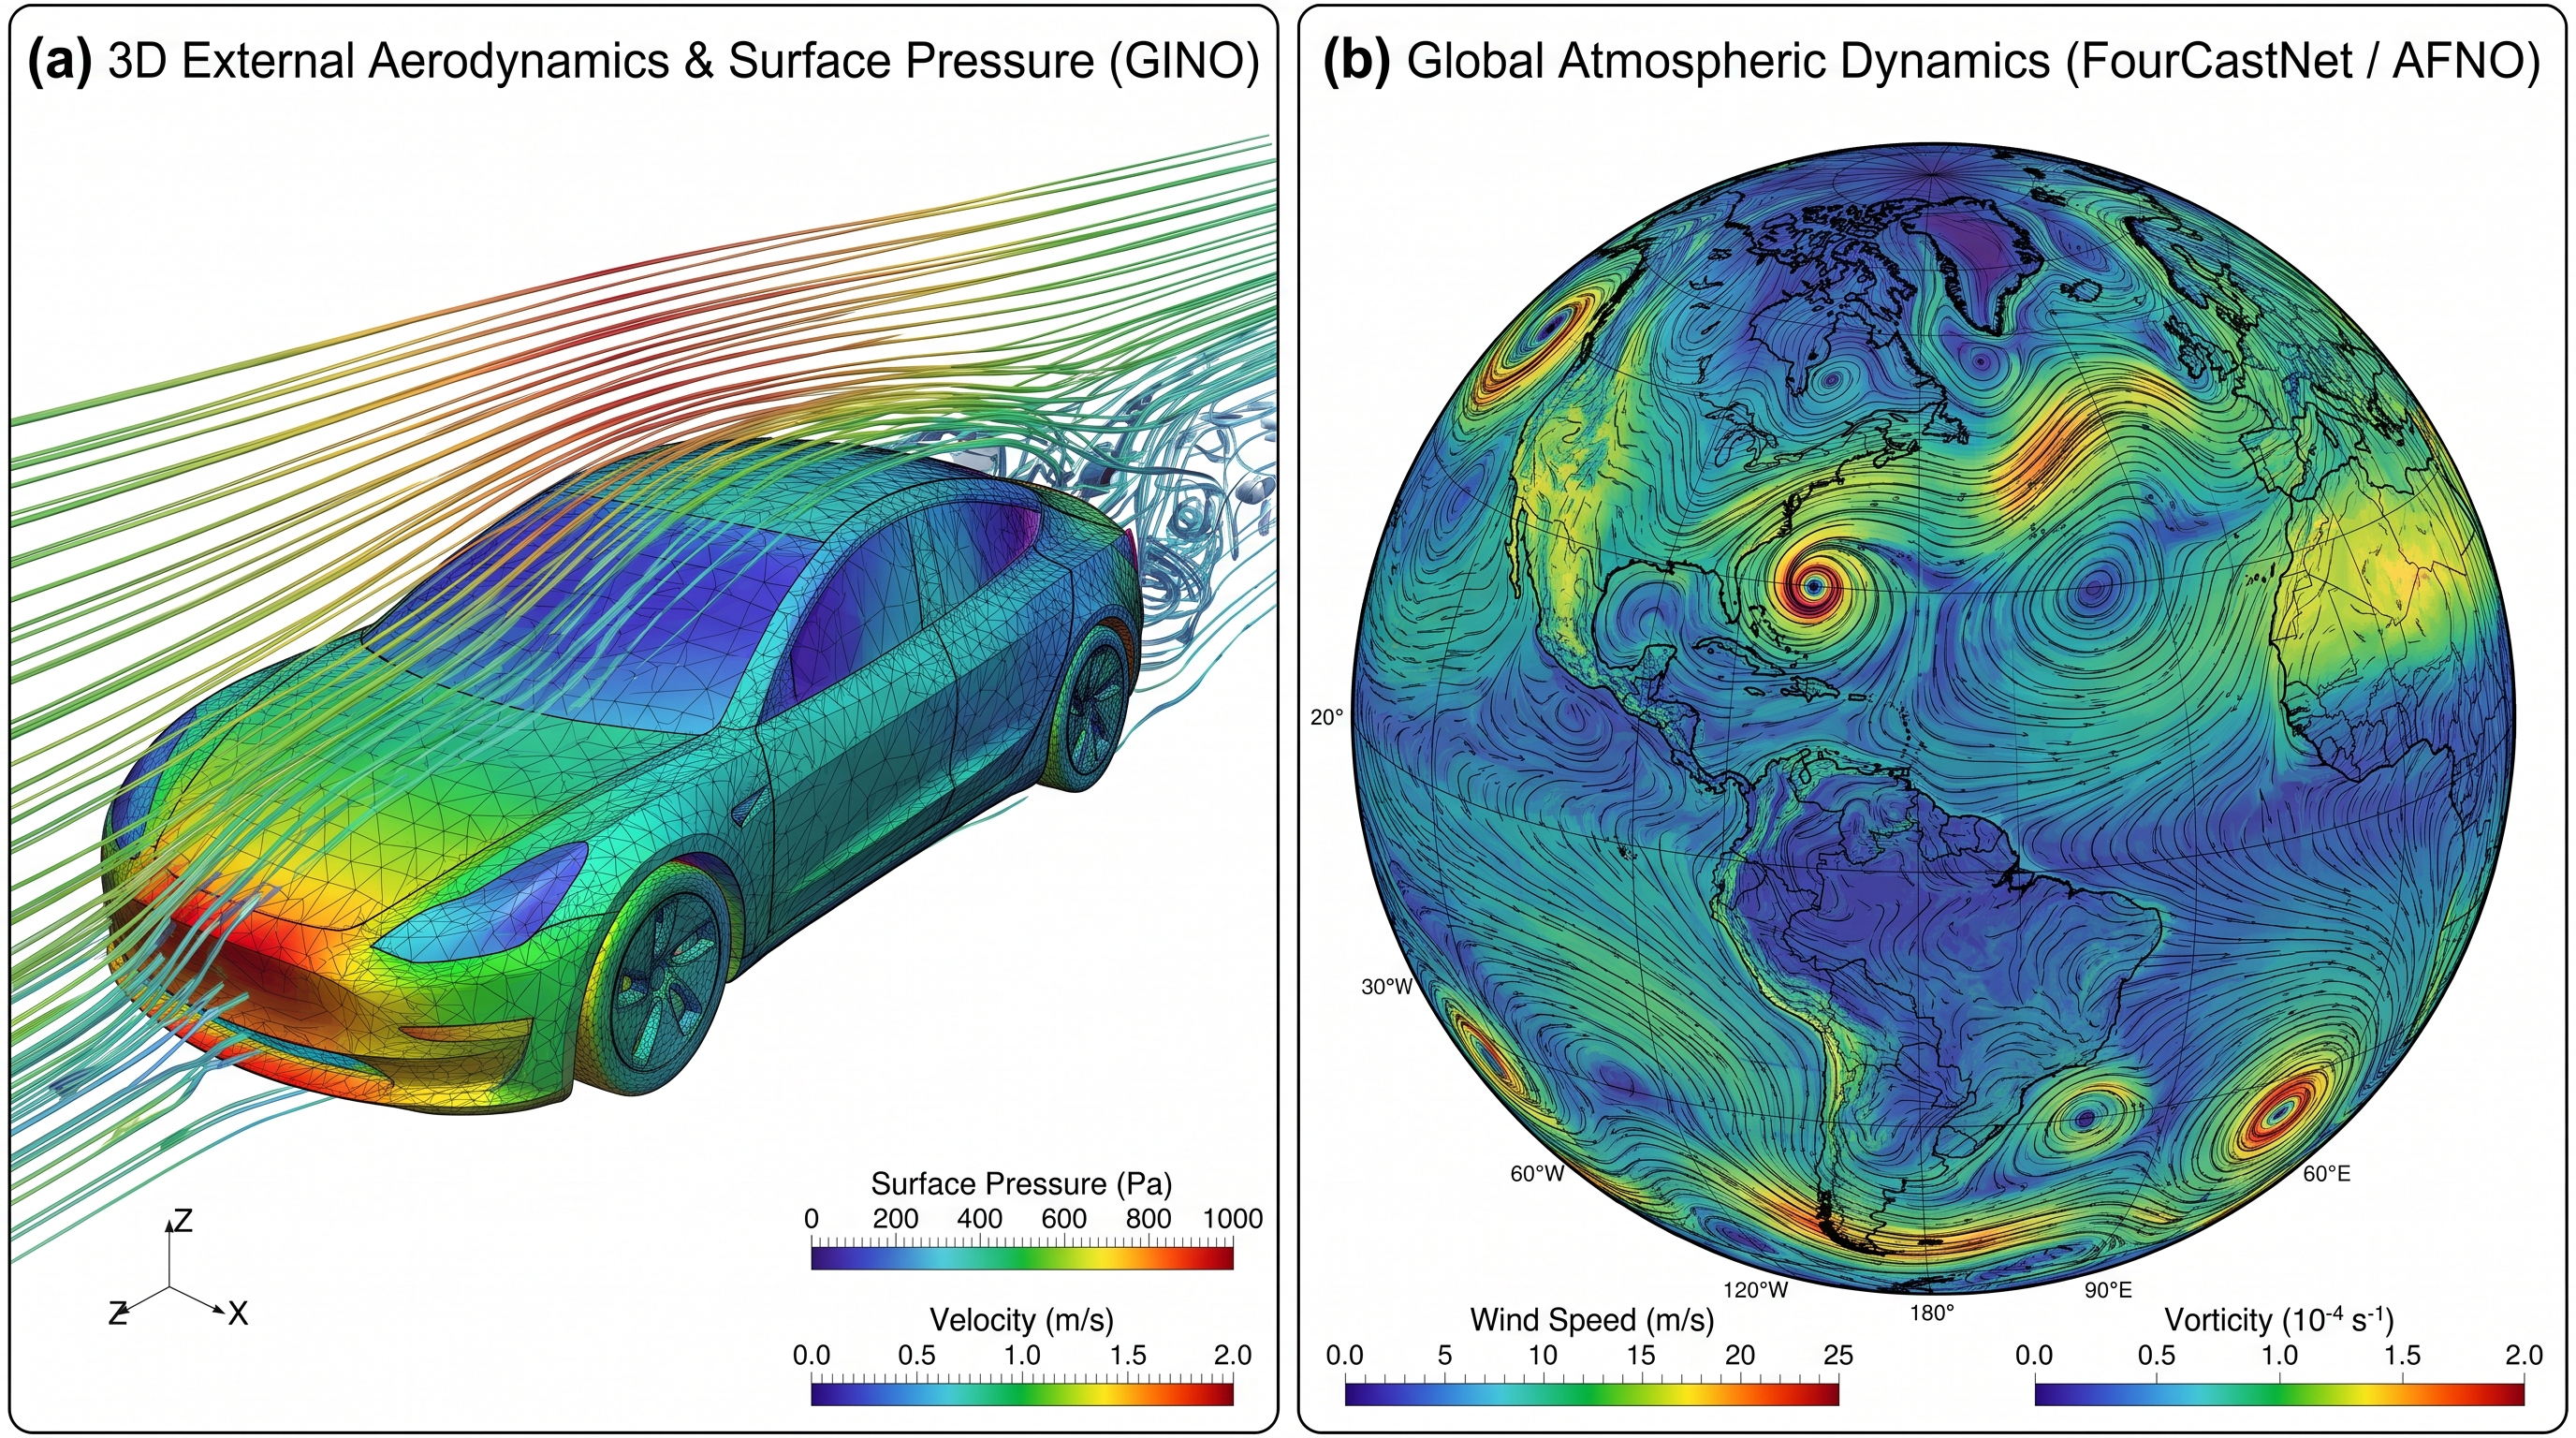
\includegraphics[width=0.95\textwidth]{fig_vol3_aerodynamics.jpg}
\caption{\textbf{Two-panel figure: surface pressure on a vehicle body (panel (a)) and global atmospheric structure (panel (b)).} Panel~(a), the subject of this chapter, renders the car body as its triangulated surface and colors it by predicted static pressure in pascals (color bar, $0$--$1000\ \mathrm{Pa}$); the external streamlines are colored by flow speed in meters per second (color bar, $0$--$2\ \mathrm{m\,s^{-1}}$), with the body axes at lower left. High pressure concentrates over the front bumper and hood, low pressure over the windshield and rear side window, and the flow detaches into a wake behind the base --- the front-to-base pressure difference that carries most of the drag on a bluff body. Panel~(b), the subject of \chapref{ch:part3-global-weather-forecasting-and-climate-dyn}, is a near-side view of the Earth with wind speed as shading and vorticity as contours, the fixed-sphere counterpart of the irregular geometry in panel~(a); it is cited from \chapref{ch:part3-global-weather-forecasting-and-climate-dyn} for that reading. Panel~(a) is an illustrative rendering of the output of a geometry-informed surface surrogate (GINO) of the type built in \chapref{ch:part2-graph-neural-operators-gno-and-irregular-g} and evaluated in Case Study~\ref{case:ch32-ahmed}; the two color bars beneath it are not mutually consistent and it is not a solver result.}
\label{fig:vol3_aero}
\end{figure}

Two further properties of the construction are aerodynamically useful and are worth stating
with their limits. The first is resolution behavior. GINO is discretization-convergent in the
sense of \cite{li2023geometry}: trained and tested at latent resolutions from $32$ to $88$, the
reported error is roughly flat, whereas a three-dimensional U-Net degrades at low resolution
because its receptive field shrinks with the grid; and trained on meshes sub-sampled by factors
of $2$ to $8$, the model evaluated on the full tessellation holds its error --- the zero-shot
super-resolution of \chapref{ch:part1-discretization-invariance-and-continuum-li} applied to a
surface rather than a volume. The caveat of that chapter transfers intact. Sub-sampling a mesh
thins the \emph{sampling} of a fixed smooth geometry; it does not remove geometric detail, and
the claim is therefore resolution transfer, not recovery of features absent from the coarse
input\index{zero-shot super-resolution!on surface meshes}.
The second is the alternative the
architecture did not take. Mesh-based message-passing solvers
\cite{brandstetter2022message} stay on the solver's own connectivity and never need a latent
box; GINO pays $\mathcal{O}(|E|)$ graph work --- $|E|$ the edge count of the two interface graphs
--- at two thin interfaces to buy a transform, and the
choice is exactly the one \chapref{ch:part2-graph-neural-operators-gno-and-irregular-g} prices.
For exterior aerodynamics the transform is worth it because the wake couples the base to the
far field, and a radius-$r$ graph layer needs many compositions to carry that interaction.

% -----------------------------------------------------------------------------
\section{Comparison with Classical Solvers (FVM / OpenFOAM)}
\label{sec:ch32-comparison}
% -----------------------------------------------------------------------------

The baseline is a finite volume method (FVM) code, and the framing should be precise about what
the method guarantees\index{finite volume method (FVM)!conservation identity}.
A finite volume discretization integrates the balance laws over each
control volume, so mass and momentum are conserved cell by cell as an algebraic identity of the
update, independently of whether the solution is accurate, with the boundary conditions entering
through face values and ghost cells rather than as constraints on a trial space
\cite{leveque2002finite}. Whether the resulting coupled algebraic system is solvable to accuracy is
a property of that system --- the stability analysis of the discrete problem, which for the
incompressible coupling is a mixed-formulation question \cite{quarteroni2008numerical} --- and not
something inherited automatically from the continuum problem. For \eqref{eq:rans} the
pressure--velocity coupling is handled
by a splitting algorithm --- the semi-implicit method for pressure linked equations (SIMPLE)
and its variants, or the pressure--implicit with splitting of operators (PISO) scheme for
transient problems --- and the steady state is reached by $1{,}500$ to $3{,}000$ such outer
iterations, each of which solves a linear system\index{SIMPLE and PISO pressure--velocity coupling}.
Two properties of that pipeline are what a design office buys, and neither is supplied for free
by a surrogate: the conservation identity, visible in residuals a certifier can inspect, and a
mesh-convergence study, the discipline's standard evidence that a reported $C_d$ is not an
artifact of the grid\index{mesh convergence study}.

The comparison is therefore not a single number but four axes: the labor that scales with
geometry, the wall-clock per query, the accuracy envelope and how it is measured, and
certifiability\index{surrogate!versus classical solver, axes of comparison}.
On labor, the solver pipeline is dominated by geometry intake --- computer-aided design (CAD)
cleanup, surface triangulation, boundary-layer prisms satisfying \eqref{eq:ch32-yplus}, volume
meshing, and quality checks on skewness and orthogonality --- and none of it amortizes, because
every candidate shape invalidates the mesh. The surrogate keeps the obligation in reduced form:
\eqref{eq:ch32-surrogate-map} still needs a tessellation and an $\mathrm{SDF}_{\mathcal{B}}$,
but a surface one rather than a volume one. On wall-clock, the attributed figure is
the 7--19 hours per geometry for label generation reported in Case
Study~\ref{case:ch32-ahmed}, against the
$2.6\times10^{4}$ ratio the cost--accuracy analysis of \cite{li2023geometry} reports for
computing drag coefficients relative to that same GPU OpenFOAM solver, measured as
the inference time needed to reach a $3\%$ relative error in $C_d$\index{cost--accuracy trade-off}.
Three qualifications make
that ratio usable. It is quoted against an optimized GPU solver run of the same case, not against
a conventional CPU solve, so the two wall-clock figures in circulation for this workload are not
interchangeable; the same work's
conclusion quotes a factor nearer $10^{5}$, and the book keeps the smaller, cost--accuracy-based
figure. It excludes meshing on both sides, though not the surrogate's own geometry intake: the
reported evaluation time includes computing the signed distance function, running the model, and
integrating the drag. And it is a ratio of times at matched accuracy, not a
statement that the surrogate is accurate --- the accuracy in question is the $3\%$ drag error at
which both curves are read. A tighter agreement with the volume solve, $1.2\%$, is also quoted for
this workload, but it is not a number \cite{li2023geometry} reports, and this chapter does not use
it.

% -----------------------------------------------------------------------------
\section{Amortization, the Pipeline Ledger, and Four Failure Modes}
\label{sec:ch32-ledger}
% -----------------------------------------------------------------------------

One arithmetic check belongs here, because this workload circulates with more than one wall-clock
pairing. A second, common in the applications literature, is a body-fitted mesh of order
$2\times10^{7}$ cells, a solve of $15$--$45$ minutes on 64 CPU cores, and a surrogate
evaluation of order ten milliseconds on an NVIDIA A100. That pairing is not the one behind the
number above, and it does not reconstruct it --- $9\times10^{2}\ \mathrm{s}$ over
$1\times10^{-2}\ \mathrm{s}$ is $9\times10^{4}$, not $2.6\times10^{4}$. Nor does it match the
device and cost the cited work states, which are a single NVIDIA V100 and $0.1\ \mathrm{s}$ per
shape, an order of magnitude above the ten milliseconds just quoted. The two figures differ because
their baselines, their hardware, and their accuracy targets all differ.
The rule the chapter follows throughout is that a
speedup travels with the baseline and the accuracy target that produced it, or not at
all\index{speedup ratios!baseline and accuracy target}.

What ties the first two axes together is amortization, where the arithmetic of
\chapref{ch:part2-production-deployment-and-high-throughput-} applies unchanged. If
$C_{\text{train}}$ is the offline cost of fitting
\eqref{eq:ch32-surrogate-map} --- several hundred solver runs at 7--19 hours each, the dominant
term by far --- and $C_{\text{eval}} \ll C_{\text{solve}}$ are the per-query costs, the
break-even query count is
\begin{equation}
  \label{eq:ch32-break-even}
  N_q^{*} = \frac{C_{\text{train}}}{C_{\text{solve}} - C_{\text{eval}}},
  \qquad
  \frac{C_{\text{train}}}{N_q} + C_{\text{eval}} \;\le\; C_{\text{solve}} \iff N_q \;\ge\; N_q^{*}.
\end{equation}
Equation \eqref{eq:ch32-break-even} is the honest form of the speedup claim: the
$2.6\times10^{4}$ factor is $C_{\text{solve}}/C_{\text{eval}}$, not the amortized ratio, and a
benchmark on a handful of held-out shapes never reaches $N_q^{*}$; a shape optimization loop over
thousands of variants
does, which is the workflow \chapref{ch:part3-the-multi-query-bottleneck-in-computationa}
enumerated\index{break-even query count}.
Table~\ref{tab:ch32-pipelines} sets the pipelines side by side, and two rows carry the remaining
axes. The error-reference row records that a solver's accuracy envelope is established by grid,
domain, and time-step refinement whereas the surrogate's is a comparison against a fixed set of
labels, so by the budget \eqref{eq:ch27-budget} the surrogate cannot be better than the fields it
was trained on; the certification row records what a reviewer may ask of each.

\begin{table}[htbp]
\centering
\small
\caption{\textbf{Two routes to a drag coefficient for one geometry.} Times and counts are those reported in \cite{li2023geometry} for the Ahmed-body configuration of Case Study~\ref{case:ch32-ahmed}; the $15$--$45$ minute CPU pairing discussed in the text is not from that source.}
\label{tab:ch32-pipelines}
\begin{tabularx}{\textwidth}{@{}>{\raggedright\arraybackslash}p{0.20\textwidth}>{\raggedright\arraybackslash}X>{\raggedright\arraybackslash}X@{}}
\toprule
\textbf{Stage} & \textbf{RANS volume solver (FVM)} & \textbf{GINO surface surrogate} \\
\midrule
Geometry intake & CAD cleanup, surface wrap, prismatic boundary-layer cells at $y^{+} \lesssim 1$ & surface tessellation plus $\mathrm{SDF}_{\mathcal{B}}$; no volume mesh \\
Unknowns & $\mathcal{O}(10^{7})$ cells, $\mathcal{O}(10^{5})$ surface nodes & $\mathcal{O}(10^{5})$ surface nodes at the interfaces; $64^{3}$ latent grid inside \\
Physics & \eqref{eq:rans} with closure \eqref{eq:ch32-reynolds-stress}, solved simultaneously & closure never solved; its effect is absorbed into the labels \\
Solve & SIMPLE-type outer iterations, linear solves per step, residual monitoring & one forward pass; cost per field as \eqref{eq:ch27-cost} \\
Output & volume field $(\mathbf{u},p,k,\omega)$ everywhere, plus surface integrals \eqref{eq:ch32-force-coeff} & surface fields $(p,\boldsymbol{\tau}_w)$ only; $C_d$ obtained by quadrature \\
Wall-clock per geometry & 7--19 h on 16 cores and 2 GPUs (label generation) & $0.1\ \mathrm{s}$ per shape on one NVIDIA V100; $2.6\times10^{4}\times$ faster at $3\%$ drag error \\
Error reference & grid, domain, and time-step convergence & relative $L^2$ on surface pressure, $7$--$8\%$ on the two families \\
Certification hook & conservation identity, inspectable residuals, mesh study & no conservation guarantee; requires the (model, mesh, metric) triple of \chapref{ch:part2-graph-neural-operators-gno-and-irregular-g} \\
\bottomrule
\end{tabularx}
\end{table}

What remains are the failure modes, and they are specific to this application. The first is
distributional. The Ahmed body is a simplified bluff body: its underbody
is flat, its wheels are usually idealized, and its mirrors, door gaps, and cooling flows are
absent. A surrogate trained on that family and asked about a production car with a detailed
underbody returns a plausible field, not an error message --- the out-of-distribution (OOD)
failure\index{out-of-distribution (OOD) failure!geometry families}
\chapref{ch:part2-production-deployment-and-high-throughput-} warns about, here with a geometry
rather than a coefficient field as the argument. The second is the closure. Where RANS with
\eqref{eq:ch32-reynolds-stress} mispredicts separation --- and the base pressure of a bluff body
is precisely where a scalar eddy viscosity is most suspect --- the labels carry the error and
\eqref{eq:ch27-budget} makes it irreducible by retraining on the same
grid\index{turbulence model error!label ceiling}. A surrogate can be
made cheap; it cannot be made more faithful to the physics than the model that generated its
data, and the honest comparison is therefore against wind-tunnel measurement, which is what
industry does and which no operator-learning result in this book addresses. The third is
conservation: \eqref{eq:ch32-surrogate-map} never forms a flux balance, so the cell-by-cell
identity that \cite{leveque2002finite} makes structural in the finite volume update has no
counterpart here, and the predicted
pressure and WSS fields need not integrate consistently with any divergence-free velocity ---
the gap \chapref{ch:part3-boundary-condition-enforcement-neural-oper} takes up. The fourth is
scope: anything downstream that needs the volume --- acoustics, thermal loading, a force on a
component inside the engine bay --- is outside \eqref{eq:ch32-surrogate-map} however well the
surface is predicted.

\takeaway{What the Aerodynamic Numbers License}{The reported result is a surface surrogate that
reaches a $3\%$ drag error in wall-clock shorter by a factor of $2.6\times10^{4}$ than an
optimized GPU RANS run, at $7$--$8\%$ relative $L^2$ error on the surface pressure field, for a
family of bluff bodies at $Re \le 6.82\times10^{6}$. It is not a certified replacement for a
convergence study, it does not extend across geometry families without new labels, and its
accuracy is bounded by the turbulence model that produced those labels.}

% -----------------------------------------------------------------------------
% Bridge to Chapter 3.3
% -----------------------------------------------------------------------------

Every limitation just listed has a counterpart in a different domain, and the next chapter
makes the contrast productive. External aerodynamics as treated here is a boundary-value
problem: the designer wants the solution \emph{at} the boundary, on a geometry that varies from
query to query, with no initial condition at all because the steady state is what is reported;
the surrogate's job is a shape-to-surface-field map evaluated once per shape. Global atmospheric
prediction inverts both parameters. The geometry is
fixed --- the sphere $\mathbb{S}^2$, the one case where the lattice and stationarity assumptions
that \chapref{ch:part1-the-fourier-neural-operator-spectral-theor} surrendered for a car body are
available again, although \chapref{ch:part3-global-weather-forecasting-and-climate-dyn} is careful
to note that the availability is not free, because an equiangular latitude--longitude grid is not
the sphere --- and the state evolves, so the operator is a time-stepper applied forty times in
succession for a ten-day forecast and the error question becomes the rollout question of
\chapref{ch:part1-open-theoretical-problems-and-mathematical}. There the multi-query budget is
not thousands of geometries but fifty perturbed initial states twice a day, the labels are not
solver runs but a reanalysis --- a data-assimilation system cycled through the observational
record --- and the acceptance metric is not a drag coefficient but a skill score evaluated at a
lead time. The label-ceiling objection raised above returns there in a harsher register: a
reanalysis is the output of a primitive-equation core plus a tuned parameterization package plus
an assimilation system, so a surrogate trained on it inherits three error sources at once and,
unlike a finite volume solve, cannot be audited term by term. The conservation half of the
objection is deferred to \chapref{ch:part3-boundary-condition-enforcement-neural-oper}, which
treats it as a property a learned map may be built to satisfy rather than one it inherits.

% -----------------------------------------------------------------------------

% Chapter 3.3: Global Weather Forecasting and Climate Dynamics
% Part III of the book.

\chapter{Global Weather Forecasting and Climate Dynamics}
\label{ch:part3-global-weather-forecasting-and-climate-dyn}
\label{sec:climate}
% -----------------------------------------------------------------------------

Global weather prediction is an initial-value problem on the spherical shell
$\Omega = \mathbb{S}^2 \times [0, z_{\text{top}}]$, and it differs from the aerodynamic
setting of \chapref{ch:part3-external-aerodynamics-and-surface-flows} in the one respect
that governs the whole error budget: nothing about its domain varies. The geometry is a
sphere of fixed radius, so the lattice and stationarity assumptions that
\chapref{ch:part1-the-fourier-neural-operator-spectral-theor} had to surrender for a car
body are available here again, and the transform machinery of Part~II applies without an
encoder or a decoder in front of it. What has become hard is the number of applications.
A ten-day forecast is forty successive uses of a six-hour map; an operational center
integrates an ensemble of some fifty members at each forecast cycle --- the fifty-member,
ten-day benchmark forecast that \cite{pathak2022fourcastnet} takes as its unit of cost
comparison --- and that is the multi-query budget
\chapref{ch:part3-the-multi-query-bottleneck-in-computationa} prices and which
\chapref{ch:part2-production-deployment-and-high-throughput-} notes is already spent
before any surrogate exists. \index{weather forecasting!as an operator problem}
\index{numerical weather prediction (NWP)}

The atmosphere also breaks the error accounting that Parts~I and~II assume. It is chaotic,
so the amplification factor $\Lambda_\theta$ defined in \eqref{eq:ch09-onesided} exceeds one
by an amount the leading Lyapunov exponents fix, the pathwise bound \eqref{eq:ch09-gronwall}
saturates at that rate, and two trajectories with nearly identical starting states separate
while sharing the same statistics; skill is therefore scored field-by-field at a lead
time, not along a trajectory. The labels are not solver output either. They are a
\emph{reanalysis} --- the optimal estimate of the observed history produced by cycling a
data-assimilation system through the observational record \cite{hersbach2020era5} --- so whatever the assimilated
model got wrong is inherited by the surrogate as ground truth. And the quantity a user
cares about is often the part of the field the loss suppresses: the tail of the wind-speed
distribution, the heaviest millimeters of rain, the mesoscale structure that an
area-integral skill score barely notices.

This chapter takes the four questions in order. Section~\ref{sec:ch33-primitive} states the
hydrostatic primitive equations, isolates the three structural features that decide the
design of anything that learns from them, and names the closure and the boundary data the
equations do not supply themselves. Section~\ref{sec:ch33-fourcastnet} builds the actual
surrogate, \textbf{FourCastNet} and its Adaptive Fourier Neural Operator backbone, from the
architecture of Part~II outward: data, state tensor, mixing layer, training procedure.
Section~\ref{sec:ch33-verification} reads the reported skill and cost numbers with their
provenance pinned down, including the distinction between a wall-clock ratio and an
aggregate node-time ratio. Section~\ref{sec:ch33-limits} collects the failures that the same sources
report --- smoothed small scales, underestimated extremes, no extrapolation to unseen
intensity --- and states plainly why none of them licenses a climate claim. The reader
should bring the mode budget \eqref{eq:ch05-modeset}, the rollout recursion
\eqref{eq:ch26-rollout}, and the pushforward objective \eqref{eq:ch26-pushforward}; the
chapter adds a domain, a data policy, and a verification metric, not new theory.

% -----------------------------------------------------------------------------
\section{Governing Hydrodynamic Primitive Equations}
\label{sec:ch33-primitive}
% -----------------------------------------------------------------------------

Atmospheric circulation at the scales that matter to a forecast is modeled by the
hydrostatic primitive equations on a rotating sphere:
\begin{align}
  \label{eq:ch33-momentum}
  \frac{D \mathbf{u}_h}{Dt} + f \hat{\mathbf{k}} \times \mathbf{u}_h &= -\frac{1}{\rho} \nabla_h p + \mathbf{F}_h, \\
  \label{eq:ch33-hydrostatic}
  \frac{\partial p}{\partial z} &= -\rho g, \\
  \label{eq:ch33-continuity}
  \nabla_h \cdot \mathbf{u}_h + \frac{\partial w}{\partial z} &= 0, \\
  \label{eq:ch33-pottemp}
  \frac{D \theta}{Dt} &= \frac{Q}{c_p} \left(\frac{p_0}{p}\right)^{R/c_p},
\end{align}
where $\mathbf{u}_h = (u, v)$ is horizontal velocity, $f = 2\Omega_{\text{rot}} \sin\phi$ is
the Coriolis parameter at latitude $\phi$ for planetary rotation rate $\Omega_{\text{rot}}$,
and $\theta$ is potential temperature. The remaining symbols are the horizontal gradient
$\nabla_h$ and divergence on $\mathbb{S}^2$, the local vertical unit vector
$\hat{\mathbf{k}}$, density $\rho$, pressure $p$, vertical velocity $w$, gravitational
acceleration $g$, the material derivative
$D/Dt = \partial_t + \mathbf{u}_h \cdot \nabla_h + w\,\partial_z$, specific heat at
constant pressure $c_p$, the gas constant for dry air $R$, a reference pressure $p_0$, and
the two forcing terms $\mathbf{F}_h$ and $Q$. The derivation and the scaling that justifies
each term are standard geophysical fluid dynamics \cite{vallis2017atmospheric}, and
\eqref{eq:ch33-momentum}--\eqref{eq:ch33-pottemp} are used here as the definition of what the
surrogate is being asked to imitate. \index{primitive equations!hydrostatic}
\index{Coriolis parameter}

Three structural features of \eqref{eq:ch33-momentum}--\eqref{eq:ch33-pottemp} decide the
design of anything that learns from them. The first is balance. Away from acoustic and
gravity-wave noise, \eqref{eq:ch33-momentum} is close to geostrophic balance,
$f\hat{\mathbf{k}}\times\mathbf{u}_h \approx -\rho^{-1}\nabla_h p$, and
\eqref{eq:ch33-hydrostatic} is hydrostatic balance, so the state is not an arbitrary
element of a high-dimensional space: the fast modes carry little of the information a
verification metric rewards. This is why the geopotential height at $500\ \mathrm{hPa}$,
a smooth mid-tropospheric proxy for the pressure field, is the conventional index of
forecast quality in Section~\ref{sec:ch33-verification}, and why a surrogate that nails it
can still be wrong about the surface winds a wind farm needs. The second is that
\eqref{eq:ch33-continuity} is a constraint rather than an evolution equation: it makes the
vertical velocity diagnostic, obtained by integrating the horizontal divergence, and it
holds the mass of each atmospheric column in balance with the flux through its walls.
Nothing in \eqref{eq:ch33-statemap} enforces it, so a learned state may satisfy
\eqref{eq:ch33-momentum} and \eqref{eq:ch33-pottemp} to within its loss while quietly
creating or destroying column mass --- the same defect
\chapref{ch:part3-boundary-condition-enforcement-neural-oper} prices for the aerodynamic
surrogate, but there invisible in a single field and here accumulating over forty steps.
The third is that \eqref{eq:ch33-momentum} and \eqref{eq:ch33-pottemp} are not closed.
$\mathbf{F}_h$ lumps subgrid momentum mixing and boundary-layer turbulence; $Q$ lumps
radiative transfer and the latent heat release of convection, both of which are driven by
processes orders of magnitude smaller than the $28\ \mathrm{km}$ cell of
Section~\ref{sec:ch33-fourcastnet} and are supplied by parameterization schemes rather than
by the equations themselves.
\index{geostrophic balance}\index{physical parameterization!convection and radiation}

The system is also incomplete in the ordinary boundary-value sense, and the omissions
matter for what can be learned. \eqref{eq:ch33-momentum}--\eqref{eq:ch33-pottemp} require an
initial condition on the shell plus side conditions: no flow through the ground, vanishing
vertical velocity at the model top, periodicity in longitude, regularity at the poles. The
vertical coordinate implicit in $z$ is not geometric height but a hybrid coordinate,
pressure-like aloft and conforming to orography near the surface, so the same symbol denotes
a different physical spacing at every level and the grid is baked into the archive the
surrogate reads. The state that determines the future is larger still than the five fields
displayed: surface temperature over land, sea ice, and ocean, soil moisture, and the
radiative environment all enter $\mathbf{F}_h$ and $Q$, which is why a working surrogate is
handed twenty coupled channels rather than the primitive variables alone.

The consequence for operator learning is worth stating exactly. A solution operator is
defined by a differential equation together with its closure; here the closure is a
collection of tuned, non-exact models whose errors are a leading contributor to precipitation
forecast error. So the map an atmospheric surrogate learns is not a partial
differential equation (PDE) $\to$ solution map in the sense of
\chapref{ch:part1-partial-differential-equations-as-solution}. It is
$\text{PDE} + \text{parameterization package} + \text{assimilation system} \to \text{analysis sequence}$,
and every later claim of ``accuracy'' in this chapter is accuracy against that composite.
A classical solver at least knows which of its terms produced an error. A single learned
map does not, and cannot be audited term by term --- an instance of the opacity that
\chapref{ch:part3-boundary-condition-enforcement-neural-oper} treats from the
conservation side.

% -----------------------------------------------------------------------------
\section{FourCastNet and Adaptive Fourier Neural Operators}
\label{sec:ch33-fourcastnet}
% -----------------------------------------------------------------------------

\textbf{FourCastNet}~\cite{pathak2022fourcastnet} parameterizes the atmospheric solution
operator using \textbf{Adaptive Fourier Neural Operators} (AFNO), the spectral token mixer
of Guibas et al.~\cite{guibas2021afno}, whose construction the FourCastNet paper sets out
alongside the model that uses it. Operating on
the spherical equispaced latitude--longitude grid from the \textbf{European Centre for
Medium-Range Weather Forecasts} (ECMWF) \textbf{ERA5} reanalysis dataset
\cite{pathak2022fourcastnet,hersbach2020era5} --- $720 \times 1440$ pixels, corresponding to
$0.25^\circ \approx 28 \text{ km}$ spatial resolution --- the model predicts 20 prognostic
atmospheric variables:
\begin{equation}
  \label{eq:ch33-statemap}
  \mathcal{G}_{\text{AFNO}} : \mathbf{X}(t) \in \mathbb{R}^{20 \times 720 \times 1440} \longmapsto \mathbf{X}(t + 6\text{ h}).
\end{equation}
Equation \eqref{eq:ch33-statemap} is the time-$\Delta t$ map of
\chapref{ch:part1-open-theoretical-problems-and-mathematical} with $\Delta t = 6\ \mathrm{h}$
and the state $\mathbf{X}$ a twenty-channel image on the sphere; a $K$-step forecast is
$\mathcal{G}_{\text{AFNO}}^{K}$ applied as in \eqref{eq:ch26-rollout}. Two bookkeeping
details matter for reproduction. The archived regular grid carries $721$ latitude nodes
because both poles are included, so the tensor the code actually reads is
$721 \times 1440 \times 20$; and ERA5's native horizontal grid is a \emph{Gaussian} grid,
re-interpolated to the regular latitude--longitude arrangement by the Copernicus Climate
Data Store service before training \cite{pathak2022fourcastnet}. The interpolation is
benign arithmetically and not benign physically: it is a low-pass operation applied to the
labels, and any claim about what the model resolves must be read against it. \index{ERA5 reanalysis}\index{FourCastNet}
\index{latitude--longitude grid!pole singularity}

The geometry of that grid is the reason the operator's global mixing is cheap and the
reason its fine scales are not isotropic. At $0.25^\circ$ in both directions, a cell is
$28\ \mathrm{km}$ wide in the meridional sense everywhere, while its zonal width shrinks as
$\cos\phi$: the row one step below the pole is roughly $120\ \mathrm{m}$ wide in longitude
while its meridional extent stays $28\ \mathrm{km}$, an aspect ratio near $2\times10^{2}$, and
the polar row itself --- the $721$st latitude node --- is $1440$ stored copies of a single
point.
A spectral layer on such an array is not a spectral layer on the
sphere, since the spherical Laplacian's eigenfunctions are spherical harmonics, whose
degree-$n$ energy sits on cells of increasingly anisotropic shape. Operational models
handle this with reduced grids or with spectral-transform methods on Gaussian grids; the
surrogate instead treats the field as a Euclidean image and inherits the anisotropy. This
is a genuine departure from the periodic-domain setting of
\chapref{ch:part1-the-fourier-neural-operator-spectral-theor}, where the lattice is uniform
by assumption, and it is one reason the small-scale results of
Section~\ref{sec:ch33-limits} come out as they do. \index{spherical harmonics!versus latitude--longitude grids}

The channels in \eqref{eq:ch33-statemap} are chosen to represent the instantaneous state
rather than to be complete. Surface wind components $U_{10}, V_{10}$ at $10\ \mathrm{m}$,
2-meter temperature $T_{2m}$, surface pressure and mean sea-level pressure; zonal and
meridional wind and geopotential height at $1000\ \mathrm{hPa}$; temperature, wind,
geopotential and relative humidity at $850$ and $500\ \mathrm{hPa}$; geopotential height at
$50\ \mathrm{hPa}$; and integrated total column water vapor (TCWV) --- twenty fields in
all. Total precipitation is deliberately \emph{not} among them: it is a six-hour
accumulated diagnostic, and a second AFNO model maps the backbone's output onto it, with a
final convolution and rectified linear unit appended so that negative rainfall cannot be
produced \cite{pathak2022fourcastnet}.
\index{precipitation!as a diagnostic head}

Inside, the mixer is the AFNO layer rather than the \textbf{Fourier Neural Operator} (FNO)
layer of \eqref{eq:fno_layer}. The $720 \times 1440$ frame is projected onto an $h \times w$
grid of patches of size $p \times p$, with $p = 8$ in the published configuration, each patch
embedded as a $d$-dimensional token; the
tokens are transformed along the patch indices by a two-dimensional discrete Fourier
transform, a two-layer perceptron with block-diagonal weights shared across all patches acts
on each frequency's token embedding, and the result is sparsified and returned to the patch
domain with a residual connection \cite{pathak2022fourcastnet,guibas2021afno}. The sparsification is the
adaptive part and is what distinguishes it from a fixed low-pass truncation:
\begin{equation}
  \label{eq:ch33-shrink}
  \tilde{z}_{m,n} = S_\lambda\!\left(\mathrm{MLP}\left(z_{m,n}\right)\right),
  \qquad
  S_\lambda(x) = \mathrm{sign}(x)\,\max\!\left(|x| - \lambda,\, 0\right),
\end{equation}
where $z_{m,n}$ is the token embedding at frequency index $(m,n)$, $\mathrm{MLP}$ is the
two-layer perceptron with block-diagonal weights just described, and $\lambda$ is the
sparsity-controlling threshold, listed as $10^{-2}$ in the published hyperparameters. Equation
\eqref{eq:ch33-shrink} retains the modes whose coefficients survive
shrinkage instead of retaining a box such as \eqref{eq:ch05-modeset} by construction, so
the frequency support is input- and channel-dependent rather than fixed; the number of
parameters does not scale with the number of patches, which is the resolution-invariance of
\chapref{ch:part1-discretization-invariance-and-continuum-li} as an architectural property
of the mixer. \index{adaptive Fourier neural operator (AFNO)!token mixing}
\index{soft-thresholding!in the spectral domain}

The engineering payoff of that choice is stated in the source paper in memory terms, and it
is one of the two reasons that paper gives for preferring a transformer-style backbone over a
convolutional one: at \eqref{eq:ch33-statemap} resolution the AFNO model's footprint is about
$10\ \mathrm{GB}$ at batch size one, whereas carrying a nineteen-layer convolutional network
previously trained at $32 \times 64$ over to the same frame would need roughly
$83\ \mathrm{GB}$, and its receptive field would have to grow with the grid. The other reason
is empirical rather than arithmetic: the authors report that their convolutional runs
``showed poor performance on capturing small scales over many time steps in auto-regressive
inference'' \cite{pathak2022fourcastnet}, which is why Section~\ref{sec:ch33-limits} has a
subject at all. Compare the spectral-layer costing of \eqref{eq:ch23-cost}: the
$\mathcal{O}(N\log N)$ mixing is the same object, but the alternative to paying it is not a
cheaper network, it is a deeper one.

Training uses hourly ERA5 snapshots subsampled to $00, 06, 12, 18\ \mathrm{UTC}$, with
$54{,}020$ training frames drawn from 1979--2015, $2{,}920$ validation frames from
2016--2017, and 2018 onward held out untouched as the out-of-sample test
set \cite{pathak2022fourcastnet}. The procedure is two-stage and should be
recognized from Part~II: a one-step pretraining on pairs
$\big(\mathbf{X}(k),\mathbf{X}(k+1)\big)$, then fine-tuning in which the model is rolled out
two steps on its own output and the loss is the sum of the two step errors. That is
pushforward training \eqref{eq:ch26-pushforward} in all but name, at $K=2$. The source states
the procedure without justifying it;
\chapref{ch:part2-training-regimes-optimization-and-failure-} supplies the justification,
which is exposure bias under the rollout recursion \eqref{eq:ch26-rollout}. End-to-end
training takes about sixteen hours on sixty-four NVIDIA A100 graphics processing units
(GPUs).
\index{pushforward regularization!two-step fine-tuning}

% -----------------------------------------------------------------------------
\section{Comparison with Classical Operational Weather Models (ECMWF IFS)}
\label{sec:ch33-verification}
% -----------------------------------------------------------------------------

The baseline is \textbf{numerical weather prediction} (NWP) with the ECMWF
\textbf{Integrated Forecasting System} (IFS), a spectral-transform dynamical core solving
\eqref{eq:ch33-momentum}--\eqref{eq:ch33-pottemp} with parameterized physics on a CPU
cluster. The comparison is made on the metric operational services already use. For a
forecast $\mathbf{X}$, a verification analysis $\mathbf{Y}$, and climatology
$\mathbf{C}$, the \textbf{Anomaly Correlation Coefficient} (ACC) is
\begin{equation}
  \label{eq:ch33-acc}
  \text{ACC} = \frac{\sum_{i,j} (\mathbf{X}_{ij} - \mathbf{C}_{ij}) (\mathbf{Y}_{ij} - \mathbf{C}_{ij})}{\sqrt{\sum_{i,j} (\mathbf{X}_{ij} - \mathbf{C}_{ij})^2 \sum_{i,j} (\mathbf{Y}_{ij} - \mathbf{C}_{ij})^2}},
\end{equation}
where the anomaly is the departure from a climatological mean, so that
\eqref{eq:ch33-acc} is blind to any additive bias in $\mathbf{X}$: a forecast displaced
uniformly from the analysis still scores one. The \textbf{root-mean-square error} (RMSE)
\index{root-mean-square error (RMSE)}
reported alongside it is the quantity such a displacement would move, which is why the two
are always quoted together. The conventional instance of \eqref{eq:ch33-acc} is the
geopotential height at $500\ \mathrm{hPa}$, one of the twenty channels of
\eqref{eq:ch33-statemap}: smooth, mid-tropospheric, and the standard proxy for the pressure
field aloft.
\index{anomaly correlation coefficient (ACC)}

Equation \eqref{eq:ch33-acc} as written is a sum over array indices, and on a sphere that
is a defect rather than a simplification: the same field scored on a finer longitude
spacing would receive a different number, because the sum weights a square kilometer near
the pole far more heavily than a square kilometer near the equator. This is the
grid-dependence that \chapref{ch:part1-discretization-invariance-and-continuum-li}
identifies in the loss, and the remedy is the same --- insert the quadrature weights of the
area element $\mathrm{d}A = R^2 \cos\phi\, \mathrm{d}\phi\, \mathrm{d}\lambda$:
\begin{equation}
  \label{eq:ch33-accw}
  \text{ACC}_w = \frac{\sum_{i,j} w_j (\mathbf{X}_{ij} - \mathbf{C}_{ij}) (\mathbf{Y}_{ij} - \mathbf{C}_{ij})}{\left(\sum_{i,j} w_j (\mathbf{X}_{ij} - \mathbf{C}_{ij})^2 \; \sum_{i,j} w_j (\mathbf{Y}_{ij} - \mathbf{C}_{ij})^2\right)^{1/2}},
  \qquad w_j = \cos\phi_j .
\end{equation}
The published FourCastNet verification uses \eqref{eq:ch33-accw}, together with the
correspondingly weighted RMSE, averaged over many
initial conditions spread through a full year so that seasonal variation in skill does not
enter as a bias \cite{pathak2022fourcastnet}. \index{area weighting!on the sphere}

What the numbers say, with the hedging the source itself supplies. ACC is a correlation
that decays with lead time, so a forecast horizon is whatever threshold one agrees to
cross; the FourCastNet authors report ACC above $0.6$ for TCWV beyond day eight, and state
that their predictions are comparable to the IFS on ACC and RMSE at lead times of up to
three days, after which ``predictions of all modeled variables lag
close behind IFS'' out to a week \cite{pathak2022fourcastnet}. The stronger version of the
claim --- that the surrogate matches the operational solver at short lead times for
large-scale variables while outperforming it for small-scale variables, precipitation among
them --- is also the authors' own, and it is a claim
about $\mathbf{X}$ against ERA5 at a fixed lead time, not about the statistics of a long
rollout. \index{forecast horizon!defined by a skill threshold}

Cost accounting requires the same care, because the ratio depends entirely on what is being
divided. The paper's own comparison is node-to-node for a $100$-member, $24$-hour ensemble:
the IFS at $18\ \mathrm{km}$ is estimated to need roughly $984{,}000$ node-seconds and about
$271\ \mathrm{MJ}$, while FourCastNet completes the same task in about $7$ node-seconds on
a single four-GPU node at roughly $8\ \mathrm{kJ}$, the IFS needing on the order of
$3{,}060$ nodes for the job. The resulting speedups are $145{,}000\times$ at the
$30\ \mathrm{km}$ the trained model runs at --- the paper's rounding of the
$0.25^\circ$ grid --- and $45{,}000\times$ for an $18\ \mathrm{km}$ realization of it, with
energy ratios of $24{,}000\times$ and $12{,}000\times$ respectively; the second of those two
speedups is an extrapolation rather than a
measurement, since no $18\ \mathrm{km}$ version of the model was ever trained and its
timing is obtained by interpolating data and parameters to that grid
\cite{pathak2022fourcastnet}. A second, far smaller ratio is the one usually repeated: a
week-long global forecast in under two seconds on one A100 --- $1.8\ \mathrm{s}$, the
figure this book carries; this book also quotes roughly two hours of
wall-clock for a single IFS member on a supercomputer cluster. Their ratio,
$7{,}200/1.8$, is the familiar $4{,}000\times$. That division is arithmetic on two different
machines, and the primary source does not report the elapsed time of one member on one
partition at all: its only wall-clock figure is for a whole ensemble, a $15$-day,
$51$-member IFS run on $1{,}530$ CPU nodes in $82$ minutes, from which the node-second
totals above are derived. This chapter therefore reads the $4{,}000\times$ as a statement
about latency on a device rather than as a costing. The two accountings answer different
questions, and the
difference between $4{,}000\times$ and $45{,}000\times$ is mostly the ensemble size divided
out. Table~\ref{tab:ch33-cost} sets them side by side. \index{speedup!wall-clock versus node-hour}
\index{European Centre for Medium-Range Weather Forecasts (ECMWF)}
\index{Integrated Forecasting System (IFS)}

\begin{table}[htbp]
\centering
\small
\caption{Two accountings of the same surrogate. Wall-clock ratios compare one forecast
member on one device; aggregate ratios compare the machine time of a whole ensemble.
Values as reported or estimated by \cite{pathak2022fourcastnet}; the per-member wall-clock
figures in the third row are the ones this book carries.}
\label{tab:ch33-cost}
\begin{tabular}{@{}>{\raggedright\arraybackslash}p{0.30\textwidth}>{\raggedright\arraybackslash}p{0.30\textwidth}>{\raggedright\arraybackslash}p{0.32\textwidth}@{}}
\toprule
\textbf{Quantity} & \textbf{ECMWF IFS} & \textbf{FourCastNet (AFNO)} \\
\midrule
State represented & $>150$ variables, $>50$ vertical levels & 20 variables at five levels, surface included \\
Time stepping & spectral-transform dynamical core and parameterized physics & learned six-hour map \eqref{eq:ch33-statemap} \\
Week-long global forecast & $\approx 2\ \mathrm{h}$ per member; $82$ min for a $15$-day $51$-member run on $1{,}530$ nodes & under $2\ \mathrm{s}$ ($1.8\ \mathrm{s}$ as quoted) on one A100 \\
$100$-member, $24$-h ensemble & $\approx 984{,}000$ node-s, $\approx 271\ \mathrm{MJ}$, $\approx 3{,}060$ nodes & $\approx 7$ node-s, $\approx 8\ \mathrm{kJ}$, one $4\times$A100 node \\
Aggregate speedup & --- & $45{,}000\times$ ($18\ \mathrm{km}$, extrapolated) to $145{,}000\times$ ($30\ \mathrm{km}$) \\
Energy ratio & --- & $12{,}000\times$ to $24{,}000\times$ lower \\
Development cost & decades of model development & $\approx 16\ \mathrm{h}$ on $64$ A100 GPUs; training energy $\approx$ one 10-day 50-member IFS forecast \\
\bottomrule
\end{tabular}
\end{table}

Table~\ref{tab:ch33-cost} makes the real argument of this chapter visible in one place: the
surrogate's advantage is not that it forecasts, which the IFS also does, but that it makes
ensemble size a free variable. The IFS reference run behind the accounting above is a
$51$-member ensemble, and every extra member costs another slice of a $1{,}530$-node
allocation; a thousand-member ensemble of a $7$ node-second model, by contrast, is an
accounting exercise rather than a project, and initial-condition perturbation by Gaussian
noise on the standardized state is enough to produce one \cite{pathak2022fourcastnet}.
Part~II's
throughput machinery of \chapref{ch:part2-production-deployment-and-high-throughput-} is
exactly what turns that arithmetic into a batch dimension. Panel~(b) of
Figure~\ref{fig:vol3_aero}, printed in \chapref{ch:part3-external-aerodynamics-and-surface-flows},
shows the object these numbers are attached to: the sphere. That plate's other panel,
(a), carries the vehicle surface treated in the present chapter; the two are printed
together there because they are the same transform applied to a domain that is fixed
and to one that is not.
\index{ensemble forecasting!cost of}


% -----------------------------------------------------------------------------
\section{Limits of the Operator Reading: Scale, Extremes, and Climate}
\label{sec:ch33-limits}
% -----------------------------------------------------------------------------

Panel~(b) of Figure~\ref{fig:vol3_aero} is also the first clue to what is missing. Its vorticity
contours are smooth and its jets are broad; nothing in that panel shows a squall line, a
frontal band, or the sub-structure of a precipitation field. The quantitative literature
agrees with the eye test. Bonavita's 2024 audit~\cite{bonavita2024limitations}, which examines FourCastNet alongside two
other leading learned forecasters, concludes that such models ``are not
able to properly reproduce sub-synoptic and mesoscale weather phenomena and lack the
fidelity and physical consistency of physics-based models,'' with consequences for the
interpretation of their forecasts and of their perceived skill. The mechanism is not
mysterious. A least-squares objective against a single future state estimates the conditional
mean of
that state given the input; the conditional mean of a field with sharp fronts is a smoothed
field, and repeated application of \eqref{eq:ch33-statemap} compounds the smoothing. This
is the same arithmetic as the coefficient-decay bound \eqref{eq:ch05-coefficient-decay},
with the learned shrinkage of \eqref{eq:ch33-shrink} in place of a hard mode box.
\index{mesoscale!under-resolved by learned forecasters}\index{conditional mean!smoothing toward}

The model's own authors measure the consequence for tails rather than asserting it. They
define a \textbf{relative quantile error} (RQE) over logarithmically spaced upper quantiles
$Q = \{1-10^{-1}, \dots, 1-10^{-4}\}$,
\begin{equation}
  \label{eq:ch33-rqe}
  \mathrm{RQE}(\ell) = \sum_{q \in Q} \frac{\mathbf{X}^{q}_{\text{pred}}(\ell) - \mathbf{X}^{q}_{\text{true}}(\ell)}{\mathbf{X}^{q}_{\text{true}}(\ell)},
\end{equation}
where $\mathbf{X}^{q}(\ell)$ is the $q$-th quantile of the field at lead-time index $\ell$,
so that a negative value records systematic under-prediction of extremes. Equation
\eqref{eq:ch33-rqe} trends negative for both the surrogate and the IFS on surface wind
speed --- a few percentage points, with negligible difference between them --- and much
more strongly for precipitation, where the reported under-prediction of the extreme
percentiles is roughly $35\%$ against roughly $15\%$ for the IFS
\cite{pathak2022fourcastnet}. The same paper reports that a $100$-member ensemble tracks
Hurricane Michael's position well over its four-day trajectory but fails to reproduce the
full extent of the sharp drop in minimum sea-level pressure between $36$ and $48\ \mathrm{h}$,
and its authors hypothesize
that the failure comes from processes the model does not represent, convective and radiative
among them. That is the
closure of Section~\ref{sec:ch33-primitive} reappearing as a forecast error. \index{relative quantile error (RQE)}
\index{extremes!under-prediction of}

Out-of-distribution intensity is a harder limit than under-prediction, because it is not a
bias one can correct. Sun et al., in a 2025 study~\cite{sun2025grayswan}, retrained FourCastNet four times
on the $1979$--$2015$ ERA5 record: once on all of it, and three times with Category~3--5
tropical cyclones removed either globally or over a single ocean basin. Tested on the
Category~5 cyclones of $2018$--$2023$, the versions give essentially unchanged global
verification skill, but the version trained without Category~3--5 storms anywhere cannot
forecast them: the model does not extrapolate from weaker storms present in the
data to stronger ones absent from it. For a hazard-planning user, this is the property that
matters, and no ACC reported at day five speaks to it. \index{out-of-distribution!gray-swan cyclones}

Finally, the distinction this chapter's title invites and its evidence does not support.
\eqref{eq:ch33-statemap} is fit to short-horizon transitions between analyzed states inside
a record spanning four decades of one forced realization of the climate system. Climate
questions are questions about the invariant measure of the dynamics and about its response
to a forcing the training record does not contain. Part~I's rollout analysis is explicit
that nothing licenses the extrapolation: the pathwise bound \eqref{eq:ch09-gronwall}
becomes vacuous once the Lyapunov growth is resolved, the useful requirement is an
absorbing or statistical one such as \eqref{eq:ch09-weak}, and a spatial correlation at one
lead time says nothing about whether $\mathcal{G}_{\theta}^{K}$ has the right attractor as
$K \to \infty$. A model that under-represents mesoscale
variance, as \eqref{eq:ch33-rqe} shows, will misrepresent the statistics of any quantity
that variance sets --- eddy heat transport, storm-track frequency, the intensity
distribution --- even while its day-three anomaly correlations are excellent. Data
availability compounds this: ERA5 is a product of an assimilation system that changed
across the record \cite{hersbach2020era5}, so a learned map trained on the whole archive fits a non-stationary
estimator as well as a non-stationary atmosphere. \index{weather forecasting!weather versus climate}
\index{climate emulation!not provided by weather surrogates}
\index{reanalysis!as training labels}

\takeaway{What the Weather Numbers License}{A learned six-hour state map on the sphere
reaches IFS-comparable anomaly correlation for large-scale variables out to about three
days, lags slightly behind thereafter, and makes a $100$-member daily ensemble roughly four
to five orders of magnitude cheaper in aggregate machine time. It does not resolve
sub-synoptic structure, it under-predicts precipitation extremes by about $35\%$, it cannot
extrapolate to cyclone intensities absent from its training record, and none of its skill
scores constitutes evidence about climate.}

% -----------------------------------------------------------------------------
% Bridge to Chapter 3.4
% -----------------------------------------------------------------------------

The atmospheric case is the cleanest in this book because its geometry never changes, and
that is precisely what makes its failures diagnostic: smoothing, tail under-prediction, and
distribution shift are properties of the learned map and the loss, not of an awkward
domain. Move the same three failures onto a domain where the geometry does change and where
the front is not merely under-resolved but genuinely discontinuous, and the difficulty
sharpens. \chapref{ch:part3-subsurface-multiphase-flow-and-carbon-stor} does exactly that.
There the operator maps a permeability field and an injection schedule to the saturation of
a supercritical phase --- lighter than the brine it displaces, which is why it rises ---
migrating through layered rock beneath a low-permeability seal,
over decades rather than days; the governing two-phase Darcy system has moving sharp
saturation fronts whose spectral coefficients decay like the slow tail of
\eqref{eq:ch05-coefficient-decay}, so a fixed mode budget is a worse approximation than the
one the atmosphere tolerates. The remedy taken up there is architectural rather than
statistical --- multi-resolution branches that restore the local detail a global transform
suppresses --- and the verification target changes with it, from a correlation against an
analysis to plume extent, front position, and pressure buildup at a well. The data regime
changes too: where the atmosphere supplied four decades of hourly global analyses, the
reservoir supplies a handful of core measurements and a stochastic geological prior, so the
multi-query budget of \chapref{ch:part3-the-multi-query-bottleneck-in-computationa} returns
as uncertainty quantification over permeability fields rather than as an ensemble of initial
conditions.

% -----------------------------------------------------------------------------

% Chapter 3.4: Subsurface Multiphase Flow and Carbon Storage
% Part III of the book.

\chapter{Subsurface Multiphase Flow and Carbon Storage}
\label{ch:part3-subsurface-multiphase-flow-and-carbon-stor}
\label{sec:subsurface}
% -----------------------------------------------------------------------------

Geological carbon storage is a forecasting problem that sits on the wrong side of
every budget a numerical simulator has. Carbon capture and storage (CCS) requires
injecting $\mathrm{CO}_2$, compressed into a supercritical fluid above its critical
point at roughly $31.0\,^\circ\mathrm{C}$ and $7.38\,\mathrm{MPa}$, into deep
saline aquifers, and then predicting where the gas saturation plume will be and how
far the reservoir pressure will have risen, on injection horizons of decades and
migration horizons of centuries.
\index{carbon capture and storage (CCS)}
The mechanism that makes the practice possible is what makes the prediction hard:
supercritical $\mathrm{CO}_2$ is substantially lighter than the brine it displaces,
so it rises until a low-permeability caprock stops it.
\index{caprock!containment role}
The questions a regulator or a nearby groundwater user asks concern that caprock,
the faults, and the abandoned wellbores: how far the pressure front travels, and
whether the plume reaches a leaky pathway.

Classical solvers strain under two pressures at once. The first is the equation
system: two-phase flow in a porous medium is nonlinear, coupled, and of mixed
elliptic--hyperbolic type, and its saturation fronts are genuine discontinuities
whose speed is set by a jump condition rather than by smooth characteristics. The
second is the workflow. Permeability is measured at a handful of well cores and
interpolated statistically in between, so no single simulation is a prediction; the
decision-relevant object is a distribution over outcomes, which means solving the
same problem thousands of times on different geological realizations. That is the
multi-query pattern of
\chapref{ch:part3-the-multi-query-bottleneck-in-computationa} in its purest form.

Parts~I and~II supply the machinery and, more importantly, the doubts. Part~I
gives the spectral layer \eqref{eq:fno_layer}, whose global path is a trigonometric
polynomial of fixed degree, and
\chapref{ch:part1-open-theoretical-problems-and-mathematical} establishes what that
costs at a jump. Part~II gives the training protocol and the permeability prior that
generates the data. This chapter works the mismatch out where it bites hardest, in
the U-Net-enhanced Fourier neural operator (U-FNO) of Wen et al.~\cite{wen2022ufno},
which adds a multi-scale path to the Fourier branch precisely because saturation
fronts are localized shocks. It then reads the reported numbers carefully --- what
each metric measures, what dispersion sits behind each mean, what the acceleration
factor actually prices --- and closes with the failure modes no accuracy figure
addresses: mass conservation, extrapolation beyond the training horizon, and the
boundary of the geological family a surrogate may be asked about.

% -----------------------------------------------------------------------------
\section{Governing Multiphase Darcy Equations}
% -----------------------------------------------------------------------------

Subsurface flow of immiscible fluids --- a water/brine phase $w$ and a
$\mathrm{CO}_2$ gas phase $g$ --- through a porous rock matrix is governed by
Darcy's law coupled to mass conservation. The phase fluxes are
\begin{equation}
  \mathbf{u}_\alpha(x,t) = -\,\frac{k_{r\alpha}(S_\alpha)}{\mu_\alpha}\,\mathbf{K}(x)\big(\nabla p_\alpha - \rho_\alpha \mathbf{g}\big), \qquad \alpha \in \{w, g\},
  \label{eq:ch34-flux}
\end{equation}
in which $\mu_\alpha$ is phase viscosity, $\rho_\alpha$ phase density,
$\mathbf{g}$ the gravitational acceleration vector, and
$k_{r\alpha}(S_\alpha) \in [0,1]$ the relative permeability of phase $\alpha$, the
factor by which the presence of the other phase reduces that phase's ability to
carry flow. Combining \eqref{eq:ch34-flux} with a balance of mass on each phase
gives
\begin{align}
  \phi \frac{\partial (\rho_w S_w)}{\partial t} &= \nabla \cdot \left( \rho_w \frac{k_{rw}(S_w)}{\mu_w} \mathbf{K} (\nabla p_w - \rho_w \mathbf{g}) \right) + q_w, \label{eq:ch34-cons-w}\\
  \phi \frac{\partial (\rho_g S_g)}{\partial t} &= \nabla \cdot \left( \rho_g \frac{k_{rg}(S_g)}{\mu_g} \mathbf{K} (\nabla p_g - \rho_g \mathbf{g}) \right) + q_g, \label{eq:ch34-cons-g}
\end{align}
subject to saturation completeness $S_w + S_g = 1$ and capillary pressure
relation $p_c(S_g) = p_g - p_w$. Here $\mathbf{K}(x)$ is the spatially
heterogeneous permeability tensor, $\phi(x)$ is porosity, $S_g$ is
$\mathrm{CO}_2$ saturation --- written $S_{\mathrm{CO}_2}$ in panel~(a) of
Figure~\ref{fig:vol3_sub} and in the reservoir-engineering literature --- and
$k_{r\alpha}$ are relative permeabilities modeled via the van
Genuchten~\cite{vanguchten1980closed} or Brooks--Corey curves, with $q_\alpha$ a source or sink term concentrated at the
well perforations.
\index{Darcy's law!multiphase form}
\index{relative permeability}
\index{capillary pressure!pressure-saturation closure}
\index{van Genuchten model}
\index{Brooks--Corey model}

Two structural features of \eqref{eq:ch34-cons-w}--\eqref{eq:ch34-cons-g} organize
everything that follows. The first is the split between the pressure and the
saturation. Introducing phase mobilities $\lambda_\alpha = k_{r\alpha}/\mu_\alpha$,
the total mobility $\lambda_t = \lambda_w + \lambda_g$, and the fractional flow of
the gas phase,
\begin{equation}
  f_g(S_g) = \frac{\lambda_g(S_g)}{\lambda_t(S_g)}, \qquad
  \bar{\rho}(S_g) = \frac{\lambda_w \rho_w + \lambda_g \rho_g}{\lambda_t},
  \label{eq:ch34-mobility}
\end{equation}
and summing the two balances, yields at each instant an elliptic equation for the
gas pressure whose coefficient is the full tensor $\lambda_t \mathbf{K}$: pressure
adjusts everywhere at once, which is why a point in the reservoir senses an
injection change hundreds of meters away within a step. Subtracting, and taking the
limit of incompressible phases, negligible capillary gradient, and constant
porosity, the saturation obeys a first-order conservation law
\begin{equation}
  \phi\,\frac{\partial S_g}{\partial t} + \nabla \cdot \big( f_g(S_g)\,\mathbf{u}_t \big)
  = \nabla \cdot \big( \lambda_g\big[\bar{\rho} - \rho_g\big]\mathbf{K}\mathbf{g} \big) + q_g,
  \label{eq:ch34-satlaw}
\end{equation}
with $\mathbf{u}_t = \mathbf{u}_w + \mathbf{u}_g$ the total Darcy velocity. The
second term on the right is buoyancy: because $\bar{\rho} > \rho_g$ and
$\mathbf{g}$ points downward, the corresponding correction to the gas flux,
$-\lambda_g[\bar{\rho}-\rho_g]\mathbf{K}\mathbf{g}$, points upward and drives gas
along whatever permeability pathways are open to it, which is the mechanism behind
the gravity override visible in panel~(a) of Figure~\ref{fig:vol3_sub}. Everything
difficult about \eqref{eq:ch34-satlaw} sits in the fractional flow \eqref{eq:ch34-mobility},
which is a strongly nonlinear function of saturation rising from $0$ at the
irreducible gas saturation to $1$ as the water phase becomes discontinuous and
immobile. In one dimension with a prescribed constant flux, \eqref{eq:ch34-satlaw}
reduces to the classical Buckley--Leverett problem, whose solution is not smooth at
all: the nonlinearity of $f_g$ makes characteristics converge, and the physical
solution is a shock travelling at the speed the jump condition assigns it,
\begin{equation}
  s\,\big[S_g\big] = \frac{\mathbf{u}_t \cdot \hat{\mathbf{n}}}{\phi}\,\big[f_g(S_g)\big],
  \label{eq:ch34-rh}
\end{equation}
where $[\,\cdot\,]$ denotes the jump across the front and $\hat{\mathbf{n}}$ its
unit normal. As with every conservation law, the jump condition is not sufficient:
the compressive, entropy-admitting solution is the physically correct one, and the
finite-volume literature is the reference for that selection
\cite{leveque2002finite}.
\index{fractional flow}
\index{Buckley--Leverett solution}
\index{gravity override}
\index{Rankine--Hugoniot condition!saturation front}

The system displayed above is the textbook immiscible form, and the data used by
Wen et al.~\cite{wen2022ufno} come from somewhere richer: a full-physics simulator
in which phase densities, porosity, and the solubility of $\mathrm{CO}_2$ in brine
are nonlinear functions of pressure, so the generated system is compressible and
slightly miscible. This bears on interpretation. A neural operator trained on
simulator output approximates the map the simulator implements, including its
constitutive assumptions and its numerical dissipation, and inherits the
simulator's authority rather than the continuum model's. The residual
$\phi\,\partial_t(\rho_\alpha S_\alpha) + \nabla\cdot(\rho_\alpha\mathbf{u}_\alpha) - q_\alpha$
of \eqref{eq:ch34-cons-w}--\eqref{eq:ch34-cons-g} that a physics-informed penalty
such as \eqref{eq:pino_loss} would charge the network against is, here, a statement
about the idealized equations of this section and not about the labeled data.

% -----------------------------------------------------------------------------
\section{The U-FNO Architecture for Multiphase Flow}
% -----------------------------------------------------------------------------

Standard Fourier neural operator (FNO) models struggle when applied directly to
multiphase transport because $\mathrm{CO}_2$ saturation fronts form localized,
sharp saturation shocks. The U-FNO model of Wen et al.~\cite{wen2022ufno}
integrates multi-scale contracting and expanding residual blocks (U-Net topology)
with Fourier spectral convolution layers. The reason that
combination is the right one is not a matter of tuning. Each layer of the plain
architecture \cite{li2021fourier} has a global branch that is exactly a
trigonometric polynomial of degree $k_{\max}$, as \eqref{eq:fno_layer} makes
clear, and \eqref{eq:ch09-jump-tail} of \chapref{ch:part1-open-theoretical-problems-and-mathematical}
prices what a jump costs such a representation: the truncated spectral tail of a
discontinuity decays only like $k_{\max}^{-1/2}$, the field lies in $H^s$ for
$s < \tfrac12$ and no better, and \eqref{eq:ch09-gibbs} shows the partial sums
overshooting the jump by a fixed $8.9\%$ of its height in a layer whose width
shrinks but whose amplitude does not. A front is not a hard case at the margin of
the theory; it is the case the theory excludes.
\index{U-FNO (U-Net-enhanced Fourier neural operator)!motivation}
\index{Gibbs phenomenon!in saturation fronts}

The U-FNO layer keeps the global branch and adds a second, local one,
\begin{equation}
  v_{\ell+1} = \sigma\Big( W_\ell v_\ell + \mathcal{F}^{-1}\!\big(R_{\phi,\ell}\,\mathcal{F}v_\ell\big) + b_\ell + \mathcal{U}_\ell(v_\ell) \Big),
  \label{eq:ch34-layer}
\end{equation}
where $\mathcal{U}_\ell$ is a two-step downsample--process--upsample block with a
skip connection, run in parallel with the spectral path rather than in series with
it. The division of labor is the point: the spectral branch carries the long-range
elliptic pressure response, which is smooth and which a global basis represents
efficiently, while the U-Net path carries the front, whose content is concentrated
on $O(1)$ basis functions per scale rather than spread over all
$O(k_{\max})$ --- the asymmetry \eqref{eq:ch09-jump-tail} makes precise and which a
localized multiscale representation exploits. Concretely, the reported model treats
space \emph{and} time as a three-dimensional grid, applying a 3D Fourier operator
over $(r, z, t)$ on a field of $96 \times 200$ cells with 24 output snapshots, and
padding the array once at the network input --- and stripping the pad before the
projection --- because the physical boundaries, no-flow top and bottom and a closed
outer edge, are not periodic. The padding is a workaround
for the torus hypothesis of \eqref{eq:fno_layer}, not a discharge of it, and it is
the same device that appears in the benchmark implementations of
\chapref{ch:part2-canonical-pde-benchmarks-and-reference-wor}.
\index{padding!for non-periodic boundaries}

Inputs are the radial and vertical permeability fields, the porosity field, and the
injection-interval perforation map, broadcast alongside five scalars --- initial
reservoir pressure, reservoir
temperature, injection rate, a capillary-pressure scaling factor, and irreducible
water saturation --- plus channels carrying the radial, vertical, and temporal cell
coordinates. Two separate networks are trained, one returning gas saturation
$S_g$ and one returning pressure buildup $\mathrm{d}P$, each at 24 gradually
coarsening time snapshots over a 30-year injection at rates between 0.2 and
2~Mt/yr into a reservoir of thickness between 12.5 and 200~m and radius 100~km
\cite{wen2022ufno}. Because reservoir thickness varies across cases, cells outside
the formation are zero-padded and the objective is evaluated only over the active
cell set $\mathcal{V}_{\mathrm{act}}$,
\begin{equation}
  \mathcal{L}(\theta) = \mathbb{E}_{a \sim \mu}\left[\left(\frac{\sum_{j \in \mathcal{V}_{\mathrm{act}}} \big| z_\theta(x_j) - z^{\dagger}(x_j) \big|^{2}}{\sum_{j \in \mathcal{V}_{\mathrm{act}}} \big| z^{\dagger}(x_j) \big|^{2}}\right)^{1/2} + \beta \left(\frac{\sum_{j \in \mathcal{V}_{\mathrm{act}}} \big| \partial_r z_\theta(x_j) - \partial_r z^{\dagger}(x_j) \big|^{2}}{\sum_{j \in \mathcal{V}_{\mathrm{act}}} \big| \partial_r z^{\dagger}(x_j) \big|^{2}}\right)^{1/2}\right],
  \label{eq:ch34-loss}
\end{equation}
where $\partial_r$ is the derivative along the radial coordinate and $\beta$ a
weighting hyperparameter. The first term is the masked form of the relative $L^2$
loss of \eqref{eq:rel_l2_loss}; the second has no counterpart there, and the study
reports it as what sharpens the leading edge of the plume and the steep pressure
buildup near the injector. Masking matters here more than it usually does: the
reservoir thickness varies from case to case, so in the thin cases most of the array
is padding whose true value is zero, and an unmasked average dilutes the error the
network is being asked to reduce --- the reported reason for the masked scheme is
its better distribution of gradient signal.
\index{active-cell masking}
\index{derivative-weighted loss}

Panel~(a) of Figure~\ref{fig:vol3_sub} renders the physical setting these numbers
describe, and its conclusion is geometric rather than quantitative. On a section 4~km wide and
600~m deep, the plume does not spread as a radial ring: it rises off the well tip,
is arrested beneath the lower-permeability layer that caps the reservoir, and then
spreads laterally along the dipping bed downdip to the right, the outermost 30-year
contour reaching a distance coordinate of about 3.5~km, some
1.9~km beyond the well, while the near-well core stays saturated close to
$S_{\mathrm{CO}_2} = 1$. The features that decide containment --- the caprock, the
fault cutting the left flank of the plume, the wellbore itself --- are precisely
the ones a surrogate could smear across a few grid cells and still score well on an
interior field average, and the outermost contour, not the plume interior, is what
a monitoring question is about. That outermost contour is also the least well
resolved object in the field, which is the tension this architecture is designed
against.

\begin{figure}[t]
\centering
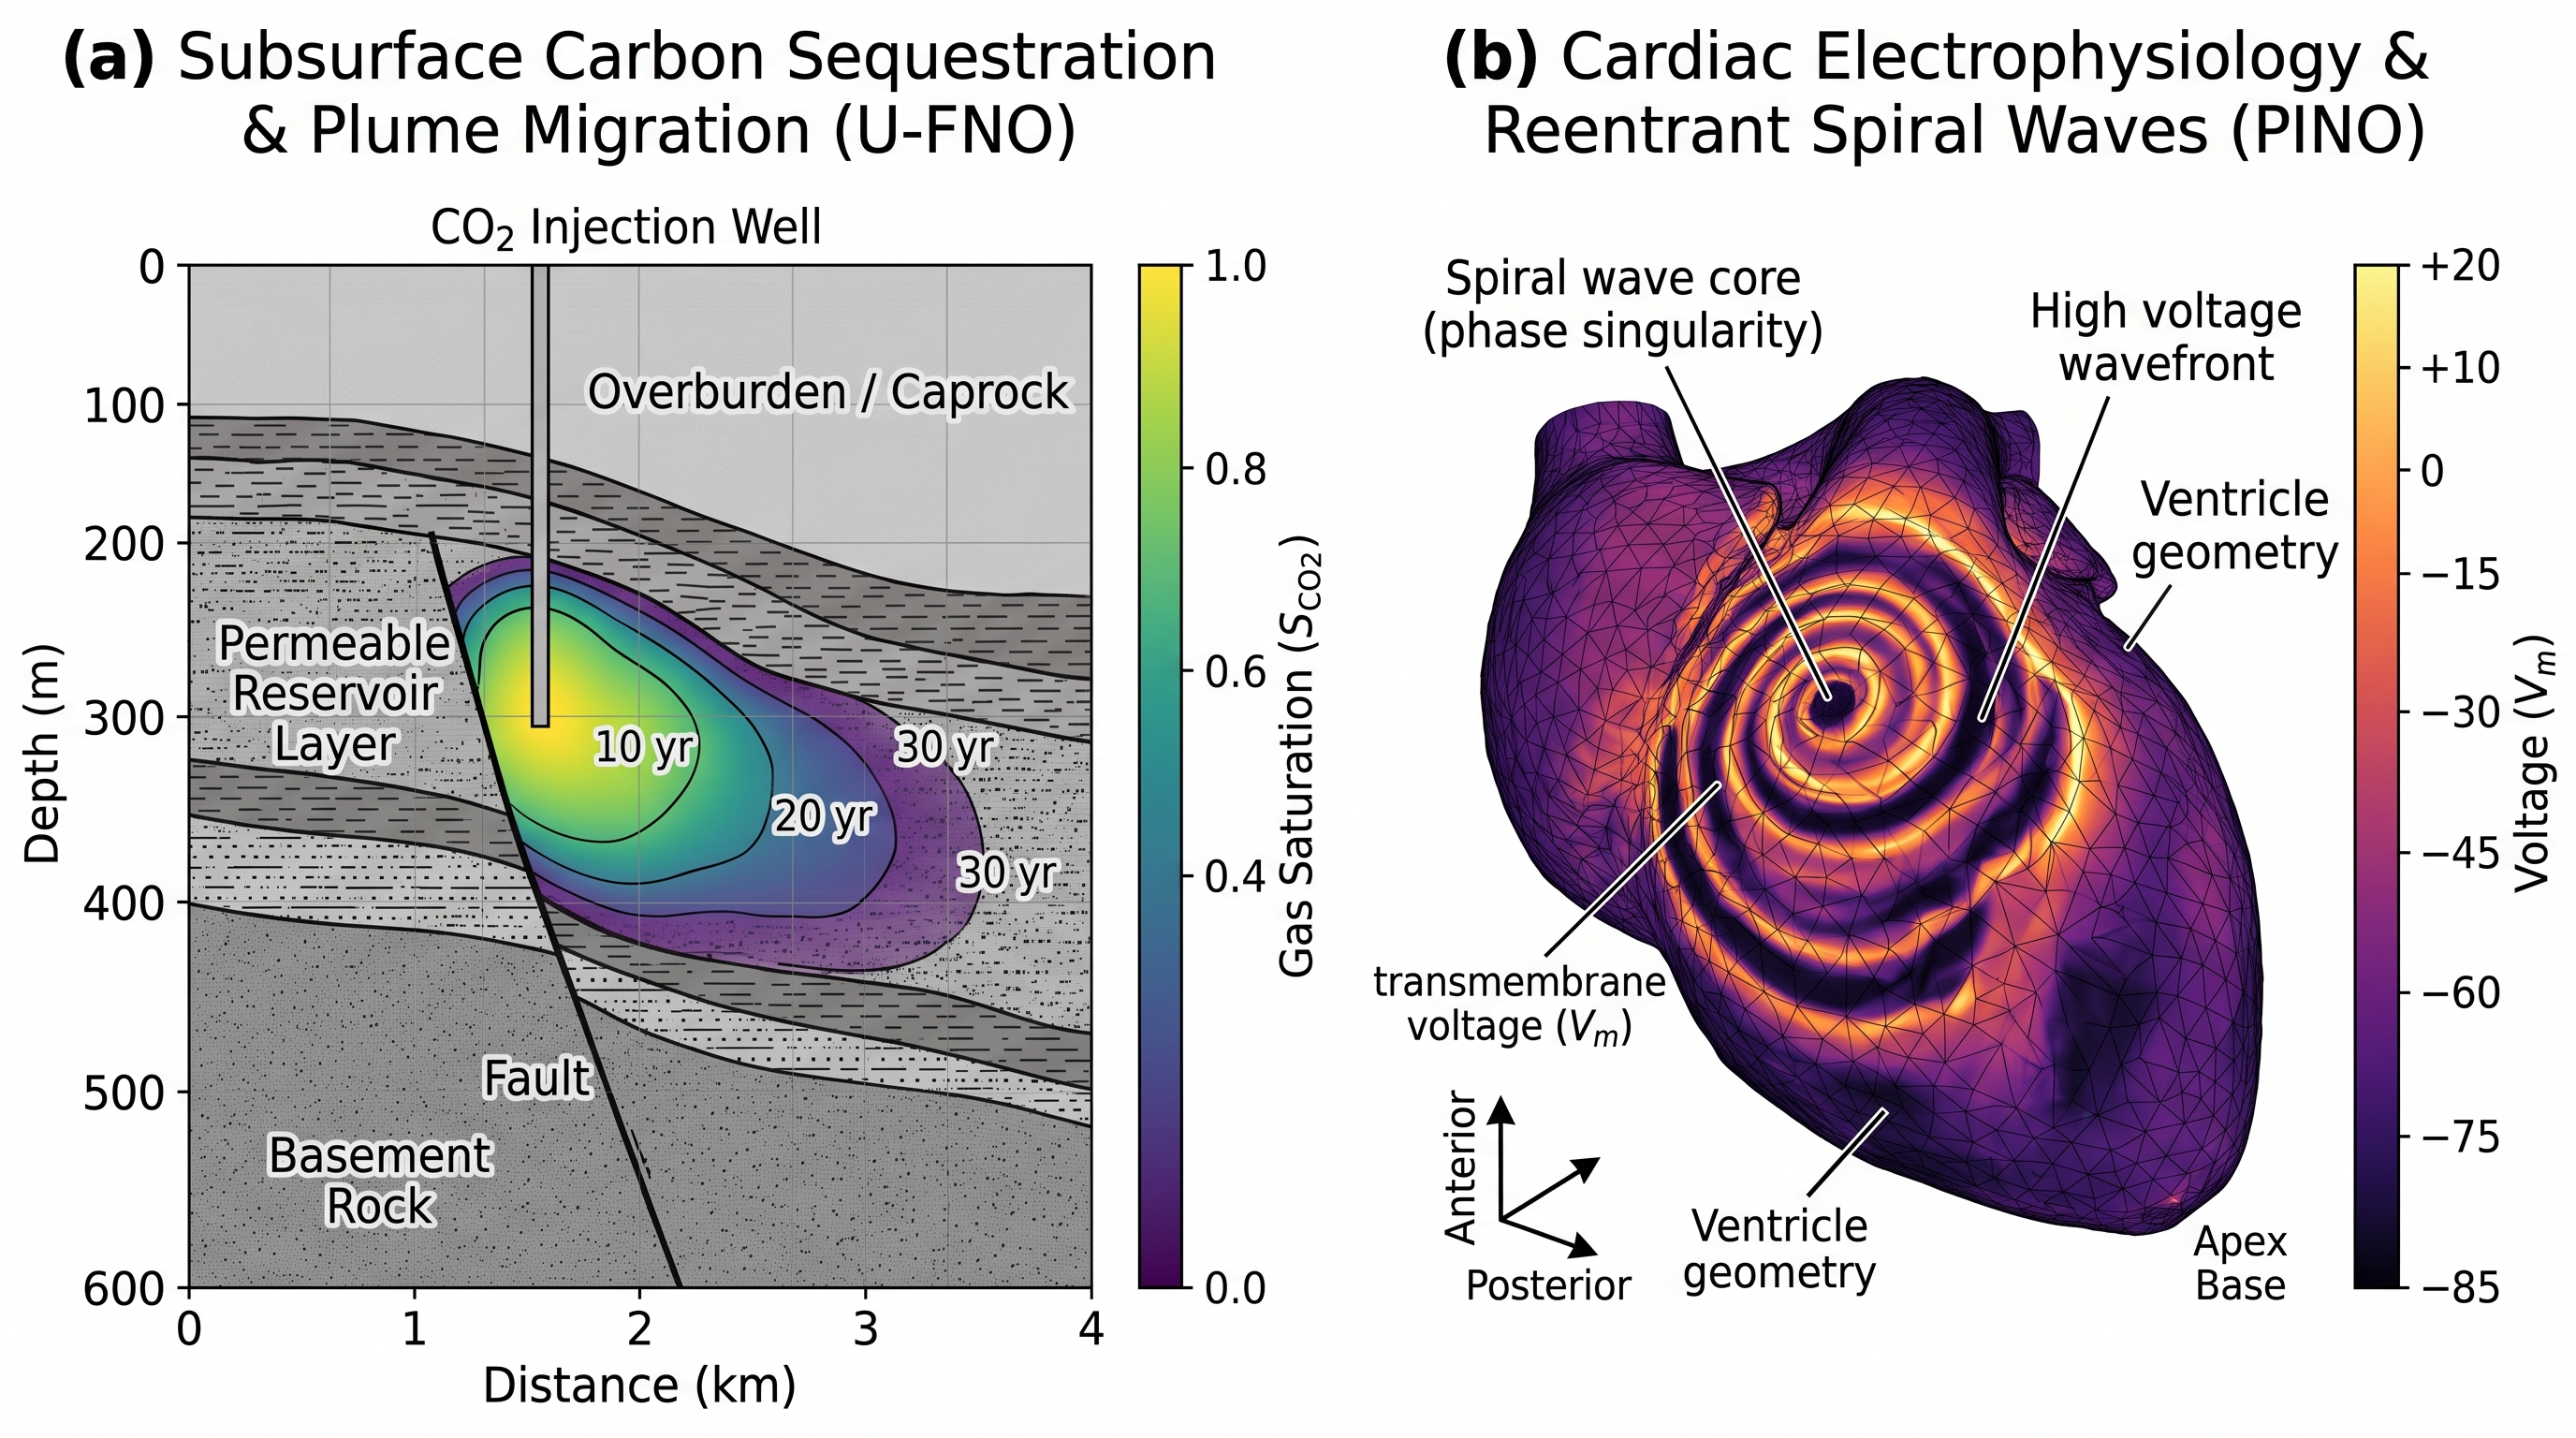
\includegraphics[width=0.80\textwidth]{fig_vol3_subsurface.jpg}
\caption{\textbf{Two-panel figure: subsurface $\mathrm{CO}_2$ plume migration
(panel~(a)) and cardiac reentrant spiral waves (panel~(b)).} Panel~(a), the
subject of this chapter, is a schematic cross-section of a saline-aquifer
$\mathrm{CO}_2$ storage site of the kind the U-FNO surrogate is trained to
simulate. Horizontal axis: distance, 0 to 4~km. Vertical axis: depth, 0 to
600~m, increasing downward. An impermeable overburden/caprock lies above
$\sim$110~m, a permeable reservoir layer between roughly 190 and 400~m, basement
rock below; a fault dips from 1.1~km at 200~m depth to the base of the section
near 2.2~km, and a vertical injection well enters at 1.6~km and terminates near
300~m. Filled contours give gas saturation $S_{\mathrm{CO}_2}$ on the scale 0 to
1; black contour lines mark the leading edge of the plume after 10, 20, and 30
years. Panel~(b), the subject of
\chapref{ch:part3-cardiac-electrophysiology-and-arrhythmia-d}, shows a reentrant
spiral wave of transmembrane voltage on a ventricle-shaped body rendered as a
triangular surface mesh, its colorbar labeled in millivolts from $-85$ to $+20$,
annotated at the spiral-wave core, the high-voltage wavefront, and the
anterior--posterior and apex--base axes; it is cited from
\chapref{ch:part3-cardiac-electrophysiology-and-arrhythmia-d} for that reading. Panel~(a) illustrates the physical
setting and the qualitative migration pattern; it is not a reproduction of a
figure from \cite{wen2022ufno}, whose benchmark is a two-dimensional radial
$(r,z)$ model without faulting, and no error figure quoted in this chapter is
read from either panel.}
\label{fig:vol3_sub}
\end{figure}
\index{plume migration!buoyant rise and lateral spreading}
\index{geological fault!as a leakage pathway}

% -----------------------------------------------------------------------------
\section{Performance vs. Classical Reservoir Solvers (Finite Difference)}
% -----------------------------------------------------------------------------

The baseline is not a straw solver. Commercial reservoir simulators of the class
used to generate the training data --- Eclipse, CMG, and the open-source research
toolkit MRST --- solve the coupled nonlinear system
\eqref{eq:ch34-cons-w}--\eqref{eq:ch34-cons-g} implicitly in time, with an
adaptive or fully implicit method (FIM) in which each step requires the residual
and its Jacobian and a Newton--Raphson iteration to convergence, upstream weighting
for the mobility, and a time-step controller that shortens steps whenever the
nonlinear solver struggles \cite{quarteroni2008numerical}. Wen et
al.~\cite{wen2022ufno} generated their data with the full-physics finite-difference
simulator Eclipse (e300) and report an average run time of about 10~min per
30-year case on one dedicated Intel Xeon E5-2670 core, each simulation using a
fully dedicated processor; the wider 10 to 30~min range per realization that this Part
carries forward is the working envelope for this class of problem. Against that, the trained U-FNO evaluates the same 30-year
evolution at 24 snapshots in 0.01 seconds on an NVIDIA A100 graphics processing
unit (GPU), for a reported 60,000$\times$ computational acceleration, with 1.6\%
gas saturation plume error and 0.68\% pressure error \cite{wen2022ufno}.
\index{fully implicit method (FIM)}
\index{reservoir simulator!Eclipse, CMG, MRST}

Those two percentages deserve to be read as what they are. In the study, 1.6\% is
the mean over 500 held-out cases of a mean absolute error computed \emph{inside the
separate-phase plume} --- the region where either the truth or the prediction is
nonzero --- and the accompanying standard deviation is about 1.1 percentage points;
0.68\% is the mean field relative error in pressure buildup, with a standard
deviation near 0.45. Neither number is a worst-case bound, and reporting the
plume error as ``below 1.6\%'' would misdescribe a distribution whose spread is
two-thirds of its center. The comparison against the plain FNO is more
informative still, because it shows what the U-Net path buys and what it costs. At
essentially the same parameter count, the plain FNO reaches a test plume error near
2.8\% and evaluates in about 0.005~s, while U-FNO reaches 1.6\% in 0.010~s: the
multi-scale path cuts the front error by roughly 40\% and doubles the inference
time, and the convolutional benchmark requires about three times the training data
to match the U-FNO's accuracy \cite{wen2022ufno}. The acceleration factor is
therefore not the largest available, and the architecture's claim is not speed but
speed at the accuracy where the physics concentrates.
\index{accuracy metrics!plume mean absolute error}
\index{speedup!as a property of the comparison setup}

Table~\ref{tab:ch34-cost} assembles the accounting, including the cost side that
an inference-time speedup invites the reader to forget. The speedup is a ratio of
two wall-clock numbers measured on specific hardware, and it moves when either
moves: the study itself notes that faster CPUs are available but would not
materially change the conclusion, which is true of the qualitative gap and false of
the factor --- a baseline twice as fast halves it. What does not depend on the
hardware is the shape of the cost curve. Simulation cost becomes a one-time
training cost plus a per-query cost four orders of magnitude or more below the
simulator's, and the data-generation cost is paid once and amortized across every
subsequent query. One qualification on the arithmetic: the $0.01$~s figure prices a
single network, and saturation and pressure are returned by two of them, so a query
that needs both fields costs about $0.02$~s and the honest ratio against a
$10$~min solve is nearer $3\times 10^{4}$ than $6\times 10^{4}$. The order of
magnitude is what the argument rests on, and it survives; the headline digit does
not.

\begin{table}[htbp]
\centering
\small
\caption{Cost and accuracy accounting for the U-FNO surrogate against the
finite-difference simulator that generated its training data, as reported by Wen et
al.~\cite{wen2022ufno} except that the 10--30~min run-time range is a figure this
Part carries without a primary reference. Simulator times are averages over 1,000 cases on one
dedicated Xeon core; surrogate times are averages over 500 held-out cases on one
A100 GPU, and the gas-saturation and pressure-buildup networks are evaluated
separately, so predicting both fields costs about twice the quoted 0.01~s.
Ensemble and training-set figures are arithmetic on the reported per-case costs,
not additional measurements.}
\label{tab:ch34-cost}
\begin{tabularx}{\textwidth}{l>{\raggedright\arraybackslash}X>{\raggedright\arraybackslash}X}
\toprule
 & \textbf{Implicit finite-difference simulator} & \textbf{U-FNO surrogate} \\
\midrule
Object computed &
  Cell-centered solution of \eqref{eq:ch34-cons-w}--\eqref{eq:ch34-cons-g}, every step &
  Approximate solution operator fitted on simulator output \\
Per-case wall clock &
  $\sim$10 min reported average; 10--30 min per realization in the inherited working range &
  0.010 s per output field, 24 snapshots \\
Ensemble of 1,000 cases &
  $\sim$170 core-hours &
  $\sim$10 s of GPU time \\
Accuracy, held-out cases &
  reference solution &
  1.6\% plume error ($\sigma \approx$ 1.1\%); 0.68\% pressure error ($\sigma \approx$ 0.45\%) \\
Data and training cost &
  none beyond the solve &
  5{,}500 simulator runs ($\approx$920 core-hours); 1{,}872 s per epoch \\
Held guarantees &
  local mass balance per control volume; entropy-satisfying fronts &
  fitted error statistics on the training distribution only \\
\bottomrule
\end{tabularx}
\end{table}

% -----------------------------------------------------------------------------
\section{Uncertainty, Conservation, and Failure Modes}
% -----------------------------------------------------------------------------

The consequence usually drawn from a $60{,}000\times$ factor --- that Monte Carlo
uncertainty quantification (UQ) sweeps over geological realizations become
practical --- is correct but needs the constraint attached to it. At
0.01~s per evaluation, an ensemble of $10^6$ realizations costs on the order of
$10^4$~s, a few hours on one GPU. What the surrogate does not do is make the
ensemble free: every member of the \emph{training} set still costs a simulator run,
and the reported study used 5{,}500 input--output mappings split 4{,}500 for
training and 500 each for validation and testing. The bottleneck therefore migrates
rather than disappears, from evaluation to data generation and to the question of
whether the sampling distribution covers the geology of interest. The permeability
fields are drawn from stationary variogram models of Gaussian, von K\'arm\'an, and
discontinuous facies type, generated with a geostatistical modeling package: the
same broad family of second-moment priors as the
log-permeability model \eqref{eq:ch25-darcy-measure} of
\chapref{ch:part2-canonical-pde-benchmarks-and-reference-wor}. The authors state
outright that they do not claim these maps model any real reservoir, and use them
to exercise the architecture across heterogeneous systems. A site whose
formation lies outside that family is therefore out of distribution, and the error
decomposition \eqref{eq:ch06-decomp} of \chapref{ch:part1-discretization-invariance-and-continuum-li}
--- statistical, truncation, and discretization error, in the three-way form
of \cite{subedi2024controlling} --- prices none of the misspecification of the
prior itself.
\index{uncertainty quantification (UQ)!Monte Carlo ensembles}
\index{out-of-distribution!geological transfer}
\index{permeability prior!variogram models}

The inverse problem is where the economics and the mathematics meet most
sharply. Estimating the permeability field from production and pressure data is a
Bayesian inverse problem \cite{stuart2010inverse}, and the Markov chain Monte Carlo
(MCMC) samplers that solve it need a forward evaluation at every proposal. A
surrogate fitted over the prior makes that affordable; one fitted only at a few
central permeability values does not, because the sampler will propose fields the
network has never seen and will answer them confidently. Here the distinction
between a fitted map and a solution operator stops being philosophical: the
posterior is computed against the surrogate's own validity domain, and a plausible
posterior concentrated on an unsupported region is worse than a divergent Newton
iteration, which at least announces itself.
\index{Bayesian inverse problem!permeability estimation}
\index{Markov chain Monte Carlo (MCMC)!surrogate evaluations}

Three specific failure modes deserve naming. The first is conservation. A finite
volume or finite difference discretization balances fluxes across each interface by
construction, so total injected mass is accounted for to solver tolerance; the
objective \eqref{eq:ch34-loss} controls an average relative error and implies no
such balance. Saturation bounds are the easy case --- $S_g \in [0,1]$ can be
imposed by an output transform, and $S_w = 1 - S_g$ by construction --- whereas
flux consistency is not, and putting the differential equation into the loss as in
\eqref{eq:pino_loss} penalizes the residual without restoring the local balance
identity. The second is the metric. \eqref{eq:ch34-rh} makes the front position the
carrier of the physics, and Part~I's analysis of \eqref{eq:ch09-gibbs} shows why an
aggregate relative $L^2$ number is forgiving of exactly the two errors that matter
here: an overshoot confined to a thin layer, and an interface displaced by a sub-grid
distance. The study also scores front location directly, as the maximum extent of
separate-phase $\mathrm{CO}_2$ above a saturation threshold of 0.01, and reports
relative error on that quantity --- 3.4\% for U-FNO against 9.2\% for the
convolutional benchmark \cite{wen2022ufno}. Front extent is what a
containment question is posed in, and no field average over the plume interior
substitutes for it.
\index{mass conservation!surrogate versus control-volume balance}
\index{L2@$L^2$ error!insensitivity to interface displacement}

The third is time. The network is trained on 24 snapshots of a 30-year injection
and returns the whole trajectory in one pass; it is not a time-stepper, and it
offers no mechanism for the centuries of post-injection migration on which
containment is actually judged. Extrapolating the learned operator beyond its
training horizon is the long-rollout problem of
Section~\ref{sec:ch09-rollouts}, where error growth compounds with each
self-conditioned step, and no reported figure in the multiphase literature supports
a century-scale claim. Resolution transfer is constrained in the same way from the
other side: adding the U-Net path to \eqref{eq:ch34-layer} costs the FNO its
discretization invariance, and the study is explicit that predictions at unseen
time steps are recovered only by resampling to the trained resolution, with a small
measured degradation in fit quality --- on a test set with the time step refined by
half, the reported $R^2$ for gas saturation falls from 0.993 to 0.987, while the
plain FNO, whose invariance is intact, moves from 0.989 to 0.986
\cite{wen2022ufno}. Geometry is constrained
likewise: the well is represented as a perforation of $0.1$~m radius, so any
quantity governed by the near-well gradient --- sandface pressure, injectivity,
skin --- is a property of the grid that produced it rather than of the continuum,
and a faulted three-dimensional multi-well field model is a different training
problem, not a larger version of this one. Architectures that
move the flexibility into the mesh, such as the geometry-informed operator
\cite{li2023geometry}, address that geometric limitation, but as
\chapref{ch:part1-open-theoretical-problems-and-mathematical} argues, adapting the
representation buys geometric reach and no additional regularity at the front.
\index{time extrapolation!beyond training horizon}
\index{discretization invariance!sacrificed by the U-Net path}
\index{wellbore!near-well resolution}

% -----------------------------------------------------------------------------
% Bridge to Chapter 3.5
% -----------------------------------------------------------------------------

The pattern established here transfers, with almost no modification, to the next
domain. A cardiac action potential is also a sharp traveling front: the Phase~0
depolarization upstroke is a transition of roughly a tenth of a volt across a
wavefront of order a millimeter wide, propagated through an anisotropic diffusion
tensor by a
reaction term that switches on abruptly, and its speed is likewise selected rather
than carried: in an excitable medium the front speed is set by the ratio of the
diffusivity to the excitability, not by smooth characteristics. The spectral obstruction of
\eqref{eq:ch09-jump-tail} and \eqref{eq:ch09-gibbs} applies to it with undiminished
force, the permeability tensor $\mathbf{K}(x)$ of \eqref{eq:ch34-flux} is replaced
by a fiber-orientation diffusion tensor with the same role of channeling the front
along preferred directions, and the multi-query driver reappears in patient
specificity rather than in geological uncertainty. What changes is the leverage the
equations themselves provide. In the subsurface, the simulator is the ground truth
and the residual form of the differential equation is at some distance from the
data; in cardiac
electrophysiology, the governing monodomain system is simple enough to write down,
cheap enough to evaluate a residual of, and uncertain enough in its parameters that
putting the differential equation into the objective becomes the operative
strategy. That is the subject of \chapref{ch:part3-cardiac-electrophysiology-and-arrhythmia-d}.

% -----------------------------------------------------------------------------

% Chapter 3.5: Cardiac Electrophysiology and Arrhythmia Dynamics
% Part III of the book.

\chapter{Cardiac Electrophysiology and Arrhythmia Dynamics}
\label{ch:part3-cardiac-electrophysiology-and-arrhythmia-d}
\label{sec:cardiac}
% -----------------------------------------------------------------------------

Most sudden cardiac deaths are not caused by a heart that stops, but by one that
quivers. Ventricular fibrillation\index{ventricular fibrillation} is an electrical
turbulence: instead of a single wavefront recruited by the pacemaker and swept
through both ventricles in about as long as it takes the chamber to squeeze, the
tissue is occupied by several reentrant spiral waves of transmembrane voltage
that break, meander and annihilate one another. Pumping fails because no
sufficient fraction of the myocardium is in systole at the same moment. The
disease is electrical, so the interventions that matter are electrical and
spatial---where to ablate, which tissue parameters explain a recorded
rhythm---and each begins with the question \emph{what does this tissue do next,
given this starting state}. That is an operator question.

\index{cardiac electrophysiology}The governing system is a stiff
reaction--diffusion equation on an anisotropic domain with the shape of a
ventricle. Its solutions contain two features that a numerical method must pay
for: a depolarizing front that rises almost discontinuously, and a recovery
process that takes hundreds of milliseconds behind
it. Resolving the first fixes the mesh and the time step; simulating long enough
to see a rotor drift fixes the number of steps. The per-solve cost of
\chapref{ch:part3-the-multi-query-bottleneck-in-computationa} is therefore not
incidental: workflows needing many solves at once---parameter inference from
body-surface potentials, lesion-set search, ensembles under perturbed
stimulation---inherit it in full.

What Parts~I and~II bring to that cost is a small set of precise instruments:
the composite Physics-Informed Neural Operator (PINO) objective \eqref{eq:pino_loss}
of \chapref{ch:part1-physics-informed-operators-and-sobolev-reg},
the exact zero-shot identity of
\chapref{ch:part1-discretization-invariance-and-continuum-li} with its
band-limitedness hypothesis, the recursive-rollout accounting of
\eqref{eq:ch09-gronwall}, and the pushforward training recipe
\eqref{eq:ch26-pushforward} of \chapref{ch:part2-training-regimes-optimization-and-failure-}.
Cardiac tissue is an awkward place to test them. The front is the least
band-limited object in the field, the monodomain operator is not coercive in any
useful sense so the a priori estimate \eqref{eq:ch07-apriori} does not apply,
there is no conservation law to check the answer against, and the labels are
simulator output rather than measurements. This chapter states the model and its
unit conventions, formulates the time-$\Delta t$ map a surrogate should learn, and
writes out what the PINO template \cite{li2021physics} becomes when it is applied
to that map. The route runs from \eqref{eq:monodomain} to the figure of a
rotor, and from there to a table of what is documented, what is asserted only by
this Part's working record, and what is not documented at all --- a column that, for the
surrogate side of this ledger, is now most of it.

% -----------------------------------------------------------------------------
\section{The Monodomain Reaction-Diffusion System}
\label{sec:ch35-monodomain}
\index{monodomain equation}
% -----------------------------------------------------------------------------

Electrical propagation across cardiac muscle is modeled by the monodomain
equation:
\begin{equation}
  \label{eq:monodomain}
  \chi \left( C_m \frac{\partial V_m}{\partial t} + I_{\text{ion}}(V_m, \mathbf{w}) \right) = \nabla \cdot (\mathbf{D}(x) \nabla V_m) + I_{\text{stim}}(x, t),
\end{equation}
where $V_m(x, t)$ is transmembrane voltage\index{$V_m$@$V_m$, transmembrane voltage}, $C_m$ is membrane capacitance\index{$C_m$@$C_m$, membrane capacitance}, $\chi$ is surface-to-volume ratio\index{$\chi$@$\chi$, surface-to-volume ratio}, and $\mathbf{D}(x)$ is the diffusion tensor reflecting electrical anisotropy along myocardial fibers:
\begin{equation}
  \label{eq:ch35-dtensor}
  \mathbf{D}(x) = \sigma_t \mathbf{I} + (\sigma_l - \sigma_t) \mathbf{f}_0(x) \otimes \mathbf{f}_0(x),
\end{equation}
where $\mathbf{f}_0(x)$ is the local fiber orientation vector\index{fiber orientation field}\index{cardiac anisotropy}. The ion channel current $I_{\text{ion}}$ is parameterized by reaction kinetics such as the two-variable Aliev-Panfilov model\index{Aliev-Panfilov model}~\cite{aliev1996simple}:
\begin{align}
  \label{eq:ch35-ion}
  I_{\text{ion}}(V_m, w) &= k V_m (V_m - a)(V_m - 1) + V_m w, \\
  \label{eq:ch35-recovery}
  \frac{\partial w}{\partial t} &= \big( \epsilon_0 + \frac{\mu_1 w}{V_m + \mu_2} \big) \big( -w - k V_m (V_m - b - 1) \big).
\end{align}
Boundary conditions require zero electrical flux through the endocardium and epicardium:
\begin{equation}
  \label{eq:ch35-no-flux}
  \hat{\mathbf{n}} \cdot (\mathbf{D} \nabla V_m) = 0 \quad \text{on } \partial\Omega.
\end{equation}

Each symbol in \eqref{eq:monodomain} carries a modeling decision, and the
decisions matter more than the notation. The left-hand side is a current balance
per unit membrane area: $C_m\,\partial_t V_m$ is the capacitive current charging
that area, and $I_{\text{ion}}$ the ionic current carried through membrane
channels; $\chi$ converts per-area quantities into per-volume quantities for a
syncytium of cells, and the surface-to-volume ratio is why a model of myocytes
and a model of tissue are the same equation with different constants. On the
right, $\nabla\cdot(\mathbf{D}\nabla V_m)$ is the axial current flowing through
the gap junctions between cells, and $I_{\text{stim}}$ is the applied stimulus,
either a pacing electrode or the shock of a defibrillator. The reduction to a
single voltage field assumes the extracellular space is grounded and that its
anisotropy ratio matches the intracellular one; where the extracellular
potential itself is wanted---body-surface electrocardiogram (ECG) synthesis,
field stimulation---that assumption fails and the two-domain bidomain system
must be solved instead.\index{bidomain model}\index{electrocardiogram (ECG)}
The monodomain equation is thus a deliberate narrowing: cheaper, well posed
enough for wave propagation studies, and silent about the extracellular
recordings that are the clinician's only window on the organ.

\begin{remark}[Normalization and units]
\label{rem:ch35-units}
Equations \eqref{eq:monodomain} and \eqref{eq:ch35-ion} do not share a unit
system as written, and the discrepancy is instructive rather than cosmetic. The
cubic factor $V_m(V_m-a)(V_m-1)$ in \eqref{eq:ch35-ion} has zeros at $0$ and
$1$, which is the standard nondimensionalization in which $V_m$ is scaled to
the interval between the resting potential and the overshoot of the upstroke; in
that scaling $V_m$ is dimensionless, $a$ and $b$ are dimensionless shape
parameters, and $k,\epsilon_0,\mu_1,\mu_2$ are dimensionless kinetic constants.
A dimensional $I_{\text{ion}}$ in $\mu\text{A}/\text{cm}^2$ added to
$C_m\,\partial_t V_m$ is a different object. The physiological reading of
\eqref{eq:monodomain} is
that $V_m$ is a membrane potential in millivolts, negative at rest and positive
at the top of the upstroke; the numerical reading, and the one the reaction
model \eqref{eq:ch35-ion}--\eqref{eq:ch35-recovery} presumes, is a
dimensionless excitation variable. The bridge has to be declared rather than
inherited. Taking rest at $-80\ \mathrm{mV}$ and the overshoot at $+20\ \mathrm{mV}$,
the scaling that places the zeros of the cubic at the two endpoints is
$V\mapsto(V[\mathrm{mV}]+80)/100$, and time must be divided by a chosen
characteristic excitation time of the tissue. Those two divisors are precisely
the voltage and time scales that
have to be restored before a dimensional $I_{\text{ion}}$ can be added to
$C_m\,\partial_t V_m$. Any residual penalty built
from \eqref{eq:monodomain} inherits this ambiguity, and because the weights of
\eqref{eq:pino_loss} are dimensional---\chapref{ch:part1-physics-informed-operators-and-sobolev-reg}
says so explicitly---the choice of scaling changes which $\lambda_{\text{pde}}$
balances the terms. This is the place in Part~III where that observation stops
being abstract.
\end{remark}

An Aliev-Panfilov current \eqref{eq:ch35-ion} is not a description of ion
channels. It is the minimal excitable structure that reproduces the phenomena a
wave-propagation study needs: a threshold separating a stimulus that dies out
from one that triggers a full action potential, a refractory tail governed by
the slow recovery variable $w$ in \eqref{eq:ch35-recovery}, a propagation speed
set by the ratio of the diffusion coefficient to the excitability, and the
restitution relation between diastolic interval and action potential duration
(APD)\index{action potential duration (APD)} that organizes alternans and
breakup. What it discards is ionic specificity: no separate sodium, calcium and
potassium currents, therefore no mechanism by which a drug or a mutation
prolongs the action potential. Fully ionic models of a single human ventricular
myocyte, carrying scores of state variables, exist for exactly that purpose,
and a surrogate trained on \eqref{eq:ch35-ion} reaches them only by being
retrained on them. The number of state variables is the first quantity to read
off any cardiac operator-learning claim, because it is the number of output
channels the network must carry and the number of equations the residual term
must satisfy; for the model \eqref{eq:ch35-ion}--\eqref{eq:ch35-recovery} it is
two, the voltage and a recovery field.

\index{stiff reaction--diffusion system}Cost is where the structure of \eqref{eq:monodomain} becomes a budget. Write the
diffusivity as $\mathcal{D}(x)=\mathbf{D}(x)/(\chi C_m)$ and let
$D_{\max}=\max_x \rho_{\max}(\mathcal{D}(x))$ be the largest eigenvalue of that
tensor anywhere in the tissue. A forward-Euler treatment of the diffusion
operator on a uniform grid of spacing $h$ in $d$ spatial dimensions is stable
only while
\begin{equation}
  \label{eq:ch35-cfl}
  \Delta t \;\le\; \frac{h^{2}}{2\,d\,D_{\max}},
\end{equation}
the diffusion restriction of the more familiar Courant--Friedrichs--Lewy
condition, and the truncation error of any fixed-order difference scheme in
space and time behaves the same way, shrinking algebraically in $h$ and $\Delta
t$~\cite{leveque2002finite,quarteroni2008numerical}. Implicit stepping buys
stability at $h^2$-scale steps, but the reaction term \eqref{eq:ch35-ion} is
stiff on the upstroke, so the practical step is still set by accuracy through
the front rather than by the linear solve. Integrating to a simulated horizon
$T$ therefore costs, in the explicit case,
\begin{equation}
  \label{eq:ch35-cost}
  W(h,T) \;=\; \frac{T}{\Delta t}\,\mathcal{O}(N_h)
  \;=\; \mathcal{O}\!\left(T\,h^{-(d+2)}\right),
  \qquad N_h \propto h^{-d},
\end{equation}
where $N_h$ is the number of unknowns. Two consequences organize the rest of
this chapter. Refinement is punitive: halving $h$ in three dimensions multiplies
the work by roughly $32$, and the exponent in \eqref{eq:ch35-cost} is the reason
the inherited mesh width and time step, $h\sim 200\ \mu\text{m}$ and
$\Delta t\sim 10\ \mu\text{s}$, should be read as a coupled pair rather than as
two independent choices. And the front sets the mesh: nodes must be spaced a
small fraction of a millimeter wherever a wave is going to travel, which over an
anatomical ventricle is what puts a monodomain solve in the
$N\sim10^{7}$--$10^{9}$ regime of
\chapref{ch:part3-the-multi-query-bottleneck-in-computationa}. Those two figures
are order-of-magnitude values carried forward into this Part; they are customary
for monodomain work discretized by the finite element method (FEM), of the kind
the openCARP simulator performs, but this book cites no primary measurement of
them, and Table~\ref{tab:ch35cost} says so. The regime that count describes is
also the one no operator surrogate reaches anywhere in this book's bibliography.
The distinction is dimensional: on a flat two-dimensional sheet of linear size
$L$ meshed at $h$ the unknowns scale as $(L/h)^2$ rather than $(L/h)^3$, and with
$V_m$ and $w$ the state carries two fields rather than the scores of a fully
ionic model. A sheet of side $10\ \text{cm}$ discretized at the same
$h\sim200\ \mu\text{m}$ quoted above carries about $2.5\times10^{5}$ nodes, two to four orders
below the whole-organ count above, and the PINO formulation
\cite{li2021physics} of Section~\ref{sec:ch35-map} is posed at that smaller size.
The gap is not an
objection to the template, which tests an architecture rather than a pipeline; it
is the reason the accounting in Section~\ref{sec:ch35-claims} has to be done row
by row.
\index{finite element method (FEM)!cardiac monodomain discretization}
\index{Courant--Friedrichs--Lewy condition!diffusion restriction}

% -----------------------------------------------------------------------------
\section{\texorpdfstring{Learning the Time-$\Delta t$ Map of an Excitable Medium}{Learning the Time-Delta t Map of an Excitable Medium}}
\label{sec:ch35-map}
\index{time-$\Delta t$ map!cardiac}
% -----------------------------------------------------------------------------

The object a surrogate should provide is not the solution of
\eqref{eq:monodomain} as a function of space and time but one step of its
dynamics, applied repeatedly:
\begin{equation}
  \label{eq:ch35-timemap}
  \mathcal{G}_{\Delta t}:\;
  \big(V_m(\cdot,t_k),\,\mathbf{w}(\cdot,t_k);\,\mathbf{f}_0,\,\sigma_l,\,\sigma_t,\,I_{\text{stim}}(\cdot,t_k)\big)
  \;\longmapsto\;
  \big(V_m(\cdot,t_k+\Delta t),\,\mathbf{w}(\cdot,t_k+\Delta t)\big).
\end{equation}
Equation \eqref{eq:ch35-timemap} is the same recursion as \eqref{eq:ch26-rollout},
with two domain-specific
differences. First, the state is a pair of fields---excitation and
recovery---so the output channel count is at least two, and a surrogate that
predicts only $V_m$ cannot be advanced by itself. Second, the fiber orientation
field $\mathbf{f}_0$ and the conductivities in \eqref{eq:ch35-dtensor} are
\emph{inputs} of the map, not constants of the architecture: making them channels
of the input function is what allows one trained network to serve many patients
and many anisotropy assumptions, which is precisely the operator-learning
argument of \chapref{ch:part1-partial-differential-equations-as-solution}
applied to tissue instead of to a torus.

\index{Physics-Informed Neural Operator (PINO)!cardiac electrophysiology}\index{Fourier neural operator (FNO)!cardiac surrogate}The
architecture that map calls for is a \emph{Fourier Neural
Operator} (FNO) backbone~\cite{li2021fourier} carrying the step, with the cell
model \eqref{eq:ch35-ion}--\eqref{eq:ch35-recovery} imposed as a soft
constraint rather than solved: a PINO in the sense of \cite{li2021physics}. The
formulation is narrower than \eqref{eq:ch35-timemap} as soon as it is written
down, and the difference is worth recording precisely. The benchmark problems
PINO is demonstrated on \cite{li2021physics} have scalar diffusion coefficients
on fixed grids, so \eqref{eq:ch35-dtensor} collapses in that family and nothing
in it tests whether a fiber field can be carried as an argument of the operator.
The patient-varying reading of \eqref{eq:ch35-timemap}, in which $\mathbf{f}_0$
and the two conductivities are arguments of the operator, is this book's
formulation, and no study cited here demonstrates
it.\index{cardiac anisotropy!as an operator input}
Read against
\eqref{eq:pino_loss}, the design is exactly the template of
\chapref{ch:part1-physics-informed-operators-and-sobolev-reg}: a data term over
reference trajectories, a residual term measuring violation of
\eqref{eq:monodomain}, and a boundary term for the no-flux condition
\eqref{eq:ch35-no-flux}. Writing
the strong monodomain residual as
\begin{equation}
  \label{eq:ch35-residual}
  r_{\mathcal{N}}(V_m,\mathbf{w})
  \;=\; \chi\Big(C_m\,\partial_t V_m + I_{\text{ion}}(V_m,\mathbf{w})\Big)
  - \nabla\cdot\!\big(\mathbf{D}\nabla V_m\big) - I_{\text{stim}},
\end{equation}
the composite objective has the shape
\begin{equation}
  \label{eq:ch35-loss}
  \mathcal{L}(\theta)
  = \lambda_{\text{data}}\,\mathcal{L}_{\text{data}}(\theta)
  + \lambda_{\text{pde}}\,\big\|r_{\mathcal{N}}\big(\mathcal{G}_\theta(a)\big)\big\|_{L^2(\Omega_T)}^2
  + \lambda_{\text{bc}}\,\big\|\hat{\mathbf{n}}\cdot\mathbf{D}\nabla \mathcal{G}_\theta(a)\big\|_{L^2(\partial\Omega\times(0,T))}^2 .
\end{equation}
The first term is \eqref{eq:ch07-data-loss}, optionally in the pushforward form
\eqref{eq:ch26-pushforward}; the second is the soft physics penalty that
\eqref{eq:ch35-recovery} and \eqref{eq:ch35-ion} make unusually informative,
because the reaction kinetics are known exactly even when the tissue parameters
are not; the third penalizes violation of \eqref{eq:ch35-no-flux}, and it is no
afterthought. Part of it is forced rather than chosen: the homogeneous Neumann
condition has to be imposed on the borders of the predicted grid, and the field
must be padded there so that the periodicity assumed inside the FNO layers is not
violated --- the same device
\chapref{ch:part3-subsurface-multiphase-flow-and-carbon-stor} meets at a
reservoir wall,
where padding is a workaround for the torus hypothesis of \eqref{eq:fno_layer}
and not a discharge of it. What padding costs is what a spectral kernel gives up
on a body that is not periodic, and it is why
\chapref{ch:part3-boundary-condition-enforcement-neural-oper}
returns to this example. What remains free is the relative size of
$\lambda_{\text{pde}}$ and $\lambda_{\text{bc}}$, and
\chapref{ch:part1-physics-informed-operators-and-sobolev-reg} has already said
why that freedom is not cosmetic: the weights are dimensional.

Why penalize a residual at all here, when a solver can generate labels? Because
the residual supplies constraints at the mesh points where supervision runs out.
\chapref{ch:part1-physics-informed-operators-and-sobolev-reg} makes the general
point---an input together with the equation supplies a target---and in this
domain the specific payoff is the sub-grid field. A prediction evaluated on a
grid finer than the training grid is unconstrained by data at the added nodes;
$r_{\mathcal{N}}$ evaluated there is not, since \eqref{eq:ch35-residual} contains
$\partial_t V_m$ and $\nabla\cdot(\mathbf{D}\nabla V_m)$, both computable at any
resolution the storage supports. That is a mechanism, not a guarantee, and it
belongs next to the qualification of Section~\ref{sec:ch35-machinery}.

% -----------------------------------------------------------------------------
\section{Residual Machinery, Zero-Shot Transfer, and the Rotor Geometry}
\label{sec:ch35-machinery}
\index{spectral differentiation!at a moving front}
% -----------------------------------------------------------------------------

The machinery that evaluates
\eqref{eq:ch35-residual} cheaply is \eqref{eq:spectral_diff}: derivatives come
from multiplying Fourier coefficients by $(2\pi i k_j)^m$, at two traversals of
the transform pipeline per derivative. But the qualification Part~I attaches to
that identity is the one that bites here. The symbol has magnitude
$(2\pi|k|)^m$, so content near the Nyquist wavenumber is amplified rather than
damped---and the depolarizing front is precisely the component of $V_m$ whose
spectrum reaches that far. A Phase 0 upstroke is a moving internal layer, not a
band-limited function; the residual built from spectral derivatives of a
network's own interpolant therefore measures the sharpest thing the network has
not learned smoothly. Two further difficulties travel with it: the aliasing of
the nonlinear products $V_m^3$ and $V_m w$ in \eqref{eq:ch35-ion} returns the
dealiasing requirement discussed in Part~I, and on a ventricle-shaped domain
with the homogeneous Neumann condition \eqref{eq:ch35-no-flux} there is no
periodic grid at all, so the derivative operators must be rebuilt from
boundary-aware differences rather than taken off the shelf. The way out is
structural rather than empirical. Because the network is trained to return the
state at $t_k+\Delta t$ from the state at $t_k$, $\partial_t V_m$ in
\eqref{eq:ch35-residual} can be replaced by a difference of successive predicted
frames, so that no spectral derivative of a front is ever formed; the spatial
term $\nabla\cdot(\mathbf{D}\nabla V_m)$ still requires the boundary-aware
differences just described. The objection above is therefore aimed at the naive
reading of \eqref{eq:ch35-loss}, in which the residual is taken spectrally
through the upstroke, and not at the formulation this chapter uses.

\index{zero-shot super-resolution!in a cardiac surrogate}The same observation
undercuts the cleanest-sounding claim one could make for a surrogate in this
domain, and it is worth stating the gap exactly. Proposition~\ref{prop:ch06-zeroshot} upgrades
resolution transfer from an empirical observation to an identity, but its
hypothesis is that the input is band-limited within the retained modes $Z_{k_{\max}}$,
and its conclusion is that the \emph{spectral branch} of a truncated FNO
reproduces the same trigonometric polynomial on a finer point set. Cardiac
excitation violates the hypothesis at the front and satisfies it in the
quiescent tissue between waves. So the report is a divided one, and this
book can take it no further than that: the transfer is licensed by
\eqref{eq:ch06-zeroshot} in the quiescent tissue, and across the front it is an
assumption for which no measurement is cited here. Two conditions any such
measurement would have to satisfy belong in the statement in advance, because
they are the two that a favorable number most easily conceals. The fine grid must
lie beyond the grid the ground-truth data were produced on, since evaluating on
the data grid tests interpolation of the labels rather than transfer; and the
sweep must be scored inside the recursive roll-out an autonomous simulator would
have to run, not point-to-point with the true input supplied at every step. A
factor of $M$ in linear resolution on a two-dimensional tissue
preparation is a factor of $M^2$ in stored nodes, which is a different
statement from the one \eqref{eq:ch06-zeroshot} licenses and a more useful one
clinically, since lesion-size estimates are area-type quantities.

Panel~(b) of
Figure~\ref{fig:vol3_sub}, printed in
\chapref{ch:part3-subsurface-multiphase-flow-and-carbon-stor}, shows the
geometry this map is eventually being asked to reproduce: a reentrant spiral on
a ventricle-shaped body, colored by $V_m$. That plate pairs it with the
subsurface problem of the previous chapter because the two share one obstruction
--- a sharp front on a body the spectral basis was not written for. No cardiac
operator result on an anatomical mesh is cited anywhere in this book; the panel
therefore depicts the problem this chapter formulates, not a result anyone has
reported.
\index{rotor (reentrant wave)}The reader should take two things from panel~(b).
The first is topological: a spiral is
not a traveling wave bent into a circle but a solution with a core where $V_m$ is
undefined in phase, tissue that is depolarizing while its neighbor is still
refractory, and the rotation period at the core is typically faster than the
surrounding cycle length. Reentry of this kind self-sustains: nothing needs to
trigger it, and only an intervention---a second wave colliding with the front, a
defibrillating shock that recruits most of the tissue simultaneously---ends it.
The second is about the surrogate. Everything in the picture that makes reentry
hard to simulate, the thin front, the sharp gradient at the core, the long
duration, is the same thing that makes \eqref{eq:ch35-residual} hard to evaluate
and \eqref{eq:ch06-zeroshot} inapplicable. Panel~(b) is thus the visual form of
the objection in the previous paragraph, which is the reason the two belong
together in one section.
\index{reentry!spiral wave}\index{phase singularity}

% -----------------------------------------------------------------------------
\section{Documented Claims and Runtime Accounting}
\label{sec:ch35-claims}
\index{arrhythmia!surrogate verification}
% -----------------------------------------------------------------------------

Three findings reach this chapter attached to the cardiac PINO --- roll-out
fidelity over extended horizons, zero-shot resolution transfer, and a reduction
in simulation time --- and separating what a primary study supports from what the
inherited framing asserts was the task this section was written for. The separation comes
out all one way: this book cites no study that reports a physics-informed operator
surrogate for cardiac tissue, so the three findings stand as assertion carried
forward rather than as cited results. What survives is the formulation of
Section~\ref{sec:ch35-map}, the classical cost side, and the arithmetic by which
any future measurement would be judged. Each finding is worth walking through in
that light, because each has a precise form the book can state even where it
cannot state a number.

Take roll-out fidelity first. In its strongest legitimate form the claim is that
recursive rollouts---predictions fed back as
inputs---hold their accuracy over a simulated horizon, and that a model shown only
planar and centrifugal waves reproduces the stable spiral. That is a statement
about a learned dynamical system rather than about a regression fit. The rollout
arithmetic of\index{autoregressive rollout!cardiac horizons}
\eqref{eq:ch09-onesided} prices it: with one-step error $\tau$ at the true
states and Lipschitz constant $\Lambda_\theta$, pathwise error obeys
\eqref{eq:ch09-gronwall}, so sustained accuracy over $K$ steps is evidence that
the trained map's local expansion along the realized trajectory is not large on
the tested horizon---and nothing more. No term in \eqref{eq:ch35-loss} bounds
$\Lambda_\theta$; \eqref{eq:ch09-lipschitz} makes it an explicit functional of
the weights, and \chapref{ch:part1-open-theoretical-problems-and-mathematical}
argues that requiring $\Lambda_\theta<1$ would be structurally wrong for
dynamics whose leading Lyapunov exponents are positive. Excitable tissue is a
case in point: a surrogate that contracted every distance could not sustain a
rotor. Long-horizon stability is therefore an observed property of specific
trained models, never a consequence of the objective, and here it is an
observation this book has no data for.

The taxonomy such an observation would be scored against is worth keeping
regardless, because it is a taxonomy of the dynamics rather than of any study.
Four regimes organize monodomain wave simulations: planar fronts, centrifugal
spread from a focal stimulus, a stable reentrant spiral, and spiral break-up into
several filaments, the last two initiated by cross-stimulation rather than by
pacing. The first two are conduction; the third is the sustained arrhythmia read
clinically as monomorphic tachycardia; the fourth is the polymorphic and
fibrillatory case this chapter opens with. Break-up is where a soft residual
penalty is least likely to suffice, for the reason the previous paragraph
supplies: wavelet collision, core meander and the nucleation of new fronts are
events at the resolution limit, and \eqref{eq:ch09-gronwall} bounds error growth
only along a trajectory on which the map is already known to be mildly expanding.
Roll-out fidelity for a stable spiral and roll-out fidelity through break-up are
therefore different claims, and an average relative $L^2$ error in $V_m$ is weaker
evidence for the second than for the first. This book records the distinction as
a requirement on any future measurement, not as a result.

The second item is resolution transfer, with the conditions it would have to meet
stated in Section~\ref{sec:ch35-machinery}; no measurement of it in this domain is cited
here. The third is cost. The inherited figures present a cardiac PINO as a step toward
efficient and scalable simulation, motivated by planning catheter
ablation\index{catheter ablation} and
device implantation; the motivation is legitimate and the workflow it points at is
not validated anywhere in this book's record. What accompanies that framing is a
pairing---minutes of finite-element solve to sub-second inference---and a
multiplier of about $1{,}500\times$ set against it. Neither side of that pairing
is a measurement this book can attribute. The solve side is the
order-of-magnitude figure of Section~\ref{sec:ch35-monodomain}, carried without a primary
reference; the inference side has no reference behind it at all.
\chapref{ch:part3-synthesis-matrix-and-real-world-deployment}
reaches the same verdict in its cardiac row, printing no multiplier where no pair
of timings exists. Table~\ref{tab:ch35cost} lays the accounting out
row by row.
\begin{table}[t]
\centering
\small
\caption{Cost and evidence accounting for the monodomain problem and for the
physics-informed operator formulation \eqref{eq:ch35-loss} of it, built on the
PINO template \cite{li2021physics}. ``inherited'' marks values carried forward by
this Part with no primary reference behind them; ``this book'' marks
derivations made here; ``not documented'' marks quantities this book cannot
attribute. The conclusion to draw is that the classical column is
order-of-magnitude bookkeeping, the surrogate column is a formulation with no
measurements attached to it in this record, and the two rows that would decide
clinical use---stability through break-up, and any runtime gain---are the empty
ones.}
\label{tab:ch35cost}
\begin{tabularx}{\textwidth}{>{\raggedright\arraybackslash}p{2.7cm}>{\raggedright\arraybackslash}X>{\raggedright\arraybackslash}X>{\raggedright\arraybackslash}p{1.75cm}}
\toprule
\textbf{Quantity} & \textbf{Classical finite-element solve} & \textbf{PINO surrogate} & \textbf{Basis} \\
\midrule
Spatial mesh & $h\sim 200\ \mu\text{m}$, tetrahedral, body-fitted & grid not fixed by the architecture; no evaluation resolution measured in anything cited here & inherited / not documented \\
Time step & $\Delta t\sim 10\ \mu\text{s}$, small and adaptive, accuracy-limited by the upstroke and \eqref{eq:ch35-cfl} & one application of $\mathcal{G}_{\Delta t}$ per step; frame spacing a design choice, not a measurement & inherited / not documented \\
Supervision & none required: the model is integrated directly & reference trajectories plus the cell model \eqref{eq:ch35-ion}--\eqref{eq:ch35-recovery} as a soft residual \eqref{eq:ch35-residual}, with a boundary term for \eqref{eq:ch35-no-flux} & this book \\
Refinement cost & $\mathcal{O}(h^{-(d+2)})$ by \eqref{eq:ch35-cost}: re-mesh, re-solve, re-verify & re-evaluate on a finer point set, no retraining; licensed by \eqref{eq:ch06-zeroshot} only for band-limited inputs & this book \\
Horizon and stability & stable under \eqref{eq:ch35-cfl} and solver controls & governed by $\Lambda_\theta$ through \eqref{eq:ch09-gronwall}; no bound in \eqref{eq:ch35-loss}, no roll-out measurement cited here, and break-up the least likely case to hold & not documented \\
Runtime gain & minutes-scale per solve in the framing this Part carries, with no primary reference & no pair of timings on the record; the $\approx1{,}500\times$ factor is secondhand arithmetic, not a measurement & inherited / not documented \\
Clinical qualification & verified against the discretized model & no prospective, multi-center patient validation & not documented \\
\bottomrule
\end{tabularx}
\end{table}
Read as a whole, the table's message has changed register from the one the
findings it tabulates were written to support. The classical column is order-of-magnitude bookkeeping that
carries no primary reference; the surrogate column is a formulation rather than a set of
measurements; and the two rows that would decide
clinical use, stability through break-up and any runtime gain, are the empty ones.
That is not an argument that a physics-informed operator cannot do this problem.
It is a statement of what has to be measured before the phrase ``cardiac
surrogate'' carries content.

% -----------------------------------------------------------------------------
\section{Three Clinical Constraints on Any Cardiac Answer}
\label{sec:ch35-clinical}
% -----------------------------------------------------------------------------

\index{model verification!versus physiological validation}
\index{out-of-distribution (OOD) failure!clinical surrogate}
Three domain constraints decide how far any answer to that question travels, and
none of them is a network-architecture matter. The first is the target of
verification. A surrogate trained on solver output is accurate to the solver,
which means it inherits the solver's model: the reaction kinetics
\eqref{eq:ch35-ion}, the diffusion tensor \eqref{eq:ch35-dtensor} --- which
collapses to a scalar diffusivity in the two-dimensional setting this chapter can
write down completely, and which is exactly the setting a verification would be
carried out in --- the zero-flux boundary
\eqref{eq:ch35-no-flux}, and the assumption that the monodomain reduction
suffices. Agreement with a finite-element solver of the openCARP
type---the class of simulator that would generate such training data---establishes
that the operator has learned a discretized two-variable model. It
says nothing about whether that model
describes the patient, and the parameters that would matter clinically---the
longitudinal-to-transverse conductivity ratio, the restitution slope, the
location of interstitial fibrosis---are among the least measurable quantities in
the organ. Diffusion-tensor magnetic resonance imaging
(DT-MRI)\index{diffusion-tensor magnetic resonance imaging (DT-MRI)} supplies $\mathbf{f}_0$
on image voxels coarser than the mesh the equation wants, and
transmural fiber rotation and laminar sheet structure fall below the resolution
of the acquisition; the model's anisotropy is therefore an interpolation of an
interpolation.

The second constraint is the training measure. \chapref{ch:part1-operator-approximation-theory-and-universa}
bounds approximation error on the compact support of the measure $\mu$ from
which inputs are drawn, and offers nothing outside it. In a cardiac study $\mu$
is a family of stimulus patterns on a family of geometries, generated by a
simulator on a grid of chosen resolution with a chosen parameter range, and in
this chapter's formulation that range is whatever the designer declares, since no
cardiac training measure is supplied anywhere in this book. The
experiment that would settle the question is a held-out one: train on
conductivities in a narrow band around the baseline and score the surrogate
outside the band. That is the only direct measurement of what lies off the
support, and this book cites no such measurement for cardiac tissue, so the
penalty for leaving the band is unknown rather than small. A
ventricle with infarct scar, a stimulus delivered during the vulnerable period,
or a rotation rate outside the training distribution is an input off that
support, and the field that comes back will look like a wave regardless. This
is why the warning recorded in
\chapref{ch:part2-production-deployment-and-high-throughput-}---that an
out-of-distribution field returns a plausible field rather than an error
message---is not an optional accessory in this domain: a surrogate that cannot
refuse is worse than a slow one, and
\chapref{ch:part3-synthesis-matrix-and-real-world-deployment} is where this book
takes up the uncertainty machinery that would have to supply the refusal.

The third is the pathway. Anything used to guide an ablation lesion set is
software as a medical device, and the requirements this book
collects under regulatory clearance---prospective, multi-center evaluation on
diverse cohorts; documented verification and validation; traceability of the
model to the measured inputs---are described in
\chapref{ch:part3-synthesis-matrix-and-real-world-deployment}. What this chapter
adds is the specific reason the barrier is higher here than in aerodynamics: the
quantity of interest is not a field average but the location and lifetime of a
phase singularity, an event-type output for which relative $L^2$ error in $V_m$
is a weak proxy. The proxy is weaker still when the error is scored on the voltage
channel alone and the recovery variable $w$ is left latent, which is the natural
consequence of an output layer read as a depolarization map rather than as the
state pair of \eqref{eq:ch35-timemap}; and the training
labels are simulations of a model whose
parameters are the very things a clinical study would want to infer.

\takeaway{What the Cardiac Surrogate Is Entitled to Claim}{A physics-informed
FNO applied to \eqref{eq:monodomain} with Aliev-Panfilov kinetics as a soft
residual \eqref{eq:ch35-loss} is a well-posed proposal. The reaction term is
known exactly even where the tissue parameters are not, the residual
\eqref{eq:ch35-residual} is evaluable at any resolution the storage supports, and
\eqref{eq:ch09-gronwall} states precisely what a sustained roll-out would and
would not demonstrate. What the formulation is not entitled to, on this book's
record, is a single measured claim: not roll-out fidelity through break-up, not
resolution transfer across a front, not anisotropy or anatomy carried as an
argument of the operator, not a speedup factor, not a bound on the rollout
Lipschitz constant, not physiological validation beyond the discretized model it
would be trained on. In Table~\ref{tab:ch35cost} the classical column is
textbook bookkeeping and the surrogate column awaits its first measurement; the
accounting is the contribution, because it is the part that survives whichever
study fills the rows in.}

% -----------------------------------------------------------------------------

The cardiac case and the tomographic case are usually presented as separate
application areas, and the accounting just given explains why they belong side by
side. Both put a neural operator in contact with a continuous forward map that
the practitioner cannot invert exactly; both depend on resolution-agnostic
evaluation, since the question a radiologist or a cardiologist asks is about a
field at a scale the training grid never carried; and both would be trained on
targets produced by an algorithm rather than measured---a finite-element solve
there, a reconstruction convention here. The direction of the error differs,
though, and it is the difference that structures the next chapter. In the
monodomain problem the operator is well posed and the difficulty is cost; in
sparse-view \emph{Computed Tomography} (CT) the forward problem itself is the
obstacle, and the classical \emph{Filtered Backprojection} (FBP) inverse is
replaced by an ill-posed sampling of the Radon transform whose artifacts---streaks,
blurred boundaries---are not solver error but missing information.
\chapref{ch:part3-medical-imaging-and-tomographic-reconstruc} develops that
failure mode with the numerical detail the operator treatment requires, and by
then the accounting discipline of Table~\ref{tab:ch35cost} will have a second
data set to be applied to.

% -----------------------------------------------------------------------------

% Chapter 3.6: Medical Imaging and Tomographic Reconstruction
% Part III of the book.

\chapter{Medical Imaging and Tomographic Reconstruction}
\label{ch:part3-medical-imaging-and-tomographic-reconstruc}
\label{sec:medical_imaging}
% -----------------------------------------------------------------------------

Tomography is among the oldest inverse problems in scientific computing and, in
current clinical practice, one of the most heavily engineered. A computed tomography
(CT)\index{computed tomography (CT)} scanner does not measure the attenuation
field it is asked to display; it measures line integrals of that field, and the
image is recovered afterwards. When the ray family is dense, recovery is a
well-conditioned quadrature and filtered backprojection (FBP)\index{filtered
backprojection (FBP)} returns an axial slice in milliseconds. When it is not ---
eighteen sampled angles where the geometry supports seven hundred and twenty, or
an angular arc truncated by anatomy well short of the half-turn the geometry
would need --- the same formula returns
streaks\index{streak artifact}. The standard remedies both cost something.
Model-based iterative reconstruction buys consistency with the physics at the
price of tens of forward-and-backward projection passes per slice. Learned
reconstructors buy artifact suppression at the price of a network tied to the
detector and angular geometry it was trained on, so a new protocol is a new
model.

That second price is what Parts~I and II were written to remove. The operator
formulation treats measurement-to-image as a map between function spaces, with
the sampling grid a discretization of the input rather than part of the input's
identity. Section~\ref{sec:ch06-definition} makes ``the same operator on
different grids'' precise, Section~\ref{sec:ch06-zeroshot} states when one
trained network may be served on several, and
\chapref{ch:part2-fourier-neural-operators-fno-from-scratch} supplies the
frequency-indexed weights that make a global spectral map affordable. This
chapter puts the three to work on the Radon transform.

The route is short. Section~\ref{sec:ch36-radon} states the continuous forward
model, the FBP inversion, and what undersampling in angle does to the range of
the sampled operator. Section~\ref{sec:ch36-operators} takes up the two
arrangements by which a learned map has been inserted into that inversion --- an
unrolled cascade that alternates learned refinement with a projection onto the
measured data, aimed at sparse-view data at several sampling rates, and a learned
filtering stage inside FBP itself, aimed at data whose angular range is
truncated --- and keeps them apart, because they answer different defects.
Section~\ref{sec:ch36-metrics} sets out what the image-quality metrics used to
report such reconstructions can and cannot certify, and lists the ways the
pipeline fails quietly. Reconstruction is an inverse problem, so its
characteristic failure is not a divergent iterate but a plausible
image\index{inverse problem!ill-posedness in tomography}.

% -----------------------------------------------------------------------------
\section{The Continuous Inverse Radon Transform}
\label{sec:ch36-radon}
% -----------------------------------------------------------------------------

Let $f \in L^2(\mathbb{R}^2)$ represent the continuous attenuation coefficient
field of patient anatomy, supported inside a field of view of radius $R$. Under
the monochromatic idealization, the forward projection measurement is modeled by
the two-dimensional Radon transform:
\begin{equation}
  \label{eq:ch36-radon}
  p(\theta, s) = (\mathcal{R} f)(\theta, s) = \int_{\mathbb{R}^2} f(x_1, x_2) \, \delta(x_1 \cos\theta + x_2 \sin\theta - s) \, dx_1 dx_2,
\end{equation}
where $\theta \in [0, \pi)$ is the projection angle, $s \in [-R, R]$ is the
detector position, $\delta$ is the Dirac distribution, and
$(\mathcal{R}f)(\theta,s)$ is therefore the integral of $f$ along the line
$x_1\cos\theta + x_2\sin\theta = s$ \index{Radon transform}. The collection of
projections $p(\theta, s)$ forms a two-dimensional \textbf{sinogram}
\index{sinogram}: one axis is angle, the other detector position, and a point of
the object traces a sinusoid through it. The idealization is where the first
model error enters: real beams are polychromatic, so the recorded quantity is
not linear in $f$; scatter adds a smooth positive bias; and where attenuation is
high few photons arrive, so the noise is neither Gaussian nor angle-independent
\index{beam hardening}. A reconstructor trained on exact line integrals inherits
all three as unmodeled shift.

Inversion is classical because the one-dimensional Fourier transform in the
detector variable recovers the two-dimensional spectrum of $f$ line by line:
with $\hat p$ the one-dimensional
transform of $p(\theta,\cdot)$ at frequency $\omega$ and $\hat f$ the
two-dimensional transform of $f$,
\begin{equation}
  \label{eq:ch36-slice}
  \hat{p}(\theta,\omega) = \hat{f}(\omega\cos\theta,\,\omega\sin\theta),
\end{equation}
the \textbf{Fourier slice theorem}\index{Fourier slice theorem} --- each
projection fills one central line of the object's spectrum. Reading
\eqref{eq:ch36-slice} backwards gives FBP:
\begin{equation}
  \label{eq:ch36-fbp}
  f_{\text{FBP}}(x) = \mathcal{R}^* \big( \mathcal{F}^{-1} (|\omega| \cdot \mathcal{F} p) \big)(x),
\end{equation}
where $\mathcal{F}$ and $\mathcal{F}^{-1}$ act in the detector variable,
$|\omega|$ is the ramp filter, and $\mathcal{R}^*$ is the adjoint of the Radon
transform, which smears each filtered profile back along the rays that produced
it. Two consequences decide this chapter. Exactness requires the polar sampling
of \eqref{eq:ch36-slice} to fill the Fourier plane at the density the
reconstruction grid demands: complete angular coverage, and detector spacing
below the Nyquist rate for
the target pixel size. And the ramp is a positive-order operator --- it gains
one derivative --- so it amplifies high-frequency noise exactly where the
measured signal is weakest. Dose and resolution are traded through the same
factor, which is why dose reduction cannot be handled by filtering alone.

In sparse-view CT, the sinogram is sampled at only $M \ll M_{\text{Nyq}}$ angles
(e.g., $M = 18$ or $36$ views instead of $720$), where $M_{\text{Nyq}}$ is the
count at which the angular step $\pi/M$ falls below the ratio of the detector
pitch to the field-of-view radius --- the spacing at which two neighboring views
displace the object by less than one detector element at the edge of the field.
Inverting the sampled operator
becomes a severely ill-posed inverse problem \cite{stuart2010inverse}. Write
$\mathcal{A} = \mathbf{M}\mathcal{R}$ for the continuous transform composed with
the restriction $\mathbf{M}$ to the $M$ measured angles; $\mathbf{M}$ is where
the protocol lives. For any finite angle set $\mathcal{A}$ has an
infinite-dimensional null space in $L^2(\mathbb{R}^2)$, since any field whose
integral vanishes along every measured ray is invisible to the data. FBP of
sparse data is thus not an approximate inverse of $\mathcal{A}$ but the exact
inverse of an operator whose input the scanner never delivered, with the
unwritten Fourier lines set to zero. In heuristic terms, each unmeasured
direction of integration leaves the structure along it unconstrained, and the
ramp filter turns that unconstrained content into lines of discontinuity
radiating from high-contrast objects. The result is the artifact the classical
recipe is known for: intense streaks, high noise, and blurred organ boundaries.
Figure~\ref{fig:vol3_ct} draws the geometry that produces this: sources and
detectors at a set of angles around the object, and the gaps between them are the angles never
measured. The conclusion it supports is structural and narrow. Each unmeasured direction is a
degree of freedom the data never constrains, and the ramp filter is what turns that
unconstrained content into the streaks the classical recipe is known for. Nothing on the plate
bears on accuracy --- that is the question of Section~\ref{sec:ch36-metrics} --- and no
reconstruction, phantom, Hounsfield value or error figure is drawn here or should be read off
it.

\begin{figure}[htbp]
\centering
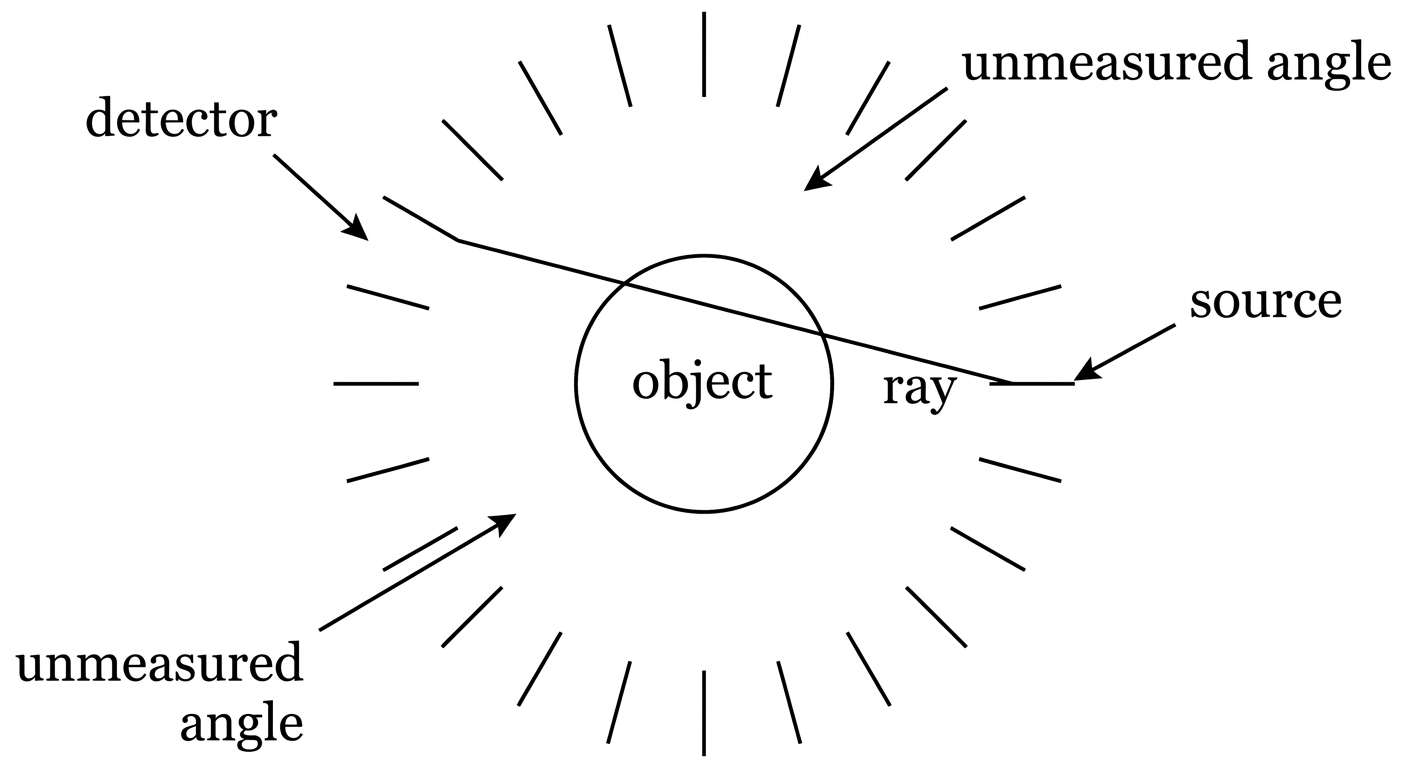
\includegraphics[width=0.92\textwidth]{fig_ct_geometry.png}
\caption{\textbf{Sparse-view acquisition geometry, as a two-panel schematic.} A source is drawn as a
filled triangle and its opposing detector as a thick bar, identified once by a legend rather than by
arrows aimed at the ring. Panel~(a): twelve source-detector pairs spaced all the way round the object,
with one ray drawn plainly through it --- every angle measured. Panel~(b): four pairs, at top, right,
bottom and left, and the hatched wedge is the angular range no view ever crosses --- most angles
missing. The contrast between the panels is the whole content, and it is the contrast
\eqref{eq:ch36-slice} turns into a null space: what is not sampled is not recovered. The plate shows
no phantom reconstruction, no Hounsfield value and no error figure; quantitative claims belong to the
text and its citations, not to this figure.}
\label{fig:vol3_ct}
\end{figure}

How the data fail matters as much as how sparse they are, and the two
arrangements of the next section attach to one failure each. Sparse-view
acquisition is a \emph{density} failure: the angular range is complete, the
samples inside it are too few, and adding views at finer spacing repairs the
defect in the limit. Limited-angle acquisition is a \emph{coverage} failure: an
arc is absent, no number of extra views inside the measured arc recovers it, and
the null space contains smooth anisotropic structure --- the kind of content a
prior is most willing to invent. One geometric fact governs both. The sinogram
is periodic in one coordinate and not the other: $\theta$ closes on itself
modulo the identification $p(\theta+\pi,-s) = p(\theta,s)$, while $s$ is a
finite interval across which nothing repeats. A spectral treatment of the
sinogram tensor must therefore choose which axis carries the Fourier structure,
and a multiplier applied along $s$ silently imposes a wraparound boundary
condition no patient satisfies. That choice, not the depth of the network, is
what separates a tomographic operator from a stock two-dimensional spectral
model.

% -----------------------------------------------------------------------------
\section{Two Operator-Learning Arrangements}
\label{sec:ch36-operators}
% -----------------------------------------------------------------------------

Two arrangements introduce continuous neural operators into this pipeline, and
the inherited record presents them as one family. They are not. The first
targets sparse-view data at \emph{several} sampling rates
\index{sparse-view CT}. It rests on two claims, and the property they buy
together is of exactly the kind Part~I's discretization-invariance machinery was
built to state. The first claim is a dual-domain design: the network acts in
sinogram space and in image space, where an artifact localized in one is spread
across the other \index{dual-domain reconstruction}. The second is that its
convolution kernels are parameterized as functions on the continuum and evaluated
on whatever grid the data arrive on, so that the parameters are decoupled from
the detector sampling density; the same parameterization is additionally made
equivariant to the rotations the tomographic geometry acts with, the rotational
structure the previous section located in the angle axis
\index{rotation equivariance}\index{resolution-agnostic operator!see also
discretization invariance}. The consequence is the property such a model is built
for: one trained network reconstructs data acquired at different angular and
detector rates without retraining. Whether it is \emph{accurate} at a rate it was
never trained on is the separate question Section~\ref{sec:ch36-metrics} returns
to, and the two shifts a device serving many protocols must actually survive ---
a change of dataset, a change of noise level --- are measured rather than granted
by the parameterization. Inference in this arrangement is an unrolled
cascade alternating sinogram-domain operator refinement, projection-data
consistency updates with $\mathcal{A} = \mathbf{M}\mathcal{R}$, and image-space
operator denoising. Displayed in the form such steps usually take, the
consistency update is
\begin{equation}
  \label{eq:ch36-consistency}
  u^{(j+1)} = u^{(j)} - \gamma_j\, \mathcal{A}^{*}\big(\mathcal{A} u^{(j)} - p_\delta\big), \qquad \mathcal{A} = \mathbf{M}\mathcal{R},
\end{equation}
with $p_\delta$ the measured noisy sinogram, $\mathcal{A}^*$ the adjoint of the
sampled forward operator, and $\gamma_j$ a step size; in the unrolled setting
$\gamma_j$ and the surrounding refinements are learned rather than chosen, and
the fixed projection becomes a learned operator applied a fixed number of
times \index{data-consistency projection}.

The second arrangement addresses the other defect: \emph{limited-angle}
tomography, in which an arc of the acquisition is simply absent
\index{limited-angle tomography}. Its posture is the opposite of an unrolled
cascade, and its substitution is a single one: a Fourier
neural operator (FNO)\index{Fourier neural operator (FNO)!in reconstruction} in
the sense of \cite{li2021fourier} is inserted into the filtering stage of FBP
itself, so the
analytic structure of \eqref{eq:ch36-fbp} is retained and the learned component
is confined to extrapolating the sinogram into the unmeasured angular region
before backprojection. The extrapolation is not free-form; it is constrained by
the \emph{moment conditions}, the family of identities
\begin{equation}
  \label{eq:ch36-moment}
  m_k(\theta) \;=\; \int_{\mathbb{R}} s^{k}\, p(\theta,s)\, ds \;=\; \int_{\mathbb{R}^2} f(x)\,\big(x_1\cos\theta + x_2\sin\theta\big)^{k}\, dx, \qquad k = 0,1,2,\ldots.
\end{equation}
The second equality is \eqref{eq:ch36-radon} tested against $s^k$. Its content is
that for data which are the projection of \emph{some} attenuation field, the
right-hand side is a homogeneous polynomial of degree $k$ in
$(\cos\theta,\sin\theta)$
\index{moment conditions (range conditions)!Helgason--Ludwig type}. Total mass,
center of mass, and the second moments of $f$ are read off $m_0$, $m_1$, $m_2$,
so an extrapolation preserving these low-order moments cannot add or relocate
mass: it stays inside the range of the continuous transform up to the order at
which the conditions are imposed. That is the whole content of the instruction
to enforce moment conditions, and it is why the arrangement is defensible on real
incomplete data rather than merely fitted to them. Two consequences follow from
keeping the analytic pieces analytic. The first is a cost accounting in the
console's own units: this arrangement inserts one learned completion of the
sinogram into a pipeline whose projection pass it does not touch, whereas an
unrolled cascade changes what the console has to run and must be priced from
scratch. Whether a learned filtering stage in fact executes at FBP's cost on a
given scanner is a measurement this book does not have, and it is not a
comparison the arrangement's structure settles. The second is that the residual
of \eqref{eq:ch36-consistency} remains available as a check on the completed
data: the extrapolated wedge can be reprojected and tested against the measured
rays without a reference image in hand, which is the check
Section~\ref{sec:ch36-metrics} returns to.

Table~\ref{tab:ch36-operators} sets the two side by side, and the row to read
is the fourth. The cascade's commitment is on sampling \emph{density}, precisely
the variable Part~I's definition of discretization invariance governs; the
learned filtering stage's is on angular \emph{coverage}, which is not a
discretization of anything but a property of the geometry, and no
resolution-agnostic parameterization removes it. The final row is the editorial
accounting: the inherited record attaches accuracy and runtime gains to specific
reconstructors, and this book carries none of them, because a margin is a
statement about the model it was measured on. The consequences for how such a
margin should be read are Section~\ref{sec:ch36-metrics}.

\begin{table}[htbp]
\centering
\small
\caption{\textbf{Two operator reconstructions, two defects.} The two arrangements of Section~\ref{sec:ch36-operators} as this book formulates them. The discretization row is this book's reading of what each arrangement commits to; the other rows state where the learning sits and what is left analytic. No accuracy or runtime figure is carried: the measurements in the inherited record belong to reconstructors this book does not name, and Section~\ref{sec:ch36-metrics} explains why a margin quoted against untuned filtered backprojection is not a margin against the classical recipe.}
\label{tab:ch36-operators}
\resizebox{\textwidth}{!}{%
\begin{tabular}{lll}
\toprule
 & \textbf{Unrolled cascade} & \textbf{Learned filtering stage} \\
\midrule
Defect addressed & Sparse view: too few angles, full arc & Limited angle: arc missing entirely \\
Where learning acts & Sinogram and image domains, alternated & Sinogram extrapolation inside FBP \\
What stays analytic & Projection $\mathbf{M}$, Radon $\mathcal{R}$ in \eqref{eq:ch36-consistency} & Ramp filter and backprojection $\mathcal{R}^*$ in \eqref{eq:ch36-fbp} \\
Discretization commitment & Detector and view density, deliberately removed & Angular range, deliberately retained \\
Figures certified here & None; multi-rate gains unmeasured & None; cost relative to FBP unmeasured \\
\bottomrule
\end{tabular}%
}
\end{table}

% -----------------------------------------------------------------------------
\section{Reported Accuracy, Error Accounting, and Failure Modes}
\label{sec:ch36-metrics}
% -----------------------------------------------------------------------------

Reconstructions of this kind are reported in three quantities, all of them
computed against a reference image $f$ --- a full-dose or simulated
reconstruction that the low-dose protocol being evaluated does not itself possess
--- on a display window with peak level $L$. With $u$ the reconstruction and
$\Omega$ the field of view,
\begin{equation}
  \label{eq:ch36-metrics}
  \begin{aligned}
    \mathrm{RMSE}(u,f) & = \Big( \tfrac{1}{|\Omega|}\int_{\Omega} \big(u(x)-f(x)\big)^{2}\,\mathrm{d}x \Big)^{1/2}, \\[2pt]
    \mathrm{PSNR}(u,f) & = 10\log_{10}\!\big( L^{2}/\mathrm{RMSE}(u,f)^{2} \big),
  \end{aligned}
\end{equation}
where the root-mean-square error (RMSE)\index{root-mean-square error (RMSE)} is
taken in Hounsfield units and the peak signal-to-noise ratio
(PSNR)\index{peak signal-to-noise ratio (PSNR)} is its logarithmic rescaling; the
third quantity, the structural similarity index measure
(SSIM)\index{structural similarity index measure (SSIM)}, compares local
luminance, contrast and structure between $u$ and $f$ over a sliding window. The
operating points the inherited record attaches to an abdominal and kidney CT
benchmark at $18$ projection views are not reproduced here. They were measured on
reconstructors this book does not name; a point on a curve and an average over
sampling rates are different objects, and the record mixed the two; and the
baseline they were quoted against is not the classical recipe but one
parameterization of it. That last defect is independent of which network sits on
the other side of the comparison. A baseline whose RMSE spans the whole
soft-tissue band marks itself as an FBP of the raw sparse data rather than a
tuned one: at $18$ views a console runs
an apodizing window and an object mask, each trading resolution for the very
streak suppression the comparison is meant to win, and the fair comparator at
low view count is a regularized iterative reconstruction. ``Outperforming
classical FBP'' is thus a statement about one parameterization of a method.

Of the three quantities in \eqref{eq:ch36-metrics}, only RMSE is interpretable
without further
convention. The Hounsfield unit (HU)\index{Hounsfield unit (HU)} is the
calibrated attenuation scale $\mathrm{HU}=1000(\mu-\mu_{\text{water}})/\mu_{\text{water}}$,
with air near $-1000$, water at $0$, and cortical bone well above
$+1000$. An RMSE of a few tens of HU is an absolute attenuation error of a few
percent of the water-to-bone span, and of the same order as the contrast between
a focal lesion and the parenchyma around it. The honest reading of an error at
that magnitude is less
flattering than a decibel figure sounds: the reconstruction is accurate to
within the contrast it must display --- a claim about detectability at the edge
of the range, not about recovery.
PSNR is a logarithm relative to the assumed peak $L$ of
\eqref{eq:ch36-metrics}, and the peak convention
--- window, level, clipping --- moves it by several dB at fixed error, so a dB
figure without its convention does not compare across papers.
SSIM rewards smoothness, so an over-smoothing network can
beat a sharper one while destroying the low-contrast features the dose reduction
existed to preserve, and it is full-reference: the ground truth a low-dose
protocol lacks is borrowed from a full-dose or simulated scan, itself a
reconstruction with its own kernel. Task-based evaluation --- lesion detection
scored by an observer study or a model observer --- is what a radiologist
consumes, and no reconstruction discussed here is verified against it in this
book
\index{task-based image quality assessment|textbf}.

Error accounting says why better metrics will not close that gap. Decompose the
reconstruction error orthogonally in $L^2(\mathbb{R}^2)$ against the null space of
the sampled operator:
\begin{equation}
  \label{eq:ch36-error}
  \hat f - f \;=\; \Pi_{\mathcal{N}(\mathcal{A})}\big(\hat f - f\big) \;+\; \big(I - \Pi_{\mathcal{N}(\mathcal{A})}\big)\big(\hat f - f\big),
\end{equation}
with $\hat f$ the reconstruction, $f$ the truth, $\mathcal{A}=\mathbf{M}\mathcal{R}$
as before, and $\Pi_{\mathcal{N}(\mathcal{A})}$ the orthogonal projector onto
$\mathcal{N}(\mathcal{A})$ \index{null space!of the sampled measurement
operator}\index{error decomposition!in tomographic reconstruction}. The identity
is the argument. A reconstruction exactly consistent with the measured data puts
all of its error in the first term, where the measurement at hand cannot find
it; that term is set by the learned prior, not by the physics.
Which term dominates is regime-dependent: at $18$ views the null-space term
governs and the image is prior-driven; at full sampling with low dose the second
governs, and what matters is noise propagation and the consistency residual in
\eqref{eq:ch36-consistency}. Across protocols a third error binds, outside
\eqref{eq:ch36-error} because that split holds the operator fixed: the
approximation and discretization error that attaches to the discretization-invariant
formulation \cite{kovachki2023neural}, bounded in this book as \eqref{eq:ch06-rate}
under a compactness hypothesis on the training support --- the discretization leg
of \eqref{eq:ch06-decomp} \cite{subedi2024controlling}. The
caveat of
Section~\ref{sec:ch06-zeroshot} bites harder here than anywhere in the book:
moving one model to a finer grid is resolution \emph{transfer}, not recovery of
detail the sampling destroyed, and in sparse-view acquisition that detail is
genuinely gone --- which is why the moment conditions of
\eqref{eq:ch36-moment} constrain the extrapolation rather than supply content.

Two verification consequences follow. Held-out error on the training
distribution scores a network on the prior it was trained to use, so the checks
that bite move the protocol: train at high view count and serve at low, train on
one dataset and test on another, inject sinogram noise and watch the image
metrics and the HU bias separate. The cheaper check needs no ground truth at all:
reproject the reconstruction with $\mathcal{A}$ and compare against the measured
$p_\delta$, so that a large residual becomes the refusal the deployed-surrogate
test of \chapref{ch:part2-production-deployment-and-high-throughput-} asks for
but cannot supply, needing held-out labels where this check does not
\index{verification!consistency check at inference}. The failure modes are then
predictable. Streak suppression and lesion restoration act on the same degrees
of freedom, so the boundary recovered in box~B of
Figure~\ref{fig:vol3_ct} is an inference, and the only defensible safety statement
about it is conditional on the training distribution. HU error is not cosmetic:
treatment-planning systems convert HU into electron density, so a bias of tens of
units propagates into whatever the next device computes. Data are the binding
constraint: paired low-dose and reference scans are expensive, and the reference
carries its own kernel. Clinical reconstruction software is also
regulated as a medical device, cleared against a predicate device's output --- a
harder comparison when the noise texture varies with the anatomy, since the two
images are then not two renderings of one measurement.
Prospective multi-center validation on diverse cohorts is the roadblock named in
\chapref{ch:part3-synthesis-matrix-and-real-world-deployment};
``resolution-agnostic'' describes a model's parameterization, not a waiver of
per-protocol verification \index{medical device
regulation!of reconstruction software}.

% -----------------------------------------------------------------------------
% Bridge to Chapter 3.7
% -----------------------------------------------------------------------------
\medskip
Every reconstruction above is an arrangement of two kinds of constraint. The
moment conditions \eqref{eq:ch36-moment} are hard in the strong sense: an
extrapolation that satisfies them does so whatever the weights happen to be,
because the admissible set is built into the computation rather than asked of
it. The projection step \eqref{eq:ch36-consistency} is hard in a weaker sense
easy to lose: $\mathcal{A}$ and $\mathcal{A}^*$ there are the analytic
operator and its adjoint, unlearned even where $\gamma_j$ is not.
The learned prior is soft: it holds in expectation, at a weight
chosen during training, and it is exactly where the null-space term of
\eqref{eq:ch36-error} lives. Stripped of tomography, that opposition is the
subject of \chapref{ch:part3-boundary-condition-enforcement-neural-oper}.
Classical solvers impose boundary data by construction --- Dirichlet conditions
carried by the test space $v \in H^1_0(\Omega)$ in the finite element method,
local flux balance across cell interfaces in the finite volume method,
boundary-conforming bases in a spectral discretization
--- whereas a neural operator's global convolution satisfies none of them by
default, and the field-of-view edge, the object's support, and the periodicity of
the angle axis are boundary conditions in disguise. The next chapter compares
the two remedies: a distance envelope that attains the
boundary value for every parameter vector, and a penalized boundary residual in
the loss. This chapter has priced that distinction from the other side. In
tomography the hard constraint costs one reprojection and the soft one carries
the entire error budget --- a ratio worth knowing before the choice is made for
a partial differential equation\index{boundary condition!hard versus soft
enforcement}.

% Chapter 3.7: Boundary Condition Enforcement: Neural Operators vs. Classical Solvers
% Part III of the book.
% STATUS: rewritten to book standard (Part III draft pass).

\chapter{Boundary Condition Enforcement: Neural Operators vs. Classical Solvers}
\label{ch:part3-boundary-condition-enforcement-neural-oper}
\label{sec:boundary_conditions}
% -----------------------------------------------------------------------------

A boundary condition is half of the physical statement, not a comment on it. In every application
of this part the trace of the solution on some surface carries either the physics or the
deliverable.
\index{boundary condition!enforcement regimes}
External aerodynamics is the plainest case: no-slip
\index{no-slip condition}
on the body is a Dirichlet condition on the velocity, and the reported quantities of
interest---drag and lift coefficients, surface pressure, wall shear stress (WSS)---are integrals
over the same surface (\chapref{ch:part3-external-aerodynamics-and-surface-flows}). In cardiac
electrophysiology the zero-flux condition through the endocardium and epicardium helps determine
whether a reentrant spiral wave persists, drifts, or annihilates
(\chapref{ch:part3-cardiac-electrophysiology-and-arrhythmia-d}). In a faulted aquifer the
load-bearing constraint sits inside the domain, on the impermeable caprock across which carbon
dioxide has no normal flux (\chapref{ch:part3-subsurface-multiphase-flow-and-carbon-stor}).
Global weather prediction supplies the exception that defines the rule: the horizontal domain is
the sphere, which has no boundary, while the vertical has a ground and a model lid, and what the
poles require is regularity rather than boundary data
(\chapref{ch:part3-global-weather-forecasting-and-climate-dyn}). Tomography has no boundary
condition at all but has the analogous object, the support of the attenuation field together with
the detector's sampling domain (\chapref{ch:part3-medical-imaging-and-tomographic-reconstruc}).

This chapter treats that structure in general, and it belongs between the application chapters
because the comparison the book has been building is sharpest at the boundary. A conforming
discretization cannot return a field that violates its boundary conditions, because the condition
is a property of the space being searched; no spectral, graph, or branch-and-trunk layer has that
property by construction. A trained operator reproduces boundary values when its labels carry them
and fails when they do not, and the resulting error is nearly invisible in an average norm while
decisive in a certified design loop. \chapref{ch:part3-the-multi-query-bottleneck-in-computationa}
established why the surrogate is worth building. Added here is an accounting of what is given up,
and of the three ways to buy it back: build the condition into the parameterization, add it to the
objective, or leave it to the data and measure the consequence.

Section~\ref{sec:ch37-classical} states the classical mechanisms and pins down what ``hard'' means.
Section~\ref{sec:ch37-operator} gives the two operator-side mechanisms and the
qualifications each carries, Section~\ref{sec:ch37-structural} collects the structural
routes---coordinate channels, lifting, parameterizations that satisfy the condition by
form---and their cost in regularity, geometry work, and guarantees, and Section~\ref{sec:ch37-ledger}
prices the mechanisms
against an elliptic stability estimate before separating what is proven from what is observed.

% -----------------------------------------------------------------------------
\section{Classical Numerical Paradigms (FEM, FVM, Spectral)}
\label{sec:ch37-classical}

The three workhorses of scientific computing enforce boundary conditions by one device, and the
device is not a penalty. In a conforming discretization the condition is imposed on the space from
which the numerical solution is drawn, so every member of that space---the exact discrete solution,
every Krylov or Newton iterate on the way to it, and every diagnostic read off them---satisfies it
by construction. Nothing is appended to an objective and no weight is tuned. The three variants
named in the section title are three realizations of that idea.

Consider the finite element method (FEM)
\index{finite element method (FEM)!essential boundary conditions}.
Trial and test spaces are chosen before any basis, quadrature, or solver appears; the Darcy problem
\eqref{eq:darcy} was put in that form as \eqref{eq:ch03-weakform}, with test space $H^1_0(\Omega)$,
the closure of $C_c^{\infty}(\Omega)$ in $H^1(\Omega)$ from
\chapref{ch:part1-function-spaces-duality-and-sobolev-regula}. For the Poisson model the statement
is
\begin{equation}
  \label{eq:ch37-fem-weak}
  \int_\Omega \nabla u \cdot \nabla v \, dx = \int_\Omega f v \, dx + \int_{\partial\Omega} g v \, ds
  \qquad \text{for all } v \in H^1(\Omega) \text{ with } v|_{\Gamma_D}=0,
\end{equation}
where $\Gamma_D$ is the part of $\partial\Omega$ carrying prescribed values and $g$ the prescribed
Neumann (traction) data on the complementary part $\Gamma_N$; the boundary integral is written over
all of $\partial\Omega$ and reduces to $\Gamma_N$, because the test function vanishes on $\Gamma_D$.
With $\Gamma_D=\partial\Omega$ the display collapses to the pure-Dirichlet form,
\eqref{eq:ch03-weakform} with $a\equiv1$; with $\Gamma_D=\varnothing$ it is the pure-Neumann
problem, which is
solvable only when $f$ and $g$ satisfy a compatibility condition and then only up to a constant.
Two facts about
\eqref{eq:ch37-fem-weak} are habitually collapsed into one. The Dirichlet condition carried by the
trial space is \emph{essential}: it is imposed, and it holds as an identity of the linear system,
which is why Poincar\'e's inequality \eqref{eq:ch02-poincare}, in its variant for functions
vanishing on a part of the boundary, makes the energy gradient a
norm \index{boundary condition!essential and natural}. The Neumann condition is \emph{natural}: it
enters as data in the right-hand functional and is satisfied only in the integrated sense against
test functions, so the prescribed flux is recovered from the discrete solution rather than built
into it~\cite{evans2010partial,quarteroni2008numerical}. The distinction matters because it
identifies which half of a boundary condition a change of representation preserves for free, and it
bounds the word ``exact'': a curved $\partial\Omega$ is replaced by straight or isoparametric
faces, the condition is imposed on that approximation, and the discrepancy is the standard geometric
error of the method \index{finite element method (FEM)!geometric approximation error}, removable
only by refinement and only where the boundary is smooth enough for the interpolation to converge.

The finite volume method (FVM) enforces a different property, local conservation, with the same
absence of a penalty. For a control volume $V_i$ with faces $f$, numerical flux $\mathbf{F}_f$, and
outward unit normal $\hat{\mathbf{n}}_f$,
\begin{equation}
  \label{eq:ch37-fvm-cons}
  \frac{\partial}{\partial t} \int_{V_i} u \, dx + \sum_{f \in \partial V_i} \mathbf{F}_f \cdot \hat{\mathbf{n}}_f = 0 .
\end{equation}
Boundary conditions enter by fixing the exterior, or ghost-cell, states from which the boundary-face
flux is computed \index{ghost cell}\index{finite volume method (FVM)!conservative update}. The scope of the guarantee deserves precision, since it is easy
to oversell. Summing \eqref{eq:ch37-fvm-cons} over all cells makes every interior face appear twice
with opposite normals, so the total mass in $\Omega$ changes only through the fluxes the boundary
model itself admits: there is no numerical leakage in the sense of a spurious source, and that holds
to the arithmetic precision of the update regardless of how accurate the flux formula is
\cite{leveque2002finite}\index{conservation!discrete versus learned}. An inconsistent boundary state
yields an exactly conserved wrong answer. The statement again presupposes a mesh with faces on
$\partial\Omega$.

Spectral methods apply the same idea with global bases
\index{spectral method!boundary-conforming basis}: Chebyshev or Legendre polynomials, or spherical
harmonics, whose individual terms can be chosen to satisfy the condition, so that no linear
combination of them can violate it. The Fourier case is the instructive limit, because there the
basis \emph{is} the boundary condition: periodicity on $\mathbb{T}^d$ is built into the trigonometric
system and no trace constraint is left to impose---the assumption behind Part~I's spectral theory
and behind \eqref{eq:fno_layer}. Operational numerical weather prediction (NWP) dynamical
cores such as the European Centre for Medium-Range Weather Forecasts (ECMWF) Integrated Forecasting
System (IFS) truncate a spherical-harmonic expansion horizontally: no lateral boundary, the
surface and the model top closing the vertical column
\index{numerical weather prediction (NWP)!spectral-transform dynamical core}. The cost is
geometry: a global basis conforms to a box, a sphere, or a mapped image of one, and anything else
takes substructuring or penalty machinery.

The lesson that transfers is narrower than it looks. Hard enforcement is free at run time and
expensive per geometry---meshing a new vehicle, generating boundary-layer prisms, re-deriving a
mapping for a new ventricle---and that per-geometry cost, not the linear solve, is what the
multi-query workflows of this part cannot afford
\index{mesh generation!as the recurring cost}. Classical schemes bind exactness to conformity;
operator learning drops the conforming mesh, and with it the source of the exactness.

% -----------------------------------------------------------------------------
\section{Boundary Enforcement in Neural Operators}
\label{sec:ch37-operator}

Neither mechanism below is needed because operators are inaccurate; both are needed because
operators are unconstrained. A generic layer is pointwise lifting and projection around a nonlocal
integral operator, \eqref{eq:no_composition}, and on a uniform grid the spectral specialization
\eqref{eq:fno_layer} makes every one of those operations equivariant to translations on
$\mathbb{T}^d$---the property the multiplier form \eqref{eq:ch05-multiplier} buys---so a network fed
only field values cannot tell a feature at $x$ from the same feature at $x+h$. Nothing in the
composition restricts the trace of the output, whose regularity is not assumed to exceed $L^2(\Omega)$,
where the trace is undefined.

The canonical benchmark makes the exposure concrete. Darcy flow on the unit square,
\eqref{eq:ch25-darcy}, carries homogeneous Dirichlet data while the Fourier neural operator (FNO)
lives naturally on $\mathbb{T}^2$: either the domain is treated as periodic and the mismatch with
$u|_{\partial\Omega}=0$ is absorbed into the learned map, or the field is odd-extended
\index{Darcy flow!boundary condition convention}\index{Fourier neural operator (FNO)!periodic domain and boundary}.
The two define different operators, and a specification silent about which was taken leaves the
dominant error term unnamed. In the DeepONet form \eqref{eq:ch04-deeponet} the same difficulty is one
line of algebra: the trace of $\sum_k b_k(a)t_k(y)$ vanishes for every input only if the trunk
functions cancel on $\partial\Omega$ across a whole family of coefficient vectors, cancellations
gradient descent has no reason to arrange
\index{DeepONet!trunk basis and boundary conditions}.

Absent such structure a trained network learns the boundary condition as a regularity of its labels.
Within the training family that works; outside it the claim is statistical, and three features make it
fragile. The boundary has codimension one: an order-one error confined to a single cell layer of
thickness $h$ on a unit square contributes only order $\sqrt{h}$ to the domain $L^2$ norm, so a
surrogate reported at a few percent relative $L^2$ error can be wrong by an order-one amount exactly
where the objective functional is evaluated
\index{error metric!codimension one of the boundary}. The most variable region of a solution field is
typically the one nearest the boundary, which is why the pointwise normalizers \eqref{eq:ch21-normalize}
find small variance exactly where a condition pins the value. And a change of geometry invalidates the
learned trace wholesale: a wall absent from the training family has no labels on it.

The two available mechanisms differ along one axis: where the constraint lives, in the
parameterization or in the objective.
\index{hard boundary condition!distance envelope}
The first, hard enforcement through a distance envelope, satisfies a homogeneous Dirichlet condition
$u|_{\partial\Omega}=0$ on an arbitrary domain by scaling the output with a continuous distance
function $d(x,\partial\Omega)$ and adding the inhomogeneous part separately,
\begin{equation}
  \label{eq:ch37-hard}
  \mathcal{G}_{\text{hard}}(a)(x) = g(x) + d(x, \partial\Omega) \cdot \mathcal{Q}(v_L(x)),
\end{equation}
where $\mathcal{Q}$ is the pointwise projection of \eqref{eq:no_composition}, applied to the final
latent field $v_L(x)$, so that the envelope multiplies the network's own output, and $g$ is a smooth
extension of the boundary data into $\Omega$. Since
$d(x,\partial\Omega)=0$ for all $x\in\partial\Omega$, the condition holds identically for every
parameter vector $\theta$. That is a one-line proof rather than an experiment, and it is the only
point in this chapter at which an operator architecture attains the classical guarantee. Its
preconditions are classical too: $g$ must exist with the regularity the problem asks for, which
requires the trace to be defined on the output space, i.e.\ $H^{s}(\Omega)$ with $s>1/2$, the
condition \chapref{ch:part1-physics-informed-operators-and-sobolev-reg} records for hard constraints
\index{trace operator}\index{lifting!of inhomogeneous boundary data}.
Three qualifications bound what the exactness is worth.

(i) It is exactness relative to whatever $\partial\Omega$ means in the implementation. The envelope
is evaluated at nodes, so the surface it vanishes on is the discrete boundary of the computing box,
not the body modeled; the residual geometric error is the same object that limits
\eqref{eq:ch37-fem-weak} on a curved boundary, only now it is silent. (ii) The construction
constrains values and nothing else. Where $d$ is differentiable its gradient has unit length and is
normal to $\partial\Omega$, so the normal derivative of the product on the boundary is, up to sign,
$\mathcal{Q}(v_L)$ itself: the flux is left entirely free. That is the correct division of labor for
a Dirichlet problem and no assistance at all for a Neumann, zero-flux, or no-penetration condition.
(iii) There is a regularity cost that
\chapref{ch:part1-discretization-invariance-and-continuum-li} is able to price. A distance function
is Lipschitz on $\overline{\Omega}$ and as smooth as $\partial\Omega$ near it, but loses
differentiability on the interior medial axis, the locus of points with more than one nearest
boundary point \index{signed distance function (SDF)}\index{medial axis!regularity of the distance function}---not an exotic object in the geometries of this part, since the mid-surface of a
ventricular wall, the centerline of a channel, and the interior of a layered aquifer all have one.
Multiplying by a Lipschitz envelope caps the Sobolev regularity of the product; feeding the distance
in as an input channel instead puts a non-periodic function on a periodic grid, jumping across the
wrap wherever the modeled boundary is not a face of the box, with regularity
$H^{1/2-\epsilon}$ for every $\epsilon>0$ and no better---the obstruction that chapter records for
non-periodic coordinate channels, and the reason the discretization rate in \eqref{eq:ch06-rate}
fails to reach $N^{-1}$.

The second mechanism is soft: a variational penalty on the boundary residual,
\begin{equation}
  \label{eq:ch37-soft}
  \mathcal{L}_{\text{boundary}}(\theta) = \lambda_{\text{bc}} \int_{\partial\Omega} |\mathcal{B}(\mathcal{G}_\theta(a)) - g|^2 \, ds,
\end{equation}
where $\mathcal{B}$ is whatever boundary operator the problem states---trace for Dirichlet, normal
flux for Neumann, both for no-slip---and $\lambda_{\text{bc}}$ is a weight. This is the boundary term
of the physics-informed objective \eqref{eq:ch07-bc-loss}, used by the Physics-Informed Neural
Operator (PINO) constructions of \chapref{ch:part1-physics-informed-operators-and-sobolev-reg},
specialized here to the $L^2$ surface norm, so the properties established there transfer: the weight
is dimensional, its usable size depends on the nondimensionalization chosen, and the surface integral
must be realized as a quadrature over a node set on $\partial\Omega$ at every training step
\index{Physics-Informed Neural Operator (PINO)!boundary term}\index{Neumann condition}.
The reported benefits of such training belong to the composite objective and are recorded there~\cite{li2021physics,raissi2019physics};
they are benchmark outcomes, and \eqref{eq:ch37-soft} alone buys no constraint. What the two
mechanisms do buy is priced in Section~\ref{sec:ch37-ledger}.

% -----------------------------------------------------------------------------
\section{Structural Routes: Coordinate Channels, Lifting, and Boundary-Condition-Invariant Parameterizations}
\label{sec:ch37-structural}

Between the two mechanisms sits a family of design choices, differing by which object is modified:
the input representation, the output representation, or the space of admissible outputs itself.

On the input side the cheapest intervention is an extra channel. The grid embedding of
\chapref{ch:part2-the-practitioner-s-paradigm-infinite-dimen} appends normalized coordinates to the
input; a distance-to-boundary channel, a signed distance function, an inside/outside mask, or a
boundary-curvature field are the same device with a physically meaningful scalar in place of $x_1$.
What it buys is a location: the network can condition its response on distance to the wall, so a
boundary layer becomes a function of a physical thickness rather than of a pixel count, and a mask
keeps the model from predicting into solid or void regions at all
\index{coordinate channels!distance to boundary}. What it does not buy is enforcement. The lifting
convolution mixes the channel into the hidden representation, exactly as
\chapref{ch:part2-fourier-neural-operators-fno-from-scratch} describes for the coordinate pair, and
the output trace stays unconstrained: the channel makes the right answer easier to fit and nothing
more.

On the output side, \eqref{eq:ch37-hard} is one instance of a lifting scheme---hand the network the
deviation from a field that already satisfies the condition, then add the field back. For a
grid-based model the envelope is applied after the projection; for DeepONet the same idea folds into
the trunk by replacing $t_k$ with $d\cdot\varphi_k$, so every term of \eqref{eq:ch04-deeponet} has
vanishing trace and exactness holds at every query coordinate for free. The scheme's exposure is the
extension $g$, which is a hypothesis about the boundary data: if the data in use are not well
approximated within the regularity class of the chosen extension, the surrogate inherits an
irreducible error equal to that mismatch, and the extension's smoothness caps the smoothness of the
output, hence the rate in \eqref{eq:ch06-rate}. The scheme has an implementation precondition as
well: it presupposes a distance function that can be evaluated, and on a high-dimensional manifold
evaluating one is the difficulty. Where it bites, practitioners use the penalty
\eqref{eq:ch37-soft} instead.

The third family is the one spectral methods already practice: parameterize the unknown so that
every element of the family satisfies the condition---a stream-function or divergence-free form for
incompressible velocity, a basis of functions vanishing on the boundary, a discretization of the
monodomain operator that admits no flux through the organ surface. In operator learning these remain
largely unbuilt, and their status is the analogue of choosing a conforming Galerkin space: exactness
by construction, and a construction redone whenever the geometry changes. The Fourier basis on the
torus is the single case where the construction is free and uniform---and the geometry it is
indifferent to is fixed at $[0,1]^d$, which is why the periodic benchmark family of
\chapref{ch:part2-canonical-pde-benchmarks-and-reference-wor} is at once cheap and silent about this
chapter's question.

Where geometry genuinely varies, graph-based architectures relocate the problem rather than solve it.
In the geometry-informed neural operator (GINO) the surface mesh \emph{is} the domain of the model:
points are lifted to a latent grid, the spectral work happens there, and the decode returns pressure
and WSS at surface vertices, where the quantities of interest live
\cite{li2023geometry}\index{Geometry-Informed Neural Operator (GINO)!surface as domain}. There is
then no exterior ghost cell to fill and no trace to impose from the network's standpoint---the model
is asked nothing about the field inside the body, and nothing about the velocity on the surface,
whose pressure and traction are all it returns. No-slip survives only as a regularity of the labels
on surface nodes, and nothing in the graph neural operator (GNO) kernel \eqref{eq:ch24-gno-kernel}
obliges a predicted wall traction to be consistent with a wall velocity of zero
\index{no-slip condition!in surface-mesh operators}. The geometry must still be encoded, and
\chapref{ch:part2-graph-neural-operators-gno-and-irregular-g} records the cost: a signed-distance and
coordinate-channel pipeline rebuilt for every new computer-aided design tessellation. The same
substitution appears at internal interfaces. A finite volume scheme puts faces on the caprock, and
conservation across them follows from the telescoping that made \eqref{eq:ch37-fvm-cons} exact; an
operator on a fixed grid sees a fault or layer boundary as a jump in a coefficient channel, and
conservation across it is a learned tendency with no discrete identity behind it
\index{interface condition!impermeable layer}.

% -----------------------------------------------------------------------------
\section{The Ledger: Error Accounting, Proven Claims, and Open Ones}
\label{sec:ch37-ledger}

What the two mechanisms of Section~\ref{sec:ch37-operator} buy can be priced, because the
needed estimate is standard. Let $a$ range over the uniformly elliptic class
$\mathcal{A}_{\text{adm}}$ of Assumption~\ref{ass:ellipticity}, let $v\in H^1(\Omega)$ be any trial
field with trace $\gamma(v)$ and residual $r_v\in H^{-1}(\Omega)$, and let
$u=\mathcal{G}_{\text{true}}(a)$. Lift the trace defect with a bounded right inverse of $\gamma$,
apply the coercivity of \eqref{eq:ch03-coercive} to the remainder, and
\begin{equation}
  \label{eq:ch37-trace-stab}
  \big\|v-\mathcal{G}_{\text{true}}(a)\big\|_{H^{1}(\Omega)}
  \;\le\; C\left(\frac{1}{a_{\min}}\,\|r_v\|_{H^{-1}(\Omega)}
  + \big\|\gamma(v)-g\big\|_{H^{1/2}(\partial\Omega)}\right),
\end{equation}
with $C$ depending on $\Omega$ and on the extension but not on $v$
\cite{evans2010partial,quarteroni2008numerical}\index{elliptic stability estimate}.
The a priori estimate \eqref{eq:ch07-apriori} of
\chapref{ch:part1-physics-informed-operators-and-sobolev-reg} is the case in which the second term
is absent, because there $v$ already has the correct trace. Equation \eqref{eq:ch37-trace-stab} says
more
than that boundary errors add to the total: the boundary enters as a term no amount of residual
minimization removes, measured in $H^{1/2}(\partial\Omega)$, a norm strictly stronger than the
$L^2(\partial\Omega)$ norm \eqref{eq:ch37-soft} shrinks---control in the former would take a
bound on a fractional tangential derivative of the trace defect, which the penalty does not attempt.
The envelope \eqref{eq:ch37-hard} is exactly the device that zeroes the term by construction,
leaving only the question of how small the residual is;
raising $\lambda_{\text{bc}}$ instead trades the boundary term against the data term, with the
recognizable symptom of a small measured boundary residual alongside a field wrong near the
wall. The estimate controls an $H^1$ error while the loss reports a relative $L^2$ one, the second
instance after \eqref{eq:ch31-functional} of a minimized metric and a certified metric that differ.

Table~\ref{tab:ch37-enforcement} arranges the six regimes along the axes that have mattered: what the
constraint is a property of, whether it holds exactly, what it costs, how it fails. The
conclusion is the third column read against the fourth. Exactness is relative to a discretized
object in every row where it appears, the three classical rows no less than the envelope row, and
each classical row buys it with an object tied to the domain---a conforming mesh, a flux stencil
on the faces, a basis for the specific geometry. The envelope row is exact by the same one-line
argument but for values only, on the nodes at which $d$ vanishes; the last two rows are not exact
at all. What the three operator rows share is nothing spent per query.

\begin{table}[htbp]
\centering
\small
\caption{Where a boundary condition can live: six enforcement regimes compared.}
\label{tab:ch37-enforcement}
\begin{tabularx}{\textwidth}{@{}>{\raggedright\arraybackslash}p{0.14\textwidth}%
  >{\raggedright\arraybackslash}p{0.16\textwidth}%
  >{\raggedright\arraybackslash}p{0.13\textwidth}%
  >{\raggedright\arraybackslash}p{0.16\textwidth}%
  >{\raggedright\arraybackslash}X@{}}
\toprule
\textbf{Regime} & \textbf{Condition lives in} & \textbf{Exact?} & \textbf{Marginal cost} & \textbf{Dominant failure mode} \\
\midrule
Conforming FEM & trial and test spaces & on the discrete space & mesh per geometry & curved-boundary geometry error \\
FVM with ghost cells & boundary-face flux & conserved averages & ghost-layer construction & non-conforming interfaces \\
Spectral & basis functions & for the modeled condition & basis tied to domain & nonsmooth or moving boundaries \\
Operator plus envelope & output parameterization & on the sampled $\partial\Omega$ & distance evaluation at setup & value-type conditions only \\
Operator plus penalty & objective function & no & boundary quadrature per step & norm mismatch and weight tuning \\
Operator plus labels & training distribution & no & nothing at inference & new geometry or new loading \\
\bottomrule
\end{tabularx}
\end{table}

Sort the remaining claims by status. Proven: the exactness of
\eqref{eq:ch37-hard} with respect to the set on which $d$ is evaluated; the estimate
\eqref{eq:ch37-trace-stab} under Assumption~\ref{ass:ellipticity} with boundary regularity on
$\Omega$; and the disappearance of the question on $\mathbb{T}^d$ and $\mathbb{S}^2$, where
\eqref{eq:ch07-bc-loss} has no surface to integrate over. Observed: that adding
\eqref{eq:ch37-soft} lowers the measured boundary residual, that composite physics-informed training
reduces label requirements and improves behavior above the training resolution~\cite{li2021physics},
and that geometry channels let one trained surface-mesh operator serve the nearby shapes of
\chapref{ch:part3-external-aerodynamics-and-surface-flows}. Not established
anywhere in this book: a theorem that a trained operator satisfies a boundary condition
to a stated tolerance, on a stated class of domains, in a norm where the trace is defined
\index{universal approximation!boundary conditions outside the norm}.
That gap is structural rather than merely unproved. The universality
bound \eqref{eq:ch04-unif-bound} is an $L^2(\Omega)$ estimate, and the trace operator is not a
continuous functional of $L^2(\Omega)$, so nothing prevents a sequence Cauchy in that norm from
violating the condition. Approximation theory and boundary analysis live in different
topologies, which is why exactness in operator learning must be engineered into the architecture, as
in \eqref{eq:ch37-hard}, rather than inherited from a density result.

Two consequences follow, both constraints on practice rather than on style. The first is
diagnostic: a surrogate whose objective lives on the boundary should be scored by the boundary
defect itself, in a norm that can be named, on held-out geometries and loadings. A relative
$L^2$ number on the training family is not evidence about the trace, and the near-zero-variance
locations of \eqref{eq:ch21-normalize} should be checked rather than tolerated, since they mark where
the condition is imposed. The second is institutional. An auditor of a classical computation
inspects a constraint space: the boundary condition is an enumerable property of the discretization,
exactly as the flux stencil of \eqref{eq:ch37-fvm-cons} is auditable. A
learned trace is a statistical claim about a label distribution, and the labels nearest the boundary
are the costliest to generate, because boundary-layer resolution sets the size of the whole mesh. The
region that matters most is where the data are thinnest---the regime the penalty
\eqref{eq:ch37-soft} was written for, and the one in which it is least verifiable
\index{certification!auditable constraint spaces}\index{data availability!boundary labels}.

% -----------------------------------------------------------------------------

Boundary conditions are the clearest instance of a pattern this part has met five times under five
names: a property that a conforming discretization carries by construction becomes, in a learned
operator, either a term to be traded off in an objective or a regularity of the data to be tested
for. The pattern is not confined to the trace. Conservation of mass, momentum, and energy fails in
the same silent way, and so does reliability outside the training distribution, where a classical
solver diverges, violates a time-step restriction, or refuses to converge while a network returns a
smooth, plausible, wrong field. \chapref{ch:part3-synthesis-matrix-and-real-world-deployment}
assembles these into a single cross-domain ledger---the five application chapters with the cost
ratio each row can form and the two rows that cannot, their fidelity metrics, and the rigorous
statement Part~I supplies---and then takes up five roadblocks between a published surrogate and a
deployed one: error estimation without a reference solver, exact conservation, the price of labels,
distribution shift, and clinical clearance. This chapter supplies the template for that synthesis: for each guarantee, ask
which object carries it, whether it is exact, what it costs, and what would have to be measured to
believe it.

% Chapter 3.8: Synthesis Matrix and Real-World Deployment Roadblocks
% Part III of the book.

\chapter{Synthesis Matrix and Real-World Deployment Roadblocks}
\label{ch:part3-synthesis-matrix-and-real-world-deployment}
\label{sec:synthesis}
\index{synthesis matrix|textbf}\index{deployment roadblocks|textbf}
% -----------------------------------------------------------------------------

The five application chapters of this part each replaced one solver with one surrogate, and
the ledger format this Part uses was meant to report two numbers for each: a ratio of wall-clock times and an
error against a reference field. Three of the five get both; the cardiac and tomography rows
carry neither a time ratio nor a measured field error, and the matrix says so. Those
numbers are defensible one at a time; taken together --- the way a design office or a clinic must
take them --- they are not comparable. The aerodynamic multiplier was formed
against a volume discretization of computational fluid dynamics (CFD) on a graphics processing
unit (GPU); the reservoir multiplier against an implicit finite difference simulator on a
central processing unit (CPU); the atmospheric multiplier against the spectral-transform
dynamics of the European Centre for Medium-Range Weather Forecasts (ECMWF) Integrated
Forecasting System (IFS); and in the tomographic row the comparison is not a timing but
a reconstruction quality at fixed radiation dose.\index{speedup factor!provenance of} A
synthesis records provenance before it records figures.
Table~\ref{tab:synthesis_matrix} does that, and adds the column the inherited accounting
leaves out:
which rigorous statement, if any, Part~I supplies for the architecture in the row.

The rest of the chapter concerns what a multiplier does not price. Every application here
was chosen because the query count $Q$ of \eqref{eq:ch01-cost-bookkeeping} --- $M$ as Part~I writes it --- is large, so the
amortization argument of
\chapref{ch:part1-introduction-the-paradigm-shift-to-infinit} holds; deployment is governed
by obstacles that argument does not reach. A certifier cannot run the reference solver on
the field being decided upon, so a reported error is anchored to a machine no longer in the
loop. A conservation law that a finite volume method (FVM) satisfies cell by cell is
satisfied by a trained network only on average. The labels that made the surrogate possible
were themselves solver runs, and that cost recurs with every retraining. A guarantee stated
over a compact subset of the training measure --- the hypothesis
Assumption~\ref{ass:ch09-compact} makes explicit --- licenses nothing about the geometry,
aquifer, pacing protocol, or scanner that arrives next.

Prerequisites are the book's: the error split \eqref{eq:ch01-error-split} in ledger
form \eqref{eq:ch06-decomp}, the architecture comparison of
Tables~\ref{tab:comparison} and~\ref{tab:ch8-ledger}, the deployment budget
\eqref{eq:ch27-budget}, and the five application chapters. Section~\ref{sec:ch38-matrix}
builds the matrix; Section~\ref{sec:ch38-columns} reads its columns against the arithmetic
that produced them;
Sections~\ref{sec:ch38-roadblocks} and~\ref{sec:ch38-data-shift} state the obstacles, each
with the estimate that makes it precise rather than rhetorical; Section~\ref{sec:ch38-closing}
returns to the question the book opened with and hands off to the back matter. No new
measurement, architecture, or theorem appears here; a closing chapter's value is that its
claims are already in print and can be held against one another.

% -----------------------------------------------------------------------------
\section{The Synthesis Matrix and What Its Columns Mean}
\label{sec:ch38-matrix}
% -----------------------------------------------------------------------------

Table~\ref{tab:synthesis_matrix} is ordered by application rather than by architecture,
because the domain fixes the equation, the mesh, the metric, and the reviewer. Each row is
the version of the multi-query surrogate problem \eqref{eq:ch01-solution-operator} that its
chapter posed: the Reynolds-averaged Navier--Stokes (RANS) equations for a rigid body in a
free stream, the hydrostatic primitive equations on a rotating sphere, two-phase Darcy flow
in a heterogeneous aquifer, the monodomain reaction--diffusion system on a patient-specific
ventricle, and the inverse Radon transform under angular
undersampling.\index{Darcy flow!two-phase}\index{monodomain equation}\index{Radon transform!inverse problem}\index{Reynolds-averaged Navier--Stokes (RANS) equations}\index{hydrostatic primitive equations}
The five rows are served by five architectures: the geometry-informed neural operator (GINO)
\cite{li2023geometry}, FourCastNet \cite{pathak2022fourcastnet} built on the adaptive Fourier
neural operator (AFNO), the U-Net-enhanced Fourier neural operator (U-FNO)
\cite{wen2022ufno}, the physics-informed neural operator (PINO) \cite{li2021physics}
applied to the monodomain system with an Aliev--Panfilov ionic gate
\cite{aliev1996simple}, and, in the tomographic row, a reconstruction built on the
Fourier neural operator architecture \cite{li2021fourier} as its layer --- the cite
names the layer, no published reconstruction system --- arranged either as an unrolled data-consistency
cascade or as a learned filtering stage inside filtered backprojection (FBP). The first
three are named models with published evaluations; the last two are formulations this
book's own chapters build rather than released networks, which is why their rows are
scored on quantities rather than on a published model's figures. Those quantities are the
drag coefficient $C_d$, the anomaly
correlation coefficient (ACC), the plume-restricted saturation mean-absolute error and the
relative pressure-buildup error, and the
image-quality measures defined in \eqref{eq:ch36-metrics}: peak signal-to-noise ratio
(PSNR), structural similarity index measure (SSIM), and root-mean-square error (RMSE) in
Hounsfield units (HU).

\begin{table}[t]
\centering
\footnotesize
\caption{\textbf{Synthesis matrix: application, governing system, architecture, cost ratio as formed, fidelity as reported, and the rigorous statement Part~I supplies.} Each of the three printed ratios has a different provenance: the aerodynamic row prints the cost--accuracy ratio reported by \cite{li2023geometry}; the weather row divides the study's sub-two-second surrogate latency, carried here as $1.8$\,s, by a $120$-minute per-member IFS figure this Part attributes (the study times whole ensembles: $82$\,min of wall-clock for a $15$-day, $51$-member run, Table~\ref{tab:benchmarks_hardware}); the carbon-storage row divides the $10$\,min average solve reported by \cite{wen2022ufno} by a query cost of $0.02$\,s --- the published $0.01$\,s per-field time doubled, because saturation and pressure are returned by two networks, as
\chapref{ch:part3-subsurface-multiphase-flow-and-carbon-stor} records. Every ratio is in essence a hardware-bound system comparison rather than an algorithmic one. Where no published pair of timings exists the ratio cell says so instead of printing a multiplier; a fidelity cell carries a measured claim only where a published study states one, and otherwise records this book's own accounting in the quantities its chapter defines. The final column uses the convention of Table~\ref{tab:ch8-ledger}: ``none here'' records that this book develops or cites no theorem for that architecture, not that the literature has no result.}
\label{tab:synthesis_matrix}
\begin{tabularx}{\textwidth}{@{}l >{\raggedright\arraybackslash}X l l >{\raggedright\arraybackslash}X >{\raggedright\arraybackslash}X@{}}
\toprule
\textbf{Domain} & \textbf{Governing system} & \textbf{Operator} & \textbf{Cost ratio} & \textbf{Fidelity as reported} & \textbf{Guarantee in Part~I} \\
\midrule
Aerodynamics
& steady incompressible RANS
& GINO \cite{li2023geometry}
& $2.6\times10^{4}$
& $C_d$ within $3\%$ at the reported cost ratio
& none here: neither graph stage nor latent grid proved
\\
\addlinespace
Global weather
& hydrostatic primitive equations on $\mathbb{S}^{2}$
& AFNO \cite{pathak2022fourcastnet}
& $4\times10^{3}$
& parity with IFS to day~3; $\mathrm{ACC}>0.6$ for TCWV beyond day~8
& none here: the rate theorem holds on the torus
\\
\addlinespace
Carbon storage
& two-phase Darcy flow, $S_w+S_g=1$
& U-FNO \cite{wen2022ufno}
& $3\times10^{4}$
& plume saturation MAE $1.6\%$, pressure error $0.68\%$
& truncation tail at a front, \eqref{eq:ch09-jump-tail}
\\
\addlinespace
Cardiac
& mono\-domain reaction--diffusion, anisotropic $\mathbf{D}(x)$
& PINO \cite{li2021physics}
& not reported
& no measured field error here; residual term \eqref{eq:ch07-pde-loss} only
& no parabolic analogue of \eqref{eq:ch07-apriori}
\\
\addlinespace
Tomography
& inverse Radon transform, angularly undersampled
& FNO-class, \chapref{ch:part3-medical-imaging-and-tomographic-reconstruc}
& not established
& no operating point carried; metric conventions \eqref{eq:ch36-metrics}
& none here: no stability constant for the inverse
\\
\bottomrule
\end{tabularx}
\end{table}

Read the cost column first: it is where a synthesis is sloppiest. Each printed
entry is either the aerodynamic cost--accuracy ratio, a published latency divided by
a baseline this Part attributes, or a published solve time divided by a per-field query
cost doubled by this Part's own two-network accounting --- the
provenances this matrix's own caption lays out, of which Table~\ref{tab:benchmarks_hardware}'s caption shows two and adds a further kind, book-assembled estimates. The
baseline each entry is priced against is a choice rather than a
fact. The baselines are recoverable from this part's own chapters: an OpenFOAM-class finite
volume solve for aerodynamics, an Eclipse-class implicit finite difference simulator for the
reservoir, openCARP finite elements for the cardiac row, the IFS for the atmosphere, and FBP
for tomography. The first of those names is already doing work the aerodynamic row's multiplier cannot support. The
$2.6\times10^{4}$ of the aerodynamic row is the cost--accuracy ratio at $3\%$ drag error
reported by \cite{li2023geometry}, formed against the study's own GPU-accelerated
volume-CFD solve --- the multi-core, two-V100 label-generation configuration of
\chapref{ch:part3-external-aerodynamics-and-surface-flows}, whose wall-clock time the study
does not pair with the ratio --- rather than against the CPU alternative quoted in that
chapter: $15$--$45$ minutes on a many-core node, itself flagged there as an
order-of-magnitude pairing this Part inherits, not a time the study reports for that
configuration; price the same GINO surrogate against that alternative and the multiplier
changes again. Neither quotient describes an algorithm alone: the
printed one pits a multi-GPU solve against a single-GPU evaluation, the alternative an
accelerator against a CPU cluster.\index{wall-clock ratio!choice of baseline}
The two cells this part's inherited ledger filled with $1{,}500\times$ and $100\times$
are entered here as unreported or unestablished: neither is traceable to a pair of timings over the
baseline its row names. The cardiac row carries no multiplier because the comparison
there is against a fine-mesh finite element solve whose cost this book does not price;
the tomographic row carries none because what is bought there is image quality at a
dose rather than time, and the reconstruction's expense is reckoned in reprojection
passes \eqref{eq:ch36-consistency}, not in seconds saved. Claims of parity with FBP's
runtime, or of a wide margin over other learned reconstructions, would be claims about
particular reconstructors, and this book makes none. An unreconstructable number in a table is how an
unsupported figure acquires a citation, and a synthesis is where the circulation stops.

% -----------------------------------------------------------------------------
\section{The Cost Column's Second Reading, Fidelity, and the Guarantee Column}
\label{sec:ch38-columns}
% -----------------------------------------------------------------------------

The cost column has a second reading. Expand the training cost into what it is --- solver runs
plus an optimization --- and the crossover query count of
\eqref{eq:ch01-cost-bookkeeping} becomes
\begin{equation}
  C_{\mathrm{sur}}(Q)
  \;=\;
  \underbrace{n_{\mathrm{lab}}\,c_{\mathrm{sim}}(N_{\mathrm{lab}}) + c_{\mathrm{opt}}}_{c_{\mathrm{train}}}
  + Q\,c_{\mathrm{eval}}(N),
  \qquad
  Q^{\star}
  \;=\;
  \frac{n_{\mathrm{lab}}\,c_{\mathrm{sim}}(N_{\mathrm{lab}}) + c_{\mathrm{opt}}}
       {c_{\mathrm{sim}}(N) - c_{\mathrm{eval}}(N)}.
  \label{eq:ch38-crossover}
\end{equation}
\index{crossover query count}
Equation \eqref{eq:ch38-crossover} is arithmetic; its consequence is a design rule. Where
$c_{\mathrm{eval}}(N)<c_{\mathrm{sim}}(N)$ and the labels were generated on a grid at least
as fine as the one served, $c_{\mathrm{sim}}(N_{\mathrm{lab}})\ge c_{\mathrm{sim}}(N)$ pushes
$Q^{\star}$ above the number of labeled solves $n_{\mathrm{lab}}$. A surrogate must answer
more fields than it was trained on before it costs less than the solver it replaced, and
labeling more finely than one serves raises the threshold without any change in the network.
That is why the five rows were worth building. Sampling a permeability or stiffness field by
Markov chain Monte Carlo (MCMC) is stated in
\chapref{ch:part3-the-multi-query-bottleneck-in-computationa} to want $10^{5}$--$10^{7}$
forward evaluations; a fifty-member atmospheric ensemble run twice daily is $36{,}500$ solves
in a year; an ablation plan is queried per candidate lesion under a latency no tetrahedral
solve meets. A single verification run should by contrast stay with a classical
solver, the qualification attached to \eqref{eq:ch01-cost-bookkeeping} in
\chapref{ch:part1-introduction-the-paradigm-shift-to-infinit}. The tomographic row differs in
kind: the operator is bought for image quality at lower dose rather than for wall-clock, and
the two defects it is bought against are not interchangeable. Sparse-view acquisition leaves
the angular arc complete with too few samples inside it, so one trained model may be asked
to serve several projection sampling rates; the limited-angle case removes an arc of the
acquisition entirely, and no density of sampling inside what remains recovers it.
\chapref{ch:part3-medical-imaging-and-tomographic-reconstruc} separates the two
arrangements along exactly that line. The gain figures an earlier version of this table
carried --- a margin at $18$ views, and an average margin over sampling rates measured
against convolutional baselines --- are dropped rather than restated: they were measured on
reconstructors this book does not name, and a point on a curve and an average over rates
are in any case different objects, which is why neither was convertible into the other.

The fidelity column asks for the same skepticism. Every metric printed
there is computable, which is why it was reported; none is the quantity a decision reads. A
$3\%$ error in $C_d$ is an integral over the surface, constraining neither the separation
location nor the wall shear stress (WSS) a drag-reduction change actually moves. The ACC is a
spatial correlation of two fields at one lead time, and \eqref{eq:ch09-weak} is this book's
reason for refusing to extrapolate it to the long-horizon statistics a climate application
consumes. A $1.6\%$ mean absolute saturation error inside the plume says nothing about where the
$\mathrm{CO}_2$ front sits or how much flux crosses the caprock, and the Gibbs analysis
around \eqref{eq:ch09-gibbs} explains why the number stays quiet: under a volume
average, whether in $L^2$ or in $L^1$, an error of fixed height on
a set of vanishing measure costs little in either average and a great deal in a permit. PSNR, SSIM,
and RMSE in HU \eqref{eq:ch36-metrics} are the most decision-adjacent of the five, being defined against a reference
reconstruction a radiologist accepts --- a reference that exists in the evaluation and not in
the clinic, where only the undersampled sinogram is
available.\index{fidelity metrics!as proxies for decisions}\index{tomography!sparse-view reconstruction}\index{aerodynamics!surface quantities not priced by drag error}\index{weather forecasting!skill over long horizons}

The last column is the one this book can sign. None of the five architectures above
carries a convergence theorem proved for it as used: Table~\ref{tab:ch8-ledger} gives GINO a
row and no theorem; the spectral layer behind FourCastNet is not the
translation-invariant multiplier of Theorem~\ref{thm:fno_convergence}, whose hypotheses live
on the torus; U-FNO contributes exactly the multi-scale content that rate does not price, and
\eqref{eq:ch09-jump-tail} shows what a front costs it; a reconstruction whose kernels are
parameterized on the continuum decouples its weights from the detector sampling density but
inherits no modulus of continuity for an undersampled inverse problem; and the arrangement
that keeps the analytic ramp and backprojection \eqref{eq:ch36-fbp} intact leaves the learned
part to extrapolate the missing angular wedge, for which this book supplies no
analysis.\index{Geometry-Informed Neural Operator (GINO)!in deployment}\index{adaptive Fourier neural operator (AFNO)}\index{U-Net-enhanced Fourier neural operator (U-FNO)!multi-scale content}\index{tomography!operator-learning reconstruction}\index{Physics-Informed Neural Operator (PINO)!cardiac application}
PINO is the one row with a theorem adjacent to it, and the adjacency is conditional: the
residual-to-error implication \eqref{eq:ch07-apriori} is proved there for a coercive
divergence-form problem whose trial field already has the correct trace, and no parabolic
counterpart is derived in this book for the monodomain system with its nonlinear ionic
current. The matrix thus records an exchange rate of five to one: real-time and lower-dose
answers, purchased with guarantees never attached to the purchased object.

% -----------------------------------------------------------------------------
\section{Translational Roadblocks to Production Deployment}
\label{sec:ch38-roadblocks}
% -----------------------------------------------------------------------------

The first obstacle is the one the ratio conceals: error estimation without a reference
solver. In the classical workflow a reviewer asks for a residual, a refinement study, or
both, because the solver is available and accuracy is purchasable at query
time --- the point \chapref{ch:part2-production-deployment-and-high-throughput-} makes against
its own speedup table. A deployed surrogate has no such dial: mode counts, width, and depth
are frozen in the archive of Implementation Pattern~\ref{imp:ch27-artifact}, so more compute
per query buys no accuracy. The principled substitute is a stability estimate, bounding the
error in the functional actually decided upon by the residual the surrogate's own output
produces:
\begin{equation}
  \big|J(u)-J(v)\big|
  \;\le\;
  L_J\,\big\|v-u\big\|_{\mathcal{U}}
  \;\le\;
  L_J\,C_{\mathrm{st}}\,\big\|\mathcal{N}(v;a)\big\|_{X^{*}(\Omega)},
  \qquad v = \mathcal{G}_{\theta}(a),
  \label{eq:ch38-residual}
\end{equation}
\index{error estimation!without a reference solver}\index{certification of learned surrogates}
Here $J$ is a functional on the output space $\mathcal{U}$, Lipschitz with constant $L_J$;
$\mathcal{N}(\,\cdot\,;a)$ is the residual operator of \eqref{eq:ch07-pde-loss}; $X^{*}(\Omega)$
is the dual test space measuring the weak residual; $u$ is the exact state; and
$C_{\mathrm{st}}$ is the stability constant of the underlying a priori estimate --- for Darcy
flow under the uniform ellipticity of Assumption~\ref{ass:ellipticity},
$C_{\mathrm{st}}=1/a_{\min}$ in the energy norm. Equation \eqref{eq:ch38-residual} is the
deployment form of \eqref{eq:ch07-apriori} and inherits its conditions: the trial field must
carry the correct trace, coercivity or an equivalent inf-sup condition must hold, and the
bound degrades as the ellipticity constant does. Read against the matrix, that machinery
exists in model form for at most one row --- the elliptic Darcy parent of the subsurface
problem --- and for none of the five as deployed. It has one further merit and one further
limit: the residual in \eqref{eq:ch38-residual} is computable at inference from the output
and the equation alone, with no label required, but its cost and its fidelity depend on being
able to differentiate the surrogate's output field --- exactly on the uniform periodic grids
of \chapref{ch:part2-fourier-neural-operators-fno-from-scratch}, approximately and at added
expense on the surface stages of \chapref{ch:part3-external-aerodynamics-and-surface-flows}. Where the estimate is
unavailable, the substitute is a schedule rather than a theorem: run the reference
solver on a randomly selected fraction of queries. That returns the audit to
\eqref{eq:ch38-crossover} as a term $Q_{\mathrm{audit}}\,c_{\mathrm{sim}}(N)$ and preserves
the surrogate's advantage exactly while $Q_{\mathrm{audit}}\ll Q$. Certification by sampling
is slower than inference and quicker than hope.

The second obstacle is conservation. Certifiers ask for guaranteed balance of mass,
momentum, and energy; an $L^2$-trained network delivers a bound on a global quantity and
nothing more. Let $\mathcal{T}(w)=\int_{\Omega}w\,\mathrm{d}x$ be the conserved total of a balance law
with no flux through $\partial\Omega$. H{\"o}lder's inequality converts the training error
into a defect estimate,
\begin{equation}
  \Delta_{\mathcal{T}}(v,u)
  \;:=\;
  \frac{\big|\mathcal{T}(v)-\mathcal{T}(u)\big|}{\big|\mathcal{T}(u)\big|}
  \;\le\;
  \frac{1}{\big|\mathcal{T}(u)\big|}\int_{\Omega}\!\big|v-u\big|\,\mathrm{d}x
  \;\le\;
  \frac{|\Omega|^{1/2}}{\big|\mathcal{T}(u)\big|}\,\big\|v-u\big\|_{L^{2}(\Omega)}.
  \label{eq:ch38-defect}
\end{equation}
\index{conservation laws!guarantees for learned surrogates}
The two inequalities in \eqref{eq:ch38-defect} are the global case of a family: test the same
argument against the indicator of a control volume rather than of $\Omega$ and it bounds that
cell's defect, which is the local form an FVM forecloses by construction, as
\chapref{ch:part3-boundary-condition-enforcement-neural-oper} develops. A small aggregate
defect is therefore entirely compatible with large cancelling imbalances between neighboring
cells. The
normalization itself deserves caution: $\Delta_{\mathcal{T}}$ is meaningless for a conserved quantity
whose net value vanishes --- circulation, net charge, the integral of a vorticity anomaly --- and
must then be measured against $\int_{\Omega}|u|\,\mathrm{d}x$ instead. The surrogate compounds
the difficulty by emitting states rather than the interface fluxes
$\mathbf{F}\cdot\hat{\mathbf{n}}$ a balance would be audited against, so the cell-wise defect
cannot be read from its output without a separate flux reconstruction. Imposing the balance by
construction is the right shape of answer and this book does not supply one: the
distance-envelope device of the chapter just cited enforces a trace, not a divergence
identity. What remains is weaker and should be reported as such --- penalize the balance
residual in the objective, in the spirit of the soft penalty \eqref{eq:ch07-bc-loss}, and
release on measured $\Delta_{\mathcal{T}}$ and its cell-wise analogue alongside the acceptance metric
Implementation Pattern~\ref{imp:ch27-artifact} requires the artifact to carry.

The third obstacle is the price of the labels, which \eqref{eq:ch38-crossover} places inside
$c_{\mathrm{train}}$ rather than outside the analysis. Supervised training needs paired fields, produced by the solver the
surrogate is meant to retire, at a resolution fine enough for the budget
\eqref{eq:ch27-budget} to certify against; retraining on the same labels does not shrink the
discretization term of that budget, and storing a three-dimensional field times a long
trajectory times hundreds of realizations is often the first line item in a project plan,
ahead of the optimizer. Two levers appear in this part's own chapters. Buy labels where they
are cheap and enforce physics where they are not: coarse-data, fine-residual training
\cite{li2021physics} is intelligible precisely because \eqref{eq:ch07-apriori} says a small
weak residual plus a correct trace forces a small energy-norm error --- a separation of
statistical, discretization, and truncation contributions that \cite{subedi2024controlling}
makes explicit in a linear model. Or share an archive: the atmospheric row trains on the ERA5
reanalysis rather than on a purpose-built ensemble of solver runs, so the marginal cost of
another forecast experiment is nearly zero. The marginal epistemic cost is not, because a
reanalysis is itself the output of a data-assimilation system whose biases the surrogate
inherits with no term waiting to receive
them.\index{data generation cost}\index{carbon sequestration!uncertainty quantification over realizations}

% -----------------------------------------------------------------------------
\section{Distribution Shift and Clinical Clearance}
\label{sec:ch38-data-shift}
% -----------------------------------------------------------------------------

The obstacles so far have concerned the missing reference: a solver that would certify the
field, balance the flux, or generate the labels. The last two concern the population the
field belongs to and the institution that must accept it. The fourth is distribution shift,
the out-of-distribution (OOD) problem this part raised earlier in outline. Classical
solvers fail visibly: Newton iterations diverge, the Courant--Friedrichs--Lewy condition is
violated, the mesh tangles. A neural operator returns
a field of the right shape and the right spatial structure for an input it has never seen,
which is why
\chapref{ch:part2-production-deployment-and-high-throughput-} treats a silently
un-normalized exported artifact as the dangerous class of failure. The quantitative content is
two lines. Write $\ell(a,\theta)$ for the relative squared error of \eqref{eq:ch01-risk} at
input $a$, $\mathcal{R}_{\mu}$ for its expectation under the training measure $\mu$, and
$\mathcal{R}_{\nu}$ for the same quantity under a deployment measure $\nu$. If the loss is
bounded, with $B=\sup_{a\in\mathcal{A}}\ell(a,\theta)<\infty$, then
\begin{equation}
  \big|\mathcal{R}_{\nu}(\theta)-\mathcal{R}_{\mu}(\theta)\big|
  \;\le\;
  B\,\big|\nu-\mu\big|(\mathcal{A}),
  \label{eq:ch38-shift}
\end{equation}
where $|\nu-\mu|(\mathcal{A})$ is the total variation mass of the signed measure
$\nu-\mu$.\index{distribution shift!risk under a changed measure}\index{out-of-distribution (OOD) failure!in deployed surrogates}
Equation \eqref{eq:ch38-shift} makes the obstacle exact in three ways. It is vacuous unless
$B$ is finite, and finiteness for a relative metric requires $\|\mathcal{G}(a)\|_{\mathcal{U}}$
to stay bounded away from zero --- the qualification already attached to \eqref{eq:ch01-risk},
which a field near rest, near zero saturation, or near isoelectric potential violates. The
right-hand side belongs to the two measures and not to the network, so no further epochs on
$\mu$ shrink it; widening $\mu$ does, and that is all an augmented
training ensemble buys. And $|\nu-\mu|(\mathcal{A})$ cannot be estimated from the training
data, because that data came from $\mu$. Two responses are standard and neither is a fix in
the sense a reviewer wants. A posterior over parameters --- the Bayesian reading of a surrogate,
in the measure-based inverse-problem sense of \cite{stuart2010inverse} --- prices uncertainty in
directions the prior admits, so its calibration is a hypothesis about the prior rather than a
bound on the field. Distribution-free intervals of conformal type promise finite-sample
coverage of the form ``the next exchangeable sample falls inside with probability at least
$1-\alpha$'', the very guarantee that fails when the next sample is not exchangeable with the
calibration set, which is to say in the shifted deployment the obstacle names. Uncertainty
quantification (UQ) is best used as a tripwire inside the training distribution and not as a
certificate outside
it.\index{uncertainty quantification!for learned surrogates}\index{conformal prediction!and exchangeability}

The fifth obstacle belongs to the two rows that touch a patient. A reconstruction operator and
a cardiac wavefront surrogate enter clinical use as intended-use claims, and the evidence
reviewers expect is prospective validation across centers and heterogeneous cohorts, under
the clearance routes administered by the United States Food and Drug Administration (FDA) and
the CE marking regime for devices sold in Europe. Two features of these applications lengthen
the pathway rather than merely cost more. The reference standard moves: the full-dose
reconstruction or the fine-mesh finite element method (FEM) simulation used as truth in
evaluation is unobtainable at the point of care, so accuracy claims must be restated through
reader studies or protocol-level endpoints. And the artifact is not a fixed object: a
retrained network is a changed device, and Table~\ref{tab:synthesis_matrix} records how little
of such a change is certifiable --- two of its five cost cells print no number, none of the
three that do rests on a fully traceable pair of timings, and not one row carries a
convergence guarantee proved for the architecture as deployed; the carbon-storage cell's
\eqref{eq:ch09-jump-tail} bounds a truncation tail at a front, and is no rate theorem for
U-FNO. Neither
obstacle is peculiar to operator learning --- a conventional solver in the same indication
answers the same reviewers --- but a solver's answers are written in a vocabulary those
reviewers already accept and a surrogate's are
not.\index{regulatory clearance!medical imaging and cardiac guidance}\index{cardiac electrophysiology!ablation planning}

\takeaway{Summary of Part III}{Five domains, five architectures, three cost ratios whose
provenances the matrix caption distinguishes --- one a study-reported cost--accuracy
quotient, one formed against a member cost this Part attributes, one halved by this
Part from a study-reported pair --- two cells the record leaves empty, and one shared column of
guarantees that names, for no row, a theorem proved for the architecture that row
deploys. What operator learning demonstrably bought here is query-count independence: the
crossover $Q^{\star}$ of \eqref{eq:ch38-crossover} is cleared by the workloads that were
selected, and each field is served on the grid its query names --- under the band-limited reading
of \eqref{eq:limit_commute} that Proposition~\ref{prop:ch06-zeroshot} supplies, and not beyond
it. What it has not bought is
certification: a residual bounds an error only where a stability constant supplies
$C_{\mathrm{st}}$ in \eqref{eq:ch38-residual}, conservation holds on average rather than cell
by cell as \eqref{eq:ch38-defect} shows, label cost sits inside the amortization it
justifies, and a risk estimated under $\mu$ says nothing about $\nu$ beyond
\eqref{eq:ch38-shift}.}

% -----------------------------------------------------------------------------
\section{What the Three Parts Established, and What Remains Open}
\label{sec:ch38-closing}
% -----------------------------------------------------------------------------

\chapref{ch:part1-introduction-the-paradigm-shift-to-infinit} opened the book with a problem
rather than a method: simulation answers one question at a time, the sciences ask many, and
stretching a fixed-dimensional network over the second shape of work leaves resolution
coupling, geometry coupling, and a semantic failure in which the network has learned \emph{a}
solution instead of the rule that generates solutions from data. The remedy proposed there was
to take the solution operator \eqref{eq:ch01-solution-operator} as the object of learning and
minimize the risk \eqref{eq:ch01-risk} under a measure on the data space. That program is now
carried as far as this book can support, and the three parts' contributions are worth stating
in the order they were earned.

Part~I established when the program is possible in principle: density on compact sets for
integral-kernel operators (Theorem~\ref{thm:no_universality}), an explicit spectral rate for
the Fourier neural operator under a smoothing hypothesis (Theorem~\ref{thm:fno_convergence}),
and a precise content for mesh-independence --- the commuting diagram \eqref{eq:limit_commute},
whose zero-shot reading is confined to inputs band-limited inside the retained modes, as
Proposition~\ref{prop:ch06-zeroshot} and Figure~\ref{fig:super_resolution} record. Part~II
turned those objects into tensor programs and accounted for them: layer cost
\eqref{eq:ch8-costs} unfolded into per-field arithmetic \eqref{eq:ch27-cost}, training regimes
whose failure modes are diagnosable rather than occult, and an export artifact whose four
components state what the model was certified on. Part~III asked the question that decides
whether any of it matters, which is whether $Q$ is large enough. In aerodynamic sweeps,
atmospheric ensembles, century-scale carbon risk, electrophysiology planning, and low-dose
tomography it is, and the discretization-invariant surrogate is the mechanism that makes the
answer affordable.\index{multi-query surrogate problem!resolved by amortization}

What remains open is the boundary of the theory, marked in
\chapref{ch:part1-open-theoretical-problems-and-mathematical} and re-encountered in every row
of Table~\ref{tab:synthesis_matrix}. Sample complexity: the estimation term of
\eqref{eq:ch09-risk} and the accuracy \eqref{eq:ch09-rate} it implies are known only under
Assumption~\ref{ass:ch09-compact}, and no bound in this book is explicit in depth, channel
count, and mode count for the operators Part~III trained. Discontinuities: a saturation front
or a shock leaves the Sobolev scale that buys the rate, \eqref{eq:ch09-jump-tail} prices the
tail left behind, and \eqref{eq:ch09-gibbs} fixes the overshoot no $L^2$ number reports.
Rollouts: the accumulation in \eqref{eq:ch09-gronwall} is governed by the Lipschitz product
\eqref{eq:ch09-lipschitz}, which no loss term in Part~II controls and only the optimizer's
weight decay touches, and what a climate or
arrhythmia application reads is the weak error \eqref{eq:ch09-weak}, which can be small while
the pathwise error grows exponentially. Each roadblock of
Sections~\ref{sec:ch38-roadblocks} and~\ref{sec:ch38-data-shift} is
one of those gaps seen from the far side of a deployment: the missing stability constant is
\eqref{eq:ch38-residual} with no $C_{\mathrm{st}}$, the missing cell balance is a term the
split \eqref{eq:ch01-error-split} does not contain, and the unestimable shift is the question
\eqref{eq:ch09-risk} of Section~\ref{sec:ch09-sample-complexity} does not ask, its bound being
an $L^{2}(\mu)$ statement that says nothing about inputs outside the support of $\mu$. Nothing new is claimed here; a closing chapter that added measurements would be a sixth
application rather than a synthesis.

The reader who wants the book's components laid out rather than argued will find them in the
back matter. Appendix~\ref{app:a} collects the functional-analysis and Sobolev results Part~I
leans on, with the embeddings the convergence proofs consume. Appendix~\ref{app:b} is the
complete runnable one-dimensional Fourier neural operator for periodic heat diffusion, its
errors measured by an archived re-execution of the script, and the band-limited caveat on
resolution transfer kept visible
rather than footnoted away. Appendix~\ref{app:c} fixes the benchmark
specifications --- domain, nondimensionalization, forcing, input measure, error
metric --- against which \chapref{ch:part2-canonical-pde-benchmarks-and-reference-wor} reports,
and Appendix~\ref{app:d} consolidates the training schedules and failure modes.
Appendix~\ref{app:e} indexes the architectural variants by name, an inventory wider than
Table~\ref{tab:synthesis_matrix} and read from the architecture side instead of the domain
side. The glossary in Appendix~\ref{app:glossary} defines each technical term in its own words;
the bibliography collects every work cited in these three parts in one alphabetized sequence,
recording the venue and, wherever the publisher's record supplies one, the DOI or preprint
identifier; and the subject index carries the entries authored chapter by chapter, with
cross-references
between the theory that produced them and the applications that spent
them.\index{back matter!appendices, glossary, bibliography, index}

\vspace{1.5em}


% =====================================================================
%  Appendices A--E and the Glossary stay inside the numbered run, so
%  \appendix must come BEFORE \backmatter: book.cls's \appendix only
%  redefines \thechapter to \Alph{chapter}, it does not restore
%  \@mainmattertrue, so a \backmatter placed first would leave every
%  appendix \chapter unnumbered and break \ref{app:...}.
% =====================================================================
\appendix
% Level -1 (the book class's part level) so the appendix, glossary,
% bibliography and index chapters nest under "Back Matter", not Part III.
\pdfbookmark[-1]{Back Matter}{backmatter}
% APPENDICES A-E -- one file per appendix, authored in the back-matter pass.
% APPENDIX A -- Functional-analysis and Sobolev-space reference. Part I of the book:
% the statements collected here are those of Chapters 2, 4, 5 and 6.
% Bibliography pass: the arXiv-only reference behind the discretization-error theorem was
% deleted, and with it the external cite on that theorem, whose estimate is the book's own
% \eqref{eq:ch06-rate} derived in \S\ref{sec:ch06-rates}; the general grid-refinement
% convergence is now cited to kovachki2023neural. Every \cite was moved out of the
% theorem/definition headers into the statement it supports.

\chapter{Functional-Analysis and Sobolev-Space Reference}\label{app:a}

Part~I states its theorems in a language it does not stop to justify. This appendix collects
the classical results those theorems invoke, each with the hypotheses Part~I uses and nothing
stronger: a statement list, not a textbook, with no proofs and no result that Chapters~1--9
do not use. Where a chapter states no rate, the entry records the silence rather than
inventing one. Notation follows Table~\ref{tab:notation-master}: $\Omega \subset \mathbb{R}^d$
with the boundary regularity stated per entry, $\mathbb{T}^d = [0,1)^d$, coefficients
$\hat{u}(k)$, Sobolev orders $s$ and $t$, hidden width $d_v$, and $\alpha$ and $Z_{k_{\max}}$
as in Theorem~\ref{thm:fno_convergence} and \eqref{eq:ch05-modeset}; $\sigma$ is the activation
in \S\ref{sec:appa-universality} and a Sobolev or H\"older exponent only where
\eqref{eq:ch02-tail} and Proposition~\ref{prop:ch02-sobolev-embeddings} are quoted as printed.

\section{Duality, Pairings, and Well-Posedness}
\index{Gelfand triple}\index{evolution triple}\index{duality pairing}

\begin{definition}[Gelfand triple]\label{def:appa-triple}
A reflexive Banach space $V$ densely and continuously injected into a Hilbert space $H$, with
$H$ identified with $H^*$ by Theorem~\ref{thm:appa-riesz}, gives
$V \hookrightarrow H \cong H^* \hookrightarrow V^*$, where $\langle \cdot, \cdot
\rangle_{V^*, V}$ extends the inner product of $H$ and, read in one direction only, a member
of $V^*$ need not act on a member of $H$ outside $V$. The instance of \eqref{eq:ch02-triple},
$V = H^1_0(\Omega)$, $H = L^2(\Omega)$, $V^* = H^{-1}(\Omega)$, is the setting of every weak
form in \chapref{ch:part1-partial-differential-equations-as-solution}.
\end{definition}

\begin{theorem}[Riesz representation theorem]\label{thm:appa-riesz}
For a real Hilbert space $H$ and every bounded linear $\ell \in H^*$ there is a unique
$u_\ell \in H$ with $\ell(v) = \langle u_\ell, v \rangle_H$ for all $v \in H$, and
$\|\ell\|_{H^*} = \|u_\ell\|_H$ \cite{brezis2011functional}: Theorem~\ref{thm:ch02-riesz-rep}.
Isometry lets the residual $\mathcal{G}(a) - \mathcal{G}_\theta(a)$ be read as field or as
functional without changing its size.
\index{Riesz representation theorem}\index{duality!of Hilbert spaces}
\end{theorem}

\begin{remark}[Where the identification fails]\label{rem:appa-banach}
$(L^p)^* \cong L^q$ for $1 \le p < \infty$, $1/p + 1/q = 1$ \cite{brezis2011functional}, and the
restriction is real: the
dual of $L^\infty$ strictly contains $L^1$. Reflexivity gives a weakly compact unit ball for
$1 < p < \infty$; Banach--Alaoglu on $L^\infty = (L^1)^*$ gives weak-$*$ compactness only, so
an $L^\infty$ bound on Darcy inputs controls no norm-convergent subsequence and fails the
hypothesis of every universality theorem below.
\index{Banach--Alaoglu theorem}\index{reflexive space}\index{input measure!$L^\infty$ bounds and compactness}
\end{remark}

\begin{theorem}[Lax--Milgram]\label{thm:appa-lax-milgram}
Let $V$ be a real Hilbert space and $B : V \times V \to \mathbb{R}$ bounded,
$|B(w,v)| \le M\|w\|_V\|v\|_V$, and coercive, $B(v,v) \ge \gamma\|v\|_V^2$. For each
$\ell \in V^*$ there is a unique $u \in V$ with $B(u,v) = \ell(v)$ for all $v$ and
$\|u\|_V \le \gamma^{-1}\|\ell\|_{V^*}$ \cite{brezis2011functional, evans2010partial}.
Part~I takes $V = H^1_0(\Omega)$ with
$\|v\|_V = \|\nabla v\|_{L^2}$ --- a norm only where Poincar\'e's inequality
\eqref{eq:ch02-poincare} holds, which needs $\Omega$ bounded in one direction and fails at
nonzero boundary trace --- $\gamma = a_{\min}$, $M = a_{\max}$ from
Assumption~\ref{ass:ellipticity}, and $\ell = f \in H^{-1}(\Omega)$, giving Darcy existence,
uniqueness, and \eqref{eq:ch03-bounded}.
\index{Lax--Milgram theorem}\index{Poincar{\'e} inequality}\index{coercivity}
\end{theorem}

\section{The Sobolev Scale and the Embeddings the Convergence Proofs Consume}
\index{Sobolev space!of fractional order}\index{Sobolev space!on the torus}

\begin{definition}[Fourier characterization of $H^s(\mathbb{T}^d)$]
\label{def:appa-hs}
For $s \in \mathbb{R}$, $H^s(\mathbb{T}^d) = \{ u \in \mathcal{S}'(\mathbb{T}^d) :
\|u\|_{H^s}^2 = \sum_k (1+|k|^2)^s |\hat{u}(k)|^2 < \infty \}$ \cite{brezis2011functional},
the space \eqref{eq:ch02-hs-torus},
with Parseval $\|u\|_{L^2}^2 = \sum_k |\hat{u}(k)|^2$ and
$D^\alpha u \leftrightarrow (2\pi i k)^\alpha \hat{u}(k)$. Three consequences do the work:
$H^{-s}$ is isometric to the dual of $H^s$ under $\sum_k \hat{u}(k)\overline{\hat{v}(k)}$;
the scale interpolates, $\|u\|_{H^r} \le \|u\|_{H^s}^{\theta}\|u\|_{H^t}^{1-\theta}$ for
$s < r < t$; and $|\hat{v}(k)| \le C(1+|k|^2)^{-s/2}\|v\|_{H^s}$, algebraic decay and no more,
which is \eqref{eq:ch05-coefficient-decay}.
\index{Parseval identity}\index{interpolation!of Sobolev norms}\index{Fourier coefficient decay}
\end{definition}

\begin{proposition}[Sobolev embeddings, three regimes]\label{prop:appa-embeddings}
Let $\Omega$ be bounded with $C^1$ boundary, $k \in \mathbb{N}_0$, $1 \le p < \infty$. For
$kp < d$, $W^{k,p} \hookrightarrow L^q$ continuously for $1 \le q \le p^* = dp/(d-kp)$ and
compactly for $q < p^*$ \cite{evans2010partial, brezis2011functional}. For $kp = d$, every
finite $q$, and no $L^\infty$. For $kp > d$,
with $\sigma = k - d/p$, $W^{k,p} \hookrightarrow C^{j,\alpha}(\overline{\Omega})$
continuously for every $j \ge 0$ and $0 < \alpha < 1$ with $j + \alpha \le \sigma$, the
endpoint admissible only when $\sigma$ is not an integer, and compactly below $\sigma$. On
$\mathbb{T}^d$ the same alternatives hold at fractional order; in particular
$H^s(\mathbb{T}^d) \hookrightarrow L^\infty(\mathbb{T}^d)$ continuously if and only if
$s > d/2$, with $|u(x)| \le C_{s,d}\|u\|_{H^s}$ and
$C_{s,d}^2 = \sum_k (1+|k|^2)^{-s} < \infty$ exactly when $2s > d$, and
$H^s(\Omega) \hookrightarrow C^k(\overline{\Omega})$ when $s > d/2 + k$. This is
Proposition~\ref{prop:ch02-sobolev-embeddings} with \eqref{eq:ch02-eval}; its $C^1$ hypothesis
overshoots the extension step, for which the strong local Lipschitz property suffices.
The threshold $s > d/2$ makes the DeepONet readings and the sampling operator $P_N$ of
Definition~\ref{def:ch06-discretization-invariance} bounded functionals, and turns an $H^s$
loss into uniform control in
\chapref{ch:part1-physics-informed-operators-and-sobolev-reg}.
\index{Sobolev embedding theorem}\index{Morrey-type embedding}\index{embedding!compact}\index{point evaluation functional}
\end{proposition}

\begin{theorem}[Rellich--Kondrachov compact embedding]\label{thm:appa-rellich}
For $\Omega$ bounded with $C^1$ boundary and $s > t \ge 0$, the injection
$\iota : H^s(\Omega) \hookrightarrow H^t(\Omega)$ is compact \cite{brezis2011functional}. On
$\mathbb{T}^d$ the content
is quantitative and needs no boundary regularity: for $w \in H^\sigma(\mathbb{T}^d)$,
$\sigma > t \ge 0$, and $P_K$ the orthogonal projection onto $\{k : |k_j| \le K\ \forall j\}$,
$\|w - P_K w\|_{H^t} \le (1+K^2)^{(t-\sigma)/2}\|w\|_{H^\sigma}$, so a set bounded in $H^s$
by $M$ lies within $(1+K^2)^{(t-s)/2}M$ of a bounded set in a finite-dimensional space. This
is Theorem~\ref{thm:ch02-rellich} and \eqref{eq:ch02-tail}: it makes the Darcy solution set
precompact in Corollary~\ref{cor:ch03-precompact}, and its tail exponent is the truncation
rate of Theorem~\ref{thm:appa-fno-rate}.
\index{Rellich--Kondrachov theorem}\index{compact embedding!proof on the torus}\index{spectral truncation!tail estimate}
\end{theorem}

\begin{remark}[Two thresholds the scale does not cross]\label{rem:appa-sharp}
At $s = d/2$ nothing is controlled pointwise. A jump on $\mathbb{T}$ has
$|\hat{u}(k)| \sim |k|^{-1}$ and lies in no $H^s(\mathbb{T})$ with $s \ge \tfrac{1}{2}$:
Remark~\ref{rem:ch02-jumps}. Three failures ride on that boundary: an $L^\infty$ bound alone
buys no Kolmogorov--Riesz translation control; hyperbolic propagation supplies no smoothing to
trade for compactness; and non-periodic positional coordinates cap the continuum-limit
exponent at $H^{1/2-\epsilon}$ (\S\ref{sec:ch06-rates}).
\index{jump discontinuity!Sobolev regularity}
\end{remark}

\section{Compactness Certificates and Entropy}
\index{compact set!in a normed space}\index{precompact set}

Riesz's lemma puts a unit vector at distance more than $\theta$ from any proper closed
subspace, so the closed unit ball of an infinite-dimensional normed space is never compact
\cite{brezis2011functional}.

\begin{theorem}[Arzel\`a--Ascoli and Kolmogorov--Riesz]\label{thm:appa-compactness}
A subset of $C(\overline{\Omega})$ is relatively compact in the uniform norm if and only if it
is uniformly bounded and equicontinuous \cite{brezis2011functional}. A family
$\mathcal{F} \subset L^p(\mathbb{R}^d)$,
$1 \le p < \infty$, is relatively compact if and only if it is bounded, uniformly tight
($\sup_u \|u\|_{L^p(|x|>R)} \to 0$), and equicontinuous in the mean
($\sup_u \|u(\cdot+h) - u(\cdot)\|_{L^p} \to 0$); a $W^{1,p}$ bound gives the last through
$\|u(\cdot+h)-u\|_{L^p} \le |h|\|\nabla u\|_{L^p}$, an $H^s$ bound at a fractional rate. On
$\mathbb{T}^d$ or bounded $\Omega$ tightness is automatic, so smoothness alone does the work
and the criterion reads as uniform decay of high-frequency content --- which is why the
compactness required by Theorems~\ref{thm:appa-chen-chen} and \ref{thm:appa-no-universality}
is a hypothesis about the PDE, not the network.
\index{Arzela--Ascoli theorem}\index{Kolmogorov--Riesz compactness criterion}\index{equicontinuity in the mean}\index{Riesz's lemma}
\end{theorem}

\begin{proposition}[Metric entropy of a Sobolev ball]\label{prop:appa-entropy}
$\log \mathcal{N}(\varepsilon, B_{H^s}, L^2) \sim \varepsilon^{-d/s}$ for the unit ball
$B_{H^s}$, $\mathcal{N}$ counting covering $L^2$ balls of radius $\varepsilon$: the
replacement of the $\varepsilon^{-d}$ exponent of a ball in $\mathbb{R}^d$. Part~I uses it as
the order of the estimation term in \eqref{eq:ch09-entropy}, and, inverted, as the price of
$\mathcal{E}_{\text{sensor}}(m)$ in \eqref{eq:ch8-sensor-rate}.
\index{metric entropy}\index{covering number}
\end{proposition}

\begin{lemma}[Aubin--Lions--Simon]\label{lem:appa-aubin-lions}
If $X$ embeds compactly into a reflexive $B$ and $B$ continuously into a Banach space $F$,
then $\{ u \in L^p(0,T;X) : \|u\|_{L^p(0,T;X)} \le C,\ \|\partial_t u\|_{L^r(0,T;F)} \le C \}$
is relatively compact in $L^p(0,T;B)$ for $1 \le p < \infty$, $1 \le r \le \infty$, and in
$C([0,T];B)$ for $p = \infty$ and $r > 1$ \cite{evans2010partial}. The instance of
\eqref{eq:ch02-aubinlions} is
$X = H^1_0$, $B = L^2$, $F = H^{-1}$, buying precompact trajectories in $L^2(0,T;H^s)$; the
bound on $\partial_t u$ comes from the equation, not the architecture.
\index{Aubin--Lions--Simon lemma}\index{Bochner space}
\end{lemma}

\section{Integral Operators and Spectral Decay}
\index{Fredholm integral operator}\index{Green's function}

\begin{theorem}[Compact integral operators]\label{thm:appa-hilbert-schmidt}
If $\kappa \in L^2(\Omega \times \Omega)$, then
$v \mapsto \int_\Omega \kappa(\cdot,y) v(y)\,dy$ is bounded and compact on $L^2(\Omega)$, with
Hilbert--Schmidt norm $\|\kappa\|_{L^2(\Omega\times\Omega)}$ \cite{brezis2011functional}; a
compact self-adjoint operator
has an orthonormal eigenbasis with eigenvalues tending to zero.
\chapref{ch:part1-partial-differential-equations-as-solution} instantiates the pair with the
Dirichlet realization of $\mathcal{L}_a = -\nabla \cdot (a\nabla)$, self-adjoint with compact
resolvent by Theorem~\ref{thm:appa-rellich}: $G_a = \sum_j \phi_j(x)\phi_j(y)/\lambda_j$ as in
\eqref{eq:ch03-eigen} has squared Hilbert--Schmidt norm $\sum_j \lambda_j^{-2}$, finite for
$d \le 3$ by Weyl's law $\lambda_j \sim c\,j^{2/d}$. The same passage asserts, unproved and
uncited, that keeping the leading eigenpairs gives the best low-rank linear approximation of
$\mathcal{L}_a^{-1}$ in operator norm --- the Eckart--Young--Schmidt statement.
\index{Hilbert--Schmidt operator}\index{Weyl's law}\index{compact operator}\index{Eckart--Young theorem}
\end{theorem}

\begin{definition}[Covariance operator of a data measure]\label{def:appa-covariance}
For a Borel probability measure $\mu$ on a separable Hilbert space $H$ with finite second
moment, $C_\mu h = \int_H \langle h,u \rangle_H\, u\, d\mu(u)$ is self-adjoint, positive, and
trace class, hence compact with eigenvalues $s_1 \ge s_2 \ge \dots \downarrow 0$. The decay of
$(s_j)$ is what the analysis of \cite{lanthaler2022error} prices the terms of
Theorem~\ref{thm:appa-deeponet-error} with.
\index{covariance operator!spectral decay}\index{trace-class operator}
\end{definition}

\begin{remark}[The silence about rates]\label{rem:appa-silent}
Part~I commits to the additive split \eqref{eq:ch04-error-split} and to nothing quantitative:
no exponent for $\mathcal{E}_{\text{sensor}}(m)$ or $\mathcal{E}_{\text{basis}}(p)$, no
constant, and this appendix supplies none. The sharpest claim the book makes about $C_\mu$ is
the mean-square optimality of the leading eigenspace of the output covariance, recorded in
\chapref{ch:part2-deeponet-engineering-branch-trunk-networks}; the taxonomy of
\chapref{ch:part1-comparative-theoretical-taxonomy-of-archit} treats the sensor exponent
\eqref{eq:ch8-sensor-rate} as an expectation, not a theorem.
\end{remark}

\section{Universality Statements}\label{sec:appa-universality}
\index{universal approximation!for operators}

\begin{theorem}[Chen and Chen]\label{thm:appa-chen-chen}
Let $K_2 \subset \mathbb{R}^d$ and $K_1 \subset X$ be compact, $X$ a Banach space of
continuous functions on $K_2$, $\mathcal{G} : K_1 \to C(K_2)$ continuous and nonlinear,
$\sigma : \mathbb{R} \to \mathbb{R}$ continuous and non-polynomial. Then for every
$\varepsilon > 0$ there are $m, n, p$, sensors $\{x_j\}_{j=1}^m \subset K_2$, coefficients
$\{c_k^i, \xi_j^i, \theta_i\}$, and continuous $\{g_k\}_{k=1}^p$ on $K_2$ with
\eqref{eq:chen_chen_form} uniform in $u \in K_1$ and $y \in K_2$ \cite{chen1995universal}:
Theorem~\ref{thm:chen_chen},
the branch--trunk form of \eqref{eq:ch04-deeponet}. Nothing but continuity and
non-polynomiality is required of $\sigma$; compactness of $K_1$ is not stylistic, a bounded
non-compact set failing Theorem~\ref{thm:appa-compactness}; and the result is existential, no
bound on $m, n, p$ in terms of $\varepsilon$.
\index{Chen and Chen theorem}\index{activation function!non-polynomial}
\end{theorem}

\begin{theorem}[Neural-operator universality]\label{thm:appa-no-universality}
Let $\Omega \subset \mathbb{R}^d$ be compact, $\mathcal{A} = L^2(\Omega;\mathbb{R}^{d_a})$,
$\mathcal{U} = L^2(\Omega;\mathbb{R}^{d_u})$, $K \subset \mathcal{A}$ compact,
$\mathcal{G} : K \to \mathcal{U}$ continuous, $\sigma$ non-polynomial and Lipschitz. Then a
network of the form \eqref{eq:no_composition}--\eqref{eq:fredholm_kernel}, of depth $L$ and
width $d_v$ with kernels $\kappa_\ell \in C(\Omega \times \Omega; \mathbb{R}^{d_v \times d_v})$,
satisfies $\sup_{a \in K}\|\mathcal{G}(a) - \mathcal{G}_\theta(a)\|_{L^2} < \varepsilon$
\cite{kovachki2023neural}: Theorem~\ref{thm:no_universality}. Its classical inputs are
finite-rank approximation on
compact sets, Stone--Weierstrass density of separable sums in $C(\Omega \times \Omega)$, and
the Cybenko construction applied pointwise. The theorem quantifies over kernels of $(x,y)$
alone while \eqref{eq:fredholm_kernel} also conditions on $a(x), a(y)$: the implemented class
is larger, and no rate is offered.
\index{Stone--Weierstrass theorem}\index{Cybenko theorem}\index{universal approximation!neural operator}
\end{theorem}

\begin{theorem}[FNO universality and required size]\label{thm:appa-fno-universal}
Universal approximation holds for the FNO class itself \cite{kovachki2021universal}, the error
expressed through decay of
the target operator's Fourier coefficients; for the solution operators of Darcy flow and of
the incompressible Navier--Stokes equations the network size attaining error $\varepsilon$
grows sub-log-linearly in $1/\varepsilon$, as
\chapref{ch:part1-operator-approximation-theory-and-universa} reports it. Part~I reproduces
neither the coefficient class nor the size bound, so neither appears here.
\index{Fourier neural operator!error bounds}\index{universality!versus efficiency}
\end{theorem}

\begin{theorem}[DeepONet error decomposition]\label{thm:appa-deeponet-error}
For $\mathcal{G} : \mathcal{A} \to \mathcal{U}$ between Sobolev spaces, the error of
\eqref{eq:ch04-deeponet} splits as $\|\mathcal{G}(u) - \mathcal{G}_\theta(u)\| \le
\mathcal{E}_{\text{sensor}}(m) + \mathcal{E}_{\text{basis}}(p) + \mathcal{E}_{\text{DNN}}(\theta)$
\cite{lanthaler2022error}:
the cost of compressing $u$ to $m$ readings, the projection error onto the $p$-dimensional
span of the trunk outputs, and the optimization and parameterization error ---
Theorem~\ref{thm:deeponet_error}, named encoding, approximation, and reconstruction in the
cited analysis, the first two priced through Definition~\ref{def:appa-covariance}.
\index{DeepONet!error decomposition}
\end{theorem}

\section{Truncation, Quadrature, and the Continuum Limit}
\index{spectral truncation}

\begin{theorem}[FNO spectral convergence bound]\label{thm:appa-fno-rate}
Let $\mathcal{G} : H^s(\mathbb{T}^d;\mathbb{R}^{d_a}) \to
H^{s+\alpha}(\mathbb{T}^d;\mathbb{R}^{d_u})$ be continuous and nonlinear with smoothing order
$\alpha > 0$, let $K \subset H^s(\mathbb{T}^d)$ be bounded, let $R_\phi$ be parameterized up
to $k_{\max}$ in each direction, and let $\mathcal{G}_{\text{FNO}}$ have depth $L$ and width
$d_v$. Then $\sup_{u \in K}\|\mathcal{G}(u) -
\mathcal{G}_{\text{FNO}}(u)\|_{L^2(\mathbb{T}^d)} \le C_1 k_{\max}^{-\alpha} +
C_2 \mathcal{E}_{\text{NN}}(L,d_v)$ \cite{kovachki2021universal}, $C_1$ depending on the Sobolev
norm bounds of
$\mathcal{G}$ and $C_2$ independent of the spatial discretization: Theorem~\ref{thm:fno_convergence}.
Three hypotheses are load-bearing. $K$ is bounded, not compact, usable only because smoothing
composes with Theorem~\ref{thm:appa-rellich} to make $\mathcal{G}(K)$ precompact. The
per-field projection \eqref{eq:ch05-projection-bound} decays like $k_{\max}^{-(s+\alpha)}$
while the rate quoted uniformly over $K$ is the weaker $k_{\max}^{-\alpha}$, input size
absorbed into $C_1$. And $\mathcal{E}_{\text{NN}}$ is asserted small but not rated: nothing in
the bound involves sample count, grid, or optimizer.
\index{FNO spectral convergence bound}\index{smoothing order}\index{neural parametric error}
\end{theorem}

\begin{proposition}[Periodic trapezoidal rule and aliasing]\label{prop:appa-alias}
On nodes $x_j = j/N$ with equal weights,
$N^{-1}\sum_j v(x_j) e^{-2\pi i k x_j} = \sum_{\ell} \hat{v}(k + \ell N)$ and
$N^{-1}\sum_j f(x_j) = \sum_m \hat{f}(mN)$, the sums on $\mathbb{T}^d$ running over
reciprocal-lattice shifts: \eqref{eq:ch06-alias}. Two readings, both used. If $\hat{v}$ is
supported in $Z_{k_{\max}}$ and $N > 2k_{\max}$, every alias term with $\ell \ne 0$ vanishes
and discrete and continuous coefficients coincide exactly, the mechanism of
Proposition~\ref{prop:ch06-zeroshot}; if $v \in H^s(\mathbb{T})$, the aliased $L^2$ energy is
of order $N^{-s}\|v\|_{H^s}$ by the decay of Definition~\ref{def:appa-hs}.
\index{periodic trapezoidal rule}\index{aliasing!quadrature error}\index{Nyquist frequency}
\end{proposition}

\begin{theorem}[Discretization error of FNO]\label{thm:appa-discretization}
Assume the activations possess bounded continuous derivatives up to order $s$, the input set
$\mathcal{A}$ lies in $H^s(\mathbb{T}^d)$ with $s > d/2$, the retained modes satisfy
$k_{\max} < N/2$, and the layer parameters are bounded in the natural norms. Then for every
compact $\mathcal{A}_c \subset \mathcal{A}$, $\sup_{a \in \mathcal{A}_c}
N^{-d/2}\|v_t(a) - v_t^N(a)\|_{\ell^2} \le C N^{-s}$, with $v_t$ and $v_t^N$ the continuum and
grid states after $t$ layers and $C$ depending on the activation and parameter bounds, $d$,
$s$, $t$, $\mathcal{A}_c$. This is the estimate \eqref{eq:ch06-rate}, stated and derived in the
book's own notation in \S\ref{sec:ch06-rates} of
\chapref{ch:part1-discretization-invariance-and-continuum-li}; the same rate holds at the
continuum level after trigonometric interpolation, for $\Psi_{\text{FNO}}$ against
$\Psi_{\text{FNO}}^N$. Alias accumulation under composition caps the exponent at the least
regular object in the pipeline --- just below $H^{3/2}$ for a rectified linear unit,
$H^{1/2-\epsilon}$ with non-periodic positional coordinates appended. The constant grows with
$t$, and the theorem constrains a fixed $\theta$, not the one training returns. What
\cite{kovachki2023neural} supplies in general is the corresponding convergence of a neural
operator's grid realization to its continuum limit as the grid is refined, with no exponent;
\eqref{eq:ch06-rate} is the sharpening of that statement under the regularity hypotheses above.
\index{discretization error!algebraic rate}\index{ReLU activation!rate saturation}\index{trigonometric interpolation}
\end{theorem}

\begin{remark}[The three-way bookkeeping, and what no entry says]\label{rem:appa-three-way}
For a discrete-Fourier-transform least-squares estimator of the linear FNO layer,
Subedi and Tewari \cite{subedi2024controlling} prove matching upper and lower bounds for the split
\eqref{eq:ch06-decomp} into statistical, truncation, and discretization terms: the second is
the first term of Theorem~\ref{thm:appa-fno-rate}, the third is
Theorem~\ref{thm:appa-discretization}, the first the generalization error whose sharp form is
open and listed in \chapref{ch:part1-open-theoretical-problems-and-mathematical}. Against that
ledger Theorem~\ref{thm:appa-fno-rate} folds the statistical term into
$\mathcal{E}_{\text{NN}}$ and suppresses the discretization term, being about continuum
layers. Nothing here concerns optimization, and no entry leaves the periodic uniform grid;
other domains go to graph-based constructions \cite{li2023geometry}.
\index{error decomposition!statistical, truncation, and discretization}
\end{remark}

Four facts are underneath all of it: a smoothing gain $\alpha > 0$, the compact injection of
Theorem~\ref{thm:appa-rellich}, the threshold $s > d/2$ that makes point values meaningful,
and the algebraic tail of Definition~\ref{def:appa-hs}. Every exponent Part~I reports ---
$k_{\max}^{-\alpha}$, $N^{-s}$, $\varepsilon^{-d/s}$ --- is one of the four; no theorem here
produces the constants multiplying them; and where a fifth was needed, a rate for the
covariance decay of Definition~\ref{def:appa-covariance}, the book states none.

% APPENDIX B: A Complete Runnable Fourier Neural Operator
% k_max UNIFIED WITH PART I (Ch. 1.5, eq:ch05-modeset, and Ch. 1.6): k_max is the
% highest retained wavenumber and equals 11 here; the script's n_modes = 12 is a mode
% count -- twelve modes per axis, indices 0,...,11. Listings are byte-frozen and still
% carry the script's own variable names; only prose, the table and its caption changed.
% Typesetting pass: Table B.1 was set as a breakable xltabular in the text flow rather than a
% float, because as a [htbp] tabularx it owned a page to itself; its third column is
% raggedright, which is also what removes the underfull cells.
% Back matter, Appendix B: the book's worked example, whose reference implementation is
% embedded verbatim as Listings~\ref{lst:appb-data}--\ref{lst:appb-eval}, together with
% the caveats stated with the experiment.
% Code line numbers follow the reference file: the four listings carry its 166 lines,
% split BEFORE lines 60, 105 and 140, those three blank separators opening the listing
% that follows each split. The listings environment drops an empty last line instead of
% numbering it, so the previous arrangement (separators closing the preceding block) left
% the gutter numbers skipping 60, 105 and 140. No line is omitted, altered,
% reformatted, or reordered.

% The reference implementation is printed verbatim, which requires two departures
% from the shared pystyle, both local to this appendix and neither a change to the
% code: the escape character is disabled, because line 148 of the script contains a
% literal backslash, and the em dash on line 2 is given a literate replacement so
% that listings typesets the UTF-8 byte sequence instead of choking on it.
\lstdefinestyle{appbpystyle}{
    style=pystyle,
    escapechar={},
    literate={—}{{\textemdash}}1
}

\chapter{A Complete Runnable Fourier Neural Operator}\label{app:b}

Part I proves that a spectral network with fixed width and a fixed retained band
defines a map on functions; Part II builds such networks at two and three spatial
dimensions, with production layouts, schedulers, and export contracts. Neither
supplies an instance small enough to read at one sitting and cheap enough to run
without a graphics processing unit (GPU). This appendix is that instance: the
one-dimensional periodic heat-equation Fourier neural operator (FNO)
\cite{li2021fourier} that the book takes as its worked example, with its
reference implementation \texttt{FNO Worked Example (PyTorch).py} printed here in
full and unaltered. It makes three things inspectable at once: the analytic target
Part I's error figures are measured against, the configuration whose mode budget
\chapref{ch:part1-the-fourier-neural-operator-spectral-theor}
reasons about, and the pair of numbers drawn as markers in
Figure~\ref{fig:super_resolution}.

Everything below consolidates. The input family, the hyperparameters, the measured
errors, and the qualifications attached to them come from the reference script and from
the record of the run it documents, not from any new computation; where that record is
silent --- timings, hardware beyond
the statement that a central processing unit (CPU) suffices, repeated-seed
variability, any resolution other than the two reported --- the text says so rather
than filling the gap. Prerequisites are Fourier series on $[0,1)$, the spectral layer
\eqref{eq:ch23-layer}, the relative $L^2$ metric \eqref{eq:rel_l2_loss}, and the
PyTorch module interface. What follows is the problem and its exact solution, the
configuration, the script, the measurement, and the limits of the measurement.

\section{The Problem, Its Exact Solution, and the Input Measure}
\label{sec:appb-problem}

The model problem is the periodic heat equation of the worked example,
\begin{equation}
  \label{eq:appb-pde}
  \partial_t u = \alpha\,\partial_{xx} u, \qquad u(x,0) = u_0(x), \qquad
  x \in [0,1) \ \text{periodic}, \qquad \alpha = 0.01,\quad T = 1.0,
\end{equation}
whose constants the script states in its opening docstring. Since
$\partial_{xx} e^{2\pi i k x} = -(2\pi k)^2 e^{2\pi i k x}$, the coefficients of a
periodic solution obey $\partial_t \hat{u}(k,t) = -\alpha (2\pi k)^2 \hat{u}(k,t)$:
each mode decays alone, and the solution operator is a Fourier multiplier,
\begin{equation}
  \label{eq:appb-multiplier}
  u(x,T) = \mathcal{F}^{-1}\!\left[ \hat{u}_0(k)\, e^{-\alpha (2\pi k)^2 T} \right](x).
\end{equation}
That is why no numerical solver appears anywhere in the script: a forward
real-to-complex fast Fourier transform (FFT), one multiplication per mode, and an
inverse transform give the target field exactly, up to numerical precision, on any
grid resolving the input. The same factor appears in Figure~\ref{fig:spectral_decay},
and \chapref{ch:part1-the-fourier-neural-operator-spectral-theor} records that it
reaches $1.1\times10^{-11}$ by $k=8$ at these values of $\alpha$ and $T$: truncation is
negligible here, so the observed error is a network-capacity error. The operator to be
learned is $\mathcal{G}\colon u_0(\cdot) \mapsto u(\cdot,T)$, a linear map.

The input measure is fully specified:
\begin{equation}
  \label{eq:appb-input}
  u_0(x) = \sum_{k=1}^{8} c_k\, k^{-3/2} \cos(2\pi k x + \phi_k), \qquad
  c_k \sim \mathcal{N}(0,1), \quad \phi_k \sim U(0,2\pi),
\end{equation}
independent standard normal amplitudes, phases uniform on $[0,2\pi)$, a fixed
$k^{-3/2}$ envelope, wavenumbers $1$ through $8$. Three hundred functions are drawn
for training, fifty for validation, and fifty fresh draws of the same family for
testing --- new samples of \eqref{eq:appb-input}, not a new kind of input. Because the
band stops at eight, every input is resolved with room to spare on the sixty-four-point
training grid, whose real transform carries $F=\lfloor 64/2\rfloor+1=33$ coefficients.
That fact governs Section~\ref{sec:appb-scope}: it is why the fine-grid evaluation can
transfer at all, and why it cannot be read as recovering what the coarse grid lost.

\section{Configuration and Architecture}
\label{sec:appb-config}

Table~\ref{tab:appb-config} collects every setting stated for this experiment,
with the script line that fixes it; its first two rows are the constants of
\eqref{eq:appb-pde}. The
model is the lift--layer--project composition of \cite{kovachki2023neural}, one
Fourier layer between a pointwise lift and a pointwise projection,
\begin{equation}
  \label{eq:appb-layer}
  \text{out} = \mathcal{Q}\!\left[ \tanh\!\left( \mathcal{W}_1 v_1
  + \mathcal{F}_N^{-1}\!\left( R_\phi \hat{v}_1 \right) + b_1 \right) \right],
  \qquad v_1 = \mathcal{P}u, \quad \hat{v}_1 = \mathcal{F}_N v_1,
\end{equation}
which is \eqref{eq:ch23-layer} at depth $L=1$, one channel in and out, and width
$d_{\text{hidden}}=16$, except that the bias $b_1$ is written out, as the script has
it and \eqref{eq:ch23-layer} does not. Two conventions need care. The first is the
book's: $k_{\max}$ denotes the highest retained wavenumber, as in the mode set
\eqref{eq:ch05-modeset}, and never the number of retained coefficients. The script's
parameter is that number instead, so \texttt{n\_modes}=12 retains twelve modes per
axis, indices $0,\dots,11$, whence $k_{\max}=11$ and not $12$ --- the distinction is
flagged because the constant mode is counted --- and the script's
\texttt{min(n\_modes, F)}
keeps the slice inside the half-spectrum the grid supplies. The spectral branch is two
real tensors of shape $12\times16\times16$
rather than one complex array: the real and imaginary parts of a single band of channel
matrices. The two-dimensional layer of \eqref{eq:ch23-Rtensors} holds two \emph{complex}
tensors instead, because its retained set \eqref{eq:ch23-corners} has an upper and a
lower corner, and the tally \eqref{eq:ch23-paramcount} counts both blocks; a
one-dimensional half-spectrum supplies only the single band this script stores, so
\eqref{eq:ch23-paramcount} has no reading here.

The differences from Part II's reference implementation are conventional, not
substantive: the channel axis last rather than the channel-first layout
\eqref{eq:ch21-grid-layout}; \texttt{einsum} rather than $1\times1$ convolutions;
$\tanh$ where Listing~\ref{lst:ch23-fno2d} uses the Gaussian error linear unit (GELU);
one projection matrix rather than a two-layer network; no appended coordinate
channels; and the complex product expanded by hand into real and imaginary parts and
written into a zero-filled array of the full transform length, the allocation-as-padding
device the two-dimensional convolution of
\chapref{ch:part2-fourier-neural-operators-fno-from-scratch} also uses. Where
\cite{li2021fourier} imposes conjugate symmetry on $R_\phi$ because the kernel is
real, \texttt{irfft} here reconstructs from a half-spectrum, with no such constraint
in the parameters. The conclusion Table~\ref{tab:appb-config} carries is the one
\chapref{ch:part1-the-fourier-neural-operator-spectral-theor} argues for: the retained
band $0\le k\le k_{\max}=11$, twelve coefficients, covers every wavenumber
\eqref{eq:appb-input} contains, so the error of Section~\ref{sec:appb-result} is not
truncation.

{\small
\begin{xltabular}{\textwidth}{@{}l l >{\raggedright\arraybackslash}X@{}}
\caption{\textbf{The configuration of the worked example as stated, with the script line
that fixes each value.} Line numbers refer to \texttt{FNO Worked Example (PyTorch).py}.
The band entry clarifies a counting convention: the script
fixes \texttt{n\_modes}=12, a mode \emph{count}, which retains twelve modes per axis,
indices $0,\dots,11$; in the book's convention of \eqref{eq:ch05-modeset}, the highest
retained wavenumber is therefore $k_{\max}=11$, not $12$. Nothing in this table is
chosen here; every row is a quotation of a number that appears in the code or in the
record kept with it.}
\label{tab:appb-config}\\
\toprule
\textbf{Item} & \textbf{Value} & \textbf{Where it is fixed} \\
\midrule
\endfirsthead
\multicolumn{3}{r}{\textit{Table~\ref{tab:appb-config}, continued}}\\
\toprule
\textbf{Item} & \textbf{Value} & \textbf{Where it is fixed} \\
\midrule
\endhead
\midrule
\multicolumn{3}{r}{\textit{Table~\ref{tab:appb-config}, continued on the next page}}\\
\endfoot
\bottomrule
\endlastfoot
Diffusivity $\alpha$ & $0.01$ & line 22; docstring line 6 \\
Horizon $T$ & $1.0$ & line 22; docstring line 6 \\
Input band & wavenumbers $1,\dots,8$, envelope $k^{-3/2}$ & \texttt{n\_modes=8} default, lines 28--44 \\
Ensemble & $300$ train, $50$ validation, $50$ held-out & lines 110--111, 144 \\
Training grid $N$ & $64$, at $x_i=i/N$ & lines 109, 56 \\
Evaluation grid & $256$, same functions, no retraining & line 153 \\
Retained band $k_{\max}$ & $11$ & line 73: \texttt{n\_modes=12}, i.e.\ twelve modes per axis, indices $0,\dots,11$; used at line 91 \\
Hidden width $d_{\text{hidden}}$ & $16$ & line 73 \\
Channels $C_{\text{in}},C_{\text{out}}$ & $1$, $1$ & line 73 \\
Fourier layers $L$ & $1$ & class \texttt{TinyFNO}, lines 64--104 \\
Activation & $\tanh$ & line 103 \\
Precision & \texttt{float32} & line 23 \\
Seeds & \texttt{torch.manual\_seed(0)}, \texttt{np.random.seed(0)} & lines 20--21 \\
Optimizer & Adam, learning rate $10^{-3}$ & line 116 \\
Schedule & step decay, halve every $100$ epochs & line 117 \\
Epochs, batch size & $400$, $32$ & line 124 \\
Training loss & mean of squared per-sample relative $L^2$ & lines 131--133 \\
Reported metric & mean of per-sample relative $L^2$ & \texttt{rel\_l2}, lines 119--122 \\
\end{xltabular}
}

\section{The Script}
\label{sec:appb-code}

The implementation follows in four blocks --- data, model, training, evaluation ---
printed byte-for-byte from the reference file and numbered as the file numbers it, so
the same content sits on the same lines in both. All 166 lines are present, and the
gutter numbers run unbroken from 1 to 166: the blocks break \emph{before} lines 60,
105 and 140, so each of those three blank separator lines opens the listing that
follows the split rather than closing the one before it; nothing is reformatted,
renamed, reordered, or improved.
Running the file trains on a CPU and writes an archive \texttt{fno\_results.npz} that
the companion plotting script reads.

\subsection{Data generation and exact targets}

\begin{lstlisting}[style=appbpystyle, firstnumber=1, caption={\texttt{FNO Worked Example (PyTorch).py}, lines 1--59: module docstring, seeds, the input family \eqref{eq:appb-input}, the exact periodic heat solution \eqref{eq:appb-multiplier}, and the grid sampler. Printed verbatim.}, label={lst:appb-data}]
"""
fno_example.py — Fourier Neural Operator tutorial example (PyTorch, CPU).

Problem: 1-D periodic heat diffusion.
    u_t = alpha * u_xx,   u(x,0) = u_0(x),   x in [0,1) periodic
    alpha = 0.01, T = 1.0.

Analytic solution (spectral; exact, up to numerical precision, on grids that resolve these band-limited periodic inputs):
    u(x,T) = F^{-1}( F(u_0)_k * exp(-alpha (2 pi k)^2 T) )

Target operator:  G: u_0(.) -> u(.,T)    (function-to-function map)

We build a small FNO with one Fourier layer, train on random smooth
initial functions, then test on unseen initial functions AND on a finer
grid (zero-shot super-resolution: no retraining).
"""
import torch
import numpy as np

torch.manual_seed(0)
np.random.seed(0)
ALPHA, T_END = 0.01, 1.0
DTYPE = torch.float32

# ---------------------------------------------------------------
# 1) Data generation: random smooth periodic functions
# ---------------------------------------------------------------
def make_init_fns(n_funcs, n_modes=8):
    """Callables u0(x): random superpositions of cosines (smooth, periodic)."""
    funcs = []
    for _ in range(n_funcs):
        coeffs = np.random.randn(n_modes)
        phases = np.random.uniform(0, 2*np.pi, n_modes)
        amps   = 1.0 / np.arange(1, n_modes+1) ** 1.5
        funcs.append((coeffs, phases, amps))
    def make_u0(params):
        c, p, a = params
        def u0(x):
            s = np.zeros_like(x)
            for k in range(len(c)):
                s += c[k]*a[k]*np.cos(2*np.pi*(k+1)*x + p[k])
            return s
        return u0
    return [make_u0(p) for p in funcs]

def heat_solve_exact(u0_t, alpha=ALPHA, T=T_END):
    """Exact periodic heat solution. u0_t: torch (B,N,1)."""
    with torch.no_grad():
        N = u0_t.shape[1]
        c = torch.fft.rfft(u0_t, dim=1)                       # (B,F,1)
        k = torch.fft.rfftfreq(N, device=u0_t.device) * N
        decay = torch.exp(-alpha*(2*np.pi*k)**2 * T)[None, :, None]
        return torch.fft.irfft(c * decay, n=N, dim=1)          # (B,N,1)

def dataset(fns, N):
    x = np.linspace(0, 1, N, endpoint=False)
    U0 = np.stack([f(x) for f in fns])[:, :, None]
    U0 = torch.tensor(U0, dtype=DTYPE)
    return U0, heat_solve_exact(U0)
\end{lstlisting}

Two points in Listing~\ref{lst:appb-data} matter. \texttt{make\_init\_fns} returns
closures, not arrays, so one draw can be sampled on any grid --- the operation the
transfer claim depends on. \texttt{heat\_solve\_exact} is \eqref{eq:appb-multiplier}
transcribed: \texttt{rfft} along the point axis, \texttt{rfftfreq} scaled by $N$ to
integer wavenumbers, the decay broadcast over batch and channel, and \texttt{irfft}
back to physical space.

\subsection{The one-layer model}

\begin{lstlisting}[style=appbpystyle, firstnumber=60, caption={\texttt{FNO Worked Example (PyTorch).py}, lines 60--104: \texttt{TinyFNO}, the pointwise lift, the single spectral layer with the complex weight held as two real tensors, and the pointwise projection. Printed verbatim; the inline shape comments are the script's own; the block opens on the reference file's blank line 60.}, label={lst:appb-model}]

# ---------------------------------------------------------------
# 2) Tiny FNO in PyTorch (one Fourier layer)
# ---------------------------------------------------------------
class TinyFNO(torch.nn.Module):
    """
    v1  = P(u)                              lift (pointwise linear)
    v2  = tanh( W1 v1 + FFT^{-1}(R * FFT(v1)) + b1 )   Fourier layer
    out = Q(v2)                              project (pointwise linear)

    R: complex tensor (n_modes, d_hidden, d_hidden), applied per retained
    Fourier mode (channel mixing). Modes above n_modes are truncated.
    """
    def __init__(self, d_in=1, d_out=1, d_hidden=16, n_modes=12):
        super().__init__()
        self.P  = torch.nn.Parameter(torch.randn(d_in, d_hidden) / d_hidden**0.5)
        self.W1 = torch.nn.Parameter(torch.randn(d_hidden, d_hidden) / d_hidden**0.5)
        self.b1 = torch.nn.Parameter(torch.zeros(d_hidden))
        # complex weights: R[m, h, i]
        Rr = torch.randn(n_modes, d_hidden, d_hidden) / d_hidden**0.5
        Ri = torch.randn(n_modes, d_hidden, d_hidden) / d_hidden**0.5
        self.Rr = torch.nn.Parameter(Rr)
        self.Ri = torch.nn.Parameter(Ri)
        self.Q  = torch.nn.Parameter(torch.randn(d_hidden, d_out) / d_hidden**0.5)
        self.n_modes = n_modes

    def forward(self, u):
        B, N, _ = u.shape
        v1 = torch.einsum('bnm,mh->bnh', u, self.P)            # (B,N,H)
        v1_f = torch.fft.rfft(v1, dim=1)                        # (B,F,H) complex
        F = v1_f.shape[1]
        m = min(self.n_modes, F)
        vf = v1_f[:, :m]                                         # (B,m,H)
        vr, vi = vf.real, vf.imag
        # complex multiply as real arithmetic:
        # (vr + i vi) * (Rr + i Ri) = (vr Rr - vi Ri) + i (vr Ri + vi Rr)
        Rf_re = torch.einsum('bfh,fhi->bfi', vr, self.Rr[:m]) - torch.einsum('bfh,fhi->bfi', vi, self.Ri[:m])
        Rf_im = torch.einsum('bfh,fhi->bfi', vr, self.Ri[:m]) + torch.einsum('bfh,fhi->bfi', vi, self.Rr[:m])
        Rf = torch.zeros(B, F, v1.shape[2], dtype=torch.complex64,
                         device=u.device)
        Rf[:, :m] = Rf_re.to(torch.complex64) + 1j*Rf_im.to(torch.complex64)
        ker = torch.fft.irfft(Rf, n=N, dim=1)                    # (B,N,H)
        z = torch.einsum('bnh,hi->bni', v1, self.W1) + ker + self.b1
        a = torch.tanh(z)
        return torch.einsum('bnh,hk->bnk', a, self.Q)
\end{lstlisting}

Listing~\ref{lst:appb-model} is \eqref{eq:appb-layer} with nothing hidden. The lift
and the local path act pointwise through \texttt{einsum}; the band is sliced off the
half-spectrum, multiplied mode by mode, written into a zero-filled array of length
$F$, and inverted, so truncation is literally the vanishing of the coefficients above
index $11$, that is, above $k_{\max}=11$. Both grids satisfy $F>k_{\max}$, since $F$ is
$33$ at $N=64$ and $129$ at $N=256$, so the band is twelve modes wide at $N=64$ and at
$N=256$ alike --- the sense in which one parameter set denotes one spectral projection
on both.

\subsection{Training}

\begin{lstlisting}[style=appbpystyle, firstnumber=105, caption={\texttt{FNO Worked Example (PyTorch).py}, lines 105--139: the $N=64$ ensembles, the model instance with the hyperparameters of Table~\ref{tab:appb-config}, the reporting metric \texttt{rel\_l2}, and the training loop with its squared relative-$L^2$ objective \eqref{eq:appb-loss}. Printed verbatim; the block opens on the reference file's blank line 105.}, label={lst:appb-train}]

# ---------------------------------------------------------------
# 3) Train
# ---------------------------------------------------------------
N = 64
train_fns = make_init_fns(300)
val_fns   = make_init_fns(50)
U0_tr, UT_tr = dataset(train_fns, N)
U0_va, UT_va = dataset(val_fns, N)

model = TinyFNO(d_in=1, d_out=1, d_hidden=16, n_modes=12)
opt = torch.optim.Adam(model.parameters(), lr=1e-3)
sched = torch.optim.lr_scheduler.StepLR(opt, step_size=100, gamma=0.5)

def rel_l2(pred, true):
    num = (pred - true).norm(dim=(1,2))
    den = true.norm(dim=(1,2)).clamp_min(1e-9)
    return (num/den).mean().item()

EPOCHS, BATCH = 400, 32
for epoch in range(1, EPOCHS+1):
    perm = torch.randperm(len(U0_tr))
    for b in range(0, len(U0_tr), BATCH):
        sel = perm[b:b+BATCH]
        out = model(U0_tr[sel])
        # per-sample relative L2 squared (correct formula, no extra 1/N)
        num = (out - UT_tr[sel]).square().sum(dim=(1,2))
        den = UT_tr[sel].square().sum(dim=(1,2)).clamp_min(1e-12)
        loss = (num / den).mean()
        opt.zero_grad(); loss.backward(); opt.step()
    sched.step()
    if epoch % 50 == 0:
        with torch.no_grad():
            val_out = model(U0_va)
        print(f"epoch {epoch:3d}  val rel-L2 {rel_l2(val_out, UT_va):.4f}")
\end{lstlisting}

Nothing in the optimization changes because inputs and outputs are functions; only the
architecture of the forward map does. The objective at lines
131--133 of Listing~\ref{lst:appb-train} is the loss the example specifies,
\begin{equation}
  \label{eq:appb-loss}
  \mathcal{L} = \frac{1}{B}\sum_{i=1}^{B}
  \frac{\|\hat{u}^{(i)} - u^{(i)}\|_{L^2}^2}{\|u^{(i)}\|_{L^2}^2},
\end{equation}
the batch mean of the squared per-sample relative error, with no grid factor because
the weights of \eqref{eq:rel_l2_loss} cancel between numerator and denominator.
\eqref{eq:appb-loss} is what is minimized; the reporting function \texttt{rel\_l2}
uses the other convention, the root of the ratio
per sample and then the average;
\chapref{ch:part2-the-practitioner-s-paradigm-infinite-dimen} distinguishes the two
and notes that the percentages measured here are of the root-then-average form and are
in physical units, there being no normalizer in these four blocks.

\subsection{Held-out evaluation and zero-shot transfer}

\begin{lstlisting}[style=appbpystyle, firstnumber=140, caption={\texttt{FNO Worked Example (PyTorch).py}, lines 140--166: held-out evaluation at $N=64$, the zero-shot re-sampling of the same fifty functions at $N=256$ with unchanged weights, and the archive written for the plotting script. Printed verbatim; the block opens on the reference file's blank line 140; the two printed lines supply Table~\ref{tab:appb-measured}.}, label={lst:appb-eval}]

# ---------------------------------------------------------------
# 4) Evaluate on unseen initial functions (held-out)
# ---------------------------------------------------------------
test_fns = make_init_fns(50)
U0_te, UT_te = dataset(test_fns, N)
with torch.no_grad():
    pred = model(U0_te)
print(f"\n[64-pt grid]   held-out rel-L2 error: {rel_l2(pred, UT_te):.4f}")

# ---------------------------------------------------------------
# 5) Zero-shot super-resolution: same underlying functions, N=256
# ---------------------------------------------------------------
N2 = 256
U0_te2, UT_te2 = dataset(test_fns, N2)
with torch.no_grad():
    pred2 = model(U0_te2)
print(f"[256-pt grid]  held-out rel-L2 error (no retraining): {rel_l2(pred2, UT_te2):.4f}")

# save results for plotting
import os
np.savez(os.path.join(os.path.dirname(os.path.abspath(__file__)), 'fno_results.npz'),
         x=np.linspace(0,1,N,endpoint=False),
         u0=U0_te[0,:,0].numpy(), true=UT_te[0,:,0].numpy(), pred=pred[0,:,0].numpy(),
         x2=np.linspace(0,1,N2,endpoint=False),
         u0_2=U0_te2[0,:,0].numpy(), true2=UT_te2[0,:,0].numpy(), pred2=pred2[0,:,0].numpy())
print("saved fno_results.npz")
\end{lstlisting}

Everything in Listing~\ref{lst:appb-eval} after the training loop uses the weights as
they stand. The second evaluation differs from the first in one number, the count of
grid points the same functions are sampled at: the fifty test functions are drawn once
and resampled at both $64$ and $256$ points. That re-sampling is the whole of the
super-resolution experiment, and the archive written at the end holds its first sample
on each grid.

\section{The Measured Result}
\label{sec:appb-result}

Table~\ref{tab:appb-measured} reports what the run measured: observed numbers from the
account of one execution of the script above, not expectations derived from the
architecture, printed to four decimals by the two \texttt{print} calls of
Listing~\ref{lst:appb-eval}. They are transcribed, not reproduced --- the archive the
script writes is not among the artifacts held for this book, so no training was re-run
here. Validation error fell smoothly to roughly $1.6\%$ during
training; the held-out error was $1.41\%$ at $N=64$, and re-sampling those same
functions on a grid four times finer left the reported value unchanged at $1.41\%$. The
qualification that came with the number travels with it: both errors round to $0.0141$
at the printed precision, which is a statement about the report, not a claim that the two
underlying floating-point quantities were equal.

\begin{table}[htbp]
\centering
\caption{\textbf{Measured relative $L^2$ error on held-out inputs, as reported for
the run of the script in Section~\ref{sec:appb-code}.} The metric is
the root-then-average form of \eqref{eq:rel_l2_loss}, evaluated on the physical fields:
\texttt{rel\_l2} applies no pointwise normalizer, and the grid weights of
\eqref{eq:rel_l2_loss} cancel between numerator and denominator. The equality of the two
entries holds at the four decimals at which the script prints them. The record supplies
no timings, no spread across seeds, no per-epoch curve, and no error at any other
resolution.}
\label{tab:appb-measured}
\begin{tabular}{@{}llr@{}}
\toprule
\textbf{Evaluation} & \textbf{Retraining} & \textbf{Relative $L^2$ error} \\
\midrule
Held-out functions, $64$-point grid & none required (training grid) & $0.0141$ \ ($1.41\%$) \\
Same functions, $256$-point grid & none & $0.0141$ \ ($1.41\%$) \\
\bottomrule
\end{tabular}
\end{table}

What the table supports is transfer, not accuracy in the large: one parameter set,
fitted on three hundred functions sampled at sixty-four points, returned on fifty
held-out functions sampled at two hundred and fifty-six points the error it returned on
the same fifty at the training resolution --- no retraining, and no degradation at the
reported precision. The report adds that the pointwise error is small everywhere.
What the table does not support is comparison: $1.41\%$ is a modest error on an easy
target, and no competing network, classical solver, or third resolution appears alongside
the two reported values. The three-panel figure the plotting companion draws from the
archive is not among the book's supplied images, which is why the two values reach Part I
as the markers on the horizontal line
of Figure~\ref{fig:super_resolution}, whose caption repeats number and caveat alike.

\section{What the Experiment Establishes, and What It Does Not}
\label{sec:appb-scope}

Three qualifications come with this experiment, and they belong in the text, not a
footnote: an appendix is where a reader is likeliest to take the number at face value.

The first concerns the inputs. The functions of \eqref{eq:appb-input} carry eight
Fourier modes and the sixty-four-point grid resolves wavenumbers to $32$, so nothing
was lost between a function and its coarse samples: the $256$-point evaluation
resamples the \emph{same} already-resolved functions more finely. The experiment
demonstrates resolution transfer of the learned operator, not recovery of unresolved
high-frequency detail, and must not be cited as if it did --- the restriction the
caption of Figure~\ref{fig:super_resolution} places on the same data. What makes the
transfer legible is Proposition~\ref{prop:ch06-zeroshot} of
\chapref{ch:part1-discretization-invariance-and-continuum-li}, whose hypothesis
$N_{\text{train}} > 2k_{\max}$ holds here since $64 > 2\times 11 = 22$, and whose
band-limiting proviso holds too, the lift being pointwise linear and the family
\eqref{eq:appb-input} stopping at $k=8$, three wavenumbers below the cutoff
$k_{\max}=11$. That proposition speaks of one layer's spectral branch \emph{before} the
activation, which is exactly how far a single-layer model may go. The $\tanh$ at line 103
and the projection after it lie outside that identity.

The second concerns the equation. Heat diffusion is linear and
\eqref{eq:appb-multiplier} already solves it exactly and cheaply; applying the
multiplier to the samples is a spectral solve, which is how \texttt{heat\_solve\_exact}
makes the labels. This appendix draws the honest consequence --- this FNO is a teaching
example, not evidence that FNOs outperform classical solvers on this problem --- and
\chapref{ch:part1-the-fourier-neural-operator-spectral-theor} calls it a teaching
device for the same reason.

The third concerns reach. Both entries of Table~\ref{tab:appb-measured} are errors on
inputs drawn from \eqref{eq:appb-input}: smooth, band-limited, periodic, generated by
the training routine itself. The limitations recorded for this instance warn that
discretization invariance is not resolution-independent accuracy, that accuracy at an
unseen resolution must be checked empirically, and that an FNO trained on smooth initial
conditions may fail on discontinuous ones. The exercises proposed alongside it put those
questions to this script --- larger $\alpha$, \texttt{n\_modes} cut from $12$ to $4$, which is $k_{\max}$
cut from $11$ to $3$, evaluation at $32$ points, a second Fourier layer --- and none is
reported here, because none was measured. Surrogates earn their cost where a classical
solve is repeated many times
over a nonlinear, expensive, many-query problem:
\chapref{ch:part2-canonical-pde-benchmarks-and-reference-wor} treats this heat equation
as the preliminary to the Burgers, Darcy, and vorticity-form Navier--Stokes benchmarks
of Appendix~\ref{app:c}, and Appendix~\ref{app:d} collects the schedules and failure
modes a reader changing these settings will meet.

% ---------------------------------------------------------------------
\index{Fourier neural operator (FNO)!one-dimensional worked example}
\index{heat equation!runnable periodic example}
\index{band-limited input!eight-mode worked example}
\index{zero-shot super-resolution!measured at $N=64$ and $N=256$}
\index{relative $L^2$ error (metric)!root-then-average versus squared-ratio loss}
\index{discretization invariance!versus resolution-independent accuracy}
\index{spectral truncation!counting the constant mode in the band}
\index{learning rate scheduling!step decay in the worked example}
\index{hyperparameters!measured one-dimensional configuration}
\index{channel mixing!one-dimensional single-band instance}

% APPENDIX C -- PDE Benchmark Specifications
% BASIS: Part II of the book -- the three benchmark sections of Ch 2.5, which is
%         the book's established record for every number here, and Ch 2.1 for the metric.

\chapter{PDE Benchmark Specifications}\label{app:c}

\chapref{ch:part2-canonical-pde-benchmarks-and-reference-wor} opens with the claim that
a partial differential equation (PDE) is not a benchmark: a benchmark is the equation
plus seven further objects, and fixing six of the seven leaves the seventh as a license
to report whatever number is convenient. This appendix discharges that claim in tabular
form: Table~\ref{tab:appc_specs} is the specification sheet for the three
canonical problems, transcribed from the chapter the book treats as its record for them;
the sections below say what each row fixes, where the record is silent, and in what metric
its numbers are written. Nothing here is new evidence: the accuracies are reported outcomes
of runs described there, not measurements made here, and where the record carries no value
the sheet says so rather than estimating one.

The table makes one argument, read across its rows: the three columns differ in kind and
not in size, because each loads a different term of the error decomposition
\eqref{eq:ch05-error-decomposition}. Darcy flow is an elliptic coefficient-to-state map that
gains derivatives, so its truncation term decays algebraically and the theorem applies with
its hypotheses nearly satisfied; Burgers' equation gains derivatives too, but with a
constant that deteriorates as the viscous layer narrows, so the same bound becomes vacuous
where the problem becomes interesting; Navier--Stokes is trained as a one-step map but
consumed as a composition, so what matters is the rollout amplification
\eqref{eq:ch09-gronwall}, whose constant no approximation theorem in this book controls.
Three sheets, three failure modes of one inequality: the columns are not comparable as
accuracy statements, and a result on one licenses nothing about the others. The sheet's use
is transcription---fill the row, then train.
\index{benchmark!specification sheet}

\begin{table}[t]
\centering
\footnotesize
\caption{\textbf{Benchmark specification sheets}, transcribed from
\chapref{ch:part2-canonical-pde-benchmarks-and-reference-wor}. ``Not recorded'' means the
protocol of Section~\ref{sec:ch25-protocol} requires the item and the record does not
supply it. Errors are relative $L^{2}$ in the per-sample-then-batch-averaged form of
\eqref{eq:rel_l2_loss}; the Darcy floor and the Burgers row are stated
values---the latter transcribed from Table 3 of \cite{li2021fourier} at $\nu = 0.1$
and the single output time $t = 1$---the two Darcy baselines read from a logarithmic axis.}
\label{tab:appc_specs}
\begin{tabularx}{\textwidth}{@{}>{\raggedright\arraybackslash}p{2.45cm}%
  >{\raggedright\arraybackslash}X >{\raggedright\arraybackslash}X
  >{\raggedright\arraybackslash}X@{}}
\toprule
\textbf{Item} & \textbf{1D viscous Burgers} & \textbf{2D Darcy flow} & \textbf{2D Navier--Stokes, vorticity form} \\
\midrule
\textbf{Equation}
& $\partial_t u + u\,\partial_x u = \nu\,\partial_{xx}u$ \eqref{eq:ch25-burgers}
& $-\nabla\cdot\!\big(K\nabla u\big) = f$ \eqref{eq:ch25-darcy}
& $\partial_t\omega + \mathbf{u}\cdot\nabla\omega = \nu\Delta\omega + f$, $\nabla\cdot\mathbf{u}=0$ \eqref{eq:ch25-navierstokes} \\
\textbf{Domain}
& $x \in [0,1)$, $t \in [0,1]$
& $x \in [0,1]^{2}$, stationary
& $\mathbb{T}^{2} = [0,1)^{2}$ \\
\textbf{Boundary conditions, periodicity}
& Periodic on $\mathbb{T} = \mathbb{R}/\mathbb{Z}$; no boundary data
& Dirichlet $u|_{\partial\Omega} = 0$ on a square; periodic treatment versus odd extension \emph{not recorded}
& Doubly periodic; replaces the no-slip condition; $\omega = \partial_1 u_2 - \partial_2 u_1$, with $\mathbf{u}$ recovered from it by Biot--Savart \\
\textbf{Nondimensional parameters}
& One parameter: $\nu = 0.01$ as drawn; $u_0$ consistent with $\sin(2\pi x)$, amplitude one
& Contrast enters through $K$; band $[K_{\min}, K_{\max}]$ \emph{not recorded}
& $\nu = 10^{-3}$ to $10^{-5}$; $\mathrm{Re} = UL/\nu = 10^{3}$ to $10^{5}$; cap \eqref{eq:ch25-vorticity-bound} \\
\textbf{Forcing}
& None: initial-value problem
& Fixed source $f$; no formula recorded
& Kolmogorov \eqref{eq:ch25-forcing}; vorticity source with $\|f\|_{L^{2}(\mathbb{T}^{2})} = 0.1$, $k_2 = \pm 1$; no input channel \\
\textbf{Input measure}
& \emph{Not recorded}; datum is $u_0$
& $\log K \sim \mathcal{N}(0, (-\Delta + \tau^{2} I)^{-2})$ \eqref{eq:ch25-darcy-measure}, truncated into a band
& Empirical distribution of states visited by the reference trajectory: attractor snapshots \\
\textbf{Time grid}
& $t = 0, 0.5, 1.0$; which snapshot operator was trained \emph{not recorded}
& None: the problem is stationary
& One-step map \eqref{eq:ch25-rollout} over $50$ to $100$ steps; solver step, $\Delta t$, horizon $K\Delta t$ all \emph{not recorded} \\
\textbf{Grid, modes, channels}
& $(B,1,128) \to (B,2,128)$; $m = 12$, $d_v = 32$; $4md_v^{2} \approx 4.9\times10^{4}$ per layer
& $(B,1,64,64) \to (B,3,64,64)$; $m_x = m_y = 12$; $\approx 5.9\times10^{5}$ per layer, $\approx 2.4\times10^{6}$ over four
& $(B,1,N,N)$, one channel in and out; $N$ \emph{not recorded} \\
\textbf{Resolution transfer}
& Trained and scored at $N = 128$; transfer \emph{not recorded}
& Scored at the $(64,64)$ budget; $N_{\text{test}}$ \emph{not recorded}
& \emph{Not recorded}: neither $N_{\text{train}}$ nor $N_{\text{test}}$ \\
\textbf{Error metric}
& Relative $L^{2}$, \eqref{eq:rel_l2_loss}; per sample, then averaged over the batch
& Same convention
& Same convention, to be reported per step \\
\textbf{Recorded accuracy}
& $0.0139$ to $0.0160$ (six columns, $s = 256$ to $8192$; two above $1.5\%$);
$\nu = 0.1$, target
$u(\cdot, 1)$ \cite{li2021fourier}. This book's $N = 128$, $\nu = 0.01$ grid was never scored
& Fourier neural operator (FNO-2D) below $1.2\%$, flat near sixty epochs; U-Net $\sim 3\times10^{-2}$; DeepONet ($m = 100$ sensors) $\sim 8\times10^{-2}$
& None: no accuracy was measured \\
\textbf{Reference solver, per query}
& \emph{Not recorded}; no Burgers row in Table~\ref{tab:benchmarks_hardware}
& FEM (FEniCS), $1.45$\,s
& Pseudo-spectral, $4.80$\,s \\
\textbf{Data split}
& \emph{Not recorded}
& \emph{Not recorded}
& \emph{Not recorded} \\
\bottomrule
\end{tabularx}
\end{table}

% -----------------------------------------------------------------------------
\section{What Each Row Fixes}
\label{sec:appc-rows}
% -----------------------------------------------------------------------------

The domain and boundary row licenses the representation. Periodicity puts Burgers'
equation \eqref{eq:ch25-burgers} on $\mathbb{T} = \mathbb{R}/\mathbb{Z}$, takes boundary
data out of the specification, and makes it the cleanest of the three tests of
discretization invariance. Darcy flow is the awkward case: Dirichlet data on a square, while
the Fourier machinery of \chapref{ch:part2-fourier-neural-operators-fno-from-scratch} is a
representation on $\mathbb{T}^{2}$, so either the periodic mismatch at
$u|_{\partial\Omega} = 0$ is absorbed into the learned map or the field is odd-extended---and
the record does not say which, leaving the dominant error term unnamed. Double periodicity
in \eqref{eq:ch25-navierstokes} replaces no-slip, which is what makes the pseudo-spectral
reference solver cheap and the benchmark a poor proxy for applications, where boundary
layers carry the drag.

The nondimensional row is the whole specification for the two evolutionary problems.
Burgers' equation carries one parameter, recorded at $\nu = 0.01$ with a unit-amplitude
trace, so both recorded snapshots lie past Part~I's inviscid gradient catastrophe
$t_{*} = (2\pi A)^{-1} \approx 0.16$ and show settled viscous shocks rather than steepening
waves. The grid row follows from the layer width, not from a taste for resolution---the
profile \eqref{eq:ch03-shockprofile} gives $\ell_{\nu} = 4\nu/(u^{-} - u^{+}) \approx 0.04$
at $\nu = 0.01$ for an order-unity jump, about five cells at $N = 128$ and two and a half at
$N = 64$, an alias of a shock rather than a shock, which is why $N = 128$ is the coarsest
defensible grid for this book's own run. The quoted errors belong to $s = 256$ to
$s = 8192$, not to it. Navier--Stokes
carries $\nu = 10^{-3}$ to $10^{-5}$, hence $\mathrm{Re} = UL/\nu$ from $10^{3}$ to $10^{5}$
with the torus as length unit and $U$ of order unity; because the cap
\eqref{eq:ch25-vorticity-bound} of the enstrophy balance \eqref{eq:ch03-enstrophy} grows
like $1/\nu$, the three viscosities are three distributions with different supports,
amplitudes, and spectra, and pooling them changes the input measure---train and score one
$\nu$ at a time.
\index{Burgers equation!specification sheet}
\index{Navier--Stokes equations!viscosity range as distinct measures}

The forcing row fixes the symmetry class and the channel count. Burgers' equation has
none---the datum is $u_0$ and the learned object the forward evolution map $\mathcal{G}_t$
of \eqref{eq:ch03-burgers}, whose domain and codomain coincide. Darcy's source $f$ is fixed
and its formula unrecorded, and holding it fixed while the coefficient varies is what
selects the nonlinear coefficient-to-state map $K \mapsto u$ over the linear
forcing-to-state map $f \mapsto u$: both maps live on \eqref{eq:darcy}, and
\eqref{eq:ch25-darcy} is the benchmark form of the first, with the roles of $a$ and $K$
identified. The Kolmogorov forcing \eqref{eq:ch25-forcing} is
a vorticity source---the curl of a body force---not a body force, injecting energy at the
largest scale at the wavenumbers $k_2 = \pm 1$ alone, with $\mathbb{T}^{2}$ norm exactly
$0.1$; being fixed it carries no information across the ensemble and
needs no channel, so a state enters as $(B, 1, N, N)$.
\index{Kolmogorov forcing!as vorticity source}

The input-measure row is where the sheets differ most. The Darcy prior
\eqref{eq:ch25-darcy-measure} assigns mode $k$ a variance of order $(1+|k|^{2})^{-2}$, so
sample paths of $\log K$ lie in $H^{s}$ for $s < 1$ and in no better space; continuity in
two dimensions needs $s > d/2 = 1$, so the coefficient is almost surely unbounded and
Assumption~\ref{ass:ellipticity} fails on the support of the raw measure
\cite{stuart2010inverse}. Draws are therefore truncated into a band
$K \in [K_{\min}, K_{\max}]$, and because the elliptic estimate behind \eqref{eq:darcy} is
uniform only over coefficients bounded away from zero and from above, the band belongs on
the sheet beside the error. Navier--Stokes has no prescribed prior: its measure is the
empirical distribution of states visited by the reference trajectory, snapshots drawn from
its attractor. The Burgers sheet records a datum type and one representative trace, and no
measure at all.
\index{Gaussian random field!truncation band unrecorded}
\index{input measure!empirical attractor sampling}

The three rows between the input measure and the metric are bookkeeping, and the first of
them is contentious. Only the time grid separates the
stationary problem from the two evolutionary ones; Navier--Stokes learns the time-$\Delta t$
map \eqref{eq:ch25-rollout} and iterates it over 50 to 100 steps, and three numbers must be
reported: the solver's own step, small enough to satisfy the Courant--Friedrichs--Lewy (CFL)
constraint at the finest scale present; the pair spacing $\Delta t$, an integer multiple of
it; and the horizon $K\Delta t$ at which accuracy is quoted, since an amplification
$\Lambda_{\theta}^{K}$ can render an excellent one-step surrogate worthless. The grid and
mode row carries the tensor arithmetic of
\chapref{ch:part2-the-practitioner-s-paradigm-infinite-dimen}, its one hazard the symbol
$m$: modes per band edge here, sensor readings in the DeepONet baseline of
Figure~\ref{fig:benchmarks}. The transfer row is empty in all three columns, and the
emptiness is the finding: Proposition~\ref{prop:ch06-zeroshot} grants exactness only under
its band-limited hypothesis, that the input's spectrum lie within the retained set
$Z_{k_{\max}}$ of \eqref{eq:ch05-modeset}, and none of these three targets satisfies
it---the Burgers target acquires a shock, the Darcy coefficient is rough, the vorticity
spectrum is broad by construction---so a super-resolution number here is a measurement at
$N_{\text{test}}$ beside the one at $N_{\text{train}}$, not a corollary.

% -----------------------------------------------------------------------------
\section{Silences in the Record}
\label{sec:appc-silences}
% -----------------------------------------------------------------------------

Items the protocol of Section~\ref{sec:ch25-protocol} demands but the record does not
supply are marked unrecorded rather than estimated. The Burgers sheet has no input measure
and no generating solver: Table~\ref{tab:benchmarks_hardware} prices the finite element
method (FEM) Darcy solve and the pseudo-spectral Navier--Stokes trajectory and has no
Burgers row, so no tolerance record exists to transcribe. It also leaves the operator class
ambiguous, since ``across all time snapshots'' fits one model per $t$, one model taking $t$
as an extra channel, or an iterated one-step map---three operators, and this book's record
does not say which. The cited paper is not ambiguous on the point: its Burgers operator
ends at $t = 1$ \cite{li2021fourier}. The Darcy sheet omits the truncation band, the periodic-versus-odd-extension
choice, and the resolution of the reference field behind the sub-$1.2\%$ floor; the
Navier--Stokes sheet omits all three time numbers and carries no accuracy, because none was
measured. Common to all three:
no train/validation/test split ratio is recorded, so no percentage here is a leaderboard
entry, and normalization by training statistics must be frozen before validation data are
touched. Only two items are stated values---the Darcy floor, stated for that run, and the
six Burgers errors of Table 3 of \cite{li2021fourier}, transcribed at $\nu = 0.1$---while
the U-Net endpoint near $3 \times 10^{-2}$ and the DeepONet
endpoint with $m = 100$ sensors \cite{lu2021learning} near $8 \times 10^{-2}$ are read off a
logarithmic axis and should be quoted to one significant figure;
Section~\ref{sec:ch25-protocol} names mode-count augmentation as a convention none of them
tests.
\index{data split!unrecorded for the benchmarks}
\index{benchmark!silences in the record}

% -----------------------------------------------------------------------------
\section{Why the Metric Is Relative \texorpdfstring{$L^{2}$}{L2}}
\label{sec:appc-metric}
% -----------------------------------------------------------------------------

All three sheets are scored with the relative $L^{2}$ error \eqref{eq:rel_l2_loss} of
\chapref{ch:part2-the-practitioner-s-paradigm-infinite-dimen}, for want of a metric that
survives refinement: mean squared error grows with the node count when summed, and even
averaged it carries the field's own scale, letting one large-magnitude batch member
dominate. On equispaced grids the quadrature weights $w_i = \Delta x$ cancel
between numerator and denominator of \eqref{eq:rel_l2_loss}, making the metric strictly
invariant to grid density $N$---what a benchmark competing at two resolutions needs. The
invariance belongs to the functional, not the value: $u$ and $\hat{u}$ are sampled on
different grids, so the number still moves with $N$ by the amount
\eqref{eq:ch06-rate} describes. Against the population risk \eqref{eq:ch01-risk},
\eqref{eq:rel_l2_loss} is its inner quotient evaluated on one sample with the loss adding
the outer average; the risk squares the ratio, the implementation takes the root and then
averages, and the percentages above are of that root-then-average form.
\index{relative $L^2$ error (metric)!order of reductions}

The order of those two reductions is a specification choice, not a notational one: a mean
of per-sample relative errors weights a low-amplitude sample as heavily as a high-amplitude
one, whereas the ratio of aggregated norms is dominated by the largest fields in the batch;
on a measure whose amplitude varies by an order of magnitude---what the log-normal Darcy
coefficient and the $1/\nu$ vorticity cap produce---the two summaries can differ by a factor
of two, and a report that names neither has reported an unidentifiable quantity. The metric
also forgives: a Gibbs overshoot of fixed height on a set of measure $O(1/M)$ contributes
$O(M^{-1/2})$, and a displacement $\delta$ of a unit-height front contributes $\sqrt{2\delta}$, so a
$1.4\%$--$1.6\%$ Burgers score is fully compatible with a shock in the wrong cell; where the
gradient matters more than the energy, the inhomogeneous $H^{1}$ functional
\eqref{eq:ch07-sobolev-loss} of Listing~\ref{lst:ch21-lploss} is the honest choice. For the
rollout benchmark the quantities the sheet asks for are the per-step relative $L^{2}$
error, the horizon at which rollout error first exceeds a stated threshold, the energy
spectrum against the
reference, and the gap between the surrogate's time-averaged statistics and the solver's;
the same structure reappears at planetary scale \cite{pathak2022fourcastnet}, and where
paired trajectories are too expensive to sample, the weak-form residual training of the
physics-informed neural operator (PINO) \cite{li2021physics} is the alternative route to
\eqref{eq:ch25-rollout}.
\index{error metric!what relative $L^{2}$ forgives}

\bigskip
\noindent Each sheet ends where every specification ends: at a number that comes out of
an optimization rather than out of an approximation bound. Whether a curve flattens
because capacity is exhausted or because the schedule had nothing left to give, and
whether a rollout stays stable because $\Lambda_{\theta}$ remains near one, are training
questions; Appendix~\ref{app:d} takes them up, and Appendix~\ref{app:e} indexes the
architectures these sheets were written for.

% APPENDIX D: Training Recipes and Failure Modes
% BASIS: Part II of the book -- Ch 2.6 ("Training Regimes, Optimization, and Failure
%   Modes"), whose numbers and mechanisms this file restates and never contradicts,
%   together with the three benchmark subsections of Ch 2.5 consolidated into it.
%   Regime names and grid sizes in the recipe table are
%   transcribed from Ch 2.5 through Appendix C's specification sheets, and the
%   weather row's K=2 is Ch 3.3's recorded two-step fine-tuning horizon.
% CONVENTION: "not recorded" marks silence in that record; nothing here
%   supplies a setting the record does not give.

\chapter{Training Recipes and Failure Modes}\label{app:d}

\chapref{ch:part2-training-regimes-optimization-and-failure-} argues; this appendix
lists. No number here is absent from that chapter, from the rest of Part~II, or
from the specification sheets of Appendix~\ref{app:c} that the first three rows
transcribe, save the weather row's $K=2$, named below. Where the record carries no
setting, the entry says so. Mechanisms are cited, not
re-derived (\eqref{eq:ch26-mode-gradient}, Table~\ref{tab:ch26-formats},
\eqref{eq:ch09-gronwall}). Nothing below is a measured outcome, and the qualification attached to any recipe
that is not a guarantee travels with it.
\index{training recipes!consolidated by regime}
\index{failure modes!quick reference}

% -----------------------------------------------------------------------------
\section{Schedule}
\label{sec:appd-schedule}
% -----------------------------------------------------------------------------

\chapref{ch:part2-training-regimes-optimization-and-failure-} states the symptom:
because complex multipliers modulate the modes directly, a constant learning rate
destabilizes early training. By
\eqref{eq:ch26-mode-gradient} gradient magnitude falls algebraically across one
array and is smallest at the band edge. The reference configuration,
Listing~\ref{lst:ch26-onecycle}, is \texttt{AdamW} at \texttt{weight\_decay=1e-4}
with \texttt{OneCycleLR} peaking at \texttt{max\_lr=5e-3}, rising from one
twenty-fifth of that, $2\times10^{-4}$, over the first fifth of the run
(\texttt{pct\_start=0.2}) and annealing to $2\times10^{-7}$.

Four settings carry it. \texttt{max\_lr} is the only absolute rate, so the
\texttt{lr=1e-3} in the \texttt{AdamW} call is a placeholder the first scheduler step
overwrites. \texttt{total\_steps} counts iterations and \texttt{scheduler.step()}
sits in the batch loop; mismatch them and the cycle ends early, the rate rests at
its floor, and the curve reads as a plateau. The \texttt{max\_norm=1.0} clip is a
global norm: one outlier gradient shrinks every tensor's update, and because Adam
divides out a clip that persists across steps, clipping guards against transients
rather than against an ill-scaled array. The annealing
law is cosine: band and schedule are one decision.

Two procedures follow. A sweep over mode budgets of eight, sixteen and twenty-four
must each hold \emph{steps per run proportional to the band}, since doubling it divides
the truncation contribution by roughly $2^{\,s-1/2}$ --- about $1.4$, $2.8$, $5.7$
at $s=1,2,3$ --- and if widening still moves nothing with steps scaled, the binding
term is capacity or the statistical and discretization contributions of
\cite{subedi2024controlling}. A port between grids requires rechecking rate and
decay for the reason of \chapref{ch:part2-training-regimes-optimization-and-failure-}:
the grid-dependent factor is a property of the stored coefficients, not of the
gradients the optimizer sees --- the inverse transform's adjoint cancels it exactly,
so switching the normalization convention changes what a reduced-precision format
must hold, not what \texttt{lr} or \texttt{weight\_decay} should be set to. The library workflow of
\chapref{ch:part2-fourier-neural-operators-fno-from-scratch} sets \texttt{lr=8e-3}
with no scheduler: an initial value, not a rate to be held constant.
\index{learning rate scheduling!reference configuration}
\index{gradient clipping!global norm}

% -----------------------------------------------------------------------------
\section{Numerical format}
\label{sec:appd-precision}
% -----------------------------------------------------------------------------

The symptom is a loss that becomes \texttt{NaN}, or gradients that become infinite,
a few hundred steps in on a graphics processing unit (GPU) with automatic mixed
precision (AMP) enabled, the same run being uneventful on the host central
processing unit (CPU).

The policy on record runs the $1\times1$ lifting and projection
convolutions in \texttt{bfloat16} and keeps the transform and the complex
multiplication in \texttt{float32}, and stops there.
\chapref{ch:part2-training-regimes-optimization-and-failure-} widens the
reduced-precision set to the bypass $W_\ell$ and the stored activations, on the
ground that nothing there accumulates. The protection must be an explicit cast
at the lift-to-spectral boundary: \texttt{torch.amp.autocast} casts the pointwise
convolutions and never the complex contraction, so the transform is exposed through
its input's dtype, not through an entry on a demotion list.

\texttt{float16} is excluded on range. Forward-unscaled, a unit-mean field on a
$256\times256$ grid has a direct-current coefficient of $65\,536$, thirty-two past
the largest finite binary16 value, and ensemble normalization does not repair it.
Sampling four times as finely in each direction multiplies a fixed-wavenumber
coefficient by about sixteen, while a steep spectrum takes modes near $k_{\max}$
below the least normal value $2^{-14}$. Where binary16 must be used, loss scaling
repairs the backward pass: multiply the loss by a large power of two, step, unscale.
\texttt{bfloat16} needs no scaler, its exponent matching \texttt{float32}.

Three cases are exclusions, not choices: a differenced residual, as in the
physics-informed neural operator (PINO) functional \eqref{eq:pino_loss}, where
cancellation and not range sets the derivative's error; the metric, since
\eqref{eq:rel_l2_loss} accumulated in \texttt{bfloat16} carries rounding no smaller
than its unit roundoff $2^{-8} = 3.9\times10^{-3}$, the order of the reported
floors; and binary16 gradient range. Losses and reported errors belong in single precision.
\index{automatic mixed precision (AMP)!policy recorded here}
\index{bfloat16!boundary cast at the spectral layer}

% -----------------------------------------------------------------------------
\section{Rollout horizon}
\label{sec:appd-rollout}
% -----------------------------------------------------------------------------

The trained object is the time-$\Delta t$ map \eqref{eq:ch26-rollout} applied to its
own output, and \eqref{eq:ch09-gronwall} amplifies one-step error at a rate set by
$\Lambda_\theta$: past one, the bound grows geometrically in the step count. The symptom is excellent single-step
accuracy with a rollout that dies around step twenty.

The recipe is the pushforward objective \eqref{eq:ch26-pushforward}, paid for by
truncated backpropagation --- unroll $K$ steps, detach the intermediate states,
keep gradients on the final segment only --- since one step of the full sum costs
$\mathcal{O}(K)$ transforms and, if differentiated exactly, $\mathcal{O}(K)$ stored
activations. The mechanism is a change of
sampling distribution, not a new penalty: the terms do not bound $\Lambda_\theta$, no
theorem here relates $\lambda_k$ or $K$ to \eqref{eq:ch09-lipschitz}, and detaching
leaves composed stability only weakly supervised, the network accurate \emph{at} the
states it reaches and not \emph{by the route}.

The inherited record states that $\lambda_k$ must decay geometrically or $K$ be
capped near the horizon the physics allows, uniform $\lambda_k$ being the aggressive
setting; it gives no value of any $\lambda_k$, and the horizon the remedy names is the
word ``modest''; where the book attaches a number to an unrolled objective, the
weather row below carries it --- $K=2$, a two-step fine-tuning. The check precedes
them: evaluate
\eqref{eq:ch09-lipschitz} at the checkpoint, which Proposition~\ref{prop:ch09-lip}
bounds from the parameters; if it exceeds one and grows, the objective is satisfied
and the dynamics are not. Then, in increasing cost, reduce the peak rate or deepen
the anneal, add pushforward terms at modest $K$, and ask whether the model collapsed
to a smooth state rather than diverged --- the conditional-mean failure, judged by
the weak error \eqref{eq:ch09-weak}. Pushforward's inputs are finitely many
trajectories, so a drifting rollout outruns its frozen normalizer.
\index{pushforward regularization!horizon and weights as recorded}
\index{truncated backpropagation!detached rollout states}

% -----------------------------------------------------------------------------
\section{Two checks and one diagnosis}
\label{sec:appd-checks}
% -----------------------------------------------------------------------------

Bookkeeping explains a floor that moves when only the batch size or device count
changed. The per-sample normalization of \eqref{eq:rel_l2_loss} weights
low-amplitude members heavily. Then \texttt{total\_steps} must equal the calls
\texttt{scheduler.step()} will actually make: recompute it and the cosine keeps its
shape while the update count halves, leave it stale and the run stops mid-descent
with the rate still high. Only the second is a mistake, caught by logging the rate
and not the loss. A batch study must fix the step count or it measures the
schedule, not the batch.

The second check surveils the spectral branch, the failure that leaves every curve
falling. Plot $\sup_k \lVert R_{\phi,\ell}(k)\rVert$ against $\lVert W_\ell\rVert$
per layer per epoch and reduce the decay coefficient if the ratio trends downward:
decay shrinks a multiplier's magnitude and leaves its phase untouched, so a
driven-small branch leaves the bypass as the layer's only content, a shallow
feedforward map without the global coupling that made it an operator.

The last is a diagnosis: a plausible but visibly smoothed output on a refined grid
is not a broken model, since refinement raises the truth's Nyquist frequency while
the band addresses only the fixed wavenumbers of \eqref{eq:ch05-modeset}. Reported
super-resolution assumes inputs band-limited inside the retained set, so it demonstrates resolution transfer and not
recovery of lost detail, and \eqref{eq:limit_commute} should be read with that premise
attached; if content above $k_{\max}$ is needed, widen the band and retrain.
\index{weight decay!spectral-branch surveillance}
\index{resolution transfer!diagnosis of a smoothed output}

% -----------------------------------------------------------------------------
\section{Recipes by regime}
\label{sec:appd-table}
% -----------------------------------------------------------------------------

Table~\ref{tab:appd-recipes} collects these entries by regime, naming the first
three rows after the specifications of Appendix~\ref{app:c} and the last after a
port rather than a problem. Take its conclusion before the cells: the
schedule column repeats because Part~II supplies one configuration and not six, and
the regimes separate on three axes --- whether the map is consumed once or composed,
whether the transform sits inside the reduced-precision region, and whether a
differenced residual enters the objective at all.

\begin{table}[t]
\centering
\footnotesize
\caption{Training recipes consolidated by regime. Every cell is stated in
\chapref{ch:part2-training-regimes-optimization-and-failure-}, elsewhere in Part~II, or in
the specification sheets of Appendix~\ref{app:c} that the first three rows transcribe,
and ``not recorded'' marks silence there; the one exception, $K=2$ on the weather
row, is the fine-tuning horizon of
\chapref{ch:part3-global-weather-forecasting-and-climate-dyn}. The schedule column
repeats because only one reference configuration is on record
(Listing~\ref{lst:ch26-onecycle}), not a schedule per benchmark.}
\label{tab:appd-recipes}
\begin{tabularx}{\textwidth}{@{}>{\raggedright\arraybackslash}p{0.165\textwidth}
  >{\raggedright\arraybackslash}p{0.125\textwidth}
  >{\raggedright\arraybackslash}p{0.195\textwidth}
  >{\raggedright\arraybackslash}p{0.18\textwidth}
  >{\raggedright\arraybackslash}X@{}}
\toprule
\textbf{Regime} & \textbf{Schedule} & \textbf{Precision} & \textbf{Rollout strategy} & \textbf{Known failure and first check} \\
\midrule
Steady coefficient-to-state, $64^2$ (\eqref{eq:ch25-darcy})
& Listing~\ref{lst:ch26-onecycle}
& $1\times1$ maps \texttt{bfloat16}; transform and product \texttt{float32}
& None: no time step
& Flat across mode budgets: scale steps with the band before blaming truncation \\
\addlinespace
Evolution map on $t\in[0,1]$, $N=128$ (\eqref{eq:ch25-burgers})
& Same; a constant rate destabilizes early
& Same policy; one-dimensional transform
& Not recorded: one model per $t$, $t$ as a channel, or an iterated map
& Early instability on a fixed rate \\
\addlinespace
Time-marching map rolled fifty to one hundred steps (\eqref{eq:ch25-navierstokes})
& Same; no per-benchmark rate recorded
& Same policy; on \texttt{float16}, add loss scaling
& Pushforward \eqref{eq:ch26-pushforward}, truncated backpropagation, detached states, geometric $\lambda_k$, ``modest'' $K$
& Dies near step twenty: compute \eqref{eq:ch09-lipschitz} at the checkpoint first \\
\addlinespace
Planetary-scale rollout, six-hour steps over days \cite{pathak2022fourcastnet}
& Not recorded
& Not recorded
& Same objective at $K=2$; a horizon past predictability is the failure
& Bounded, smooth and wrong: the conditional mean, judged by \eqref{eq:ch09-weak} \\
\addlinespace
Physics-informed residual objective (\eqref{eq:pino_loss})
& Not recorded
& Residual and metric outside reduced precision
& Not recorded
& Derivative error set by the format; a wider exponent does not help \\
\addlinespace
Any of the above, ported to a refined grid
& Recheck peak rate and decay
& \texttt{float16} overflows: direct-current term past $65\,504$ on $256^2$
& Unchanged; no refinement-specific setting recorded
& \texttt{NaN} on GPU with AMP, clean on CPU: act on the range, not the model \\
\bottomrule
\end{tabularx}
\end{table}

% Every pointer was grepped in book/chapters and book/frontmatter. LNO and MGNO occur
% nowhere in the book and are recorded as absent.
% Bibliography pass: the two tomographic and the one tensor-factorized variant rows were
% deleted together with their arXiv-only entries; multiplier-array factorization survives
% above as a technique remark tied to the book's own \eqref{eq:ch8-tucker}, carrying no
% citation and no measured compression ratio.
\chapter{Index of Architectural Variants}\label{app:e}
\index{architectural variants!index of|textbf}
\index{LNO (linear neural operator)!not treated in this book}
\index{MGNO (multi-grid neural operator)!not treated in this book}
\index{FourCastNet|see{adaptive Fourier neural operator (AFNO)}}

Table~\ref{tab:synthesis_matrix} of
\chapref{ch:part3-synthesis-matrix-and-real-world-deployment} orders the deployed
architectures by the domain that consumes them. This appendix inverts that ordering for
the reader who arrives with a name and wants the place the book builds it, the citation
attached there, and the one constraint separating the variant from the layer it modifies.
Nothing here is new: each distinguishing feature restates a restriction already written
out in \S\ref{sec:ch8-axes}, where every architecture is the generic integral-kernel layer
\eqref{eq:no_layer} with the kernel's algebraic form, its support, or the representation of
its input and output constrained. Which variants carry a theorem is kept in
Table~\ref{tab:ch8-ledger} and is not duplicated below. Section~\ref{sec:ape-notation}
then turns the front matter's Table~\ref{tab:notation-master} into a locator for the
argument.

\section{The Variants by Name}
\label{sec:ape-variants}
% -----------------------------------------------------------------------------

Read Table~\ref{tab:variant-index} as a set of deltas from one template. Its
\emph{introduced in} column names where the variant is built or defined, not where its
name first appears: \chapref{ch:part1-introduction-the-paradigm-shift-to-infinit}
previews the graph, geometry-informed, physics-informed, multi-scale and adaptive-Fourier
descendants of the spectral layer in a single passage, and
\S\ref{sec:ch8-requirements} states their hypotheses and costs, but the construction each
citation points to lies in Part~II or Part~III. The conclusion the table bears out is the
taxonomy chapter's: these variants differ by \emph{where} they spend their restriction, and
none is a rival to the Fourier neural operator (FNO) of \eqref{eq:fno_layer} as a general
method. The FNO, the generic neural operator and DeepONet are primary objects of
\chapref{ch:part1-the-fourier-neural-operator-spectral-theor},
\chapref{ch:part1-operator-approximation-theory-and-universa} and
\chapref{ch:part2-deeponet-engineering-branch-trunk-networks}, and are not indexed here as
variants. Neither is the low-rank multilinear reconstruction of the multiplier array: that is
a factorization technique acting on the weights of an existing layer, its arithmetic is
\eqref{eq:ch8-tucker} in \S\ref{sec:ch8-cost}, what it reduces is parameter count, and the
premise that the multipliers of a given solution operator are genuinely low-rank is empirical
rather than proved.

\begin{table}[htbp]
\centering
\footnotesize
\caption{\textbf{Index of architectural variants}, read from the architecture side. Names,
citations and constraints are as printed in the chapter named, compressing the analysis of
\S\ref{sec:ch8-axes}.}
\label{tab:variant-index}
\begin{tabularx}{\textwidth}{@{}l >{\raggedright\arraybackslash}X l
  >{\raggedright\arraybackslash}X >{\raggedright\arraybackslash}X@{}}
\toprule
\textbf{Variant} & \textbf{Name as printed} & \textbf{Cited} & \textbf{Introduced in} & \textbf{Distinguishing constraint} \\
\midrule
GNO & graph neural operator & \cite{li2023geometry,brandstetter2022message} &
\S\ref{sec:ch24-continuous-kernel} of \chapref{ch:part2-graph-neural-operators-gno-and-irregular-g} &
Support restriction: the layer \eqref{eq:no_layer} integrates over the ball
$\mathcal{B}_r(x_i)$ of a mesh, with Voronoi weights. \\
GINO & geometry-informed neural operator & \cite{li2023geometry} &
\S\ref{sec:ch24-gino}, same chapter; applied in \S\ref{sec:ch32-gino} &
Graph encoder and decoder bracket a latent-grid FNO, as composed in \eqref{eq:ch8-gino}. \\
AFNO & adaptive Fourier neural operator & \cite{guibas2021afno,pathak2022fourcastnet} &
\S\ref{sec:ch33-fourcastnet} of \chapref{ch:part3-global-weather-forecasting-and-climate-dyn} &
Patch token mixer; soft thresholding \eqref{eq:ch33-shrink} makes retained frequencies
input-dependent, not a fixed box \eqref{eq:ch05-modeset}. \\
U-FNO & U-Net-enhanced Fourier neural operator & \cite{wen2022ufno} &
\chapref{ch:part3-subsurface-multiphase-flow-and-carbon-stor}, its U-FNO
section$^{\dagger}$ &
Adds a parallel local branch $\mathcal{U}_\ell$ to the spectral layer \eqref{eq:ch34-layer},
for fronts whose spectral tail is \eqref{eq:ch09-jump-tail}. \\
PINO & physics-informed neural operator & \cite{li2021physics} &
\chapref{ch:part1-physics-informed-operators-and-sobolev-reg}$^{\dagger}$; applied in
\S\ref{sec:ch35-map}, \S\ref{sec:ch37-operator} &
Not a kernel restriction but the training functional \eqref{eq:pino_loss}; residual
differentiation exact on the torus via \eqref{eq:spectral_diff}, approximate elsewhere. \\
\bottomrule
\end{tabularx}
\end{table}

Three readings need guarding. First, the dagger marks the two loci that resolve at chapter
granularity because the sections concerned carry no \texttt{sec:} label --- the U-FNO
section of the subsurface chapter, and the physics-informed chapter entire; a label there
would sharpen the pointer without changing what it names. Second, the book attaches two
names at different levels in \S\ref{sec:ch33-fourcastnet}: FourCastNet is the weather
system, AFNO \cite{pathak2022fourcastnet,guibas2021afno} the mixer it is built from, and the
synthesis matrix's weather row names the layer --- one architecture, one row here. Last, two
variants that would round out the index are missing from it: neither the linear neural
operator (LNO) nor the multi-grid neural operator (MGNO) is introduced, cited or mentioned
anywhere in this book, and no bibliographic entry corresponds to either. The nearest
material is negative --- \chapref{ch:part3-the-multi-query-bottleneck-in-computationa}
names multigrid only as a feature of the classical solver being accelerated --- so both are
indexed as absent rather than left to be discovered by omission.

\section{Symbols to Their Chapters}
\label{sec:ape-notation}
% -----------------------------------------------------------------------------

The master notation table defines each symbol where it is defined; it cannot say where the
symbol begins to carry weight, which is what a reader returning to an argument needs.
Table~\ref{tab:symbol-map} gives one pointer per principal symbol, anchored on an equation
or section label so it can be followed mechanically. The conclusion is that the book's
notation is local to its parts: the objects of \eqref{eq:fredholm_kernel} are never
restated when Part~II writes them as tensor axes, and Part~III introduces its physical
symbols with their governing equations rather than with the network.

{\small
\begin{xltabular}{\textwidth}{@{}l >{\raggedright\arraybackslash}X@{}}
\caption{\textbf{Symbol-to-chapter map} for the principal symbols of
Table~\ref{tab:notation-master}.}
\label{tab:symbol-map}\\
\toprule
\textbf{Symbol} & \textbf{First used seriously} \\
\midrule
\endfirsthead
\multicolumn{2}{r}{\textit{Table~\ref{tab:symbol-map}, continued}}\\
\toprule
\textbf{Symbol} & \textbf{First used seriously} \\
\midrule
\endhead
\midrule
\multicolumn{2}{r}{\textit{Table~\ref{tab:symbol-map}, continued on the next page}}\\
\endfoot
\bottomrule
\endlastfoot
\multicolumn{2}{l}{\textit{Part I: the objects}}\\
\addlinespace
$\mathcal{A}$, $\mathcal{U}$, $\mathcal{G}_\theta$, $\mu$ & \eqref{eq:ch01-solution-operator}
and the risk \eqref{eq:ch01-risk}, where $\mu$ is the input measure. \\
$L^{p}$, $H^{s}$, $D^{\alpha}u$, $\mathcal{L}(X,Y)$, $\langle\cdot,\cdot\rangle_{X^{*},X}$ &
\chapref{ch:part1-function-spaces-duality-and-sobolev-regula}, via
Theorem~\ref{thm:ch02-riesz-rep} and the compact embedding Theorem~\ref{thm:ch02-rellich}. \\
$\mathbb{T}^{d}$, $\mathcal{F}$, $\mathcal{F}^{-1}$, $R_{\phi}(k)$ & The torus as evolution
domain in \chapref{ch:part1-partial-differential-equations-as-solution}; as the FNO's
hypothesis, and the transform as multiplier calculus, in \S\ref{sec:ch05-multipliers}. \\
$Z_{k_{\max}}$, $k_{\max}$ & \eqref{eq:ch05-modeset} in \S\ref{sec:ch05-truncation}. \\
$\kappa_{\ell}$, $W_{\ell}$, $d_v$, $L$ & \eqref{eq:no_layer} and \eqref{eq:fredholm_kernel}
of Definition~\ref{def:generic_no}. \\
$\mathcal{M}_N$, $P_N$, $h_N$, $w_j$, $\Delta x$ & \S\ref{sec:ch06-definition} and
\S\ref{sec:ch06-quadrature}; the weights become mesh-derived in
\S\ref{sec:ch24-continuous-kernel}. \\
$\mathcal{N}(\cdot\,;a)$, $\mathcal{B}$, $\lambda_{\text{bc}}$ & \eqref{eq:pino_loss}; their
dimensionality is restated for boundaries in \S\ref{sec:ch37-operator}. \\
\addlinespace
\multicolumn{2}{l}{\textit{Part II: the tensors}}\\
\addlinespace
$B$, $C$, $C_{\mathrm{in}}$, $C_{\mathrm{out}}$, $H$, $W$, $X_{\mathrm{nodes}}$, $N_{\mathrm{nodes}}$ &
\eqref{eq:ch21-grid-layout} and \eqref{eq:ch21-node-layout} in \S\ref{sec:ch21-layouts};
coordinate augmentation in \eqref{eq:ch21-augment}. \\
$m$, $P$, $p$, $h$ & DeepONet's sensors, queries, latent and hidden widths in
\S\ref{sec:ch22-blueprint}. \\
$m_x$, $m_y$, $Z_m$, $R^{(1)}$, $R^{(2)}$ & \eqref{eq:ch23-corners} and
\eqref{eq:ch23-Rtensors} in \S\ref{sec:ch23-spectral-arithmetic}. \\
$M$, $\mu(x)$, $\sigma(x)$, $r$, $\mathcal{N}_r(i)$ & \eqref{eq:ch21-normalize} in
\S\ref{sec:ch21-normalization}; the radius $r$ and its ball in
\S\ref{sec:ch24-continuous-kernel}. \\
\addlinespace
\multicolumn{2}{l}{\textit{Part III: the physics}}\\
\addlinespace
$Q$, $Q^{\star}$, $\mathcal{T}$, $\Delta_{\mathcal{T}}$ & \eqref{eq:ch31-ledger} in
\S\ref{sec:ch31-hypothesis}; crossover \eqref{eq:ch38-crossover} in \S\ref{sec:ch38-columns};
conservation defect \eqref{eq:ch38-defect} in \S\ref{sec:ch38-roadblocks}. \\
$Re$, $U_\infty$, $C_d$, $C_l$, $y^{+}$, $\tau_w$, $\mu_t$ & \eqref{eq:ch32-reynolds} and
\eqref{eq:ch32-force-coeff} in \S\ref{sec:ch32-formulation}. \\
$\mathbf{u}_h$, $w$, $\theta$, $f$, $\Omega_{\mathrm{rot}}$, $\phi$ &
\S\ref{sec:ch33-primitive}, where $\phi$ is latitude and $w$ vertical wind. \\
$\mathbf{K}(x)$, $\phi(x)$, $S_w$, $S_g$, $k_{r\alpha}$, $\mu_\alpha$ &
\eqref{eq:ch34-cons-w} and \eqref{eq:ch34-flux} of
\chapref{ch:part3-subsurface-multiphase-flow-and-carbon-stor}. \\
$V_m$, $C_m$, $\chi$, $\mathbf{D}(x)$, $\mathbf{w}$, $h$, $\Delta t$ & \eqref{eq:monodomain},
\eqref{eq:ch35-recovery} and \eqref{eq:ch35-cost} of
\chapref{ch:part3-cardiac-electrophysiology-and-arrhythmia-d}, where $h$ is micrometers. \\
$\mathcal{R}$, $\mathbf{M}$, $\mathcal{A}$, $p(\theta,s)$, $m_k$ & \eqref{eq:ch36-radon} in
\S\ref{sec:ch36-radon}; the sampled operator recurs in \eqref{eq:ch36-consistency}. \\
$\mathrm{ACC}$, $\mathrm{RQE}$, $\mathrm{PSNR}$, $\mathrm{SSIM}$, $\mathrm{RMSE}$ &
\eqref{eq:ch33-acc} in \S\ref{sec:ch33-verification}, \eqref{eq:ch33-rqe} in
\S\ref{sec:ch33-limits}, \eqref{eq:ch36-metrics} in \S\ref{sec:ch36-metrics}. \\
\end{xltabular}
}

The double readings the master table warns about are visible here as pairs of loci: $h$ a
hidden width in \S\ref{sec:ch22-blueprint} and a mesh width in \eqref{eq:ch35-cost}, $M$ an
ensemble size in \eqref{eq:ch21-normalize} and a view count in \S\ref{sec:ch36-radon}, $\mu$
a measure, a pointwise mean and a phase viscosity in three rows above, $\phi$ a latitude and
a porosity in two. Reading the paired rows is what disambiguates them; the Notation
table lists the reuses a reader must actively track, and the glossary entries state
each reading where it recurs.

What this index cannot do is rank the variants, and so it carries no cost column: the
arithmetic is in \eqref{eq:ch8-costs}, the hypotheses in \S\ref{sec:ch8-requirements}, and
the measured quotients in Table~\ref{tab:synthesis_matrix}, whose baselines are choices. For definitions of the terms both tables use, see the
glossary in Appendix~\ref{app:glossary}; for page-level lookup of these architectures and
symbols, the subject index that follows carries the entries authored chapter by chapter.


% Citation pass: the SSIM and Hounsfield-unit entries were re-scoped from what the
% tomographic chapter reports to what it frames and states, so that after the arXiv-only
% reconstruction records were withdrawn no entry describes a measured operating point, or a
% reported error value, that the book no longer carries.
% GLOSSARY -- the chapter title and the label app:glossary are fixed, since Ch. 3.8
% cross-references app:glossary and Ch. 1.1/1.5/2.1/2.5/2.6
% reference the appendices this chapter sits beside. Every entry is a definition
% of the term AS THIS BOOK USES IT, drawn from three places and no others:
% the master notation table (frontmatter/notation.tex, tab:notation-master), the
% definition and assumption environments of Ch. 1.1--1.9 (def:generic_no,
% def:ch06-discretization-invariance, ass:ellipticity, ass:ch09-compact), and the
% working usage of Parts II and III. No entry states a result, a number, or a
% bound that is not printed in the chapters it cites; where a chapter reports a
% quantity without defining it (SSIM, PSNR) the entry says so rather than
% supplying an outside formula. Index anchors are added only where they do not
% duplicate a bold anchor already set in the main text, and reuse the main text's
% exact key strings so that makeindex merges rather than splits them.
\chapter{Glossary}\label{app:glossary}

This glossary collects the vocabulary the monograph actually argues with: the
terms of Part~\ref{part:1}, the tensor and runtime names of Part~\ref{part:2}, and
the physical and clinical quantities of Part~\ref{part:3}. It is a consolidation,
not a second text. Each entry states what the book means by its term, gives the
display, definition, or table in which that meaning is fixed, and records the
qualification the chapter attaching the term insists on. Where the chapters use a
word without defining it, the entry says so; where two chapters use one letter for
two objects, the entry names both and points to Table~\ref{tab:notation-master},
which governs. Nothing here is a pointer: a reader who has met neither neural
operators nor the discretizations they consume should be able to read an entry
and know what the term denotes, what it is bounded by, and what it is not.

Two naming conventions are worth stating before the entries, because the book is
deliberate about both. First, the architecture names are the ones the papers of
record use, and each is expanded on first use in the part where it appears;
Appendix~\ref{app:e} gives the variant-by-variant inventory and
the chapter in which each is introduced, and this glossary does not duplicate it.
Second, error vocabulary is not interchangeable across the three parts. The
triangle inequality of \eqref{eq:ch01-error-split} names approximation,
discretization, and statistical error; \eqref{eq:ch04-error-split} names sensor,
basis, and network error; \eqref{eq:ch05-error-decomposition} names spectral
truncation and neural parametric error; \eqref{eq:ch06-decomp} names statistical,
truncation, and discretization error in the three-way form
of~\cite{subedi2024controlling}. Table~\ref{tab:appg-error} sets those side by
side, and the conclusion to take from it is the one \chapref{ch:part1-introduction-the-paradigm-shift-to-infinit}
draws: the terms are charged to different variables and decay at different rates,
so a single ``relative error'' measured at the training resolution confounds the
approximation term with the discretization term and may describe the quadrature
rather than the learned operator.

\begin{table}[t]
\centering
\small
\caption{\textbf{The book's error vocabulary, consolidated.} Each row is a term as
displayed in the cited equation; ``charged to'' names the design variable the chapter
attaches it to, and the last column reports only what that chapter states. The seven
rows are not seven terms: different parts cut the same total error along different
lines, and the final column records where each cut is priced.}
\label{tab:appg-error}
\begin{tabularx}{\textwidth}{@{}l >{\raggedright\arraybackslash}X l >{\raggedright\arraybackslash}X@{}}
\toprule
\textbf{Term} & \textbf{Displayed in} & \textbf{Charged to} & \textbf{What the book states} \\
\midrule
Statistical & \eqref{eq:ch01-error-split}, \eqref{eq:ch06-decomp}, \eqref{eq:ch09-rate} & $n$ & $O(n^{-2s/(2s+d)})$ for the risk \eqref{eq:ch09-risk} under Assumption~\ref{ass:ch09-compact}; no bound of that form exists when $s = 0$, and a sharp form for the operator classes this book learns is listed as open \\
Approximation & \eqref{eq:ch01-error-split}, \eqref{eq:ch05-error-decomposition} & $L$, $d_{v}$ & Theorem~\ref{thm:no_universality} asserts existence and is silent on how large depth, width, and the kernel parameters must grow as $\varepsilon \to 0$ \\
Discretization & \eqref{eq:ch01-error-split}, \eqref{eq:ch06-rate} & $N$ & bounded by $C N^{-s}$ at fixed $\theta$ for inputs in $H^{s}$, $s > d/2$; the mechanism is aliasing \\
Truncation & \eqref{eq:ch05-error-decomposition}, \eqref{eq:ch06-decomp} & $k_{\max}$ & $C_{1} k_{\max}^{-\alpha}$, with $\alpha$ the smoothing order of the target; set by regularity, not by depth, width, or grid \\
Sensor & \eqref{eq:ch04-error-split}, \eqref{eq:ch8-sensor-rate} & $m$ & $\lesssim m^{-s/d}$ for ensembles bounded in $H^{s}$, $s > d/2$; recorded as the expectation covering asymptotics justify, not as a bound for a trained network \\
Basis & \eqref{eq:ch04-error-split} & $p$ & projection error onto the $p$-dimensional span of the trunk outputs; shrinks quickly for smooth outputs, no rate stated \\
Network & \eqref{eq:ch04-error-split}, and the term \eqref{eq:ch01-error-split} omits & $\theta$ & the only term a longer training run reduces without enlarging $m$ or $p$; optimization error is treated empirically in Part~\ref{part:2} \\
\bottomrule
\end{tabularx}
\end{table}

The entries follow. They are alphabetized by the headword as printed, and each
carries the index anchor under which the reader will find it in the subject index.

\begin{description}

\item[\textbf{Aliasing}] The contamination of a resolved Fourier coefficient by
every coefficient whose mode differs from it by a multiple of the grid size $N$,
which is exactly what the discrete transform of nodal values computes in place of
the continuous integral; the identity is \eqref{eq:ch06-alias}, and
\chapref{ch:part1-discretization-invariance-and-continuum-li} names aliasing as the
mechanism of the discretization bound \eqref{eq:ch06-rate}. The same arithmetic
reappears on the input side: when a sensor ensemble carries energy above the
sensor Nyquist rate, the sampled representation folds it back onto the resolved
coefficients, so the branch is trained on a corrupted encoding rather than an
incomplete one, and neither a wider trunk nor a longer run repairs it.
\index{aliasing}

\item[\textbf{Anomaly correlation coefficient (ACC)}] The verification score of
\eqref{eq:ch33-acc}: the correlation between forecast and analysis \emph{anomalies},
each taken as the departure from a climatological field $\mathbf{C}$. Because
climatology is subtracted from both sides, the coefficient is blind to additive
bias, and a forecast displaced uniformly from the analysis still scores one, which
is why Part~\ref{part:3} always quotes it beside the root-mean-square error. As
written it is a sum over array indices, so on a latitude--longitude sphere it
weights a polar square kilometer more heavily than an equatorial one; the remedy is
the area-weighted form $\mathrm{ACC}_{w}$ of \eqref{eq:ch33-accw} with $w_j =
\cos\phi_j$, which the published verification uses. A forecast horizon is whatever
threshold of one agrees to cross; the book reports ACC above $0.6$ for total column
water vapor beyond day eight as that verification's own claim.
\index{anomaly correlation coefficient (ACC)|textbf}

\item[\textbf{Automatic mixed precision (AMP)}] The PyTorch facility, entered
through \texttt{torch.cuda.amp.\allowbreak autocast}, that runs part of a network in a
16-bit format; \chapref{ch:part2-training-regimes-optimization-and-failure-} evaluates it
against the formats of Table~\ref{tab:ch26-formats} and reaches a split verdict.
\texttt{bfloat16} has eight exponent bits, so it overflows or underflows only where
\texttt{float32}$'$s dynamic range already fails, but its unit roundoff $2^{-8}$ is
charged once per butterfly stage, and the per-stage charge is levied inside the
transform on quantities every later stage reads; \texttt{float16} fails additionally
on range and needs loss scaling in the backward pass. The policy the chapter states
is to run the pointwise $1 \times 1$ lifting and projection convolutions in
\texttt{bfloat16} and keep the transform and the complex mode contraction in
\texttt{float32}, expressed as an explicit cast at the boundary of the spectral
layer because \texttt{autocast} assigns dtypes by operation type and no operation
table records which sum is the measured one.
\index{automatic mixed precision (AMP)|textbf}

\item[\textbf{Autoregressive rollout}] The recursion $v_{k+1} =
\mathcal{G}_{\theta}(v_k)$ of \eqref{eq:ch26-rollout}, in which the trained object is
a time-$\Delta t$ map applied to its own output, with $v_0 = u_0$. Part~\ref{part:1}
prices it in \eqref{eq:ch09-onesided} and \eqref{eq:ch09-gronwall} through the
one-step error $\tau$ and the network's global Lipschitz constant $\Lambda_\theta$,
and the arithmetic is unforgiving: if $\Lambda_\theta$ exceeds one, the bound grows
geometrically in the number of steps however small $\tau$ is. The book's regimes are
not corner cases --- the reference configuration unrolls the two-dimensional
Navier--Stokes vorticity equation across fifty to one hundred steps, and the weather
surrogate of \cite{pathak2022fourcastnet} advances six-hour steps over days. Because
a rollout is queried at the model's own iterates rather than at solver snapshots,
the distribution of training inputs and of inference inputs diverge, which is the
defect \eqref{eq:ch26-pushforward} addresses. \index{autoregressive rollout|textbf}

\item[\textbf{Banach space}] A normed vector space complete for the metric its norm
induces, so that every Cauchy sequence converges to an element of the space;
completeness is the hypothesis that makes the limit of an approximating sequence
again a field with its norm bound preserved. For the spaces of this book it is a
theorem rather than an assumption: the Riesz--Fischer theorem gives $L^{p}(\Omega)$
complete for every $1 \le p \le \infty$, and Sobolev spaces are closed subspaces of
finite products of them. Where the norm comes from an inner product the space is
Hilbert, and the distinction is substantive --- among the Lebesgue spaces only
$p = 2$ satisfies the parallelogram law, so orthogonality, best approximation from a
subspace, and Parseval's identity are available in $L^{2}$ and unavailable in
$L^{1}$ or $L^{\infty}$. The compactness failure that organizes Part~\ref{part:1} is
also a Banach-space fact: by Riesz's lemma the closed unit ball is compact exactly
when the space is finite-dimensional. \index{Banach space|textbf}

\item[\textbf{Branch network}] The DeepONet sub-network that maps the $m$ sensor
readings of the input function to a latent code $\mathbf{b}(u) \in \mathbb{R}^{p}$,
the first factor of the contraction \eqref{eq:ch04-deeponet} and the term that
carries the encoding error $\mathcal{E}_{\text{sensor}}(m)$ of
\eqref{eq:ch04-error-split}. Its first layer consumes $m$ numbers in a fixed order,
so the sensor locations enter the architecture only through their count --- one
branch pass serves every query point, which is why the input side is the sensor-bound
side. In the PyTorch module of \chapref{ch:part2-deeponet-engineering-branch-trunk-networks}
its output width is the shared latent width \texttt{latent\_p}, and the constructor
welds $m$ and $p$ into the parameter tensors before the first epoch, so neither is a
hyperparameter that a later sweep can revise. \index{DeepONet!branch network|textbf}

\item[\textbf{Burgers' equation}] $\partial_{t} u + u\,\partial_{x} u =
\nu\,\partial_{xx} u$ on $x \in [0,1)$, $t \in [0,1]$ with periodic boundary
conditions \eqref{eq:ch25-burgers}, so the domain is the torus
$\mathbb{T} = \mathbb{R}/\mathbb{Z}$ and not an interval --- periodicity both
licenses the Fourier representation and removes any boundary condition from the
specification, which makes this the cleanest of the book's three tests of
discretization invariance. The state is scalar, so input and output channel counts
are both one, and the target is the forward time-evolution operator
$u_{0} \mapsto u(\cdot, t)$ of \eqref{eq:ch03-burgers}, whose domain and codomain
coincide. At $\nu > 0$ the map smooths, sending $L^{2}$ data into $H^{s}$ for every
$s$; the figure at $\nu = 0.01$ shows a settled viscous shock well past the inviscid
gradient catastrophe at $t_{*} \approx 0.16$. The maximum principle
$\sup_{x} u(\cdot, t) \le \sup_{x} u_{0}$ is used in Part~\ref{part:2} as an
implementation check: a computed profile exceeding $\|u_{0}\|_{L^{\infty}}$ has
produced an artifact, and no relative $L^{2}$ number will tell you so.
\index{Burgers equation|textbf}

\item[\textbf{Compact embedding; compact operator}] A linear operator between normed
spaces is compact when the image of every bounded set has compact closure,
equivalently when bounded sets are sent to precompact ones; the canonical injection
$\iota : H^{s}(\Omega) \hookrightarrow H^{t}(\Omega)$ of
\eqref{eq:ch02-injection} is the book's named instance, asserted for $s > t \ge 0$
on bounded $\Omega$ with $C^{1}$ boundary by Theorem~\ref{thm:ch02-rellich}. The
notion is load-bearing rather than decorative: because no closed bounded set in an
infinite-dimensional space is compact, the uniform approximation theorems of
Part~\ref{part:1} quantify over compact sets, and Rellich--Kondrachov is the
machinery that converts a regularity bound into one. On the torus the content is the
tail estimate \eqref{eq:ch02-tail}, whose rate $(1+K^{2})^{(t-\sigma)/2}$ is the
algebraic truncation decay the Fourier neural operator's mode cutoff inherits.
\index{compact embedding|textbf}

\item[\textbf{Continuously differentiable spaces $C^{k}$}] $C^{k}(\overline{\Omega})$,
the $k$-times continuously differentiable functions with the uniform norm, is the
target the notation table lists alongside $L^{p}$ and $H^{s}$, and the space in which
pointwise statements are made. Two results carry the book between the integral and
the pointwise: the Arzel\`a--Ascoli theorem characterizes relatively compact subsets
of $C(\overline{\Omega})$ as the uniformly bounded equicontinuous ones, and the
supercritical clause of Proposition~\ref{prop:ch02-sobolev-embeddings} embeds
$W^{k,p}$ into $C^{j,\alpha}$ whenever $j + \alpha \le k - d/p$, the only route by
which an integral bound implies a pointwise one. \chapref{ch:part1-operator-approximation-theory-and-universa}
uses the second to place the Darcy solution in $C(\overline{\Omega})$ once the
available Sobolev order exceeds $d/2$.
\index{continuously differentiable spaces|textbf}

\item[\textbf{Coordinate channels (positional grid encoding)}] The normalized spatial
coordinates appended as extra input channels, $a_{\text{augmented}}(x) =
[a(x), x_{1}, \dots, x_{d}] \in \mathbb{R}^{C_{\text{in}} + d}$ of
\eqref{eq:ch21-augment}, concatenated along the channel axis and therefore requiring
the pointwise lift $\mathcal{P}$ to be resized for $C_{\text{in}} + d$ inputs. The
extra channels are not data but the argument of the function, and they are needed
because the spectral branch commutes with translation --- a shift multiplies each
coefficient by a phase the multiplier never compares with anything --- so a network
built from stationary kernels and pointwise maps cannot express a preference for
absolute location. The price is a loss of regularity: the coordinate ramp is not
periodic on the torus the transform assumes, so augmented inputs lie in
$H^{1/2 - \epsilon}$ for every $\epsilon > 0$ and no better, after which the
discretization rate \eqref{eq:ch06-rate} never reaches $N^{-1}$. The density results
neither require nor forbid them; mesh layouts, where the coordinates already exist as
a separate tensor and the kernels consume them as arguments, need no such
augmentation. \index{coordinate channels|textbf}\index{positional grid encoding}

\item[\textbf{Courant--Friedrichs--Lewy (CFL) condition}] The stability restriction on
an explicit time-marching scheme, $\Delta t \le \mathrm{CFL}\,\Delta x /
|\mathbf{u}|_{\max}$, which \eqref{eq:ch31-refine} uses to show that refining a grid
raises the unknown count $N$ and the step count $K$ together, so one classical run
costs $NK = \mathcal{O}(N^{1+1/d})$. That coupling is a premise of the multi-query
argument of \chapref{ch:part3-the-multi-query-bottleneck-in-computationa}, and it
reappears as a cost of data generation. The reference solvers of
Part~\ref{part:2} take their own step small enough to satisfy the constraint, and the
cardiac counterpart \eqref{eq:ch35-cfl} is the diffusion restriction
$\Delta t \le h^{2}/(2 d D_{\max})$, where $D_{\max}$ bounds the eigenvalues of the scaled
diffusion tensor $\mathcal{D} = \mathbf{D}/(\chi C_{m})$ rather than any advective speed.
\index{Courant--Friedrichs--Lewy condition|textbf}

\item[\textbf{Darcy flow}] Single-phase saturated porous flow: mass conservation
$\nabla \cdot \mathbf{q} = f$ with Darcy's empirical flux law
$\mathbf{q} = -a\nabla u$ gives the steady diffusion problem
$-\nabla \cdot (a(x)\nabla u(x)) = f$ with $u|_{\partial\Omega} = 0$
\eqref{eq:darcy}, where $a \in L^{\infty}(\Omega)$ is the permeability coefficient
and $u$ the pressure potential. It is the book's model \emph{coefficient-to-state}
map: input and output spaces differ, the energy estimate lands the solution in
$H^{1}_{0}(\Omega)$, and smooth coefficients lift it to $H^{2}(\Omega)$, so the
operator is smoothing rather than evolutionary. The benchmark
\eqref{eq:ch25-darcy} writes the coefficient $K$, poses the problem on the unit
square with homogeneous Dirichlet data, and thereby forfeits the periodicity a
spectral architecture is exact on --- a specification that does not say whether the
mismatch is absorbed or the field odd-extended leaves its dominant error term
unnamed. Assumption~\ref{ass:ellipticity}, uniform ellipticity
$0 < a_{\min} \le a \le a_{\max} < \infty$, is what makes the elliptic estimate
uniform, and \chapref{ch:part3-subsurface-multiphase-flow-and-carbon-stor} generalizes
the law to two phases \eqref{eq:ch34-flux}, where each phase carries a relative
permeability $k_{r\alpha}(S_{\alpha}) \in [0,1]$ and the phases are coupled by
saturation completeness and a capillary pressure. \index{Darcy flow|textbf}

\item[\textbf{DeepONet (Deep Operator Network)}] The architecture
$\mathcal{G}_{\theta}(u)(y) = \sum_{k=1}^{p} b_{k}(u(x_{1}), \dots,
\allowbreak u(x_{m}))\,\allowbreak t_{k}(y) + b_{0} = \langle \mathbf{b}(u),
\allowbreak \mathbf{t}(y)\rangle_{\mathbb{R}^{p}}\allowbreak + b_{0}$ of \eqref{eq:ch04-deeponet},
which turns the separable rank-$p$ form of
Theorem~\ref{thm:chen_chen} into two trainable networks joined by one inner
product~\cite{lu2021learning}. Its defining feature is an asymmetry: the output side
is coordinate-free, since $y$ is an argument of the trunk and may be queried anywhere,
while the input side is tied to $m$ prescribed sensors. Theorem~\ref{thm:deeponet_error}
prices the two sides and the network between them separately
\cite{lanthaler2022error}, and \eqref{eq:ch8-sensor-rate} gives the encoding term the
decay $m^{-s/d}$ that a bounded input ensemble in $H^{s}$, $s > d/2$, justifies.
\index{DeepONet}

\item[\textbf{Discretization invariance}] The property of an \emph{architecture
family}, not of a trained model, stated in Definition~\ref{def:ch06-discretization-invariance}
as three conditions: the parameter space is defined independently of any mesh, each
parameter determines a continuum operator between function spaces, and every finite
discretization induces a discrete operator whose diagram with the restriction
$P_N$ and extension $I_N$ commutes in the continuum limit, as
\eqref{eq:limit_commute} and Figure~\ref{fig:commutative} express. The conditions
fail separately --- a densely connected network on a fixed grid violates the first
trivially --- and the third hides the analysis, since it requires point evaluation to
be bounded on the input space, which on $L^{2}(\Omega)$ it is not. Two omissions are
part of the meaning: \eqref{eq:limit_commute} is a limit statement with $\theta$
fixed, asserting existence of a continuum operator and not a rate, and it says
nothing whatsoever about the parameters a training procedure returns when it is run
on a coarse grid. \index{discretization invariance|textbf}

\item[\textbf{Duality pairing}] The evaluation of a continuous linear functional on a
Banach space, written $\langle \ell, v \rangle_{X^{*}, X}$ for $\ell \in X^{*}$ and
$v \in X$; the notation keeps the two spaces visibly distinct, unlike an inner product,
which is what lets a source term that is a distribution rather than a function still be
tested against smooth functions. The pairing is defined through the operator norm
\eqref{eq:ch02-dualnorm}, a supremum over the unit ball, so it measures worst-case
amplification. The book's use of it is a choice of norm, and the choice changes what
counts as small: replacing $L^{2}$ by $H^{-1}$ makes the residual of a differential
equation far easier to make small, \eqref{eq:ch02-hsneg} extends Parseval's identity to
that weaker scale, and the pairing extends the inner product of the pivot space
\emph{downward} in regularity through the triple $V \hookrightarrow H \cong H^{*}
\hookrightarrow V^{*}$ of \eqref{eq:ch02-triple}. A residual small in $H^{-s}$ is small
against every test field of unit $H^{s}$ mass, a strictly weaker demand than smallness in
$L^{2}$. \index{duality pairing|textbf}

\item[\textbf{Einstein summation convention (\texttt{einsum})}] The labeled-index
notation for tensor contractions, and the PyTorch operation \texttt{torch.einsum}
that executes it. In this book it names one specific contraction at a time: the
per-mode channel mixing \texttt{"bixy,ioxy->boxy"} of
\chapref{ch:part2-fourier-neural-operators-fno-from-scratch}, applied to the two
contiguous corners of the retained half-spectrum against the complex weight tensors
$R^{(1)}, R^{(2)}$ of \eqref{eq:ch23-Rtensors}. Two cautions come with it. The
contraction's cost carries no factor of the node count, so refinement dilutes the share
of the cost that any low-rank factorization of the multiplier array could take; and a letter
repeated inside one operand takes the diagonal of the two axes it labels, so it raises a shape error
when their lengths differ and returns wrong numbers without complaint when they
coincide --- the printed DeepONet contraction
of \chapref{ch:part2-deeponet-engineering-branch-trunk-networks} uses \texttt{p} for
both the latent and the query axis and performs the intended operation of
\eqref{eq:ch22-batch-contraction} only when the two are labeled apart.
\index{Einstein summation convention (einsum)|textbf}

\item[\textbf{ERA5 reanalysis}] The European Centre for Medium-Range Weather
Forecasts atmospheric reanalysis \cite{hersbach2020era5}, the source of the labels the
weather surrogate of \chapref{ch:part3-global-weather-forecasting-and-climate-dyn}
is fitted to: hourly snapshots subsampled to $00$, $06$, $12$, $18$\,UTC on a
$0.25^{\circ} \approx 28$\,km grid, holding the twenty prognostic variables of
\eqref{eq:ch33-statemap}. Two bookkeeping details matter for reproduction. The
archived regular grid carries $721$ latitude nodes because both poles are included,
so the tensor the code reads is $721 \times 1440 \times 20$; and ERA5's native
horizontal grid is a Gaussian grid, re-interpolated to the regular latitude--longitude
arrangement by the archive's distribution service before training. The book records
that the interpolation is a low-pass operation applied to the labels --- arithmetically
benign, physically not --- so any claim about what such a model resolves must be read
against it. \index{ERA5 reanalysis|textbf}

\item[\textbf{Error decomposition}] The practice of splitting a surrogate's total
error into terms that respond to different design variables. The book displays four
cuts: the three-term triangle inequality \eqref{eq:ch01-error-split}, the DeepONet
split \eqref{eq:ch04-error-split}, the spectral split
\eqref{eq:ch05-error-decomposition}, and the statistical, truncation, and
discretization form \eqref{eq:ch06-decomp}, made explicit with matching upper and
lower bounds for a discrete-Fourier-transform least-squares estimator of the linear
layer by \cite{subedi2024controlling}. The book records one term the first of these
displays omits: optimization error, the gap between the parameter stochastic gradient
descent returns and an exact minimizer. Part~\ref{part:2} treats it empirically, while the DeepONet split carries the same gap explicitly as its
network term $\mathcal{E}_{\text{DNN}}(\theta)$. Table~\ref{tab:appg-error} collects
the vocabulary. The book's own conclusion is a warning about reporting:
authors draw the cut differently, and a relative error measured at the training
resolution confounds the approximation term with the discretization term, so that if the
second is not small the printed number describes the quadrature, not the learned
operator. \index{error decomposition}

\item[\textbf{Filtered backprojection (FBP)}] The classical inversion
$f_{\text{FBP}} = \mathcal{R}^{*}\big(\mathcal{F}^{-1}(|\omega|\cdot \mathcal{F}p)\big)$
of \eqref{eq:ch36-fbp}, obtained by reading the Fourier slice theorem
\eqref{eq:ch36-slice} backwards: each projection is filtered in the detector variable
by the ramp $|\omega|$ and then smeared back along the rays that produced it by the
Radon adjoint $\mathcal{R}^{*}$. Exactness demands the polar sampling fill the Fourier
plane at the density the reconstruction grid requires --- complete angular coverage
and detector spacing below the Nyquist rate for the target pixel --- and the ramp is
a positive-order operator, gaining one derivative and amplifying high-frequency noise
exactly where the measured signal is weakest, so dose and resolution are traded
through the same factor. On sparse-view data the book is precise about what FBP is:
not an approximate inverse of the sampled operator $\mathcal{A} = \mathbf{M}
\mathcal{R}$, but the exact inverse of an operator whose input the scanner never
delivered, with the unwritten Fourier lines set to zero --- which is the origin of the
streak artifacts the learned reconstructors are scored against.
\index{filtered backprojection (FBP)|textbf}

\item[\textbf{Fourier multiplier}] The mode-indexed matrix
$R_{\phi}(k) \in \mathbb{C}^{d_{v} \times d_{v}}$ of \eqref{eq:ch05-multiplier} by
which the spectral branch scales the channel vector of the hidden field at each
retained frequency $k \in Z_{k_{\max}}$, and identically zero off it --- which is how
truncation enters the layer formula. The convolution theorem
\eqref{eq:ch05-convolution-theorem} is what makes the parameterization exact rather
than convenient: for a stationary kernel the exponentials are simultaneous
eigenfunctions and the eigenvalue at mode $k$ is the $k$-th coefficient of the
kernel, so learning $R_{\phi}$ and learning $\kappa(x-y)$ are the same object in two
coordinate systems, with $\kappa(x) = \sum_{k} R_{\phi}(k) e^{2\pi i k \cdot x}$
recovering the physical kernel. Channels mix inside a frequency and never across
frequencies; mode-to-mode transfer comes from the activation and the bypass, not the
multiplier. Conjugate symmetry \eqref{eq:ch05-reality} halves what must be stored,
and the book's implementation keeps the two low corners of the half-spectrum rather
than a centered box. \index{Fourier multiplier|textbf}

\item[\textbf{Fourier neural operator (FNO)}] The neural operator
of~\cite{li2021fourier} whose kernel layers are stationary convolutions on the torus,
written layerwise as \eqref{eq:fno_layer}: the activation of a sum of a local linear
map $W_{\ell} v$, the inverse transform of $R_{\phi,\ell}$ times the transform of $v$,
and a bias. Because the non-local part is diagonal in frequency, one layer costs
$\mathcal{O}(d_{v} N \log N)$ for the transforms plus a fixed contraction over the
retained modes, so the learned part of the computation stops growing with resolution;
that is the $\mathcal{O}(N \log N)$ entry of Table~\ref{tab:comparison}, whose per-layer
cost is the two-term count \eqref{eq:ch8-costs}.
Theorem~\ref{thm:fno_convergence} bounds its error on a bounded input set by
$C_{1} k_{\max}^{-\alpha} + C_{2}\mathcal{E}_{\text{NN}}(L, d_{v})$ for a target
gaining $\alpha$ derivatives, and \chapref{ch:part2-fourier-neural-operators-fno-from-scratch}
supplies the implementation while Appendix~\ref{app:b} supplies a runnable
one-dimensional case. The premise is bought, not free: stationarity is a claim about a
homogeneous medium with no distinguished location and periodic boundaries.
\index{Fourier neural operator (FNO)|textbf}

\item[\textbf{Fredholm integral kernel}] The trainable non-local ingredient of the
generic neural operator, $\big(\mathcal{K}_{\ell}(a; \phi_{\ell}) v_{\ell}\big)(x) =
\int_{\Omega} \kappa_{\ell}(x, y, a(x), a(y); \phi_{\ell})\, v_{\ell}(y)\, dy$ of
\eqref{eq:fredholm_kernel}. Its argument list is the point: the kernel sees the source
point, the target point, and the input field at both, which is what lets a layer
condition its own long-range interactions on the coefficient field and is exactly what
a convolution, whose kernel sees only $x - y$, cannot do. The motivation is the
representation Part~\ref{part:1} derives for elliptic problems, where the inverse of a
linear operator is an integral operator with a Green's kernel, suggesting that a
trainable kernel is the natural surrogate for a solution operator. The layer is also
the object to which quadrature consistency is owed: the integral is approximated by a
weighted nodal sum, and the sum must track the continuum integral as the mesh is
refined. \index{Fredholm integral operator|textbf}

\item[\textbf{Graph neural operator (GNO)}] The architecture of
\chapref{ch:part2-graph-neural-operators-gno-and-irregular-g} that keeps the generic
kernel layer \eqref{eq:no_layer} and restricts its \emph{support} rather than its
algebraic form: \eqref{eq:ch24-gno-kernel} integrates a kernel $\kappa_{\theta}(x_{i},
y)$ over the ball $\mathcal{B}_{r}(x_{i})$ and replaces the integral by a sum of
kernel values against the discrete measure $\sum_{j} w_{j}\delta_{x_{j}}$, so the mesh
enters only through the quadrature weights --- Voronoi dual areas, carried explicitly
because no constant spacing can absorb them. The implementation maps each edge
displacement $x_{i} - x_{j}$ through a shared multilayer perceptron to a channel-mixing
matrix and aggregates by scatter-add over the \texttt{edge\_index} neighbor list; a
radius-$r$ layer transmits nothing farther than $r$, which is why the geometry-informed
variant confines such layers to a point-to-grid encoder and a grid-to-point decoder and
runs the global part of the operator on a latent regular grid.
\chapref{ch:part1-comparative-theoretical-taxonomy-of-archit} records no convergence
rate and no discretization-invariance theorem for either construction, and the chapter
does not supply one. \index{Graph Neural Operator (GNO)}

\item[\textbf{Hilbert space}] A Banach space whose norm arises from an inner product
through $\|u\| = \sqrt{\langle u, u \rangle}$, equivalently a normed space satisfying
the parallelogram law; among the Lebesgue spaces $L^{p}(\Omega)$, only $p = 2$ qualifies,
and $H^{k}(\Omega) = W^{k,2}(\Omega)$ is Hilbert under \eqref{eq:ch02-hk-inner}. The
property the book uses is the isometric identification of the space with its dual:
Theorem~\ref{thm:ch02-riesz-rep} assigns each bounded linear functional a unique
representer of the same norm, so an error field and the error functional it induces are
two readings of one quantity, and orthogonal-projection reasoning --- the Fourier
partial sum \eqref{eq:ch05-projection} is exactly such a projection --- is available.
Banach spaces have no such identification, and that asymmetry is the reason negative-order
Sobolev spaces exist. \index{Hilbert space|textbf}

\item[\textbf{Hounsfield unit (HU)}] The linear attenuation scale on which computed
tomographic images are reported, and therefore the unit in which the reconstruction
error of \chapref{ch:part3-medical-imaging-and-tomographic-reconstruc} is stated.
The distinction matters to the book's argument about comparability: a root-mean-square
error in HU is a field error in the units of the measurement itself, so it is not on the
same footing as a normalized-image index, and a reported value wider than the whole
soft-tissue band reads as a reconstruction of raw sparse data rather than a tuned one.
\index{Hounsfield unit (HU)|textbf}

\item[\textbf{Input measure}] The Borel probability $\mu \in \mathcal{P}(\mathcal{A})$ on
the input space under which the population risk \eqref{eq:ch01-risk} takes its
expectation, and the reason a surrogate's guarantees are conditional. Training samples
are draws from it; the model inherits its support, so an error measured on smooth,
well-resolved coefficient fields licenses no claim about data from outside it, and the
book treats out-of-distribution failure as a property of the measure rather than of the
architecture. Two objects share the letter and are distinguished in the notation table:
the pointwise mean and standard deviation $\mu(x)$, $\sigma(x)$ of
\eqref{eq:ch21-normalize} are a Monte Carlo estimate of this measure's first two moments,
not the measure itself. On the theory side, Assumption~\ref{ass:ch09-compact} asks that
$\mu$ be supported on a set whose $\varepsilon$-entropy in the input norm is finite,
which is the statistical twin of the compactness hypothesis of
Theorem~\ref{thm:no_universality}. \index{input measure|textbf}

\item[\textbf{Lebesgue space $L^{p}$}] The space of measurable functions with
$\|u\|_{L^{p}} = (\int_{\Omega} |u(x)|^{p}\,dx)^{1/p}$ finite, $1 \le p < \infty$, with
the essential-supremum modification at $p = \infty$, as the notation table records;
$L^{p}(\Omega; \mathbb{R}^{d_{v}})$ is the vector-valued version for a field with $d_{v}$
components, and the flattening loss of \eqref{eq:rel_l2_loss} computes exactly that norm
with the channel count in place of $d_{v}$. Completeness is the Riesz--Fischer theorem, and only $p = 2$ is a Hilbert
space. In this book the exponent $p$ in $L^{p}$ and $W^{k,p}$ is always an integrability
exponent and never a parameter count or a latent width, as
\chapref{ch:part1-introduction-the-paradigm-shift-to-infinit} states and
Table~\ref{tab:notation-master} records. \index{Lebesgue space|textbf}

\item[\textbf{Lifting operator (lift)}] The first map $\mathcal{P} :
\mathbb{R}^{d_{a}} \to \mathbb{R}^{d_{v}}$ of the composition
\eqref{eq:no_composition}, a shallow multilayer perceptron applied pointwise to each
node's channels so that $v_{0}(x) = \mathcal{P}(a(x))$: a scalar permeability field
becomes a $d_{v}$-component latent field with no mixing of neighbors. Pointwise maps
can rescale and rotate channels but cannot carry information from $y$ to $x$, which is
why all non-locality is deferred to the kernel layers and why the division of labor
between the two is not cosmetic. In the implementation the lift is a $1 \times 1$
convolution sized for the augmented channel count \eqref{eq:ch21-augment}; in
Proposition~\ref{prop:ch06-zeroshot} it is the linear ingredient that preserves the band
limit, and so neither creates nor destroys the hypothesis the exact transfer statement
needs. \index{lifting operator|textbf}

\item[\textbf{Log-permeability measure}] The prior on the Darcy coefficient used by the
benchmark of \chapref{ch:part2-canonical-pde-benchmarks-and-reference-wor}: $\log K$ is
Gaussian with covariance operator $(-\Delta + \tau^{2} I)^{-d}$, $d = 2$,
\eqref{eq:ch25-darcy-measure}, a Mat\'ern-type covariance that is the standard prior for
subsurface coefficients. Read through its spectral decay, mode $k$ carries variance of
order $(1 + |k|^{2})^{-2}$, so sample paths of $\log K$ lie in $H^{s}$ for $s < 1$ and in
no better space; since continuity in two dimensions requires $s > d/2 = 1$, the
coefficient is almost surely unbounded, $K$ is log-normal rather than essentially
bounded, and Assumption~\ref{ass:ellipticity} fails on the support of the raw measure.
The book treats this as a specification to be repaired rather than a pathology to be
tolerated: draws are truncated into a band $K \in [K_{\min}, K_{\max}]$ before use, the
band is part of the benchmark, and $K_{\min}$ and $K_{\max}$ are to be reported as
carefully as the error. \index{log-normal permeability|textbf}

\item[\textbf{Mode truncation}] The restriction of the learned multiplier to the finite
box $Z_{k_{\max}} = \{k \in \mathbb{Z}^{d} : |k_{j}| \le k_{\max, j}\}$ of
\eqref{eq:ch05-modeset}, imposed by setting $R_{\phi}$ identically zero off the retained
set. A box rather than a ball, because it is a product of contiguous index ranges and a
batched transform can slice it without gathering scattered entries; the implementation
keeps two low corners of the half-spectrum, $2 m_{x} m_{y}$ modes against the
$(2m_{x}+1)(2m_{y}+1) \approx 4 m_{x} m_{y}$ of the full box, with the safeguard
$2 m_{x} < H$ and \texttt{modes2} held within $\lfloor W/2 \rfloor + 1$; exceeding the
second bound fails loudly as a shape error, exceeding the first lets the two slices
overlap and silently overwrite one another, which is the Nyquist-type hypothesis
$N_{\text{train}} > 2 k_{\max}$ of Proposition~\ref{prop:ch06-zeroshot} reappearing as a
sanity bound on a configuration file. The cost of truncation is the first term of
\eqref{eq:ch05-error-decomposition}, $C_{1} k_{\max}^{-\alpha}$: algebraic in the cutoff,
set by the smoothing order of the target and independent of depth, width, and grid.
Figure~\ref{fig:spectral_decay} computes the decay and the conclusion the book draws from
it --- once the algebraic curve falls below whatever the network's own error turns out to be,
a term this book measures for one architecture only, adding modes buys nothing, and a target with one derivative is not
rescued by any affordable budget, because regularity and not resolution is the binding
constraint. \index{spectral truncation|textbf}

\item[\textbf{Multi-query surrogate problem}] The name this book gives to the class of
workloads that motivate operator learning: settings in which the same governing
equations must be solved many times --- candidate geometries in shape optimization,
perturbed initial conditions in ensemble forecasting, sampled heterogeneity in reservoir
risk assessment --- so that ``the quantity of interest is not a solution but the map from
data to solution, and it must be evaluated at whatever resolution each query requires''.
The cost bookkeeping \eqref{eq:ch01-cost-bookkeeping} makes the term operational, giving
amortization only beyond the crossover $M^{\star}$, and Part~\ref{part:3} restates it with
the label cost made explicit: wherever the surrogate's per-query cost is below the
solver's, the break-even query count $Q^{\star}$ of \eqref{eq:ch31-ledger}, equivalently
\eqref{eq:ch38-crossover}, exceeds the number of labeled solves whenever the labels were
generated on a grid at least as fine as the one served. The gain the term names is the
amortization of a family of solves, not the removal of the resolution dependence. \index{multi-query surrogate problem|textbf}

\item[\textbf{Neural operator}] Any member of the parametric family
$\mathcal{G}_{\theta} : \mathcal{A} \to \mathcal{U}$ required to satisfy three conditions
stated in \chapref{ch:part1-introduction-the-paradigm-shift-to-infinit}: a parameter space
defined independently of any discretization, a continuum operator attached to each
parameter, and continuity in the norm of $\mathcal{U}$. Definition~\ref{def:generic_no}
supplies the concrete architecture, $\mathcal{G}_{\theta} = \mathcal{Q} \circ \mathcal{V}_{L}
\circ \cdots \circ \mathcal{V}_{1} \circ \mathcal{P}$ \eqref{eq:no_composition}, whose layers
$\mathcal{V}_{\ell}$ combine a local linear map, a bias, an activation, and a trainable
Fredholm kernel \eqref{eq:no_layer}. The book uses the phrase both for that architecture,
distinguishing it from DeepONet and the FNO, and for the class; Theorem~\ref{thm:no_universality}
establishes density for the class on compact subsets of $L^{2}$, requiring the target
operator to be continuous, and is silent on the parameter budget its proof implies.
\index{neural operator|textbf}

\item[\textbf{Operator learning}] The formulation in which the unknown is a map between
function spaces rather than a field. The contrast the book draws is with the
physics-informed neural network, where a network approximates one solution by minimizing a
residual at collocation points: there the unknown is a field and a new case is a new
optimization, whereas here the unknown is a map and a new input case is one forward
pass~\cite{kovachki2023neural, lu2021learning}. Its training objective is the expected
normalized error \eqref{eq:ch01-risk} under an input measure, and its targets are the
solution operators verified in \chapref{ch:part1-partial-differential-equations-as-solution}.
What the change of target forfeits is stated as plainly as what it buys: guarantees are
relative to a chosen space and a chosen compact subset of it, conserved quantities and
boundary conditions are not enforced by \eqref{eq:ch01-risk} unless the architecture or the
loss imposes them, and sample-complexity bounds under a general measure on function space
are not yet sharp. \index{operator learning|textbf}

\item[\textbf{Point evaluation functional}] The map $u \mapsto u(x)$, a linear functional
that is bounded on $H^{s}(\mathbb{T}^{d})$ exactly when $s > d/2$, by the coefficient bound
\eqref{eq:ch02-eval}, and unbounded on $L^{2}$ itself. That threshold decides which
architectures have a continuum interpretation at all: a branch network consuming nodal
values $u(x_{j})$ is reading continuous linear functionals only on spaces carrying more
than $d/2$ derivatives in the $L^{2}$ sense, and on $L^{2}$ its output has no well-defined
limit as the sampling is refined. The same condition legitimizes the restriction operator
$P_{N}$ of Definition~\ref{def:ch06-discretization-invariance}, and where inputs genuinely
are rough the book's repair is to read $P_{N}$ as a local average --- a cell mean, or a
moment against a narrow kernel --- which is the natural language of finite volume
discretization. \index{point evaluation functional}

\item[\textbf{Projection operator (project)}] The closing map $\mathcal{Q} :
\mathbb{R}^{d_{v}} \to \mathbb{R}^{d_{u}}$ of \eqref{eq:no_composition}, local and
pointwise, that returns hidden representations to physical solution channels through
$u(x) = \mathcal{Q}(v_{L}(x))$; like the lift it can rescale and rotate channels but
cannot move information between points, and in the implementation of
\eqref{eq:ch23-layer} it is two $1 \times 1$ convolutions with an activation between
them. The name is shared with two objects the book keeps distinct:
the $L^{2}$-orthogonal Fourier partial sum $P_{k_{\max}}$ of \eqref{eq:ch05-projection},
whose tail estimate \eqref{eq:ch02-tail} generates the truncation rate, and the
data-consistency update \eqref{eq:ch36-consistency} of
\chapref{ch:part3-medical-imaging-and-tomographic-reconstruc}, which acts on the
reconstructed image rather than on a channel index and, in the unrolled setting,
becomes a learned operator applied a fixed number of times.
\index{projection operator|textbf}

\item[\textbf{Pushforward regularization}] The training objective
$\mathcal{L}_{\text{pushforward}} = \sum_{k=1}^{K} \lambda_{k} \|\mathcal{G}_{\theta}^{k}(u_{0})
- u(k\Delta t)\|_{L^{2}}^{2}$ of \eqref{eq:ch26-pushforward}, which adds to the one-step
loss a weighted sum of the errors of the model's own iterates against solver snapshots,
with weights $\lambda_{k}$ and horizon $K$. Its mechanism is a change of the input
distribution and not a bound: no term in the objective contains a derivative of
$\mathcal{G}_{\theta}$, so it does not constrain the Lipschitz constant that governs
rollout growth, but it does place training inputs at the states the rollout visits, which
is where the finite differences forming the gradient are taken. The book states no
convergence theorem for it and notes that the ensemble statistics of
\eqref{eq:ch21-normalize} describe the solver's ensemble while a drifting trajectory is
measured against a reference the model is not drawing from. Applications use the same
device under other names: the two-step weather recipe is pushforward training ``in all
but name, at $K = 2$'', and the cardiac surrogate's loss \eqref{eq:ch07-data-loss} appears
optionally in this form. \index{pushforward regularization|textbf}

\item[\textbf{Quadrature consistency}] The requirement that a discrete nodal sum converge
to the continuum integral it stands in for, weights included; for the generic kernel layer
it is the substance of condition (iii) of Definition~\ref{def:ch06-discretization-invariance}
and of the argument behind \eqref{eq:limit_commute}, and for the periodic spectral layer it
is discharged by the trapezoidal rule, whose error is the aliasing identity
\eqref{eq:ch06-alias}. Its failure mode is named in \chapref{ch:part2-the-practitioner-s-paradigm-infinite-dimen}
in the strongest terms the book uses: on an irregular mesh there is no constant spacing to
absorb the weights, and if they are dropped ``the sum approximates nothing''. Consistency is
a statement about the discretization of a fixed continuum operator, and it is separate from
the invariance of the architecture family and from the accuracy of a trained model.
\index{quadrature consistency}

\item[\textbf{Quadrature weights}] The numbers $w_j$ against which a nodal sum is taken:
cell volumes or Voronoi dual areas, equal to $\Delta x^{d}$ on an equispaced grid, as the
notation table states. Two uses recur. In a kernel or graph layer they are what makes the
sum a discretization of an integral, and on a mesh they must be carried explicitly. In a
loss they cancel: for the relative $L^{2}$ metric \eqref{eq:rel_l2_loss} on equispaced
grids the same constant appears under both square roots, which is the precise and limited
sense in which that metric is invariant to grid density --- and the reason applying the
same unweighted code to a point-cloud tensor returns a quantity that is the $L^{2}$ norm
of nothing. \index{quadrature weights|textbf}

\item[\textbf{Relative $L^{2}$ error (metric)}] The quotient
$\mathcal{L}_{\text{rel-}L^{2}}(u, \hat{u}) = \|u - \hat{u}\|_{L^{2}(\Omega)} /
\|u\|_{L^{2}(\Omega)}$ of \eqref{eq:rel_l2_loss}, evaluated as a quadrature and the
implementation's root-then-average over the batch; it is the inner quotient of the
population risk \eqref{eq:ch01-risk} and the metric in which the benchmark percentages of
Part~\ref{part:2} and the measured error of Appendix~\ref{app:b} is reported, and being a
quotient of two norms it carries no physical units. Two qualifications are part of the
definition. Constant quadrature weights cancel, so the \emph{metric} is scale-free in $N$;
the \emph{value} still changes with $N$, because
$u$ and $\hat{u}$ are different functions sampled on different grids. And the guard added
to the denominator prevents division by zero but does nothing for conditioning when the
label norm is genuinely small, which the book handles by normalizing over a batch instead
of per sample. \index{relative $L^2$ error (metric)}

\item[\textbf{Rellich--Kondrachov theorem}] Theorem~\ref{thm:ch02-rellich}: for bounded
$\Omega \subset \mathbb{R}^{d}$ with $C^{1}$ boundary, the canonical injection
$\iota : H^{s}(\Omega) \hookrightarrow H^{t}(\Omega)$ \eqref{eq:ch02-injection} is a compact
linear operator whenever $s > t \ge 0$, and $H^{s}(\Omega) \hookrightarrow C^{k}(\overline{\Omega})$
continuously whenever $s > d/2 + k$. On the torus the proof is the mode-tail estimate
\eqref{eq:ch02-tail}: a bounded set in $H^{\sigma}$ lies within $\varepsilon$ of a bounded
set in a finite-dimensional space of band-limited functions, hence is totally bounded. The
theorem is the certificate the book trades a Sobolev regularity bound against, and the
reason the density theorems of Part~\ref{part:1} are stated on compacta: an operator such
as a viscous or elliptic solution map that gains $\alpha > 0$ derivatives sends bounded
sets to precompact ones. Its two limits are recorded where it is used --- it is qualitative, and
the smoothing order is a hypothesis about the target, not about the architecture.
\index{Rellich--Kondrachov theorem|textbf}

\item[\textbf{Resolution transfer}] Evaluation of a trained operator on a grid other than
its training grid, without retraining or interpolation of the output. The reading the book
insists on is narrower than the usual headline: the experiment recorded in
Appendix~\ref{app:b} reports relative $L^{2}$ error $0.0141$ at both the $64$- and the
$256$-point grid, a value quoted there and not plotted in
Figure~\ref{fig:super_resolution}, but its inputs carry eight Fourier modes and are already fully
resolved on the coarse grid, so the fine-grid evaluation resamples the \emph{same}
continuous functions. What is demonstrated is transfer of a learned operator, not recovery
of unresolved high-frequency detail, and not superiority over classical solvers on a linear
problem a single multiplier solves exactly. The governing distinction is stated once and
applied throughout: that a model \emph{can be evaluated} on any compatible grid is an
architectural property, while that it is \emph{accurate} there is an empirical claim which
must be re-verified per problem. \index{resolution transfer}

\item[\textbf{Restriction and extension operators}] The pair $P_{N}$ and $I_{N}$ linking a
continuum operator to its discrete realization: $P_{N} : a \mapsto (a(x_{1}), \dots,
a(x_{N}))$ records the nodal values a tensor stores, and $I_{N}$ reconstructs a function
from a discrete output, so that \eqref{eq:limit_commute} demands that down, across, and up
be asymptotically the same as straight across (Figure~\ref{fig:commutative}). The two array
forms of \eqref{eq:ch21-grid-layout} and \eqref{eq:ch21-node-layout} are the same $P_{N}$
written on a structured grid and on a point cloud. $P_{N}$ is legitimate only where point
evaluation is bounded, and the choice of $I_{N}$ is not innocent: for spectral layers the
book's canonical extension is the trigonometric interpolant, while re-interpolating an
output introduces an error the training loop never saw or bounded.
\index{restriction operator@restriction operator $P_N$|textbf}\index{extension operator@extension operator $I_N$|textbf}

\item[\textbf{\texttt{rfft2} (real two-dimensional FFT)}] The batched real-to-complex
transform \texttt{torch.fft.\allowbreak rfft2} applied over the two trailing spatial axes of a
channel-first grid tensor, the operation that makes the spectral branch one call rather
than a gather. Because a real field has conjugate symmetric coefficients
\eqref{eq:ch05-reality}, it returns only half the spectrum, of shape
$(B, C, N_{1}, \lfloor N_{2}/2 \rfloor + 1)$ in single-precision complex; the second line
of \eqref{eq:ch21-memory} prices that intermediate at eight bytes per entry, and
\texttt{torch.fft.\allowbreak irfft2} reconstructs the omitted half given the requested
output shape.
The spectral convolution slices its retained modes from this half spectrum in two
contiguous corners \eqref{eq:ch23-corners}, a union of blocks rather than a centered box,
so the retained set is defined by the transform's layout and not only by the wavenumbers
the model needs.
\index{rfft2 (real two-dimensional FFT)|textbf}

\item[\textbf{Root-mean-square error (RMSE)}] The square root of the mean squared nodal
difference, reported in two distinct units for two distinct purposes. In
\chapref{ch:part3-global-weather-forecasting-and-climate-dyn} it is quoted beside the
anomaly correlation coefficient precisely because it is the quantity an additive
displacement moves, and the published verification uses the area-weighted form matched to
\eqref{eq:ch33-accw}. In \chapref{ch:part3-medical-imaging-and-tomographic-reconstruc} it
is given in Hounsfield units as an image field error, \eqref{eq:ch36-metrics}. As a
\emph{training} loss the book rejects the unnormalized mean squared error it resembles: its
magnitude fluctuates with the array convention under refinement, and it lets one
large-magnitude sample dominate the objective, which is why the normalized quotient
\eqref{eq:rel_l2_loss} is used instead. \index{root-mean-square error (RMSE)|textbf}

\item[\textbf{Sensor (measurement location)}] One of the fixed points
$\{x_{j}\}_{j=1}^{m} \subset \Omega$ at which a DeepONet branch reads the input function,
assembled into $\mathbf{u}_{\mathrm{sensor}} = (u(x_{1}), \dots, u(x_{m})) \in
\mathbb{R}^{m}$. The set is ``the part of a DeepONet that the network never sees'': the
first linear layer consumes $m$ numbers in a fixed order, so the locations enter through
their count and their conditioning rather than through any learned geometry, and if two
ensemble members agree at the sensors while differing elsewhere the model is asked to
distinguish inputs its own argument list calls identical. The encoding term
$\mathcal{E}_{\text{sensor}}(m)$ measures exactly that ambiguity and decays like $m^{-s/d}$
for ensembles bounded in $H^{s}$, $s > d/2$, so halving it costs a factor $2^{d/s}$ in
readings --- regularity, not resolution, sets the price. Equispaced, space-filling, and
clustered node families differ along one axis: how density is distributed over $\Omega$,
and correspondingly which failure each guards against.
\index{sensors@sensor (measurement location)|textbf}

\item[\textbf{Sinogram}] The projection data set $p(\theta, s)$ of \eqref{eq:ch36-radon},
one axis the angle $\theta \in [0, \pi)$ and the other the detector position
$s \in [-R, R]$, so named because a point of the object traces a sinusoid through it.
Each entry is the line integral of the attenuation field along
$x_{1}\cos\theta + x_{2}\sin\theta = s$, and the idealization is where the first model
error enters: real beams are polychromatic, scatter adds a smooth positive bias, and photon
starvation where attenuation is high makes the noise neither Gaussian nor angle-independent.
Sparse-view CT samples the sinogram at $M \ll M_{\text{Nyq}}$ angles, leaving the sampled
operator an infinite-dimensional null space --- any field whose integral vanishes along
every measured ray is invisible to the data. \index{sinogram|textbf}

\item[\textbf{Sobolev embedding theorem}] Proposition~\ref{prop:ch02-sobolev-embeddings},
stated with its conditions exposed: on bounded $\Omega$ with $C^{1}$ boundary,
$W^{k,p} \hookrightarrow L^{q}$ continuously for $q$ up to the critical exponent
$p^{*} = dp/(d - kp)$ in the subcritical case $kp < d$, with compactness when $q < p^{*}$;
every finite $q$ at the borderline $kp = d$ but no $L^{\infty}$; and
$W^{k,p} \hookrightarrow C^{j,\alpha}$ when $j + \alpha \le k - d/p$ in the supercritical
case. On $\mathbb{T}^{d}$ the fractional statement is \eqref{eq:ch02-linfty-embed},
$H^{s} \hookrightarrow L^{\infty}$ if and only if $s > d/2$, and the condition is sharp ---
a bounded set in $H^{d/2}$ need not be bounded in $L^{\infty}$. The threshold is the book's
gate on everything pointwise: sensor readings, $L^{\infty}$ error claims, and the
Sobolev-regularized losses of \chapref{ch:part1-physics-informed-operators-and-sobolev-reg}.
\index{Sobolev embedding theorem|textbf}

\item[\textbf{Sobolev space}] The space $W^{k,p}(\Omega)$ of $L^{p}$ functions whose weak
derivatives $D^{\alpha} u$ through order $k$ are again in $L^{p}$, with the norm
\eqref{eq:ch02-wkp-norm}; Banach, and Hilbert when $p = 2$, where it is written $H^{k}$ and
carries the inner product \eqref{eq:ch02-hk-inner} that reads out all derivatives at once.
On the torus the scale extends to every real $s$ by the Fourier-coefficient condition
\eqref{eq:ch02-hs-torus}, so differentiability is polynomial decay of coefficients, negative
orders give the distributions dual to positive ones \eqref{eq:ch02-hsneg}, and the scale is
interpolating in the sense of \eqref{eq:ch02-interp}. Two members do most of the work in
this book: $H^{1}_{0}(\Omega)$, the closure of $C_{c}^{\infty}$, is the energy space of the
homogeneous Dirichlet problems and the codomain of the Darcy solution operator, and
$H^{s+\alpha}$ membership is the hypothesis that buys the truncation rate of
Theorem~\ref{thm:fno_convergence}. \index{Sobolev space|textbf}

\item[\textbf{Solution operator}] The map $\mathcal{G} : \mathcal{A} \to \mathcal{U}$ of
\eqref{eq:ch01-solution-operator} carrying data --- a coefficient field, an initial state,
a boundary forcing --- to a solution field, and the object this book learns rather than a
solution. The notation covers several distinct maps, and the differences matter: the
time-$t$ map $u_{0} \mapsto u(\cdot, t)$, the one-step map $u(t) \mapsto u(t + \Delta t)$
used for autoregressive rollouts, parameter-to-state maps in which finitely many physical
parameters enter as functions on $\Omega$, and the coefficient-to-state maps whose domain
and codomain differ and which are therefore typically smoothing. Before $\mathcal{G}$ exists
as an object of study, the three conditions of Hadamard well-posedness must be answered for
a specific \emph{pair} of norms --- existence, uniqueness, and continuous dependence ---
since the same evolution problem is Lipschitz between one choice of spaces and
discontinuous between another. \index{solution operator|textbf}

\item[\textbf{Spectral layer}] The FNO hidden layer \eqref{eq:fno_layer} as realized: two
parallel paths added before the activation, a local pointwise linear branch $W_{\ell}$ and a
global branch that transforms, multiplies the retained modes by $R_{\phi}$, and transforms
back, with a bias; Figure~\ref{fig:fno_spectral} and \eqref{eq:ch23-layer} give the
$(B, C, H, W)$ shapes at each stage. Three properties the book keeps separate: the global
branch is translation-equivariant and diagonal in frequency, so one layer may rotate the
channel vector within a mode but never moves energy between modes; the local bypass and the
activation are what break both diagonality and equivariance; and Parseval's identity makes
the operator norm of the spectral branch explicit as a supremum of the multiplier over the
retained modes. That per-layer constant is the ingredient of \eqref{eq:ch09-lipschitz},
whose product across layers is the global Lipschitz constant $\Lambda_{\theta}$ no training
objective in the book controls. Because the spectral and bypass paths meet
in an addition, a bypass demoted to half precision and cast back up recovers nothing.
\index{Fourier neural operator!layer definition|textbf}

\item[\textbf{Structural similarity index measure (SSIM)}] One of the three image-fidelity
numbers with which \chapref{ch:part3-medical-imaging-and-tomographic-reconstruc} frames
reconstruction quality, alongside the peak signal-to-noise ratio in decibels and the
root-mean-square error in Hounsfield units defined at \eqref{eq:ch36-metrics}; where those
two are functions of the pointwise difference, SSIM compares local luminance, contrast and
structure between the reconstruction and its reference over a sliding window. The book
adopts the name, states no formula of its own, and reproduces no operating point from the
earlier record, since the values there were measured on reconstructors the chapter
does not name and against one parameterization of the classical filter. Its substantive
argument about this family of metrics is a limitation: none of the three is a task-based
assessment of the diagnosis the image is meant to support, and SSIM additionally rewards
smoothness, so an over-smoothing network can score well while destroying the low-contrast
features the dose reduction was meant to preserve.
\index{structural similarity index measure (SSIM)|textbf}

\item[\textbf{Tensor layout}] The array convention by which a discretized field is stored:
the structured, channel-first grid layout $X \in \mathbb{R}^{B \times C \times N_{1} \times
\cdots \times N_{d}}$ of \eqref{eq:ch21-grid-layout}, and the point-cloud or mesh layout
$X_{\text{nodes}} \in \mathbb{R}^{B \times N_{\text{nodes}} \times C}$ with coordinates
carried separately, of \eqref{eq:ch21-node-layout}. The two differ along one axis: a weight
tensor in the first is indexed by lattice offsets and frequency bins, a weight tensor in the
second by the physical displacement $x_{i} - x_{j}$. The grid layout inherits translation
equivariance and the near-linear transform cost, and buys a kernel library; the mesh layout
inherits neither, aggregates over neighbor lists at a cost set by the edge count, and must
carry its quadrature weights explicitly. Only the batch axis carries no operator semantics,
which is why a finer grid is paid for out of it. \index{tensor layout}

\item[\textbf{Topological dual}] The space $X^{*} := \mathcal{L}(X, \mathbb{R})$ of
continuous linear functionals on a Banach space $X$, made Banach by the operator norm
\eqref{eq:ch02-dualnorm} even when $X$ itself is not complete, since a Cauchy sequence of
functionals converges pointwise. For a Hilbert space the dual is the space itself,
isometrically, by Theorem~\ref{thm:ch02-riesz-rep}; for $L^{p}$ the identification
$(L^{p}(\Omega))^{*} \cong L^{q}(\Omega)$ with $1/p + 1/q = 1$ holds only for
$1 \le p < \infty$ \eqref{eq:ch02-lpdual}, and the dual of $L^{\infty}$ is strictly larger
than $L^{1}$, being the space of bounded finitely additive measures absolutely continuous
with respect to Lebesgue measure. That failure is load-bearing: an $L^{\infty}$ bound on
permeability inputs yields no norm-convergent subsequence, and Banach--Alaoglu applied to
$L^{\infty} = (L^{1})^{*}$ buys only weak-$*$ compactness of the closed ball, which does
not control $\|a_{n} - a\|_{L^{\infty}}$. Reflexivity --- the canonical embedding of
$X$ into $X^{**}$ being onto, as for $L^{p}$ and $W^{k,p}$ with $1 < p < \infty$ --- is
the hypothesis that makes a bounded sequence yield a weakly convergent one.
\index{topological dual|textbf}

\item[\textbf{Torus}] $\mathbb{T}^{d} \cong [0,1)^{d}$ with opposite boundaries identified,
as the notation table defines it: the periodic domain on which the Fourier basis
\eqref{eq:ch02-fourier-pair} is exact, differentiation is multiplication by
$(2\pi i k)^{\alpha}$, and the convolution theorem diagonalizes every stationary operator at
once. It is the presupposition of the whole spectral construction, including the
$\mathcal{O}(N \log N)$ cost, and the three benchmarks accept it unevenly: Burgers' equation
and the Navier--Stokes vorticity form are posed periodically, which removes the boundary
condition from the specification and makes the pseudo-spectral reference solver cheap, while
Darcy flow carries homogeneous Dirichlet data on a square. Periodicity also replaces the
no-slip condition of a wall-bounded flow, and the book notes that this single choice limits
the benchmark's transfer to applications where boundary layers carry the drag.
\index{periodic domain (torus)|textbf}

\item[\textbf{Trunk network}] The DeepONet sub-network $y \mapsto \mathbf{t}(y) \in
\mathbb{R}^{p}$ that consumes output coordinates and supplies the second factor of
\eqref{eq:ch04-deeponet}; its $p$ outputs span at most a $p$-dimensional subspace, whatever
the branch learns, which is what the basis term $\mathcal{E}_{\text{basis}}(p)$ of
\eqref{eq:ch04-error-split} prices. Because the two halves are decoupled, one branch pass
serves every query point and the trunk is evaluated once per step when the query set is
shared across the batch \eqref{eq:ch22-batch-contraction}. The width $p$ is a rank
constraint fixed at construction; the residual output bias absorbs the ensemble mean of the
output field, and a stationary error floor as $p$ grows is a budget problem in the trunk
rather than an under-trained network. \index{DeepONet!trunk network|textbf}

\item[\textbf{Vorticity formulation}] The closed scalar form of the two-dimensional
incompressible Navier--Stokes equations, $\partial_{t}\omega + \mathbf{u}\cdot\nabla\omega =
\nu\Delta\omega + f$ with $\nabla \cdot \mathbf{u} = 0$ and
$\omega = \nabla \times \mathbf{u} = \partial_{1} u_{2} - \partial_{2} u_{1}$, posed on the
doubly periodic torus \eqref{eq:ch25-navierstokes}; the divergence-free velocity is
recovered from vorticity by the Biot--Savart law, so there is no pressure to eliminate. Two
specification points the book pins down. The forcing \eqref{eq:ch25-forcing} is Kolmogorov's
and, as written, is a scalar added to the vorticity equation --- the curl of a body force,
not a body force --- with $L^{2}(\mathbb{T}^{2})$ norm exactly $0.1$ and wavenumbers
$k_{2} = \pm 1$ only, so it injects energy at the largest scale. The viscosity range
$\nu = 10^{-3}$ to $10^{-5}$ is priced by the enstrophy balance \eqref{eq:ch03-enstrophy},
which at statistical steady state leaves $\nu\|\nabla\omega\|_{L^{2}}^{2} =
\langle f, \omega \rangle_{L^{2}}$ and therefore bounds the resolved gradient as viscosity
falls. \index{vorticity formulation|textbf}

\item[\textbf{Wall shear stress (WSS)}] The tangential traction
$\boldsymbol{\tau}_{w} = [\boldsymbol{\sigma}\hat{\mathbf{n}}]_{\text{tan}}$ exerted at a
boundary, equal for a Newtonian fluid to $\mu\, \partial_{n} u_{t}$ evaluated at the wall
\eqref{eq:ch32-wss}, with $\boldsymbol{\sigma}$ the viscous stress tensor, $\hat{\mathbf{n}}$
the outward unit normal, $u_{t}$ the tangential velocity, and $n$ the wall-normal direction.
It is the friction part of the force integral \eqref{eq:ch32-force-coeff}, whose other part
is pressure drag, and because it is a \emph{normal derivative} it is the quantity most
sensitive to the near-wall resolution that \eqref{eq:ch32-yplus} makes expensive. Two
consequences the book draws: a surrogate predicting pressure well and shear poorly can still
reproduce a bluff-body drag coefficient, so the two fields should be reported separately; and
separately predicted pressure and wall shear stress fields need not integrate consistently
with any divergence-free velocity. In the aerodynamic pipeline the surface WSS is among the
quantities the geometry-informed decoder reads back off the latent grid.
\index{wall shear stress (WSS)|textbf}

\item[\textbf{Weak derivative}] The function $v = D^{\alpha} u$ defined not pointwise but
against test functions, through $\int_{\Omega} u\, D^{\alpha}\phi =
(-1)^{|\alpha|} \int_{\Omega} v\, \phi$ for all $\phi \in C_{c}^{\infty}(\Omega)$
\eqref{eq:ch02-weakderiv}: integration by parts with the derivative transferred where it
costs nothing. Uniqueness almost everywhere follows from the density of the test space, and
the criterion the book holds onto is $u(x) = |x|$, whose weak derivative is $\operatorname{sign}(x)$:
kinks are admissible, jumps are not. That distinction propagates into the regularity
bookkeeping --- a one-dimensional jump has coefficients of size $|k|^{-1}$, so it lies in
$H^{s}(\mathbb{T})$ for $s < 1/2$ and in no better space, which is the functional-analytic
content of the Gibbs and shock-capturing difficulties recorded at the end of Part~\ref{part:1}.
\index{weak derivative|textbf}

\item[\textbf{Weak formulation}] The rewrite of a differential equation as an identity of
pairings --- find $u$ such that $B_{a}(u, v) = \langle f, v \rangle_{V^{*}, V}$ for every
test function $v$, as the Darcy weak form \eqref{eq:ch03-weakform} writes it, where
$B_{a}$ is the bilinear form of the coefficient $a$ and not the coefficient itself ---
with the pairing taken in a Gelfand triple $V \hookrightarrow H \cong H^{*} \hookrightarrow
V^{*}$ \eqref{eq:ch02-triple}, typically $H^{1}_{0}(\Omega) \subset L^{2}(\Omega) \subset
H^{-1}(\Omega)$, so that a source term that is a distribution rather than a function still
acts on the test space. The construction extends the inner product downward in regularity,
not upward, and its two analytic ingredients appear together: Poincar\'e's inequality
\eqref{eq:ch02-poincare} supplies the coercivity that the Lax--Milgram argument of
\chapref{ch:part1-partial-differential-equations-as-solution} invokes, and
\eqref{eq:ch02-energy} is the statement that testing the equation against the solution
itself is legitimate. \chapref{ch:part1-physics-informed-operators-and-sobolev-reg} turns the
same identity into a variational loss functional, which measures a residual in a weaker norm
than the $L^{2}$ error does. \index{weak formulation|textbf}

\item[\textbf{Zero-shot super-resolution}] The deployment literature's name for evaluating a
model trained on one grid on a finer grid without retraining, and the assertion the export
test of \chapref{ch:part2-production-deployment-and-high-throughput-} makes of a traced graph
by feeding it a fourfold finer tensor. The book uses the phrase when reporting others'
results --- evaluation of the aerodynamic surrogate on meshes sub-sampled by factors of two
to eight, where the geometry is fixed and only its sampling thins --- and reads it in every
instance through the caveat of
\chapref{ch:part1-discretization-invariance-and-continuum-li}: exact transfer holds for a
band-limited input whose spectrum lies inside the retained set, so what such experiments
demonstrate is resolution transfer on an already-resolved input rather than recovery of
frequencies absent from the training grid. The terms are not synonyms here, and the
difference is the point of the entry. \index{zero-shot super-resolution}

\end{description}

% NOTE: headwords and index keys were checked against every \index command in
% Parts I-III, and re-checked in the verification pass: no key carrying a textbf
% format here has a textbf anchor anywhere in the main text, so no glossary page
% duplicates a bold main-text entry. Six terms whose main-text top-level anchor is
% already bolded (resolution transfer, tensor layout, positional grid encoding,
% relative L^2 error, quadrature consistency, zero-shot super-resolution), three
% whose bold anchor sits on a subentry only (aliasing!quadrature error, point
% evaluation functional!boundedness threshold, error decomposition!statistical,
% truncation, and discretization), and the two terms opened and closed as ranged
% anchors in Ch. 1.8 (DeepONet, Graph Neural Operator (GNO)) therefore carry a plain
% index here. Keys reuse the main text's exact strings so that makeindex merges
% rather than splits them. The architecture-by-architecture inventory belongs to
% Appendix app:e, not to this chapter, and is not duplicated.


% =====================================================================
\backmatter
% =====================================================================
\cleardoublepage
\phantomsection
\addcontentsline{toc}{chapter}{Bibliography}
\bibliographystyle{plain}
\bibliography{references}

\cleardoublepage
\phantomsection
\addcontentsline{toc}{chapter}{Index}
\printindex

% =====================================================================
% Back cover, facing the front cover across the binding. Carries no ISBN,
% no ISSN, no DOI and no barcode.
% =====================================================================
\clearpage
\includepdf[pages=2,pagecommand=\thispagestyle{empty}]{covers/cover.pdf}

\end{document}
